\documentclass[oneside, 10pt]{book}\usepackage[]{graphicx}\usepackage[]{xcolor}
% maxwidth is the original width if it is less than linewidth
% otherwise use linewidth (to make sure the graphics do not exceed the margin)
\makeatletter
\def\maxwidth{ %
  \ifdim\Gin@nat@width>\linewidth
    \linewidth
  \else
    \Gin@nat@width
  \fi
}
\makeatother

\definecolor{fgcolor}{rgb}{0.345, 0.345, 0.345}
\newcommand{\hlnum}[1]{\textcolor[rgb]{0.686,0.059,0.569}{#1}}%
\newcommand{\hlstr}[1]{\textcolor[rgb]{0.192,0.494,0.8}{#1}}%
\newcommand{\hlcom}[1]{\textcolor[rgb]{0.678,0.584,0.686}{\textit{#1}}}%
\newcommand{\hlopt}[1]{\textcolor[rgb]{0,0,0}{#1}}%
\newcommand{\hlstd}[1]{\textcolor[rgb]{0.345,0.345,0.345}{#1}}%
\newcommand{\hlkwa}[1]{\textcolor[rgb]{0.161,0.373,0.58}{\textbf{#1}}}%
\newcommand{\hlkwb}[1]{\textcolor[rgb]{0.69,0.353,0.396}{#1}}%
\newcommand{\hlkwc}[1]{\textcolor[rgb]{0.333,0.667,0.333}{#1}}%
\newcommand{\hlkwd}[1]{\textcolor[rgb]{0.737,0.353,0.396}{\textbf{#1}}}%
\let\hlipl\hlkwb

\usepackage{framed}
\makeatletter
\newenvironment{kframe}{%
 \def\at@end@of@kframe{}%
 \ifinner\ifhmode%
  \def\at@end@of@kframe{\end{minipage}}%
  \begin{minipage}{\columnwidth}%
 \fi\fi%
 \def\FrameCommand##1{\hskip\@totalleftmargin \hskip-\fboxsep
 \colorbox{shadecolor}{##1}\hskip-\fboxsep
     % There is no \\@totalrightmargin, so:
     \hskip-\linewidth \hskip-\@totalleftmargin \hskip\columnwidth}%
 \MakeFramed {\advance\hsize-\width
   \@totalleftmargin\z@ \linewidth\hsize
   \@setminipage}}%
 {\par\unskip\endMakeFramed%
 \at@end@of@kframe}
\makeatother

\definecolor{shadecolor}{rgb}{.97, .97, .97}
\definecolor{messagecolor}{rgb}{0, 0, 0}
\definecolor{warningcolor}{rgb}{1, 0, 1}
\definecolor{errorcolor}{rgb}{1, 0, 0}
\newenvironment{knitrout}{}{} % an empty environment to be redefined in TeX

\usepackage{alltt}

% Allgemeines Lay-Out
\usepackage[a4paper, top=2.5cm, bottom=2.5cm, left=3cm, right=3cm]{geometry}

% Deutsch
\usepackage[ngerman]{babel, varioref}
\usepackage[T1]{fontenc}
\usepackage[utf8]{inputenc}

% Absätze formattieren
\usepackage{setspace}
\setstretch{1}
\usepackage{parskip}

% Mathe-Notation
\usepackage{amsmath}
\usepackage{amsfonts}
\usepackage{amssymb}
\usepackage{amsthm}
\usepackage{mathtools}
\usepackage{mathrsfs}
\usepackage[sc]{mathpazo}
\newcommand{\pr}{\,\textrm{pr}}

% Abbildungen und Tabellen
\usepackage{graphicx}
\usepackage[export]{adjustbox}
\usepackage{booktabs}
\usepackage[margin=10pt, font=small, labelfont=bf, width=.8\textwidth]{caption}

% Referenzen
\usepackage[sort]{natbib}

% For writing German
\usepackage[ngerman]{babel, varioref}
\usepackage[T1]{fontenc}
\usepackage[utf8]{inputenc}

% Boxes
\usepackage{framed}

% Hyperlinks
\usepackage{hyperref}
\usepackage{varioref}

\title{{\Huge Statistische Grundlagen} 
\vspace{0.3 cm}\\
{\huge Eine Einführung mit Beispielen\\ aus der Sprachforschung}}

\author{{\LARGE Jan Vanhove} 
\vspace{1.5 cm} \\ 
Universität Freiburg/Fribourg, Schweiz\\ 
Departement für Mehrsprachigkeitsforschung und Fremdsprachendidaktik 
\vspace{1.5 cm} \\
\href{mailto:jan.vanhove@unifr.ch}{\texttt{jan.vanhove@unifr.ch}}\\
\href{http://janhove.github.io}{\texttt{https://janhove.github.io}}}

\date{letzte Änderung: August 2022}

% KNITR options -----------------------------------






\IfFileExists{upquote.sty}{\usepackage{upquote}}{}
\begin{document}

\frontmatter

\maketitle

\setcounter{tocdepth}{1}
\tableofcontents

\mainmatter


\chapter{Ziele und Philosophie}
Das vorliegende Skript hat zum Ziel,
Studierenden und Forschenden in den Geistes- und Sozialwissenschaften
statistische Grundkenntnisse zu vermitteln, die ihnen sowohl bei der 
Lektüre quantitativer Forschungsberichte als auch bei der Gestaltung 
und Auswertung eigener Studien nützlich sind.
Zuallerst möchte ich erklären, welche Überlegungen diesem Skript
zu Grunde liegen und was Sie von ihm erwarten können.

\paragraph{Der \textit{ist}- und der \textit{soll}-Zustand.}
Zumindest in der angewandten Linguistik, meinem eigenen Forschungsgebiet,
existiert eine erhebliche Kluft zwischen der Art und Weise,
wie statistische Analysen ausgeführt und berichtet werden,
und der Art und Weise, wie sie hätten ausgeführt und berichtet werden sollen.
Was alles zu dieser Diskrepanz gehört, ist wohl Ansichtssache;
dies ist mein persönliches Résumé:
\begin{itemize}
  \item In vielen Artikeln wird einem mit Unmengen von Signifikanztests
  um die Ohren gehaut. Die meisten von denen sind aber kaum relevant
  für die Forschungsfragen, sodass man als LeserIn zuerst
  die relevanten von den irrelevanten Informationen trennen muss---eine
  Verantwortung, die eigentlich bei den AutorInnen liegen sollte. 
  Ich vermute, dass der Überfluss von sinnlosen Informationen der Tatsache
  zuzuschreiben ist, dass viele Forschende bei der Analyse ihrer
  Daten nach einem Schema \textit{F} vorgehen und sich zu wenig überlegen,
  ob die Berechnungen, die sie durchführen und berichten,
  im Kontext ihrer Studie überhaupt einen Sinn haben.
  
  \item Trotz der grossen Menge an Zahlen in Forschungsberichten
  erfährt man als LeserIn kaum, wie die Daten und Zusammenhänge
  zwischen den Variablen überhaupt aussehen. Die Gefahren
  von blindem Herumrechnen werden in diesem Skript an ein paar 
  Stellen illustriert.
  
  \item Der Output statistischer Modelle wird vorschnell
  hinsichtlich der Theorien und Vermutungen, die der Studie
  zu Grunde lagen, interpretiert, ohne dass man wirklich zu wissen scheint, was
  all diese Zahlen \emph{buchstäblich} bedeuten. Natürlich
  ist es wünschenwert, dass ein Bezug zu Theorien
  und Vermutungen hergestellt wird. Aber wenn man nicht weiss,
  was die buchstäbliche Bedeutung des Outputs ist, ist die Gefahr
  gross, dass man sich selbst nur Dinge weismacht. Entsprechend
  gibt es in diesem Skript mehrere Übungen, in denen man die buchstäbliche
  Bedeutung von Zahlen in einem Modelloutput erläutern muss.
  
  \item Einige Forschende verlieren bei der Anwendung komplexerer
  statistischer Verfahren ihr Ziel---die Beantwortung einer
  Forschungsfrage---aus dem Auge und scheinen die Anwendung solcher
  Verfahren als Ziel an sich zu sehen 
  (Ich gehöre wohl öfters auch zu dieser Gruppe.)
\end{itemize}

In diesem Skript werden wir nicht allzu viele Worte 
an gängige fragwürdige und sinnlose Praktiken verlieren,
aber mehrere Aufgaben sind sozusagen als Prophylaxe gegen sie
gedacht.
Trotzdem empfiehlt es sich, sich irgendwann mit diesen Praktiken
auseinanderzusetzen (siehe dazu Kapitel \ref{ch:sinnlos} und \ref{ch:QRP}
sowie einige der Literaturempfehlungen).

\paragraph{\textit{Curb your enthusiasm}.}
Viele gängige fragwürdige Praktiken verdanken ihre Omnipräsenz
wohl der Tatsache, dass sich Geistes- und SozialwissenschaftlerInnen
zu viel von statistischen Verfahren versprechen.
Eine scheinbar raffinierte statistische Analyse kann eine schlecht
geplante oder durchgeführte Datenerhebung aber nicht retten.
Wichtiger als rein statistische Kenntnisse sind daher
grundlegende Kenntnisse im Bereich Forschungsdesign
(siehe dazu ein anderes Skript, \href{https://janhove.github.io/teaching/2020/12/16/quant-meth}{\textit{Quantitative methodology: An introduction}}).
Auch sollten Sie nicht erwarten, dass eine ausgeklügelte statistische
Analyse Ihnen eine brauchbare Antwort auf eine schlecht formulierte Forschungsfrage
liefern wird.

\paragraph{Inhalt.}
In Kapitel \ref{ch:software} erfahren Sie, wie man die Software, die wir
verwenden werden (R und RStudio), richtig einstellt. 
Da die Erfahrung gezeigt hat, dass Studierende oft
Schwierigkeiten haben, ihre eigenen Datensätze so zu gestalten,
dass diese einfach in einem Computerprogramm ausgewertet werden können,
ist Kapitel \ref{ch:datenaufbereiten} diesen Schritten gewidmet.
In diesem Kapitel lernen Sie auch mehrere nützliche Befehle,
um Datensätze in R einzulesen, diese umzuordnen und mit anderen
zusammenzufügen.

Der Fokus des Skripts liegt auf dem Schätzen
relevanter Informationen anhand von Stichproben (z.B.\ das Mittel
einer Population oder die Form des Zusammenhangs von zwei Variablen)
und dem Quantifizieren der Unsicherheit dieser Schätzung.
Kapitel \ref{ch:descriptives} bis \ref{ch:uncertainty}
legen dafür die Fundamente.
Konzepte wie Stichprobenfehler und Konfidenzintervalle
werden hier hauptsächlich anhand von Simulationen
und verwandten Methoden (\textit{bootstrapping}) illustriert.
Hiervon verspreche ich mir, dass sie diese Konzepte besser
veranschaulichen und die ihnen zu Grunde liegenden Annahmen
klarer darlegen als eine rein mathematische Erklärung dies täte.

In Kapiteln \ref{ch:linmod} bis \ref{ch:multimod}
nehmen wir das wichtigste Werkzeug unter die Lupe: das allgemeine
lineare Modell. Die allermeisten statistischen Verfahren, die
Sie in den Sozial- und Geisteswissenschaften antreffen werden,
sind Instanzen des allgemeinen linearen Modells oder eben
Verallgemeinerungen von ihm.

Auch wenn ich den gelegentlichen Nutzen von Signifikanztests
nicht abstreiten will, halte ich diese vermehrt für überverwendet.
Um zu vermeiden, dass Lesende den Eindruck erhalten, dass $p$-Werte
das A und O einer statistischen Analyse sein sollten, werden
diese daher erst in Kapiteln \ref{ch:logik} bis \ref{ch:QRP}, 
unter Begleitung vieler Wenn
und Aber, besprochen.

Kapitel \ref{ch:logistic} und \ref{ch:weiterbildung} geben Ihnen Empfehlungen,
wo Sie sich über komplexere Verfahren, die m.E.\ nicht zu den Grundlagen
gehören, schlau machen können.

Im Anhang ab Seite \pageref{ch:fehlermeldungen} finden Sie eine Erklärung der
häufigsten Fehlermeldungen in R sowie eine Übersicht über die 
in diesem Skript verwendeten Softwareversionen.

\paragraph{Voraussetzungen.}
Da ich an einem Departement für Mehrsprachigkeitsforschung
und Fremdsprachendidaktik arbeite und Studierende in unseren Programmen
höchstens geringe Erfahrung mit quantitativer Datenanalyse ins Studium
mitbringen,
setzt dieses Skript keine Vorkenntnisse in diesem Bereich voraus.
Es wird aber schon davon ausgegangen, dass sich die Leserschaft nicht
abschrecken lässt von ein bisschen mathematischer Notation. Die meisten
Gleichungen werden in diesem Skript ohnehin in Softwarebefehle umgesetzt,
was ihre Bedeutung auch transparenter machen sollte.

\paragraph{Lernen lernen.}
Ich gehe von einer gesunden Portion Neugier und Eigeninitiative aus.
So habe ich zwar versucht, die meisten Einstellungen bei den verwendeten
Softwarebefehlen zu erklären. Aber wenn Ihnen nicht klar ist, was eine bestimmte
Einstellung bewirkt, dann sollten Sie auf der Hilfeseite des Befehls
nachschlagen oder eben die Einstellung ändern, um zu sehen, was sich
im Output ändert.

Weiter muss ich deswegen von Neugier und Eigeninitiative ausgehen, weil
es schlicht unmöglich ist, in einem halbwegs lesbaren Skript alle relevanten
Einsichten zu vermitteln. Die Idee hinter diesem Skript ist es eben,
Ihnen die Grundlagen zu vermitteln, die es Ihnen ermöglichen sollen,
sich weiteres Wissen selber anzueignen. Sie werden in diesem Skript dazu
viele Literaturempfehlungen finden. Tun Sie sich diese nicht alle sofort
und aufs Mal an, sondern betrachten Sie diese Vorschläge als Leseprogramm
für die nächsten paar Jahre. Viele der in diesem Skript behandelten Konzepte
diskutiere ich übrigens auch auf meinem Blog unter 
\url{https://janhove.github.io}.

Ein m.E.\ überaus nützliches Werkzeug beim Statistik Lernen
sind Simulationen. Wir werden daher nicht nur bestehende Datensätze
analysieren, sondern auch selber Datensätze generieren und analysieren.
Solche Simulationen bieten den Vorteil, dass man genau weiss, was
in die Daten eingeflossen ist, sodass man feststellen kann, wie sich
dies im Output der Modelle widerspiegelt. Spielen Sie mit diesen
Simulationen herum und schreiben Sie sie um---Sie werden dabei Einiges lernen.
Und wenn Sie sich neue Techniken aneignen, wenden Sie diese doch 
zunächst einmal auf solche simulierte Datensätze an, sodass Sie 
kontrollieren können, ob Sie den Output dieser Techniken tatsächlich
richtig verstehen.

\paragraph{Skript in Überarbeitung.}
Das vorliegende Skript ist die zigte Überarbeitung eines Skripts,
an dem ich seit 2012 arbeite. Vermutlich ist es nicht die letzte.
Für jegliche inhaltliche und sprachliche Hinweise bin ich daher dankbar.
Mein Dank gilt insbesondere Isabelle Udry, 
die mich auf etliche sprachliche Fehler
und inhaltliche Unklarheiten in einer der neueren Versionen
hingewiesen hat. Diese habe ich dann prompt durch neue ersetzt. 

\bigskip

Viel Erfolg, Mut und Spass---und haben Sie Geduld mit sich selbst :)


\chapter{Software}\label{ch:software}

\section{R und RStudio installieren und konfigurieren}
Um alle Schritte in diesem Skript mitverfolgen zu können,
brauchen Sie die Gratis-Software R. 
Zwar gibt es noch andere Gratis-Software, mit der man gut
Daten analysieren kann (z.B.\ \href{https://www.python.org/}{Python}, 
\href{https://julialang.org/}{Julia}, \href{https://jasp-stats.org/}{JASP}), aber im Vergleich
zu diesen Alternativen hat R die Vorteile, 
dass es in den Geistes- und Sozialwissenschaften stärker verbreitet ist
und dass ich mich eben selber mit R am besten auskenne.
Auf das weitere Preisen von R verzichte ich hier, siehe dazu 
\url{https://adv-r.hadley.nz/introduction.html#why-r}.

\paragraph{Aufgabe 1.}
Laden Sie R unter \url{https://www.r-project.org} herunter
und installieren Sie es.
Stellen Sie dabei sicher, dass Sie mindestens über Version 4.2.0 verfügen.

Nachdem Sie R installiert haben, lohnt es sich, RStudio zu installieren.
Dies ist ein benutzerfreundlicheres und kostenloses Interface,
in dem Sie mit R arbeiten können.

\paragraph{Aufgabe 2.} 
Laden Sie die Open Source Desktop-Version von RStudio unter \url{https://rstudio.com} 
herunter und installieren Sie diese.

Öffnen Sie RStudio. Ihr Bildschirm soll jetzt
so aussehen wie in Abbildung \ref{fig:rstudio}.
Wenn Sie statt vier Quadranten nur drei sehen,
klicken Sie auf \texttt{File, New File, R Script}.

\begin{itemize}
\item Links unten sehen Sie die R-Konsole.
Befehle, die hier eingetragen werden,
werden von R ausgeführt.
Auch der Output dieser Befehle erscheint hier.

\item Links oben sehen Sie einen Texteditor.
 Anstatt Ihre Befehle direkt in die Konsole (links unten)
 einzutragen, sollten Sie diese zunächst hier eintragen.
 Dies macht es einfacher, die Befehle klar zu strukturieren
 und zu formattieren und
 Tippfehler aufzudecken. Ausserdem können Sie diese
 Skripts als .R-Datei
 speichern, sodass Sie Ihre Analyse nachher
 reproduzieren können.

\item Rechts oben werden alle Objekte in der R-Arbeitsumgebung aufgelistet.
 Da Sie noch keine Daten eingelesen oder kreiert haben,
 ist diese Umgebung momentan leer.

\item Wenn Sie eine Grafik zeichnen, sehen Sie diese rechts unten. Wenn Sie eine Hilfeseite abfragen, erscheint diese ebenfalls hier. Dieses Fenster kann auch als Dateimanager
 (wie Windows-Explorer) verwendet werden.
\end{itemize}

\begin{figure}[ht]
 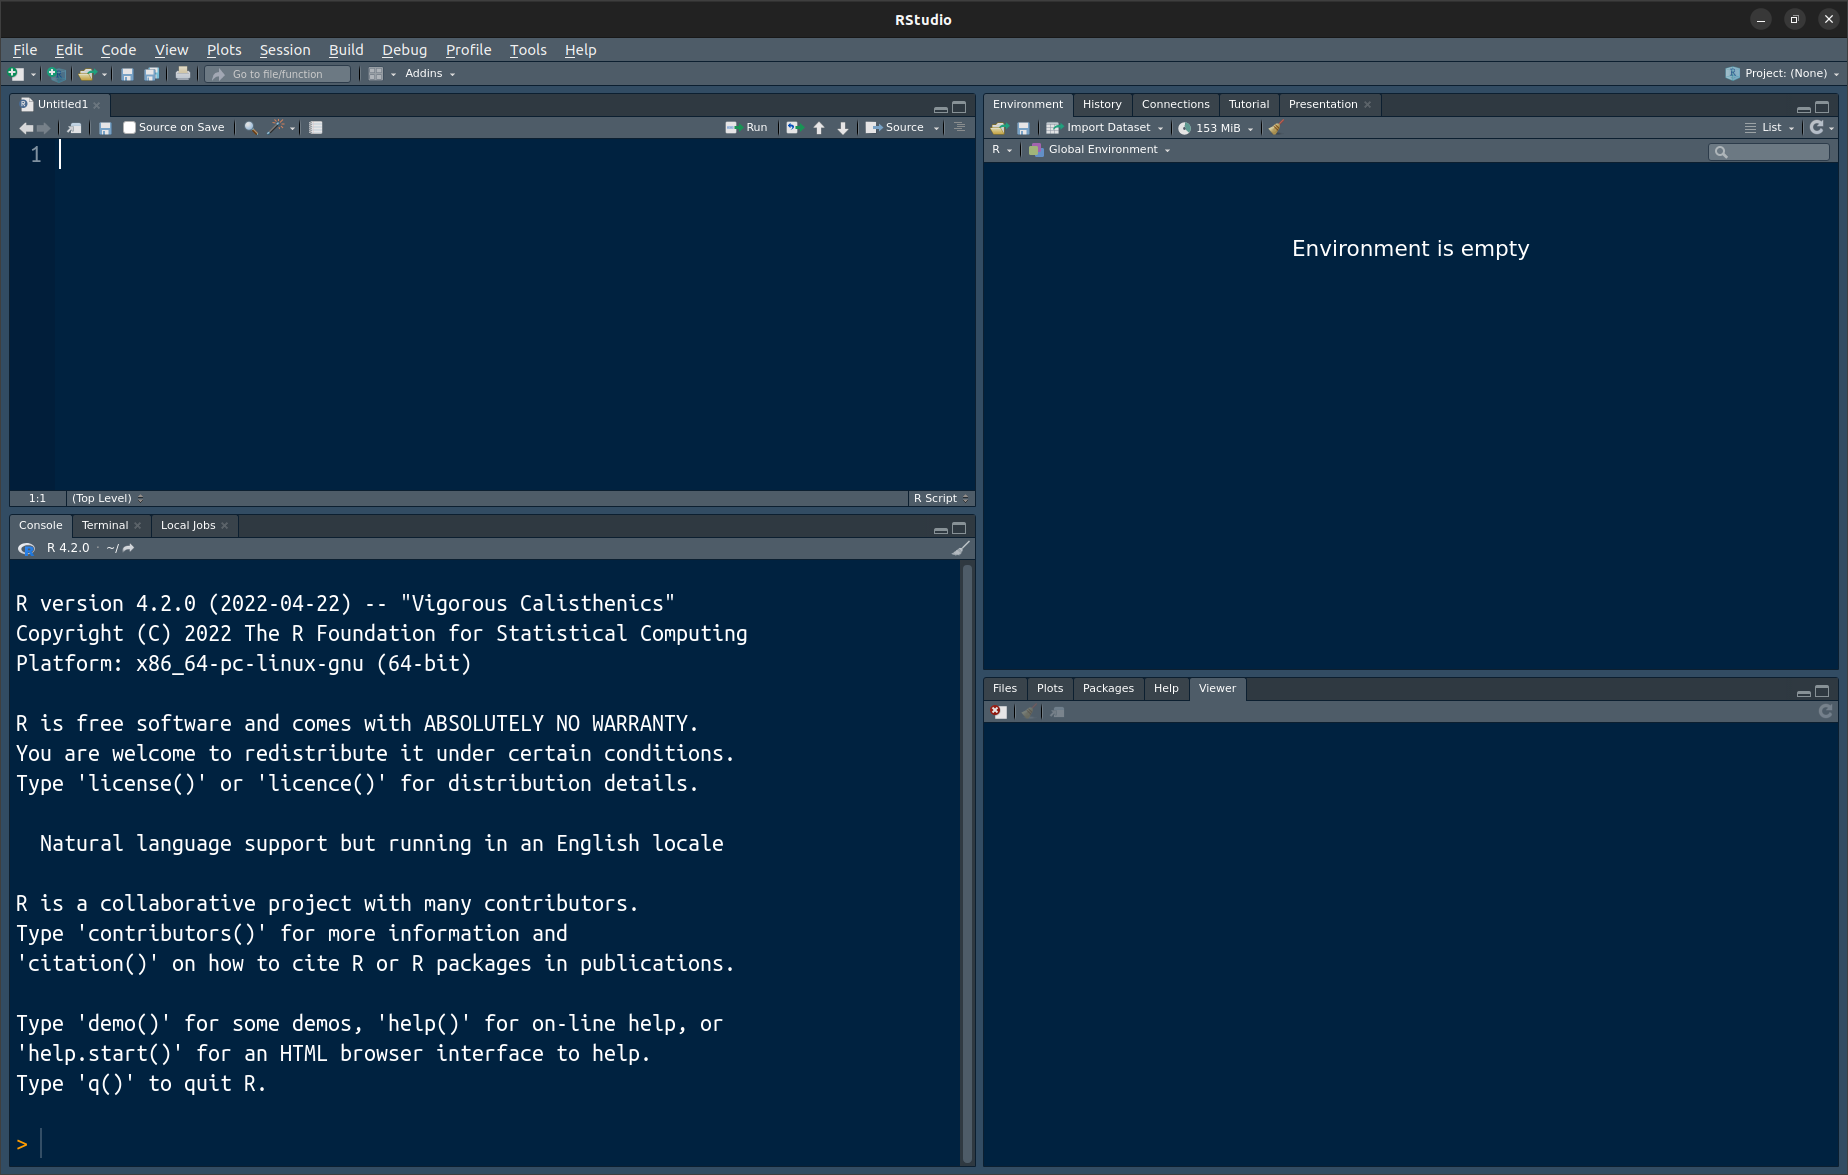
\includegraphics[max width = \textwidth]{figs/RStudio.png}
 \caption{RStudio mit links unten der R-Konsole, links oben einem Texteditor, rechts oben dem Verzeichnis über die Arbeitsumgebung (jetzt noch leer) und rechts unten allfällige Hilfeseiten und Grafiken.}
 \label{fig:rstudio}
\end{figure}

Bevor wir richtig loslegen, ist es sinnvoll, ein paar Einstellungen zu ändern.

\paragraph{Aufgabe 3.}
Klicken Sie dazu in RStudio auf \texttt{Tools > Global options\dots}
Stellen Sie sicher, dass unter \texttt{General > Basic} die Option
`Restore .RData into workspace at startup' \emph{nicht} angekreuzt ist
und dass bei `Save workspace to .RData on exit' die Option `never'
ausgewählt wurde.
Mit diesen Einstellungen vermeiden Sie, dass bei einem Neustart noch
alte Resultate und Objekte in der Arbeitsumgebung herumliegen,
die Ihre neuen Berechnungen beeinflussen, ohne dass Sie sich dessen
bewusst sind.
Weiter sollten Sie unter \texttt{Code > Editing} das Kästchen
`Use native pipe operator, |>' ankreuzen.
Was dieser `pipe operator' vermag, werden Sie schon bald merken.
Zum Schluss empfehle ich Ihnen, dass Sie unter \texttt{Code > Saving}
noch die `Default text encoding' auf UTF-8 wechseln. Das sollte
die Wahrscheinlichkeit erhöhen, dass Ihre Skripts auf anderen
Computern richtig angezeigt werden, wenn diese Sonderzeichen (wie Umlaute)
enthalten.

\section{R als Rechenmaschine}\label{sec:calculator}
Mit R verfügen Sie über eine Rechenmaschine.
Summen, Produkte und Quotienten können Sie
berechnen, indem Sie Befehle wie die unten stehenden
auf die Konsole (unten links) eintragen.
Das vorangestellte Symbol `>' gehört nicht zum Befehl selber,
aber Sie sehen es bereits auf der Konsole.
Auch die Ergebnisse gehören nicht zu
den Befehlen; diese werden auf der Konsole
angezeigt, sobald Sie den Befehl eingetragen
haben und mit \textsc{enter} bestätigt haben.

\begin{knitrout}
\definecolor{shadecolor}{rgb}{0.969, 0.969, 0.969}\color{fgcolor}\begin{kframe}
\begin{alltt}
\hlstd{> }\hlnum{10} \hlopt{+} \hlnum{7}
\end{alltt}
\begin{verbatim}
[1] 17
\end{verbatim}
\begin{alltt}
\hlstd{> }\hlnum{12} \hlopt{-} \hlnum{28}
\end{alltt}
\begin{verbatim}
[1] -16
\end{verbatim}
\begin{alltt}
\hlstd{> }\hlnum{7} \hlopt{*} \hlnum{3.5}
\end{alltt}
\begin{verbatim}
[1] 24.5
\end{verbatim}
\begin{alltt}
\hlstd{> }\hlnum{11} \hlopt{/} \hlnum{3}
\end{alltt}
\begin{verbatim}
[1] 3.6667
\end{verbatim}
\end{kframe}
\end{knitrout}

Für Exponentiation verwendet man den Operator `\textasciicircum':

\begin{knitrout}
\definecolor{shadecolor}{rgb}{0.969, 0.969, 0.969}\color{fgcolor}\begin{kframe}
\begin{alltt}
\hlstd{> }\hlnum{6} \hlopt{^} \hlnum{3}
\end{alltt}
\begin{verbatim}
[1] 216
\end{verbatim}
\end{kframe}
\end{knitrout}

Quadratwurzeln ziehen können Sie mit der \texttt{sqrt()}-Funktion.

\begin{knitrout}
\definecolor{shadecolor}{rgb}{0.969, 0.969, 0.969}\color{fgcolor}\begin{kframe}
\begin{alltt}
\hlstd{> }\hlkwd{sqrt}\hlstd{(}\hlnum{64}\hlstd{)}
\end{alltt}
\begin{verbatim}
[1] 8
\end{verbatim}
\end{kframe}
\end{knitrout}

Fürs Ziehen von beliebigen Wurzeln ist zu bemerken, dass $\sqrt[n]{x} = x^{1/n}$ gilt.
Somit lässt sich $\sqrt[3]{216}$ als $216^{1/3}$ berechnen:

\begin{knitrout}
\definecolor{shadecolor}{rgb}{0.969, 0.969, 0.969}\color{fgcolor}\begin{kframe}
\begin{alltt}
\hlstd{> }\hlnum{216} \hlopt{^} \hlstd{(}\hlnum{1}\hlopt{/}\hlnum{3}\hlstd{)}
\end{alltt}
\begin{verbatim}
[1] 6
\end{verbatim}
\end{kframe}
\end{knitrout}

Logarithmen berechnet man mit der \texttt{log()}-Funktion.
Die folgenden Befehlen berechnen so $\log_{10} 1000$ 
(d.h., wie oft muss man 10 mit sich selbst multiplizieren, um 1000 zu erhalten?) und 
$\log_2 256$ (d.h., wie oft muss man 2 mit sich selbst multiplizieren, um 256 zu erhalten?):

\begin{knitrout}
\definecolor{shadecolor}{rgb}{0.969, 0.969, 0.969}\color{fgcolor}\begin{kframe}
\begin{alltt}
\hlstd{> }\hlkwd{log}\hlstd{(}\hlnum{1000}\hlstd{,} \hlnum{10}\hlstd{)}
\end{alltt}
\begin{verbatim}
[1] 3
\end{verbatim}
\begin{alltt}
\hlstd{> }\hlkwd{log}\hlstd{(}\hlnum{256}\hlstd{,} \hlnum{2}\hlstd{)}
\end{alltt}
\begin{verbatim}
[1] 8
\end{verbatim}
\end{kframe}
\end{knitrout}

Für $\log_{10}$ und $\log_{2}$ existieren auch noch die Funktionen \texttt{log10()} bzw.\ \texttt{log2()}:
\begin{knitrout}
\definecolor{shadecolor}{rgb}{0.969, 0.969, 0.969}\color{fgcolor}\begin{kframe}
\begin{alltt}
\hlstd{> }\hlkwd{log10}\hlstd{(}\hlnum{1000}\hlstd{)}
\end{alltt}
\begin{verbatim}
[1] 3
\end{verbatim}
\begin{alltt}
\hlstd{> }\hlkwd{log2}\hlstd{(}\hlnum{256}\hlstd{)}
\end{alltt}
\begin{verbatim}
[1] 8
\end{verbatim}
\end{kframe}
\end{knitrout}

R respektiert die übliche Operatorrangfolge (z.B.\ Multiplikation vor Addition).
Verwenden Sie daher runde Klammern, um Berechnungen innerhalb eines Ausdrucks
vor anderen zu berechnen:

\begin{knitrout}
\definecolor{shadecolor}{rgb}{0.969, 0.969, 0.969}\color{fgcolor}\begin{kframe}
\begin{alltt}
\hlstd{> }\hlnum{8} \hlopt{*} \hlnum{0} \hlopt{+} \hlnum{4}
\end{alltt}
\begin{verbatim}
[1] 4
\end{verbatim}
\begin{alltt}
\hlstd{> }\hlnum{8} \hlopt{*} \hlstd{(}\hlnum{0} \hlopt{+} \hlnum{4}\hlstd{)}
\end{alltt}
\begin{verbatim}
[1] 32
\end{verbatim}
\end{kframe}
\end{knitrout}

Anderen Rechenoperationen widmen wir uns dann, wenn wir sie im Skript brauchen.

\section{Erweitungspakete installieren}
Es gibt für R jede Menge Erweiterungspakete,
mit denen man z.B.\ informative Grafiken
gestalten kann oder spezialisierte statistische
Modelle rechnen kann.
Mit dem unten stehenden Befehl installieren Sie das
\texttt{tidyverse}-Bündel: eine
Sammlung unterschiedlicher Pakete, die alle
auf der gleichen Philosophie basieren und 
die das Arbeiten mit Datensätzen wesentlich
erleichtern.

\paragraph{Aufgabe.}
Tippen Sie diesen Befehl in RStudio ins
Fenster links oben ein.
Und ich meine tatsächlich `tippen', nicht `selektieren, kopieren und einkleben': 
Sie werden viel mehr lernen, wenn Sie die Befehle in diesem Skript
abtippen als wenn Sie diese einfach aus dem PDF kopieren und einkleben!
Selektieren Sie dann die Zeile, klicken
Sie auf \texttt{Code, Run Selected Line(s)}
oder drücken Sie \textsc{ctrl + enter}
(Mac: \textsc{cmd + enter}).
Der Befehl wird nun an die Konsole (links unten)
weitergeleitet.
Im Prinzip können Sie diese kurzen Befehl auch
sofort in die Konsole eintragen, aber Sie sollten es sich angewöhnen,
im Texteditor zu arbeiten. Fehler können so wesentlich einfacher
aufgedeckt und behoben werden.
Ausserdem erleichtert das Arbeiten im Texteditor
das Dokumentieren Ihrer Analyse, da Sie Ihre Skripts abspeichern können.
\begin{knitrout}
\definecolor{shadecolor}{rgb}{0.969, 0.969, 0.969}\color{fgcolor}\begin{kframe}
\begin{alltt}
\hlstd{> }\hlkwd{install.packages}\hlstd{(}\hlstr{"tidyverse"}\hlstd{)}
\end{alltt}
\end{kframe}
\end{knitrout}

Für die Erweitungspakete, die im \texttt{tidyverse}-Bündel
zusammengepackt wurden, finden Sie unter \url{https://www.tidyverse.org/}
Anleitungen und weitere Informationen.

\section{R-Projekte}
Es ist sinnvoll, wenn die Skripts, Datensätze, Grafiken, usw.,
die Sie für ein Forschungsprojekt brauchen oder kreiert haben,
alle im gleichen Ordner (`Arbeitsordner') stehen.
Am besten richten Sie dazu für jedes Forschungsprojekt, an dem Sie beteiligt
sind (inklusive Seminar- und Masterarbeiten), ein R-Projekt ein.
Auch für diesen Kurs sollten Sie ein solches Projekt einrichten.

\paragraph{Aufgabe.}
Klicken Sie in RStudio auf \texttt{File, New Project..., New directory, Empty project} und geben Sie dem
Projekt einen Namen (z.B.\ Statistikkurs).
Für diesen Kurs brauchen Sie
die Optionen \texttt{Create a git repository}
und \texttt{Use renv with this project} nicht 
einzuschalten.\footnote{Erstere kann aber nützlich sein, wenn Sie 
mit anderen am gleichen R-Projekt arbeiten. Siehe dazu
\url{https://happygitwithr.com/}. Zum Nutzen
von \texttt{renv} erfahren Sie im nächsten Abschnitt mehr.}
Es wird jetzt ein Ordner kreiert, der eine Datei
mit der Endung \texttt{.Rproj} enthält.
Um das R-Projekt zu öffnen, können Sie diese Datei
öffnen oder das Projekt in RStudio unter
\texttt{File, Open Project...} auswählen.

Wenn Sie das Projekt geöffnet haben,
sollten Sie im Fenster rechts unten noch die Registerkarte
\texttt{Files} öffnen und mit \texttt{New Folder}
die Unterordner \texttt{data} und \texttt{figs} kreieren.
Die Datensätze, mit denen wir arbeiten werden, sollten Sie
in \texttt{data} ablegen; 
in \texttt{figs} werden wir Abbildungen (Grafiken) speichern.

\section{Softwareversionen und Updates}
R und seine Erweiterungspakete sind in ständiger Entwicklung.
Um ein Update der installierten R-Packages durchzuführen,
können Sie den Befehl \texttt{update.packages()} verwenden.
Um R selber auf den neusten Stand zu bringen, finde ich es
eigentlich am einfachsten, die alte Version komplett zu löschen
und die neue zu installieren. Danach muss ich dann aber die
Packages, die ich brauche, erneut installieren.
Dies kann recht mühsam sein, weshalb ich Ihnen empfehle,
solche Upgrades in der vorlesungsfreien Zeit durchzuführen
statt mitten im Semesterstress.

Aber Achtung: Es kommt nicht selten vor, dass alter R-Code
nach einem Update nicht mehr oder etwas anders funktioniert.
Für grössere Forschungsprojekte empfiehlt es sich daher,
die Option \texttt{Use renv with this project} anzukreuzen.
Diese sorgt dafür, dass die Versionen der Packages, die Sie 
im Projekt verwenden, als Teil des Projekts gespeichert werden.
Die verwendeten Packages müssen jedoch im Projekt neu installiert werden.
Auch wenn Sie nachher für ein anderes Projekt eine neuere
Version des Packages verwenden, werden die Befehle im ersten Projekt
noch mit der alten Version ausgeführt. Dies verringert die 
Gefahr, dass Ihr alter Code ein paar Jahre später nicht mehr funktioniert.
Für mehr Informationen, siehe \url{https://rstudio.github.io/renv/articles/renv.html}.

Für dieses Skript wurde R-Version 4.2.0 verwendet.
Eine Übersicht über die Packageversionen finden Sie im Anhang \ref{app:versions}.

\section{Software zitieren}
R und R-Pakete sind gratis und werden mehrheitlich
von anderen Forschenden entwickelt. Wenn Sie bei
Ihrer Arbeit sehr von R oder einem Erweiterungspaket
profitiert haben, ziehen Sie es dann bitte in Erwägung,
diesen Freiwilligen mit einer Referenz zu danken.

Eine Referenz für R erhalten Sie, wenn Sie 
den folgenden Befehl in die Konsole eintippen.
Den Output dieses Befehls wird hier im Skript nicht gezeigt.
\begin{knitrout}
\definecolor{shadecolor}{rgb}{0.969, 0.969, 0.969}\color{fgcolor}\begin{kframe}
\begin{alltt}
\hlstd{> }\hlkwd{citation}\hlstd{()}
\end{alltt}
\end{kframe}
\end{knitrout}

Wenn Sie ein bestimmtes Erweiterungspaket zitieren
möchten, stellen Sie den Namen des Pakets zwischen
Klammern und Anführungszeichen, etwa so:
\begin{knitrout}
\definecolor{shadecolor}{rgb}{0.969, 0.969, 0.969}\color{fgcolor}\begin{kframe}
\begin{alltt}
\hlstd{> }\hlcom{# Output nicht im Skript}
\hlstd{> }\hlkwd{citation}\hlstd{(}\hlstr{"tidyverse"}\hlstd{)}
\end{alltt}
\end{kframe}
\end{knitrout}

Es ist eine gute Idee, der Referenz an 
ein Erweitungspaket auch noch die Softwareversion 
hinzuzufügen. Es kann nämlich vorkommen, dass
gewisse Berechnungen je nach der Softwareversion
ein anderes---eventuell falsches---Ergebnis liefern.
Um die Softwareversion von R und eventuell geladenen
Erweitungspaketen abzurufen, können Sie den Befehl \texttt{sessionInfo()}
verwenden.
\begin{knitrout}
\definecolor{shadecolor}{rgb}{0.969, 0.969, 0.969}\color{fgcolor}\begin{kframe}
\begin{alltt}
\hlstd{> }\hlcom{# Output nicht im Skript}
\hlstd{> }\hlkwd{sessionInfo}\hlstd{()}
\end{alltt}
\end{kframe}
\end{knitrout}
% 
% Im obigen Output können Sie unter anderem sehen, dass
% ich Version 4.2.0 von R verwende und dass ich
% dieses Skript auf einer Ubuntu-Maschine geschrieben habe.
% Bei Ihnen wird dieser Output etwas anders aussehen---einerseits,
% weil Sie vielleicht eine andere R-Version auf einem anderen
% Betriebssystem verwenden, und andererseits, weil ich beim
% Schreiben dieses Skripts hinter den Kulissen Pakete verwende,
% die Sie gar nicht brauchen.
% 
% Um die Softwareversion eines spezifischen Erweitungspakets (vielleicht
% eines Pakets, das Sie noch nicht verwendet haben)
% abzurufen, können Sie den Namen dieses Pakets als Parameter der Funktion
% übergeben:
% 
% <<>>=
% sessionInfo("tidyverse")
% @
% 
% Unter \texttt{other attached packages} sehen Sie, dass bei mir
% Version 1.3.1 des \texttt{tidyverse}-Pakets installiert ist.
\section{Aufgaben}
\begin{enumerate}
  \item Ein nützliches Erweiterungspaket, das wir bald verwenden werden,
  ist das \texttt{here}-Package.
  \begin{enumerate}
    \item Installieren Sie das \texttt{here}-Package.
    \item Wer hat das \texttt{here}-Package geschrieben?
    \item Welche Version des \texttt{here}-Pakets haben Sie installiert?
  \end{enumerate}
  
  \item Das Arbeiten im Texteditor erleichtert das Dokumentieren
  von Analysen.
  \begin{enumerate}
    \item Kreieren Sie ein neues R-Skript (\texttt{File, New File, R Script})
  und tragen Sie hier die R-Befehle aus Abschnitt \ref{sec:calculator} ein.
  
    \item Fügen Sie am Ende des Skripts noch eine Zeile mit dem folgenden Befehl hinzu:
\begin{knitrout}
\definecolor{shadecolor}{rgb}{0.969, 0.969, 0.969}\color{fgcolor}\begin{kframe}
\begin{alltt}
\hlstd{> }\hlkwd{sessionInfo}\hlstd{()}
\end{alltt}
\end{kframe}
\end{knitrout}

    \item Speichern Sie das Skript mit der Endung \texttt{.R}
  (z.B.\ \texttt{rechenmaschine.R}).
  
    \item Klicken Sie dann auf \texttt{File, Compile Report\dots} und wählen
  Sie dort HTML als Outputformat aus. (Eventuell müssen Sie
  dann noch ein zusätzliches Paket installieren.)
  Hiermit wird eine HTML-Datei hergestellt, die sowohl
  die Befehle als auch deren Output enthält.
  Dank des Outputs von \texttt{sessionInfo()} ist auch klar,
  welche Softwareversionen Sie für Ihre Berechnungen verwendet haben.
  
  Wenn der R-Code Syntaxfehler enthält, kann übrigens keine
  HTML-Datei hergestellt werden. So bietet das Arbeiten 
  mit Skripts und HTML-Berichten eine minimale Qualitätskontrolle.
  
    \item Fügen Sie am Anfang Ihres R-Skripts noch folgende Zeilen hinzu.
\begin{verbatim}
#' ---
#' author: '<Ihr Name>'
#' title: 'R als Rechenmaschine'
#' ---
\end{verbatim}
    Kompilieren Sie den HTML-Bericht erneut.

    \item Übrigens können Sie dem Bericht auch noch Text hinzufügen
    und seine Struktur mit Überschriften klarer machen. Stellen Sie
    hierzu den Textzeilen die Symbolen \texttt{\#'} voran. Fügen
    Sie zum Beispiel dieses Textchen noch irgendwo hinzu und 
    kompilieren Sie den Bericht erneut:
\begin{verbatim}
#' Um Ihre Überlegungen und Erkenntnisse zu dokumentieren,
#' können Sie Absätze wie diese in Ihre Skripts einbauen.
#' Solche Absätze werden von R <i>ignoriert</i>, aber sind
#' sowohl im Skript als auch im HTML-Bericht <b>sichtbar</b>.
#' Sie können hier auch HTML-Markup verwenden.

#' <h1>Beschriftung (1. Stufe)</h1>
#' Lorem ipsum.
 
#' <h2>Beschriftung (2. Stufe)</h2>
#' <h3>Beschriftung (3. Stufe, etc.)</h3>
\end{verbatim}

    \end{enumerate}
\end{enumerate}


\chapter{Arbeiten mit Datensätzen}\label{ch:datenaufbereiten}
Die erste Hürde, die es bei einer quantitativen Analyse
zu überwinden gilt, ist, die Daten so zu organisieren,
dass diese überhaupt analysierbar sind. Hat man dies
geschafft, muss man die Daten noch in das Computerprogramm, 
mit dem man sie analysieren wird (hier: R), einlesen.
Öfters muss man die eingelesen Datensätze anschliessend
mit anderen Datensätzen kombinieren und umgestalten
und in der Regel will man auch noch gewisse Informationen
aus den Datensätzen herauslesen. Dieses Kapitel ist
diesen Schritten gewidmet.

\section{Daten organisieren}
Stellen Sie sich die folgende Datenerhebung vor.
Sie möchten untersuchen, wie sich die Fähigkeit,
die Bedeutung von Wörtern in einer nicht beherrschten 
Sprache auf der Basis ihrer Ähnlichkeit zu Wörtern
in beherrschten Sprachen zu erschliessen, im Laufe
des Lebens verändert. Dazu legen Sie einer Reihe von
deutschsprachigen Versuchspersonen unterschiedlichen
Alters eine Anzahl geschriebener schwedischer Wörter vor
und bitten Sie sie, diese ins Deutsche zu übersetzen.
Der Übersichtlichkeit halber werden hier die Übersetzungen
von vier Versuchspersonen für fünf Wörter gezeigt,
und zwar für jede Versuchsperson in der Reihenfolge,
in der die Wörter übersetzt wurden.

\begin{itemize}
\item Versuchsperson 1034. Frau, 51 Jahre.
\begin{itemize}
\item Wort: \textit{söka}. Übersetzung: \textit{Socken} (falsch).
\item Wort: \textit{försiktig}. Übersetzung: \textit{vorsichtig} (richtig).
\item Wort: \textit{mjölk}. Übersetzung: \textit{Milch} (richtig).
\item Wort: \textit{behärska}. Keine Übersetzung gegeben.
\item Wort: \textit{fiende}. Übersetzung: \textit{finden} (falsch).
\end{itemize}

\item Versuchsperson 2384. Frau, 27 Jahre.
\begin{itemize}
\item Wort: \textit{fiende}. Keine Übersetzung gegeben.
\item Wort: \textit{behärska}. Keine Übersetzung gegeben.
\item Wort: \textit{försiktig}. Übersetzung: \textit{vorsichtig} (richtig).
\item Wort: \textit{mjölk}. Übersetzung: \textit{Milch} (richtig).
\item Wort: \textit{söka}. Übersetzung: \textit{Socke} (falsch).
\end{itemize}

\item Versuchsperson 8667. Frau, 27 Jahre.
\begin{itemize}
\item Wort: \textit{mjölk}. Übersetzung: \textit{Milch} (richtig).
\item Wort: \textit{behärska}. Keine Übersetzung gegeben.
\item Wort: \textit{fiende}. Übersetzung: \textit{finden} (falsch).
\item Wort: \textit{söka}. Übersetzung: \textit{suchen} (richtig).
\item Wort: \textit{försiktig}. Übersetzung: \textit{vorsichtig} (richtig).
\end{itemize}

\item Versuchsperson 5901. Mann, 15 Jahre.
\begin{itemize}
\item Wort: \textit{behärska}. Übersetzung: \textit{beherrschen} (richtig).
\item Wort: \textit{mjölk}. Übersetzung: \textit{milch} (sic.) (richtig).
\item Wort: \textit{försiktig}. Übersetzung: \textit{vorsichtig} (richtig).
\item Wort: \textit{fiende}. Übersetzung: \textit{feinde} (sic.) (richtig; eigentlich \textit{Feind}).
\item Wort: \textit{söka}. Übersetzung: \textit{socken} (sic.) (falsch).
\end{itemize}
\end{itemize}

Wie trägt man solche Angaben am besten in ein Spreadsheet ein?
Bevor wir uns ein paar Faustregeln anschauen, möchte ich ein bisschen
Werbung für ein Spreadsheetprogramm machen, dass Sie vielleicht noch
nicht kennen.

\paragraph{Ein kostenloses Spread\-sheetprogramm.}
\href{http://libreoffice.org}{LibreOffice.org} ist eine
kostenlose Applikationssuite, die---wie Microsoft Office---aus 
einem Textbearbeitungsprogramm (Write), einem Spread\-sheetprogramm
(Calc), einem Präsentationsprogramm (Impress) usw., besteht.
Selber finde ich LibreOffice Calc nützlicher als MS Excel,
weil man beim Speichern von Spread\-sheets gewisse Einstellungen
viel einfacher ändern kann. Darauf werden wir später zurückkommen.

\subsection{Lange Datensätze sind praktischer als breite}
Wir befassen uns in diesem Kurs mit sog.\ rechteckigen Datensätzen,
d.h., Datensätze, in denen die Informationen in Zeilen und Spalten
organisiert werden und in denen alle Zeilen und Spalten gleich lang sind.
(Beispiele von anderen Datensatzformaten sind XML und JSON.)
Die zwei üblichsten Formate, in denen Datensätze organisiert werden,
sind das breite und das lange Format.
Im breiten Format werden alle Angaben zu einer bestimmten
\textbf{Erhebungseinheit} (z.B., zu einer Versuchsperson) in die gleiche
Zeile eingetragen. In unserem Beispiel könnte ein breiter Datensatz
wie in Abbildung \ref{fig:wide_data_subject} aussehen (7 Spalten werden nicht gezeigt).
Bemerken Sie, dass es für jedes Wort drei Spalten gibt:
eine, in der steht, an welcher Stelle das Wort übersetzt wurde;
eine, in der die Übersetzung steht;
und eine, in der vermerkt wird, ob die Übersetzung richtig war.
Auch die Anordnung in Abbildung \ref{fig:wide_data_item}, in der es eine Zeile pro Wort gibt
und alle Übersetzungen für dieses Wort auf der gleichen Zeile
stehen, ist ein Beispiel eines breiten Datensatzes (10 Spalten nicht
werden nicht gezeigt).

\begin{figure}[tp]
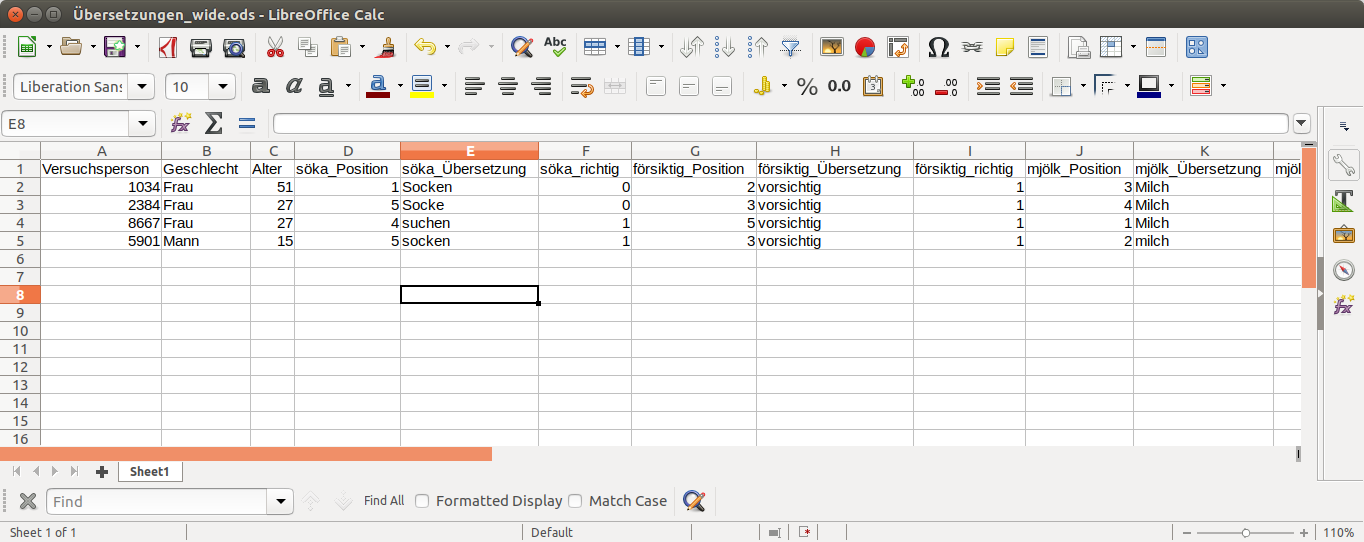
\includegraphics[width = \textwidth]{figs/wide_data_subject.png}
\caption{Ein breiter Datensatz mit einer Zeile pro Versuchsperson.}
\label{fig:wide_data_subject}
\end{figure}

\begin{figure}[tp]
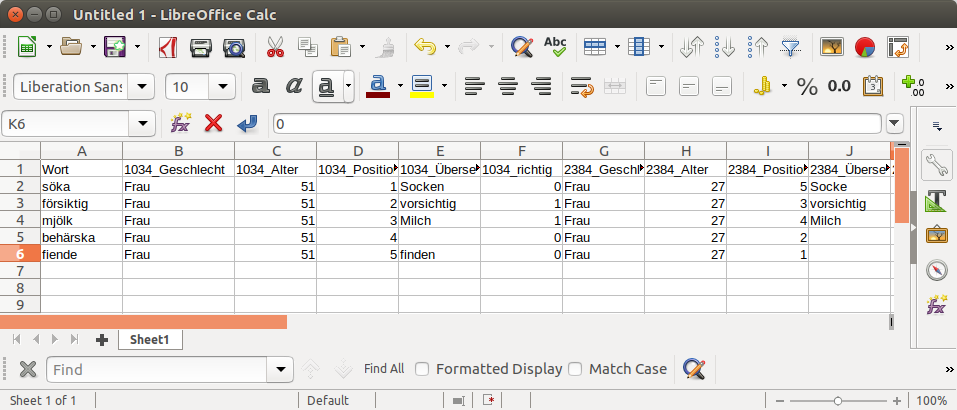
\includegraphics[width = \textwidth]{figs/wide_data_item.png}
\caption{Ein breiter Datensatz mit einer Zeile pro Stimulus.}
\label{fig:wide_data_item}
\end{figure}

Im langen Format werden die Angaben zu einer \textbf{Beobachtungseinheit}
in der gleichen Zeile arrangiert. Eine Definition von `Erhebungseinheit'
und `Beobachtungseinheit' ist schwierig zu geben \citep[siehe][]{Wickham2014}
und würde ausserdem wenig bringen. In diesem Beispiel wären die 
Beobachtungseinheiten aber die einzelnen Übersetzungen. Die gleichen
Daten im langen Format könnten aussehen wie in Abbildung \ref{fig:long_data}.
Es ist in der Regel wesentlich einfacher mit langen Datensätzen als mit
breiten zu arbeiten. Und falls es trotzdem einmal nötig sein sollte, mit
einem breiten Datensatz zu arbeiten: Lange Datensätze zu breiten zu 
konvertieren, ist einfacher als umgekehrt; siehe hierzu Abschnitt \ref{sec:pivot}.

\begin{figure}[tp]
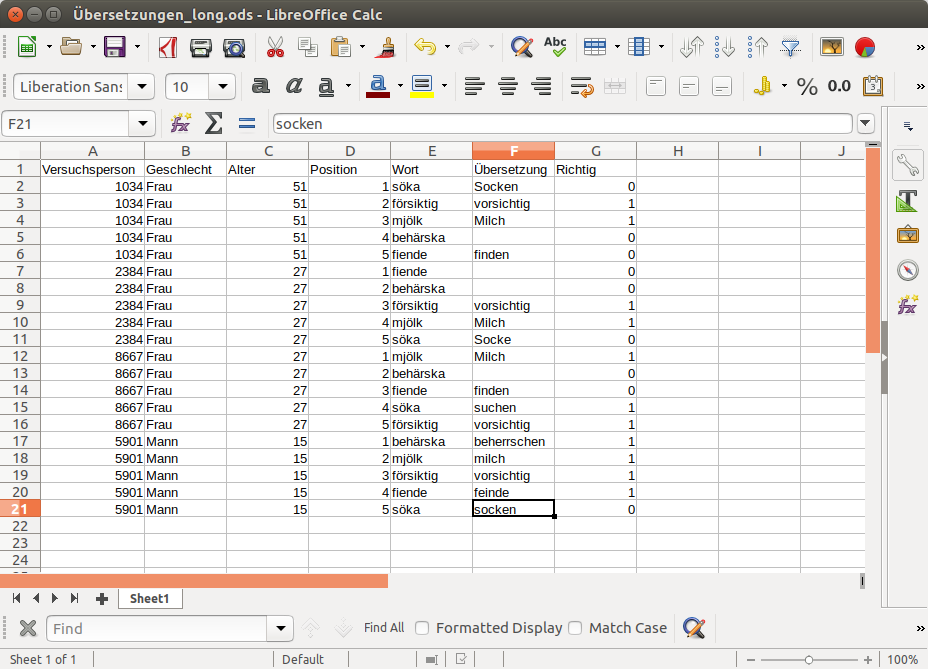
\includegraphics[width = \textwidth]{figs/long_data.png}
\caption{Ein langer Datensatz mit einer Zeile pro Stimulus pro Versuchsperson. Lange Datensätze sind in der Regel einfacher zu verwalten und zu analysieren als breite.}
\label{fig:long_data}
\end{figure}

Um zu vermeiden, dass das absichtliche oder versehentliche Löschen
einer Zeile dazu führt, dass die anderen Zeilen nicht mehr
interpretiert werden können, werden die Angaben zu den Versuchspersonen
in jeder Zeile wiederholt. Lassen Sie weder im langen noch im
breiten Format Informationen weg, die man einer anderen
Zeile entnehmen kann. Also \emph{nicht} so wie in Abbildung \ref{fig:leere_zellen}!

\begin{figure}[tp]
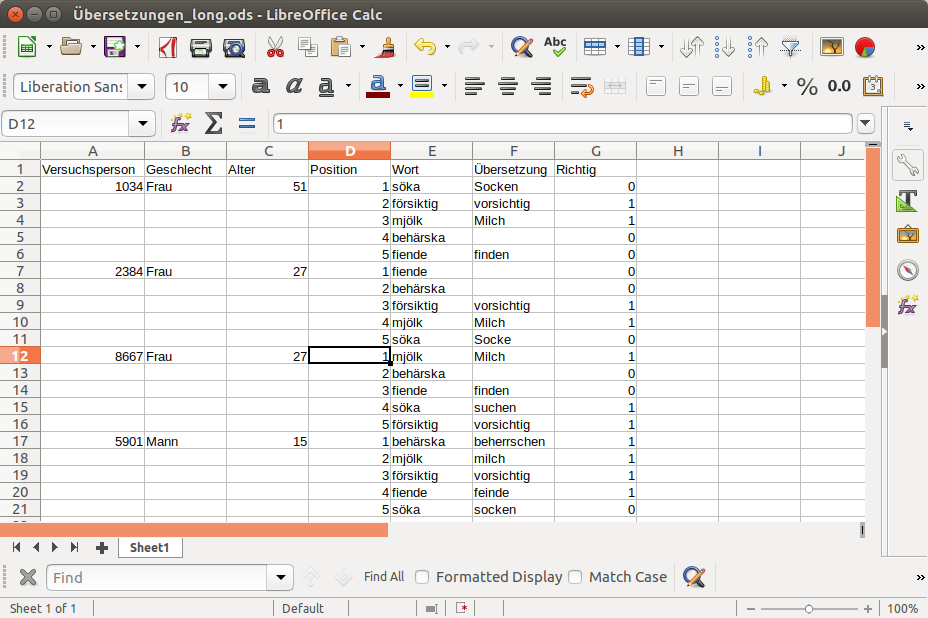
\includegraphics[width = \textwidth]{figs/long_data_nicht_so.png}
\caption{Nicht so! In diesem Datensatz wurden mehrere Zellen leer gelassen, da man deren
Inhalt anderen Zellen entnehmen kann. Dies wird bei einer Analyse aber zu Schwierigkeiten führen. Ausserdem kann das Löschen einer Zeile dafür sorgen,
dass die Infos auf anderen Zeilen nicht mehr rekonstruiert werden können.}
\label{fig:leere_zellen}
\end{figure}

Bemerken Sie auch, dass es eine Spalte gibt, welche die Reihenfolge,
in der die Wörter übersetzt wurden, explizit macht. Im Prinzip könnte
man diese Information aus der Struktur des Datensatzes ableiten.
Indem man diese Information jedoch explizit hinzufügt, vermeidet man,
dass sie verloren geht, wenn der Datensatz anders sortiert wird.

Sowohl breite als auch lange Datensätze sind \textbf{rechteckig}:
\begin{itemize}
\item Sie haben eine Anzahl Zeilen und Spalten. Alle Zeilen sind gleich lang. Dies gilt auch für die Spalten.
\item Es gibt keine komplett leeren Zeilen und Spalten. Einzelne leere Zellen
gibt es öfters schon, aber es ist nicht so, dass es Angaben in Spalten A--D
gibt, überhaupt keine in Spalten E--F und dann wieder welche in Spalte G.
\item In der Regel haben alle Spalten einen Namen. Manchmal kommt es zwar vor,
dass keine einzige Spalte einen Namen hat, aber geben Sie nicht ein paar Spalten
einen Namen und anderen nicht.
\item Alle Spaltennamen stehen in \emph{einer} Zeile. Die Spaltenbezeichnungen stellen
sich also nicht aus mehreren Zellen zusammen.
\end{itemize}

Zum Vergleich: Das Spread\-sheet in Abbildung \ref{fig:berechnungen_im_Spreadsheet} zeigt einen
nicht-rechteckigen Datensatz. Die Zusammenfassungen unten
haben in diesem Datensatz nichts zu suchen und würden
beim Einlesen zu Problemen führen.

\begin{figure}[tp]
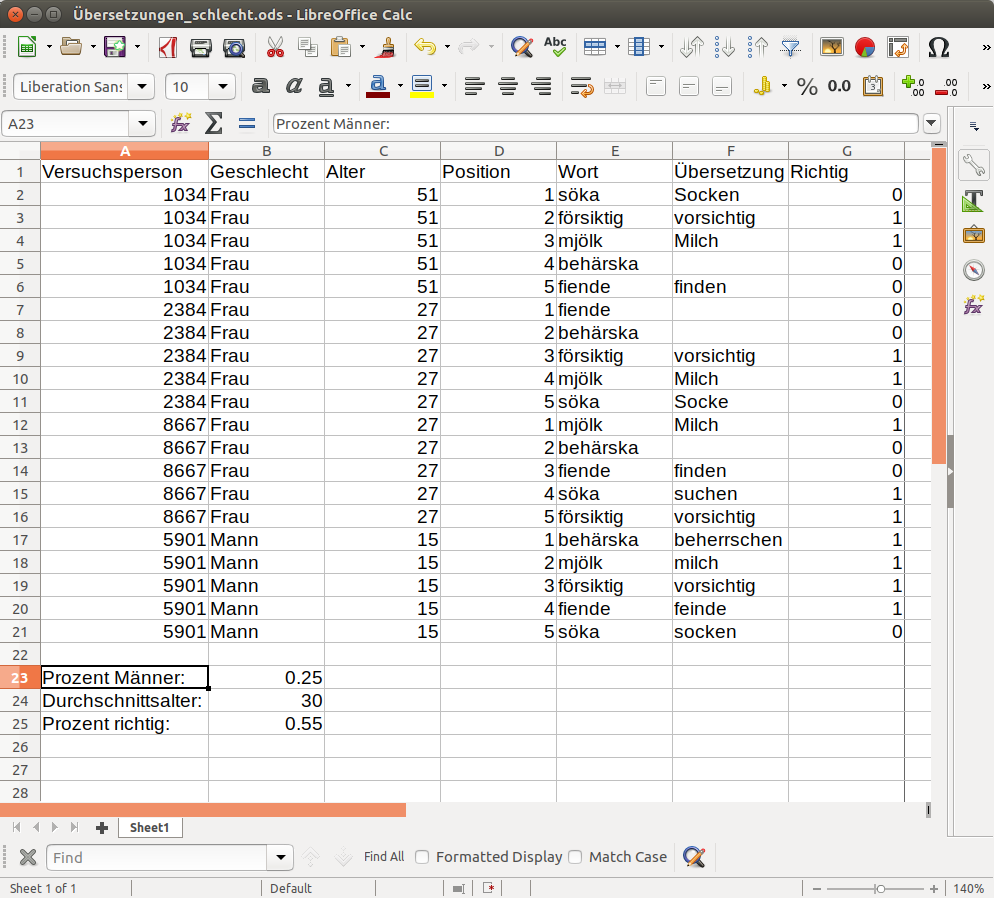
\includegraphics[width = \textwidth]{figs/datensatz_schlecht.png}
\caption{Nicht so! Dieser Datensatz ist nicht rechteckig: ``Prozent Männer:'' ist keine Versuchspersonnummer, und ``0.25'' ist kein Geschlecht. Ausserdem ist Zeile 22 komplett leer.}
\label{fig:berechnungen_im_Spreadsheet}
\end{figure}

\subsection{Kurze, aber selbsterklärende Bezeichnungen verwenden}
Machen Sie sich die spätere Analyse einfacher, indem Sie den
Spalten und anderen Angaben in Ihren Datensätzen deutliche Namen geben.
Dadurch vermeiden Sie, dass Sie während der Analyse
ständig wieder nachschlagen müssen, was die
Angaben überhaupt heissen. Dies verringert wiederum
die Wahrscheinlichkeit, dass Sie Fehler machen.

Ein paar Beispiele:

\begin{itemize}
\item Sie werten einen Fragebogen aus. Machen
Sie in jeder Spalte deutlich, worum es in den Fragen 
ging. Vermeiden Sie also Spaltennamen wie `Q3' oder 
`Frage8'. Verwenden Sie stattdessen Spaltennamen
wie `DiplomVater' (wenn die Frage war, welchen
Schulabschluss der Vater der Gewährsperson hat)
oder `DialectUse' (wenn die Frage war, wie oft
die Gewährsperson Dialekt redet).

\item Wenn Sie eine Spalte namens `Geschlecht' haben,
die mit Nullen und Einsen gefüllt ist, müssten Sie
ständig nachschlagen, ob 0 jetzt für `Frau' oder 
`Mann' steht. Verwenden Sie stattdessen lieber direkt
`Frau' und `Mann', oder sogar `f' und `m'.
Eine andere Möglichkeit ist, dass Sie die Spalte
zu `Frau' umbenennen, sodass es deutlich
ist, dass eine 1 heisst, dass die Gewährsperson
eine Frau war, und eine 0, dass es sich um einen
Mann handelte.

\item Verwenden Sie eher kurze Bezeichnungen.
In der späteren Analyse werden Sie nämlich
insbesondere 
die Spaltennamen mehrmals wieder eintippen müssen.
Vermeiden Sie daher Spaltennamen wie `wie\_oft\_sprechen\_Sie\_Hochdeutsch' und verwenden Sie stattdessen
`use\_hochdeutsch' oder Ähnliches.
\end{itemize}

Am besten verwenden Sie übrigens keine Leertasten
und Lesezeichen in den Spaltennamen.


\subsection{Fehlende Angaben unzweideutig vermerken}
Im Beispiel oben habe ich fehlende Übersetzungen
einfach leer gelassen. Daraus kann ich ableiten,
dass der Versuchsperson das Wort zwar vorgelegt
wurde, aber sie dieses nicht übersetzt hat.
Es wäre jedoch auch möglich gewesen, dass
einigen Versuchspersonen bestimmte Wörter
gar nie vorgelegt wurden, z.B.\
aufgrund eines Softwarefehlers.
Es wäre wichtig, solche Fälle 
von den ersten zu unterscheiden,
indem man diese Fälle mit einer Kürzel (z.B.
`NA' für `not available' oder `not applicable')
vermerkt.

Gegebenenfalls kann man auch mehrere Kürzel
verwenden, um unterschiedliche Gründe für
das Nicht-Vorhanden-Seins voneinander zu unterscheiden.
In der Regel ist es aber am einfachsten, sämtliche
fehlende Daten mit `NA' zu vermerken und
den Grund hierfür in eine Kommentarspalte einzutragen.

Verwenden Sie aber keine Zahlen
(wie -99 oder -9999), um fehlende Angaben zu vermerken.
Der Grund ist, dass solche Zahlen manchmal zulässige
Werte sind. Ausserdem können solche Angaben
schwieriger auf den ersten Blick erkannt werden,
wenn man eine Zusammenfassung des Datensatzes generiert.

\subsection{Mehrere kleinere Datensätze sind handlicher als ein riesiger}
\label{sec:mehrere_kleine}
In den Spread\-sheets oben wurden bestimmte
Informationen mehrfach wiederholt. Zum Beispiel
musste man bei den Übersetzungen von Versuchsperson
1034 fünf Mal eintragen, dass sie eine Frau im Alter
von 51 Jahren war. In diesem Fall ist der Datensatz
trotz wiederholten Informationen übersichtlich.
Wenn man sich aber überlegt, dass in der Regel für
jede Versuchsperson viel mehr Informationen
vorliegen (z.B., Daten aus einem Hintergrundsfragebogen)
und dass man öfters auch Informationen zu den verwendeten
Stimuli (hier: den Wörtern) mit einbeziehen will,
wird klar, dass man es schnell mit grossen Datensätzen
zu tun hat, in denen viele Informationen mehrfach
wiederholt werden.

Um die Übersicht zu bewahren und um sich eine 
Menge Tipp- oder Kopierarbeit zu sparen, lohnt
es sich, statt eines grossen Datensatzes
mehrere kleinere zu verwalten. In unserem Beispiel
würde man dann ein Spread\-sheet mit Informationen
zu den Versuchspersonen gestalten (Abbildung \ref{fig:versuchspersonen}).
Daneben kann man noch ein Spread\-sheet mit Informationen
zu den Wörtern anfertigen (Abbildung \ref{fig:woerter}).
In einem dritten Spread\-sheet kann man dann die Antworten bei der 
Übersetzungsaufgabe aufführen (Abbildung \ref{fig:uebersetzungen}).

\begin{figure}[tp]
\centering
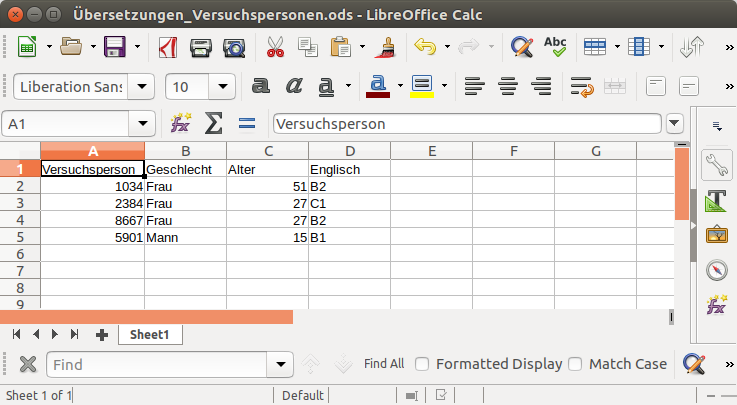
\includegraphics[max width = 0.7\textwidth]{figs/versuchspersonen.png}
\caption{Ein erster Datensatz mit Informationen, die nur die Versuchspersonen betreffen.}
\label{fig:versuchspersonen}
\end{figure}


\begin{figure}[tp]
\centering
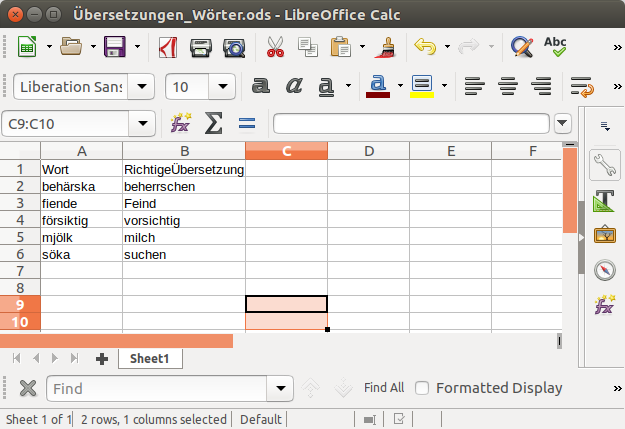
\includegraphics[max width = 0.7\textwidth]{figs/woerter.png}
\caption{Ein zweiter Datensatz mit Informationen, die nur die Stimuli betreffen.}
\label{fig:woerter}
\end{figure}

\begin{figure}[tp]
\centering
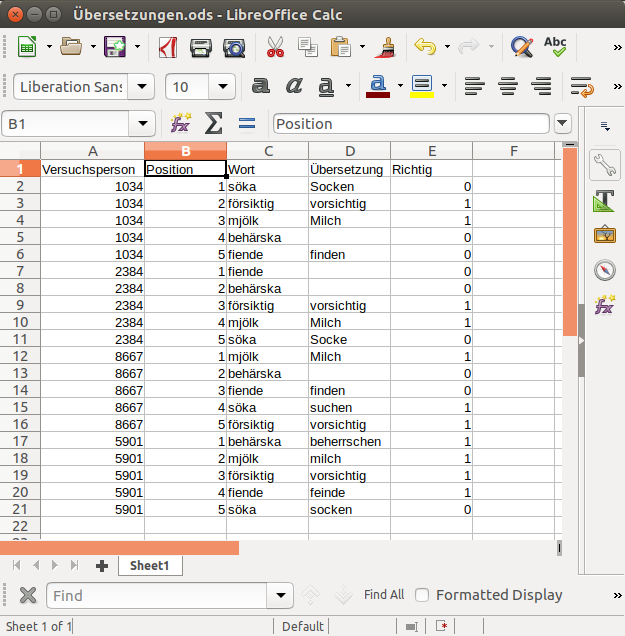
\includegraphics[max width = 0.7\textwidth]{figs/uebersetzungen.png}
\caption{Ein dritter Datensatz, in dem die Übersetzungen aufgeführt werden.}
\label{fig:uebersetzungen}
\end{figure}

Da im letzten Spread\-sheet sowohl eine Spalte mit
den Identifikationen der Versuchspersonen als
auch mit den Bezeichnungen der Stimuli vorhanden ist,
können ihm die Informationen aus den ersten zwei kleineren
Datensätzen nachher problemlos hinzugefügt werden.
Wie man dies in R machen kann, erfahren Sie in Abschnitt \ref{sec:join}.

\subsection{Weitere Bemerkungen}
\begin{itemize}

\item Beachten Sie Gross- und Kleinschreibung. Für manche Statistikprogramme ist `Frau` gleich `frau', für andere (darunter R) nicht.

\item Sonderzeichen, wie Umlaute, führen manchmal zu Problemen.

\item Beachten Sie Leerzeichen. Für ein Computer ist `Mann' nicht gleich `Mann ' (mit Leerzeichen).

\item Wenn Sie in Ihren Spread\-sheets gerne mit Farben arbeiten: Diese gehen verloren, wenn Sie das Spread\-sheet in R einlesen. Wenn die Farben Informationen kodieren, die nicht den Angaben
im Spread\-sheet entnommen werden können, fügen Sie diese Informationen also besser noch selbst hinzu.

\item Arbeiten Sie möglichst wenig im Spreadsheet!
Nachdem Sie die Daten eingetragen haben, sollten Sie grundsätzlich nicht mehr
im Spreadsheet, sondern in R selber arbeiten. Also nicht in Excel herumrechnen,
sortieren, kopieren, kleben, neu formattieren usw. Wenn Sie diese Schritte in
R ausführen und Ihren Code speichern, ist eindeutig festgelegt, wie Sie den Datensatz
umgestaltet haben, um Grafiken zu zeichnen und Modelle zu rechnen.
Der ursprüngliche Datensatz bleibt dabei aber unverändert, sodass Sie immer
wieder aufs Original zurückgreifen können.
\end{itemize}


\section{Datensätze einlesen}
Wenn die Daten in einem analysierbaren Format vorliegen,
besteht die nächste Herausforderung darin, diese in R
einzulesen. Wir behandeln hier nur zwei Fälle:
das Einlesen von Excel-Spreadsheets im XLS(X)-Format
und das Einlesen von Spreadsheets im CSV-Format.

\subsection{Excel-Spreadsheets (XLS, XLSX)}
Speichern Sie den Datensatz \texttt{uebersetzungen.xlsx}
im Ordner \texttt{data} in Ihrem Arbeitsordner.
Dieser Datensatz ist eine Exceldatei, die aus einem einzigen
Spread\-sheet besteht. Um ihn in R einzulesen,
verwenden wir die Funktion \texttt{read\_excel()}
aus dem \texttt{readxl}-Package. Dieses Package ist Teil
des \texttt{tidyverse}-Bündels, das wir bereits installiert haben.
Wenn wir seine Funktionen aber verwenden möchten, müssen wir
das Package noch laden. Das machen wir mit der Funktion \texttt{library()}:
\begin{knitrout}
\definecolor{shadecolor}{rgb}{0.969, 0.969, 0.969}\color{fgcolor}\begin{kframe}
\begin{alltt}
\hlstd{> }\hlkwd{library}\hlstd{(readxl)}
\end{alltt}
\end{kframe}
\end{knitrout}

Wenn keine Fehlermeldung kommt, ist gut!

\paragraph{Aufgabe.} Welche Version von \texttt{readxl}
haben Sie installiert?

Installieren müssen Sie Packages übrigens nicht immer wieder,
aber Sie müssen die Packages, deren Funktionen Sie 
verwenden schon bei jeder neuen Session wieder
mit \texttt{library()} laden.

Um den Datensatz einzulesen, verwenden wir nun die Funktion
\texttt{read\_excel()}, der wir den Pfad zur Exceldatei übergeben.
R akzeptiert sowohl absolute als auch relative Pfade,
aber damit Sie bereits jetzt gute Gewohnheiten entwickeln,
verweisen wir auf Dateien ab dem Ordner, in der sich die .Rproj-Datei
des aktuellen Projekts befindet. Das geht am einfachsten mit der \texttt{here()}-Funktion aus dem \texttt{here}-Package, das wir auch noch laden müssen.
Für unsere jetzigen Zwecke ist die Verwendung von \texttt{here()}
eigentlich übertrieben, aber für grössere Projekte ist es eine
sehr nützliche Funktion, sodass wir sie hier sofort verwenden.
\begin{knitrout}
\definecolor{shadecolor}{rgb}{0.969, 0.969, 0.969}\color{fgcolor}\begin{kframe}
\begin{alltt}
\hlstd{> }\hlkwd{library}\hlstd{(here)}
\end{alltt}


{\ttfamily\noindent\itshape\color{messagecolor}{here() starts at /home/jan/ownCloud/statintro}}\begin{alltt}
\hlstd{> }\hlstd{translations} \hlkwb{<-} \hlkwd{read_excel}\hlstd{(}\hlkwd{here}\hlstd{(}\hlstr{"data"}\hlstd{,} \hlstr{"uebersetzungen.xlsx"}\hlstd{))}
\end{alltt}
\end{kframe}
\end{knitrout}

Wie Sie sehen, erkennt die \texttt{here()}-Funktion, dass sich (bei mir)
die .Rproj-Datei im Ordner \texttt{home/jan/ownCloud/StatIntro2022}
befindet. Bei Ihnen wird dieser Pfad natürlich anders aussehen. 
Die Alternative ohne \texttt{here()} und mit einem relativen Pfad sähe übrigens so aus:
\begin{knitrout}
\definecolor{shadecolor}{rgb}{0.969, 0.969, 0.969}\color{fgcolor}\begin{kframe}
\begin{alltt}
\hlstd{> }\hlstd{translations} \hlkwb{<-} \hlkwd{read_excel}\hlstd{(}\hlstr{"data/uebersetzungen.xlsx"}\hlstd{)}
\end{alltt}
\end{kframe}
\end{knitrout}
Der Vorteil von der \texttt{here()}-Funktion ist,
dass der Befehl auch genau so funktioniert, wenn das
Skript, in dem es vorkommt, in einem Unterordner gespeichert ist:
Die einzulesende Datei wird ab dem \textit{project root} gesucht,
nicht ab dem Pfad des Skripts.

Angezeigt wird der Datensatz übrigens noch nicht, aber im Fenster rechts oben
sollten Sie jetzt ein Objekt namens \texttt{translations} sehen,
zusammen mit der Angabe `20 obs.\ of 5 variables'.

Der Datensatz ist nun zugänglich in einem sog.\ \textit{tibble} namens \texttt{translations}.\footnote{Rechteckige Datensätze heissen in R eigentlich \textit{data frames}. \textit{Tibbles} sind die Entsprechung von \textit{data frames} in den \textit{tidyverse}-Paketen, darunter auch das Paket \texttt{readxl}. Wer schon viel Erfahrung mit R hat, wird im Laufe des Skripts vielleicht ein paar subtile Unterschiede zwischen \textit{data frames} und \textit{tibbles} feststellen, aber im Grossen und Ganzen sind sie klein.\label{fn:tibble}}

\medskip

\begin{framed}
\noindent \textbf{Einschub: <-, = und ==.}
Die Symbolenfolge \texttt{<-} ist der \textit{assignment operator}.
Sie kreiert ein neues Objekt im Arbeitsgedächtnis bzw. überschreibt ein bereits
vorhandenes Objekt. Dieses Objekt trägt den Namen links von \texttt{<-}.
Kürzel in RStudio: \textsc{alt} + \textsc{-}.

Oft wird auch das Ist-Gleich-Zeichen (\texttt{=}) als \textit{assignment operator} verwendet.
Es wird aber auch verwendet, um Parameter in Funktionen festzulegen (wie Sie
bald sehen werden). Zwecks \textit{one form, one function} werde ich daher
ausschliesslich \texttt{<-} als \textit{assignment operator} verwenden.

Dann gibt es noch die Symbolenfolge \texttt{==}. Diese überprüft,
ob zwei Werte identisch sind. Beispiel:

\begin{knitrout}
\definecolor{shadecolor}{rgb}{0.969, 0.969, 0.969}\color{fgcolor}\begin{kframe}
\begin{alltt}
\hlstd{> }\hlnum{4} \hlopt{==} \hlnum{2} \hlopt{*} \hlnum{2}
\end{alltt}
\begin{verbatim}
[1] TRUE
\end{verbatim}
\begin{alltt}
\hlstd{> }\hlnum{8} \hlopt{==} \hlnum{2} \hlopt{*} \hlnum{3}
\end{alltt}
\begin{verbatim}
[1] FALSE
\end{verbatim}
\end{kframe}
\end{knitrout}
\end{framed}

\paragraph{Fehlermeldungen.}
Fehlermeldungen in R sind notorisch unverständlich.
In Anhang \ref{ch:fehlermeldungen} finden Sie eine 
Liste mit den häufigsten Fehlermeldungen
sowie möglichen Auslösern und Lösungen. Wenn der Anhang Ihnen
nicht weiterhilft, kleben Sie die Fehlermeldung am besten in
Google ein.

Wenn Sie die folgende Fehlermeldung erhalten,
heisst das, dass R die Datei am falschen Ort gesucht hat.

\begin{verbatim}
> translations <- read_excel(here("Data", "uebersetzungen.xlsx"))
Error: `path` does not exist: 
  ‘/home/jan/ownCloud/StatIntro2022/Data/uebersetzungen.xlsx’
\end{verbatim}

Haben Sie die Befehle richtig eingetippt? Haben Sie den
Arbeitsordner richtig eingestellt? Haben Sie die Datei am richtigen
Ort gespeichert? Hier ist das Problem, dass der Ordner \texttt{data} und nicht \texttt{Data} heisst.

\paragraph{Kontrollieren, ob die Daten richtig eingelesen wurden.}
Auch wenn Sie keine Fehlermeldung erhalten, sollten Sie kontrollieren,
ob der Datensatz richtig eingelesen wurde. Dazu können Sie 
beispielsweise die ersten paar Zeilen des Datensatzes anzeigen
lassen. Mit dem folgenden Befehl sollten die ersten vier Zeilen
gezeigt werden.
\begin{knitrout}
\definecolor{shadecolor}{rgb}{0.969, 0.969, 0.969}\color{fgcolor}\begin{kframe}
\begin{alltt}
\hlstd{> }\hlkwd{slice_head}\hlstd{(translations,} \hlkwc{n} \hlstd{=} \hlnum{4}\hlstd{)}
\end{alltt}


{\ttfamily\noindent\bfseries\color{errorcolor}{Error in slice\_head(translations, n = 4): could not find function "{}slice\_head"{}}}\end{kframe}
\end{knitrout}

Die Fehlermeldung sollte uns nicht beunruhigen.
Die Funktion \texttt{slice\_head()} ist Teil des \texttt{dplyr}-Pakets,
welches wiederum zum \texttt{tidyverse}-Bündel gehört.
Dieses Bündel haben wir zwar installiert, aber noch nicht
geladen. Laden wir das \texttt{tidyverse}-Bündel,
so funktioniert die Funktion schon; die Mitteilungen
über \texttt{Attaching packages} und \texttt{Conflicts}
sind eben nur das: Mitteilungen, keine Fehlermeldungen.
\begin{knitrout}
\definecolor{shadecolor}{rgb}{0.969, 0.969, 0.969}\color{fgcolor}\begin{kframe}
\begin{alltt}
\hlstd{> }\hlkwd{library}\hlstd{(tidyverse)}
\end{alltt}


{\ttfamily\noindent\itshape\color{messagecolor}{-- Attaching packages ------------------- tidyverse 1.3.1 --}}

{\ttfamily\noindent\itshape\color{messagecolor}{v ggplot2 3.3.6 \ \ \ \ v purrr \ \ 0.3.4\\v tibble \ 3.1.7 \ \ \ \ v dplyr \ \ 1.0.9\\v tidyr \ \ 1.2.0 \ \ \ \ v stringr 1.4.0\\v readr \ \ 2.1.2 \ \ \ \ v forcats 0.5.1}}

{\ttfamily\noindent\itshape\color{messagecolor}{-- Conflicts ---------------------- tidyverse\_conflicts() --\\x dplyr::filter() masks stats::filter()\\x dplyr::lag() \ \ \ masks stats::lag()}}\end{kframe}
\end{knitrout}
\begin{knitrout}
\definecolor{shadecolor}{rgb}{0.969, 0.969, 0.969}\color{fgcolor}\begin{kframe}
\begin{alltt}
\hlstd{> }\hlkwd{slice_head}\hlstd{(translations,} \hlkwc{n} \hlstd{=} \hlnum{4}\hlstd{)}
\end{alltt}
\begin{verbatim}
# A tibble: 4 x 5
  Versuchsperson Position Wort      Übersetzung Richtig
           <dbl>    <dbl> <chr>     <chr>         <dbl>
1           1034        1 söka      Socken            0
2           1034        2 försiktig vorsichtig        1
3           1034        3 mjölk     Milch             1
4           1034        4 behärska  <NA>              0
\end{verbatim}
\end{kframe}
\end{knitrout}

Alles scheint in Ordnung zu sein. Bemerken Sie aber,
dass leere Zellen als \texttt{NA} vermerkt wurden.

Auch können Sie der Sicherheit halber kontrollieren,
ob der Datensatz die richtige Anzahl Zeilen und Spalten
zählt:
\begin{knitrout}
\definecolor{shadecolor}{rgb}{0.969, 0.969, 0.969}\color{fgcolor}\begin{kframe}
\begin{alltt}
\hlstd{> }\hlcom{# Anzahl Zeilen}
\hlstd{> }\hlkwd{nrow}\hlstd{(translations)}
\end{alltt}
\begin{verbatim}
[1] 20
\end{verbatim}
\begin{alltt}
\hlstd{> }\hlcom{# Anzahl Spalten}
\hlstd{> }\hlkwd{ncol}\hlstd{(translations)}
\end{alltt}
\begin{verbatim}
[1] 5
\end{verbatim}
\end{kframe}
\end{knitrout}

Um den ganzen Datensatz in RStudio anzuschauen, können Sie die \texttt{View()}-Funktion verwenden:

\begin{knitrout}
\definecolor{shadecolor}{rgb}{0.969, 0.969, 0.969}\color{fgcolor}\begin{kframe}
\begin{alltt}
\hlstd{> }\hlkwd{View}\hlstd{(translations)}
\end{alltt}
\end{kframe}
\end{knitrout}

Wenn die Daten nicht richtig eingelesen wurden, 
kontrollieren Sie am besten nochmals, ob das Spread\-sheet
nach den Regeln der Kunst formattiert wurde.

\paragraph{Hilfeseiten abrufen.} 
Für mehr Details zur \texttt{read\_excel()}-Funktion, siehe
\url{https://readxl.tidyverse.org/}. Sie können auch immer
eine Hilfeseite zu einer Funktion abrufen, indem Sie 
\texttt{?funktionsname} (z.B.\ \texttt{?read\_excel})
in die Konsole eintragen.

\subsection{CSV-Dateien}
Ein beliebtes Format, um Datensätze zu speichern und mit anderen zu teilen,
ist das CSV-Format. CSV steht für \textit{comma-separated values}: Die Zellen
auf der gleichen Zeile werden durch Kommas voneinander getrennt;
siehe Abbildung \ref{fig:csv}.

\begin{figure}[htp]
\centering
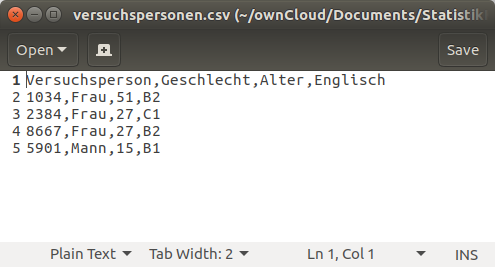
\includegraphics[max width = 0.6\textwidth]{figs/csv.png}
\caption{Ein Datensatz, der als \textit{comma-separated values} gespeichert ist.}
\label{fig:csv}
\end{figure}

In Excel ist es blöderweise eher schwierig, Datensätze im CSV-Format zu speichern:
Zwar gibt es diese Option, aber auf deutsch- oder französischsprachigen Systemen
werden statt Kommas Semikolonen als Trennzeichen verwendet.
In LibreOffice.org hingegen wird man jedes Mal gefragt, ob man Kommas oder Semikolonen
verwenden will.

Manchmal werden Texteinträge auch noch zwischen Anführungszeichen gestellt, sodass
Kommas auch in einem Textfeld vorkommen können. Die folgenden Funktionen erkennen
dies in der Regel automatisch.\footnote{Wenn Sie vorher schon mit R gearbeitet haben, ist die Wahrscheinlichkeit gross, dass Sie statt der \texttt{read\_csv()}-Funktion (mit \texttt{\_}) die \texttt{read.csv()}-Funktion (mit \texttt{.}) verwendet haben.
\texttt{read.csv()} ist die Einlesefunktion von \textit{base R};
\texttt{read\_csv()} ist ihre Entsprechung aus dem \textit{tidyverse}.}
Die \texttt{read\_csv()}-Funktion gehört zum \texttt{readr}-Package,
das automatisch geladen wird, wenn das \texttt{tidyverse}-Bündel geladen wird.

\begin{knitrout}
\definecolor{shadecolor}{rgb}{0.969, 0.969, 0.969}\color{fgcolor}\begin{kframe}
\begin{alltt}
\hlstd{> }\hlstd{participants} \hlkwb{<-} \hlkwd{read_csv}\hlstd{(}\hlkwd{here}\hlstd{(}\hlstr{"data"}\hlstd{,} \hlstr{"versuchspersonen.csv"}\hlstd{))}
\end{alltt}


{\ttfamily\noindent\itshape\color{messagecolor}{Rows: 4 Columns: 4\\-- Column specification ------------------------------------\\Delimiter: "{},"{}\\chr (2): Geschlecht, Englisch\\dbl (2): Versuchsperson, Alter

i Use `spec()` to retrieve the full column specification for this data.\\i Specify the column types or set `show\_col\_types = FALSE` to quiet this message.}}\end{kframe}
\end{knitrout}

Beim Ausführen dieser Befehle werden ein paar Mitteilungen (keine Fehlermeldungen!)
angezeigt, die unter anderem zeigen, dass die \texttt{read\_csv()}-Funktion erkannt hat,
dass in den Spalten \texttt{Versuchsperson} und \texttt{Alter} nur Zahlen stehen (`dbl' für `double', ein Zahlenformat)
und in den Spalten \texttt{Geschlecht} und \texttt{Englisch} auch Buchstaben (`chr' für `character').
Lesen Sie nun noch den Datensatz mit den zu übersetzenden Wörtern ein; die Mitteilungen,
die Sie in der R-Konsole beim Ausführen solcher Befehle sehen werden,
werden in diesem Skript nicht mehr angezeigt.
\begin{knitrout}
\definecolor{shadecolor}{rgb}{0.969, 0.969, 0.969}\color{fgcolor}\begin{kframe}
\begin{alltt}
\hlstd{> }\hlstd{items} \hlkwb{<-} \hlkwd{read_csv}\hlstd{(}\hlkwd{here}\hlstd{(}\hlstr{"data"}\hlstd{,} \hlstr{"woerter.csv"}\hlstd{))}
\end{alltt}


{\ttfamily\noindent\itshape\color{messagecolor}{Rows: 5 Columns: 2\\-- Column specification ------------------------------------\\Delimiter: "{},"{}\\chr (2): Wort, RichtigeÜbersetzung

i Use `spec()` to retrieve the full column specification for this data.\\i Specify the column types or set `show\_col\_types = FALSE` to quiet this message.}}\end{kframe}
\end{knitrout}

\paragraph{Aufgabe.} Inspizieren Sie die beiden Datensätze \texttt{participants}
und \texttt{items}.

\begin{framed}
\noindent \textbf{Einschub: Unterschiedliche CSV-Formate.} Wenn Sie auf einem französisch- oder
deutschsprachigen Computersystem in Excel ein Spread\-sheet im `CSV-Format' speichern,
werden die unterschiedlichen Zellen nicht mit Kommas sondern mit Semikolonen voneinander
getrennt. Der Grund ist, dass das Komma in diesen Sprachen als Dezimaltrennzeichen dient
und daher nicht mehr zur Trennung von Zellen verwendet werden kann. `CSV'-Dateien, in
denen Zellen durch Semikolonen getrennt werden, können Sie in R einlesen, indem Sie statt
der Funktion \texttt{read\_csv()} die Funktion \texttt{read\_csv2()} verwenden.

In LibreOffice.org kann man für jede Datei selber einstellen,
ob Kommas oder Semikolonen zur Trennung von Zellen verwendet werden sollten,
und welches Symbol als Dezimaltrennzeichen dienen soll.
\end{framed}

\section{Datensätze zusammenfügen}\label{sec:join}
Wir haben nun drei Datensätze eingelesen: 
einen mit den Antworten in der Übersetzungsaufgabe
(\texttt{translations}),
einen mit Informationen zu den zu übersetzenden Wörtern
(\texttt{items}),
und einen mit Informationen zu den Teilnehmenden
(\texttt{participants}).
Um die Daten auszuwerten, müssten diese Datensätze miteinander verknüpft werden.
Zum Beispiel müssten wir dem Datensatz \texttt{translations} 
drei Spalten mit Informationen zu den jeweiligen Versuchspersonen hinzufügen:
\texttt{Geschlecht}, \texttt{Alter}, \texttt{Englisch}.
Für Zeilen in \texttt{translations},
für die \texttt{Versuchsperson} \texttt{1034} ist, 
sind die Einträge also \texttt{Frau}, \texttt{51} respektive \texttt{B2};
ist \texttt{Versuchsperson} = \texttt{5901},
sind die Einträge \texttt{Mann}, \texttt{15} respektive \texttt{B1}.
Wenn die gemeinsame Spalte in den beiden Datensätzen identisch heisst,
ist dies ein Kinderspiel:
\begin{knitrout}
\definecolor{shadecolor}{rgb}{0.969, 0.969, 0.969}\color{fgcolor}\begin{kframe}
\begin{alltt}
\hlstd{> }\hlstd{all_data} \hlkwb{<-} \hlkwd{left_join}\hlstd{(}\hlkwc{x} \hlstd{= translations,} \hlkwc{y} \hlstd{= participants)}
\end{alltt}


{\ttfamily\noindent\itshape\color{messagecolor}{Joining, by = "{}Versuchsperson"{}}}\end{kframe}
\end{knitrout}

\paragraph{Aufgabe.} Verwenden Sie die \texttt{View()}-Funktion,
um \texttt{all\_data} zu inspizieren.

Die \texttt{left\_join()}-Funktion erkennt, dass es in beiden Datensätzen
eine Spalte \texttt{Versuchsperson} gibt und
verwendet diese als `Reissverschluss'. Wenn die Funktion
Schwierigkeiten hat, zu erkennen, welche Variable oder welche
Variablen sie als Reissverschluss nehmen soll, kann man diese auch
explizit einstellen:
\begin{knitrout}
\definecolor{shadecolor}{rgb}{0.969, 0.969, 0.969}\color{fgcolor}\begin{kframe}
\begin{alltt}
\hlstd{> }\hlstd{all_data} \hlkwb{<-} \hlkwd{left_join}\hlstd{(}\hlkwc{x} \hlstd{= translations,} \hlkwc{y} \hlstd{= participants,}
\hlstd{+ }                      \hlkwc{by} \hlstd{=} \hlstr{"Versuchsperson"}\hlstd{)}
\end{alltt}
\end{kframe}
\end{knitrout}

Um auch noch Informationen zu den zu übersetzenden Wörtern
hinzuzufügen, wiederholen wir den Befehl mit \texttt{y = items}.
Das Ergebnis dieser Aktion sollten Sie wiederum selber inspizieren.
\begin{knitrout}
\definecolor{shadecolor}{rgb}{0.969, 0.969, 0.969}\color{fgcolor}\begin{kframe}
\begin{alltt}
\hlstd{> }\hlstd{all_data} \hlkwb{<-} \hlkwd{left_join}\hlstd{(}\hlkwc{x} \hlstd{= all_data,} \hlkwc{y} \hlstd{= items,} \hlkwc{by} \hlstd{=} \hlstr{"Wort"}\hlstd{)}
\end{alltt}
\end{kframe}
\end{knitrout}

Die \texttt{left\_join()}-Funktion bewirkt, dass alle Einträge
in Datensatz \texttt{x} bewahrt bleiben und diesem Datensatz die entsprechenden
Informationen aus Datensatz \texttt{y} hinzugefügt werden, insofern welche vorhanden sind.
Wenn es keine Entsprechung in \texttt{y} gibt, erscheint in den hinzugefügten Spalten \texttt{NA}.
Weitere `join'-Funktionen sind die folgenden; siehe \url{https://dplyr.tidyverse.org/reference/join.html} für Details:

\begin{itemize}
 \item \texttt{right\_join()}: Alle Einträge aus Datensatz \texttt{y} bleiben bewahrt; Entsprechungen aus \texttt{x} werden hinzugefügt, falls vorhanden.
 \item \texttt{full\_join()}: Alle Einträge aus beiden Datensätzen bleiben bewahrt. \texttt{NA}, falls es im jeweils anderen Datensatz keine Entsprechung gibt.
 \item \texttt{inner\_join()}: Nur Einträge aus Datensatz \texttt{x}, für die es eine Entsprechung in \texttt{y} gibt, bleiben bewahrt. Diese Entsprechungen werden hinzugefügt.
 \item \texttt{semi\_join()}: Nur Einträge aus Datensatz \texttt{x}, für die es eine Entsprechung in \texttt{y} gibt, bleiben bewahrt. Diese Entsprechungen werden nicht hinzugefügt.
 \item \texttt{anti\_join()}: Nur Einträge aus Datensatz \texttt{x}, für die es keine Entsprechung in \texttt{y} gibt, bleiben bewahrt.
\end{itemize}

In diesem Beispiel würden \texttt{left\_join()}, \texttt{right\_join()}, \texttt{full\_join()}
und \texttt{inner\_join()} zum gleichen Resultat führen, aber dies ist nicht immer der Fall. Siehe hierzu die Übungen am Ende dieses Kapitels.

\section{Informationen abfragen}
Wir wissen bereits, dass wir mit \texttt{View()} einen
ganzen \textit{tibble} oder \textit{data frame} (siehe Fussnote
\ref{fn:tibble}) inspizieren kann. Um diese
auf der Konsole zu zeigen, kann man stattdessen auch einfach
den Namen des Objekts eintippen. Wenn der Datensatz zu gross ist,
werden dann aber nur einige Zeilen und Spalten gezeigt:

\begin{knitrout}
\definecolor{shadecolor}{rgb}{0.969, 0.969, 0.969}\color{fgcolor}\begin{kframe}
\begin{alltt}
\hlstd{> }\hlstd{all_data}
\end{alltt}
\begin{verbatim}
# A tibble: 20 x 9
  Versuchsperson Position Wort      Übersetzung Richtig
           <dbl>    <dbl> <chr>     <chr>         <dbl>
1           1034        1 söka      Socken            0
2           1034        2 försiktig vorsichtig        1
3           1034        3 mjölk     Milch             1
4           1034        4 behärska  <NA>              0
5           1034        5 fiende    finden            0
6           2384        1 fiende    <NA>              0
7           2384        2 behärska  <NA>              0
# ... with 13 more rows, and 4 more variables:
#   Geschlecht <chr>, Alter <dbl>, Englisch <chr>,
#   RichtigeÜbersetzung <chr>
\end{verbatim}
\end{kframe}
\end{knitrout}

Bei grösseren Datensätzen wird es natürlich auch schwieriger,
spezifische Informationen im Datensatz selber nachzuschlagen.
Im Folgenden werden daher einige Techniken vorgestellt, um
die Suche zu erleichtern.

\subsection{Zeilen nach Zeilennummer auswählen}
Mit diesem Befehl zeigen wir die dritte Zeile des Datensatzes
\texttt{all\_data} an. Am Datensatz ändert sich hierdurch nichts. 
Wir verlieren die anderen 19 Zeilen also nicht.
\begin{knitrout}
\definecolor{shadecolor}{rgb}{0.969, 0.969, 0.969}\color{fgcolor}\begin{kframe}
\begin{alltt}
\hlstd{> }\hlkwd{slice}\hlstd{(all_data,} \hlnum{3}\hlstd{)}
\end{alltt}
\begin{verbatim}
# A tibble: 1 x 9
  Versuchsperson Position Wort  Übersetzung Richtig
           <dbl>    <dbl> <chr> <chr>         <dbl>
1           1034        3 mjölk Milch             1
# ... with 4 more variables: Geschlecht <chr>, Alter <dbl>,
#   Englisch <chr>, RichtigeÜbersetzung <chr>
\end{verbatim}
\end{kframe}
\end{knitrout}

Eine alternative Schreibweise ist die folgende. 
Mit der Symbolenfolge \texttt{|>} wird das Objekt vor ihr
(hier: \texttt{all\_data}) der Funktion nach ihr 
als erster Funktionsparameter übergeben:
\begin{knitrout}
\definecolor{shadecolor}{rgb}{0.969, 0.969, 0.969}\color{fgcolor}\begin{kframe}
\begin{alltt}
\hlstd{> }\hlstd{all_data |>}
\hlstd{+ }  \hlkwd{slice}\hlstd{(}\hlnum{3}\hlstd{)}
\end{alltt}
\begin{verbatim}
# A tibble: 1 x 9
  Versuchsperson Position Wort  Übersetzung Richtig
           <dbl>    <dbl> <chr> <chr>         <dbl>
1           1034        3 mjölk Milch             1
# ... with 4 more variables: Geschlecht <chr>, Alter <dbl>,
#   Englisch <chr>, RichtigeÜbersetzung <chr>
\end{verbatim}
\end{kframe}
\end{knitrout}

\medskip

\begin{framed}
\noindent \textbf{Einschub: |>?} 
Die Symbolenfolge \texttt{|>} wird \textit{pipe} genannt und
wird verwendet,
um Befehle übersichtlicher zu organisieren.
Sie wird als \textit{dann} (\textit{then}) ausgesprochen.
Für einfache Befehle wie diesen gibt es eigentlich keinen Mehrwert.
Aber sobald wir mehrere Befehle kombinieren, ist die Notation mit
\textit{pipes} wesentlich einfacher zu lesen und zu verstehen.

Kürzel in RStudio: \textsc{ctrl} + \textsc{shift} + \textsc{m}.
\end{framed}

Im Folgenden werden die Ergebnisse der Befehle nicht mehr angezeigt.
Probieren Sie die Befehle aber dennoch aus.
Bemerken Sie die Verwendung von \texttt{c()} (für `combine')
sowie von \texttt{:}. Auch können mehrere Befehle verkettet werden.
\begin{knitrout}
\definecolor{shadecolor}{rgb}{0.969, 0.969, 0.969}\color{fgcolor}\begin{kframe}
\begin{alltt}
\hlstd{> }\hlcom{# Zeilen 5 und 7 auswählen.}
\hlstd{> }\hlstd{all_data |>}
\hlstd{+ }  \hlkwd{slice}\hlstd{(}\hlkwd{c}\hlstd{(}\hlnum{5}\hlstd{,} \hlnum{7}\hlstd{))}
\hlstd{> }
\hlstd{> }\hlcom{# Zeilen 5 bis 7 einschliesslich auswählen}
\hlstd{> }\hlstd{all_data |>}
\hlstd{+ }  \hlkwd{slice}\hlstd{(}\hlnum{5}\hlopt{:}\hlnum{7}\hlstd{)}
\hlstd{> }
\hlstd{> }\hlcom{# Zeilen 5 bis 7 auswählen, dann vollständig zeigen}
\hlstd{> }\hlstd{all_data |>}
\hlstd{+ }  \hlkwd{slice}\hlstd{(}\hlnum{5}\hlopt{:}\hlnum{7}\hlstd{) |>}
\hlstd{+ }  \hlkwd{View}\hlstd{()}
\end{alltt}
\end{kframe}
\end{knitrout}

Mit den obigen Befehlen werden nur gewisse Zeilen in der Konsole angezeigt.
Man kann den Output stattdessen auch als neues Objekt speichern:
\begin{knitrout}
\definecolor{shadecolor}{rgb}{0.969, 0.969, 0.969}\color{fgcolor}\begin{kframe}
\begin{alltt}
\hlstd{> }\hlstd{zeilen7_12} \hlkwb{<-} \hlstd{all_data |>}
\hlstd{+ }  \hlkwd{slice}\hlstd{(}\hlnum{7}\hlopt{:}\hlnum{12}\hlstd{)}
\end{alltt}
\end{kframe}
\end{knitrout}

Jetzt werden die Zeilen nicht angezeigt, aber sie sind fortan verfügbar als neues Objekt
im Arbeitsspeicher. Um dieses Objekt zu inspizieren, können Sie seinen Namen eintippen
oder \texttt{View} verwenden:
\begin{knitrout}
\definecolor{shadecolor}{rgb}{0.969, 0.969, 0.969}\color{fgcolor}\begin{kframe}
\begin{alltt}
\hlstd{> }\hlstd{zeilen7_12}
\end{alltt}
\begin{verbatim}
# A tibble: 6 x 9
  Versuchsperson Position Wort      Übersetzung Richtig
           <dbl>    <dbl> <chr>     <chr>         <dbl>
1           2384        2 behärska  <NA>              0
2           2384        3 försiktig vorsichtig        1
3           2384        4 mjölk     Milch             1
4           2384        5 söka      Socke             0
5           8667        1 mjölk     Milch             1
6           8667        2 behärska  <NA>              0
# ... with 4 more variables: Geschlecht <chr>, Alter <dbl>,
#   Englisch <chr>, RichtigeÜbersetzung <chr>
\end{verbatim}
\end{kframe}
\end{knitrout}

\subsection{Zeilen nach bestimmten Werten auswählen}
Mit \texttt{slice()} können wir Zeilen je nach ihrer Position
im Datensatz auswählen. In der Regel wählen wir jedoch die Zeilen
je nach gewissen Eigenschaften dieser Zeilen aus. Dazu verwenden
wir die \texttt{filter()}-Funktion. Beispielsweise können
wir nur jene Zeilen, die das Wort \texttt{fiende} betreffen auswählen.
Bemerken Sie, dass die Zeichenkombination \texttt{==} verwendet wird,
um auf Gleichheit zu testen:
\begin{knitrout}
\definecolor{shadecolor}{rgb}{0.969, 0.969, 0.969}\color{fgcolor}\begin{kframe}
\begin{alltt}
\hlstd{> }\hlstd{all_data |>}
\hlstd{+ }  \hlkwd{filter}\hlstd{(Wort} \hlopt{==} \hlstr{"fiende"}\hlstd{)}
\end{alltt}
\begin{verbatim}
# A tibble: 4 x 9
  Versuchsperson Position Wort   Übersetzung Richtig
           <dbl>    <dbl> <chr>  <chr>         <dbl>
1           1034        5 fiende finden            0
2           2384        1 fiende <NA>              0
3           8667        3 fiende finden            0
4           5901        4 fiende feinde            1
# ... with 4 more variables: Geschlecht <chr>, Alter <dbl>,
#   Englisch <chr>, RichtigeÜbersetzung <chr>
\end{verbatim}
\end{kframe}
\end{knitrout}

Um nur die Zeilen auszuwählen, die nicht das Wort \texttt{fiende}
betreffen, kann man \texttt{==} durch \texttt{!=} ersetzen.

Wir können auch jene Zeilen auswählen, die Versuchspersonen
mit einem Alter über 30 betreffen:
\begin{knitrout}
\definecolor{shadecolor}{rgb}{0.969, 0.969, 0.969}\color{fgcolor}\begin{kframe}
\begin{alltt}
\hlstd{> }\hlstd{all_data |>}
\hlstd{+ }  \hlkwd{filter}\hlstd{(Alter} \hlopt{>} \hlnum{30}\hlstd{)}
\end{alltt}
\begin{verbatim}
# A tibble: 5 x 9
  Versuchsperson Position Wort      Übersetzung Richtig
           <dbl>    <dbl> <chr>     <chr>         <dbl>
1           1034        1 söka      Socken            0
2           1034        2 försiktig vorsichtig        1
3           1034        3 mjölk     Milch             1
4           1034        4 behärska  <NA>              0
5           1034        5 fiende    finden            0
# ... with 4 more variables: Geschlecht <chr>, Alter <dbl>,
#   Englisch <chr>, RichtigeÜbersetzung <chr>
\end{verbatim}
\end{kframe}
\end{knitrout}
Für Versuchpersonen unter 30 würde man \texttt{<} verwenden;
für Versuchspersonen unter 30 einschliesslich \texttt{<=}.

Wir können auch nur jene Zeilen beibehalten, für die
keine Übersetzung (also mit \texttt{NA} als Übersetzung)
gegeben wurde. Dann verwendet man aber am besten die Hilfefunktion
\texttt{is.na()}:
\begin{knitrout}
\definecolor{shadecolor}{rgb}{0.969, 0.969, 0.969}\color{fgcolor}\begin{kframe}
\begin{alltt}
\hlstd{> }\hlstd{all_data |>}
\hlstd{+ }  \hlkwd{filter}\hlstd{(}\hlkwd{is.na}\hlstd{(Übersetzung))}
\end{alltt}
\begin{verbatim}
# A tibble: 4 x 9
  Versuchsperson Position Wort     Übersetzung Richtig
           <dbl>    <dbl> <chr>    <chr>         <dbl>
1           1034        4 behärska <NA>              0
2           2384        1 fiende   <NA>              0
3           2384        2 behärska <NA>              0
4           8667        2 behärska <NA>              0
# ... with 4 more variables: Geschlecht <chr>, Alter <dbl>,
#   Englisch <chr>, RichtigeÜbersetzung <chr>
\end{verbatim}
\end{kframe}
\end{knitrout}

Mit \texttt{!is.na()} selektieren wir dann wieder nur jene Zeilen,
wo die Übersetzung nicht fehlt:
\begin{knitrout}
\definecolor{shadecolor}{rgb}{0.969, 0.969, 0.969}\color{fgcolor}\begin{kframe}
\begin{alltt}
\hlstd{> }\hlstd{all_data |>}
\hlstd{+ }  \hlkwd{filter}\hlstd{(}\hlopt{!}\hlkwd{is.na}\hlstd{(Übersetzung))}
\end{alltt}
\begin{verbatim}
# A tibble: 16 x 9
  Versuchsperson Position Wort      Übersetzung Richtig
           <dbl>    <dbl> <chr>     <chr>         <dbl>
1           1034        1 söka      Socken            0
2           1034        2 försiktig vorsichtig        1
3           1034        3 mjölk     Milch             1
4           1034        5 fiende    finden            0
5           2384        3 försiktig vorsichtig        1
6           2384        4 mjölk     Milch             1
7           2384        5 söka      Socke             0
# ... with 9 more rows, and 4 more variables:
#   Geschlecht <chr>, Alter <dbl>, Englisch <chr>,
#   RichtigeÜbersetzung <chr>
\end{verbatim}
\end{kframe}
\end{knitrout}

Wir können auch mehrere \texttt{filter()}-Befehle verketten.
Beispielsweise können wir aus dem Datensatz jene Zeilen auslesen,
für die Position gleich 1 ist und für die eine falsche Antwort gegeben wurde:
\begin{knitrout}
\definecolor{shadecolor}{rgb}{0.969, 0.969, 0.969}\color{fgcolor}\begin{kframe}
\begin{alltt}
\hlstd{> }\hlstd{all_data |>}
\hlstd{+ }  \hlkwd{filter}\hlstd{(Position} \hlopt{==} \hlnum{1}\hlstd{) |>}
\hlstd{+ }  \hlkwd{filter}\hlstd{(Richtig} \hlopt{==} \hlnum{0}\hlstd{)}
\end{alltt}
\begin{verbatim}
# A tibble: 2 x 9
  Versuchsperson Position Wort   Übersetzung Richtig
           <dbl>    <dbl> <chr>  <chr>         <dbl>
1           1034        1 söka   Socken            0
2           2384        1 fiende <NA>              0
# ... with 4 more variables: Geschlecht <chr>, Alter <dbl>,
#   Englisch <chr>, RichtigeÜbersetzung <chr>
\end{verbatim}
\end{kframe}
\end{knitrout}
Eine Alternative ist diese:
\begin{knitrout}
\definecolor{shadecolor}{rgb}{0.969, 0.969, 0.969}\color{fgcolor}\begin{kframe}
\begin{alltt}
\hlstd{> }\hlcom{# Output nicht im Skript}
\hlstd{> }\hlstd{all_data |>}
\hlstd{+ }  \hlkwd{filter}\hlstd{(Position} \hlopt{==} \hlnum{1} \hlopt{&} \hlstd{Richtig} \hlopt{==} \hlnum{0}\hlstd{)}
\end{alltt}
\end{kframe}
\end{knitrout}
Wollen wir die Zeilen auslesen, für die Position gleich 1 ist oder
für die eine falsche Antwort gegeben wurde, so verwenden wir diesen Befehl:
\begin{knitrout}
\definecolor{shadecolor}{rgb}{0.969, 0.969, 0.969}\color{fgcolor}\begin{kframe}
\begin{alltt}
\hlstd{> }\hlcom{# Output nicht im Skript}
\hlstd{> }\hlstd{all_data |>}
\hlstd{+ }  \hlkwd{filter}\hlstd{(Position} \hlopt{==} \hlnum{1} \hlopt{|} \hlstd{Richtig} \hlopt{==} \hlnum{0}\hlstd{)}
\end{alltt}
\end{kframe}
\end{knitrout}


Die Ergebnisse all dieser Auswählaktionen
können auch als separate Objekte gespeichert und angezeigt werden.
\begin{knitrout}
\definecolor{shadecolor}{rgb}{0.969, 0.969, 0.969}\color{fgcolor}\begin{kframe}
\begin{alltt}
\hlstd{> }\hlstd{nur_fiende} \hlkwb{<-} \hlstd{all_data |>}
\hlstd{+ }  \hlkwd{filter}\hlstd{(Wort} \hlopt{==} \hlstr{"fiende"}\hlstd{)}
\hlstd{> }
\hlstd{> }\hlstd{nur_fiende}
\end{alltt}
\begin{verbatim}
# A tibble: 4 x 9
  Versuchsperson Position Wort   Übersetzung Richtig
           <dbl>    <dbl> <chr>  <chr>         <dbl>
1           1034        5 fiende finden            0
2           2384        1 fiende <NA>              0
3           8667        3 fiende finden            0
4           5901        4 fiende feinde            1
# ... with 4 more variables: Geschlecht <chr>, Alter <dbl>,
#   Englisch <chr>, RichtigeÜbersetzung <chr>
\end{verbatim}
\end{kframe}
\end{knitrout}

\subsection{Spalten auswählen}
Manchmal enthält ein Datensatz schlicht zu viele Spalten, die
für die aktuelle Analyse nicht relevant sind. Mit \texttt{select()}
können wir die Spalten auswählen, die wir gerade brauchen:\footnote{Für diejenigen unter Ihnen mit SQL-Erfahrung: Beachten Sie, dass
der SQL-Befehl \texttt{SELECT} nicht dem R-Befehl \texttt{select()}, sondern \texttt{filter()} entspricht.}
\begin{knitrout}
\definecolor{shadecolor}{rgb}{0.969, 0.969, 0.969}\color{fgcolor}\begin{kframe}
\begin{alltt}
\hlstd{> }\hlstd{all_data |>}
\hlstd{+ }  \hlkwd{select}\hlstd{(Wort, RichtigeÜbersetzung, Übersetzung) |>}
\hlstd{+ }  \hlkwd{slice_head}\hlstd{(}\hlkwc{n} \hlstd{=} \hlnum{5}\hlstd{)}
\end{alltt}
\begin{verbatim}
# A tibble: 5 x 3
  Wort      RichtigeÜbersetzung Übersetzung
  <chr>     <chr>               <chr>      
1 söka      suchen              Socken     
2 försiktig vorsichtig          vorsichtig 
3 mjölk     milch               Milch      
4 behärska  beherrschen         <NA>       
5 fiende    Feind               finden     
\end{verbatim}
\end{kframe}
\end{knitrout}

Es gibt auch ein paar Hilfefunktionen,
mit denen man effizienter Spalten auswählen kann.
Diese sind insbesondere bei grossen Datensätzen nützlich.
Beispiele sind \texttt{contains()} und \texttt{starts\_with()}.
\begin{knitrout}
\definecolor{shadecolor}{rgb}{0.969, 0.969, 0.969}\color{fgcolor}\begin{kframe}
\begin{alltt}
\hlstd{> }\hlstd{all_data |>}
\hlstd{+ }  \hlkwd{select}\hlstd{(}\hlkwd{contains}\hlstd{(}\hlstr{"Übersetzung"}\hlstd{)) |>}
\hlstd{+ }  \hlkwd{slice}\hlstd{(}\hlnum{5}\hlopt{:}\hlnum{7}\hlstd{)}
\end{alltt}
\begin{verbatim}
# A tibble: 3 x 2
  Übersetzung RichtigeÜbersetzung
  <chr>       <chr>              
1 finden      Feind              
2 <NA>        Feind              
3 <NA>        beherrschen        
\end{verbatim}
\begin{alltt}
\hlstd{> }\hlstd{all_data |>}
\hlstd{+ }  \hlkwd{select}\hlstd{(}\hlkwd{starts_with}\hlstd{(}\hlstr{"Richt"}\hlstd{)) |>}
\hlstd{+ }  \hlkwd{slice_tail}\hlstd{(}\hlkwc{n} \hlstd{=} \hlnum{4}\hlstd{)}
\end{alltt}
\begin{verbatim}
# A tibble: 4 x 2
  Richtig RichtigeÜbersetzung
    <dbl> <chr>              
1       1 milch              
2       1 vorsichtig         
3       1 Feind              
4       0 suchen             
\end{verbatim}
\end{kframe}
\end{knitrout}

Für weitere Hilfefunktionen,
siehe \url{https://tidyselect.r-lib.org}.

\subsection{Weitere Beispiele}
Die unterschiedlichen Befehle können verkettet werden.
So können wir nur die Übersetzungen fürs Wort \texttt{fiende}
abrufen:
\begin{knitrout}
\definecolor{shadecolor}{rgb}{0.969, 0.969, 0.969}\color{fgcolor}\begin{kframe}
\begin{alltt}
\hlstd{> }\hlstd{all_data |>}
\hlstd{+ }  \hlkwd{filter}\hlstd{(Wort} \hlopt{==} \hlstr{"fiende"}\hlstd{) |>}
\hlstd{+ }  \hlkwd{select}\hlstd{(Übersetzung)}
\end{alltt}
\begin{verbatim}
# A tibble: 4 x 1
  Übersetzung
  <chr>      
1 finden     
2 <NA>       
3 finden     
4 feinde     
\end{verbatim}
\end{kframe}
\end{knitrout}

Oder wir können mit \texttt{distinct()} auch nur die unterschiedlichen Übersetzungen
fürs Wort \texttt{behärska} abrufen:
\begin{knitrout}
\definecolor{shadecolor}{rgb}{0.969, 0.969, 0.969}\color{fgcolor}\begin{kframe}
\begin{alltt}
\hlstd{> }\hlstd{all_data |>}
\hlstd{+ }  \hlkwd{filter}\hlstd{(Wort} \hlopt{==} \hlstr{"behärska"}\hlstd{) |>}
\hlstd{+ }  \hlkwd{select}\hlstd{(Übersetzung) |>}
\hlstd{+ }  \hlkwd{distinct}\hlstd{()}
\end{alltt}
\begin{verbatim}
# A tibble: 2 x 1
  Übersetzung
  <chr>      
1 <NA>       
2 beherrschen
\end{verbatim}
\end{kframe}
\end{knitrout}

Führen Sie auch einmal diesen Befehl ohne \texttt{distinct()} aus.
Im letzten Beispiel wird auch langsam klar, wieso es sich lohnt,
das \textit{pipe} (\texttt{|>}) zu verwenden. Ohne sähe
diese Befehlenkombination nämlich so aus:
\begin{knitrout}
\definecolor{shadecolor}{rgb}{0.969, 0.969, 0.969}\color{fgcolor}\begin{kframe}
\begin{alltt}
\hlstd{> }\hlkwd{distinct}\hlstd{(}\hlkwd{select}\hlstd{(}\hlkwd{filter}\hlstd{(all_data, Wort} \hlopt{==} \hlstr{"behärska"}\hlstd{), Übersetzung))}
\end{alltt}
\end{kframe}
\end{knitrout}

\texttt{filter()} ist der Befehl,
der zuerst ausgeführt werden muss,
aber in dieser Notation wird er als letzter geschrieben.
Mit der pipe-Notation schreibt man die Befehle in der
Reihenfolge, in der sie ausgeführt werden müssen.

\section{Datensätze umgestalten}\label{sec:pivot}
Die meiste Zeit, die man sich für die Analyse eines Datensatzes
reserviert, verbringt man oft nicht mit Berechnungen und mit dem Modellieren,
sondern mit sog.\ \textit{data wrangling}: Man muss zunächst einmal
dafür sorgen, dass der Datensatz in einem Format vorliegt, in dem er
analysiert werden kann. Data wrangling eignet sich wohl am besten
für \textit{learning by doing}. Eine Technik, die man aber oft braucht,
ist das Konvertieren zwischen langen bzw.\ längeren und breiten bzw.\ breiteren
Formaten. Diese Technik soll hier illustriert werden anhand eines Datensatzes
zu einer Längsschnittstudie zur Entwicklung von Lese- und Schreibfähigkeiten
bei Portugiesisch--Französisch- und Portugiesisch--Deutsch-Zwei\-sprachigen
\citep{Lambelet_HELASCOT_writing,Pestana_HELASCOT_reading}.

\paragraph{Aufgabe.} Lesen Sie den Datensatz \texttt{helascot\_skills.csv} als \texttt{skills} ein
und inspizieren Sie seine Struktur.\label{page:skills}



Sie werden bemerken, dass pro Versuchsperson
(\texttt{Subject}) pro Zeitpunkt und pro getestete Sprache drei Messungen
vorliegen: \texttt{Reading}, \texttt{Argumentation} und \texttt{Narration}.
Wir können diesen Datensatz länger machen, indem wir diese Messungen unter- statt
nebeneinander stellen. Hierzu verwenden wir die Funktion \texttt{pivot\_longer()}.
Die drei Spalten, die wir dem Parameter \texttt{cols} übergeben, werden nun
untereinander gestellt; die neue Spalte \texttt{Skill} gibt an, aus welcher
Spalte die Messungen stammen; die neue Spalte \texttt{Score} enthält die
Werte, die in den drei ursprünglichen Spalten standen.

\begin{knitrout}
\definecolor{shadecolor}{rgb}{0.969, 0.969, 0.969}\color{fgcolor}\begin{kframe}
\begin{alltt}
\hlstd{> }\hlstd{skills_longer} \hlkwb{<-} \hlstd{skills |>}
\hlstd{+ }  \hlkwd{pivot_longer}\hlstd{(}\hlkwc{cols} \hlstd{=} \hlkwd{c}\hlstd{(}\hlstr{"Reading"}\hlstd{,} \hlstr{"Argumentation"}\hlstd{,} \hlstr{"Narration"}\hlstd{),}
\hlstd{+ }               \hlkwc{names_to} \hlstd{=} \hlstr{"Skill"}\hlstd{,}
\hlstd{+ }               \hlkwc{values_to} \hlstd{=} \hlstr{"Score"}\hlstd{)}
\hlstd{> }\hlstd{skills_longer}
\end{alltt}
\begin{verbatim}
# A tibble: 5,712 x 5
  Subject  Time LanguageTested Skill          Score
  <chr>   <dbl> <chr>          <chr>          <dbl>
1 A_PLF_1     1 French         Reading        0.211
2 A_PLF_1     1 French         Argumentation  7    
3 A_PLF_1     1 French         Narration     NA    
4 A_PLF_1     1 Portuguese     Reading        0.579
5 A_PLF_1     1 Portuguese     Argumentation  9    
6 A_PLF_1     1 Portuguese     Narration      6    
7 A_PLF_1     2 French         Reading        0.684
# ... with 5,705 more rows
\end{verbatim}
\end{kframe}
\end{knitrout}

Jetzt, wo die Daten in diesem noch längeren Format vorliegen,
können wir den Datensatz zu einem breiteren Format umgestalten,
wo aber die Angaben zu den unterschiedlichen Zeitpunkten
(statt zu den unterschiedlichen Fähigkeiten) nebeneinander stehen.
Hierzu verwenden wir die Funktion \texttt{pivot\_wider()}.
Da die Werte in der Spalte \texttt{Time} numerisch sind, fügen
wir ihnen mit dem Parameter \texttt{names\_prefix} noch ein \texttt{T} hinzu:

\begin{knitrout}
\definecolor{shadecolor}{rgb}{0.969, 0.969, 0.969}\color{fgcolor}\begin{kframe}
\begin{alltt}
\hlstd{> }\hlstd{skills_wider_time} \hlkwb{<-} \hlstd{skills_longer |>}
\hlstd{+ }  \hlkwd{pivot_wider}\hlstd{(}\hlkwc{names_from} \hlstd{=} \hlstr{"Time"}\hlstd{,}
\hlstd{+ }              \hlkwc{names_prefix} \hlstd{=} \hlstr{"T"}\hlstd{,}
\hlstd{+ }              \hlkwc{values_from} \hlstd{=} \hlstr{"Score"}\hlstd{)}
\hlstd{> }\hlstd{skills_wider_time}
\end{alltt}
\begin{verbatim}
# A tibble: 2,100 x 6
  Subject  LanguageTested Skill             T1     T2     T3
  <chr>    <chr>          <chr>          <dbl>  <dbl>  <dbl>
1 A_PLF_1  French         Reading        0.211  0.684  0.947
2 A_PLF_1  French         Argumentation  7     14     14    
3 A_PLF_1  French         Narration     NA     10      8    
4 A_PLF_1  Portuguese     Reading        0.579  0.737  0.842
5 A_PLF_1  Portuguese     Argumentation  9     13     13    
6 A_PLF_1  Portuguese     Narration      6      9     NA    
7 A_PLF_10 French         Reading        0.579  0.474  0.316
# ... with 2,093 more rows
\end{verbatim}
\end{kframe}
\end{knitrout}

Dieses Format wäre zum Beispiel praktisch, wenn wir die Unterschiede zwischen
den T1-, T2- und T3-Messungen berechnen möchten. Diese können wir mit
dem Befehl \texttt{mutate()} noch hinzufügen:
\begin{knitrout}
\definecolor{shadecolor}{rgb}{0.969, 0.969, 0.969}\color{fgcolor}\begin{kframe}
\begin{alltt}
\hlstd{> }\hlstd{skills_wider_time |>}
\hlstd{+ }  \hlkwd{mutate}\hlstd{(}
\hlstd{+ }    \hlkwc{ProgressT1_T2} \hlstd{= T2} \hlopt{-} \hlstd{T1,}
\hlstd{+ }    \hlkwc{ProgressT3_T2} \hlstd{= T3} \hlopt{-} \hlstd{T2}
\hlstd{+ }  \hlstd{) |>}
\hlstd{+ }  \hlkwd{select}\hlstd{(Subject, LanguageTested, Skill, ProgressT1_T2, ProgressT3_T2)}
\end{alltt}
\begin{verbatim}
# A tibble: 2,100 x 5
  Subject  LanguageTested Skill  ProgressT1_T2 ProgressT3_T2
  <chr>    <chr>          <chr>          <dbl>         <dbl>
1 A_PLF_1  French         Readi~         0.474         0.263
2 A_PLF_1  French         Argum~         7             0    
3 A_PLF_1  French         Narra~        NA            -2    
4 A_PLF_1  Portuguese     Readi~         0.158         0.105
5 A_PLF_1  Portuguese     Argum~         4             0    
6 A_PLF_1  Portuguese     Narra~         3            NA    
7 A_PLF_10 French         Readi~        -0.105        -0.158
# ... with 2,093 more rows
\end{verbatim}
\end{kframe}
\end{knitrout}

Wir könnten auch die Angaben zu den unterschiedlichen Sprachen nebeneinander stellen.
Die ersten Versuchspersonen waren alle Portugiesisch--Französisch-Zwei\-sprachige,
die nicht auf Deutsch getesten wurden. Daher enthält die letzte Spalte scheinbar
nur \texttt{NA} (\textit{not available}), aber mit \texttt{View()} können Sie
sehen, dass diese Angaben für viele Versuchspersonen tatsächlich vorliegen.
\begin{knitrout}
\definecolor{shadecolor}{rgb}{0.969, 0.969, 0.969}\color{fgcolor}\begin{kframe}
\begin{alltt}
\hlstd{> }\hlstd{skills_wider_language} \hlkwb{<-} \hlstd{skills_longer |>}
\hlstd{+ }  \hlkwd{pivot_wider}\hlstd{(}\hlkwc{names_from} \hlstd{=} \hlstr{"LanguageTested"}\hlstd{,}
\hlstd{+ }              \hlkwc{values_from} \hlstd{=} \hlstr{"Score"}\hlstd{)}
\hlstd{> }\hlstd{skills_wider_language}
\end{alltt}
\begin{verbatim}
# A tibble: 3,999 x 6
  Subject  Time Skill         French Portuguese German
  <chr>   <dbl> <chr>          <dbl>      <dbl>  <dbl>
1 A_PLF_1     1 Reading        0.211      0.579     NA
2 A_PLF_1     1 Argumentation  7          9         NA
3 A_PLF_1     1 Narration     NA          6         NA
4 A_PLF_1     2 Reading        0.684      0.737     NA
5 A_PLF_1     2 Argumentation 14         13         NA
6 A_PLF_1     2 Narration     10          9         NA
7 A_PLF_1     3 Reading        0.947      0.842     NA
# ... with 3,992 more rows
\end{verbatim}
\end{kframe}
\end{knitrout}
Dieses Format wäre dann wieder praktischer, wenn wir
pro Versuchsperson die Unterschiede zwischen den
\texttt{French}-, \texttt{Portuguese}- und \texttt{German}-Messungen
zu jedem Zeitpunkt berechnen möchten:
\begin{knitrout}
\definecolor{shadecolor}{rgb}{0.969, 0.969, 0.969}\color{fgcolor}\begin{kframe}
\begin{alltt}
\hlstd{> }\hlstd{skills_wider_language |>}
\hlstd{+ }  \hlkwd{mutate}\hlstd{(}
\hlstd{+ }    \hlkwc{DiffGer_Port} \hlstd{= German} \hlopt{-} \hlstd{Portuguese,}
\hlstd{+ }    \hlkwc{DiffFre_Port} \hlstd{= French} \hlopt{-} \hlstd{Portuguese}
\hlstd{+ }  \hlstd{) |>}
\hlstd{+ }  \hlkwd{select}\hlstd{(Subject, Time, Skill, DiffGer_Port, DiffFre_Port)}
\end{alltt}
\begin{verbatim}
# A tibble: 3,999 x 5
  Subject  Time Skill         DiffGer_Port DiffFre_Port
  <chr>   <dbl> <chr>                <dbl>        <dbl>
1 A_PLF_1     1 Reading                 NA      -0.368 
2 A_PLF_1     1 Argumentation           NA      -2     
3 A_PLF_1     1 Narration               NA      NA     
4 A_PLF_1     2 Reading                 NA      -0.0526
5 A_PLF_1     2 Argumentation           NA       1     
6 A_PLF_1     2 Narration               NA       1     
7 A_PLF_1     3 Reading                 NA       0.105 
# ... with 3,992 more rows
\end{verbatim}
\end{kframe}
\end{knitrout}


Wir können den Datensatz sogar noch breiter machen:
\begin{knitrout}
\definecolor{shadecolor}{rgb}{0.969, 0.969, 0.969}\color{fgcolor}\begin{kframe}
\begin{alltt}
\hlstd{> }\hlstd{skills_wider_time_language} \hlkwb{<-} \hlstd{skills_longer |>}
\hlstd{+ }  \hlkwd{pivot_wider}\hlstd{(}\hlkwc{names_from} \hlstd{=} \hlkwd{c}\hlstd{(}\hlstr{"LanguageTested"}\hlstd{,} \hlstr{"Time"}\hlstd{),}
\hlstd{+ }              \hlkwc{values_from} \hlstd{=} \hlstr{"Score"}\hlstd{)}
\hlstd{> }\hlstd{skills_wider_time_language}
\end{alltt}
\begin{verbatim}
# A tibble: 1,410 x 11
  Subject  Skill French_1 Portuguese_1 French_2 Portuguese_2
  <chr>    <chr>    <dbl>        <dbl>    <dbl>        <dbl>
1 A_PLF_1  Read~    0.211        0.579    0.684        0.737
2 A_PLF_1  Argu~    7            9       14           13    
3 A_PLF_1  Narr~   NA            6       10            9    
4 A_PLF_10 Read~    0.579        0.316    0.474        0.579
5 A_PLF_10 Argu~    5            6       10            7    
6 A_PLF_10 Narr~   10            7        8           NA    
7 A_PLF_12 Read~    0.895       NA        1            0.947
# ... with 1,403 more rows, and 5 more variables:
#   French_3 <dbl>, Portuguese_3 <dbl>, German_1 <dbl>,
#   German_2 <dbl>, German_3 <dbl>
\end{verbatim}
\end{kframe}
\end{knitrout}

Wenn dies nötig wäre, könnten wir diesen breiten Datensatz
wieder zum langen Format konvertieren. Langsam wird der
Code etwas schwieriger (bei \texttt{names\_pattern} wird
ein sog.\ regulärer Ausdruck verwendet) und für diesen Kurs
ist es nicht so wichtig, dass Sie solche schwierigere Fälle
bereits bewältigen können. Vielmehr soll dieser letzte
Codeblock illustrieren, dass solche Konversionen
möglich sind. Wenn man das weiss, kann man auf der Hilfeseite
von \texttt{pivot\_longer()}
(dazu \texttt{?pivot\_longer} eintippen)
nachschauen, wie die Beispiele dort aussehen und diese ans
eigene Problem anpassen.
\begin{knitrout}
\definecolor{shadecolor}{rgb}{0.969, 0.969, 0.969}\color{fgcolor}\begin{kframe}
\begin{alltt}
\hlstd{> }\hlstd{skills_back} \hlkwb{<-} \hlstd{skills_wider_time_language |>}
\hlstd{+ }  \hlkwd{pivot_longer}\hlstd{(}\hlkwc{cols} \hlstd{= French_1}\hlopt{:}\hlstd{German_3,}
\hlstd{+ }               \hlkwc{names_to} \hlstd{=} \hlkwd{c}\hlstd{(}\hlstr{"Language"}\hlstd{,} \hlstr{"Time"}\hlstd{),}
\hlstd{+ }               \hlkwc{names_pattern} \hlstd{=} \hlstr{"(.*)_(.*)"}\hlstd{,}
\hlstd{+ }               \hlkwc{values_to} \hlstd{=} \hlstr{"Score"}\hlstd{)}
\hlstd{> }\hlstd{skills_back}
\end{alltt}
\begin{verbatim}
# A tibble: 12,690 x 5
  Subject Skill   Language   Time   Score
  <chr>   <chr>   <chr>      <chr>  <dbl>
1 A_PLF_1 Reading French     1      0.211
2 A_PLF_1 Reading Portuguese 1      0.579
3 A_PLF_1 Reading French     2      0.684
4 A_PLF_1 Reading Portuguese 2      0.737
5 A_PLF_1 Reading French     3      0.947
6 A_PLF_1 Reading Portuguese 3      0.842
7 A_PLF_1 Reading German     1     NA    
# ... with 12,683 more rows
\end{verbatim}
\end{kframe}
\end{knitrout}
Die Notation \texttt{French\_1:German\_3} selektiert übrigens
alle Spalten zwischen \texttt{French\_1} und \texttt{German\_3} inklusive. 
Eine Alternative für wenn die Spalten nicht schön praktisch 
nebeneinander stehen, ist diese:
\begin{knitrout}
\definecolor{shadecolor}{rgb}{0.969, 0.969, 0.969}\color{fgcolor}\begin{kframe}
\begin{alltt}
\hlstd{> }\hlstd{skills_back} \hlkwb{<-} \hlstd{skills_wider_time_language |>}
\hlstd{+ }  \hlkwd{pivot_longer}\hlstd{(}\hlkwc{cols} \hlstd{=} \hlkwd{starts_with}\hlstd{(}\hlkwd{c}\hlstd{(}\hlstr{"French"}\hlstd{,} \hlstr{"Portuguese"}\hlstd{,} \hlstr{"German"}\hlstd{)),}
\hlstd{+ }               \hlkwc{names_to} \hlstd{=} \hlkwd{c}\hlstd{(}\hlstr{"Language"}\hlstd{,} \hlstr{"Time"}\hlstd{),}
\hlstd{+ }               \hlkwc{names_pattern} \hlstd{=} \hlstr{"(.*)_(.*)"}\hlstd{,}
\hlstd{+ }               \hlkwc{values_to} \hlstd{=} \hlstr{"Score"}\hlstd{)}
\hlstd{> }\hlstd{skills_back}
\end{alltt}
\begin{verbatim}
# A tibble: 12,690 x 5
  Subject Skill   Language   Time   Score
  <chr>   <chr>   <chr>      <chr>  <dbl>
1 A_PLF_1 Reading French     1      0.211
2 A_PLF_1 Reading French     2      0.684
3 A_PLF_1 Reading French     3      0.947
4 A_PLF_1 Reading Portuguese 1      0.579
5 A_PLF_1 Reading Portuguese 2      0.737
6 A_PLF_1 Reading Portuguese 3      0.842
7 A_PLF_1 Reading German     1     NA    
# ... with 12,683 more rows
\end{verbatim}
\end{kframe}
\end{knitrout}

\section{Zusammenfassungen kreieren}
Die \texttt{summarise()}-Funktion kann man verwenden,
um etwa Durchschnitte von Variablen in einem Datensatz zu berechnen.
So berechnet der nächste Codeblock die Mittel der \texttt{Narration}-
und \texttt{Argumentation}-Variablen im \texttt{skills}-Datensatz.
Bei der \texttt{mean()}-Funktion wird der Parameter \texttt{na.rm}
noch auf \texttt{TRUE} gestellt. Dies bewirkt, dass beim Berechnen
des Mittels fehlende Werte (\texttt{NA}) ignoriert werden; 
andernfalls wären beide Mittel nämlich auch \texttt{NA}.

\begin{knitrout}
\definecolor{shadecolor}{rgb}{0.969, 0.969, 0.969}\color{fgcolor}\begin{kframe}
\begin{alltt}
\hlstd{> }\hlstd{skills |>}
\hlstd{+ }  \hlkwd{summarise}\hlstd{(}\hlkwc{mittel_narr} \hlstd{=} \hlkwd{mean}\hlstd{(Narration,} \hlkwc{na.rm} \hlstd{=} \hlnum{TRUE}\hlstd{),}
\hlstd{+ }            \hlkwc{mittel_arg} \hlstd{=} \hlkwd{mean}\hlstd{(Argumentation,} \hlkwc{na.rm} \hlstd{=} \hlnum{TRUE}\hlstd{))}
\end{alltt}
\begin{verbatim}
# A tibble: 1 x 2
  mittel_narr mittel_arg
        <dbl>      <dbl>
1        8.51       13.0
\end{verbatim}
\end{kframe}
\end{knitrout}

Mit \texttt{group\_by()} können wir solche Zusammenfassungen
auch für durch die Kombinationen der in dieser Funktion
aufgeführten Variablen definierte Untergruppen generieren.
Der Codeblock unten spaltet daher zunächst den Datensatz
\texttt{skills} auf in 9 Untergruppen: eine pro Kombination
der Werte von \texttt{Time} (1, 2, 3) und \texttt{LanguageTested}
(French, German, Portuguese). Anschliessend werden die Durchschnitte
für jede Untergruppe separat berechnet und in einem tibble
zusammengefasst.
Die Parametereinstellung \texttt{.groups = "drop"} bewirkt,
dass der resultierende tibble sich nicht merken muss, wie die
Gruppen definiert wurden, aber das ist nicht so wichtig;
sie können dies auch weglassen.

\begin{knitrout}
\definecolor{shadecolor}{rgb}{0.969, 0.969, 0.969}\color{fgcolor}\begin{kframe}
\begin{alltt}
\hlstd{> }\hlstd{skills |>}
\hlstd{+ }  \hlkwd{group_by}\hlstd{(Time, LanguageTested) |>}
\hlstd{+ }  \hlkwd{summarise}\hlstd{(}\hlkwc{mittel_narr} \hlstd{=} \hlkwd{mean}\hlstd{(Narration,} \hlkwc{na.rm} \hlstd{=} \hlnum{TRUE}\hlstd{),}
\hlstd{+ }            \hlkwc{mittel_arg} \hlstd{=} \hlkwd{mean}\hlstd{(Argumentation,} \hlkwc{na.rm} \hlstd{=} \hlnum{TRUE}\hlstd{),}
\hlstd{+ }            \hlkwc{.groups} \hlstd{=} \hlstr{"drop"}\hlstd{)}
\end{alltt}
\begin{verbatim}
# A tibble: 9 x 4
   Time LanguageTested mittel_narr mittel_arg
  <dbl> <chr>                <dbl>      <dbl>
1     1 French                7.79      11.2 
2     1 German                6.33       9.46
3     1 Portuguese            8.50      11.4 
4     2 French                8.37      13.2 
5     2 German                7.06      12.2 
6     2 Portuguese            9.16      13.3 
7     3 French               10.1       16.3 
# ... with 2 more rows
\end{verbatim}
\end{kframe}
\end{knitrout}
% 
% <<>>=
% skills |> 
%   mutate(Class = stringr::str_sub(Subject, 1, 1)) |> 
%   group_by(Class, Time, LanguageTested) |> 
%   summarise(mittel_read = mean(Reading, na.rm = TRUE),
%             .groups = "drop")
% @

Auch solche Zusammenfassungstibbles können Sie natürlich
länger oder---wie hier---breiter machen:
\begin{knitrout}
\definecolor{shadecolor}{rgb}{0.969, 0.969, 0.969}\color{fgcolor}\begin{kframe}
\begin{alltt}
\hlstd{> }\hlstd{skills |>}
\hlstd{+ }  \hlkwd{group_by}\hlstd{(Time, LanguageTested) |>}
\hlstd{+ }  \hlkwd{summarise}\hlstd{(}\hlkwc{mittel_narr} \hlstd{=} \hlkwd{mean}\hlstd{(Narration,} \hlkwc{na.rm} \hlstd{=} \hlnum{TRUE}\hlstd{),}
\hlstd{+ }            \hlkwc{.groups} \hlstd{=} \hlstr{"drop"}\hlstd{) |>}
\hlstd{+ }  \hlkwd{pivot_wider}\hlstd{(}\hlkwc{names_from} \hlstd{=} \hlstr{"Time"}\hlstd{,}
\hlstd{+ }              \hlkwc{names_prefix} \hlstd{=} \hlstr{"T"}\hlstd{,}
\hlstd{+ }              \hlkwc{values_from} \hlstd{=} \hlstr{"mittel_narr"}\hlstd{)}
\end{alltt}
\begin{verbatim}
# A tibble: 3 x 4
  LanguageTested    T1    T2    T3
  <chr>          <dbl> <dbl> <dbl>
1 French          7.79  8.37 10.1 
2 German          6.33  7.06  7.68
3 Portuguese      8.50  9.16 10.2 
\end{verbatim}
\end{kframe}
\end{knitrout}

\section{Viele Wege nach Rom}
R bietet einem in der Regel mehrere Möglichkeiten,
um das Gleiche zu bewirken. Gerade für die
\texttt{tidyverse}-Funktionen
\texttt{slice()} und \texttt{select()}
existieren Alternativen, die durchaus praktisch
sein können und im Verlauf dieses Skripts auftauchen werden.

Um Zeilen 1 bis 3 von \texttt{all\_data} zu selektieren, kann
man statt
\begin{knitrout}
\definecolor{shadecolor}{rgb}{0.969, 0.969, 0.969}\color{fgcolor}\begin{kframe}
\begin{alltt}
\hlstd{> }\hlstd{all_data |>} \hlkwd{slice}\hlstd{(}\hlnum{1}\hlopt{:}\hlnum{3}\hlstd{)}
\end{alltt}
\end{kframe}
\end{knitrout}
auch diese Notation verwenden:
\begin{knitrout}
\definecolor{shadecolor}{rgb}{0.969, 0.969, 0.969}\color{fgcolor}\begin{kframe}
\begin{alltt}
\hlstd{> }\hlstd{all_data[}\hlnum{1}\hlopt{:}\hlnum{3}\hlstd{, ]}
\end{alltt}
\begin{verbatim}
# A tibble: 3 x 9
  Versuchsperson Position Wort      Übersetzung Richtig
           <dbl>    <dbl> <chr>     <chr>         <dbl>
1           1034        1 söka      Socken            0
2           1034        2 försiktig vorsichtig        1
3           1034        3 mjölk     Milch             1
# ... with 4 more variables: Geschlecht <chr>, Alter <dbl>,
#   Englisch <chr>, RichtigeÜbersetzung <chr>
\end{verbatim}
\end{kframe}
\end{knitrout}
Wenn man dahingegen die dritte Spalte auswählen möchte,
kann man die Zahl 3 nach der Komma in den eckigen Klammern ausführen:
\begin{knitrout}
\definecolor{shadecolor}{rgb}{0.969, 0.969, 0.969}\color{fgcolor}\begin{kframe}
\begin{alltt}
\hlstd{> }\hlstd{all_data[,} \hlnum{3}\hlstd{]}
\end{alltt}
\begin{verbatim}
# A tibble: 20 x 1
  Wort     
  <chr>    
1 söka     
2 försiktig
3 mjölk    
4 behärska 
5 fiende   
6 fiende   
7 behärska 
# ... with 13 more rows
\end{verbatim}
\end{kframe}
\end{knitrout}
Diese Spalte kann man auch mit seinem Namen (zwischen Anführungszeichen)
auswählen:
\begin{knitrout}
\definecolor{shadecolor}{rgb}{0.969, 0.969, 0.969}\color{fgcolor}\begin{kframe}
\begin{alltt}
\hlstd{> }\hlstd{all_data[,} \hlstr{"Wort"}\hlstd{]}
\end{alltt}
\begin{verbatim}
# A tibble: 20 x 1
  Wort     
  <chr>    
1 söka     
2 försiktig
3 mjölk    
4 behärska 
5 fiende   
6 fiende   
7 behärska 
# ... with 13 more rows
\end{verbatim}
\end{kframe}
\end{knitrout}
Beide Ansätze können kombiniert werden. So werden mit dem folgenden
Befehl die Zeilen 13 bis 15 der vierten Spalte ausgewählt:
\begin{knitrout}
\definecolor{shadecolor}{rgb}{0.969, 0.969, 0.969}\color{fgcolor}\begin{kframe}
\begin{alltt}
\hlstd{> }\hlstd{all_data[}\hlnum{13}\hlopt{:}\hlnum{15}\hlstd{,} \hlnum{4}\hlstd{]}
\end{alltt}
\begin{verbatim}
# A tibble: 3 x 1
  Übersetzung
  <chr>      
1 finden     
2 suchen     
3 vorsichtig 
\end{verbatim}
\end{kframe}
\end{knitrout}
Um die siebte und die dreizehnte Zeile der Spalten namens \texttt{Geschlecht} und \texttt{Alter} auszuwählen:
\begin{knitrout}
\definecolor{shadecolor}{rgb}{0.969, 0.969, 0.969}\color{fgcolor}\begin{kframe}
\begin{alltt}
\hlstd{> }\hlstd{all_data[}\hlkwd{c}\hlstd{(}\hlnum{7}\hlstd{,} \hlnum{13}\hlstd{),} \hlkwd{c}\hlstd{(}\hlstr{"Geschlecht"}\hlstd{,} \hlstr{"Alter"}\hlstd{)]}
\end{alltt}
\begin{verbatim}
# A tibble: 2 x 2
  Geschlecht Alter
  <chr>      <dbl>
1 Frau          27
2 Frau          27
\end{verbatim}
\end{kframe}
\end{knitrout}

Mit dem Dollarzeichen kann man ebenso eine Spalte anhand ihres Namens
auswählen. Das Ergebnis ist jedoch kein tibble, sondern ein Vektor, d.h.,
eine Art Liste, in der nur Daten des gleichen Typs vorhanden sind:
\begin{knitrout}
\definecolor{shadecolor}{rgb}{0.969, 0.969, 0.969}\color{fgcolor}\begin{kframe}
\begin{alltt}
\hlstd{> }\hlstd{all_data}\hlopt{$}\hlstd{Wort}
\end{alltt}
\begin{verbatim}
 [1] "söka"      "försiktig" "mjölk"     "behärska" 
 [5] "fiende"    "fiende"    "behärska"  "försiktig"
 [9] "mjölk"     "söka"      "mjölk"     "behärska" 
[13] "fiende"    "söka"      "försiktig" "behärska" 
[17] "mjölk"     "försiktig" "fiende"    "söka"     
\end{verbatim}
\end{kframe}
\end{knitrout}
Um auf das vierzehnte und das achtzehnte Element dieses Vektors zuzugreifen, können wir wieder
die Klammernotation verwenden:
\begin{knitrout}
\definecolor{shadecolor}{rgb}{0.969, 0.969, 0.969}\color{fgcolor}\begin{kframe}
\begin{alltt}
\hlstd{> }\hlstd{all_data}\hlopt{$}\hlstd{Wort[}\hlkwd{c}\hlstd{(}\hlnum{14}\hlstd{,} \hlnum{18}\hlstd{)]}
\end{alltt}
\begin{verbatim}
[1] "söka"      "försiktig"
\end{verbatim}
\end{kframe}
\end{knitrout}

\section{Weiterführende Literatur}
Zum Verwalten von Spread\-sheets, siehe meinen Blogeintrag zu \href{http://janhove.github.io/analysis/2015/06/18/preparing-data-for-analysis}{\textit{Some tips on preparing your data for analysis}} (18.6.2015).
\citet{Broman2017} haben weitere nützliche Hinweise.

Das Referenzwerk schlechthin für die Arbeit mit dem tidyverse
ist Wickham und Grolemunds \textit{R for Data Science} und
ist gratis verfügbar unter \url{https://r4ds.had.co.nz/}.

\section{Aufgaben}
\begin{enumerate}
  \item \citet{Slavin2011} berichten die Ergebnisse einer mehrjährigen Evaluationsstudie,
in der zwei Unterrichtsprogramme miteinander verglichen wurden.
Schülern und Schülerinnen (SuS) in beiden Programmen wurden unter anderem
ein spanischer und ein englischer Vokabeltest vorgelegt, und zwar
in der 1., der 2., der 3. und der 4. Klasse. Die vier Tabellen auf 
Seite \pageref{tab:slavin_1} zeigen einen Teil der Ergebnisse, die \citet{Slavin2011} berichten; es handelt sich
dabei um die durchschnittlichen Vokabeltestergebnisse der getesteten SuS.

\begin{enumerate}
\item Tragen Sie diese Daten in ein Spread\-sheet im 
langen Format ein. Jede Zeile soll das Ergebnis in einer einzigen 
Klasse, in einer einzigen Sprache und von einem einzigen Programm 
enthalten. Sie brauchen also 16 Zeilen mit Daten und eine Zeile 
mit passenden Spaltennamen.

\item Speichern Sie dieses Spread\-sheet im CSV-Format.
Lagern Sie diese CSV-Datei in dem Unterordner
\texttt{data} in Ihrem Projektordner ab.

\item Lesen Sie das Spread\-sheet in R ein.

\item Kontrollieren Sie, ob das Spread\-sheet richtig eingelesen wurde.

\item Zeigen Sie in R nun nur die Englischergebnisse im \textit{transitional bilingual}-Programm an.

\item Zeigen Sie die Spanischergebnisse in der 1. und 2. Klasse im \textit{English immersion}-Programm an.
\end{enumerate}

  \item 
  \begin{enumerate}
  \item Erklären Sie, was der folgende Codeblock bewirkt:
\begin{knitrout}
\definecolor{shadecolor}{rgb}{0.969, 0.969, 0.969}\color{fgcolor}\begin{kframe}
\begin{alltt}
\hlstd{> }\hlstd{d1} \hlkwb{<-} \hlstd{all_data |>}
\hlstd{+ }  \hlkwd{filter}\hlstd{(Übersetzung} \hlopt{==} \hlstr{"vorsichtig"}\hlstd{)}
\hlstd{> }\hlstd{d2} \hlkwb{<-} \hlstd{all_data |>}
\hlstd{+ }  \hlkwd{filter}\hlstd{(Übersetzung} \hlopt{!=} \hlstr{"vorsichtig"}\hlstd{)}
\end{alltt}
\end{kframe}
\end{knitrout}

  \item Wie viele Zeilen zählen \texttt{d1} und \texttt{d2}?
  Wie viele Zeilen zählt \texttt{all\_data}? Wie erklären Sie sich dies?

  \item Kreieren Sie nun einen tibble \texttt{d3}, der
  tatsächlich alle Zeilen aus
  \texttt{all\_data} enthält, wo die Versuchsperson das Wort nicht
  als \texttt{vorsichtig} übersetzt hat.
  \end{enumerate}

  \item Das Ziel dieser Übung ist es, die Unterschiede zwischen
  den sechs \textit{join}-Funktionen klarer zu machen.
  \begin{enumerate}
    \item Verwenden Sie den unten stehenden Code, um zwei Objekte
    (\texttt{links} und \texttt{rechts}) zu kreieren:
    
\begin{knitrout}
\definecolor{shadecolor}{rgb}{0.969, 0.969, 0.969}\color{fgcolor}\begin{kframe}
\begin{alltt}
\hlstd{> }\hlstd{links} \hlkwb{<-} \hlkwd{tibble}\hlstd{(}
\hlstd{+ }  \hlkwc{A} \hlstd{=} \hlkwd{c}\hlstd{(}\hlstr{"a"}\hlstd{,} \hlstr{"b"}\hlstd{,} \hlstr{"c"}\hlstd{,} \hlnum{NA}\hlstd{),}
\hlstd{+ }  \hlkwc{B} \hlstd{=} \hlkwd{c}\hlstd{(}\hlnum{1}\hlstd{,} \hlnum{2}\hlstd{,} \hlnum{NA}\hlstd{,} \hlnum{4}\hlstd{)}
\hlstd{+ }\hlstd{)}
\hlstd{> }
\hlstd{> }\hlstd{rechts} \hlkwb{<-} \hlkwd{tibble}\hlstd{(}
\hlstd{+ }  \hlkwc{B} \hlstd{=} \hlkwd{c}\hlstd{(}\hlnum{1}\hlstd{,} \hlnum{3}\hlstd{,} \hlnum{4}\hlstd{,} \hlnum{4}\hlstd{),}
\hlstd{+ }  \hlkwc{C} \hlstd{=} \hlkwd{c}\hlstd{(}\hlnum{10}\hlstd{,} \hlnum{NA}\hlstd{,} \hlnum{12}\hlstd{,} \hlnum{7}\hlstd{)}
\hlstd{+ }\hlstd{)}
\end{alltt}
\end{kframe}
\end{knitrout}
    \item Inspizieren Sie die beiden neu kreierten Objekte, z.B.\ mit \texttt{View()} oder indem Sie die Objektnamen auf der Konsole eintragen.
    
    \item Sagen Sie vorher, wie das Ergebnis der folgenden Codeabschnitte aussehen wird.
    Kontrollieren Sie erst \emph{danach} Ihre Antwort, indem Sie die Codeabschnitte ausführen.
    
\begin{knitrout}
\definecolor{shadecolor}{rgb}{0.969, 0.969, 0.969}\color{fgcolor}\begin{kframe}
\begin{alltt}
\hlstd{> }\hlkwd{left_join}\hlstd{(}\hlkwc{x} \hlstd{= links,} \hlkwc{y} \hlstd{= rechts)}
\hlstd{> }\hlkwd{right_join}\hlstd{(}\hlkwc{x} \hlstd{= links,} \hlkwc{y} \hlstd{= rechts)}
\hlstd{> }\hlkwd{full_join}\hlstd{(}\hlkwc{x} \hlstd{= links,} \hlkwc{y} \hlstd{= rechts)}
\hlstd{> }\hlkwd{inner_join}\hlstd{(}\hlkwc{x} \hlstd{= links,} \hlkwc{y} \hlstd{= rechts)}
\hlstd{> }\hlkwd{semi_join}\hlstd{(}\hlkwc{x} \hlstd{= links,} \hlkwc{y} \hlstd{= rechts)}
\hlstd{> }\hlkwd{semi_join}\hlstd{(}\hlkwc{x} \hlstd{= rechts,} \hlkwc{y} \hlstd{= links)} \hlcom{# Achtung!}
\hlstd{> }\hlkwd{anti_join}\hlstd{(}\hlkwc{x} \hlstd{= links,} \hlkwc{y} \hlstd{= rechts)}
\hlstd{> }\hlkwd{anti_join}\hlstd{(}\hlkwc{x} \hlstd{= rechts,} \hlkwc{y} \hlstd{= links)} \hlcom{# Achtung!}
\end{alltt}
\end{kframe}
\end{knitrout}

  \item Kreieren Sie mit dem folgenden Codeabschnitt wieder zwei Objekte:
\begin{knitrout}
\definecolor{shadecolor}{rgb}{0.969, 0.969, 0.969}\color{fgcolor}\begin{kframe}
\begin{alltt}
\hlstd{> }\hlstd{links} \hlkwb{<-} \hlkwd{tibble}\hlstd{(}
\hlstd{+ }  \hlkwc{A} \hlstd{=} \hlkwd{c}\hlstd{(}\hlstr{"a"}\hlstd{,} \hlstr{"b"}\hlstd{),}
\hlstd{+ }  \hlkwc{B} \hlstd{=} \hlkwd{c}\hlstd{(}\hlnum{1}\hlstd{,} \hlnum{NA}\hlstd{)}
\hlstd{+ }\hlstd{)}
\hlstd{> }\hlstd{rechts} \hlkwb{<-} \hlkwd{tibble}\hlstd{(}
\hlstd{+ }  \hlkwc{B} \hlstd{=} \hlkwd{c}\hlstd{(}\hlnum{1}\hlstd{,} \hlnum{NA}\hlstd{,} \hlnum{NA}\hlstd{),}
\hlstd{+ }  \hlkwc{C} \hlstd{=} \hlkwd{c}\hlstd{(}\hlnum{0}\hlstd{,} \hlnum{1}\hlstd{,} \hlnum{2}\hlstd{)}
\hlstd{+ }\hlstd{)}
\end{alltt}
\end{kframe}
\end{knitrout}

Suchen Sie auf der Hilfeseite von \texttt{left\_join}
unter \texttt{Arguments} nach der Erläuterung zum Parameter
\texttt{na\_matches}. Sagen Sie vorher, wie der Output
der unten stehenden Codeblöcke aussehen wird,
und kontrollieren Sie Ihre Antwort.

\begin{knitrout}
\definecolor{shadecolor}{rgb}{0.969, 0.969, 0.969}\color{fgcolor}\begin{kframe}
\begin{alltt}
\hlstd{> }\hlkwd{left_join}\hlstd{(links, rechts)}
\end{alltt}
\end{kframe}
\end{knitrout}

\begin{knitrout}
\definecolor{shadecolor}{rgb}{0.969, 0.969, 0.969}\color{fgcolor}\begin{kframe}
\begin{alltt}
\hlstd{> }\hlkwd{left_join}\hlstd{(links, rechts,} \hlkwc{na_matches} \hlstd{=} \hlstr{"never"}\hlstd{)}
\end{alltt}
\end{kframe}
\end{knitrout}

  \end{enumerate}
  
  \item Wenn Sie zwei Datensätze zusammenfügen möchten,
  aber die Variable, die als `Reissverschluss' dienen soll,
  in den Datensätzen unterschiedlich heisst, stösst man schnell
  auf ein Problem:
  
\begin{knitrout}
\definecolor{shadecolor}{rgb}{0.969, 0.969, 0.969}\color{fgcolor}\begin{kframe}
\begin{alltt}
\hlstd{> }\hlstd{links} \hlkwb{<-} \hlkwd{tibble}\hlstd{(}
\hlstd{+ }  \hlkwc{A} \hlstd{=} \hlkwd{c}\hlstd{(}\hlstr{"a"}\hlstd{,} \hlstr{"a"}\hlstd{,} \hlstr{"b"}\hlstd{),}
\hlstd{+ }  \hlkwc{b} \hlstd{=} \hlkwd{c}\hlstd{(}\hlnum{1}\hlstd{,} \hlnum{2}\hlstd{,} \hlnum{3}\hlstd{)}
\hlstd{+ }\hlstd{)}
\hlstd{> }\hlstd{rechts} \hlkwb{<-} \hlkwd{tibble}\hlstd{(}
\hlstd{+ }  \hlkwc{B} \hlstd{=} \hlkwd{c}\hlstd{(}\hlnum{1}\hlstd{,} \hlnum{2}\hlstd{),}
\hlstd{+ }  \hlkwc{C} \hlstd{=} \hlkwd{c}\hlstd{(}\hlnum{10}\hlstd{,} \hlnum{38}\hlstd{)}
\hlstd{+ }\hlstd{)}
\hlstd{> }\hlkwd{left_join}\hlstd{(links, rechts)}
\end{alltt}


{\ttfamily\noindent\bfseries\color{errorcolor}{Error in `left\_join()`:\\! `by` must be supplied when `x` and `y` have no\\ \ common variables.\\i use by = character()` to perform a cross-join.}}\end{kframe}
\end{knitrout}

Das Problem ist, dass die Variable, die als Reissverschluss dienen soll,
im einen tibble \texttt{b} heisst und im anderen \texttt{B}.

Konsultieren Sie die Hilfeseite von \texttt{left\_join()}
und lösen Sie das Problem. 
(Hinweis: Schauen Sie auf der Hilfeseite unter \texttt{Arguments > by} oder
auch unter \texttt{Examples}.)

  \item \begin{enumerate}
\item Lesen Sie die Datensätze \texttt{helascot\_background.csv}
und \texttt{helascot\_skills.csv} in R ein.



\item Nehmen Sie an, Sie bräuchten die Daten im folgenden Format:
\begin{itemize}
 \item nur die französischen Lesetestergebnisse von Teilnehmenden, die
       einen Heimatsprache und -kulturkurs
       belegen (\texttt{HLC == "yes"});
 \item Versuchspersonen ohne französisches Lesetestergebnis
       sollten nicht im resultierenden Datensatz vorkommen;
 \item die Lesetestergebnisse an den drei Zeitpunkten sollten
       in Spalten nebeneinander stehen;
 \item der resultierende Datensatz soll für die übrig gebliebenen Versuchspersonen
       auch noch die Angaben aus dem 
       Datensatz \texttt{helascot\_background.csv} enthalten.
\end{itemize}
Gestalten Sie bzw.\ kombinieren Sie die Datensätze so, dass
das Resultat das gewünschte Format hat.

\item Verwenden Sie den umformatierten Datensatz aus Teil (b)
und kreieren Sie eine Zusammenfassungstabelle, die den
Median (\texttt{median()})
der Fortschritte von T1 zu T3 beim französischen Lesetest enthält.
\end{enumerate}

Hinweis: Bei Aufgaben wie diesen ist es zielführender,
sich zunächst zu überlegen, welche Schritte auszuführen sind bzw.\
wie die Zwischenergebnisse auszusehen haben, als sofort
in R loszulegen.

\end{enumerate}

\begin{table}[h]
\centering

\caption{Vokabeltestergebnisse 1.\ Klasse.}
\label{tab:slavin_1}
\begin{tabular}{@{}lcc@{}}
            & Transitional bilingual  & English immersion \\
 English    & 74.98                   & 79.90 \\
 Spanish    & 99.85                   & 90.19
\end{tabular}
\end{table}

\begin{table}[h]
\centering

\caption{Vokabeltestergebnisse 2.\ Klasse.}
\label{slavin_2}
\begin{tabular}{@{}lcc@{}}
            & Transitional bilingual  & English immersion \\
 English    & 80.40                        & 81.13 \\
 Spanish    & 92.94                        & 87.54
\end{tabular}

\end{table}
\begin{table}[h]
\centering
\caption{Vokabeltestergebnisse 3.\ Klasse.}
\label{slavin_3}
\begin{tabular}{@{}lcc@{}}
            & Transitional bilingual  & English immersion \\
 English    & 84.76                        &  85.45\\
 Spanish    & 92.86                        & 85.64
\end{tabular}
\end{table}

\begin{table}[h!]
\centering
\caption{Vokabeltestergebnisse 4.\ Klasse.}
\label{slavin_4}
\begin{tabular}{@{}lcc@{}}
            & Transitional bilingual  & English immersion \\
 English    & 88.07                        &  90.36\\
 Spanish    & 91.00                        & 86.27
\end{tabular}
\end{table}


\chapter{Eine einzige numerische Variable beschreiben}\label{ch:descriptives}
In diesem Kapitel arbeiten wir zunächst mit
einem kleinen, aber dafür übersichtlichen Datensatz,
der meiner Bachelorarbeit zu Grunde lag.
Für diese Arbeit habe ich 23 Studierenden im zweiten Jahr im
Fach schwedische Sprach- und Literaturwissenschaft
an der Universität Gent vier Leseverstehensaufgaben vorgelegt:
einen auf Schwedisch, einen auf auf
Dänisch, einen auf bokm\aa{}l-Norwegisch
und einen auf nynorsk-Norwegisch.
Die Ergebnisse aus den unterschiedlichen Lesetests
sind nicht miteinander vergleichbar und die nynorsk-Daten
sind im Datensatz nicht vorhanden.
Daneben gibt es Angaben zu den sonstigen Sprachkenntnissen
der Teilnehmenden; diese ignorieren wir hier.
Ich gehe davon aus, dass das \texttt{tidyverse}-Bündel
und das \texttt{here}-Package geladen sind und dass
Sie die Datei \texttt{jv\_bachpap.csv} in den Ordner
\texttt{data} in Ihrem R-Projekt abgelegt haben.
\begin{knitrout}
\definecolor{shadecolor}{rgb}{0.969, 0.969, 0.969}\color{fgcolor}\begin{kframe}
\begin{alltt}
\hlstd{> }\hlstd{d} \hlkwb{<-} \hlkwd{read_csv}\hlstd{(}\hlkwd{here}\hlstd{(}\hlstr{"data"}\hlstd{,} \hlstr{"jv_bachpap.csv"}\hlstd{))}
\hlstd{> }\hlstd{d |>}
\hlstd{+ }  \hlkwd{slice_head}\hlstd{(}\hlkwc{n} \hlstd{=} \hlnum{3}\hlstd{)}
\end{alltt}
\begin{verbatim}
# A tibble: 3 x 9
  LvlFrench LvlEnglish LvlGerman LvlSpanish NoLanguages
      <dbl>      <dbl>     <dbl>      <dbl>       <dbl>
1         5          5         5          2           5
2         5          4         3          0           3
3         5          5         0          0           2
# ... with 4 more variables: Swedish <dbl>, Danish <dbl>,
#   Norwegian <dbl>, Participant <chr>
\end{verbatim}
\end{kframe}
\end{knitrout}

In diesem Kapitel widmen wir uns der grafischen
und numerischen Beschreibung einer einzigen numerischen
Variablen: den Ergebnissen beim norwegischen Lesetest.
Vorübergehend gehen wir davon aus, dass wir uns
ausschliesslich für die 23 Ergebnisse im Datensatz
interessieren und keine allgemeineren Aussagen machen
möchten---z.B.\ über das Leseverständnis im Norwegischen
von Studierenden im zweiten Jahr im
Fach schwedische Sprach- und Literaturwissenschaft, die
nicht im Datensatz vorhanden sind.
Wir betrachten die Ergebnisse, die uns zur Verfügung
stehen, also als die ganze \textbf{Population}, für die
wir uns interessieren, und nicht als bloss eine
\textbf{Stichprobe}, d.h., einen Teil der Population,
die von Interesse wäre.

\section{Das Punktdiagramm}
Wenn wir über die Ergebnisse kommunizieren wollen
und der Datensatz ganz klein ist, könnten wir
ihn einfach direkt reproduzieren. Aber sogar
für den relativ kleinen Datensatz hier---bloss 23
Beobachtungen---würde es sich lohnen, die
Daten grafisch darzustellen und numerisch
zusammenzufassen.

Eine erste grafische Darstellung
ist das Punktdiagramm,
siehe Abbildung \ref{fig:dotchart}. Anstatt
lediglich die Zahlen im Datensatz aufzulisten,
werden die Beobachtungen als Punkte
auf separaten Linien entlang der $x$-Achse dargestellt.
Jede Linie wird mit einer ID entlang der $y$-Achse vermerkt.
\begin{knitrout}
\definecolor{shadecolor}{rgb}{0.969, 0.969, 0.969}\color{fgcolor}\begin{figure}[tp]

{\centering 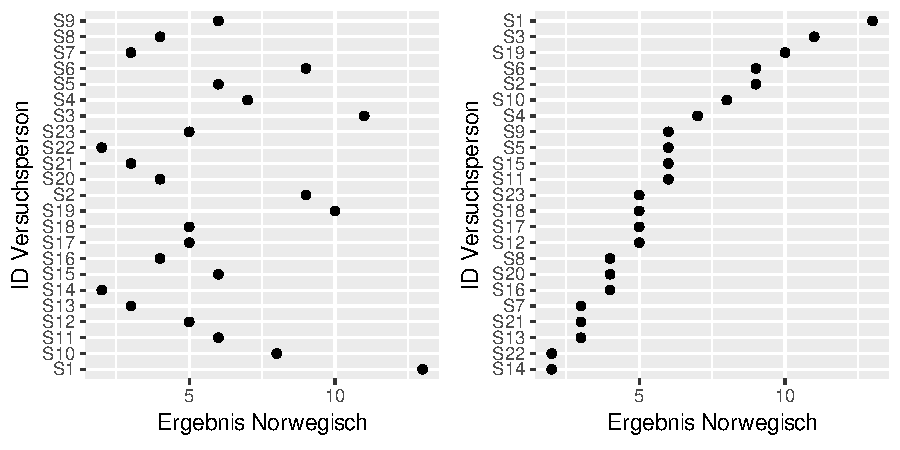
\includegraphics[width=.8\textwidth]{figs/unnamed-chunk-78-1} 

}

\caption{Ein Punktdiagramm sortiert nach den IDs der Versuchspersonen (links) und eins geordnet nach dem Ergebnis (rechts). Es gibt keine Werte, die weit von anderen liegen.\label{fig:dotchart}}\label{fig:unnamed-chunk-78}
\end{figure}

\end{knitrout}

Um die linke Grafik zu zeichnen, können Sie den unten stehenden Befehl
verwenden. Mittels des \#-Zeichens habe ich diesem Befehl mit \textbf{Kommentaren}
versehen. Diese erläutern, wie die Grafik aufgebaut ist.
Am Anfang Ihrer R-Karriere empfehle ich Ihnen, Ihren Code reichlich mit
Kommentaren auszustatten, sodass Sie ihn mehrere Wochen und Monate später
noch verstehen können. Mit der Zeit werden Sie Ihren R-Code immer besser
lesen können und dann reichen kargere Kommentare durchaus.
\begin{knitrout}
\definecolor{shadecolor}{rgb}{0.969, 0.969, 0.969}\color{fgcolor}\begin{kframe}
\begin{alltt}
\hlstd{> }\hlkwd{ggplot}\hlstd{(}\hlkwc{data} \hlstd{= d,}                \hlcom{# Datensatz mit den Variablen}
\hlstd{+ }       \hlcom{# aes() = aesthetics = welche Variable wie dargestellt werden soll}
\hlstd{+ }       \hlkwd{aes}\hlstd{(}\hlkwc{x} \hlstd{= Norwegian,}       \hlcom{# Variable auf x-Achse}
\hlstd{+ }           \hlkwc{y} \hlstd{= Participant))} \hlopt{+}  \hlcom{# Variable auf y-Achse}
\hlstd{+ }  \hlkwd{geom_point}\hlstd{()} \hlopt{+}                \hlcom{# Daten als Punkte darstellen}
\hlstd{+ }  \hlkwd{xlab}\hlstd{(}\hlstr{"Ergebnis Norwegisch"}\hlstd{)} \hlopt{+} \hlcom{# insb. bei Arbeiten/Vorträgen/Artikeln:}
\hlstd{+ }  \hlkwd{ylab}\hlstd{(}\hlstr{"ID Versuchsperson"}\hlstd{)}     \hlcom{#     Achsen beschriften}
\end{alltt}
\end{kframe}
\end{knitrout}

Achten Sie darauf, dass das \texttt{tidyverse}-Bündel
geladen ist: Auch wenn Sie es installiert haben und in einer anderen
Session verwendet haben, müssen Sie es in jeder Session erneut laden.
Achten Sie weiter auf Gross- und Kleinschreibung, auf die Klammern
und Kommas und auf die Pluszeichen. Mit Letzteren werden der Grafik
zusätzliche Schichten hinzugefügt. Mit dem
Befehl auf den ersten vier Zeilen (\texttt{ggplot(...)}) wird
lediglich die `Leinwand' der Grafik gezeichnet. Nach dem
Pluszeichen folgt der Befehl \texttt{geom\_point(...)},
der Punkte auf die Leinwand malt.
Mit den Befehlen \texttt{xlab(...)} und \texttt{ylab(...)} werden
Achsenbeschriftungen hinzugefügt bzw.\ überschrieben.
In einem \texttt{ggplot()}-Befehl werden die unterschiedlichen Schichten
mit einem +-Zeichen zusammengefügt, nicht mit einem \textit{pipe} (|>).

Um die rechte Grafik zu zeichnen, ersetzen Sie in der 4.\ Zeile
\texttt{y = Participant} durch \texttt{y = reorder(Participant, Norwegian)}
(Klammer nicht vergessen!).

\medskip

\begin{framed}
\textbf{Einschub: Code mit Stil.}
Mit dem folgenden Code können Sie ebenfalls die Grafik links
zeichnen, denn Leerzeichen und Zeilenbrüche werden von R
mehrheitlich ignoriert.
\begin{knitrout}
\definecolor{shadecolor}{rgb}{0.969, 0.969, 0.969}\color{fgcolor}\begin{kframe}
\begin{alltt}
\hlstd{> }\hlkwd{ggplot}\hlstd{(}\hlkwc{data}\hlstd{=d,}\hlkwd{aes}\hlstd{(}\hlkwc{x}\hlstd{=}
\hlstd{+ }\hlstd{Norwegian,}\hlkwc{y}\hlstd{=Participant))}\hlopt{+}\hlkwd{geom_point}\hlstd{(}
\hlstd{+ }\hlstd{)}\hlopt{+}\hlkwd{xlab}\hlstd{(}\hlstr{"Ergebnis Norwegisch"}\hlstd{)}\hlopt{+}\hlkwd{ylab}\hlstd{(}\hlstr{"ID Versuchsperson"}\hlstd{)}
\end{alltt}
\end{kframe}
\end{knitrout}
Die erste Variante ist jedoch viel übersichtlicher, denn
die Struktur des Codes (inkl.\ Einrückungen) widerspiegelt
die logische Struktur des Befehls und die Leerzeichen
machen den Code lesbarer.
Versuchen Sie daher bereits am Anfang Ihrer R-Karriere,
einen übersichtlichen und konsistenten Codierstil zu pflegen,
etwa indem Sie meinen emulieren oder sich an einer
Gestaltungsrichtlinie (z.B.\ \url{https://style.tidyverse.org/}) orientieren.
\end{framed}

\medskip

\begin{framed}
\textbf{Einschub: Grafiken speichern.}
Nachdem Sie eine Grafik mit \texttt{ggplot()}
erzeugt haben, können Sie diese mit dem Befehl
\texttt{ggsave()} speichern. Siehe hierzu \texttt{?ggsave}.

Es gibt aber eine allgemeinere Methode, die nicht nur bei von \texttt{ggplot()}
erzeugten Grafiken funktioniert. Um die linke Grafik aus Abbildung \ref{fig:dotchart}
zu speichern, können Sie den \texttt{ggplot()}-Befehlen zwischen die Befehle
\texttt{pdf()} und \texttt(dev.off()) zu stellen, wie folgt:
\begin{knitrout}
\definecolor{shadecolor}{rgb}{0.969, 0.969, 0.969}\color{fgcolor}\begin{kframe}
\begin{alltt}
\hlstd{> }\hlkwd{pdf}\hlstd{(}\hlkwd{here}\hlstd{(}\hlstr{"figs"}\hlstd{,} \hlstr{"dotchart.pdf"}\hlstd{),}
\hlstd{+ }    \hlkwc{width} \hlstd{=} \hlnum{5}\hlstd{,} \hlkwc{height} \hlstd{=} \hlnum{4}\hlstd{)} \hlcom{# Höhe und Breite in Zoll}
\hlstd{> }\hlkwd{ggplot}\hlstd{(}\hlkwc{data} \hlstd{= d,}
\hlstd{+ }       \hlkwd{aes}\hlstd{(}\hlkwc{x} \hlstd{= Norwegian,}
\hlstd{+ }           \hlkwc{y} \hlstd{= Participant))} \hlopt{+}
\hlstd{+ }  \hlkwd{geom_point}\hlstd{()} \hlopt{+}
\hlstd{+ }  \hlkwd{xlab}\hlstd{(}\hlstr{"Ergebnis Norwegisch"}\hlstd{)} \hlopt{+}
\hlstd{+ }  \hlkwd{ylab}\hlstd{(}\hlstr{"ID Versuchsperson"}\hlstd{)}
\hlstd{> }\hlkwd{dev.off}\hlstd{()}
\end{alltt}
\end{kframe}
\end{knitrout}
Die Abbildung finden Sie jetzt als eine PDF-Datei
mit dem Namen \texttt{dotchart.pdf} im Unterordner \texttt{figs} in Ihrem Projektordner.

Wenn Sie die Grafik lieber in einem anderen Format speichern, können
Sie statt \texttt{pdf()} auch \texttt{svg()}, \texttt{png()}, \texttt{tiff()} oder
\texttt{bmp()} verwenden.

Für eine schnelle Grafik können Sie natürlich auch das \texttt{Export}-Menü
in der Registerkarte \texttt{Plots} im Fenster rechts unten in RStudio verwenden.
Aber ich empfehle Ihnen, den Gebrauch von \texttt{pdf()} zu umarmen, da Sie so
in Ihrem Code dokumentieren, mit welchen Einstellungen die Grafik gespeichert wurde.
Das ist nämlich sehr praktisch, wenn Sie später alle Grafiken mit leicht anderen
Einstellungen neu zeichnen müssen.
\end{framed}

\medskip

In diesem Beispiel ist das Punktdiagramm insbesondere nützlich
aufgrund von dem, was es eben nicht aufzeigt. Es scheint
nämlich keine Datenpunkte, oder Grüppchen von Datenpunkten, zu geben,
die ziemlich weit von den anderen entfernt liegen. Solche Datenpunkte,
die man \textbf{Ausreisser} nennt, können das Ergebnis einer Analyse
stark beeinflussen, sodass es wichtig ist, zu wissen, dass es sie gibt.
Ausreisser können (nicht müssen) auch auf technische
Fehler hinweisen und sollten also nochmals kontrolliert werden.
Abbildung \ref{fig:outlier} zeigt ein fiktives Beispiel, in dem
die Anzahl morphologischer Fehler pro Textseite pro Lerner aufgeführt wird.
Ein Datenpunkt liegt so weit von den anderen entfernt, dass man hier
auf jeden Fall nochmals kontrollieren sollte, ob die Angabe tatsächlich stimmt,
und nicht etwa auf einem Tippfehler bei der Dateneingabe beruht.
\begin{knitrout}
\definecolor{shadecolor}{rgb}{0.969, 0.969, 0.969}\color{fgcolor}\begin{figure}[tp]

{\centering 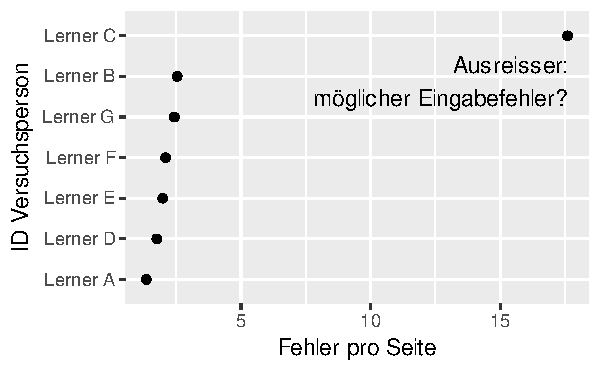
\includegraphics[width=.5\textwidth]{figs/unnamed-chunk-82-1} 

}

\caption{Beispiel eines Ausreissers. Hier müsste man kontrollieren, ob der Datenpunkt (17.6) richtig eingetragen wurde und nicht etwa ein Tippfehler ist (statt 1.76).\label{fig:outlier}}\label{fig:unnamed-chunk-82}
\end{figure}

\end{knitrout}

\section{Das Histogramm}\label{sec:histogram}
Eine zweite nützliche Grafik ist das Histogramm.
Für ein Histogramm wird die Variable, die man darstellen
möchte, in \textit{bins} aufgeteilt und es wird gezählt,
wie viele Beobachtungen es in jedem \textit{bin} gibt.
Diese Anzahlen werden in der Grafik als Bälkchen dargestellt,
siehe Abbildung \ref{fig:histogram}.
Wie in diesem Beispiel sind die \textit{bins}
in den allermeisten Histogrammen gleich breit.
Die Breite der \textit{bins} muss man selber festlegen;
wie die Befehle und Kommentare unten zeigen, ist dies
eine Frage von Ausprobieren.

Verglichen mit dem Punktdiagramm ist ein Vorteil
des Histogramms, dass auch sehr grosse Datensätze sinnvoll
dargestellt werden können, während man in einem Punktdiagramm
wohl schnell den Überblick verliert.
\begin{knitrout}
\definecolor{shadecolor}{rgb}{0.969, 0.969, 0.969}\color{fgcolor}\begin{kframe}
\begin{alltt}
\hlstd{> }\hlkwd{ggplot}\hlstd{(}\hlkwc{data} \hlstd{= d,}
\hlstd{+ }       \hlkwd{aes}\hlstd{(}\hlkwc{x} \hlstd{= Norwegian))} \hlopt{+}
\hlstd{+ }  \hlcom{# Defaulteinstellungen fürs Histogramm (immer 30 bins)}
\hlstd{+ }  \hlkwd{geom_histogram}\hlstd{()}
\hlstd{> }
\hlstd{> }\hlkwd{ggplot}\hlstd{(}\hlkwc{data} \hlstd{= d,}
\hlstd{+ }       \hlkwd{aes}\hlstd{(}\hlkwc{x} \hlstd{= Norwegian))} \hlopt{+}
\hlstd{+ }  \hlcom{# Anzahl 'bins' definieren}
\hlstd{+ }  \hlkwd{geom_histogram}\hlstd{(}\hlkwc{bins} \hlstd{=} \hlnum{10}\hlstd{)}
\hlstd{> }
\hlstd{> }\hlkwd{ggplot}\hlstd{(}\hlkwc{data} \hlstd{= d,}
\hlstd{+ }       \hlkwd{aes}\hlstd{(}\hlkwc{x} \hlstd{= Norwegian))} \hlopt{+}
\hlstd{+ }  \hlcom{# Binbreite definieren}
\hlstd{+ }  \hlkwd{geom_histogram}\hlstd{(}\hlkwc{binwidth} \hlstd{=} \hlnum{3}\hlstd{)}
\hlstd{> }
\hlstd{> }\hlkwd{ggplot}\hlstd{(}\hlkwc{data} \hlstd{= d,}
\hlstd{+ }       \hlkwd{aes}\hlstd{(}\hlkwc{x} \hlstd{= Norwegian))} \hlopt{+}
\hlstd{+ }  \hlcom{# Grenzen selbst festlegen, hier etwa bei 0, 4, 8, 12, 16.}
\hlstd{+ }  \hlcom{# Kürzel: seq(from = 0, to = 16, by = 4).}
\hlstd{+ }  \hlcom{# Die Farben kann man selbst auswählen.}
\hlstd{+ }  \hlkwd{geom_histogram}\hlstd{(}\hlkwc{breaks} \hlstd{=} \hlkwd{seq}\hlstd{(}\hlkwc{from} \hlstd{=} \hlnum{0}\hlstd{,} \hlkwc{to} \hlstd{=} \hlnum{16}\hlstd{,} \hlkwc{by} \hlstd{=} \hlnum{4}\hlstd{),}
\hlstd{+ }                 \hlkwc{fill} \hlstd{=} \hlstr{"lightgreen"}\hlstd{,}
\hlstd{+ }                 \hlkwc{colour} \hlstd{=} \hlstr{"darkgreen"}\hlstd{)} \hlopt{+}
\hlstd{+ }  \hlcom{# Achsenbezeichnungen}
\hlstd{+ }  \hlkwd{xlab}\hlstd{(}\hlstr{"Ergebnisse cloze-Test Norwegisch"}\hlstd{)} \hlopt{+}
\hlstd{+ }  \hlkwd{ylab}\hlstd{(}\hlstr{"Anzahl Studierende"}\hlstd{)}
\end{alltt}
\end{kframe}
\end{knitrout}


\begin{knitrout}
\definecolor{shadecolor}{rgb}{0.969, 0.969, 0.969}\color{fgcolor}\begin{figure}[tp]

{\centering 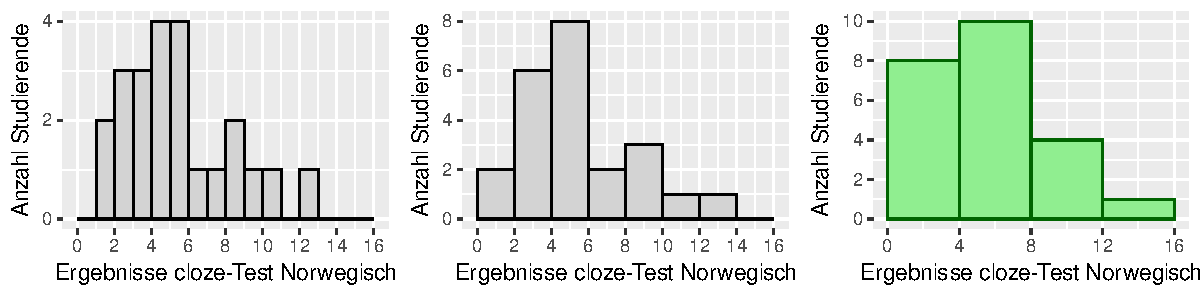
\includegraphics[width=\textwidth]{figs/unnamed-chunk-84-1} 

}

\caption{Drei Histogramme mit den \texttt{Norwegian}-Ergebnissen. \textit{Links}: Die Grenzen zwischen den \textit{bins} liegen bei 0, 1, 2, usw., 15, 16. \textit{Mitte}: Grenzen bei 0, 2, 4, usw., 15, 16. \textit{Rechts}: Grenzen bei 0, 4, 8, 12, 16. Sowohl die Grafik links als auch die in der Mitte halte ich hier für sinnvoll; die Grafik rechts ist nach meinem Geschmack ein bisschen zu grob. Eine goldene Regel für die Wahl der Breite der \textit{bins} gibt es nicht. Daher gilt: Mit den Einstellungen herumspielen und eine nützliche Grafik auswählen.\label{fig:histogram}}\label{fig:unnamed-chunk-84}
\end{figure}

\end{knitrout}
 
In den Histogrammen bisher stand die Anzahl
Beobachtungen pro \textit{bin} auf der $y$-Achse.
Wenn man unterschiedliche Histogramme (z.B.\ von unterschiedlichen
Gruppen) vergleichen möchte, kann es sinnvoller sein, diese
Zahlen zu einer Art relative Frequenz umzurechnen.
Diese nennt man \textbf{Wahrscheinlichkeitsdichten}.
Sie werden so berechnet, dass die Gesamtfläche, die das Histogramm
einnimmt, 1 beträgt. Anders gesagt: Man nimmt die Höhe jedes \textit{bins},
also die Wahrscheinlichkeitsdichte, und multipliziert diese mit seiner Breite,
um die Oberfläche der Bälkchen zu berechnen. Die Höhe wird so festgelegt,
dass wenn man alle Oberflächen addiert, die Summe 1 beträgt. Die Form
des Histogramms ist aber gleich, egal ob man mit den Anzahlen oder den
Wahrscheinlichkeitsdichten arbeitet.

Abbildung \ref{fig:histogramdensity} zeigt ein Beispiel.
Die Breite jedes \textit{bins} in der rechten Grafik beträgt 4.
Die Höhen sind etwa 0.09, etwa 0.105, etwa 0.045 und fast 0.015, sodass
$(4 \cdot 0.09) + (4 \cdot 0.105) + (4 \cdot 0.045) + (4 \cdot 0.015) \approx 1$.
\begin{knitrout}
\definecolor{shadecolor}{rgb}{0.969, 0.969, 0.969}\color{fgcolor}\begin{figure}[tp]

{\centering 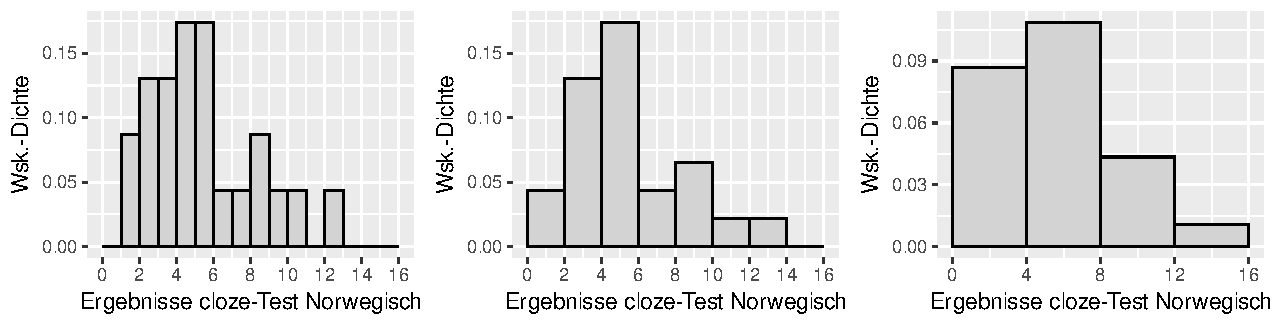
\includegraphics[width=\textwidth]{figs/unnamed-chunk-85-1} 

}

\caption{Drei Histogramme mit der \texttt{Norwegian}-Ergebnissen. Statt der absoluten Anzahl Beobachtungen pro \textit{bin} stehen hier Wahrscheinlichkeitsdichten auf der y-Achse.\label{fig:histogramdensity}}\label{fig:unnamed-chunk-85}
\end{figure}

\end{knitrout}

Um die Grafiken in Abbildung \ref{fig:histogramdensity} selber zu zeichnen, ersetzen
Sie in den Befehlen oben
\begin{knitrout}
\definecolor{shadecolor}{rgb}{0.969, 0.969, 0.969}\color{fgcolor}\begin{kframe}
\begin{alltt}
\hlstd{> }\hlkwd{ggplot}\hlstd{(}\hlkwc{data} \hlstd{= d,}
\hlstd{+ }       \hlkwd{aes}\hlstd{(}\hlkwc{x} \hlstd{= Norwegian))}
\end{alltt}
\end{kframe}
\end{knitrout}
durch
\begin{knitrout}
\definecolor{shadecolor}{rgb}{0.969, 0.969, 0.969}\color{fgcolor}\begin{kframe}
\begin{alltt}
\hlstd{> }\hlkwd{ggplot}\hlstd{(}\hlkwc{data} \hlstd{= d,}
\hlstd{+ }       \hlkwd{aes}\hlstd{(}\hlkwc{x} \hlstd{= Norwegian,}
\hlstd{+ }           \hlkwc{y} \hlstd{= ..density..))}
\end{alltt}
\end{kframe}
\end{knitrout}


\section{Mittelwerte}
Es ist unpraktisch, in einem Bericht alle einzelnen
beobachteten Werte aufzulisten.\footnote{Aber es ist sehr sinnvoll,
den Datensatz online verfügbar zu stellen und im Bericht auf ihn
zu verweisen; siehe \citet{Klein2018} und \citet{Levenstein2018}! Eine benutzerfreundliche Website, wo Sie dies machen können, ist \url{https://osf.io}; siehe \citet{Soderberg2018} für eine Anleitung.} Wenn möglich probiert
man diese Informationen daher zu komprimieren, indem
man berichtet, welcher Wert typisch für diese Beobachtungen
ist und wie sehr die einzelnen Beobachtungen von diesem
typischen Wert abweichen.
Die Frage nach dem typischen Wert betrifft die \textbf{zentrale Tendenz}
der Beobachtungen und wird anhand von einem Mittelwert
beantwortet. Die Frage nach den Abweichungen betrifft die
\textbf{Streuung} der Beobachtungen und wird anhand von Streuungsmassen
beantwortet. Zuerst widmen wir uns den Mittelwerten.

\subsection{Das arithmetische Mittel}
Wenn man vom `Durchschnitt' oder `Mittelwert' spricht,
meint man meistens das (arithmetische) Mittel.
Eigentlich sind `Durchschnitt' und `Mittelwert' aber Hyperonyme,
denn es gibt ausser dem Mittel noch andere Durchschnittsmasse.

Um das Mittel zu berechnen, addiert
man alle Werte und teilt man die Summe durch die Anzahl Werte.
Das Populationsmittel kürzt man in Formeln meistens als $\mu$ ab.
In Gross-Sigmanotation schaut die Formel so aus:\footnote{Ich
erlaube mir hier etwas mathematische Unvollständigkeit zwecks
didaktischer Deutlichkeit. Die Formel gilt nämlich nur
für Populationen, die nur endlich viele Elemente enthalten.
Die Formel für unendlich grosse Populationen erspare ich hier Ihnen,
da Sie erstens wesentlich schwieriger und zweitens nicht so wichtig ist.}
\begin{equation*}
\mu = \frac{1}{N} \sum_{i = 1}^{N} x_i.
\end{equation*}

\medskip

\begin{framed}\label{grosssigma}
\textbf{Einschub: Gross-Sigmanotation.} Formeln wie diese mögen abschrecken,
sind in Statistikhandbüchern jedoch gang und gäbe---und gar nicht so schwierig.

Reihen von Beobachtungen einer Variablen (`Vektoren') werden meistens mit
römischen Buchstaben dargestellt. `$x$' ist also die Reihe von Beobachtungen,
deren Mittel wir berechnen wollen---hier also die 23 Ergebnisse beim norwegischen
Lesetest.

Das kleine `$i$' ist ein Index und wird verwendet um eine spezifische Beobachtung
zu identifizieren. `$x_i$' heisst lediglich `die i.\ Beobachtung von $x$'. Ist $i$ gleich 5,
dann heisst $x_i$ eigentlich $x_5$, sprich die 5.\ Beobachtung von $x$.

`$N$' ist einfach die Anzahl Beobachtungen in der Reihe---bei uns also $N = 23$.

`$\sum$', zu guter Letzt, heisst lediglich `Summe'. Die Werte, die wir
addieren müssen, kommen nach dem Symbol. $\sum_{i = 1}^{N} x_i$ heisst,
dass wir die Werte in der Reihe $x$ addieren müssen, anfangend mit dem ersten ($i = 1$)
und endend beim letzten ($N$).
$\sum_{i = 3}^{5} x_i$ hiesse, dass
wir nur den 3., 4.\ und 5.\ $x$-Wert addieren müssten.

Der Ausdruck
\[
  \frac{1}{N} \sum_{i = 1}^{N} x_i
\]
kann also so umgeschrieben werden:
\[
  \frac{1}{N}(x_1 + x_2 + x_3 + \dots + x_N).
\]

In unserem Beispiel:
\[
  \frac{1}{23}(13 + 9 + 11 + \dots + 5).
\]
\end{framed}

\medskip

\begin{framed}
\textbf{Einschub: \textit{for}-Schleifen.}
Der Einschub zur Gross-Sigmanotation gibt uns die Gelegenheit,
\textit{for}-Schleifen vorzustellen. Mit einer \textit{for}-Schleife
kann man Berechnungen iterativ ausführen. Der folgende Codeabschnitt
etwa kreiert zunächst eine Variable namens
\texttt{resultat} und initalisiert diese mit 0.
Dann wird eine \textit{for}-Schleife geöffnet, in welcher der
Index \texttt{i} die Ganzzahlen von 1 bis und mit 10 durchläuft.
Bei jedem Durchgang der \textit{for}-Schleife wird
der Index \texttt{i} zum jetzigen Wert von \texttt{resultat}
addiert; die Summe gilt als neuer Wert von \texttt{resultat}.
Danach, bei der schliessenden geschweiften Klammer, wird der
nächste Index verwendet. Wenn alle Indizes durchlaufen wurden,
hört die \textit{for}-Schleife auf.
Dieser Codeabschnitt berechnet also lediglich die Summe
der Ganzzahlen 1 bis und mit 10 (in Gross-Sigmanotation: $\sum_{i=1}^{10} i$):
\begin{knitrout}
\definecolor{shadecolor}{rgb}{0.969, 0.969, 0.969}\color{fgcolor}\begin{kframe}
\begin{alltt}
\hlstd{> }\hlstd{resultat} \hlkwb{<-} \hlnum{0}
\hlstd{> }\hlkwa{for} \hlstd{(i} \hlkwa{in} \hlnum{1}\hlopt{:}\hlnum{10}\hlstd{) \{}
\hlstd{+ }  \hlstd{resultat} \hlkwb{<-} \hlstd{resultat} \hlopt{+} \hlstd{i}
\hlstd{+ }\hlstd{\}}
\hlstd{> }\hlstd{resultat}
\end{alltt}
\begin{verbatim}
[1] 55
\end{verbatim}
\end{kframe}
\end{knitrout}

Für diese Berechnung steht uns in R natürlich auch eine spezialisierte
(und schnellere) Funktion zur Verfügung:
\begin{knitrout}
\definecolor{shadecolor}{rgb}{0.969, 0.969, 0.969}\color{fgcolor}\begin{kframe}
\begin{alltt}
\hlstd{> }\hlkwd{sum}\hlstd{(}\hlnum{1}\hlopt{:}\hlnum{10}\hlstd{)}
\end{alltt}
\begin{verbatim}
[1] 55
\end{verbatim}
\end{kframe}
\end{knitrout}

Wir können den Index auch verwenden, um auf Elemente in Vektoren oder Listen zuzugreifen.
Eine umständliche Art und Weise, um die Summe der Norwegischwerte zu berechnen,
ist daher die folgende:
\begin{knitrout}
\definecolor{shadecolor}{rgb}{0.969, 0.969, 0.969}\color{fgcolor}\begin{kframe}
\begin{alltt}
\hlstd{> }\hlstd{resultat} \hlkwb{<-} \hlnum{0}
\hlstd{> }\hlkwa{for} \hlstd{(i} \hlkwa{in} \hlnum{1}\hlopt{:}\hlkwd{length}\hlstd{(d}\hlopt{$}\hlstd{Norwegian)) \{}
\hlstd{+ }  \hlstd{resultat} \hlkwb{<-} \hlstd{resultat} \hlopt{+} \hlstd{d}\hlopt{$}\hlstd{Norwegian[[i]]}
\hlstd{+ }\hlstd{\}}
\hlstd{> }\hlstd{resultat}
\end{alltt}
\begin{verbatim}
[1] 136
\end{verbatim}
\begin{alltt}
\hlstd{> }\hlcom{# besser:}
\hlstd{> }\hlcom{# sum(d$Norwegian)}
\end{alltt}
\end{kframe}
\end{knitrout}

Die Notation \texttt{d\$Norwegian} zieht den Vektor namens \texttt{Norwegian} aus dem tibble \texttt{d}.
Mit der Funktion \texttt{length()} fragt man die Anzahl Elemente, die dieser Vektor enthält,
ab.
Da der Vektor 23 Werte zählt, heisst \texttt{1:length(d\$Norwegian)} so viel wie \texttt{1:23}.
In der \texttt{for}-Schleife wird nun statt des Indexes \texttt{i} jeweils der $i.$ Werte zum
bisherigen Resultat addiert.
Die Notation \texttt{d\$Norwegian[[4]]} identifiziert den 4.\ Wert eines Vektors oder einer Liste. Statt der Notation `[[' werden Sie auch oft `[' antreffen. Der Unterschied ist hier nicht so wichtig, aber mit `[[' identifiziert man immer einen Wert; mit `[' kann man auch mehrere Werte gleichzeitig abfragen.

Wenn wir nicht nur das Endergebnis haben möchten, sondern auch die Zwischenergebnisse,
können wir wie folgt vorgehen.
Zunächst kreieren wir einen Vektor mit Platz für 10 Werte; hier werden wir die
Zwischenresultate abspeichern. Das erste Zwischenergebnis, 1, stellen wir manuell
ein. In der \textit{for}-Schleife durchläuft der Index alle Werte von 2 (!) bis 10.
Im $i.$ Durchgang wird der aktuelle Index zum letzten Zwischenergebnis addiert;
die Summe wird dann in den Vektor in die $i.$ Stelle des Vektors abgelagert:
\begin{knitrout}
\definecolor{shadecolor}{rgb}{0.969, 0.969, 0.969}\color{fgcolor}\begin{kframe}
\begin{alltt}
\hlstd{> }\hlstd{zwresultate} \hlkwb{<-} \hlkwd{vector}\hlstd{(}\hlkwc{length} \hlstd{=} \hlnum{10}\hlstd{)}
\hlstd{> }\hlstd{zwresultate[[}\hlnum{1}\hlstd{]]} \hlkwb{<-} \hlnum{1}
\hlstd{> }\hlkwa{for} \hlstd{(i} \hlkwa{in} \hlnum{2}\hlopt{:}\hlnum{10}\hlstd{) \{}
\hlstd{+ }  \hlstd{zwresultate[[i]]} \hlkwb{<-} \hlstd{zwresultate[[i}\hlopt{-}\hlnum{1}\hlstd{]]} \hlopt{+} \hlstd{i}
\hlstd{+ }\hlstd{\}}
\hlstd{> }\hlstd{zwresultate}
\end{alltt}
\begin{verbatim}
 [1]  1  3  6 10 15 21 28 36 45 55
\end{verbatim}
\end{kframe}
\end{knitrout}

Schneller mit \texttt{cumsum()} (\textit{cumulative sum}):
\begin{knitrout}
\definecolor{shadecolor}{rgb}{0.969, 0.969, 0.969}\color{fgcolor}\begin{kframe}
\begin{alltt}
\hlstd{> }\hlkwd{cumsum}\hlstd{(}\hlnum{1}\hlopt{:}\hlnum{10}\hlstd{)}
\end{alltt}
\begin{verbatim}
 [1]  1  3  6 10 15 21 28 36 45 55
\end{verbatim}
\end{kframe}
\end{knitrout}

Wir müssen in der \textit{for}-Schleife bei 2 statt bei 1 anfangen,
da \texttt{zwresultate} keinen $1-1 = 0.$\ Wert hat.
\begin{knitrout}
\definecolor{shadecolor}{rgb}{0.969, 0.969, 0.969}\color{fgcolor}\begin{kframe}
\begin{alltt}
\hlstd{> }\hlstd{zwresultate} \hlkwb{<-} \hlkwd{vector}\hlstd{(}\hlkwc{length} \hlstd{=} \hlnum{10}\hlstd{)}
\hlstd{> }\hlstd{zwresultate[[}\hlnum{1}\hlstd{]]} \hlkwb{<-} \hlnum{1}
\hlstd{> }\hlkwa{for} \hlstd{(i} \hlkwa{in} \hlnum{1}\hlopt{:}\hlnum{10}\hlstd{) \{}
\hlstd{+ }  \hlstd{zwresultate[[i]]} \hlkwb{<-} \hlstd{zwresultate[[i}\hlopt{-}\hlnum{1}\hlstd{]]} \hlopt{+} \hlstd{i}
\hlstd{+ }\hlstd{\}}
\end{alltt}


{\ttfamily\noindent\bfseries\color{errorcolor}{Error in zwresultate[[i - 1]]: attempt to select less than one element in get1index <real>}}\end{kframe}
\end{knitrout}

Wer sich ein bisschen mit Programmiersprachen auskennt, hat
aus diesen Beispielen auch gelernt, dass das erste Element
eines Vektors in R den Index 1 hat. Programmiersprachen
wie Java und Python verweisen auf das erste Element mit dem Index 0.
\end{framed}

Das Mittel der Norwegischdaten können wir folgendermassen
berechnen:
\begin{knitrout}
\definecolor{shadecolor}{rgb}{0.969, 0.969, 0.969}\color{fgcolor}\begin{kframe}
\begin{alltt}
\hlstd{> }\hlcom{# Summe aller Norwegian-Werte}
\hlstd{> }\hlkwd{sum}\hlstd{(d}\hlopt{$}\hlstd{Norwegian)}
\end{alltt}
\begin{verbatim}
[1] 136
\end{verbatim}
\begin{alltt}
\hlstd{> }\hlcom{# Anzahl Norwegian-Werte}
\hlstd{> }\hlkwd{length}\hlstd{(d}\hlopt{$}\hlstd{Norwegian)}
\end{alltt}
\begin{verbatim}
[1] 23
\end{verbatim}
\begin{alltt}
\hlstd{> }\hlcom{# Summe geteilt durch Anzahl}
\hlstd{> }\hlnum{136}\hlopt{/}\hlnum{23}
\end{alltt}
\begin{verbatim}
[1] 5.913
\end{verbatim}
\begin{alltt}
\hlstd{> }\hlcom{# Oder in einer Zeile}
\hlstd{> }\hlkwd{sum}\hlstd{(d}\hlopt{$}\hlstd{Norwegian)} \hlopt{/} \hlkwd{length}\hlstd{(d}\hlopt{$}\hlstd{Norwegian)}
\end{alltt}
\begin{verbatim}
[1] 5.913
\end{verbatim}
\end{kframe}
\end{knitrout}

Einfacher geht es mit der \texttt{mean()}-Funktion:
\begin{knitrout}
\definecolor{shadecolor}{rgb}{0.969, 0.969, 0.969}\color{fgcolor}\begin{kframe}
\begin{alltt}
\hlstd{> }\hlkwd{mean}\hlstd{(d}\hlopt{$}\hlstd{Norwegian)}
\end{alltt}
\end{kframe}
\end{knitrout}
Anders als im letzten Kapitel brauchen wir die zusätzliche Einstellung
\texttt{na.rm = TRUE} hier nicht, da die Variable keine fehlenden Daten
enthält.

Die \texttt{tidyverse}-Lösung brauchen wir hier im Prinzip
nicht, aber sie zeigt nochmals, wie die \texttt{summarise()}-Funktion
funktioniert.
\begin{knitrout}
\definecolor{shadecolor}{rgb}{0.969, 0.969, 0.969}\color{fgcolor}\begin{kframe}
\begin{alltt}
\hlstd{> }\hlstd{d |>}
\hlstd{+ }  \hlkwd{summarise}\hlstd{(}\hlkwc{mittel_norwegisch} \hlstd{=} \hlkwd{mean}\hlstd{(Norwegian))}
\end{alltt}
\begin{verbatim}
# A tibble: 1 x 1
  mittel_norwegisch
              <dbl>
1              5.91
\end{verbatim}
\end{kframe}
\end{knitrout}

Das Mittel hat ein paar nützliche mathematische Eigenschaften,
denen es seine Omnipräsenz verdankt. Eine betrifft den zentralen Grenzwertsatz; siehe Abschnitt \ref{sec:clt}.
Ein wesentlicher Nachteil des Mittels ist aber, dass er stark von Ausreissern beeinflusst wird.
Nimmt man zum Beispiel die Daten aus Abbildung \vref{fig:outlier} und berechnet man ihr Mittel,
dann ist das Ergebnis 4.25---ein ziemlich untypischer Wert für die Beobachtungen,
sind doch 6 der 7 Beobachtungen unter 2.6 und 1 über 17.5. Lässt man den Ausreisser weg,
ist das Mittel 2.02, was der Tendenz des Hauptanteils der Beobachtungen besser entspricht.

\subsection{Der Median}
Ein anderer beliebter Mittelwert ist der Median.
Es handelt sich hier buchstäblich um den Wert in der Mitte:
Zum Berechnen des Medians ordnet man die Daten
von klein nach gross und nimmt man den mittleren Wert.
Gibt es eine gerade Anzahl Beobachtungen, gibt es zwei
mittlere Werte. In solchen Fällen ist der Median das Mittel beider
mittlerer Werte.

Zuerst die komplizierte Berechnungsmethode,
um den Vorgang zu illustrieren: Mit \texttt{arrange()}
die Daten von klein nach gross ordnen und dann den mittleren Wert
nehmen. Da es 23 Beobachtungen gibt,
ist der 12.\ Wert der mittlere
(es gibt 11 kleinere und 11 grössere):
\begin{knitrout}
\definecolor{shadecolor}{rgb}{0.969, 0.969, 0.969}\color{fgcolor}\begin{kframe}
\begin{alltt}
\hlstd{> }\hlstd{d |>}
\hlstd{+ }  \hlkwd{select}\hlstd{(Norwegian) |>}
\hlstd{+ }  \hlkwd{arrange}\hlstd{(Norwegian) |>}
\hlstd{+ }  \hlkwd{slice}\hlstd{(}\hlnum{12}\hlstd{)}
\end{alltt}
\begin{verbatim}
# A tibble: 1 x 1
  Norwegian
      <dbl>
1         5
\end{verbatim}
\end{kframe}
\end{knitrout}

Oder kürzer mit \texttt{median()}:
\begin{knitrout}
\definecolor{shadecolor}{rgb}{0.969, 0.969, 0.969}\color{fgcolor}\begin{kframe}
\begin{alltt}
\hlstd{> }\hlkwd{median}\hlstd{(d}\hlopt{$}\hlstd{Norwegian)}
\end{alltt}
\begin{verbatim}
[1] 5
\end{verbatim}
\end{kframe}
\end{knitrout}

Mit der \texttt{summarise()}-Funktion können wir eine Zusammenfassungstabelle mit mehreren Werten aufstellen:
\begin{knitrout}
\definecolor{shadecolor}{rgb}{0.969, 0.969, 0.969}\color{fgcolor}\begin{kframe}
\begin{alltt}
\hlstd{> }\hlstd{d |>}
\hlstd{+ }  \hlkwd{summarise}\hlstd{(}\hlkwc{mittel_norwegisch} \hlstd{=} \hlkwd{mean}\hlstd{(Norwegian),}
\hlstd{+ }            \hlkwc{median_norwegisch} \hlstd{=} \hlkwd{median}\hlstd{(Norwegian))}
\end{alltt}
\begin{verbatim}
# A tibble: 1 x 2
  mittel_norwegisch median_norwegisch
              <dbl>             <dbl>
1              5.91                 5
\end{verbatim}
\end{kframe}
\end{knitrout}

Der Median ist weniger ausreisserempfindlich als das Mittel. Berechnet
man für die Werte aus Abbildung \ref{fig:outlier} den Median mit
dem Ausreisser, ist das Ergebnis 2.09; ohne ist es 2.04.

Grosse Unterschiede zwischen dem Mittel und
dem Median sind öfters
Ausreissern oder asymmetrischen Verteilungen (siehe Abschnitt
\ref{sec:distributions}) zuzuschreiben.
So oder so gilt: \textbf{Keine Mittelwerte berechnen,
ohne die Daten zuerst
grafisch darzustellen!}
Die Berechnung mag stimmen, aber unter Umständen ist sie nicht
\emph{sinnvoll}.

\subsection{Der Modus}
Den Modus trifft man weniger oft an, aber er ist eine ganz einfache
Art und Weise, um den `typischen Wert' zu definieren: Es handelt
sich schlicht und einfach um den Wert, der am häufigsten vorkommt.
Eine Modusfunktion gibt es nicht, aber wir können mit \texttt{count()} für jeden Wert
zählen, wie oft er vorkommt. Mit \texttt{arrange(desc(n))} sortieren
wir diese Anzahlen in absteigender Reihenfolge:
\begin{knitrout}
\definecolor{shadecolor}{rgb}{0.969, 0.969, 0.969}\color{fgcolor}\begin{kframe}
\begin{alltt}
\hlstd{> }\hlstd{d |>}
\hlstd{+ }  \hlkwd{count}\hlstd{(Norwegian) |>}
\hlstd{+ }  \hlkwd{arrange}\hlstd{(}\hlkwd{desc}\hlstd{(n))}
\end{alltt}
\begin{verbatim}
# A tibble: 11 x 2
  Norwegian     n
      <dbl> <int>
1         5     4
2         6     4
3         3     3
4         4     3
5         2     2
6         9     2
7         7     1
# ... with 4 more rows
\end{verbatim}
\end{kframe}
\end{knitrout}
Zwei Werte kommen am häufigsten vor: 5 und 6 kommen beide 4 Mal vor. Die Modi der Norwegischdaten sind also 5 und 6.

Ein wesentlicher Nachteil des Modus ist, dass bei feinkörnigen
Daten jede Beobachtung
eh nur ein oder zwei Mal vorkommt, sodass es nicht sinnvoll ist,
ihn zu berechnen.

\subsection{Andere Mittelwerte}
Es existieren noch weitere Mittelwerte,
z.B.\ das \textbf{harmonische Mittel},
das \textbf{geometrische Mittel},
das \textbf{winsorisierte Mittel}
und das \textbf{gewichtete Mittel}.
Diese seien hier nur der Vollständigkeit halber erwähnt,
werden aber nicht weiter erläutert.
Das \textbf{getrimmte Mittel} wird jedoch kurz vorgestellt,
da es in einer Aufgabe in einem späteren Kapitel zur Sprache
kommt.

Um ein getrimmtes Mittel zu berechnen,
löscht man zunächst die $x\%$ kleinsten und die $x\%$ grössten Werte.
Danach berechnet man das Mittel der übrig gebliebenen Werte.
Fürs 25\% getrimmte Mittel
löscht man also zwei Mal ein Viertel der Daten: die 25\% niedrigsten
Beobachtungen und die 25\% höchsten Beobachtungen.
Das getrimmte Mittel wird verwendet, um den Einfluss von extremen
Beobachtungen auf das Ergebnis zu reduzieren.
\begin{knitrout}
\definecolor{shadecolor}{rgb}{0.969, 0.969, 0.969}\color{fgcolor}\begin{kframe}
\begin{alltt}
\hlstd{> }\hlcom{# Norwegischdaten sortiert von klein nach gross}
\hlstd{> }\hlstd{norwegisch_sortiert} \hlkwb{<-} \hlkwd{sort}\hlstd{(d}\hlopt{$}\hlstd{Norwegian)}
\hlstd{> }\hlstd{norwegisch_sortiert}
\end{alltt}
\begin{verbatim}
 [1]  2  2  3  3  3  4  4  4  5  5  5  5  6  6  6  6  7  8
[19]  9  9 10 11 13
\end{verbatim}
\begin{alltt}
\hlstd{> }\hlcom{# 25% getrimmte Mittel:}
\hlstd{> }\hlkwd{mean}\hlstd{(norwegisch_sortiert,} \hlkwc{trim} \hlstd{=} \hlnum{0.25}\hlstd{)}
\end{alltt}
\begin{verbatim}
[1] 5.4615
\end{verbatim}
\begin{alltt}
\hlstd{> }\hlcom{# 1/4 von 23 ist 5.75; diese Zahl wird nach unten abgerundet, }
\hlstd{> }\hlcom{# also werden die 5 niedrigsten und 5 höchsten Werte gelöscht:}
\hlstd{> }\hlkwd{mean}\hlstd{(norwegisch_sortiert[}\hlnum{6}\hlopt{:}\hlnum{18}\hlstd{])}
\end{alltt}
\begin{verbatim}
[1] 5.4615
\end{verbatim}
\end{kframe}
\end{knitrout}

% \paragraph{Das harmonische Mittel.}



% \paragraph{Das winsorisierte Mittel.}
% Die $x\%$ kleinsten und die $x\%$ grössten Werte werden ersetzt und
% zwar durch den kleinsten bzw.\ grössten Wert, der nicht ersetzt wurde.
% Danach berechnet man das Mittel. Wenn man zum Beispiel 100 Beobachtungen
% hat und auf jeder Seite 10\% der Beobachtungen winsorisiert, ersetzt
% man die 10 niedrigsten Beobachtungen alle durch den 11.\ niedrigsten Wert
% und die 10 höchsten Beobachtungen durch den 90.\ Wert.
% In diesem Beispiel wird durch die Winsorisierung eine Ganzzahl der Datenmenge ersetzt (also 10 Beobachtungen auf jeder Seite). Die genaue Berechnung ist schwieriger, wenn durch die Winsorisierung eigentlich eine Bruchzahl der Beobachtungen ersetzt werden soll. Zum Beispiel müsste man bei einer Datenreihe von 23 Beobachtungen 2.3 Beobachtungen winsorisieren, wenn man 10\%-Winsorisierung durchführt. In solchen Fällen wird nicht der kleinste bzw.\ höchste nicht-ausgeschlossene Wert verwendet, sondern eine Intrapolation zwischen den ausgeschlossenen und den nicht-ausgeschlossenen Werten. Siehe die Funktion \texttt{winsor.mean()} im \texttt{psych}-Paket.
% Das winsorisierte Mittel wird ebenfalls verwendet, um den Einfluss
% von extremen Beobachtungen auf das Ergebnis
% zu reduzieren.

% Es gibt noch andere Mittelwerte---etwa das
% geometrische und das harmonische Mittel.
% Diese werden hier nicht behandelt.
% Auch das gewichtete Mittel wird hier nicht behandelt.

\section{Streuungsmasse}
Wenn man nur einen oder ein paar Mittelwerte berichtet,
bleibt die Frage unbeantwortet, wie stark die einzelnen
Beobachtungen davon abweichen.
Mit Streuungmassen versucht man diese Abweichnung numerisch
auszudrücken.

\subsection{Spannweite}
Ein einfaches Streuungsmass ist die Spannweite. Man berechnet
lediglich den niedrigsten und den höchsten Wert und berichtet diese oder
den Unterschied zwischen ihnen:
\begin{knitrout}
\definecolor{shadecolor}{rgb}{0.969, 0.969, 0.969}\color{fgcolor}\begin{kframe}
\begin{alltt}
\hlstd{> }\hlkwd{min}\hlstd{(d}\hlopt{$}\hlstd{Norwegian)}
\end{alltt}
\begin{verbatim}
[1] 2
\end{verbatim}
\begin{alltt}
\hlstd{> }\hlkwd{max}\hlstd{(d}\hlopt{$}\hlstd{Norwegian)}
\end{alltt}
\begin{verbatim}
[1] 13
\end{verbatim}
\begin{alltt}
\hlstd{> }\hlkwd{range}\hlstd{(d}\hlopt{$}\hlstd{Norwegian)}
\end{alltt}
\begin{verbatim}
[1]  2 13
\end{verbatim}
\end{kframe}
\end{knitrout}

Dieses Mass wird aus gutem Grund selten verwendet:
Es ist extrem ausreisserempfindlich.
Ausserdem unterschätzt die Spannweite einer
Stichprobe systematisch die Spannweite der Population,
aus der sie stammt.\footnote{Diese Tatsache scheint
übrigens in der Zweit\-sprachs\-erwerbs\-forschung
nicht allen Forschenden bekannt zu sein,
die diesem Streuuungsmass eine zentrale Rolle in ihrer Forschung zuteilen
\citep{Vanhove2019b}.}
(Mit Stichproben beschäftigen
wir uns in späteren Kapiteln.)

\subsection{Summe der Quadrate}\label{sec:sumsofsquares}
Wenn wir alle Beobachtungen ins Streuungsmass einfliessen lassen wollen,
scheint es auf den ersten Blick sinnvoll, die Unterschiede zwischen den beobachteten
Werten und dem Mittel zu berechnen und diese Unterschiede beieinander aufzuzählen:
$(x_1 - \mu) + (x_2 - \mu) + \dots$. Diese Summe ist aber immer 0.
Um das zu sehen, überlege man sich Folgendes:
\[
  (x_1 - \mu) + (x_2 - \mu) + \dots + (x_N - \mu) = (x_1 + x_2 + \dots + x_N) - N\mu.
\]
Nun wird $\mu$ berechnet als $\frac{1}{N}(x_1 + x_2 + \dots + x_N)$,
sodass $N\mu = x_1 + x_2 + \dots + x_N$. Daher gilt
\[
  (x_1 + x_2 + \dots + x_N) - N\mu = (x_1 + x_2 + \dots + x_N) - (x_1 + x_2 + \dots + x_N) = 0.
\]
Um dieses Problem zu lösen, werden die Unterschiede zwischen den beobachteten
Werten und dem Mittel quadriert, bevor sie beieinander aufgezählt werden.
Dadurch werden sie alle positiv, sodass ihre Summe nicht länger 0 ist.
Diese Summe der Quadrate wird in Formeln als $d^2$ oder $SS$ (\textit{sum of squares}) abgekürzt:
\begin{equation*}
d^2 = \sum_{i = 1}^{N} (x_i - \mu)^2.
\end{equation*}
\begin{knitrout}
\definecolor{shadecolor}{rgb}{0.969, 0.969, 0.969}\color{fgcolor}\begin{kframe}
\begin{alltt}
\hlstd{> }\hlkwd{sum}\hlstd{((d}\hlopt{$}\hlstd{Norwegian} \hlopt{-} \hlkwd{mean}\hlstd{(d}\hlopt{$}\hlstd{Norwegian))}\hlopt{^}\hlnum{2}\hlstd{)}
\end{alltt}
\begin{verbatim}
[1] 187.83
\end{verbatim}
\end{kframe}
\end{knitrout}
Achten Sie auf die Stelle der Klammern und der Quadrierung: Die Unterschiede müssen quadriert werden, nicht die Summe oder das Mittel.
\begin{knitrout}
\definecolor{shadecolor}{rgb}{0.969, 0.969, 0.969}\color{fgcolor}\begin{kframe}
\begin{alltt}
\hlstd{> }\hlcom{# Falsch: Hier wird die Summe quadriert.}
\hlstd{> }\hlkwd{sum}\hlstd{((d}\hlopt{$}\hlstd{Norwegian} \hlopt{-} \hlkwd{mean}\hlstd{(d}\hlopt{$}\hlstd{Norwegian)))}\hlopt{^}\hlnum{2}
\end{alltt}
\begin{verbatim}
[1] 7.8886e-29
\end{verbatim}
\begin{alltt}
\hlstd{> }\hlcom{# Falsch: Hier wird das Mittel quadriert.}
\hlstd{> }\hlkwd{sum}\hlstd{((d}\hlopt{$}\hlstd{Norwegian} \hlopt{-} \hlkwd{mean}\hlstd{(d}\hlopt{$}\hlstd{Norwegian)}\hlopt{^}\hlnum{2}\hlstd{))}
\end{alltt}
\begin{verbatim}
[1] -668.17
\end{verbatim}
\end{kframe}
\end{knitrout}

Vielleicht fragen Sie sich, wieso man hier mit quadrierten Unterschieden arbeitet.
Wäre es nicht einfacher, mit den absoluten Unterschieden zu rechnen?
Streuungsmasse, die auf den absoluten Unterschieden basieren, gibt es tatsächlich
(\textit{mean absolute deviation} und \textit{median absolute deviation}),
aber das Arbeiten mit quadrierten Unterschieden bietet mathematische Vorteile
(z.B. zentralen Grenzwertsatz).

\medskip
\begin{framed}
\noindent \textbf{Einschub: Gleitkommazahlen.}
Wir haben zwar gezeigt, dass immer
\[
  \sum_{i = 1}^N (x_i - \mu) = 0
\]
gilt.
Aber wenn wir diese Berechnung in R kontrollieren,
erhalten wir ein anderes Ergebnis:
\begin{knitrout}
\definecolor{shadecolor}{rgb}{0.969, 0.969, 0.969}\color{fgcolor}\begin{kframe}
\begin{alltt}
\hlstd{> }\hlkwd{sum}\hlstd{(d}\hlopt{$}\hlstd{Norwegian} \hlopt{-} \hlkwd{mean}\hlstd{(d}\hlopt{$}\hlstd{Norwegian))}
\end{alltt}
\begin{verbatim}
[1] 8.8818e-15
\end{verbatim}
\end{kframe}
\end{knitrout}
8.8818e-15 bedeutet $8.8818 \cdot 10^{-15}$, also 0.0000000000000088818.
Aber eigentlich
sollte das Ergebnis genau 0 sein, nicht fast 0.
Das Problem liegt bei der Genauigkeit, mit der ein Computer mit Zahlen
umgeht. Wir werden auf dieses Problem hier nicht näher eingehen, da
es für uns nicht von praktischer Bedeutung ist.
\end{framed}

\subsection{Varianz}
Ein Problem mit $d^2$ ist, dass Datensätze unterschiedlicher Grösse nicht vergleichbar
sind: Je mehr Beobachtungen es gibt, desto grösser ist $d^2$. $d^2$ drückt also sowohl
die Grösse des Datensatzes als auch die Streuung der Beobachtungen aus,
was unerwünscht ist. Die Lösung liegt auf der Hand: $d^2$ teilen durch die Anzahl Beobachtungen. 
Dies ergibt die Populationsvarianz ($\sigma^2$):
\begin{equation}
\sigma^2 = \frac{1}{N} \sum_{i = 1}^{N} (x_i - \mu)^2.
\label{eq:popvar}
\end{equation}
\begin{knitrout}
\definecolor{shadecolor}{rgb}{0.969, 0.969, 0.969}\color{fgcolor}\begin{kframe}
\begin{alltt}
\hlstd{> }\hlkwd{sum}\hlstd{((d}\hlopt{$}\hlstd{Norwegian} \hlopt{-} \hlkwd{mean}\hlstd{(d}\hlopt{$}\hlstd{Norwegian))}\hlopt{^}\hlnum{2}\hlstd{)} \hlopt{/} \hlkwd{length}\hlstd{(d}\hlopt{$}\hlstd{Norwegian)}
\end{alltt}
\begin{verbatim}
[1] 8.1664
\end{verbatim}
\end{kframe}
\end{knitrout}
Aber Achtung:
In der Regel müssen wir die Varianz einer Stichprobe, nicht jene einer
Population berechnen. Diese wird leicht anders berechnet;
siehe Kapitel \ref{ch:stichproben}.

\paragraph{Eigene Funktionen schreiben.}\label{popvar}
Da wir uns meistens für die Varianz einer Stichprobe, nicht für jene einer
Population interessieren, gibt es in R keine Funktion, um die Populationsvarianz
zu berechnen. Wenn das Eintippen des obigen Befehls zu mühsam ist, z.B., weil
Sie es immer wieder verwenden müssen, empfiehlt es sich, eine eigene Funktion
zu schreiben. Diese könnte so aussehen:
\begin{knitrout}
\definecolor{shadecolor}{rgb}{0.969, 0.969, 0.969}\color{fgcolor}\begin{kframe}
\begin{alltt}
\hlstd{> }\hlcom{# pop_var ist eine Funktion einer einzigen Variablen, hier 'x' genannt.}
\hlstd{> }\hlstd{pop_var} \hlkwb{<-} \hlkwa{function}\hlstd{(}\hlkwc{x}\hlstd{) \{}
\hlstd{+ }  \hlcom{# Populationsvarianz berechnen}
\hlstd{+ }  \hlstd{sigma2} \hlkwb{<-} \hlkwd{mean}\hlstd{((x} \hlopt{-} \hlkwd{mean}\hlstd{(x))}\hlopt{^}\hlnum{2}\hlstd{)}

\hlstd{+ }  \hlcom{# Ergebnis ausgeben}
\hlstd{+ }  \hlkwd{return}\hlstd{(sigma2)}
\hlstd{+ }\hlstd{\}}
\end{alltt}
\end{kframe}
\end{knitrout}

Die neu definierte Funktion \texttt{pop\_var()}
akzeptiert einen einzigen Inputparameter,
der innerhalb der Funktion \texttt{x} heisst.
Diesem Parameter werden wir einen numerischen
Vektor übergeben, auf den wir Formel \ref{eq:popvar} anwenden.
Benutzen kann man solche Funktionen wie andere Funktionen:
\begin{knitrout}
\definecolor{shadecolor}{rgb}{0.969, 0.969, 0.969}\color{fgcolor}\begin{kframe}
\begin{alltt}
\hlstd{> }\hlkwd{pop_var}\hlstd{(d}\hlopt{$}\hlstd{Norwegian)}
\end{alltt}
\begin{verbatim}
[1] 8.1664
\end{verbatim}
\end{kframe}
\end{knitrout}

\subsection{Standardabweichung}
Varianzen sind nicht einfach zu interpretieren, da sie aufgrund
der Quadrierung in der Berechnung in quadrierten Einheiten
ausgedrückt werden (z.B.\ quadrierte Testergebnisse, quadrierte
Sprecher per Sprache). Wir können aber die Wurzel der Varianz nehmen,
was die Populationsstandardabweichung ergibt ($\sigma$):
\begin{equation*}
\sigma = \sqrt{\sigma^2} = \sqrt{\frac{1}{N} \sum_{i = 1}^{N} (x_i - \mu)^2}.
\end{equation*}

In R mit der selbst geschriebenen \texttt{pop\_var()}-Funktion:
\begin{knitrout}
\definecolor{shadecolor}{rgb}{0.969, 0.969, 0.969}\color{fgcolor}\begin{kframe}
\begin{alltt}
\hlstd{> }\hlkwd{pop_var}\hlstd{(d}\hlopt{$}\hlstd{Norwegian) |>}
\hlstd{+ }  \hlkwd{sqrt}\hlstd{()}
\end{alltt}
\begin{verbatim}
[1] 2.8577
\end{verbatim}
\end{kframe}
\end{knitrout}

Standardabweichungen und Varianzen
kann man (wie Mittelwerte) nicht absolut interpretieren:
Eine Standardabweichung von 0.4 ist je nach der Art von Daten
klein, gross oder unauffällig, und dies gilt
auch für Standardabweichungen
von 8'000. So wäre etwa eine Standardabweichung
von 13 unauffällig, wenn es
sich um in Zentimetern gemessenen Körpergrössen
von Menschen handeln würde;
erstaunlich klein, wenn die Körpergrössen
in Millimetern ausgedrückt wären;
und ziemlich gross, wenn sie in Zoll ausgedrückt wären.

Achtung! In der Regel müssen wir die Standardabweichung einer
Stichprobe, nicht jene einer
Population berechnen. Diese wird leicht anders berechnet;
siehe Kapitel \ref{ch:stichproben}.

\paragraph{Daten nicht nur numerisch zusammenfassen!}
Stellen Sie sich vor, dass Sie in einer Studie lesen,
dass 39 Versuchspersonen eine Frage auf einer 6er-Skala
von 0 bis 5 beantwortet haben und das Mittel der
Antworten 2.43 betrug.
Vielleicht stellen Sie sich dann darunter vor, dass die
meisten Versuchspersonen sich für `2' oder `3' entschieden.
Dies muss aber nicht der Fall sein: Hinter diesem Mittelwert
können sich viele andere Datenmuster verstecken, die zu
anderen Schlussfolgerungen führen sollten.
Vielleicht sind sich die Versuchspersonen einig
in ihrer Gleichgültigkeit, weshalb sie alle Antworten
in der Mitte der Skala wählen. Oder vielleicht handelt
es sich um ein sehr kontroverses Thema mit überzeugten
Gegnern und Befürwortern aber ohne eine moderate Mitte.
Oder vielleicht sind alle Arten von Meinung etwas vertreten;
siehe Abbildung \ref{fig:samemean}.

\begin{knitrout}
\definecolor{shadecolor}{rgb}{0.969, 0.969, 0.969}\color{fgcolor}\begin{figure}[tp]

{\centering 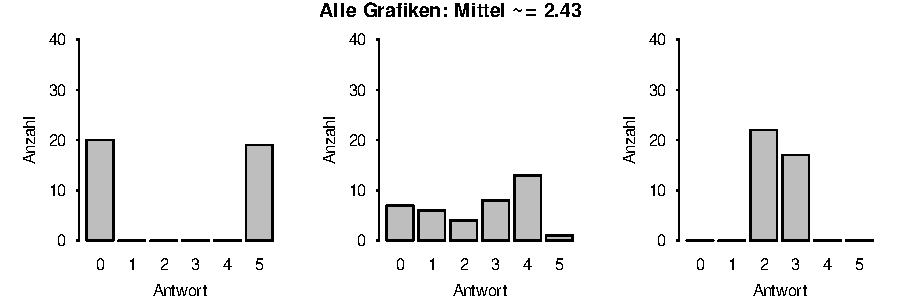
\includegraphics[width=\textwidth]{figs/unnamed-chunk-110-1} 

}

\caption{Hinter dem gleichen Mittelwert kann sich eine Vielzahl von unterschiedlichen Mustern verstecken. Diese drei Grafiken zeigen alle 39 Beobachtungen einer Variablen mit einem Mittel von 2.43 (nach Rundung).\label{fig:samemean}}\label{fig:unnamed-chunk-110}
\end{figure}

\end{knitrout}

Wenn ein Streuuungsmass berichtet wird, schränkt
sich Anzahl möglicher Muster zwar ein, aber trotzdem
können sich hinter einem Mittel und einer Standardabweichung
mehrere Verteilungen verstecken
(Abbildung \ref{fig:samemeansd}).\footnote{Diese Verteilungen wurden generiert anhand des R-Codes unter \url{http://bayesfactor.blogspot.ch/2016/03/how-to-check-likert-scale-summaries-for.html}.}

\begin{knitrout}
\definecolor{shadecolor}{rgb}{0.969, 0.969, 0.969}\color{fgcolor}\begin{figure}[tp]

{\centering 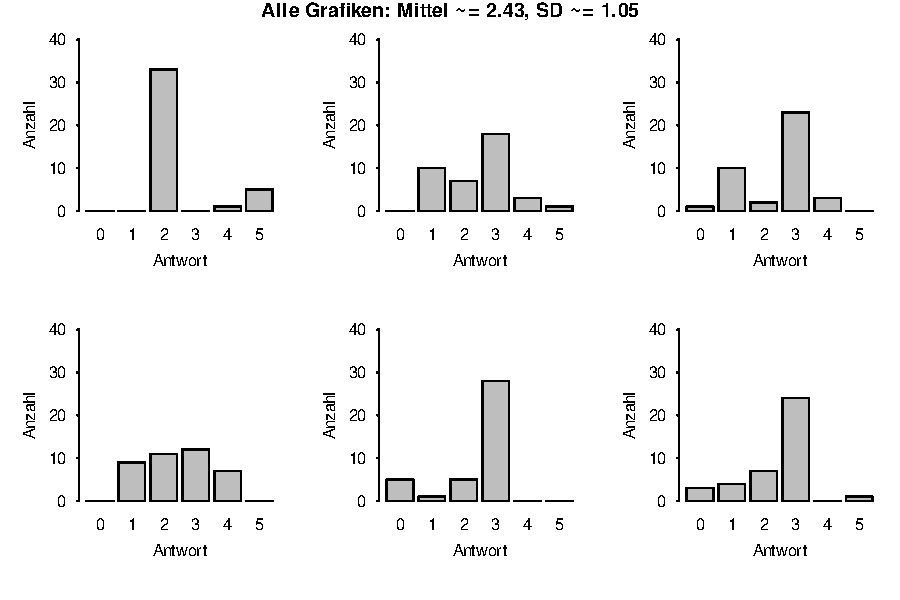
\includegraphics[width=\textwidth]{figs/unnamed-chunk-111-1} 

}

\caption{Sogar wenn man das Mittel und die Standardabweichung kennt, weiss man noch nicht, welches Muster sich hinter diesen Zahlen versteckt. In all diesen Grafiken beträgt das Mittel nach Rundung 2.43 und die Standardabweichung 1.05.\label{fig:samemeansd}}\label{fig:unnamed-chunk-111}
\end{figure}

\end{knitrout}

\medskip

\begin{framed}
\noindent \textbf{Merksatz!} Stellen Sie Ihre Daten auch grafisch dar, sodass Sie und Ihre Leserschaft
wissen, wie diese überhaupt aussehen. Mittelwerte und Streuungsmasse
erzählen nicht die ganze Geschichte.
\end{framed}

\section{Kerndichteschätzungen}
In unserem Norwegischbeispiel gibt es es nur eine geringe Anzahl Beobachtungen
und ausserdem ist die Variable nicht sehr feinkörnig.
Eine sehr feinkörnige Variable wäre eine Variable mit sehr vielen möglichen Ergebnissen
und höchstens einem Beleg pro möglichen Wert.

Was würde nun passieren, wenn
wir eine grosse Anzahl Beobachtungen (z.B.\ 100'000) von einer sehr feinkörnigen
Variablen erheben würden, diese Beobachtungen in einem
Histogramm mit Wahrscheinlichkeitsdichten (siehe Abschnitt \ref{sec:histogram}) darstellen würden
und die Anzahl \textit{bins} immer vergrössern würden?
Wenn die Anzahl \textit{bins} zu gross wird, können wir sie nicht
mehr voneinander unterscheiden, wie Abbildung \ref{fig:density1} zeigt.
Ausserdem werden wir irgendwann nur noch \textit{bins}, die entweder
eine oder keine einzige Beobachtung beinhalten, haben.

\begin{knitrout}
\definecolor{shadecolor}{rgb}{0.969, 0.969, 0.969}\color{fgcolor}\begin{figure}[tp]

{\centering 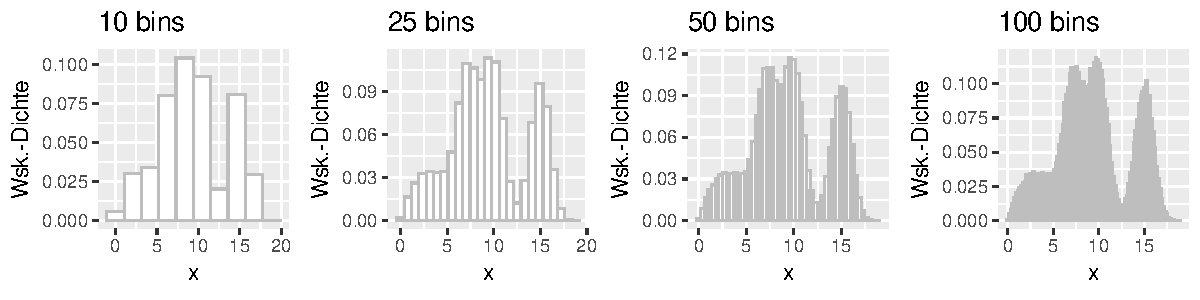
\includegraphics[width=\textwidth]{figs/unnamed-chunk-112-1} 

}

\caption{Vier Histogramme der gleichen feinkörnigen Variablen.\label{fig:density1}}\label{fig:unnamed-chunk-112}
\end{figure}

\end{knitrout}

In solchen Fällen arbeitet man stattdessen mit Kerndichtschätzungen.
Die Berechnungsmethode braucht uns hier nicht zu interessieren; grundsätzlich
handelt es sich um ein geglättetes Histogramm, bei dem die Wahrscheinlichkeitsdichten
jedes Bälkchens mit einer Kurve verbunden werden und die Bälkchen selber nicht mehr dargestellt werden; siehe Abbildung \ref{fig:density2}.

\begin{knitrout}
\definecolor{shadecolor}{rgb}{0.969, 0.969, 0.969}\color{fgcolor}\begin{figure}[tp]

{\centering 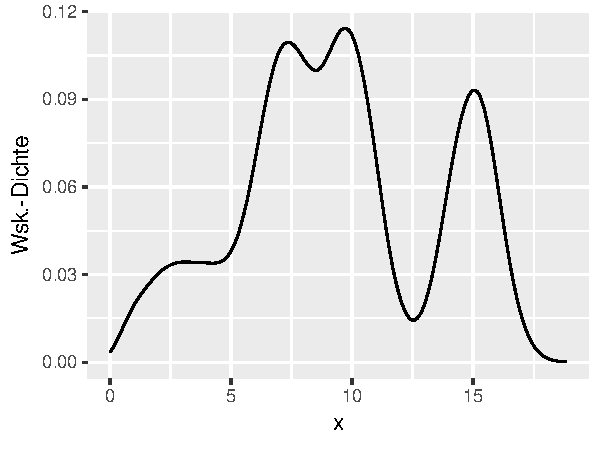
\includegraphics[width=.4\textwidth]{figs/unnamed-chunk-113-1} 

}

\caption{Eine Kerndichteschätzung der gleichen Variablen wie in Abbildung \ref{fig:density1}.\label{fig:density2}}\label{fig:unnamed-chunk-113}
\end{figure}

\end{knitrout}

Achtung! Wahrscheinlichkeitsdichte ist nicht gleich Wahrscheinlichkeit.
In Abbildung \ref{fig:density2} ist die
Wahrscheinlichkeit, dass ein Wert von genau 10
beobachtet wird, nicht fast 12\%, sondern verschwindend gering.
Wenn man bloss genügend Dezimalstellen in Betracht zieht (z.B.\ 10.00000001 oder
9.9999999999), ist jeder einzelne Wert ja verschwindend unwahrscheinlich. Wir können
deswegen keine sinnvollen Wahr\-schein\-lich\-keits\-aus\-sagen über spezifische Werte
machen, sondern nur über Intervalle. Dies machen wir in den nächsten Kapiteln.

Eine Kerndichteschätzung können Sie mit dem Befehl \texttt{geom\_density()} zeichnen; siehe die Beispiele unter \url{https://ggplot2.tidyverse.org/reference/geom_density.html}.
Den Beispielen auf dieser Seite kann man entnehmen, dass man die Kerndichte
einer Variablen auf mehrere Arten schätzen kann, sodass
es nicht \emph{die} Kerndichteschätzung einer bestimmten
Variablen gibt. Vergleichen Sie dazu die erste, dritte und
vierte Grafik, die alle Kerndichteschätzungen der gleichen
Variablen darstellen.

\section{Klassische (idealisierte) Verteilungen}\label{sec:distributions}
Es lassen sich ein paar klassische Arten von Datenverteilungen unterscheiden.
In ihrer reinen Form trifft man diese Verteilungen zwar selten an, aber viele
Datenverteilungen können als Annäherungen dieser Idealisierungen betrachtet werden.

\subsection{Gleichverteilung}
In einer Gleichverteilung (oder Uniformverteilung) ist die
Wahrscheinlichkeitsdichte konstant über dem Bereich der möglichen Werte.
Ein typisches Beispiel ist das Würfeln eines fairen
Würfels (`diskrete Gleichverteilung'; diskret, da es eine
beschränkte Anzahl möglicher
Ergebnisse gibt). Die Wahrscheinlichkeit, eine 6 zu würfeln, ist gleich gross wie
jene, eine 1. usw.\ zu würfeln. Wenn die möglichen Ergebnisse feinkörniger sind,
spricht man von einer `kontinuierlichen Gleichverteilung'.

\begin{knitrout}
\definecolor{shadecolor}{rgb}{0.969, 0.969, 0.969}\color{fgcolor}\begin{figure}[tp]

{\centering 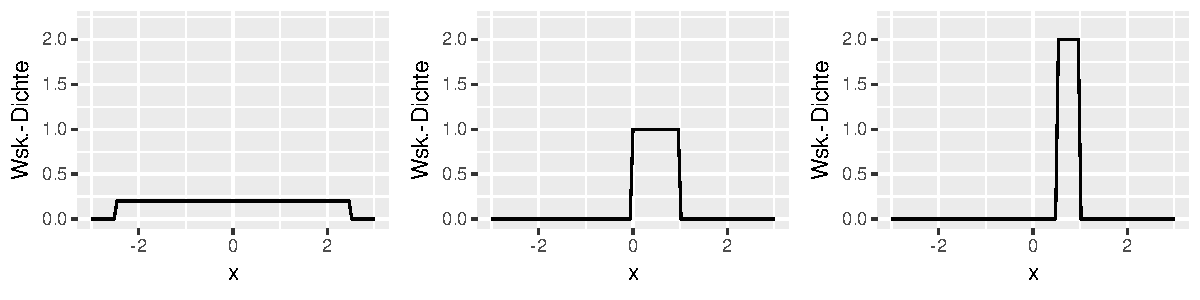
\includegraphics[width=\textwidth]{figs/unnamed-chunk-114-1} 

}

\caption{Wahrscheinlichkeitsdichten von drei kontinuierlichen Gleichverteilungen.\label{fig:uniform}}\label{fig:unnamed-chunk-114}
\end{figure}

\end{knitrout}

\paragraph{Aufgabe.} Abbildung \ref{fig:uniform} zeigt
drei kontinuierliche Gleichverteilungen mit Bereichen [-2.5, 2.5], [0, 1] und [0.5, 1]. Erklären Sie,
warum die Wahrscheinlichkeitsdichte höher als 1 sein kann.

\subsection{Normalverteilung}
Die Normalverteilung ist die typische `Glockenkurve', die man in Statistikbüchern antrifft wie Sand am Meer.
Ihre Wahrscheinlichkeitsdichte wird durch eine kompliziert aussehende Gleichung definiert, die für unsere Zwecke nicht so wichtig ist. Wichtig ist nur, dass die Form der Glockenkurve von zwei Faktoren bestimmt wird: dem Mittel der Datenverteilung ($\mu$) und ihrer Standardabweichung ($\sigma$). $\mu$ bestimmt, um welchen Wert die Kurve zentriert ist; $\sigma$ wie `breit' und `hoch' die Kurve ist.
Siehe Abbildung \ref{fig:normal}.

\begin{knitrout}
\definecolor{shadecolor}{rgb}{0.969, 0.969, 0.969}\color{fgcolor}\begin{figure}[tp]

{\centering 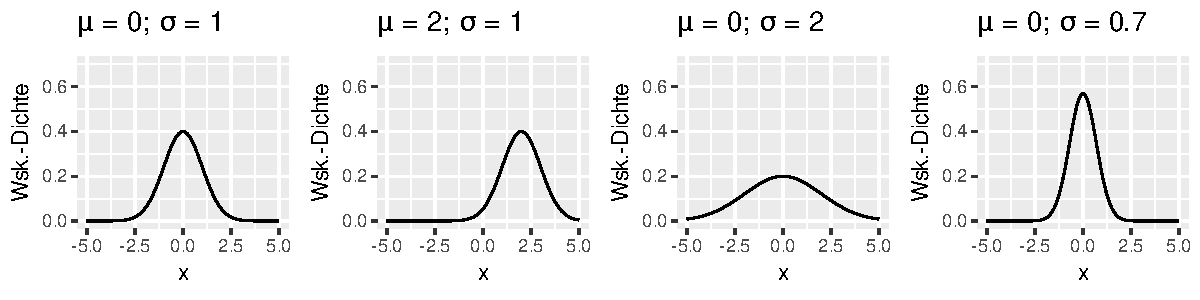
\includegraphics[width=\textwidth]{figs/unnamed-chunk-115-1} 

}

\caption{Die Form einer Normalverteilung ist von zwei Parametern abhängig: ihrem Mittel ($\mu$) und ihrer Standardabweichung ($\sigma$).\label{fig:normal}}\label{fig:unnamed-chunk-115}
\end{figure}

\end{knitrout}

Gleichverteilungen und Normalverteilungen sind Beispiele von \textbf{symmetrischen Verteilungen}: Die linke Hälfte der Verteilung formt
das Spiegelbild der rechten Hälfte. Bei Variablen, die symmetrisch verteilt sind, sind das Mittel und der Median einander (ungefähr) gleich.

% Bei einer Normalverteilung sind Modus, Mittel und Median gleich,
% d.h., es gibt eine eindeutige zentrale Tendenz.
% Mit vielen statistischen Verfahren kann man Aussagen über das
% Mittel einer Population oder Stichprobe machen.
% Wenn Mittel, Median und Modus alle (mehr oder weniger) gleich sind---wie bei Normalverteilungen---,
% kann man mit diesen Verfahren die zentrale Tendenz also völlig erfassen.
% Wenn die Daten stark von einer Normalverteilung abweichen,
% können die Aussagen, die solche Verfahren übers Mittel machen, zwar noch stimmen.
% Sie sind aber eben weniger relevant fürs Erfassen der zentralen Tendenz:
% Das Mittel ist ja bloss ein Versuch, die zentrale Tendenz zu erfassen.
% Manchmal sind Daten zwar nicht-normalverteilt,
% können aber einfach zu annähernd normalverteilten
% Daten \textbf{transformiert} werden.
% Solche Datentransformationen werden in diesem Skript
% nur oberflächlich behandelt;
% siehe aber \citet[][S.~59--68]{Gelman2007}
% und \citet{Baayen2010}.

% Wie wir in den nächsten Kapiteln sehen werden,
% ist die Normalverteilung auch aus anderen Gründen
% in der Statistik von zentraler Bedeutung:
% Eine Reihe mathematischer Sätze,
% die die Analyse vereinfachen, gilt nur nachweisbar,
% wenn die Daten aus einer Normalverteilung stammen.

% % Es ist aus diesen Gründen praktisch,
% % überprüfen zu können, ob die Daten, die man ge
% % ob Daten annähernd normalverteilt sind.
% % Manchmal werden zu diesem Zweck statistische Tests verwendet, aber diese würde ich nicht empfehlen.
% % Beispiele sind der Shapiro--Wilk-Test (\texttt{?shapiro.test}) und der Kolmogorov--Smirnov-Test (\texttt{?ks.test}).
% % Ein erster Grund, weshalb ich solche numerischen Tests nicht empfehle, ist, dass sie sehr
% % von der Stichprobengrösse abhängig sind: Grobe Verletzungen gegen Normalität werden in kleinen
% % Stichproben nicht identifiziert, während in grossen Stichproben sogar die kleinsten Verletzungen
% % als problematisch bezeichnet werden. Dabei ist es für die häufigsten statistischen Verfahren
% % gerade bei grösseren Stichproben weniger wichtig, dass die Daten normalverteilt sind.
% % Der zweite Grund ist, dass Ihre Leserschaft sich vermutlich weniger gut mit solchen Tests auskennt.
% % Ich erwähne diese Tests nur, weil man sie in Forschungsartikeln öfters antrifft und nicht weil man sich selber auf sie verlassen sollte.q}
% % Vielmehr sollte man sich auf eine visuelle Dateninspektion verlassen: Zeichnen Sie Histogramme und Wahrscheinlichkeitsdichten.
% \end{mdframed}
%
\subsection{Bimodale Verteilung}
Eine bimodale Verteilung ist eine Verteilung mit zwei `Höckern'.
Bei einer Befragung zu einem gesellschaftlichen Thema etwa
würde eine solche Verteilung darauf hindeuten,
dass die Bevölkerung stark zwischen Befürwortern und Gegnern polarisiert ist
und dass relativ wenige Leute eine Zwischenposition vertreten.
Eine bimodale Verteilung kann auch darauf hindeuten,
dass eigentlich zwei Populationen statt nur einer gemessen wurden.
Zum Beispiel ist (in der akustischen Phonetik) die Verteilung der Grundfrequenz in der ganzen Population bimodal verteilt: Männerstimmen haben
eine tiefere Grundfrequenz als Frauenstimmen, aber innerhalb jeder Gruppe sind die Werte ungefähr normalverteilt.

Manchmal trifft man auch \textbf{multimodale} Verteilungen,
also Verteilungen mit mehreren Höckern, an.

Bi- und multimodale Verteilungen können zwar symmetrisch sein,
und folglich können das Mittel und der Median einander recht ähnlich
sein. Trotzdem zeigen diese Mittelwerte nicht, welche Werte typisch
für solche Verteilungen sind. Wenn eine bimodale Verteilung in separate
Populationen zerteilt werden kann (z.B.\ Männer und Frauen), ist es
sinnvoller, die Mittelwerte innerhalb jeder Population zu berechnen.
Wenn dies unmöglich ist, dürfte es sinnvoller sein, die Verteilung grafisch
zu berichten (immer eine gute Idee!) oder sie in Vollsätzen
zu beschreiben anstatt einen sinnlosen Mittelwert zu berechnen.

\subsection{Schiefe Verteilungen}
Eine \textbf{rechtsschiefe Verteilung} (oder: Verteilung mit positiver Schiefe)
ist eine Verteilung, die nicht symmetrisch ist, sondern nach rechts neigt.
Etwa Reaktionszeiten, Wortfrequenzen und die Anzahl tip-of-the-tongue-Probleme pro Aufnahme sind oft rechtsschief verteilt: Die meisten Reaktionszeiten sind niedrig,
aber einige werden hoch sein; die allermeisten Wörter kommen selten vor, aber eine
Handvoll Wörter sehr häufig; in den meisten Aufnahmen wird es keine tip-of-the-tongue-Probleme geben, aber in ein paar schon einige.

Eine \textbf{linksschiefe Verteilung} (oder: Verteilung mit negativer Schiefe) ist nicht-sym\-me\-trisch und neigt nach links.
Bei Testergebnissen könnte dies darauf hindeuten, dass der Test zu einfach war (\textbf{Deckeneffekt}): Personen mit dem gleichen hohen Testergebnis unterscheiden sich vermutlich noch voneinander in ihrer Fähigkeit, aber dies zeigt sich aufgrund des zu einfachen Tests nicht.
Zu schwierige Tests führen hingegen zu rechtsschiefen Verteilungen (\textbf{Bodeneffekt}).

Bei schiefen Verteilungen können Mittel und Median weit auseinander liegen
und es ist durchaus möglich, dass keiner der beiden Werte den typischen
Wert der Verteilung wirklich erfasst.

Abbildung \ref{fig:other} zeigt eine bimodale, eine rechtsschiefe und eine linksschiefe Verteilung.

\begin{knitrout}
\definecolor{shadecolor}{rgb}{0.969, 0.969, 0.969}\color{fgcolor}\begin{figure}[tp]

{\centering 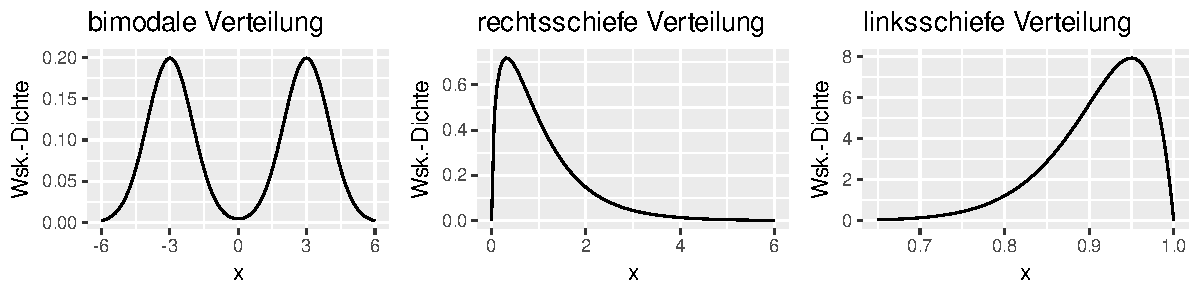
\includegraphics[width=.8\textwidth]{figs/unnamed-chunk-116-1} 

}

\caption{Eine bimodale und zwei schiefe Verteilungen.\label{fig:other}}\label{fig:unnamed-chunk-116}
\end{figure}

\end{knitrout}

\section{Weiterführende Literatur}
\citet{Huff1954} (\textit{How to lie with statistics})
ist ein kurzes und sehr lesbares Büchlein. Es behandelt
unter anderem die unterschiedlichen Mittelwerte und wie
diese manipulativ eingesetzt werden.

\citet{Johnson2013} bietet eine Übersicht über weitere
Möglichkeiten, Daten grafisch und numerisch zu beschreiben.

In diesem Skript werden zwar mehrere nützliche Arten von
Grafiken vorgestellt, aber eine ausführlichere Behandlung
finden Sie bei \citet{Healy2019}. Dieses Buch ist auch
kostenlos verfügbar unter \url{https://socviz.co/}.

\section{Aufgaben}

\begin{enumerate}

  \item Es sei $x$ der folgende Vektor: $(4, 2, 1, 5, 4)$.
  Berechnen Sie die folgenden Summen von Hand:
  \begin{enumerate}
   \item $\sum_{i=1}^5 x_i$;
   \item $\sum_{j=2}^3 x_j$;
   \item $\sum_{i=2}^4 (x_i + 2)$;
   \item $\sum_{i=2}^4 (3x_i - 2)$;
   \item $\sum_{i=2}^4 \frac{10}{x_i}$;
   \item $\sum_{i=1}^6 i$;
   \item $\sum_{i=2}^4 3$;
   \item $\sum_{i=1}^2 x_{2i}$;
   \item $\sum_{i=1}^2 (x_{2i} - x_{2i-1})$.
  \end{enumerate}

  \item Erklären Sie, ohne den Code auszuführen, was dieser Codeabschnitt bewirkt
  und was sein Output wäre.

\begin{knitrout}
\definecolor{shadecolor}{rgb}{0.969, 0.969, 0.969}\color{fgcolor}\begin{kframe}
\begin{alltt}
\hlstd{> }\hlstd{werte} \hlkwb{<-} \hlkwd{vector}\hlstd{(}\hlkwc{length} \hlstd{=} \hlnum{20}\hlstd{)}
\hlstd{> }\hlstd{werte[[}\hlnum{1}\hlstd{]]} \hlkwb{<-} \hlnum{1}
\hlstd{> }\hlstd{werte[[}\hlnum{2}\hlstd{]]} \hlkwb{<-} \hlnum{1}
\hlstd{> }\hlkwa{for} \hlstd{(i} \hlkwa{in} \hlnum{3}\hlopt{:}\hlkwd{length}\hlstd{(werte)) \{}
\hlstd{+ }  \hlstd{werte[[i]]} \hlkwb{<-} \hlstd{werte[[i}\hlopt{-}\hlnum{1}\hlstd{]]} \hlopt{+} \hlstd{werte[[i}\hlopt{-}\hlnum{2}\hlstd{]]}
\hlstd{+ }\hlstd{\}}
\hlstd{> }\hlstd{werte[[}\hlnum{6}\hlstd{]]}
\end{alltt}
\end{kframe}
\end{knitrout}

% 
%   \item Das durchschnittliche Einkommen per Gemeinde wird
%   üblicherweise mit dem Median statt mit dem Mittel ausgedrückt. Warum?

  \item 80 willkürlich ausgewählte Schweizer Staatsbürger werden gebeten, auf einer 10er-Skala anzudeuten,
  inwieweit sie mit der Aussage \textit{Privater Waffenbesitz sollte verboten werden} einverstanden sind
  (1 = gar nicht einverstanden; 10 = völlig einverstanden).
  Würde diese Befragung annähernd normalverteilte Daten liefern?
  Wenn nicht, welcher Datenverteilung würden sie am ehesten entsprechen?
%
%   \item M{\&}Ms können sechs Farben haben: blau, braun, gelb, grün, orange und rot.
%   Wie schätzen Sie die relativen Frequenzen dieser Farben ein?
%   Gibt es z.B.\ Ihrer Erfahrung nach eine ähnlich grosse Anzahl blaue wie rote M{\&}Ms?
%   Entspricht diese Verteilung einer der Verteilungen, die wir oben kennengelernt haben?

  \item Die Datei \texttt{stocker2017.csv} enthält einen Teil der Daten aus einer
  on-line-Studie von \citet{Stocker2017}.
  160 Versuchspersonen wurden gebeten, die Glaubwürdigkeit von Aussagen von
  SprecherInnen mit unterschiedlichen Akzenten (Englisch, Französisch, Deutsch und Italienisch)
  mithilfe eines \textit{sliders} auf einer Skala von 0 bis 100 zu bewerten.
  Diese Daten stehen in der \texttt{score}-Spalte.\label{ex:stocker}

    \begin{enumerate}
      \item Lesen Sie diese Datei in R ein. Kontrollieren Sie, ob dies geklappt hat.

      \item Berechnen Sie das Mittel und den Median der \texttt{score}-Daten.
      Sind sich diese Mittelwerte ähnlich?

      \item Stellen Sie die \texttt{score}-Daten in einem Histogramm mit 10 \textit{bins} dar.
      Welcher klassischen Verteilung entspricht diese am ehesten?

      \item Zeichnen Sie ein Histogramm mit 100 bins.
      Beschreiben Sie dieses Histogramm.
      Sind das Mittel und der Median repräsentativ für diese Daten?

      \item Welcher Wert ist der dritthäufigste? Warum, denken Sie?

      \item Was ist bei den viert-, fünft-, sechst- usw. -häufigsten Werten auffällig?
    \end{enumerate}
    
    \item Es sei $x = (x_1, x_2, \dots, x_n)$ ein Vektor
    mit strikt positiven Zahlen. Das \textbf{harmonische Mittel}
    $H$ dieser Zahlen ist nun definiert als
    \[
      H = \frac{n}{\sum_{i=1}^n \frac{1}{x_i}}.
    \]
    Schreiben Sie eine eigene R-Funktion \texttt{harmonic\_mean()},
    welche einen Vektor mit einer beliebigen Anzahl strikt positiver
    Zahlen als Parameter erhält und sein harmonisches Mittel ausspuckt.

    
    Hinweis: Wenn Sie den ersten Kilometer gegen 5 Kilometer/Stunde
    überbrücken, den zweiten gegen 10 Kilometer/Stunde
    und den dritten gegen 2 Kilometer/Stunde, dann haben Sie insgesamt
    3 Kilometer in 48 Minuten überbrückt. (Man rechne nach.)
    Dies entspricht einer durchschnittlichen Geschwindigkeit von 3.75
    Kilometer/Stunde.
    Diese durchschnittliche Geschwindigkeit können
    Sie mit dem harmonischen Mittel berechnen. Wenn Ihre Funktion
    gut geschrieben ist, sollte der folgende Befehl die Antwort 3.75 ergeben:
\begin{knitrout}
\definecolor{shadecolor}{rgb}{0.969, 0.969, 0.969}\color{fgcolor}\begin{kframe}
\begin{alltt}
\hlstd{> }\hlkwd{harmonic_mean}\hlstd{(}\hlkwd{c}\hlstd{(}\hlnum{5}\hlstd{,} \hlnum{10}\hlstd{,} \hlnum{2}\hlstd{))}
\end{alltt}
\begin{verbatim}
[1] 3.75
\end{verbatim}
\end{kframe}
\end{knitrout}


\end{enumerate}


\chapter{Wahrscheinlichkeitsaussagen über Zufallsvariablen}\label{ch:wahrscheinlichkeiten}

Dieses Kapitel dient als Auffrischung der Wahrscheinlichkeitsrechnung.
Konkret besprechen wir, wie wir Wahrscheinlichkeitsaussagen über 
\textbf{Zufallsvariablen} machen können, wenn wir schon wissen, 
aus welcher Verteilung diese Variable stammt. Was Zufallsvariablen
sind, wird aus den Beispielen klar. Die Fähigkeit, 
Wahrscheinlichkeitsaussagen über Zufallsvariablen zu machen, 
ist an sich schon praktisch, aber zudem muss man die 
hinterliegende Logik kennen, wenn man Inferenzstatistik verstehen will.

\section{Beispiel: kontinuierliche Gleichverteilung}\label{sec:continuousuniform}
Die Kreislinie eines Rads ist wie in Abbildung \ref{fig:kreis} 
mit Zahlen von 0 bis 360 vermerkt. Jedes Mal, wenn der Pfeil 
gedreht wird, bleibt er an einer zufälligen Stelle auf der 
Kreislinie stehen. Dies entspricht einer kontinuierlichen 
Gleichverteilung mit einem Bereich von 0 bis 360; siehe Abbildung
\ref{fig:kreisdichte}.
Da die Verteilung von 0 bis 360 geht und die Fläche zwischen der Wahrscheinlichkeitsdichte und der $x$-Achse 1 betragen muss,
ist die Wahrscheinlichkeitsdichte überall $\frac{1}{360} \approx 0.0028$,
denn $(360-0) \cdot \frac{1}{360} = 1$.

\begin{figure}[tp]
\begin{center}
  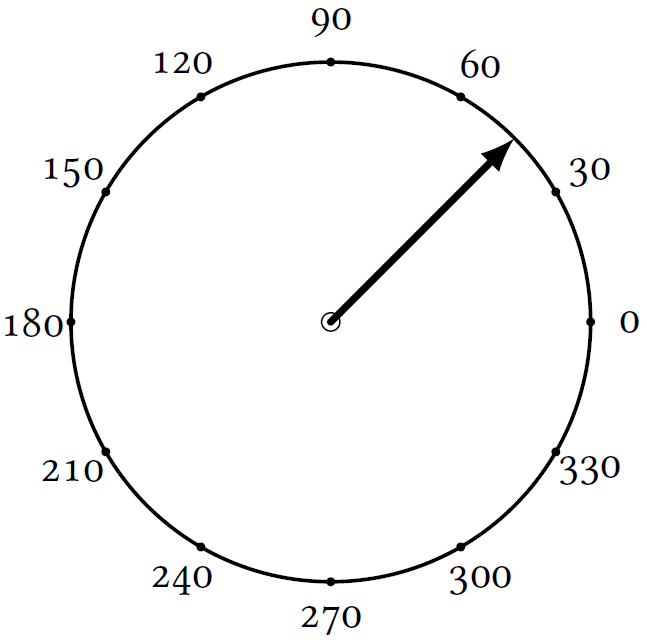
\includegraphics[width = .33\textwidth]{figs/kreis}
\caption{Ein Rad mit einem Pfeil, um eine Gleichverteilung zu generieren.}
\label{fig:kreis}
\end{center}
\end{figure}

\begin{knitrout}
\definecolor{shadecolor}{rgb}{0.969, 0.969, 0.969}\color{fgcolor}\begin{figure}[tp]

{\centering 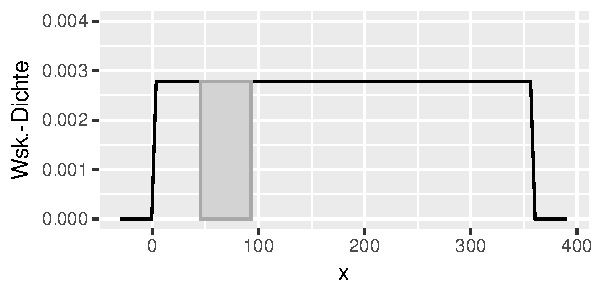
\includegraphics[width=.5\textwidth]{figs/unnamed-chunk-120-1} 

}

\caption{Wahrscheinlichkeitsdichte einer kontinuierlichen Gleichverteilung mit Bereich 0 bis 360.\label{fig:kreisdichte}}\label{fig:unnamed-chunk-120}
\end{figure}

\end{knitrout}

\subsection{Wahrscheinlichkeit = Fläche unter der Wahrscheinlichkeitsdichte}
Wie wahrscheinlich ist es, dass wir den Pfeil drehen und er irgendwo
zwischen 45 und 93 stehen bleibt? Zwischen den Werten 45 und 93
liegt etwa 13.3\% der ganzen  Wahrscheinlichkeitsverteilung:
$\frac{93-45}{360} = 0.133$.
Die Wahrscheinlichkeit liegt also bei 13.3\%.

Diese Berechnungsmethode lässt sich aber nur bei Gleichverteilungen
anwenden, also bei Verteilungen, bei denen jeder Wert genauso
wahrscheinlich ist. Eine Methode, die auch für andere Verteilungen
gilt, besteht darin, \textbf{die Fläche unter der Wahrscheinlichkeitsdichte
zwischen den beiden Werten} -- das `Integral' aus dem Gymnasium -- zu berechnen.
Diese Fläche wurde in der obigen Grafik grau eingefärbt.
Bei einer Gleichverteilung ist dies ein Rechteck, dessen Fläche wir einfach berechnen können: $\textrm{Breite} \cdot \textrm{Höhe} = (93-45) \cdot \frac{1}{360} = 0.133$.

\subsection{Kumulative Verteilungsfunktion}
Abbildung \ref{fig:uniformcumulative} zeigt,
wie wahrscheinlich es ist, einen Wert kleiner als $x$ zu beobachten.
Diese Grafik nennt man eine
\textbf{kumulative Verteilungsfunktion};
die kumulative Wahrscheinlichkeit variiert von 0 bis 1.

\begin{knitrout}
\definecolor{shadecolor}{rgb}{0.969, 0.969, 0.969}\color{fgcolor}\begin{figure}[tp]

{\centering 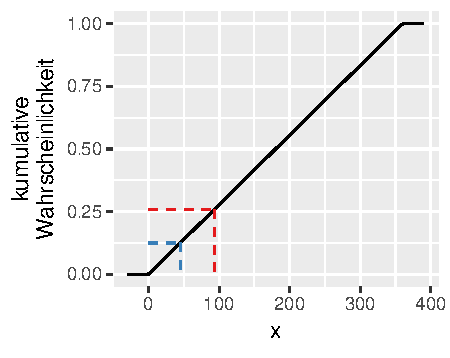
\includegraphics[width=.33\textwidth]{figs/unnamed-chunk-121-1} 

}

\caption{Kumulative Verteilungsfunktion einer kontinuierlichen Gleichverteilung mit Bereich 0 bis 360.\label{fig:uniformcumulative}}\label{fig:unnamed-chunk-121}
\end{figure}

\end{knitrout}

Mit \texttt{punif()} können wir die Wahrscheinlichkeit
berechnen, dass wir einen Wert zwischen 45 und 93 beobachten
(\textit{p} für \textit{probability},
\textit{unif} für \textit{uniform distribution}).
Zuerst berechnen wir die Wahrscheinlichkeit, dass wir einen
Wert kleiner als 93 beobachten. Diese Wahrscheinlichkeit
entspricht dem Wert auf der $y$-Achse für die rote Linie
in Abbildung \ref{fig:uniformcumulative}
(Handgelenk mal Pi: etwa 25\%). Mit \texttt{punif()} berechnen
wir die genaue Wahrscheinlichkeit, dass man einen Wert
niedriger als 93 antrifft, wenn die Verteilung eine Gleichverteilung
zwischen 0 und 360 ist:
\begin{knitrout}
\definecolor{shadecolor}{rgb}{0.969, 0.969, 0.969}\color{fgcolor}\begin{kframe}
\begin{alltt}
\hlstd{> }\hlkwd{punif}\hlstd{(}\hlnum{93}\hlstd{,} \hlkwc{min} \hlstd{=} \hlnum{0}\hlstd{,} \hlkwc{max} \hlstd{=} \hlnum{360}\hlstd{)}
\end{alltt}
\begin{verbatim}
[1] 0.25833
\end{verbatim}
\end{kframe}
\end{knitrout}

Ebenso können wir die Wahrscheinlichkeit berechnen,
dass wir einen Wert kleiner als 45 beobachten (blau):
\begin{knitrout}
\definecolor{shadecolor}{rgb}{0.969, 0.969, 0.969}\color{fgcolor}\begin{kframe}
\begin{alltt}
\hlstd{> }\hlkwd{punif}\hlstd{(}\hlnum{45}\hlstd{,} \hlkwc{min} \hlstd{=} \hlnum{0}\hlstd{,} \hlkwc{max} \hlstd{=} \hlnum{360}\hlstd{)}
\end{alltt}
\begin{verbatim}
[1] 0.125
\end{verbatim}
\end{kframe}
\end{knitrout}

Der Unterschied ist die Wahrscheinlichkeit, dass
wir einen Wert zwischen 45 und 93 beobachten:
\begin{knitrout}
\definecolor{shadecolor}{rgb}{0.969, 0.969, 0.969}\color{fgcolor}\begin{kframe}
\begin{alltt}
\hlstd{> }\hlnum{0.2583} \hlopt{-} \hlnum{0.125}
\end{alltt}
\begin{verbatim}
[1] 0.1333
\end{verbatim}
\begin{alltt}
\hlstd{> }\hlcom{# oder direkt:}
\hlstd{> }\hlkwd{punif}\hlstd{(}\hlnum{93}\hlstd{,} \hlkwc{min} \hlstd{=} \hlnum{0}\hlstd{,} \hlkwc{max} \hlstd{=} \hlnum{360}\hlstd{)} \hlopt{-} \hlkwd{punif}\hlstd{(}\hlnum{45}\hlstd{,} \hlkwc{min} \hlstd{=} \hlnum{0}\hlstd{,} \hlkwc{max} \hlstd{=} \hlnum{360}\hlstd{)}
\end{alltt}
\begin{verbatim}
[1] 0.13333
\end{verbatim}
\end{kframe}
\end{knitrout}

\section{Beispiel Normalverteilung}
IQ-Werte sind normalverteilt mit---per Definition---Mittel 100
und Standardabweichung 15. Abbildung \ref{fig:iqdistribution}
zeigt die Wahrscheinlichkeitsdichte und die kumulative
Wahrscheinlichkeit dieser Normalverteilung.

\begin{knitrout}
\definecolor{shadecolor}{rgb}{0.969, 0.969, 0.969}\color{fgcolor}\begin{figure}[tp]

{\centering 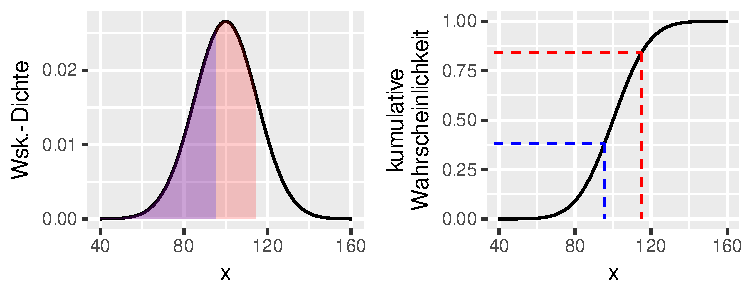
\includegraphics[width=.7\textwidth]{figs/unnamed-chunk-125-1} 

}

\caption{Wahrscheinlichkeitsdichte und kumulative Wahrscheinlichkeit einer Normalverteilung mit Mittel 100 und Standardabweichung 15.\label{fig:iqdistribution}}\label{fig:unnamed-chunk-125}
\end{figure}

\end{knitrout}

Wenn wir zufällig eine Person aus der Gesamtpopulation wählen,
wie wahrscheinlich ist es dann, dass ihr IQ niedriger als 115 ist?
Diese Wahrscheinlichkeit entspricht der Fläche unter
der Wahrscheinlichkeitsdichte zwischen $-\infty$ (minus unendlich) und 115;
diese Fläche wurde in der linken Grafik rötlich eingefärbt.
Mit der \texttt{pnorm()}-Funktion können wir diesen Wert genau berechnen
(roter Wert in der rechten Grafik; visuell geschätzt: 85\%):
\begin{knitrout}
\definecolor{shadecolor}{rgb}{0.969, 0.969, 0.969}\color{fgcolor}\begin{kframe}
\begin{alltt}
\hlstd{> }\hlkwd{pnorm}\hlstd{(}\hlnum{115}\hlstd{,} \hlkwc{mean} \hlstd{=} \hlnum{100}\hlstd{,} \hlkwc{sd} \hlstd{=} \hlnum{15}\hlstd{)}
\end{alltt}
\begin{verbatim}
[1] 0.84134
\end{verbatim}
\end{kframe}
\end{knitrout}

Die Wahrscheinlichkeit, dass eine zufällig ausgewählte Person
einen IQ von 115 oder niedriger hat liegt also bei 84\%.

Mit der Option \texttt{lower.tail = FALSE} können wir das Komplement
dieses Werts berechnen, d.h., die Wahrscheinlichkeit, einen Wert höher
als 115 anzutreffen:
\begin{knitrout}
\definecolor{shadecolor}{rgb}{0.969, 0.969, 0.969}\color{fgcolor}\begin{kframe}
\begin{alltt}
\hlstd{> }\hlkwd{pnorm}\hlstd{(}\hlnum{115}\hlstd{,} \hlkwc{mean} \hlstd{=} \hlnum{100}\hlstd{,} \hlkwc{sd} \hlstd{=} \hlnum{15}\hlstd{,} \hlkwc{lower.tail} \hlstd{=} \hlnum{FALSE}\hlstd{)}
\end{alltt}
\begin{verbatim}
[1] 0.15866
\end{verbatim}
\begin{alltt}
\hlstd{> }\hlcom{# oder:}
\hlstd{> }\hlnum{1} \hlopt{-} \hlkwd{pnorm}\hlstd{(}\hlnum{115}\hlstd{,} \hlkwc{mean} \hlstd{=} \hlnum{100}\hlstd{,} \hlkwc{sd} \hlstd{=} \hlnum{15}\hlstd{)}
\end{alltt}
\begin{verbatim}
[1] 0.15866
\end{verbatim}
\end{kframe}
\end{knitrout}

Wir können die Frage auch andersherum stellen,
z.B.: Für welchen IQ-Wert gilt, dass 38\% der Population einen
niedrigeren IQ haben? Hierzu verwenden wir die
\texttt{qnorm()}-Funktion (\textit{q} für \textit{quantile};
blauer $x$-Wert in der obigen Grafik):
\begin{knitrout}
\definecolor{shadecolor}{rgb}{0.969, 0.969, 0.969}\color{fgcolor}\begin{kframe}
\begin{alltt}
\hlstd{> }\hlkwd{qnorm}\hlstd{(}\hlnum{0.38}\hlstd{,} \hlkwc{mean} \hlstd{=} \hlnum{100}\hlstd{,} \hlkwc{sd} \hlstd{=} \hlnum{15}\hlstd{)}
\end{alltt}
\begin{verbatim}
[1] 95.418
\end{verbatim}
\end{kframe}
\end{knitrout}

38\% der Population hat also einen IQ niedriger als 95.4.
Anders gesagt: Das 38.\ \textbf{Perzentil} der IQ-Verteilung
(einer Normalverteilung mit Mittel 100 und einer Standardabweichung von 15) ist 95.4.

Eine andere Frage könnte sein: Zwischen welchen zwei Werten, die symmetrisch
um das Mittel liegen, befinden sich 80\% der IQ-Werte in der Population?
Symmetrisch ums Mittel liegen 80\% der Daten zwischen dem 10.\ und 90.\ Perzentil, daher:
\begin{knitrout}
\definecolor{shadecolor}{rgb}{0.969, 0.969, 0.969}\color{fgcolor}\begin{kframe}
\begin{alltt}
\hlstd{> }\hlkwd{qnorm}\hlstd{(}\hlnum{0.10}\hlstd{,} \hlkwc{mean} \hlstd{=} \hlnum{100}\hlstd{,} \hlkwc{sd} \hlstd{=} \hlnum{15}\hlstd{)}
\end{alltt}
\begin{verbatim}
[1] 80.777
\end{verbatim}
\begin{alltt}
\hlstd{> }\hlkwd{qnorm}\hlstd{(}\hlnum{0.90}\hlstd{,} \hlkwc{mean} \hlstd{=} \hlnum{100}\hlstd{,} \hlkwc{sd} \hlstd{=} \hlnum{15}\hlstd{)}
\end{alltt}
\begin{verbatim}
[1] 119.22
\end{verbatim}
\end{kframe}
\end{knitrout}
Oder mithilfe der \texttt{c()}-Funktion:
\begin{knitrout}
\definecolor{shadecolor}{rgb}{0.969, 0.969, 0.969}\color{fgcolor}\begin{kframe}
\begin{alltt}
\hlstd{> }\hlkwd{qnorm}\hlstd{(}\hlkwd{c}\hlstd{(}\hlnum{0.10}\hlstd{,} \hlnum{0.90}\hlstd{),} \hlkwc{mean} \hlstd{=} \hlnum{100}\hlstd{,} \hlkwc{sd} \hlstd{=} \hlnum{15}\hlstd{)}
\end{alltt}
\begin{verbatim}
[1]  80.777 119.223
\end{verbatim}
\end{kframe}
\end{knitrout}

\section{Aufgaben}\label{sec:uebungenprobability}

Die folgenden Übungen dienen dazu,
Sie mit dem Rechnen mit Wahrscheinlichkeiten und mit
den \texttt{p...()}- und \texttt{q...()}-Funktionen 
besser vertraut zu machen.

\begin{enumerate}

\item M{\&}Ms kommen in sechs Farben vor; in Tabelle \vref{tab:mandms} werden ihre relativen Frequenzen aufgelistet. (Für diese Übungen brauchen Sie nicht mit R zu arbeiten.)

\begin{enumerate}
\item Wie wahrscheinlich ist es, dass ein zufällig ausgewähltes M{\&}M rot \emph{oder} orange ist?
\item Wie wahrscheinlich ist es, dass zwei zufällig ausgewählte M{\&}Ms \emph{beide} rot oder orange (also zwei rote, zwei orange oder ein rotes und ein oranges) sind?
\item Wie wahrscheinlich ist es, dass von zwei zufällig ausgewählten M{\&}Ms ein rotes und ein oranges dabei sind?
\item Wie wahrscheinlich ist es, dass wenn 5 M{\&}Ms zufällig ausgewählt werden, alle blau sind?
\item Wie wahrscheinlich ist es, dass wenn 5 M{\&}Ms zufällig ausgewählt werden, kein einziges blau ist?\label{ex:mm}
\end{enumerate}

\begin{table}[tbp]
\centering
\caption{Relative Frequenzen von M\&Ms nach Farbe.}
\label{tab:mandms}
\begin{tabular}{@{}lr@{}}
\toprule
Farbe  & relative Frequenz \\ \midrule
blau   & 23\%              \\
orange & 23\%              \\
gelb   & 15\% \\
grün   & 15\% \\
braun  & 12\% \\
rot    & 12\% \\
\bottomrule
\end{tabular}
\end{table}

\item In diesem Kapitel haben Sie die IQ-Verteilung kennengelernt.
\begin{enumerate}
\item Wie wahrscheinlich ist es, dass eine zufällig ausgewählte Person einen IQ niedriger als 90 hat?
\item Wie wahrscheinlich ist es, dass eine zufällig ausgewählte Person einen IQ grösser als 85 hat?
\item Wie wahrscheinlich ist es, dass eine zufällig ausgewählte Person einen IQ zwischen 110 und 120 hat?
\item Wie wahrscheinlich ist es, dass eine zufällig ausgewählte Person einen IQ hat, der mehr als zwei Standardabweichungen vom Populationsmittel entfernt liegt?
\item Durchschnittliche Intelligenz ist definiert als der IQ der mittleren 45\% der Bevölkerung. Zwischen welchen zwei Werten liegt er?
\item Die folgenden Übungen sind etwas schwieriger und haben als Ziel, Sie über kombinierte Wahrscheinlichkeiten nachdenken zu lassen.\\
Wie wahrscheinlich ist es, dass, wenn zwei Personen zufällig ausgewählt werden, keine der beiden einen IQ niedriger als 105 hat?\\
(Tipp: Wie wahrscheinlich ist es, dass eine einzige Person einen IQ höher als 105 hat?)
\item Wie wahrscheinlich ist es, dass, wenn drei Personen zufällig ausgewählt werden, \emph{genau} eine Person einen IQ niedriger als 90 hat?\\
(Tipp: Wie wahrscheinlich ist es, dass die erste Person einen IQ niedriger als 90 hat, die zweite und die dritte aber nicht? Was ist nun die Wahrscheinlichkeit, dass die zweite Person einen IQ niedriger als 90 hat, die erste und die dritte aber nicht? Und wie wahrscheinlich ist es, dass die dritte Person einen IQ niedriger als 90 hat, die ersten zwei aber nicht?)
\item Wie wahrscheinlich ist es, dass, wenn drei Personen zufällig ausgewählt werden, \emph{mindestens} eine Person einen IQ niedriger als 90 hat?\\
(Tipp: Wie wahrscheinlich ist es, dass keine einzige Person einen IQ niedriger als 90 hat?)
\end{enumerate}

\item Wie wahrscheinlicht ist es, bei einer normalverteilten Variable (\emph{egal welcher!}) einen zufällig ausgewählten Wert, der weniger als 1; 1,5; und 2 Standardabweichungen vom Mittel entfernt ist, anzutreffen?\\
(Tipp: Zeichnen Sie ein paar Normalverteilungen mit anderen Mitteln und Standardabweichungen und beantworten Sie diese Frage für jede Verteilung separat.)

\item Poker wird mit 52 Spielkarten gespielt: 13 Werte (2, 3, \dots, Bube, Dame, König, Ass) in vier Farben (Kreuz, Pik, Herz und Karo).
\begin{enumerate}
\item Wie wahrscheinlich ist es, dass eine zufällig ausgewählte Karte ein Ass ist?
\item Sie ziehen zufällig zwei Karten aus dem Blatt. Die erste Karte ist ein Ass. Wie wahrscheinlich ist es, dass auch die zweite Karte ein Ass ist?
\item Sie ziehen zufällig eine Karte aus dem Blatt, schauen sich diese an, stecken sie wieder ins Blatt und mischen das Blatt. Dann ziehen Sie erneut eine Karte aus dem Blatt. Wie wahrscheinlich ist es, dass Sie zwei Mal ein Ass gezogen haben?
\item Sie ziehen zufällig eine Karte aus dem Blatt und legen diese auf die Seite. Dann ziehen Sie nochmals eine Karte aus dem gleichen Blatt.
Wie wahrscheinlich ist es, dass Sie zwei Asse gezogen haben?
\item Sie ziehen zufällig fünf Karten aus dem Blatt. Wie wahrscheinlich ist es, dass Sie einen \textit{flush} (5 Karten der gleichen Spielfarbe) gezogen haben? (Beachten Sie, dass Sie die gleiche Karte nicht zwei Mal ziehen können.)
\item Schwierig: Ein \textit{straight} besteht aus fünf aufeinander folgenden Werten wie zum Beispiel 8-9-10-Bube-Dame oder 3-4-5-6-7. Die Farben sind dabei unerheblich.
Der niedrigste \textit{straight}
ist Ass-2-3-4-5; der höchste 10-Bube-Dame-König-Ass. Bube-Dame-König-Ass-2 ist kein \textit{straight}.
Wie gross ist die Wahrscheinlichkeit, dass fünf zufällig gezogene Karten einen \textit{straight} bilden? Beachten Sie, dass es nichts ausmacht, in welcher Reihenfolge man die Karten zieht. 8-4-5-7-6 ist auch ein \textit{straight}, da man mit diesen Karten 4-5-6-7-8 bilden kann.%\\
% (Tipp: Was ist die Wahrscheinlichkeit, dass man genau Ass-2-3-4-5, in dieser Reihenfolge, zieht? In wie vielen Reihenfolgen kann man einen solchen \textit{straight} ziehen?)
% \item Wie wahrscheinlich ist es, dass fünf zufällig gezogene Karten ein \textit{three of a kind} (z.B.\ 3 Asse oder 3 Sechse) enthalten? Die restlichen
% zwei Karten sind egal.\\
% \item Wie wahrscheinlich ist es, dass fünf zufällig gezogene Karten ein \textit{full house} (ein \textit{three of a kind} und ein weiteres \textit{pair}) bilden?
\end{enumerate}
\end{enumerate}


\chapter{Zufallsstichproben}\label{ch:stichproben}

In Kapitel \ref{ch:descriptives} sind wir davon
ausgegangen, dass die Daten, die uns zur Verfügung
standen, die ganze \textbf{Population}, für die wir uns
interessierten, darstellten. 
Eine Population kann eine endliche Menge von tatsächlichen
oder potenziellen Beobachtungen sein, wie zum Beispiel
die Wahlpräferenz aller AmerikanerInnen, die vorhaben, 
zur Urne zu gehen.
% Öfters sollte man die Population von Interesse
% aber eher als einen abstrakteren datengenerierenden Mechanismus
% zu verstehen. Ein simples Beispiel hierfür ist die Kreisscheibe aus Abbildung
% \ref{fig:kreis}, die Daten aus einer kontinuierlichen Gleichverteilung generiert.
In der Regel stellen die Daten,
die gesammelt wurden, aber nur einen kleinen Teil
der Population von Interesse da bzw.\ sie besteht aus
endlich vielen Belegen, die von einem Mechanismus
generiert wurden, der theoretisch unendlich viele solche
Belege generieren könnte.
Man sagt, dass solche Daten eine \textbf{Stichprobe}
der Population von Interesse bilden.
Diese Stichprobe gibt einem notwendigerweise ein 
unvollständiges Bild der Population, aus der sie stammt.
Das Ziel ist es dann,
anhand der Stichprobe Rückschlüsse über die
Population, aus der die Stichprobe stammt, zu ziehen.
Von Interesse sind also nicht sosehr etwa die zentrale Tendenz
und Streuung in der Stichprobe, sondern die
zentrale Tendenz und Streuung in der Population.

Im Folgenden gehen wir davon aus, dass uns eine 
(einfache) \textbf{Zufallsstichprobe} (\textit{(simple) random sample}) zur Verfügung steht.
Bei einer solchen Stichprobe hatte jedes Element aus der Population
die gleiche Wahrscheinlichkeit, ausgewählt zu werden.\footnote{Eine etwas
kompliziertere Art Stichprobe ist die geschichtete Zufallsstichprobe
(\textit{stratified random sample}).
Hierzu teilt man die Population von Interesse (z.B.\ Studierende
an der Universität Freiburg) in Gruppen auf (z.B.\ Studierende an der
Philosophischen Fakultät, an der Theologischen Fakulät, an der
Naturwissenschaftlichen Fakultät usw.). Dann zieht man zufällige
Stichproben innerhalb jeder Gruppe. Somit hat man in
der Stichprobe garantiert aus jeder Gruppe einige Beobachtungen
(z.B.\ würde die Stichprobe sowieso Studierende an der Theologischen
Fakultät beinhalten), aber ist es dennoch möglich, Aussagen über
das Mittel und die Streuung in der Gesamtpopulation zu machen.
Letzteres tut man grundsätzlich, indem man die Gruppenergebnisse nach
der Gesamtgruppengrösse gewichtet. Geschichtete Zufallsstichproben
werden wir in diesem Skript nicht behandeln.}
Das heisst aber nicht, dass jeder \emph{Wert} die gleiche Wahrscheinlichkeit
hat, ausgewählt zu werden: Je nach Population kommen bestimmte Werte
häufiger vor als andere.
Dieses Kapitel widmet sich diesen beiden Fragen:

\begin{enumerate}
\item Wie können wir anhand einer Zufallsstichprobe am
besten die zentrale Tendenz (insbesondere das Mittel)
und die Streuung (insbesondere die Varianz und Standardabweichung)
der Population \textbf{schätzen}?

\item Wenn wir unterschiedliche Zufallsstichproben aus
der gleichen Population ziehen, wie stark unterscheiden
sich diese Stichproben dann?
\end{enumerate}

Fünf Sekunden kritisches Überlegen zeigen aber, dass wir es in der Praxis
nie wirklich mit Zufallsstichproben zu tun haben. Auf dieses Problem
wird am Ende dieses Kapitels näher
eingegangen. Bis dahin bitte ich um etwas \textit{willing suspension of disbelief}.

\section{Stichprobenfehler}
Zufallsstichproben widerspiegeln nicht perfekt
jeden Aspekt der Population, aus der sie stammen.
Um dies besser einzusehen, lohnt es sich,
Zufallsstichproben aus Populationen zu ziehen,
deren Eigenschaften wir kennen. So können wir sehen,
wie stark diese von der Population und voneinander
abweichen. Dies können wir tun, indem wir
am Computer Stichproben \textbf{simulieren}.

\paragraph{Aufgabe 1.}
Mit dem R-Code unten können Sie einschätzen,
wie Stichproben aus einer normalverteilten
Population aussehen. Zunächst habe ich hier
die Stichprobengrösse auf 20 festgelegt,
aber mit dieser Zahl sollten Sie selber
herumspielen. Mit der Funktion \texttt{rnorm()}
werden Zufallsstichproben einer bestimmten Grösse
und mit bestimmten Parametern (Mittel, Standardabweichung)
generiert (\textit{r} für \textit{random}).
Die \texttt{hist()}-Funktion zeichnet ein
einfaches Histogramm, ähnlich wie in Abschnitt \ref{sec:histogram}.\footnote{R bietet oft mehrere Möglichkeiten, ein Problem zu lösen. In Abschnitt \ref{sec:histogram} haben wir das Histogramm mit einem \texttt{ggplot()}-Befehl gezeichnet. Diese Funktion ist Teil des \texttt{ggplot2}-Packages, das wiederum Teil des \texttt{tidyverse}-Bündels ist. Die \texttt{hist()}-Funktion dahingegen ist Teil des \texttt{graphics}-Packages, das zur Defaultinstallation von R gehört und daher weder installiert noch geladen werden muss. Für ein schnelles Histogramm ist \texttt{hist()} mehr als genug.}
Führen Sie diese Befehle aus und zwar nicht ein Mal, sondern
mehrmals. Bemerken Sie dabei, wie (un)ähnlich
sich die Histogramme von Stichproben aus einer Normalverteilung sind.

\begin{knitrout}
\definecolor{shadecolor}{rgb}{0.969, 0.969, 0.969}\color{fgcolor}\begin{kframe}
\begin{alltt}
\hlstd{> }\hlcom{# Stichprobengrösse definieren}
\hlstd{> }\hlstd{groesse} \hlkwb{<-} \hlnum{20}
\hlstd{> }
\hlstd{> }\hlcom{# Stichprobe aus Normalverteilung ziehen: rnorm}
\hlstd{> }\hlcom{# (hier: Mittel 3 und Standardabweichung 7)}
\hlstd{> }\hlstd{x} \hlkwb{<-} \hlkwd{rnorm}\hlstd{(}\hlkwc{n} \hlstd{= groesse,} \hlkwc{mean} \hlstd{=} \hlnum{3}\hlstd{,} \hlkwc{sd} \hlstd{=} \hlnum{7}\hlstd{)}
\hlstd{> }
\hlstd{> }\hlcom{# Histogramm zeichnen}
\hlstd{> }\hlkwd{hist}\hlstd{(x,} \hlkwc{col} \hlstd{=} \hlstr{"lightgrey"}\hlstd{)}
\end{alltt}
\end{kframe}
\end{knitrout}

\paragraph{Aufgabe 2.}
Passen Sie den Code oben so an, dass
er Stichproben aus einer Gleichverteilung mit
Bereich [-5, 5] statt aus einer Normalverteilung
generiert. Die Funktion, die Sie dazu brauchen,
ist \texttt{runif()}. Neben dem \texttt{n}-Parameter
hat diese Funktion einen \texttt{min}- und
\texttt{max}-Parameter, mit denen der Bereich
der Gleichverteilung eingestellt wird.
Lassen Sie den angepassten Code dann mehrmals
laufen. Sehen die einzelnen Histogramme
wie Gleichverteilungen aus? Was ist, wenn Sie
die Stichprobengrösse vergrössern?

\paragraph{Fazit.}
Zufallsstichproben sind imperfekte
Abbildungen der Population, aus der sie stammen.
Diese Gegebenheit bezeichnet man als
\textbf{Stichprobenfehler} (\textit{sampling error}).
Rückschlüsse über die Population verstehen sich
also als \textbf{Schätzungen}. Sowohl das Schätzen
selbst als auch das Quantifizieren ihrer Genauigkeit
sind das Ziel der \textbf{Inferenzstatistik}.

\section{Die zentrale Tendenz und Streuung schätzen}
In Kapitel \ref{ch:descriptives} wurden
das Mittel und die Varianz als Masse
der zentralen Tendenz und der Streuung
einer Population eingeführt. Hier
erkunden wir, inwieweit diese Masse nützlich
sind, um anhand einer Stichprobe die
zentrale Tendenz und die Streuung einer Population
zu erfassen. Wenn wir unterschiedliche Stichproben
aus der gleichen Population ziehen und
ihr Mittel und ihre Varianz ähnlich wie in
Kapitel \ref{ch:descriptives} berechnen,
dann werden die Ergebnisse aufgrund des
Stichprobenfehlers natürlich bei jeder Stichprobe
anders sein. Es wäre jedoch gut zu wissen,
ob die Stichprobenmittel und -varianzen
\emph{im Durchschnitt} dem Populationsmittel bzw.\
der Populationsvarianz entsprechen.

Um dieser Frage nachzugehen, simulieren
wir wieder Zufallsstichproben. Der Code unten
bewirkt Folgendes: Wir ziehen 10'000 Zufallsstichproben
von je 5 Beobachtungen (\texttt{groesse}) aus
einer Gleichverteilung mit Bereich [-5, 5].
Von jeder Stichprobe berechnen wir das Mittel
und die Varianz.
Die Varianz wird mit der selbst geschriebenen Funktion
\texttt{pop\_var()} berechnet; siehe Seite \pageref{popvar}.
Um die 10'000 Stichproben zu generieren, wird hier ein
\textit{for}-Schleife verwendet.

\label{code:stichprobenmittel}
\begin{knitrout}
\definecolor{shadecolor}{rgb}{0.969, 0.969, 0.969}\color{fgcolor}\begin{kframe}
\begin{alltt}
\hlstd{> }\hlcom{# Stichprobengrösse festlegen - rumspielen!}
\hlstd{> }\hlstd{groesse} \hlkwb{<-} \hlnum{5}
\hlstd{> }
\hlstd{> }\hlcom{# Anzahl Simulationen}
\hlstd{> }\hlstd{n_sim} \hlkwb{<-} \hlnum{10000}
\hlstd{> }
\hlstd{> }\hlcom{# Insgesamt werden 10'000 Mittel und 10'000 Varianzen berechnet.}
\hlstd{> }\hlstd{mittel} \hlkwb{<-} \hlkwd{vector}\hlstd{(}\hlkwc{length} \hlstd{= n_sim)}
\hlstd{> }\hlstd{varianz} \hlkwb{<-} \hlkwd{vector}\hlstd{(}\hlkwc{length} \hlstd{= n_sim)}
\hlstd{> }
\hlstd{> }\hlkwa{for} \hlstd{(i} \hlkwa{in} \hlnum{1}\hlopt{:}\hlstd{n_sim) \{}
\hlstd{+ }  \hlcom{# Stichprobe aus einer Gleichverteilung mit Bereich -5 bis 5 ziehen.}
\hlstd{+ }  \hlstd{x} \hlkwb{<-} \hlkwd{runif}\hlstd{(}\hlkwc{n} \hlstd{= groesse,} \hlkwc{min} \hlstd{=} \hlopt{-}\hlnum{5}\hlstd{,} \hlkwc{max} \hlstd{=} \hlnum{5}\hlstd{)}

\hlstd{+ }  \hlcom{# Mittel berechnen und speichern}
\hlstd{+ }  \hlstd{mittel[[i]]} \hlkwb{<-} \hlkwd{mean}\hlstd{(x)}

\hlstd{+ }  \hlcom{# Varianz berechnen und speichern}
\hlstd{+ }  \hlstd{varianz[[i]]} \hlkwb{<-} \hlkwd{pop_var}\hlstd{(x)}
\hlstd{+ }\hlstd{\}}
\end{alltt}
\end{kframe}
\end{knitrout}

\subsection{Das Stichprobenmittel}\label{sec:stichprobenmittel}
Das Mittel einer gleichverteilten Population mit Bereich
$[a, b]$ liegt bei $\frac{b+a}{2}$. Solche Infos findet man auf
\href{https://en.wikipedia.org/wiki/Uniform\_distribution\_(continuous)}{Wikipedia}.
In unserem Fall ist
$\mu = \frac{5 + (-5)}{2} = 0$. Das Mittel der Stichprobenmittel
sollte also nahe bei 0 liegen:

\begin{knitrout}
\definecolor{shadecolor}{rgb}{0.969, 0.969, 0.969}\color{fgcolor}\begin{kframe}
\begin{alltt}
\hlstd{> }\hlkwd{mean}\hlstd{(mittel)}
\end{alltt}
\begin{verbatim}
[1] -0.011789
\end{verbatim}
\end{kframe}
\end{knitrout}

\paragraph{Aufgabe.}
Dieses Ergebnis wird aufgrund des Stichprobenfehlers bei Ihnen
etwas anders aussehen. Vergleichen Sie daher Ihr Ergebnis mit
den Ergebnissen Ihrer KollegInnen
oder lassen Sie den Code mehrmals
laufen. Wenn das Mittel einer Stichprobe im Schnitt dem
Mittel der Population entspricht, sollte bei etwa der Hälfte
Ihrer KollegInnen das Mittel der Stichprobenmittel grösser
und bei der Hälfte kleiner als $\mu = 0$ sein.

\paragraph{Fazit.}
Wenn wir das Mittel einer Zufallsstichprobe auf die gleiche Art
und Weise berechnen wie das Mittel einer Stichprobe, erhalten
wir \emph{im Schnitt}, \emph{über Tausende von Stichproben hinweg}
das Populationsmittel. Man sagt auch, dass der \textbf{Erwartungswert}
des Stichprobenmittels gleich dem Populationsmittel ist.
Das Stichprobenmittel (Kürzel: $\bar{x}$)
ist also eine sog.\ \textbf{unverzerrte} (\textit{unbiased}) Schätzung des
Populationsmittels ($\mu$) und wird gleich berechnet:
\begin{equation*}
\bar{x} = \frac{1}{n} \sum_{i = 1}^{n} x_i.
\end{equation*}

\subsection{Die Stichprobenvarianz}\label{sec:stichprobenvarianz}
Der Wikipediaseite über Gleichverteilungen
können wir entnehmen, dass
die Varianz einer gleichverteilten Population
mit Bereich $[a, b]$ $\sigma^2 = \frac{(b-a)^2}{12}$ ist.
In unserem Fall also 
\[
 \sigma^2 = \frac{(5-(-5))^2}{12} \approx 8.33.
\]
Das Mittel der berechneten Varianzen sollte also nahe bei 8.33 liegen.

\begin{knitrout}
\definecolor{shadecolor}{rgb}{0.969, 0.969, 0.969}\color{fgcolor}\begin{kframe}
\begin{alltt}
\hlstd{> }\hlkwd{mean}\hlstd{(varianz)}
\end{alltt}
\begin{verbatim}
[1] 6.661
\end{verbatim}
\end{kframe}
\end{knitrout}

\paragraph{Aufgabe 1.}
Dieses Ergebnis wird aufgrund des Stichprobenfehlers bei Ihnen
etwas anders aussehen. Vergleichen Sie daher Ihr Ergebnis mit
den Ergebnissen Ihrer KollegInnen
oder lassen Sie den Code mehrmals
laufen. Wenn die Varianz einer Stichprobe im Schnitt der
Varianz der Population entspricht, sollte bei etwa der Hälfte
Ihrer KollegInnen das Mittel dieser Varianz grösser
und bei der Hälfte kleiner als $\sigma^2 = 8.33$ sein.

\paragraph{Aufgabe 2.}
Ändern Sie den Code oben, sodass jede Stichprobe
aus bloss 2 Beobachtungen besteht. Lassen Sie den Code
laufen und vergleichen Sie die durchschnittliche Varianz
der Stichproben mit jener aus Aufgabe 1.
Machen Sie dies auch für grössere Stichproben, z.B.,
mit 30 Beobachtungen.

\paragraph{Fazit.}
Wenn wir die Varianz einer Stichprobe ähnlich berechnen
wie die Varianz einer Population, erhalten wir im Schnitt
einen Wert, der niedriger als die Populationsvarianz ist.
Formel \ref{eq:popvar} liefert also eine \textbf{verzerrte} Schätzung
der Populationsvarianz, wenn wir sie auf eine Zufallsstichprobe
anwenden:
Je kleiner die Stichprobe, desto mehr wird die Populationsvarianz
unterschätzt.

Intuitiv lässt sich der Grund für diese Unterschätzung so verstehen:
Wenn wir Zufallsstichproben von je nur einer Beobachtung aus einer
Population ziehen, gibt es keine Streuung innerhalb jeder Stichprobe---die
Beobachtung kann ja nicht von sich selbst abweichen.
Bei der kleinst möglichen Stichprobe ist die Unterschätzung
der Varianz in der Population also maximal. In grösseren Stichproben
ist dieses Problem in stets geringerem Ausmass vorhanden.

Es stellt sich heraus, dass die Unterschätzung der Populationsvarianz
vorhersagbar ist. Wenn die Stichprobe 5 Beobachtungen zählt,
wird das Mittel der Varianzen der Stichproben $\frac{4}{5}$ Mal
so gross sein als die Populationsvarianz. Zählt die Stichprobe
10 Beobachtungen, wird es $\frac{9}{10}$ Mal so gross sein, und so weiter
($\frac{n-1}{n}$). Um dies zu kompensieren, wird die Stichprobenvarianz
(Kürzel: $s^2$) nicht wie die Populationsvarianz ($\sigma^2$),
sondern folgendermassen berechnet:
\begin{equation*}
s^2 = \frac{1}{n-1} \sum_{i = 1}^{n} (x_i - \bar{x})^2.
\end{equation*}

Im Unterschied zur Populationsvarianz (Formel \ref{eq:popvar}) wird in dieser Formel
das Stichprobenmittel verwendet (da das Populationsmittel
in der Regel nicht bekannt ist) und wird die Summe der Quadrate
durch $n-1$ statt durch $n$ geteilt. Letzteres kompensiert die
Überschätzung, sodass die neue Formel die Populationsvarianz unverzerrt schätzt.
Die \texttt{var()}-Funktion führt diese Berechnung aus.

\subsection{Die Stichprobenstandardabweichung}
Aus dem gleichen Grund, weshalb die Stichprobenvarianz
nicht wie die Populationsvarianz berechnet wird, wird die
Stichprobenstandardabweichung ($s$)
nicht wie die Populationsstandardabweichung ($\sigma$)
berechnet, sondern wie folgt:
\begin{equation*}
s = \sqrt{s^2} = \sqrt{\frac{1}{n-1} \sum_{i = 1}^{n} (x_i - \bar{x})^2}.
\end{equation*}

In R kann hierfür die \texttt{sd()}-Funktion verwendet werden.\footnote{Ein kleines Detail: Während die Stichprobenvarianz ein unverzerrtes Mass der Populationsvarianz ist, unterschätzt die Stichprobenstandardabweichung die Populationsstandardabweichung leicht. Diese Unterschätzung zu korrigieren, ist im besten Fall schwierig und meistens unmöglich. Sie ist aber ziemlich gering, sodass man diese Formel verwendet und die Unterschätzung in Kauf nimmt.\label{fn:samplesd}}
Die Stichprobenvarianz- und standardabweichung der Norwegischergebnisse
können also einfach so berechnet werden:

\begin{knitrout}
\definecolor{shadecolor}{rgb}{0.969, 0.969, 0.969}\color{fgcolor}\begin{kframe}
\begin{alltt}
\hlstd{> }\hlcom{# Varianz}
\hlstd{> }\hlkwd{var}\hlstd{(d}\hlopt{$}\hlstd{Norwegian)}
\end{alltt}
\begin{verbatim}
[1] 8.5375
\end{verbatim}
\begin{alltt}
\hlstd{> }\hlcom{# Standardabweichung}
\hlstd{> }\hlkwd{sd}\hlstd{(d}\hlopt{$}\hlstd{Norwegian)}
\end{alltt}
\begin{verbatim}
[1] 2.9219
\end{verbatim}
\end{kframe}
\end{knitrout}

Es kommt eigentlich quasi nie vor, dass man für einen Datensatz
die Populationsvarianz und -standardabweichung berechnet.
Spricht man in diesem Kontext von der Varianz
und Standardabweichung, meint man also die Stichprobenvarianz und die
Stichprobenstandardabweichung. Bei grossen Populationen oder Stichproben
ergeben beide Berechnungsmethoden ohnehin nahezu das Gleiche.

\section{Die Verteilung der Stichprobenmittel}\label{sec:clt}
Wie die Simulationen in Abschnitt \ref{sec:stichprobenmittel}
zeigen, haben sind die Mittel von Zufallsstichproben
im Schnitt dem Populationsmittel gleich. Die einzelnen
Mittel werden sich aber immer zumindest etwas von ihm
unterscheiden. Aber wie stark weichen einzelne Stichprobenmittel
nun vom Populationsmittel ab? Um diese Frage zu beantworten,
simulieren wir wieder ein paar Szenarien.

\subsection{Simulationen}
\paragraph{Aufgabe 1: Stichproben aus einer Normalverteilung.}
Für Aufgaben 1--3 werden wir Zufallsstichproben aus
den drei Populationen in Abbildung \ref{fig:parentpopulation}
generieren und schauen, wie die Mittel dieser Stichproben
verteilt sind.

Für die erste Aufgabe ziehen wir Stichproben aus einer
Normalverteilung mit $\mu = 80$ und $\sigma^2 = 400$ (also $\sigma = 20$).

\begin{enumerate}
\item Kreieren Sie ein neues R-Skript.
Übernehmen Sie dafür den Code auf Seite \pageref{code:stichprobenmittel}
und passen Sie ihn so an, dass er Stichproben aus dieser
Normalverteilung generiert. Den R-Befehl dafür finden Sie
am Anfang dieses Kapitels.
Speichern Sie Ihr Skript in Ihrem Arbeitsordner.

\item Verwenden Sie diesen Code, um 1'000 Stichproben mit je
2 Beobachtungen aus dieser Verteilung zu generieren und ihr Mittel
zu berechnen.

\item Zeichnen Sie ein Histogramm der 1'000 Stichprobenmittel.
Beschreiben Sie die Verteilung der Stichprobenmittel.
Achten Sie dabei auch auf die Werte auf der $x$-Achse.

\item Berechnen Sie die Varianz der 1'000 Stichprobenmittel und notieren
Sie das Ergebnis.

\item Wiederholen Sie Schritte 2--4 für Stichproben mit
5, 20 und 100 Beobachtungen. Was stellen Sie fest?
\end{enumerate}

\begin{knitrout}
\definecolor{shadecolor}{rgb}{0.969, 0.969, 0.969}\color{fgcolor}\begin{figure}[tp]

{\centering 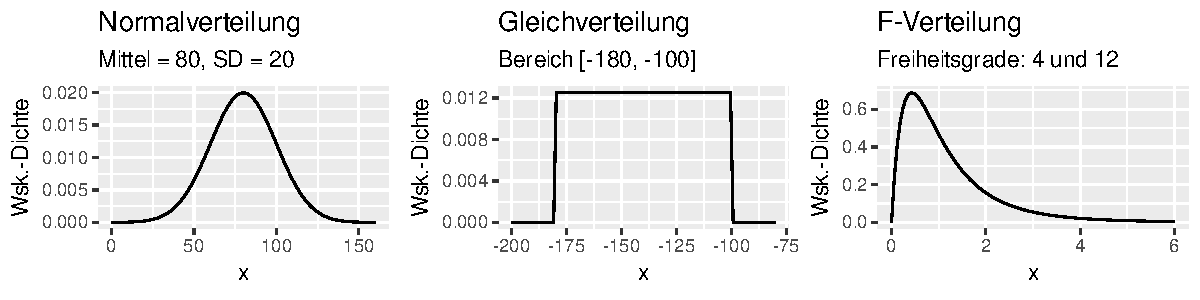
\includegraphics[width=.8\textwidth]{figs/unnamed-chunk-136-1} 

}

\caption{Drei Populationen, aus denen hier Stichproben generiert werden.\label{fig:parentpopulation}}\label{fig:unnamed-chunk-136}
\end{figure}

\end{knitrout}


\paragraph{Aufgabe 2: Stichproben aus einer Gleichverteilung.}
Für die zweite Aufgabe ziehen wir Stichproben aus einer
Gleichverteilung mit Bereich [-180, -100]. Diese Verteilung
hat $\mu = -140$ und $\sigma^2 \approx 533$.

\begin{enumerate}
\item Übernehmen Sie den Code auf Seite \pageref{code:stichprobenmittel}
und passen Sie ihn so an, dass er Stichproben aus dieser
Gleichverteilung generiert.

\item Verwenden Sie diesen Code, um 1'000 Stichproben mit je
2 Beobachtungen aus dieser Verteilung zu generieren und ihr Mittel
zu berechnen.

\item Zeichnen Sie ein Histogramm der 1'000 Stichprobenmittel.
Beschreiben Sie die Verteilung der Stichprobenmittel.
Achten Sie dabei auch auf die Werte auf der $x$-Achse.

\item Berechnen Sie die Varianz der 1'000 Stichprobenmittel und notieren
Sie das Ergebnis.

\item Wiederholen Sie Schritte 2--4 für Stichproben mit
5, 20 und 100 Beobachtungen. Was stellen Sie fest?
\end{enumerate}


\paragraph{Aufgabe 3: Stichproben aus einer schiefen Verteilung.}
Für die dritte Aufgabe ziehen wir Stichproben aus einer
rechtsschiefen Verteilung. Es handelt sich hier um eine
$F$-Verteilung mit den Freiheitsgraden (= Parametern) 4 und 12.
Was eine $F$-Verteilung ist, ist im Moment nicht wichtig; wichtig
ist nur, dass es sich um eine rechtsschiefe Verteilung handelt.
Die $F(4, 12)$-Verteilung hat
$\mu = 1.2$ und $\sigma^2 = 1.26$.

\begin{enumerate}
\item Übernehmen Sie den Code auf Seite \pageref{code:stichprobenmittel}
und passen Sie ihn so an, dass er Stichproben aus einer $F(4, 12)$-Verteilung
generiert.
Statt des \texttt{runif(n = groesse, min = -5, max = 5)}-Befehls
brauchen Sie \texttt{rf(n = groesse, df1 = 4, df2 = 12)}.

\item Verwenden Sie diesen Code, um 1'000 Stichproben mit je
2 Beobachtungen aus dieser Verteilung zu generieren und ihr Mittel
zu berechnen.

\item Zeichnen Sie ein Histogramm der 1'000 Stichprobenmittel.
Beschreiben Sie die Verteilung der Stichprobenmittel.
Achten Sie dabei auch auf die Werte auf der $x$-Achse.

\item Berechnen Sie die Varianz der 1'000 Stichprobenmittel und notieren
Sie das Ergebnis.

\item Wiederholen Sie Schritte 2--4 für Stichproben mit
5, 20 und 100 Beobachtungen. Was stellen Sie fest?
\end{enumerate}

\subsection{Fazit: Der zentrale Grenzwertsatz}
Die Simulationen oben sollen den \textbf{zentralen Grenzwertzsatz}
(\textit{central limit theorem} (CLT)) illustrieren.\footnote{Es ist übrigens der Satz, der zentral (also von zentraler Bedeutung) ist, nicht der Grenzwert.} Dieser
Satz besagt Folgendes:

Wenn Zufallsstichproben mit $n$ Beobachtungen
aus einer Population
mit Mittel $\mu$ und Varianz $\sigma^2$
gezogen werden,\footnote{Es gibt ein paar Wahrscheinlichkeitsverteilungen,
die kein Mittel oder keine Varianz haben.
Für diese gilt der zentrale Grenzwertsatz nicht.}
sind die Stichprobenmittel
ungefähr normalverteilt, wenn $n$ gross genug ist.
Dies gilt auch dann,
wenn die Population selber nicht normalverteilt ist.
Das Mittel der \textbf{Verteilung der Stichprobenmittel}
($\mu_{\bar{x}}$) ist gleich dem Populationsmittel ($\mu$).
Die Varianz der Stichprobenmittel ($\sigma^2_{\bar{x}}$)
wird kleiner, je grösser die Stichproben sind:
\begin{equation*}
\sigma^2_{\bar{x}} = \frac{\sigma^2}{n}.
\end{equation*}

Die Standardabweichung der Verteilung der Stichprobenmittel,
der \textbf{Standardfehler} (\textit{standard error} (S.E.); $\sigma_{\bar{x}}$),
ist daher
\begin{equation*}
\sigma_{\bar{x}} = \sqrt{\frac{\sigma^2}{n}} = \frac{\sigma}{\sqrt{n}}.
\end{equation*}

Diese Einsichten---dass die Mittel genügend grosser
Stichproben annähernd normalverteilt sind und dass
die Varianz dieser Normalverteilung proportional zur
Stichprobengrösse ab\-nimmt---sind von grösster Bedeutung
für die Inferenzstatistik, wie wir später sehen werden.
Es stellt sich somit die Frage, was mit ``wenn $n$ gross genug ist''
gemeint ist.

Die Antwort auf diese Frage hängt von der Population,
aus der die Stichproben stammen, ab. Die Simulationen
sollen zeigen, dass bei Normalverteilungen
die Stichprobenmittel bereits
bei den kleinsten Stichprobengrössen
normalverteilt sind.
Auch bei \emph{fast} normalverteilten Populationen
und sogar bei gleichverteilten Populationen
ist die Stichprobenmittelverteilung bereits bei
ziemlich kleinen Stichproben annähernd normalverteilt.
Bei schiefen Populationen, dahingegen,
kann die Stichprobenmittelverteilung durchaus
noch ein bisschen Schiefe aufweisen, auch
wenn die Stichprobengrösse respektabel ist.

Impräzise\footnote{Die genaue
mathematische Formulierung des zentralen Grenzwertsatzes
lässt an Präzision natürlich nichts zu wünschen übrig.} 
an diesem Satz mag ausserdem erscheinen,
dass er besagt,
dass die Stichprobenmittel \emph{annähernd}
normalverteilt sein werden. Normalverteilungen
reichen eigentlich von $-\infty$ bis $\infty$.
Wenn man aber Stichproben aus, zum Beispiel,
einer Gleichverteilung mit Bereich [-5, 20]
generiert, dann werden die Stichprobenmittel
natürlich immer zwischen -5 und 20 liegen.
In diesem Sinne könnte die Verteilung der
Stichprobenmittel aus dieser Population nie
perfekt normalverteilt sein. Aber auch mit
annähernd normalverteilten Stichprobenmitteln
kommt man ein Stück weiter.

\paragraph{Beispiel 1.}
Die Verteilung der Mittel von Stichproben
mit Grösse 36 aus einer Normalverteilung
mit $\mu = 1.2$ und $\sigma^2 = 4.1$ hat
ein Mittel von 1.2 und eine Standardabweichung
von $\sqrt{\frac{4.1}{36}} \approx 0.34$ (= Standardfehler).
Mit Stichprobengrössen von 50 bzw.\ 100
wäre der Standardfehler
$\sqrt{\frac{4.1}{50}} \approx 0.29$
bzw.\
$\sqrt{\frac{4.1}{100}} \approx 0.20$.
Wer Lust hat, kann dies mit einer Simulation überprüfen.

\paragraph{Beispiel 2.}
Wenn man mit einem fairen 6-seitigen Würfel
würfelt sind die Werte 1, 2, 3, 4, 5 und 6
alle gleich wahrscheinlich. Anders als bei
der kontinuierlichen Gleichverteilung
aus Abschnitt \ref{sec:continuousuniform}
kann aber nicht jeder Wert im Bereich beobachtet
werden: Man kann ja keine 1.72 würfeln.
Eine solche Verteilung nennt man eine
\textbf{diskrete Gleichverteilung}.

Der zentrale Grenzwertsatz trifft auch auf
diskrete Gleichverteilungen zu. In diesem
Fall hat die diskrete Gleichverteilung ein
Mittel von 3.5 und eine Standardabweichung
von 1.71 (oder eine Varianz von 2.92).
Wenn man also mit 10 Würfeln mehrmals würfelt
und jeweils das Mittel der Augen notiert,
wird man feststellen, dass die Mittel
ungefähr normalverteilt sind mit $\mu_{\bar{x}} = \mu = 3.5$
und $\sigma_{\bar{x}} = \frac{1.71}{\sqrt{10}} = 0.54$.
Würfelt man mit 25 Würfeln, dann beträgt
der Standardfehler $\frac{1.71}{\sqrt{25}} = 0.34$.

Überprüfen wir dies doch einmal mit einer kleinen Simulation:
\begin{knitrout}
\definecolor{shadecolor}{rgb}{0.969, 0.969, 0.969}\color{fgcolor}\begin{kframe}
\begin{alltt}
\hlstd{> }\hlstd{wuerfel} \hlkwb{<-} \hlnum{1}\hlopt{:}\hlnum{6}
\hlstd{> }\hlstd{n_sample} \hlkwb{<-} \hlnum{10}
\hlstd{> }\hlstd{n_sim} \hlkwb{<-} \hlnum{10000}
\hlstd{> }\hlstd{mittel} \hlkwb{<-} \hlkwd{vector}\hlstd{(}\hlkwc{length} \hlstd{= n_sim)}
\hlstd{> }\hlkwa{for} \hlstd{(i} \hlkwa{in} \hlnum{1}\hlopt{:}\hlstd{n_sim) \{}
\hlstd{+ }  \hlstd{wuerfe} \hlkwb{<-} \hlkwd{sample}\hlstd{(}\hlkwc{x} \hlstd{= wuerfel,} \hlkwc{size} \hlstd{= n_sample,} \hlkwc{replace} \hlstd{=} \hlnum{TRUE}\hlstd{)}
\hlstd{+ }  \hlstd{mittel[[i]]} \hlkwb{<-} \hlkwd{mean}\hlstd{(wuerfe)}
\hlstd{+ }\hlstd{\}}
\hlstd{> }\hlkwd{sd}\hlstd{(mittel)} \hlcom{# Standardfehler für n = 10}
\end{alltt}
\begin{verbatim}
[1] 0.5376
\end{verbatim}
\end{kframe}
\end{knitrout}


\section{Aufgaben}
\begin{enumerate}
\item Sie möchten wissen, wie viele Bücher im Schnitt
in Schweizer Wohnzimmern vorhanden sind. Nach dem Zufallsprinzip
wählen Sie acht Haushalte aus. Im Wohnzimmer jedes Haushalts zählen
Sie die Anzahl Bücher pro Haushalt. Dies sind Ihre Ergebnisse:
\[
  18, 10, 7, 142, 48, 27, 257, 14.
\]
Tragen Sie diese Daten wie folgt in R ein:
\begin{knitrout}
\definecolor{shadecolor}{rgb}{0.969, 0.969, 0.969}\color{fgcolor}\begin{kframe}
\begin{alltt}
\hlstd{> }\hlstd{buecher} \hlkwb{<-} \hlkwd{c}\hlstd{(}\hlnum{18}\hlstd{,} \hlnum{10}\hlstd{,} \hlnum{7}\hlstd{,} \hlnum{142}\hlstd{,} \hlnum{48}\hlstd{,} \hlnum{27}\hlstd{,} \hlnum{257}\hlstd{,} \hlnum{14}\hlstd{)}
\end{alltt}
\end{kframe}
\end{knitrout}
Sie können die Daten auch in ein Spreadsheet eintragen und dieses Spreadsheet in R einlesen.
\begin{enumerate}
\item Stellen Sie diese Daten grafisch dar und beschreiben Sie ihre Verteilung.
\item Was ist Ihre beste Schätzung des Mittels der Anzahl Bücher pro Schweizer Haushalt?
\item Was ist Ihre beste Schätzung der Varianz und der Standardabweichung der Anzahl Bücher pro Schweizer Haushalt?
\item Erklären Sie, warum wir es hier mit Schätzungen zu tun haben.
      Warum sind wir uns nicht sicher, was das Mittel und die Streuung der Population betrifft?
\end{enumerate}

\item Eine Gleichverteilung mit Bereich [-0.39, 20.39] hat $\mu = 10$ und $\sigma^2 = 36$.

\begin{enumerate}
\item Wie wahrscheinlich ist es, dass eine Zufallsstichprobe mit 4
Beobachtungen aus dieser Verteilung ein Mittel von 5 oder weniger hat? Sie können davon ausgehen,
dass der zentrale Grenzwertsatz zutrifft.

\item Idem, aber für 10 Beobachtungen und für 50 Beobachtungen.

\item Wie viel Prozent der Stichprobenmittel liegen mehr als
4 Einheiten von $\mu$ entfernt bei $n = 8$?

\item Zwischen welchen zwei Werten liegen, symmetrisch um $\mu$,
66.7\% der Stichprobenmittel bei $n = 10$ und bei $n = 60$?
Wie gross ist diese Entfernung zu $\mu$, wenn man sie in Standardfehlern ausdrückt?

\item Idem, aber für 90\% und 95\% der Stichprobenmittel.
\end{enumerate}
\end{enumerate}

\section{Nicht-zufällige Stichproben}
Wir haben uns in diesem Kapitel mit \textbf{Zufallsstichproben}
(\textit{random samples}) beschäftigt,
also mit Stichproben, bei denen jedes Element in der Population
die gleiche Wahrscheinlichkeit hat, ausgewählt zu werden, und bei
denen die Auswahl eines Elements die Auswahl eines anderen Elementes
nicht beeinflusst.
Zwei grosse Vorteile von Zufallsstichproben sind,
dass sie unverzerrte Schätzungen des Populationsmittels und der
Populationsvarianz liefern und dass der zentrale Grenzwertsatz
auf sie zutrifft.

In der Praxis ist es jedoch schwierig, eine Zufallsstichprobe
aus einer einigermassen interessanten Population zu ziehen.
Wenn wir etwa anhand einer Zufallsstichprobe die Englischkenntnisse
bei Erwachsenen kosovarischer Herkunft im Kanton Sankt-Gallen
charakterisieren möchten, brauchen wir zuerst eine vollständige
Liste aller Erwachsenen kosovarischer Herkunft in SG.
Dann müssten wir zufällig eine Stichprobe von ihnen auswählen
und die Ausgewählten alle von einer Teilnahme an der Studie überzeugen:
Sobald sich eine Person weigert, mitzumachen, hätten wir keine
Zufallsstichprobe aus der ursprünglichen Population mehr.
Stattdessen hätten wir eine Stichprobe aus der Population
der in SG wohnhaften Erwachsenen kosovarischer Herkunft, die
bei einer solchen Studie mitmachen möchten. Unsere Schätzungen
würden sich in erster Linie auf diese neue Population beziehen, nicht
auf die Population, für die wir uns anfangs interessierten.

Das Beispiel macht auch klar, was die Konsequenz hiervon ist:
Während eine Zufallsstichprobe eine unverzerrte Schätzung des
Mittels der Population, die eigentlich von Interesse ist, liefert,
wäre es bei einigen Weigerungen möglich, dass einige der ausgewählten
Personen nicht zur Teilnahme bereit sind, gerade weil sie ihre
Englischkenntnisse als ungenügend einschätzen oder weil sie
sprachwissenschaftliche Forschung für uninteressant halten.
Die Übrigen dürften also tendenziell eher gut im Englischen sein
oder sich eher für Sprachen interessieren.
Das Mittel dieser Stichprobe dürfte entsprechend das
Mittel der Population, die ursprünglich von Interesse war,
eher über- als unterschätzen.

Fazit: Statt Zufallsstichproben werden in den Sozialwissenschaften
meistens nicht-zu\-fäll\-ige Stichproben verwendet. Die Konsequenz
davon ist, dass man sich bei der Interpretation der Ergebnisse
mehr Gedanken machen muss, wenn man Rückschlüsse über eine Population
ziehen möchte, als wenn die Stichprobe zufällig ausgewählt worden wäre.

\begin{itemize}
\item Eine Meinungsumfrage auf Twitter erreicht
tendenziell Menschen ähnlicher Meinung. Aber sogar die angesehensten Meinungs\-forschungs\-institute können keine
Zufallsstichproben organisieren: Bei Telefonumfragen in den USA
nehmen nur \href{http://www.pewresearch.org/2017/05/15/what-low-response-rates-mean-for-telephone-surveys/}{etwa 10\%} der Ausgewählten teil.

\item Wer ohne Entgelt einen langen Fragebogen
zu seinem mehrsprachigen
Verhalten ausfüllt, findet Mehrsprachigkeit tendenziell wichtiger
als jemand, der nach der dritten Frage das Browserfenster schliesst
oder den Fragebogen nicht einmal erhalten hat
(bei einer Erhebung nach dem Schneeballprinzip).

\item Muster in einer gut ausgebildeten Stichprobe
mit überdurchschnittlichem
sozioökonomischem Status (z.B.\ Universitätsstudierende)
dürften nicht auf Populationen mit niedrigerem
Bildungsniveau oder sozioökonomischen Status generalisieren
lassen.
Dies ist natürlich vor allem relevant, wenn
Bildung und der sozioökonomische Status wichtig für
den Forschungsgegenstand sind. Wenn man bereit ist, anzunehmen,
dass diese Faktoren nur einen minimalen Effekt auf die Befunde haben,
kann man zuversichtlicher generalisieren.
Ob eine solche Annahme berechtigt ist,
ist eine sachlogische---keine statistische---Frage.
\end{itemize}


\chapter{Die Unsicherheit von Schätzungen einschätzen}\label{ch:uncertainty}
Eine unumgängliche Gegebenheit beim Arbeiten mit Stichproben
ist, dass wir Eigenschaften von Populationen
(`Populationsparameter', z.B.\ Mittelwerte und Streuungsmasse,
aber auch andere Parameter,
denen wir in den nächsten Kapiteln begegen
werden) nur \emph{schätzen} können. Die Frage stellt sich, wie
genau diese Schätzungen denn sind. Interessanterweise wissen wir
dies in der Regel auch nicht genau, weshalb diese Unsicherheit
\emph{auch} anhand der Stichprobe geschätzt werden muss.

Das Ziel dieses Kapitels ist es, anhand eines Beispiels zu
illustrieren, wie man mit einer Stichprobe die Unsicherheit
in einer Parameterschätzung einschätzen kann.
Dazu introduziert dieses Kapitel den sog.\ \textbf{Bootstrap},
ein flexibles, mechanistisches Verfahren,
um Unsicherheit einzuschätzen.
Danach wird gezeigt, wie man anhand des zentralen Grenzwertsatzes
(Kapitel \ref{ch:stichproben}) das Gleiche machen kann.

Im Folgenden arbeiten wir mit einem Datensatz
aus der Studie von \citet{DeKeyser2010}.
Diese untersuchten, wie das Alter,
in dem MigrantInnen angefangen haben, eine Zweitsprache
zu lernen (\textit{age of acquisition}, AOA),
mit ihrer Leistung bei einer Grammatikaufgabe
zusammenhängt (\textit{grammaticality judgement task}, GJT).
Die Teilnehmenden waren russische MigrantInnen in Israel
und in Nordamerika.
Die Grammatikaufgabe bestand aus 204 richtig/falsch-Items.
In den nächsten Kapiteln werden wir uns mit dem
Zusammenhang zwischen AOA und GJT befassen;
hier verwenden wir den Datensatz von \citet{DeKeyser2010},
um zu zeigen, wie man die Unsicherheit bei Stichprobenschätzungen
quantifizieren kann.



\paragraph{Aufgabe.}
Der Datensatz \texttt{dekeyser2010.csv} enthält
die AOA- und GJT-Daten der russischen MigrantInnen
in Nordamerika.
Lesen Sie diesen Datensatz in R ein.
Zeichnen Sie die Grafik in Abbildung \ref{fig:gjthistogram} selbst.
Berechnen Sie zudem das Mittel der GJT-Werte.

\begin{knitrout}
\definecolor{shadecolor}{rgb}{0.969, 0.969, 0.969}\color{fgcolor}\begin{figure}[tp]

{\centering 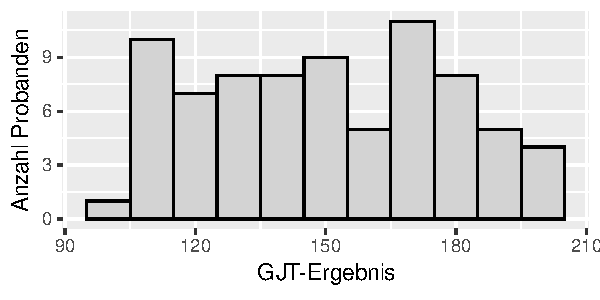
\includegraphics[width=.4\textwidth]{figs/unnamed-chunk-140-1} 

}

\caption{Histogramm der GJT-Daten aus der Nordamerika-Studie von \citet{DeKeyser2010}. Diese Grafik sollten Sie selber zeichnen (Aufgabe 1).\label{fig:gjthistogram}}\label{fig:unnamed-chunk-140}
\end{figure}

\end{knitrout}

\section{Stichprobenmittel variieren}
Lasst uns davon ausgehen,
dass die GJT-Daten in der ganzen
Population genau so verteilt wären wie in
Abbildung \ref{fig:gjthistogram}.
Dies ist nur eine Annahme für didaktische Zwecke.
Als Forschende haben wir keinen Zugriff zur ganzen Population,
d.h., wir wissen eigentlich nicht,
wie dieses Populationsverteilung aussieht.
Stattdessen müssen wir uns mit Stichproben begnügen.
Aber nehmen wir vorübergehend an, dass die Daten in der Population
genau so verteilt wären wie in dieser Stichprobe.

Wie schon in Kapitel \ref{ch:stichproben} besprochen,
bilden die Mittel von Zufallsstichproben mit der gleichen Grösse
eine Stichprobenmittelverteilung, deren Mittel gleich dem
Populationsmittel ist ($\mu_{\bar{x}} = \mu$).
Abbildung \ref{fig:stichprobenauspopulation} zeigt exemplarisch fünf
Stichproben mit Grösse 20 aus dieser GJT-Population und die
Verteilung der Mittel von 20'000 Stichproben mit je 20 Beobachtungen aus
der Population.
Die Standardabweichung der Stichprobenmittelverteilung,
der Standardfehler (siehe Kapitel \ref{ch:stichproben}),
beträgt 6.06 Punkte.
2.5\% der Stichprobenmittel sind kleiner als 138.95;
2.5\% sind grösser als 162.60.
95\% aller Stichprobenmittel liegen also in einem Intervall
von $162.60-138.95 = 23.65$ Punkten.
Der Standardfehler oder die Breite eines solchen Intervalls
wären sinnvolle Masse für die Genauigkeit, mit der man mit einer
Stichprobe einen Populationsparameter schätzen kann.

\begin{knitrout}
\definecolor{shadecolor}{rgb}{0.969, 0.969, 0.969}\color{fgcolor}\begin{figure}[tp]

{\centering 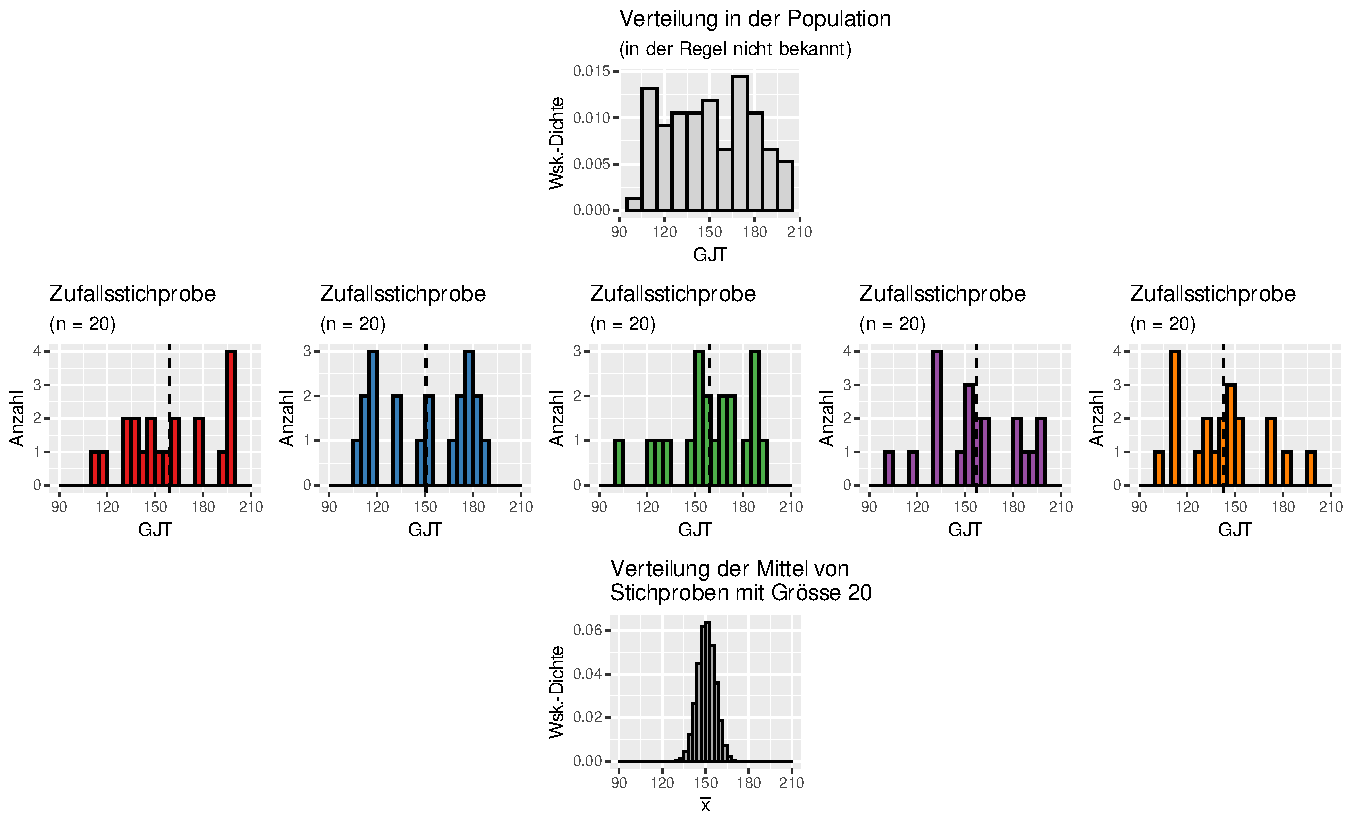
\includegraphics[width=\textwidth]{figs/unnamed-chunk-141-1} 

}

\caption{Wenn eine grosse Anzahl Zufallsstichproben mit der gleichen Grösse aus der Population gezogen werden und je ihr Mittel berechnet wird (senkrechte Linie), ergibt sich die Stichprobenmittelverteilung. In diesem Fall ist diese normalverteilt, aber dies ist nicht unbedingt der Fall. Exemplarisch werden fünf der Stichproben gezeigt.\label{fig:stichprobenauspopulation}}\label{fig:unnamed-chunk-141}
\end{figure}

\end{knitrout}

Unser Problem ist aber, dass wir die Stichprobenmittelverteilung
nur generieren können, wenn wir Zugriff zur ganzen Population haben.
Wenn wir nur über eine Stichprobe verfügen, müssen wir den
Standardfehler bzw.\ die Breite solcher Intervalle anhand der
Stichprobe schätzen.

\section{Das \textit{plug-in}-Prinzip und der \textit{Bootstrap}}
\emph{Enter the plug-in principle.}
Abbildung \ref{fig:stichprobenauspopulation} zeigt zwar,
dass jede einzelne Stichprobe die Population nur imperfekt
widerspiegelt. Aber gleichzeitig ist diese Widerspieglung
das Beste, was wir in der Praxis haben.\footnote{Sogenannte bayessche
Methoden erlauben es einem aber, auch Informationen, die man nicht
aus den Daten selber ableiten kann, in der Analyse zu berücksichtigen.}
Um den Standardfehler bzw.\ die
Form der Stichprobenmittelverteilung zu schätzen, können wir
die Stichprobe als Stellvertreter der Population
betrachten.\footnote{Dieser Abschnitt wurde von \citet{Hesterberg2015} inspiriert.}

\subsection{Zwei Beispiele}

\paragraph{Beispiel 1.}
Abbildung \vref{fig:bootstrap_rot} zeigt das Vorgehen.
Zur Verfügung steht uns die erste (rote) Stichprobe aus Abbildung
\ref{fig:stichprobenauspopulation}. Wir tun nun, als ob die GJT-Population
genau so wie diese Stichprobe verteilt wäre, denn wir haben
keine besseren Anknüpfungspunkte. Um die Stichprobenmittelverteilung
zu generieren, ziehen wir Zufallsstichproben mit Grösse 20
aus dieser Stichprobe.\footnote{Ein Detail: Eine Beobachtung
darf mehrmals in der gleichen Stichprobe vorkommen. Dies nennt
man \textit{sampling with replacement} und man macht es, weil
man davon ausgeht, dass die Population (praktisch gesehen) unendlich gross ist.}
Diese Stichproben werden
\textit{Bootstrap}-Stichproben (oder \textit{bootstrap replicates})
genannt. Abbildung \ref{fig:bootstrap_rot} zeigt exemplarisch
drei solche \textit{Bootstrap}-Stichproben.
Für jede Bootstrap-Stichprobe können wir das Mittel berechnen;
die Verteilung von 20'000 dieser Mittel steht in der unteren Grafik.

\begin{knitrout}
\definecolor{shadecolor}{rgb}{0.969, 0.969, 0.969}\color{fgcolor}\begin{figure}[tp]

{\centering 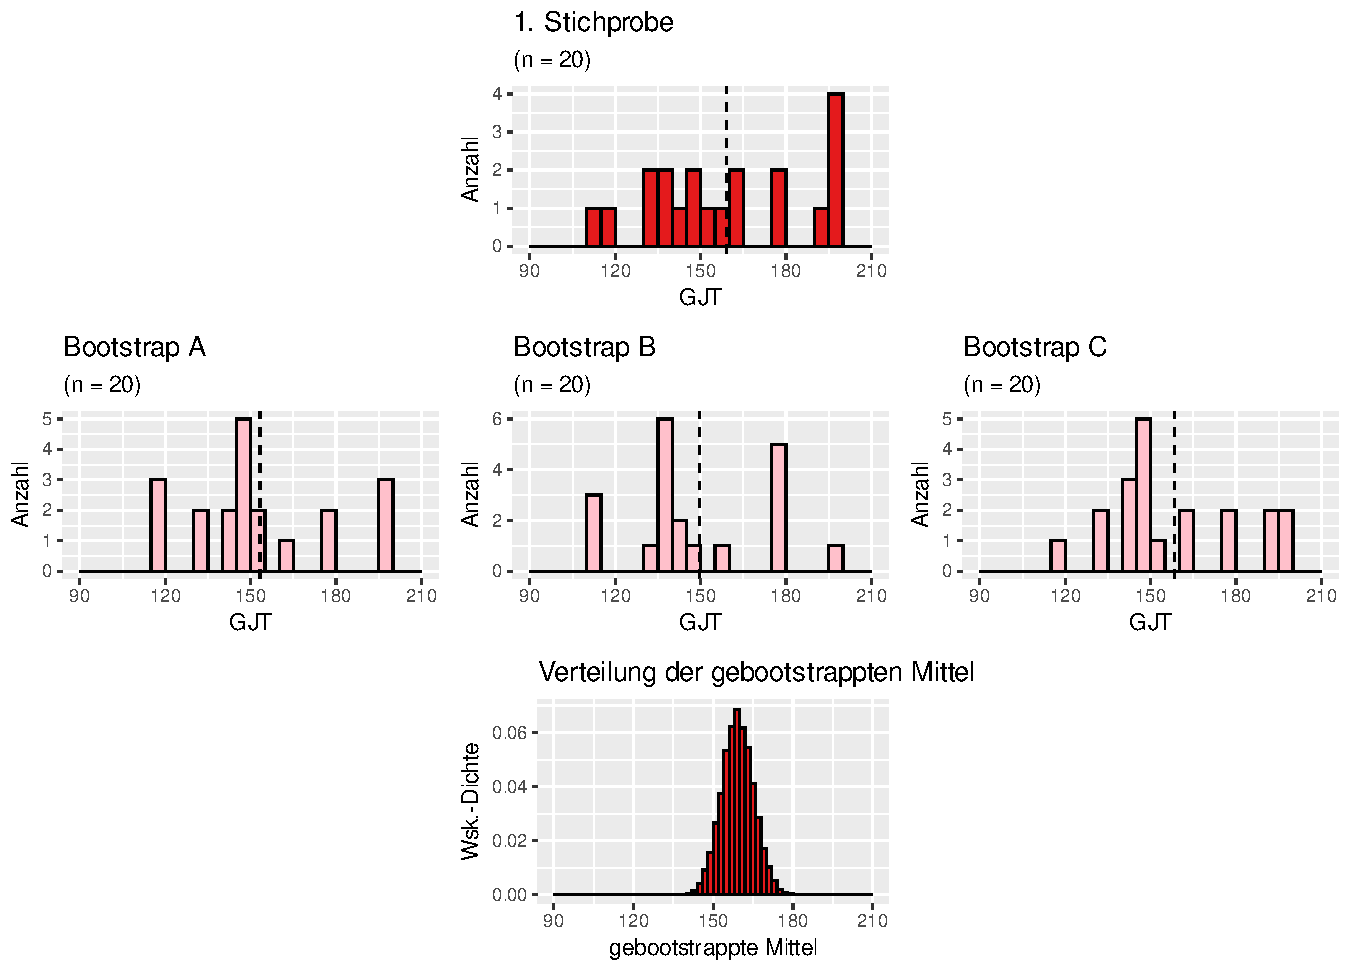
\includegraphics[width=\textwidth]{figs/unnamed-chunk-142-1} 

}

\caption{Die erste Stichprobe aus Abbildung \ref{fig:stichprobenauspopulation} dient hier als Stellvertreter der GJT-Population. Exemplarisch werden drei Bootstrap-Stichproben mit Grösse 20 gezeigt. Wenn man 20'000 solche Bootstrap-Stichproben generiert, bilden ihre Mittel die Verteilung in der unteren Grafik. Diese hier schaut normalverteilt aus, aber dies ist nicht zwingend der Fall.\label{fig:bootstrap_rot}}\label{fig:unnamed-chunk-142}
\end{figure}

\end{knitrout}

Das Mittel der gebootstrappten Mittel ist gleich dem Mittel
der Stichprobe (145.95).
Ihre Standardabweichung beträgt etwa 5.20.
2.5\% der gebootstrappten Mittel sind kleiner als 135.95;
2.5\% sind grösser als 156.20;
die Breite dieses Intervalls ist also 20.25 Punkte.

\paragraph{Beispiel 2.}
Abbildung \vref{fig:bootstrap_blau} zeigt das Verfahren noch einmal,
diesmal mit der zweiten (blauen) Stichprobe aus Abbildung
\ref{fig:stichprobenauspopulation} als Ausgangspunkt.
Das Mittel der gebootstrappten Mittel ist gleich dem Mittel
der Stichprobe (146.85).
Ihre Standardabweichung beträgt etwa 7.03.
2.5\% der gebootstrappten Mittel sind kleiner als 133.55;
2.5\% sind grösser als 161.00;
die Breite dieses Intervalls ist also 27.45 Punkte.

\begin{knitrout}
\definecolor{shadecolor}{rgb}{0.969, 0.969, 0.969}\color{fgcolor}\begin{figure}[tp]

{\centering 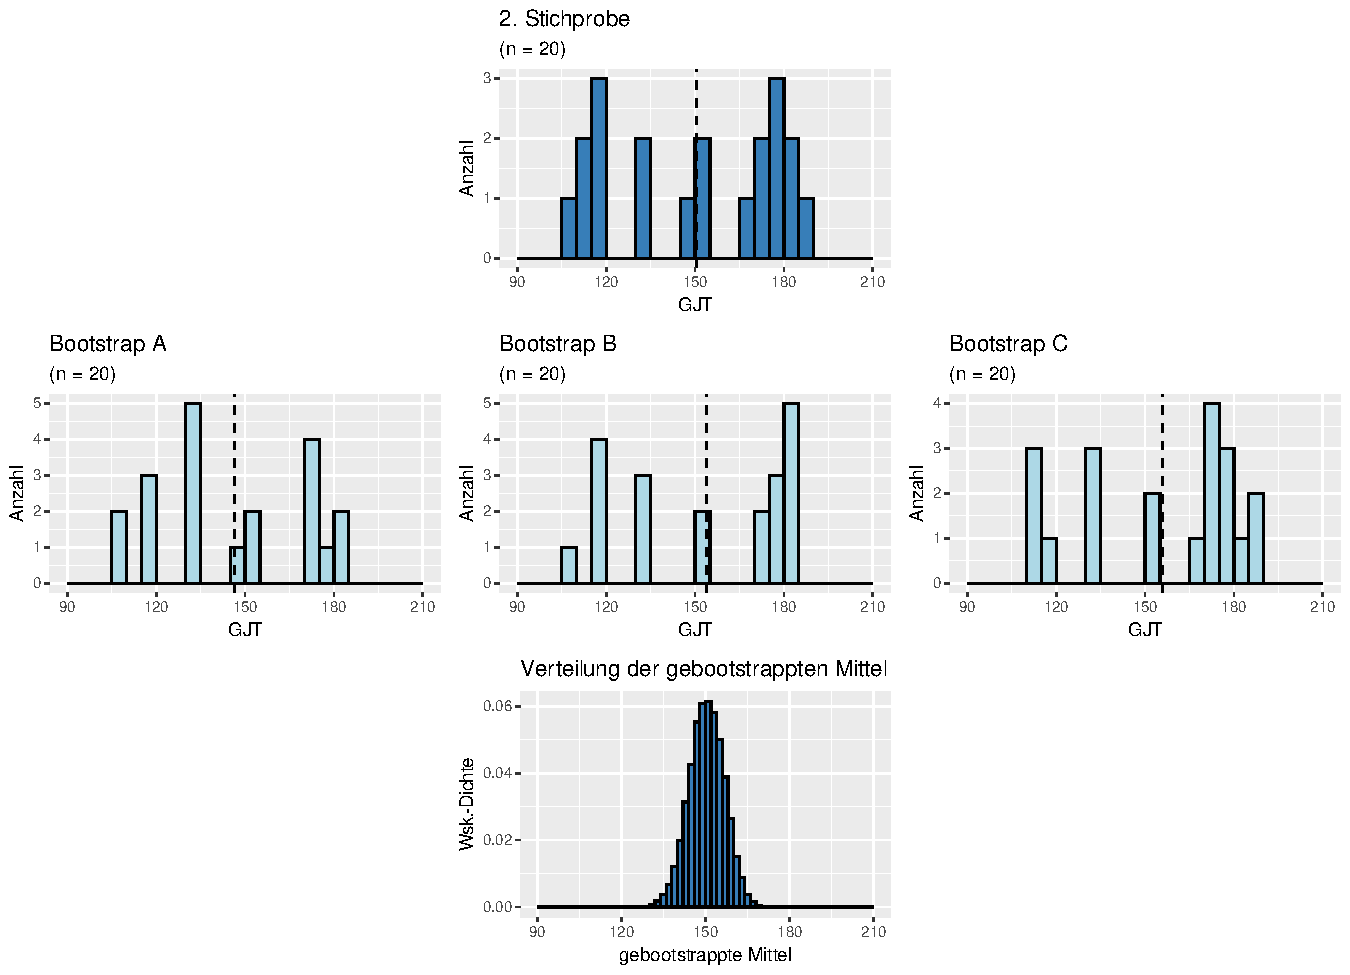
\includegraphics[width=\textwidth]{figs/unnamed-chunk-143-1} 

}

\caption{Die zweite Stichprobe aus Abbildung \ref{fig:stichprobenauspopulation} dient hier als Stellvertreter der GJT-Population. Exemplarisch werden drei Bootstrap-Stichproben mit Grösse 20 gezeigt. Wenn man 20'000 solche Bootstrap-Stichproben generiert, bilden ihre Mittel die Verteilung in der unteren Grafik. Diese hier schaut normalverteilt aus, aber dies ist nicht zwingend der Fall.\label{fig:bootstrap_blau}}\label{fig:unnamed-chunk-143}
\end{figure}

\end{knitrout}

\subsection{Die Essenz des Bootstraps}
Der Bootstrap ist eine Technik,
um die Unsicherheit in Parameterschätzungen
zu quantifizieren \citep{Efron1979,Efron1993}. Die tatsächliche Unsicherheit in einer Parameterschätzung
können wir nur berechnen, wenn wir eine grosse Anzahl Stichproben aus der gleichen
Population ziehen und feststellen, wie die Schätzungen zwischen den Stichproben
variieren:
\begin{itemize}
\item Population definieren,\\
$\rightarrow$ Stichproben ziehen,\\
$\rightarrow$ Verteilung von Schätzungen in Stichproben generieren,\\
$\rightarrow$ Variabilität in Schätzung berechnen.
\end{itemize}

Mangels einer grossen Anzahl Stichproben aus der gleichen Population,
verlässt man sich auf das \textit{plug-in}-Prinzip: Die Stichprobe
tritt stellvertretend für die Population auf, und geschaut wird,
wie gut Stichproben einer bestimmten Grösse aus dieser Stichprobe
den untersuchten Parameter schätzen können.
\begin{itemize}
\item Stichprobe definieren, \\
$\rightarrow$ Bootstrap-Stichproben ziehen, \\
$\rightarrow$ Verteilung von Schätzungen in Bootstrap-Stichproben generieren, \\
$\rightarrow$ Variabilität in Schätzung. \emph{schätzen}
\end{itemize}

Der Bootstrap ergibt eine \emph{Schätzung}
der Unsicherheit in der Parameterschätzung.
Das wird klar, wenn man sich Abbildung
\vref{fig:bootstrapdistributions}
und Tabelle \ref{tab:bootstrap} anschaut.
Abbildung \ref{fig:bootstrapdistributions} zeigt die
Verteilung der gebootstrappten Mittel für die fünf Stichproben;
Tabelle \ref{tab:bootstrap} fasst ihre Standardabweichung,
ihre 2.5. und 97.5. Perzentile, und den Unterschied zwischen
diesen Perzentilen zusammen.
Die Standardabweichungen und die Breite der Intervalle
zwischen dem 2.5.\ und dem 97.5.\ Perzentil sind in keinem
der fünf Beispiele dem entsprechenden
tatsächlichen, aber unbekannten Wert, gleich.
Aber im Schnitt sind sie ihm recht ähnlich.
Insbesondere wenn man über keine weiteren Anknüpfungspunkte
verfügt
(z.B.\ vorherige Studien, sachlogische Überlegungen),
kann der Bootstrap also nützliche, wenn auch imperfekte,
Informationen über
die Unsicherheit einer Parameterschätzung liefern.

\begin{knitrout}
\definecolor{shadecolor}{rgb}{0.969, 0.969, 0.969}\color{fgcolor}\begin{figure}[tp]

{\centering 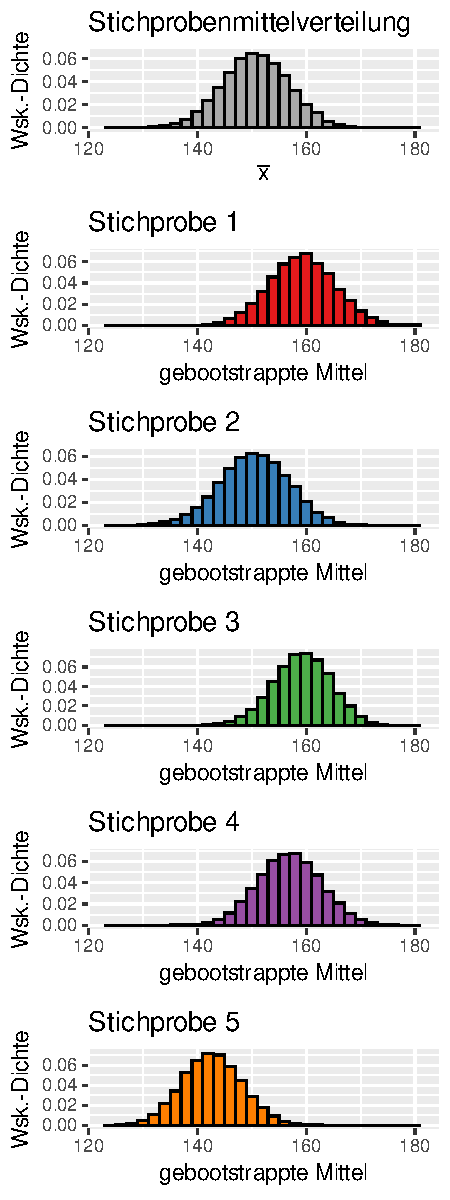
\includegraphics[width=.5\textwidth]{figs/unnamed-chunk-144-1} 

}

\caption{Die Verteilung der gebootstrappten Mittel auf der Basis von fünf Stichproben.\label{fig:bootstrapdistributions}}\label{fig:unnamed-chunk-144}
\end{figure}

\end{knitrout}

\begin{table}[tbp]
\centering
\caption{Standardabweichung, Perzentile und der Unterschied zwischen den Perzentilen für die eigentliche Stichprobenmittelverteilung
und die fünf Verteilungen der gebootstrappten Mittel. Die Perzentile und der Unterschied zwischen ihnen wurden gerundet.}
\label{tab:bootstrap}
\begin{tabular}{lrrrr}
\toprule
Stichprobenmittelverteilung     & $SD$  & 2.5. Perzentil  & 97.5. Perzentil & Unterschied \\
\midrule
Tatsächlich (unbekannt)         & 6.1   & 139          & 163          & 24 \\
\midrule
Bootstrap Stichprobe 1          & 5.2   & 136          & 156          & 20 \\
Bootstrap Stichprobe 2          & 7.0   & 134          & 161          & 27 \\
Bootstrap Stichprobe 3          & 6.0   & 134          & 158          & 23 \\
Bootstrap Stichprobe 4          & 6.9   & 145          & 172          & 27 \\
Bootstrap Stichprobe 5          & 5.9   & 129          & 152          & 23 \\
 \bottomrule
\end{tabular}
\end{table}

\subsection{Vorteile des Bootstraps}

\begin{itemize}
 \item \textbf{Didaktisch wertvoll} (hoffe ich).
 Die mathematischen Anforderungen sind beim Bootstrappen gering.
 Dies erlaubt uns, wichtige Konzepte unabhängig von ihrer üblichen
 mathematischen Umsetzung zu besprechen.

 \item \textbf{Flexibilität.} Hier haben wir uns mit der Unsicherheit eines
 Stichprobenmittels befasst. Diese kann man auch mit einer relativ
 einfachen analytischen Methode ausdrücken (siehe unten). Den Bootstrap
 kann man aber auch verwenden, um die Unsicherheit vieler anderer
 Schätzungen auszudrücken, zum Beispiel eines getrimmten
 oder winsorisierten Mittels, eines Medians,
 einer Standardabweichung, eines bestimmten
 Perzentils, oder irgendwelcher anderen Masse.
 Ausserdem kann der Bootstrap auch bei komplexeren Modellen
 (z.B., wenn wir den Zusammenhang zwischen verschiedenen Variablen untersuchen)
 verwendet werden.

 \item \textbf{Minimale Annahmen.} Verglichen mit anderen Verfahren basiert
 der Bootstrap auf nur wenigen Annahmen. Dieser Punkt wird später
 in diesem Kapitel deutlicher werden,
 aber hier sei bereits darauf
 hingewiesen, dass wir in den
 obigen Beispielen nirgends davon ausgegangen
 sind, dass die Stichprobenmittelverteilung normalverteilt ist.
 In den Beispielen sind die
 Verteilungen der gebootstrappten Mittel zwar
 normalverteilt, aber hiervon sind wir nicht a priori \emph{ausgegangen}.
 Wir sind auch nicht davon ausgegangen,
 dass die Population, aus der
 die Stichproben stammen, normalverteilt ist.
\end{itemize}


\subsection{Nachteile des Bootstraps}

\begin{itemize}
 \item ``Bootstrapping does not overcome the \textbf{weakness of small samples} as a basis for inference.'' \citep[][S.~379]{Hesterberg2015}
 Einerseits ist die \emph{tatsächliche} Unsicherheit einer Parameterschätzung
 bei einer kleinen Stichprobe natürlich grösser als bei einer grösseren (siehe auch
 den zentralen Grenzwertsatz). Aber andererseits ist unsere \emph{Schätzung} dieser
 Unsicherheit bei kleineren Stichproben auch weniger genau als bei grösseren.
 Dies ist aber nicht sosehr ein Nachteil des Bootstraps, sondern von kleinen
 Stichproben im Allgemeinen: Andere Verfahren bieten hier keine bessere Lösung.\footnote{Ausser sie machen striktere Annahmen oder sie berücksichtigen Informationen, die man nicht aus den Daten selber ableiten kann.}

 \item Die Implementierung des Bootstraps, die oben illustriert wurde, tendiert dazu,
 die Unsicherheit einer Parameterschätzung eher zu unter- als zu überschätzen.
 Dies ist umso mehr der Fall bei kleinen Stichproben.
 Der Grund dafür ist, dass eine Stichprobe die Streuung in der Population eher
 unter- als überschätzt; deswegen wird die Varianz einer Stichprobe ja leicht
 anders berechnet als jene einer Population (siehe Abschnitt \vref{sec:stichprobenvarianz}).
 Beim Bootstrap tritt die Stichprobe aber stellvertretend für die Population auf.
 Insofern die Stichprobe die Streuung in der Population unterschätzt, unterschätzt
 der Bootstrap die Unsicherheit der Parameterschätzung.
 Es gibt ein paar Möglichkeiten, diese Verzerrung zu korrigieren
 \citep[siehe][]{Efron1993}, aber pädagogisch
 sind diese hier nicht so interessant.

 \item Da der Bootstrap so flexibel ist, ist es schwierig, eine allgemeine,
 benutzerfreundliche Funktion für ihn zu schreiben.
 Daher muss man den Bootstrap meistens selber programmieren.
\end{itemize}

\subsection{Übungen}
Die obigen Beispiele dienten nur einem pädagogischen Zweck:
Wenn wir eine Stichprobe von 76 Versuchspersonen haben,
ist es ja kaum sinnvoll, kleinere Stichproben aus ihr zu ziehen.
Stattdessen werden hier zuerst die Befehle gezeigt,
mit denen Sie die Unsicherheit von DeKeyser et al.'s
ursprünglichem Stichprobenmittel schätzen können.
Übrigens befinden wir uns dabei in der komischen aber üblichen
Situation, dass wir nicht wirklich wissen, über welche
Population wir genau Aussagen treffen können.
Dann folgen zwei Übungen, die die Flexibilität des Bootstrap
illustrieren.

\paragraph{Übung 1: Mittel.}
Der erste Codeabschnitt definiert, wie
viele bootstrap replicates generiert werden
sollen, generiert diese dann anhand
eines \textit{for-loops} und berechnet
jeweils das Mittel.
In diesem Codeabschnitt wird davon ausgegangen,
dass Sie den Datensatz \texttt{d} genannt haben.
Wenn dies nicht der Fall ist, müssen Sie
überall noch \texttt{d} durch den richtigen
Objektnamen ersetzen oder eben den Datensatz umbenennen.
\begin{knitrout}
\definecolor{shadecolor}{rgb}{0.969, 0.969, 0.969}\color{fgcolor}\begin{kframe}
\begin{alltt}
\hlstd{> }\hlcom{# Anzahl bootstrap replicates}
\hlstd{> }\hlstd{n_bootstraps} \hlkwb{<-} \hlnum{20000}
\hlstd{> }\hlstd{bootstraps} \hlkwb{<-} \hlkwd{vector}\hlstd{(}\hlkwc{length} \hlstd{= n_bootstraps)}
\hlstd{> }
\hlstd{> }\hlkwa{for} \hlstd{(i} \hlkwa{in} \hlnum{1}\hlopt{:}\hlstd{n_bootstraps) \{}
\hlstd{+ }  \hlcom{# Sampling with replacement, daher 'replace = TRUE'.}
\hlstd{+ }  \hlstd{bootstrap_sample} \hlkwb{<-} \hlstd{d |>}
\hlstd{+ }    \hlkwd{slice_sample}\hlstd{(}\hlkwc{prop} \hlstd{=} \hlnum{1}\hlstd{,} \hlkwc{replace} \hlstd{=} \hlnum{TRUE}\hlstd{)}

\hlstd{+ }  \hlcom{# Mittel des bootstrap replicates berechnen und speichern.}
\hlstd{+ }  \hlstd{bootstraps[[i]]} \hlkwb{<-} \hlkwd{mean}\hlstd{(bootstrap_sample}\hlopt{$}\hlstd{GJT)}
\hlstd{+ }\hlstd{\}}
\end{alltt}
\end{kframe}
\end{knitrout}

Hesterberg (2015) empfiehlt, 20'000 bootstrap replicates zu
generieren, sodass das Ergebnis nur minimal vom Zufallsfaktor
im Bootstrap selber beeinflusst wird. Um eine grobe Idee zu
erhalten, würden 1'000 replicates reichen, aber im Prinzip
sollte diese Berechnung nicht sehr lange dauern.
Ein schnelles Histogramm (ohne \texttt{ggplot2}) zeigt
die Wirkung des zentralen Grenzwertsatzes.
\begin{knitrout}
\definecolor{shadecolor}{rgb}{0.969, 0.969, 0.969}\color{fgcolor}\begin{kframe}
\begin{alltt}
\hlstd{> }\hlkwd{hist}\hlstd{(bootstraps)}
\end{alltt}
\end{kframe}
\end{knitrout}

Als Schätzung des Standardfehlers dient
die Standardabweichung der gebootstrappten Mittel.
\begin{knitrout}
\definecolor{shadecolor}{rgb}{0.969, 0.969, 0.969}\color{fgcolor}\begin{kframe}
\begin{alltt}
\hlstd{> }\hlcom{# Standardfehler des Mittels schätzen.}
\hlstd{> }\hlkwd{sd}\hlstd{(bootstraps)}
\end{alltt}
\begin{verbatim}
[1] 3.1352
\end{verbatim}
\end{kframe}
\end{knitrout}

Berichten würde ich die Schätzung des Mittels und die Unsicherheit über diese Schätzung als $150.8 \pm 3.1$ oder sogar als $151 \pm 3$.
$150.7763 \pm 3.1352$ wären aber zu viele Zahlen, über
die es zu viel Unsicherheit gibt. In \citet{Vanhove2020b} habe ich versucht, ein paar
Richtschnuren fürs Abrunden von Schätzungen zu formulieren.

Etwa 95\% der gebootstrappten Mittel liegen
zwischen 145 und 157. Dieses Intervall nennt
man übrigens ein \textbf{Konfidenzintervall},
aber darüber später mehr.
\begin{knitrout}
\definecolor{shadecolor}{rgb}{0.969, 0.969, 0.969}\color{fgcolor}\begin{kframe}
\begin{alltt}
\hlstd{> }\hlkwd{quantile}\hlstd{(bootstraps,} \hlkwc{probs} \hlstd{=} \hlkwd{c}\hlstd{(}\hlnum{0.025}\hlstd{,} \hlnum{0.975}\hlstd{))}
\end{alltt}
\begin{verbatim}
  2.5%  97.5% 
144.54 156.90 
\end{verbatim}
\end{kframe}
\end{knitrout}

Da die Verteilung der gebootstrappten Mittel in etwa
normalverteilt aussieht, können wir diese Perzentile
auch mithilfe der Eigenschaften von Normalverteilungen
berechnen. Das 2.5.\ Perzentil jeder Normalverteilung
liegt etwa 1.96 Standardabweichungen unter dem Mittel:
\begin{knitrout}
\definecolor{shadecolor}{rgb}{0.969, 0.969, 0.969}\color{fgcolor}\begin{kframe}
\begin{alltt}
\hlstd{> }\hlkwd{qnorm}\hlstd{(}\hlnum{0.025}\hlstd{)}
\end{alltt}
\begin{verbatim}
[1] -1.96
\end{verbatim}
\end{kframe}
\end{knitrout}
Und das 97.5.\ Perzentil liegt genauso weit über dem Mittel:
\begin{knitrout}
\definecolor{shadecolor}{rgb}{0.969, 0.969, 0.969}\color{fgcolor}\begin{kframe}
\begin{alltt}
\hlstd{> }\hlkwd{qnorm}\hlstd{(}\hlnum{0.975}\hlstd{)}
\end{alltt}
\begin{verbatim}
[1] 1.96
\end{verbatim}
\end{kframe}
\end{knitrout}
Diese Berechnungsmethode ergibt daher grundsätzlich die gleiche Lösung:
\begin{knitrout}
\definecolor{shadecolor}{rgb}{0.969, 0.969, 0.969}\color{fgcolor}\begin{kframe}
\begin{alltt}
\hlstd{> }\hlkwd{mean}\hlstd{(d}\hlopt{$}\hlstd{GJT)} \hlopt{+} \hlkwd{c}\hlstd{(}\hlopt{-}\hlnum{1.96}\hlstd{,} \hlnum{1.96}\hlstd{)} \hlopt{*} \hlkwd{sd}\hlstd{(bootstraps)}
\end{alltt}
\begin{verbatim}
[1] 144.63 156.92
\end{verbatim}
\end{kframe}
\end{knitrout}
Dies gilt natürlich nur, wenn die Verteilung der gebootstrappten
Mittel normalverteilt ist; die Perzentilmethode ist allgemeiner
gültig.

Verglichen mit den Angaben in Tabelle \ref{tab:bootstrap}
sind der geschätzte Standardfehler und die Breite des Intervalls
kleiner. Können Sie sich erklären, wieso?

\paragraph{Übung 2: getrimmtes Mittel.}\label{par:trimmed}
In Kapitel \ref{ch:descriptives} haben
wir auch das getrimte Mittel kennengelernt.
Wenn wir auf beiden Seiten 20\% der Beobachtungen wegschneiden,
beträgt das Mittel der GJT-Daten etwa 150.7 Punkte:
\begin{knitrout}
\definecolor{shadecolor}{rgb}{0.969, 0.969, 0.969}\color{fgcolor}\begin{kframe}
\begin{alltt}
\hlstd{> }\hlkwd{mean}\hlstd{(d}\hlopt{$}\hlstd{GJT,} \hlkwc{trim} \hlstd{=} \hlnum{0.2}\hlstd{)}
\end{alltt}
\begin{verbatim}
[1] 150.67
\end{verbatim}
\end{kframe}
\end{knitrout}
Schätzen Sie den Standardfehler dieses getrimmten Mittels
mithilfe des Bootstraps.

Hinweis: Sie brauchen lediglich eine Zeile des Codeabschnitts
von Übung 1 leicht anzupassen.

\paragraph{Übung 3: Standardabweichung.}
Der Bootstrap ist nicht nur nützlich, um die Unsicherheit
in der Schätzung eines Mittels zu quantifizieren.
Berechnen Sie die Standardabweichung der GJT-Daten
und verwenden Sie den Bootstrap, um die Unsicherheit in dieser
Schätzung zu quantifizieren.

\paragraph{Übung 4: Median.}
Wie Übung 3, aber mit dem Median statt der Standardabweichung.
Was fällt Ihnen verglichen mit den vorigen Übungen auf? 
Wenn Ihnen nichts auffällt, sollten Sie
die Anzahl \textit{bins} im Histogramm vergrössern: 
\texttt{hist(bootstraps, breaks = 100)}. 
Wie erklären Sie sich Ihren Befund?

\section{Das \textit{plug-in}-Prinzip und der zentrale Grenzwertsatz}
In der Praxis wird der Bootstrap eher selten verwendet, 
um die Unsicherheit eines
Stichprobenmittel zu quantifizieren. Stattdessen verlässt
man sich meistens auf den zentralen Grenzwertsatz (siehe
Abschnitt \vref{sec:clt}).
Zur Erinnerung: Der zentrale Grenzwertsatz besagt, dass
die Verteilung der
Stichprobenmittel ($\bar{x}$) zu einer Normalverteilung neigt,
wenn die Stichproben gross genug sind. Das Mittel
der Stichprobenmittelverteilung ist gleich dem Populationsmittel
($\mu_{\bar{x}} = \mu$); ihre Standardabweichung (der Standardfehler)
beträgt:
\begin{equation*}
\textrm{SE} = \sigma_{\bar{x}} = \frac{\sigma}{\sqrt{n}}.
\end{equation*}
Wenn wir annehmen wollen, dass der zentrale Grenzwertsatz
bereits bei unserer Stichprobengrösse greift, und wir
die Standardabweichung der Population, aus der unsere Stichprobe
stammt, kennen, können wir den Standardfehler also direkt berechnen.
Wenn uns die Standardabweichung der Population nicht bekannt ist,
können wir wieder das \textit{plug-in}-Prinzip anwenden:
Die Stichprobenstandardabweichung $s$ ist die beste Schätzung der
Populationsstandardabweichung $\sigma$, die wir haben, weshalb wir diese
Schätzung stellvertretend in die Formel eintragen:
\begin{equation*}
\textrm{SE} \approx \widehat{\textrm{SE}} = \frac{s}{\sqrt{n}}.
\end{equation*}

Bei den GJT-Daten beträgt die Stichprobenstandardabweichung
etwa 27.23. Daher beträgt der geschätzte Standardfehler
$\frac{27.32}{\sqrt{76}} = 3.13$. Dies ist nahezu die gleiche
Antwort, die wir mit dem Bootstrap bekamen (3.12), was
natürlich beruhigend ist.

Anhand des zentralen Grenzwertsatzes können wir auch ein
95\%-Konfidenzintervall konstruieren:
\begin{knitrout}
\definecolor{shadecolor}{rgb}{0.969, 0.969, 0.969}\color{fgcolor}\begin{kframe}
\begin{alltt}
\hlstd{> }\hlkwd{mean}\hlstd{(d}\hlopt{$}\hlstd{GJT)} \hlopt{+} \hlkwd{c}\hlstd{(}\hlopt{-}\hlnum{1.96}\hlstd{,} \hlnum{1.96}\hlstd{)} \hlopt{*} \hlkwd{sd}\hlstd{(d}\hlopt{$}\hlstd{GJT)}\hlopt{/}\hlkwd{sqrt}\hlstd{(}\hlnum{76}\hlstd{)}
\end{alltt}
\begin{verbatim}
[1] 144.63 156.92
\end{verbatim}
\end{kframe}
\end{knitrout}

Auch das Konfidenzintervall ist dem Konfidenzintervall,
das mit dem Bootstrap konstruiert wurde, sehr ähnlich.

Bemerken Sie aber, dass wir diesmal
davon \emph{ausgegangen} sind, dass die Stichprobenmittel aus
der Population normalverteilt sind; diese Annahme haben
wir beim Bootstrap nicht gemacht. Bei sehr schiefen oder
anderen asymmetrischen Verteilungen ist es durchaus möglich,
dass der zentrale Grenzwertsatz auch bei Stichproben von 76
Beobachtungen noch nicht greift. Wenn dieser Verdacht besteht,
wäre der Bootstrap also geeigneter. (Man sollte sich bei solchen
Verteilungen aber ohnehin einmal überlegen, ob man sich
wirklich für ihr Mittel interessieren sollte; siehe
\href{https://janhove.github.io/analysis/2019/04/11/assumptions-relevance}{\textit{Before worrying about model assumptions, think about model relevance}} (11.04.2019).)
Ausserdem gilt der zentrale Grenzwertsatz nur für das Mittel,
nicht für
andere Parameterschätzungen. Für ein paar Parameterschätzungen
gibt es andere Formeln, aber der Bootstrap ist wesentlich flexibler.

\section{Die $t$-Verteilungen}
Die Stichprobenstandardabweichung ($s$)
ist bloss eine Schätzung der Populationsstandardabweichung ($\sigma$).
Insofern $s$ $\sigma$ unterschätzt, wird die Unsicherheit
in der Parameterschätzung unterschätzt; überschätzt $s$ $\sigma$,
dann wird die Unsicherheit in der Parameterschätzung überschätzt.
Damit könnte man sich abfinden, wenn Unter- und Überschätzungen gleich
oft vorkämen. Versteckt in Fussnote \vref{fn:samplesd} taucht
aber ein Problem auf: $s$ tendiert dazu, $\sigma$ zu unterschätzen,
insbesondere bei kleinen Stichproben.
Entsprechend ist die Stichprobenmittelverteilung eher breiter als
schmaler als eine Normalverteilung mit $\frac{s}{\sqrt{n}}$
als Standardabweichung.

Meistens ist es unmöglich, diese Verzerrung in $s$ zu korrigieren.
Die Ausnahme ist, wenn die Stichprobe
aus einer normalverteilten Population stammt.
Statt die Standardabweichung und den geschätzten Standardfehler
direkt zu korrigieren, wird in diesem Fall
die geschätzte Stichprobenmittelverteilung
angepasst, indem sie breiter gemacht wird
(mehr für kleinere Stichproben).
Genauer gesagt wird die Standardnormalverteilung, d.h.,
die Normalverteilung mit Mittel 0 und Standardabweichung 1,
etwas breiter gemacht.
Dies resultiert in einer $t$-Verteilung.

\begin{knitrout}
\definecolor{shadecolor}{rgb}{0.969, 0.969, 0.969}\color{fgcolor}\begin{figure}[tp]

{\centering 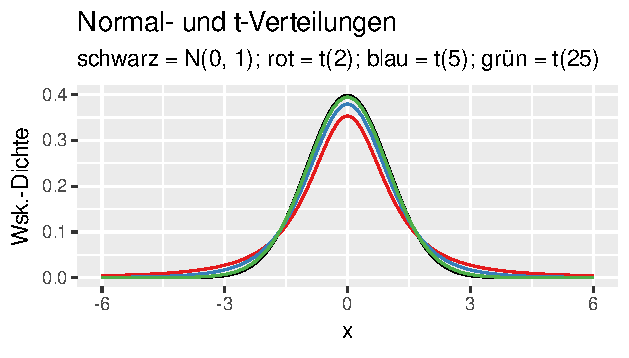
\includegraphics[width=.5\textwidth]{figs/unnamed-chunk-154-1} 

}

\caption{Eine Standardnormalverteilung und ein paar t-Verteilungen.\label{fig:tdistribution}}\label{fig:unnamed-chunk-154}
\end{figure}

\end{knitrout}

$t$-Verteilungen haben einen Parameter,
den man ihre Freiheitsgrade nennt.
Beim Schätzen eines Mittels ist die Anzahl Freiheitsgrade einfach
die Anzahl Beobachtungen minus 1: Gibt es 76 Beobachtungen,
gibt es 75 Freiheitsgrade. Abbildung \ref{fig:tdistribution} zeigt
$t$-Ver\-teil\-ung\-en mit 2, 5 und 25 Freiheitsgraden sowie
eine Standardnormalverteilung. Je mehr Freiheitsgrade,
desto ähnlicher ist die Verteilung einer Standardnormalverteilung.
Dies entspricht der Tatsache, dass grössere Stichproben $\sigma$
tendenziell weniger unterschätzen als kleinere Stichproben.

Um das 95\%-Konfidenzintervall um ein Stichprobenmittel mithilfe
der $t$-Verteilungen zu finden, sucht man zuerst das 2.5.\ und das
97.5.\ Perzentil der $t$-Verteilung mit $n-1$ Freiheitsgraden
(hier: $76-1=75$). Dann multipliziert man den geschätzten Standardfehler
mit diesen Perzentilen. Dies ist komplett analog zur Berechnung
auf der Basis des zentralen Grenzwertsatzes, nur wird mit einer
$t$- statt einer Normalverteilung gearbeitet.
\begin{knitrout}
\definecolor{shadecolor}{rgb}{0.969, 0.969, 0.969}\color{fgcolor}\begin{kframe}
\begin{alltt}
\hlstd{> }\hlkwd{qt}\hlstd{(}\hlnum{0.025}\hlstd{,} \hlkwc{df} \hlstd{=} \hlnum{75}\hlstd{)}
\end{alltt}
\begin{verbatim}
[1] -1.9921
\end{verbatim}
\begin{alltt}
\hlstd{> }\hlkwd{qt}\hlstd{(}\hlnum{0.975}\hlstd{,} \hlkwc{df} \hlstd{=} \hlnum{75}\hlstd{)}
\end{alltt}
\begin{verbatim}
[1] 1.9921
\end{verbatim}
\end{kframe}
\end{knitrout}

\begin{knitrout}
\definecolor{shadecolor}{rgb}{0.969, 0.969, 0.969}\color{fgcolor}\begin{kframe}
\begin{alltt}
\hlstd{> }\hlkwd{mean}\hlstd{(d}\hlopt{$}\hlstd{GJT)} \hlopt{+} \hlkwd{c}\hlstd{(}\hlopt{-}\hlnum{1.99}\hlstd{,} \hlnum{1.99}\hlstd{)} \hlopt{*} \hlkwd{sd}\hlstd{(d}\hlopt{$}\hlstd{GJT)} \hlopt{/} \hlkwd{sqrt}\hlstd{(}\hlnum{76}\hlstd{)}
\end{alltt}
\begin{verbatim}
[1] 144.54 157.01
\end{verbatim}
\end{kframe}
\end{knitrout}

In diesem Beispiel ergeben alle Berechungsmethoden
ein recht ähnliches Ergebnis. Insbesondere bei
kleinen Stichproben oder bei Stichproben, die den
Verdacht nahelegen, dass die Population sehr schräg
verteilt ist, ist dies aber nicht unbedingt der Fall.

Bemerken Sie, dass von den drei Methoden
die $t$-Methode die meisten Annahmen macht:
Sie geht nicht nur davon aus, dass man anhand
der Stichprobe sinnvolle Aussagen über die Unsicherheit machen kann
und dass die Population irgendwelche Verteilung hat,
für die den zentralen Grenzwertsatz bei dieser Stichprobengrösse greift,
sondern auch, dass die Population \emph{selber} normalverteilt ist.
Wenn all diese Annahmen aber stimmen, ist diese Methode auch
die genauste. Der Bootstrap dahingegen ist sozusagen
das Schweizer Sackmesser\footnote{Tatsächlich heisst der Vorläufer des Bootstraps das \textit{jackknife}.} unter den Schätzungsmethoden:
Er kann in vielen Situationen angewandt werden,
aber je nach Situation gibt es spezialisierte Methoden,
die schon besser funktionieren.

\section{Konfidenzintervalle}\label{sec:ci}
Im Laufe dieses Kapitels haben wir ein paar Konfidenzintervalle
konstruiert, sodass es nun die höchste Zeit ist, zu erklären,
was diese überhaupt sind. Eine leider schwierige Definition ist
die folgende:
\begin{quote}
Ein $\alpha$\%-Konfidenzintervall um ein
Stichprobenmittel besteht aus zwei Werten, die um dieses
Stichprobenmittel liegen und die nach einem bestimmten Verfahren
gewählt wurden, welches garantiert, dass
das Intervall das wahre Populationsmittel
($\mu$) in $\alpha$\% der Fälle enthält.
\end{quote}

Zum Beispiel werden 95\%-Konfidenzintervalle nach einem Verfahren
konstruiert, das garantieren soll, dass wenn man eine grosse
Anzahl Stichproben aus der Population zieht und für jede Stichprobe
das Intervall berechnet, 95\% dieser Intervalle $\mu$ enthalten.

Wie diese Definition zeigt, ist das Konzept schwieriger als was man auf den ersten Blick denken würde -- auch für erfahrene Forschende \citep{Hoekstra2014}. Oft interpretiert man ein 95\%-Konfidenzintervall als jene zwei Werte, zwischen denen der Populationsparameter (hier: $\mu$) mit 95\% Wahrscheinlichkeit liegt. Dies stimmt aber nicht \citep{Morey2016}.
Nichtsdestoweniger schreibt \citet{Ehrenberg1982} zur Interpretation
von Konfidenzintervallen Folgendes:
\begin{quote}
``[T]he rough-and-ready interpretation of confidence limits \dots will be close
to the truth. The choice is between making a statement which is true but so
complex that it is almost unactionable, and making one which is much simpler
but not quite correct. Fortunately, the effective content of the two kinds
of statement is generally similar.'' (S.\ 125)
\end{quote}

Statt Konfidenzintervallen empfehlen
\citet{Morey2016} den Gebrauch
von `Kredibilitätsintervallen'. Diese sind
in der bayesschen Statistik
angesiedelt und kommen momentan in
unserer Forschungsliteratur kaum vor,
weshalb ich sie hier nicht bespreche.
\citet{Albers2018} bemerken, dass Konfidenz- und
Kredibilitätsintervalle einander üblicherweise sehr ähnlich sind;
\citet{Nalborczyk2018} ziehen diese Schlussfolgerung aber in Frage.

Dieser Bemerkung zum Trotz sind meines Erachtens insbesondere die
folgenden Punkte wichtig:
\begin{itemize}
 \item Konfidenzintervalle heben hervor, dass Schätzungen inhärent unsicher sind.

 \item Bei grossen Stichproben oder bei Stichproben aus
 Populationen, in denen es wenig Variation gibt, sind Konfidenzintervalle
 tendenziell schmaler.

 \item Rein durch Zufall kann eine Stichprobe die Streuung
 in der Population unterschätzen und daher kann das Konfidenzintervall
 die Unsicherheit in der Schätzung ebenso unterschätzen.

 \item Genauere Unsicherheitseinschätzungen erhält man mit
 grösseren Stichproben oder indem man weitere nützliche Annahmen
 über die Daten macht (wie in der bayesschen Statistik).
\end{itemize}

Unter \url{https://rpsychologist.com/d3/CI/} finden Sie
eine lehrreiche App zu Konfidenzintervallen. Unter anderem
zeigt die App, dass Konfidenzintervalle manchmal schmal
sein können, aber die Schätzung trotzdem weit
vom Populationswert entfernt liegen kann.

\section{Aufgaben}
Es kommt eher selten vor, dass man das Mittel, den Median
oder die Standardabweichung (usw.) einer Population schätzen muss.
Stattdessen schätzt man in der Regel Unterschiede zwischen Gruppen
oder Zusammenhänge zwischen Variablen. Für solche Fälle werden
die gleichen Prinzipien wie jene in diesem Kapitel zutreffen,
aber es scheint mir Beschäftigungstherapie zu sein, weitere praktische
Aufgaben für dieses Kapitel zu erledigen. Stattdessen folgen
hier ein paar Denkaufgaben.

\begin{enumerate}
 \item Welche Faktoren bestimmen die tatsächliche Unsicherheit
 einer Parameterschätzung (z.B.\ eines Mittels)?

 \item Wie könnte man als ForscherIn die Unsicherheit bei der
 Schätzung verringern?

  \item Zwei Stichproben haben identische Stichprobenstandardabweichungen:
 $s_1 = s_2$. Stichprobe 1 bestehe aus 16 Datenpunkten; Stichprobe 2 aus nur vier.
 Aus welchen \emph{zwei} Gründen wird das 95\%-Konfidenzintervall
 bei Stichprobe 1 schmaler sein als bei Stichprobe 2, wenn Sie
 diese Intervalle mit $t$-Verteilungen konstruieren?

 \item Beim Arbeiten mit $t$-Verteilungen geht man davon aus,
 dass die Population, aus der die Stichprobe stammt, normalverteilt ist.
 Warum?

 \item Warum ist diese Normalitätsannahme weniger wichtig bei
 grösseren Stichproben?

 \item Auf Seite \pageref{par:trimmed} mussten Sie ein Konfidenzintervall um ein getrimmtes Mittel konstruieren.
 Dazu mussten Sie dazu Bootstrap-Stichproben mit je 76 Beobachtungen
 generieren und dann das 20\%-getrimmte Mittel dieser Stichproben berechnen.
 Wäre es stattdessen auch sinnvoll gewesen, zuerst die
 die 20\% niedrigsten und 20\% höchsten Werte aus der Stichprobe zu entfernen
 und anschliessend Bootstrap-Stichproben aus der restlichen Datenmenge von 46
 Beobachtungen zu generieren und bei diesen das normale Mittel zu berechnen?

\end{enumerate}


\chapter{Ein anderer Blick aufs Mittel}\label{ch:linmod}
In diesem und den folgenden Kapiteln behandeln wir das
sog.\ \textbf{allgemeine lineare Modell}
(\textit{general linear model}).\footnote{Nicht zu verwechseln
mit dem \textbf{verallgemeinerten linearen Modell}
(\textit{generalized linear model}).
Dieses ist eine Erweiterung des allgemeinen linearen Modells, 
mit der wir uns in diesem Kurs nur kurz befassen; siehe Kapitel \ref{ch:logistic}.}
Das allgemeine lineare Modell ist eine Methode,
um zu auszudrücken, wie ein oder mehrere \textbf{Prädiktoren}
mit dem \textbf{\textit{outcome}} zusammenhängen.
Oft redet man statt von Prädiktoren und outcome
von unabhängigen bzw.\ abhängigen Variablen,
aber ich finde die Begriffe Prädiktor und outcome
deutlicher.

In diesem Kapitel werden einige Schlüsselkonzepte des
allgemeinen linearen Modells erläutert, indem wir das
Mittel einer Population auf eine andere Art und Weise
schätzen als wir es bisher gemacht haben. 
In den darauf folgenden Kapiteln werden die
Modelle graduell komplexer, aber die Basisprinzipien
aus diesem Kapitel werden noch immer zutreffen.

\section{Ein Modell für die GJT-Daten}
Lasst uns kurz alles über Mittelwerte vergessen.
Wir erhalten Daten (hier: die GJT-Werte von \citet{DeKeyser2010},
siehe letztes Kapitel) und müssen
diese sinnvoll beschreiben. Sinnvoller als einfach
alle Datenpunkte aufzulisten, wäre, die Datenpunkte
in zwei Teile zu zerlegen: einen systematischen Teil, der die
Gemeinsamkeiten zwischen allen Werten ausdrückt,
und einen unsystematischen Teil, der die individuellen Unterschiede
zwischen diesen Gemeinsamkeiten und den Werten ausdrückt:
\[
\textrm{Wert einer Beobachtung} = \textrm{Gemeinsamkeit} + \textrm{Abweichung}.
\]
Um die Notation übersichtlich zu halten, wird diese Gleichung
meistens so geschrieben:
\begin{equation}\label{eq:beta0}
 y_i = \beta_0 + \varepsilon_i.
\end{equation}
Hier ist $y_i$ die i.\ Beobachtung im Datensatz,
$\beta_0$ stellt die Gemeinsamkeit zwischen allen
Werten in der Population dar
und $\varepsilon_i$ drückt aus, wie stark
die i.\ Beobachtung von diesem Populationswert abweicht.
$\varepsilon_i$ nennt man auch die \textbf{Residuen}
oder den \textbf{Restfehler}.
Wir schreiben $\beta_0$ statt einfach $\beta$,
weil wir nachher die Gemeinsamkeit
zwischen den $y$-Werten mithilfe mehrerer
$\beta$s ausdrücken werden.

In der Regel interessieren wir uns mehr für die $\beta$s
als für die $\varepsilon$s.
Da uns aber nicht die ganze Population
zur Verfügung steht, müssen wir uns mit einer Schätzung
von $\beta_0$ begnügen.
In Gleichung \ref{eq:beta0} ist $\beta_0$ ein Parameter
mit einem bestimmten, aber in der Regel unbekannten Wert;
für Schätzungen dieses Parameters wird die Notation
$\widehat{\beta_0}$ verwendet.
Da $\widehat{\beta_0}$ bloss eine Schätzung ist,
wird der Restfehler ebenfalls bloss geschätzt:
\[
y_i = \widehat{\beta_0} + \widehat{\varepsilon_i}.
\]

Wie können wir nun $\widehat{\beta_0}$ berechnen
(bzw.\ $\beta_0$ schätzen)?
Im Prinzip geht die Gleichung für jeden $\beta_0$-Wert
auf, denn wir können uns die $\widehat{\varepsilon}$-Werte
eben so aussuchen, wie es uns passt.
Die ersten beiden GJT-Werte im Datensatz sind
151 und 182. Wenn wir nun beispielsweise für $\beta_0$ einen beliebligen
Wert, z.B.\ 1823, wählen,
wählen wir $\widehat{\varepsilon_1} = -1672$ und $\widehat{\varepsilon_2} = -1641$ und die Gleichung geht auf:
\[
y_1 = 151 = 1823 - 1672,
\]
\[
y_2 = 182 = 1823 - 1641.
\]
Wenn wir nun für $\beta_0$ den
Wert 14 wählen, wählen wir $\widehat{\varepsilon_1} = 137$ und $\widehat{\varepsilon_2} = 168$
und die Gleichung geht wiederum auf:
\[
y_1 = 151 = 14 + 137,
\]
\[
y_2 = 182 = 14 + 168.
\]
Wir brauchen also eine prinzipielle Methode, um
$\beta_0$ zu schätzen.

\section{Die Methode der kleinsten Quadrate}
Die Frage stellt sich, was die optimale Art und Weise
ist, um $\widehat{\beta_0}$ zu bestimmen.
Die wenig überraschende Antwort lautet: Es hängt davon
ab, was man unter `optimal' versteht.
Eine sinnvolle Definition von `optimal' ist,
dass $\beta_0$ so geschätzt werden soll, dass
die Summe der absoluten Restfehler
($\sum_{i = 1}^{n} |\widehat{\varepsilon_i}|$) möglichst klein ist.
Wenn wir für $\widehat{\beta_0}$ den Wert 135 wählen,
beträgt die Summe der absoluten Restfehler 1993.
Hier gehen wir davon aus, dass der Datensatz 
\texttt{dekeyser2010.csv} als den Objektnamen \texttt{d} hat.

\begin{knitrout}
\definecolor{shadecolor}{rgb}{0.969, 0.969, 0.969}\color{fgcolor}\begin{kframe}
\begin{alltt}
\hlstd{> }\hlkwd{sum}\hlstd{(}\hlkwd{abs}\hlstd{(d}\hlopt{$}\hlstd{GJT} \hlopt{-} \hlnum{135}\hlstd{))}
\end{alltt}
\begin{verbatim}
[1] 1993
\end{verbatim}
\end{kframe}
\end{knitrout}
(Bemerken Sie, dass $y_i = \widehat{\beta_0} + \widehat{\varepsilon_i}$, also $\widehat{\varepsilon_i} = y_i - \widehat{\beta_0}$.)

Wenn wir stattdessen den Wert 148 wählen, beträgt die Summe der absoluten Restfehler 1799.
\begin{knitrout}
\definecolor{shadecolor}{rgb}{0.969, 0.969, 0.969}\color{fgcolor}\begin{kframe}
\begin{alltt}
\hlstd{> }\hlkwd{sum}\hlstd{(}\hlkwd{abs}\hlstd{(d}\hlopt{$}\hlstd{GJT} \hlopt{-} \hlnum{148}\hlstd{))}
\end{alltt}
\begin{verbatim}
[1] 1799
\end{verbatim}
\end{kframe}
\end{knitrout}

Wenn wir `optimal' so definieren, ist 148 also die bessere
Schätzung von $\beta_0$. Diese Übung können wir für jede Menge
Kandidatwerte durchprobieren und dann den optimalen Wert wählen.
Dies ist die \textbf{Methode der kleinsten absoluten Abweichungen}.
Wie Abbildung \ref{fig:optimisation} (links)
zeigt, sind $\beta_0$-Schätzungen
zwischen 150 und 151 in diesem Sinne optimal.
Der Median der GJT-Werte ist nicht zufällig 150.5: Wenn man $\beta_0$
mit der Methode der kleinsten absoluten Abweichungen schätzt, ist
das Ergebnis der Median der Stichprobe.
Dass wir es hier mit einer Schätzung zu tun haben,
wird klar, wenn man sich überlegt, dass diese Methode
ein anderes Ergebnis liefern könnte, wenn man eine neue
Stichprobe aus der gleichen Population zieht.

\begin{knitrout}
\definecolor{shadecolor}{rgb}{0.969, 0.969, 0.969}\color{fgcolor}\begin{figure}[tp]

{\centering 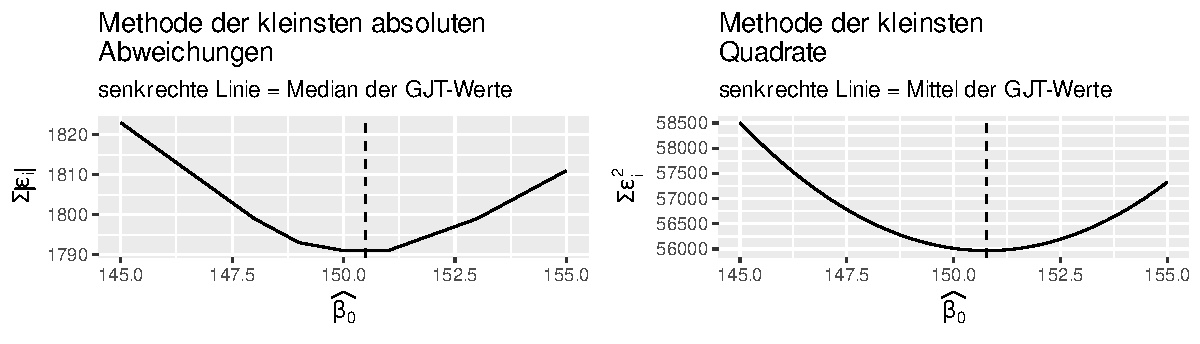
\includegraphics[width=.9\textwidth]{figs/unnamed-chunk-159-1} 

}

\caption{Links: Wenn der Parameter mit der Methode der kleinsten absoluten Abweichungen geschätzt wird, ist die Lösung gleich dem Median der Stichprobe. Rechts: Wenn der Parameter mit der Methode der kleinsten Quadrate geschätzt wird, ist die Lösung gleich dem Mittel der Stichprobe. \label{fig:optimisation}}\label{fig:unnamed-chunk-159}
\end{figure}

\end{knitrout}

Eine andere sinnvolle Definition von `optimal' ist,
dass $\beta_0$ so geschätzt werden soll, dass
die Summe der quadrierten Restfehler
($\sum_{i = 1}^{n} \widehat{\varepsilon_i}^2$) möglichst klein ist.
Dies ist die \textbf{Methode der kleinsten Quadrate}.
Verglichen mit der Methode der kleinsten absoluten Abweichungen
fallen grosse Residuen noch mehr ins Gewicht.
Anders gesagt: Grosse Abweichungen (darunter auch Ausreisser) üben
einen stärkeren Einfluss auf das Ergebnis aus.
Wie Abbildung \ref{fig:optimisation} (rechts) zeigt,
ist die optimal $\beta_0$-Schätzung laut der Methode
der kleinsten Quadrate 150.78---nicht zufällig das Mittel
der Stichprobe!

Während wir in Kapitel 3 die Summe der Quadrate als eine
Funktion des Mittels betrachtet haben, kann man die Rollen
auch umkehren: Das Mittel ist jener Wert, der die Summe
der Quadrate minimiert. Ebenso ist der Median jener Wert,
der die Summe der absoluten Abweichungen minimiert.
Der Modus ist übrigens der Wert, der die Summe der binären 
Abweichungen minimiert. 
Sind $y_i$ und $\widehat{\beta_0}$ einander gleich, beträgt 
die binäre Abweichung 0, sonst 1.

Rechnerisch ist die Methode der kleinsten Quadrate am einfachsten,
und die Parameter in allgemeinen linearen Modellen werden daher
meistens mit dieser Methode geschätzt
(\textit{ordinary least squares}, OLS).
Aber dies ist keine Notwendigkeit.
In bestimmten Bereichen trifft man ab und zu andere Optimierungskriterien an;
in den Sprachwissenschaften ist dies aber selten der Fall.
Im Prinzip kann man sogar selber Optimierungskriterien
definieren, aber dies kommt noch weniger vor.

\section{Lineare Modelle in R}
Mit der \texttt{lm()}-Funktion können lineare Modelle aufgebaut werden.
Ihre Parameter werden anhand der Methode der kleinsten Quadrate geschätzt.
Innerhalb der Funktion braucht es eine Formel mit dem outcome
vor und den Prädiktoren nach der Tilde. In diesem Fall gibt es keinen
Prädiktor, stattdessen wird \texttt{1} verwendet.




\begin{knitrout}
\definecolor{shadecolor}{rgb}{0.969, 0.969, 0.969}\color{fgcolor}\begin{kframe}
\begin{alltt}
\hlstd{> }\hlstd{mod.lm} \hlkwb{<-} \hlkwd{lm}\hlstd{(GJT} \hlopt{~} \hlnum{1}\hlstd{,} \hlkwc{data} \hlstd{= d)}
\end{alltt}
\end{kframe}
\end{knitrout}

Die geschätzten $\beta$s kann man abrufen, indem
man den Namen des Modells (hier: \texttt{mod.lm})
eintippt.

\begin{knitrout}
\definecolor{shadecolor}{rgb}{0.969, 0.969, 0.969}\color{fgcolor}\begin{kframe}
\begin{alltt}
\hlstd{> }\hlstd{mod.lm}
\end{alltt}
\begin{verbatim}

Call:
lm(formula = GJT ~ 1, data = d)

Coefficients:
(Intercept)  
      150.8  
\end{verbatim}
\end{kframe}
\end{knitrout}

Auch mit \texttt{coef()} erhält man die $\beta$-Schätzungen (hier nur $\beta_0$).

\begin{knitrout}
\definecolor{shadecolor}{rgb}{0.969, 0.969, 0.969}\color{fgcolor}\begin{kframe}
\begin{alltt}
\hlstd{> }\hlkwd{coef}\hlstd{(mod.lm)}
\end{alltt}
\begin{verbatim}
(Intercept) 
   150.7763 
\end{verbatim}
\end{kframe}
\end{knitrout}

Dass mal 150.8 und mal 150.7763 angezeigt wird, liegt lediglich daran, dass das der Output
der letzten zwei Befehle strenger bzw.\ lockerer gerundet wird.

Mit \texttt{predict()} erhält man einen Vektor mit $n$ Werten (hier: $n = 76$),
der die `vorhergesagten' $y$-Werte enthält.
(Ich mag den Begriff `vorhergesagt' hier nicht.)
Es handelt sich um die $y$-Werte abzüglich der $\hat{\varepsilon}$-Werte: $\widehat{y_i} = y_i - \widehat{\varepsilon_i}$.
In unserem Fall sind dies lediglich 76 Wiederholungen von $\widehat{\beta_0}$.\footnote{$y_i = \widehat{\beta_0} + \widehat{\varepsilon_i}$. Also $\widehat{\varepsilon_i} = y_i - \widehat{\beta_0}$, also $\widehat{y_i} = y_i - \widehat{\varepsilon_i} = y_i - (y_i - \widehat{\beta_0}) =  \widehat{\beta_0}$.}

\begin{knitrout}
\definecolor{shadecolor}{rgb}{0.969, 0.969, 0.969}\color{fgcolor}\begin{kframe}
\begin{alltt}
\hlstd{> }\hlkwd{predict}\hlstd{(mod.lm)}
\end{alltt}
\begin{verbatim}
       1        2        3        4        5        6 
150.7763 150.7763 150.7763 150.7763 150.7763 150.7763 
       7        8        9       10       11       12 
150.7763 150.7763 150.7763 150.7763 150.7763 150.7763 
      13       14       15       16       17       18 
150.7763 150.7763 150.7763 150.7763 150.7763 150.7763 
      19       20       21       22       23       24 
150.7763 150.7763 150.7763 150.7763 150.7763 150.7763 
      25       26       27       28       29       30 
150.7763 150.7763 150.7763 150.7763 150.7763 150.7763 
      31       32       33       34       35       36 
150.7763 150.7763 150.7763 150.7763 150.7763 150.7763 
      37       38       39       40       41       42 
150.7763 150.7763 150.7763 150.7763 150.7763 150.7763 
      43       44       45       46       47       48 
150.7763 150.7763 150.7763 150.7763 150.7763 150.7763 
      49       50       51       52       53       54 
150.7763 150.7763 150.7763 150.7763 150.7763 150.7763 
      55       56       57       58       59       60 
150.7763 150.7763 150.7763 150.7763 150.7763 150.7763 
      61       62       63       64       65       66 
150.7763 150.7763 150.7763 150.7763 150.7763 150.7763 
      67       68       69       70       71       72 
150.7763 150.7763 150.7763 150.7763 150.7763 150.7763 
      73       74       75       76 
150.7763 150.7763 150.7763 150.7763 
\end{verbatim}
\end{kframe}
\end{knitrout}

Die Residuen kann man mit der \texttt{resid()}-Funktion abfragen.

\begin{knitrout}
\definecolor{shadecolor}{rgb}{0.969, 0.969, 0.969}\color{fgcolor}\begin{kframe}
\begin{alltt}
\hlstd{> }\hlcom{# Output hier nicht gezeigt}
\hlstd{> }\hlkwd{resid}\hlstd{(mod.lm)}
\end{alltt}
\end{kframe}
\end{knitrout}

\section{Unsicherheit in einem allgemeinen linearen Modell quantifizieren}

\subsection{Der Bootstrap}
Genauso wie im letzten Kapitel können wir den Bootstrap
verwenden, um die Unsicherheit in der Schätzung von $\beta_0$
zu quantifizieren. Da in diesem Fall $\widehat{\beta_0} = \bar{x}$,
ergibt dies natürlich die gleiche Lösung wie vorher. Aber es gibt
mir die Gelegenheit, zu zeigen, wie man auch für komplexere
lineare Modelle den Bootstrap verwenden kann.

Die Logik ist wiederum, dass wir die Stichprobe stellvertretend
für die Population einsetzen. Aber anstatt Bootstrap-Stichproben
aus der Stichprobe zu ziehen, ziehen wir diesmal Bootstrap-Stichproben
aus den Residuen ($\varepsilon$). Diese kombinieren wir dann
mit $\widehat{\beta_0}$, um die Bootstrap-Stichproben zu generieren.
Wenn wir uns nur fürs Mittel interessieren, hat diese Methode
überhaupt keinen Mehrwert, denn sie ist mathematisch der zuerst
besprochenen Bootstrap-Methode gleich. Aber sie ist pädagogisch wertvoller
(und manchmal auch statistisch besser),
wenn wir später mehrere $\beta$s haben werden.
Konkret:
\begin{enumerate}\label{bootstrapoverview}
 \item Man berechnet $\widehat{\beta_0}$ und erhält dazu auch noch
 einen Vektor $\hat{\varepsilon}$, der die Werte
 $\widehat{\varepsilon_1}$ bis $\widehat{\varepsilon_n}$ enthält.
 \item Man zieht eine Bootstrap-Stichprobe aus $\hat{\varepsilon}$ (\textit{sampling with replacement}).
 Diese kann man als $\hat{\varepsilon}^{*}$ bezeichnen.
 Dieser Vektor enthält ebenso $n$ Werte,
 wobei bestimmte $\widehat{\varepsilon_i}$ eventuell 
 nicht vorkommen, andere dafür mehrmals.
 \item Man kombiniert $\widehat{\beta_0}$ und $\hat{\varepsilon}^{*}$. Dies ergibt
 eine neue Reihe von $y$-Werten: $y_i^{*} = \widehat{\beta_0} + \widehat{\varepsilon_i}^{*}$.
 \item Man schätzt nun auf der Basis von $y^{*}$ erneut den Parameter von Interesse ($\widehat{\beta_0}^{*}$).
 \item Man führt Schritte 2--4 ein paar tausend Mal aus und erhält so die Verteilung
 der gebootstrappten $\beta_0$-Schätzungen.
\end{enumerate}

Der unten stehende R-Code implementiert diese Schritte.
\begin{knitrout}
\definecolor{shadecolor}{rgb}{0.969, 0.969, 0.969}\color{fgcolor}\begin{kframe}
\begin{alltt}
\hlstd{> }\hlstd{n_bootstrap} \hlkwb{<-} \hlnum{20000}
\hlstd{> }\hlstd{bs_b0} \hlkwb{<-} \hlkwd{vector}\hlstd{(}\hlkwc{length} \hlstd{= n_bootstrap)}
\hlstd{> }
\hlstd{> }\hlkwa{for} \hlstd{(i} \hlkwa{in} \hlnum{1}\hlopt{:}\hlstd{n_bootstrap) \{}
\hlstd{+ }  \hlcom{# Residuen bootstrappen}
\hlstd{+ }  \hlstd{bs_residual} \hlkwb{<-} \hlkwd{sample}\hlstd{(}\hlkwd{resid}\hlstd{(mod.lm),} \hlkwc{replace} \hlstd{=} \hlnum{TRUE}\hlstd{)}

\hlstd{+ }  \hlcom{# neuen Outcome kreieren}
\hlstd{+ }  \hlstd{bs_outcome} \hlkwb{<-} \hlkwd{predict}\hlstd{(mod.lm)} \hlopt{+} \hlstd{bs_residual}

\hlstd{+ }  \hlcom{# Modell neu berechnen mit diesem Outcome}
\hlstd{+ }  \hlstd{bs_mod} \hlkwb{<-} \hlkwd{lm}\hlstd{(bs_outcome} \hlopt{~} \hlnum{1}\hlstd{)}

\hlstd{+ }  \hlcom{# Schätzung speichern}
\hlstd{+ }  \hlstd{bs_b0[[i]]} \hlkwb{<-} \hlkwd{coef}\hlstd{(bs_mod)[[}\hlnum{1}\hlstd{]]}
\hlstd{+ }\hlstd{\}}
\end{alltt}
\end{kframe}
\end{knitrout}

Wir können jetzt wieder die Verteilung der
gebootstrappten Parameterschätzungen visualisieren,
und ihre Standardabweichung und 2.5.\ und 97.5.\ Perzentile
berechnen. Die Ergebnisse sind natürlich identisch
mit jenen aus Kapitel \ref{ch:uncertainty}.

\begin{knitrout}
\definecolor{shadecolor}{rgb}{0.969, 0.969, 0.969}\color{fgcolor}\begin{kframe}
\begin{alltt}
\hlstd{> }\hlcom{# Das Histogramm wird hier nicht gezeigt.}
\hlstd{> }\hlkwd{hist}\hlstd{(bs_b0)}
\end{alltt}
\end{kframe}
\end{knitrout}

\begin{knitrout}
\definecolor{shadecolor}{rgb}{0.969, 0.969, 0.969}\color{fgcolor}\begin{kframe}
\begin{alltt}
\hlstd{> }\hlkwd{sd}\hlstd{(bs_b0)}
\end{alltt}
\begin{verbatim}
[1] 3.103987
\end{verbatim}
\begin{alltt}
\hlstd{> }\hlkwd{quantile}\hlstd{(bs_b0,} \hlkwc{probs} \hlstd{=} \hlkwd{c}\hlstd{(}\hlnum{0.025}\hlstd{,} \hlnum{0.975}\hlstd{))}
\end{alltt}
\begin{verbatim}
    2.5%    97.5% 
144.7105 156.8687 
\end{verbatim}
\end{kframe}
\end{knitrout}
 
\subsection{Ein anderer Bootstrap}\label{semiparametricbootstrap}
Beim Bootstrap, den wir soeben besprochen haben,
sind wir davon ausgegangen, dass die Residuen
in der Stichprobe genau so verteilt sind wie die
Residuen in der Population. Ein Nachteil dieser
Annahme ist, dass wir dadurch die Feinkörnigkeit
der Residuen in der Population wohl unterschätzen.
Beispielsweise gibt es für das \texttt{mod.lm}-Modell
ein Residuum von $-14.78$ und ein Residuum von
$-12.78$, aber keines von $-13.78$.
Ein Residuum von $-14.78$ entspricht einer Beobachtung
von $150.78 - 14.78 = 136$; ein Residuum von $-13.78$
entspräche einer Beobachtung von $150.78 - 13.78 = 137$.
Nach unserer Annahme gäbe es in der Population also
keine Versuchspersonen mit einem GJT-Ergebnis von 137.

Dies ist natürlich eine etwas komische Annahme;
in der Regel hat sie aber kaum einen Einfluss auf die
Inferenzen. Aber eine Alternative wäre,
dass wir davon ausgingen, dass die Residuen in
der Population normalverteilt sind. Normalverteilungen
sind unendlich feinkörnig, sodass diese Annahme sozusagen
den Gegenpol der ersten Annahme darstellt.
Das Mittel der Residuen beträgt 0, sodass
wir nur die Standardabweichung der normalverteilten Restfehler
in der Population
finden müssen. Diese wird durch die Standardabweichung
der Restfehler in der Stichprobe geschätzt.
Dafür können wir hier zwei Funktionen verwenden:

\begin{knitrout}
\definecolor{shadecolor}{rgb}{0.969, 0.969, 0.969}\color{fgcolor}\begin{kframe}
\begin{alltt}
\hlstd{> }\hlkwd{sd}\hlstd{(}\hlkwd{resid}\hlstd{(mod.lm))}
\end{alltt}
\begin{verbatim}
[1] 27.31769
\end{verbatim}
\begin{alltt}
\hlstd{> }\hlkwd{sigma}\hlstd{(mod.lm)}
\end{alltt}
\begin{verbatim}
[1] 27.31769
\end{verbatim}
\end{kframe}
\end{knitrout}

In diesem Beispiel (lineares Modell ohne Prädiktoren)
sind diese Werte identisch, aber sobald Prädiktoren
im Spiel sind, liefert \texttt{sigma()} die bessere Schätzung
der Standardabweichung der Residuen. Sie wird so berechnet:
\begin{equation}\label{eq:sigmap}
\widehat{\sigma_{\varepsilon}} = \sqrt{\frac{1}{n - p} \sum_{i = 1}^{n} \widehat{\varepsilon_i^2}},
\end{equation}
wo $p$ die
Anzahl geschätzten $\beta$s ist.
In diesem Fall ist $p = 1$, sodass die Gleichung die
Stich\-proben\-standard\-ab\-weichung der Residuen ergibt:
\begin{knitrout}
\definecolor{shadecolor}{rgb}{0.969, 0.969, 0.969}\color{fgcolor}\begin{kframe}
\begin{alltt}
\hlstd{> }\hlkwd{sqrt}\hlstd{(}\hlkwd{sum}\hlstd{(}\hlkwd{resid}\hlstd{(mod.lm)}\hlopt{^}\hlnum{2}\hlstd{)}\hlopt{/}\hlstd{(}\hlkwd{length}\hlstd{(}\hlkwd{resid}\hlstd{(mod.lm))} \hlopt{-} \hlkwd{length}\hlstd{(}\hlkwd{coef}\hlstd{(mod.lm))))}
\end{alltt}
\begin{verbatim}
[1] 27.31769
\end{verbatim}
\end{kframe}
\end{knitrout}
Hier teilt man durch $n-p$ aus dem gleichen Grund,
weshalb man bei der Standardabweichung der Beobachtungen
in der einer Stichprobe durch $n-1$ teilt: um eine systematische
Unterschätzung zum grössten Teil entgegenzuwirken.

Anstatt für jede Bootstrapstichprobe die Residuen
durch \textit{sampling with replacement} zu generieren,
werden sie hier zufällig aus einer Normalverteilung
mit $\mu = 0$ und $\sigma = \widehat{\sigma_{\varepsilon}}$ generiert:

\begin{knitrout}
\definecolor{shadecolor}{rgb}{0.969, 0.969, 0.969}\color{fgcolor}\begin{kframe}
\begin{alltt}
\hlstd{> }\hlstd{n_bootstrap} \hlkwb{<-} \hlnum{20000}
\hlstd{> }\hlstd{bs_b0} \hlkwb{<-} \hlkwd{vector}\hlstd{(}\hlkwc{length} \hlstd{= n_bootstrap)}
\hlstd{> }
\hlstd{> }\hlkwa{for} \hlstd{(i} \hlkwa{in} \hlnum{1}\hlopt{:}\hlstd{n_bootstrap) \{}
\hlstd{+ }  \hlcom{# Neue Residuen aus Normalverteilung generieren}
\hlstd{+ }  \hlstd{bs_residual} \hlkwb{<-} \hlkwd{rnorm}\hlstd{(}\hlkwc{n} \hlstd{=} \hlnum{76}\hlstd{,} \hlkwc{sd} \hlstd{=} \hlkwd{sigma}\hlstd{(mod.lm))}

\hlstd{+ }  \hlcom{# neuen Outcome kreieren}
\hlstd{+ }  \hlstd{bs_outcome} \hlkwb{<-} \hlkwd{predict}\hlstd{(mod.lm)} \hlopt{+} \hlstd{bs_residual}

\hlstd{+ }  \hlcom{# Modell neu berechnen mit diesem Outcome}
\hlstd{+ }  \hlstd{bs_mod} \hlkwb{<-} \hlkwd{lm}\hlstd{(bs_outcome} \hlopt{~} \hlnum{1}\hlstd{)}

\hlstd{+ }  \hlcom{# Schätzung speichern}
\hlstd{+ }  \hlstd{bs_b0[[i]]} \hlkwb{<-} \hlkwd{coef}\hlstd{(bs_mod)[}\hlnum{1}\hlstd{]}
\hlstd{+ }\hlstd{\}}
\end{alltt}
\end{kframe}
\end{knitrout}

\begin{knitrout}
\definecolor{shadecolor}{rgb}{0.969, 0.969, 0.969}\color{fgcolor}\begin{kframe}
\begin{alltt}
\hlstd{> }\hlcom{# Histogramm (nicht gezeigt)}
\hlstd{> }\hlkwd{hist}\hlstd{(bs_b0)}
\end{alltt}
\end{kframe}
\end{knitrout}


\begin{knitrout}
\definecolor{shadecolor}{rgb}{0.969, 0.969, 0.969}\color{fgcolor}\begin{kframe}
\begin{alltt}
\hlstd{> }\hlcom{# Geschätzter Standardfehler}
\hlstd{> }\hlkwd{sd}\hlstd{(bs_b0)}
\end{alltt}
\begin{verbatim}
[1] 3.129119
\end{verbatim}
\begin{alltt}
\hlstd{> }\hlcom{# 95% Konfidenzintervall}
\hlstd{> }\hlkwd{quantile}\hlstd{(bs_b0,} \hlkwc{probs} \hlstd{=} \hlkwd{c}\hlstd{(}\hlnum{0.025}\hlstd{,} \hlnum{0.975}\hlstd{))}
\end{alltt}
\begin{verbatim}
    2.5%    97.5% 
144.5470 156.9135 
\end{verbatim}
\end{kframe}
\end{knitrout}

Diese Art von Bootstrap---bei der wir davon ausgehen,
dass die Residuen eine bestimmte Verteilung haben,
und wir die relevanten Parameter dieser Verteilung
anhand der Stichprobe schätzen---nennt man
einen \textbf{parametrischen Bootstrap}.
Den Bootstrap aus dem letzten Abschnitt---bei der man
Bootstrapstichproben der Modellresiduen
mit den Modellvorhersagen kombiniert und die relevanten
Parameter anhand dieser neuen Werte schätzt---nennt
man einen \textbf{semiparametrischen Bootstrap}.
Den Bootstrap aus dem letzten Kapitel---bei der man
Bootstrapstichproben aus dem ursprünglichen Datensatz
generiert---nennt man einen \textbf{nichtparametrischen Bootstrap}.
% Siehe auch \href{https://janhove.github.io/teaching/2016/12/20/bootstrapping}{\textit{Some illustrations of bootstrapping}} (20.12.2016).

Man bemerke hier übrigens, dass sowohl die Annahme,
dass die Residuen in der Population genau so wie in der Stichprobe
verteilt sind, als auch die Annahme, dass sie normalverteilt und
unendlich feinkörnig sind, hier gar nicht stimmen können,
da bei dieser Studie nur Ganzzahlen zwischen 0 und 204 hätten
vorkommen können. Die Tatsache, dass wir unter unterschiedlichen
Annahmen zum gleichen Ergebnis kommen, deutet bereits darauf hin, 
dass bei dieser Stichprobengrosse die Schätzung der Unsicherheit eines
Mittels
nicht massgeblich von Annahmen über die genaue Verteilung der
Residuen in der Population abhängt.

\subsection{Mit $t$-Verteilungen}
Wenn man ohnehin davon ausgehen will, dass die Residuen
normalverteilt sind, kann man den geschätzten
Standardfehler und das Konfidenzintervall
auch analytisch herleiten.
Die Formeln, die man dazu braucht, werden hier
nicht gezeigt, denn sie haben kaum einen didaktischen
Mehrwert.
In R kann man die \texttt{summary()}-Funktion
verwenden, um den geschätzten Standardfehler zu berechnen
(\texttt{Std. Error}):
\begin{knitrout}
\definecolor{shadecolor}{rgb}{0.969, 0.969, 0.969}\color{fgcolor}\begin{kframe}
\begin{alltt}
\hlstd{> }\hlkwd{summary}\hlstd{(mod.lm)}
\end{alltt}
\begin{verbatim}

Call:
lm(formula = GJT ~ 1, data = d)

Residuals:
    Min      1Q  Median      3Q     Max 
-46.776 -23.026  -0.276  23.224  47.224 

Coefficients:
            Estimate Std. Error t value Pr(>|t|)
(Intercept)  150.776      3.134   48.12   <2e-16

Residual standard error: 27.32 on 75 degrees of freedom
\end{verbatim}
\end{kframe}
\end{knitrout}
$\beta_0$ heisst hier \texttt{(Intercept)}.
Was \texttt{t value} und \texttt{Pr(>|t|)} bedeuten,
werden wir erst in einem späteren Kapitel besprechen.

Das 95\%-Konfidenzintervall kann mit \texttt{confint()}
berechnet werden.
\begin{knitrout}
\definecolor{shadecolor}{rgb}{0.969, 0.969, 0.969}\color{fgcolor}\begin{kframe}
\begin{alltt}
\hlstd{> }\hlkwd{confint}\hlstd{(mod.lm)}
\end{alltt}
\begin{verbatim}
              2.5 %   97.5 %
(Intercept) 144.534 157.0187
\end{verbatim}
\end{kframe}
\end{knitrout}

Natürlich kann man auch gerne andere Intervalle berechnen,
z.B.\ 80\%-Konfidenzintervalle:
\begin{knitrout}
\definecolor{shadecolor}{rgb}{0.969, 0.969, 0.969}\color{fgcolor}\begin{kframe}
\begin{alltt}
\hlstd{> }\hlkwd{confint}\hlstd{(mod.lm,} \hlkwc{level} \hlstd{=} \hlnum{0.80}\hlstd{)}
\end{alltt}
\begin{verbatim}
                10 %     90 %
(Intercept) 146.7248 154.8278
\end{verbatim}
\end{kframe}
\end{knitrout}


\paragraph{Denkaufgabe.}
Warum wird bei der \texttt{summary()}-Funktion
schon der Median aber nicht das Mittel der Residuen gezeigt?


\section{Fazit}

\begin{itemize}
\item Datenpunkte kann man als eine Kombination einer
Gemeinsamkeit aller Datenpunkte in der Population und einer
spezifischen Abweichung verstehen.
\item In der Regel ist die Gemeinsamkeit von Interesse;
diese wird aber anhand der Abweichungen und eines
Optimierungskriteriums geschätzt.
\item Das am meisten verwendetete Optimierungskriterium
ist die Methode der kleinsten Quadrate, die im `univariaten' Fall
(= wenn man nur mit einer Variablen arbeitet) das Mittel ergibt,
aber es existieren auch andere Methoden.
\item Die Unsicherheit in der Parameterschätzung kann
mithilfe des Bootstraps oder anhand weiterer Annahmen geschätzt werden.
\end{itemize}

\bigskip

Es gibt keine weiteren Aufgaben zu diesem Kapitel.

% \section{Aufgaben}
% Diese Aufgaben haben zum Ziel 
% \begin{enumerate}
%     \item Wie würden Sie den parametrischen Bootstrap fürs \texttt{mod.lm}-Modell
%   anpassen, wenn Sie davon ausgehen würden, dass die Residuen in der Population
%   aus einer kontinuierlichen Gleichverteilung statt aus einer Normalverteilung stammten? 
%   
%   \item Wie würden Sie die \texttt{min}- und \texttt{max}-Parameter der 
%   \texttt{runif()}-Funktion bestimmen? Sehen Sie dabei Probleme?
%   
%   \item Führen Sie das Bootstrapping unter dieser Annahme aus. Welche Schätzung erhalten
%   Sie für $\widehat{\sigma}_{\bar{x}}$?
%   
%   \item Wäre eine diskrete Gleichverteilung hier sinnvoller als eine kontinuierliche
%   Gleichverteilung? Welche Werte würden in dieser diskreten Gleichverteilung vorkommen?
% \end{enumerate}


\chapter{Einen Prädiktor hinzufügen}\label{ch:simpleregression}
In diesem Kapitel beschäftigen wir uns mit der Frage,
wie der Zusammenhang zwischen einem einzigen kontinuierlichen
Prädiktor und einem einzigen kontinuierlichen Outcome erfasst
werden kann. Eine \textbf{kontinuierliche} Variable ist eine
eher feinkörnige Variable, deren Werte geordnet werden können
(z.B.\ von klein nach gross oder von schlecht nach gut). Ausserdem
können Unterschiede auf der Skala sinnvoll miteinander verglichen
werden: Der Unterschied zwischen 15 und 20 °C ist gleich dem
Unterschied zwischen $-10$ und $-5$ °C,
und beide Unterschiede sind halb so gross wie jener
zwischen 50 und 60 °C. Diese Eigenschaften haben sowohl die
GJT- als auch die AOA-Variable im Datensatz von \citet{DeKeyser2010}.

In den letzten zwei Kapiteln haben wir uns mit der zentralen Tendenz
der GJT-Daten beschäftigt. Eigentlich interessierten sich \citet{DeKeyser2010}
aber nicht sosehr für diese, sondern für den Zusammenhang zwischen GJT und AOA.
Diesen Zusammenhang schauen wir uns hier an. Wie immer ist es eine gute
Idee, die Daten zunächst grafisch darzustellen.
Wenn man sich für den
Zusammenhang zwischen zwei kontinuierlichen Variablen interessiert,
bietet sich das \textbf{Streudiagramm} (\textit{scatterplot}) an;
siehe Abbildung \ref{fig:dekeyser}. Beim Zeichnen eines
Streudiagramms muss man spezifizieren, welche Variable entlang
der $x$-Achse und welche entlang der $y$-Achse dargestellt wird.
Wenn es naheliegender ist, dass Variable $A$ Variable $B$ beeinflusst
als umgekehrt, empfiehlt es sich, Variable $A$ entlang der $x$-Achse
darzustellen und Variable $B$ entlang der $y$-Achse. Hier ist es
unmöglich, dass die Grammatikalitätsurteile das Erwerbsalter
beeinflussen, aber sehr wohl, dass das Erwerbsalter die Grammatikalitätsurteile beeinflussen.

\begin{knitrout}
\definecolor{shadecolor}{rgb}{0.969, 0.969, 0.969}\color{fgcolor}\begin{kframe}
\begin{alltt}
\hlstd{> }\hlkwd{ggplot}\hlstd{(}\hlkwc{data} \hlstd{= d,}
\hlstd{+ }       \hlkwd{aes}\hlstd{(}\hlkwc{x} \hlstd{= AOA,}
\hlstd{+ }           \hlkwc{y} \hlstd{= GJT))} \hlopt{+}
\hlstd{+ }  \hlcom{# 'shape = 1' zeichnet leere Kreischen}
\hlstd{+ }  \hlkwd{geom_point}\hlstd{(}\hlkwc{shape} \hlstd{=} \hlnum{1}\hlstd{)} \hlopt{+}
\hlstd{+ }  \hlkwd{xlab}\hlstd{(}\hlstr{"Erwerbsalter (Jahre)"}\hlstd{)} \hlopt{+}
\hlstd{+ }  \hlkwd{ylab}\hlstd{(}\hlstr{"Ergebnis\textbackslash{}nGrammatikalitätsurteile"}\hlstd{)}
\end{alltt}
\end{kframe}\begin{figure}[tp]

{\centering 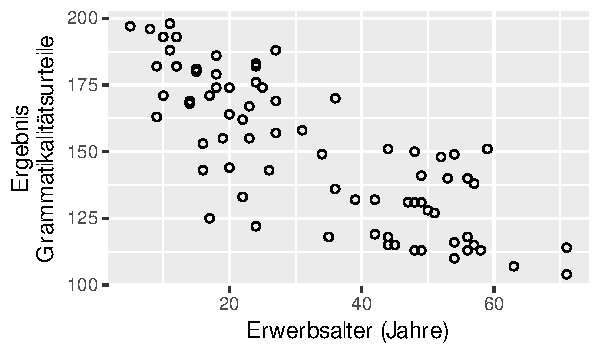
\includegraphics[width=.7\textwidth]{figs/unnamed-chunk-177-1} 

}

\caption{Zusammenhang zwischen AOA und GJT in der Studie von \citet{DeKeyser2010}. Die AOA-Werte stehen entlang der x-Achse und die GJT-Werte entlang der y-Achse, da es plausibler ist, dass das Erwerbsalter die Grammatikalitätsurteile beeinflusst als umgekehrt.\label{fig:dekeyser}}\label{fig:unnamed-chunk-177}
\end{figure}

\end{knitrout}

Das Streudiagramm zeigt, dass die Leistung beim
GJT mit steigendem Erwerbsalter allmählich abnimmt.
Diese Senkung scheint auch ungefähr linear zu sein;
zum Vergleich zeigt Abbildung \ref{fig:nichtlinear} vier
deutliche Beispiele von nicht-linearen Zusammenhängen.
Ausserdem gibt es keine einzelnen
Punkte, die sehr weit von der Punktwolke entfernt liegen,
und alle Daten sind plausibel: Es gibt keine 207-Jährigen
und in \citet{DeKeyser2010} kann man lesen, dass
das GJT-Instrument aus 204 binären Items bestand.
Das höchstmögliche Ergebnis von 204 wird hier nicht überschritten.

\begin{knitrout}
\definecolor{shadecolor}{rgb}{0.969, 0.969, 0.969}\color{fgcolor}\begin{figure}[tp]

{\centering 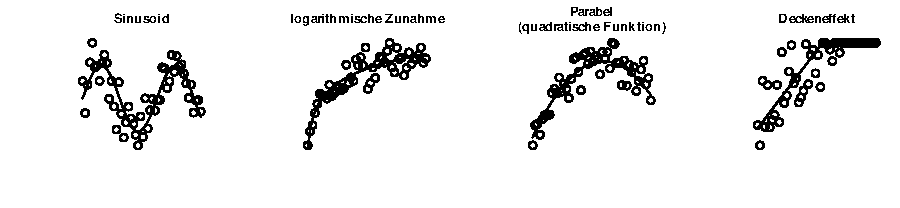
\includegraphics[width=\textwidth]{figs/unnamed-chunk-178-1} 

}

\caption{Beispiele von nicht-linearen Zusammenhängen.\label{fig:nichtlinear}}\label{fig:unnamed-chunk-178}
\end{figure}

\end{knitrout}

\section{Zwei Fragen}

Im Folgenden werden wir eine Antwort auf diese beiden Fragen geben:
\begin{enumerate}
 \item \emph{Wie perfekt} ist der Zusammenhang zwischen den GJT- und AOA-Variablen?
 Wie genau `perfekt' in diesem Kontext zu verstehen ist, sollte in Kürze klar werden.
 Um diese Frage zu beantworten, verwendet man oft \textbf{Korrelationsanalyse}.

 \item \emph{Was} ist der Zusammenhang zwischen den beiden Variablen?
 Anders gesagt, wenn wir den Wert einer Variablen kennen,
 \emph{wie} können wir dann den Wert der anderen Variablen schätzen?
 (\textbf{Regressionsanalyse})
\end{enumerate}

Beide Fragen werden oft miteinander verwechselt, was manchmal zu
Verwirrungen führt \citep[siehe][]{Vanhove2013}. Zwei Beispiele, um den
Unterschied klar zu machen:
\begin{itemize}
 \item Wenn man die Temperatur in Grad Celsius kennt, kann man die Temperatur in Grad Fahrenheit perfekt `schätzen':
 Die Korrelation ist also äusserst stark (Frage 1). Damit wissen wir aber noch nicht, wie wir die Temperatur in Grad Fahrenheit berechnen können, wenn wir die Temperatur in Grad Celsius kennen. Eine Regressionsanalyse würde zeigen, dass wir dazu die folgende Formel anwenden müssten:
\begin{equation}\label{eq:fahrenheit}
 \textrm{Grad Fahrenheit} = 32 + \frac{9}{5} \cdot \textrm{Grad Celsius}.
\end{equation}
\item Wenn man die Körpergrösse eines Menschen kennt, kann man
sein Gewicht wesentlich besser schätzen, als wenn man die
Körpergrösse nicht kennt. Die Schätzung ist aber nicht perfekt,
denn Menschen mit der gleichen Körpergrösse variieren ja in ihrem Gewicht.
Die Korrelation ist folglich zwar positiv, aber nicht so hoch wie im letzten
Beispiel (Frage 1). Um zu wissen, wie man das Gewicht am besten
anhand der Grösse schätzt (z.B.\ $\textrm{Gewicht in kg} = 0.6 \cdot \textrm{Grösse in cm} - 40 \textrm{~kg}$ für Frauen zwischen 145 und 185 cm), braucht es Regressionsanalyse.
\end{itemize}

Die zweite Frage ist m.E.\ in der Regel (nicht immer!) viel sinnvoller.
In unserem Beispiel wäre das Ziel also, eine Gleichung
wie Gleichung \ref{eq:fahrenheit} zu finden, anhand derer
man Unterschiede im GJT-Ergebnis mit Unterschieden
im AOA verknüpfen kann. Um diese Gleichung zu finden,
brauchen wir zuerst aber eine Antwort auf die erste Frage.

\paragraph{Nicht-lineare Zusammenhänge.}
Korrelation- und Regressionsanalyse
können sinnvoll sein, um lineare Zusammenhänge zu
untersuchen. Ist der Zusammenhang zwischen
den Variablen nicht \emph{ungefähr} gerade, dann kann
man die Berechnung noch immer ausführen.
Diese würde dann aber sinnlose (nicht `falsche'!) Ergebnisse liefern.
Bei einem verantwortungsvollen Umgang mit quantitativen Forschungsdaten
sollte die Frage der \textbf{Relevanz} immer im Vordergrund stehen.

Manchmal kann man übrigens
Daten sinnvoll transformieren, sodass der Zusammenhang
linear wird (Beispiele in etwa \citealp{Baayen2008} und \citealp{Gelman2007}).
Ist dies nicht möglich, dann dürften komplexere Verfahren
geeignet sein. Siehe hierzu \citet{Clark2018}, \citet{Wieling2018} und \citet{Baayen2020}.

\medskip

\begin{framed}
\noindent \textbf{Empfehlung: Fragen und Werkzeuge.}
Korrelations-, Regressions- und sonstige Analysen,
Modelle und Tests sind lediglich Werkzeuge. Je nach
Fragestellung sind diese Werkzeuge nützlich oder nutzlos.
Anstatt sich etwa vorzunehmen, eine Korrelationsanalyse
oder einen $t$-Test durchzuführen (vielleicht, weil dies
in einer bestimmten Forschungsliteratur gang und gäbe ist),
ist es sinnvoller, die Frage ohne ablenkenden
technischen Wortschatz (z.B.\ 
\textit{Korrelation}, \textit{signifikant}, \textit{Interaktion})
zu formulieren und sich dann zu überlegen, welches Werkzeug
für deren Beantwortung am nützlichsten ist.
Das Ziel einer Datenerhebung und einer Analyse ist es,
eine Frage zu beantworten, nicht ein bestimmtes Werkzeug zu benutzen.
\end{framed}

\section{Antwort auf Frage 1: Kovarianz und Korrelation}

\subsection{Kovarianz}
Um numerisch zu beschreiben, wie stark zwei Variablen
miteinander zusammenhängen, brauchen wir ein Mass,
dessen absoluter Wert gross ist, wenn kleine Unterschiede
in $x$ mit kleinen Unterschieden in $y$ zusammenhängen
und grosse Unterschiede in $x$ mit grossen Unterschieden
in $y$, und dessen absoluter Wert klein ist, wenn grosse
Unterschiede in der einen Variablen mit nur kleinen Unterschieden
in der anderen Variablen zusammenhängen. Ein solches Mass
ist die Kovarianz:
\begin{equation}\label{eq:covariance}
\textrm{Cov}(x, y) = \frac{1}{n-1} \sum_{i = 1}^{n} (\bar{x} - x_i)(\bar{y}-y_i).
\end{equation}

Die Summe der Produkte ($\sum(\bar{x} - x_i)(\bar{y}-y_i)$) wird durch
$n-1$ statt durch $n$ geteilt aus dem gleichen Grund, weshalb
dies bei der Varianzberechnung gemacht wird. Eine intuitivere
Erklärung ist, dass man ja nicht über den Zusammenhang von zwei
Variablen sprechen kann, wenn man nur eine Beobachtung pro Variable
hat. Das Streudiagramm würde dann nur einen Punkt zeigen.
Wenn $n = 1$, ist $n-1=0$ und dann ergibt die Gleichung keine Antwort,
denn durch 0 kann nicht geteilt werden.

In R:
\begin{knitrout}
\definecolor{shadecolor}{rgb}{0.969, 0.969, 0.969}\color{fgcolor}\begin{kframe}
\begin{alltt}
\hlstd{> }\hlcom{# kompliziert:}
\hlstd{> }\hlkwd{sum}\hlstd{((}\hlkwd{mean}\hlstd{(d}\hlopt{$}\hlstd{AOA)} \hlopt{-} \hlstd{d}\hlopt{$}\hlstd{AOA)} \hlopt{*} \hlstd{(}\hlkwd{mean}\hlstd{(d}\hlopt{$}\hlstd{GJT)} \hlopt{-} \hlstd{d}\hlopt{$}\hlstd{GJT))} \hlopt{/} \hlstd{(}\hlkwd{nrow}\hlstd{(d)} \hlopt{-} \hlnum{1}\hlstd{)}
\end{alltt}
\begin{verbatim}
[1] -394.9311
\end{verbatim}
\begin{alltt}
\hlstd{> }\hlcom{# einfacher:}
\hlstd{> }\hlkwd{cov}\hlstd{(d}\hlopt{$}\hlstd{AOA, d}\hlopt{$}\hlstd{GJT)}
\end{alltt}
\begin{verbatim}
[1] -394.9311
\end{verbatim}
\end{kframe}
\end{knitrout}

Ist die Kovarianz positiv, dann besteht ein
positiver linearer Zusammenhang zwischen den beiden
Variablen (je grösser $x$, desto grösser $y$);
ist die Kovarianz negativ, dann gibt es einen negativen linearen
Zusammenhang (je grösser $x$, desto kleiner $y$).
Abgesehen von diesen zwei Richtschnuren ist das
Kovarianzmass schwierig zu interpretieren, weshalb
Sie es in der Literatur nur selten antreffen
werden. Aber Kovarianz ist ein wichtiges Konzept in der
Mathe hinter komplexeren Verfahren,
weshalb es sich trotzdem lohnt, zumindest zu wissen,
dass es besteht.

\paragraph{Aufgabe 1.} Seien $x$ und $y$ zwei numerische Variablen.
Macht es etwas aus, ob man
$\textrm{Cov}(x,y)$ oder $\textrm{Cov}(y,x)$ berechnet? Beantworten Sie diese Frage,
indem Sie sich Formel \ref{eq:covariance} genauer anschauen.

\paragraph{Aufgabe 2.} Was ist die Kovarianz zwischen $x$ und $y$, wenn
es zwar unterschiedliche $x$-Werte gibt, aber alle $y$-Werte einander gleich sind?
Beantworten Sie diese Frage,
indem Sie sich Formel \ref{eq:covariance} genauer anschauen.

\paragraph{Aufgabe 3.} Sei $x$ eine numerische Variable. Was berechnen Sie
eigentlich genau, wenn Sie $\textrm{Cov}(x,x)$ berechnen?
Beantworten Sie diese Frage,
indem Sie sich Formel \ref{eq:covariance} genauer anschauen.

\subsection{Korrelation}
Da das Kovarianzmass nicht einfach zu interpretieren ist,
wird meistens Pearsons \textbf{Produkt-Moment-Korrelationskoeffizient}
($r$) (oder einfach Pearsons Korrelation) verwendet.
Diese Zahl drückt aus, wie gut der Zusammenhang durch eine gerade Linie
beschrieben werden kann. Es wird ähnlich zum Kovarianzmass
berechnet, aber die Variablen werden in Standardabweichungen zum
Stichprobemittel ausgedrückt. Dies ergibt dann immer eine Zahl
zwischen $-1$ und $1$:
\[
r_{xy} = \frac{1}{n-1} \sum_{i = 1}^{n} \frac{\bar{x} - x_i}{s_x} \frac{\bar{y}-y_i}{s_y} = \frac{\textrm{Cov}(x, y)}{s_x s_y}.
\]
\begin{knitrout}
\definecolor{shadecolor}{rgb}{0.969, 0.969, 0.969}\color{fgcolor}\begin{kframe}
\begin{alltt}
\hlstd{> }\hlcom{# kompliziert:}
\hlstd{> }\hlkwd{cov}\hlstd{(d}\hlopt{$}\hlstd{AOA, d}\hlopt{$}\hlstd{GJT)} \hlopt{/} \hlstd{(}\hlkwd{sd}\hlstd{(d}\hlopt{$}\hlstd{AOA)} \hlopt{*} \hlkwd{sd}\hlstd{(d}\hlopt{$}\hlstd{GJT))}
\end{alltt}
\begin{verbatim}
[1] -0.8028533
\end{verbatim}
\begin{alltt}
\hlstd{> }\hlcom{# einfach:}
\hlstd{> }\hlkwd{cor}\hlstd{(d}\hlopt{$}\hlstd{AOA, d}\hlopt{$}\hlstd{GJT)}
\end{alltt}
\begin{verbatim}
[1] -0.8028533
\end{verbatim}
\end{kframe}
\end{knitrout}

Sobald irgendein Wert fehlt, ergibt die \texttt{cor()}-Funktion
das Ergebnis `NA` (\textit{not available}). Eine Möglichkeit
ist dann, die Beobachtungen mit einem oder zwei fehlenden Werten zu ignorieren:
\begin{knitrout}
\definecolor{shadecolor}{rgb}{0.969, 0.969, 0.969}\color{fgcolor}\begin{kframe}
\begin{alltt}
\hlstd{> }\hlkwd{cor}\hlstd{(d}\hlopt{$}\hlstd{AOA, d}\hlopt{$}\hlstd{GJT,} \hlkwc{use} \hlstd{=} \hlstr{"pairwise.complete.obs"}\hlstd{)}
\end{alltt}
\begin{verbatim}
[1] -0.8028533
\end{verbatim}
\end{kframe}
\end{knitrout}
Ist $r = 1$, dann liegen alle Datenpunkte perfekt auf einer geraden, steigenden Linie.
Dies deutet fast ausnahmslos auf eine Tautologie hin.
Zum Beispiel sind Körpergrössen in Zentimetern und in Zoll perfekt korreliert,
aber dieser Zusammenhang ist nicht spektakulär sondern höchst langweilig.
Ist $r = -1$, dann liegen alle Datenpunkte auf einer geraden, senkenden Linie.
Dies deutet wohl darauf hin, dass die beiden Variablen perfekt komplementär sind.
Zum Beispiel wird die Anzahl richtiger Antworten bei einem Test oft zu $r = -1$ mit der Anzahl falscher Antworten korrelieren; auch dies ist wenig spektakulär.
Ist $r = 0$, dann ist die Linie perfekt senkrecht, d.h., es gibt überhaupt keinen linearen Zusammenhang zwischen den beiden Variablen.
Je grösser der absolute Wert von $r$, desto näher befinden sich die Datenpunkte bei der geraden Linie.
Anders ausgedrückt: Je grösser der absolute $r$-Wert, desto präziser kann man $y$ bestimmen, wenn man $x$ schon kennt (und umgekehrt) als wenn man $x$
nicht gekannt hätte.
% Die Korrelation zwischen $x$ und $y$ ist gleich der Korrelation zwischen $y$ und $x$.
% Es macht also nichts aus, ob man \texttt{cor(dat\$AOA, dat\$GJT)} oder \texttt{cor(dat\$GJT, dat\$AOA)} eintippt.

Abbildung \ref{fig:correlation} zeigt vier Zusammenhänge,
um die Bedeutung von Pearsons $r$ besser zu illustrieren.
\begin{itemize}
\item \textit{Oben links:} Es gibt wenig Streuung entlang der $y$-Achse.
Die Streuung, die es gibt, wird grösstenteils von einer Geraden erfasst.
$r$ ist daher sehr hoch.
\item \textit{Oben rechts:} Es gibt nun mehr Streuung entlang der $y$-Achse;
diese wird aber weniger gut von einer Geraden erfasst, daher der niedrigere Korrelationskoeffizient.
Die Form der Geraden ist zwar gleich wie in der linken Grafik, der Korrelationskoeffizient aber nicht.
\item \textit{Unten links:} Es gibt zwar sehr viel Streuung entlang der $y$-Achse, aber diese wird grösstenteils von einer Geraden erfasst. $r$ ist daher wiederum sehr hoch. Der Korrelationskoeffizient ist zwar gleich wie in der Grafik oberhalb,
die Form der Geraden aber nicht.
\item \textit{Unten rechts:} Die gleiche Gerade erfasst die Streuung entlang der $y$-Achse weniger gut, daher ist die Form der Geraden zwar gleich, der Korrelationskoeffizient aber niedriger.
\end{itemize}

\begin{knitrout}
\definecolor{shadecolor}{rgb}{0.969, 0.969, 0.969}\color{fgcolor}\begin{figure}[tp]

{\centering 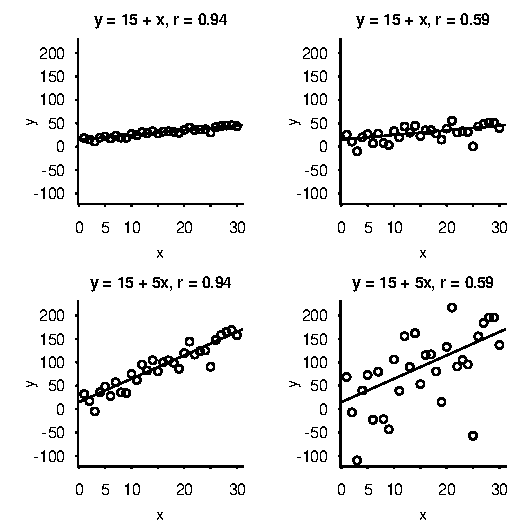
\includegraphics[width=.5\textwidth]{figs/unnamed-chunk-182-1} 

}

\caption{Korrelationskoeffizienten erzählen einem wenig über die Form eines Zusammenhangs.\label{fig:correlation}}\label{fig:unnamed-chunk-182}
\end{figure}

\end{knitrout}
\subsubsection{Welche Frage beantwortet $r$ (und welche nicht)?}
Wie wir gerade gesehen haben, drückt Pearsons $r$ aus,
welcher Anteil der Streuung der Datenpunkte in einer Punktwolke durch
eine \emph{gerade Linie} erfasst wird.
Es gibt keine direkte Antwort auf die Frage, wie diese Linie ausschaut
(ausser: steigend oder senkend);
siehe die vier obigen Beispiele.

Ausserdem ist es möglich, dass es einen sehr starken (nicht-linearen) Zusammenhang zwischen zwei Variablen gibt,
dieser aber in Pearsons $r$ nicht zum Ausdruck kommt (Abbildung \ref{fig:nonlinearcorrelation}, links).
Umgekehrt kann $r$ den Eindruck geben, dass es sich um einen ziemlich starken linearen Zusammenhang handelt, während ein solcher Zusammenhang für die meisten Datenpunkte kaum vorliegt (Mitte),
oder während der Zusammenhang sogar eigentlich in die umgekehrte Richtung geht.
So gibt es in der rechten Grafik zwei Gruppen, in denen der Zusammenhang negativ ist.
Der Koeffizient ist jedoch positiv, wenn die beiden Gruppen gleichzeitig betrachtet werden.
Das Problem ist hier nicht, dass $r$ falsch berechnet wird,
sondern, dass die Berechnung von $r$ hier kaum Sinn ergibt.
Bevor man sich mit der Richtigkeitsfrage auseinandersetzt,
sollte man sich eben zuerst mit der Relevanzfrage befassen.

\begin{knitrout}
\definecolor{shadecolor}{rgb}{0.969, 0.969, 0.969}\color{fgcolor}\begin{figure}[tp]

{\centering 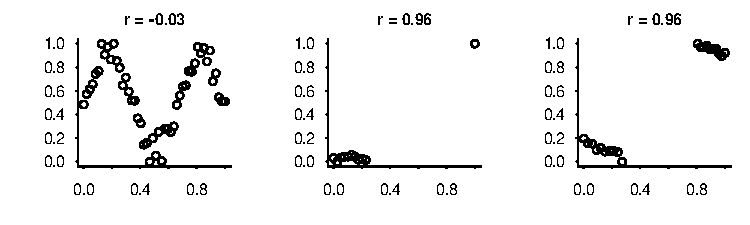
\includegraphics[width=.9\textwidth]{figs/unnamed-chunk-183-1} 

}

\caption{Ein Korrelationskoeffizient nahe 0 muss nicht heissen, dass es keinen Zusammenhang zwischen den Variablen gibt, und ein Korrelationskoeffizient nahe 1 muss nicht heissen, dass das Muster in den Daten am besten durch einen starken positiven Zusammenhang beschrieben wird.\label{fig:nonlinearcorrelation}}\label{fig:unnamed-chunk-183}
\end{figure}

\end{knitrout}

Mit der \texttt{plot\_r()}-Funktion im \texttt{cannonball}-Paket
können Sie selber Streudiagramme zeichnen, die alle anders aussehen,
aber den gleichen Korrelationskoeffizienten haben.
Unter \url{https://github.com/janhove/cannonball} finden Sie
Anweisungen, wie Sie dieses Paket installieren können.
Der Blogeintrag \href{https://janhove.github.io/teaching/2016/11/21/what-correlations-look-like}{\textit{What data patterns can lie behind a correlation coefficient?}} (21.11.2016)
beschreibt die \texttt{plot\_r()}-Funktion.
Abbildung \ref{fig:plotr} zeigt 16 Zusammenhänge mit je 50 Beobachtungen, die
alle eine Korrelation von $r = -0.72$ aufzeigen:
\begin{knitrout}
\definecolor{shadecolor}{rgb}{0.969, 0.969, 0.969}\color{fgcolor}\begin{kframe}
\begin{alltt}
\hlstd{> }\hlkwd{library}\hlstd{(cannonball)}
\hlstd{> }\hlkwd{plot_r}\hlstd{(}\hlkwc{n} \hlstd{=} \hlnum{50}\hlstd{,} \hlkwc{r} \hlstd{=} \hlopt{-}\hlnum{0.72}\hlstd{)}
\end{alltt}
\end{kframe}\begin{figure}[tp]

{\centering 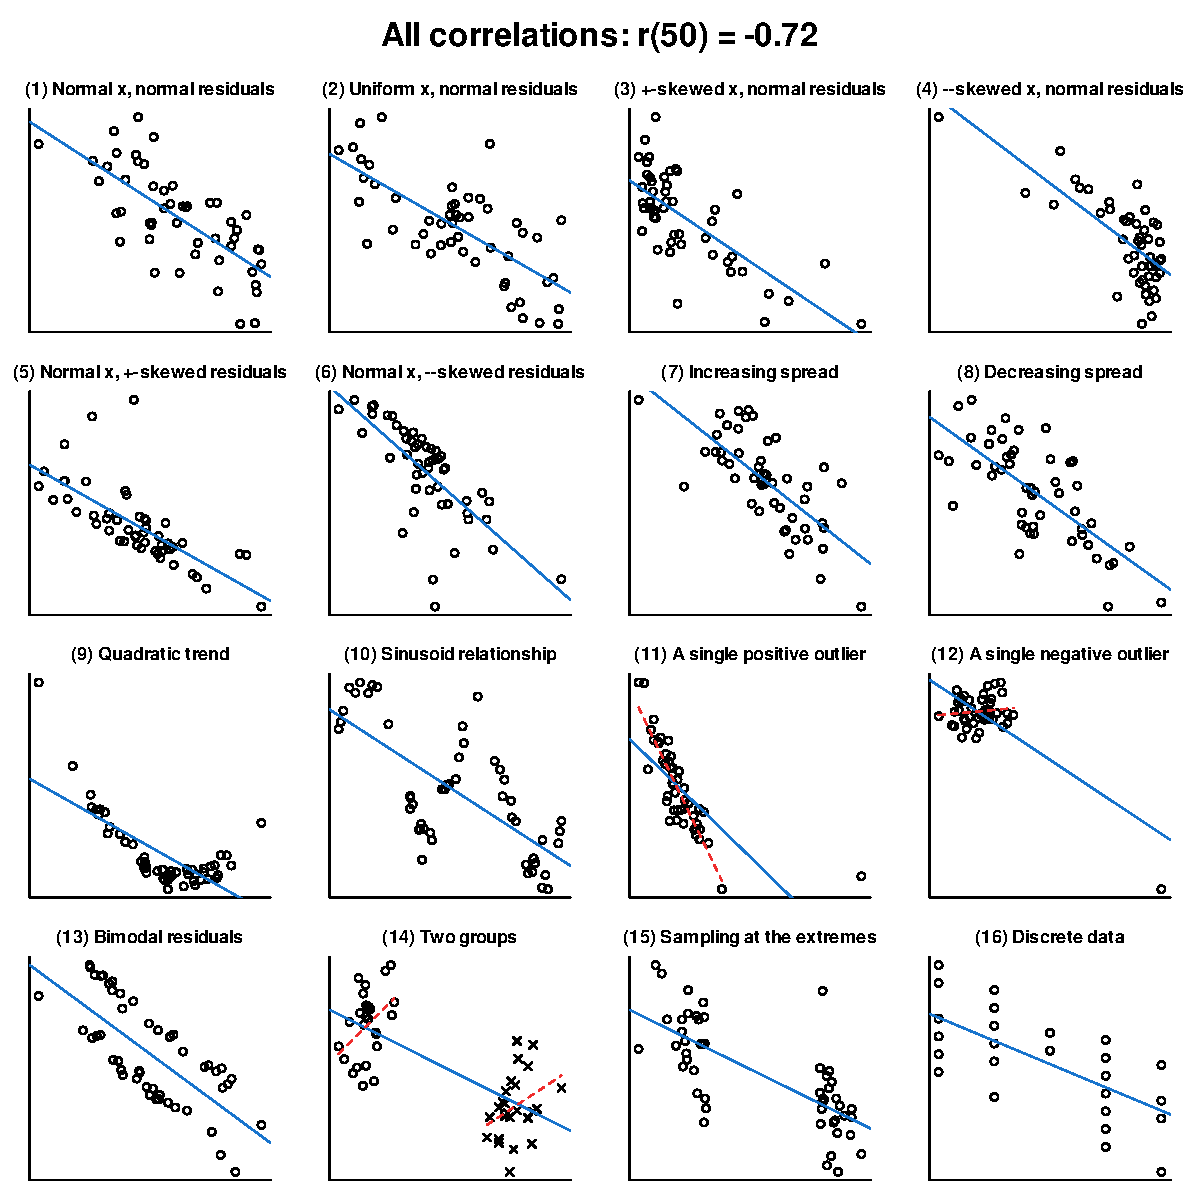
\includegraphics[width=\textwidth]{figs/unnamed-chunk-184-1} 

}

\caption{Alle sechzehn Zusammenhänge zeigen eine Korrelation von $-0.72$ auf, sehen jedoch zum Teil ganz unterschiedlich aus.\label{fig:plotr}}\label{fig:unnamed-chunk-184}
\end{figure}

\end{knitrout}
Spielen Sie mit der \texttt{plot\_r()}-Funktion herum,
um besser zu verstehen, was ein Korrelationskoeffizient eben alles nicht bedeutet
und was der Einfluss von nicht-linearen Zusammenhängen und Ausreissern sein kann:
\begin{knitrout}
\definecolor{shadecolor}{rgb}{0.969, 0.969, 0.969}\color{fgcolor}\begin{kframe}
\begin{alltt}
\hlstd{> }\hlkwd{plot_r}\hlstd{(}\hlkwc{n} \hlstd{=} \hlnum{15}\hlstd{,} \hlkwc{r} \hlstd{=} \hlnum{0.9}\hlstd{)}
\hlstd{> }\hlkwd{plot_r}\hlstd{(}\hlkwc{n} \hlstd{=} \hlnum{80}\hlstd{,} \hlkwc{r} \hlstd{=} \hlnum{0.0}\hlstd{)}
\hlstd{> }\hlkwd{plot_r}\hlstd{(}\hlkwc{n} \hlstd{=} \hlnum{30}\hlstd{,} \hlkwc{r} \hlstd{=} \hlnum{0.4}\hlstd{)}
\end{alltt}
\end{kframe}
\end{knitrout}
Die Funktionsdokumentation können Sie wie gehabt abrufen:
\begin{knitrout}
\definecolor{shadecolor}{rgb}{0.969, 0.969, 0.969}\color{fgcolor}\begin{kframe}
\begin{alltt}
\hlstd{> }\hlopt{?}\hlstd{plot_r}
\end{alltt}
\end{kframe}
\end{knitrout}


\medskip

\begin{framed}
\noindent \textbf{Merksatz: Ein Korrelationskoeffizient kann einer Vielzahl von Zusammenhängen entsprechen.}
Schauen Sie sich, bevor Sie Korrelationskoeffizienten berechnen, immer die Daten \textbf{grafisch}
(Streudiagramm) an.
Nehmen Sie diese Streudiagramme in Ihre Papers, Arbeiten und Vorträge auf.
Ein Korrelationskoeffizient ohne Streudiagramm ist m.E.\ wertlos.
\end{framed}

\subsubsection{Andere Korrelationsmasse}
Ab und zu trifft man in der Forschungsliteratur
Spearmans $\rho$-Koeffizienten (oder manchmal: $r_s$) an.
Hierfür drückt man die Daten in \textbf{Rängen} aus,
d.h., man ordnet die Daten von klein nach gross und schaut,
auf welchem Platz die einzelnen Datenpunkte stehen.
Der Datenpunkt auf Rang 1 ist übrigens der niedrigste Datenpunkt,
das heisst, die Reihenfolge der ursprünglichen Werte wird behalten und nicht umgedreht.
Dann berechnet man einfach die Pearsonkorrelation für die Ränge statt für die Rohwerte:
\begin{knitrout}
\definecolor{shadecolor}{rgb}{0.969, 0.969, 0.969}\color{fgcolor}\begin{kframe}
\begin{alltt}
\hlstd{> }\hlkwd{cor}\hlstd{(}\hlkwd{rank}\hlstd{(d}\hlopt{$}\hlstd{AOA),} \hlkwd{rank}\hlstd{(d}\hlopt{$}\hlstd{GJT))}
\end{alltt}
\begin{verbatim}
[1] -0.7887659
\end{verbatim}
\begin{alltt}
\hlstd{> }\hlcom{# einfacher:}
\hlstd{> }\hlkwd{cor}\hlstd{(d}\hlopt{$}\hlstd{AOA, d}\hlopt{$}\hlstd{GJT,} \hlkwc{method} \hlstd{=} \hlstr{"spearman"}\hlstd{)}
\end{alltt}
\begin{verbatim}
[1] -0.7887659
\end{verbatim}
\end{kframe}
\end{knitrout}

Spearmans $\rho$ kann nützlich sein, wenn der Zusammenhang zwischen zwei Variablen monoton aber nicht-linear ist (Monoton heisst: Tendenziell steigend oder tendenziell senkend; nicht etwa zuerst steigend und dann senkend.) oder wenn ein \textbf{Ausreisser} das Globalbild zerstört, aber man ihn aus irgendwelchem Grund nicht aus dem Datensatz entfernen kann.
Wenn Spearmans $\rho = 1$, dann ist der Zusammenhang perfekt monoton steigend (höhere Werte
in $x$ entsprechen immer höheren Werten in $y$),
wenn Spearmans $\rho = -1$, dann ist der Zusammenhang perfekt monoton senkend,
und wenn $\rho = 0$, dann gibt es keinen monotonen Zusammenhang in den Daten.
Bemerken Sie, dass man mit $\rho$ eine andere Frage beantwortet als mit $r$:
\textit{Wie perfekt ist der monotone Zusammenhang?} vs. \textit{Wie perfekt ist der lineare Zusammenhang?}

Ein anderes Mass ist Kendalls $\tau$ (\texttt{method = "kendall"}).
Dieses wird aber nur höchst selten verwendet. Die Berechnung ist
konzeptuell relativ einfach \citep[siehe][]{Noether1981}, aber schaut in R-Code schwierig aus,
weshalb ich sie hier nur in Worten zusammenfasse:

\begin{enumerate}
 \item Vergleiche jeden $x$-Wert mit jedem anderen $x$-Wert und
 notiere, ob Ersterer grösser oder kleiner als Letzterer ist.
 Wenn die $x$-Werte zum Beispiel 5, 3, 8 und 7 sind,
 erhält man folgende Vergleiche:
 \begin{itemize}
  \item 5 vs.\ 3: grösser,
  \item 5 vs.\ 8: kleiner,
  \item 5 vs.\ 7: kleiner,
  \item 3 vs.\ 8: kleiner,
  \item 3 vs.\ 7: kleiner,
  \item 8 vs.\ 7: grösser.
 \end{itemize}
 \item Vergleiche jeden $y$-Wert mit jedem anderen $y$-Wert.
 Für die $y$-Werte 8, $-2$, $-4$, $-3$ erhält man:
 grösser, grösser, grösser, grösser, grösser, kleiner.
 \item Zähle, wie viele Vergleiche in die gleiche
 Richtung gehen:
 \begin{itemize}
  \item 1.~Vergleich: grösser--grösser: gleich,
  \item 2.~Vergleich: kleiner--grösser: anders,
  \item 3.~Vergleich: kleiner--grösser: anders,
  \item 4.~Vergleich: kleiner--grösser: anders,
  \item 5.~Vergleich: kleiner--grösser: anders,
  \item 6.~Vergleich: grösser--kleiner: anders.
 \end{itemize}
 Also 1 Vergleich, der in die gleiche Richtung geht (`konkordant'),
 und 5, die in die andere Richtung gehen (`diskordant').
 \item Schätze jetzt Kendalls $\tau$ wie folgt:
 \begin{equation*}
 \hat{\tau} = \frac{\textrm{Anzahl konkordant} - \textrm{Anzahl diskordant}}{\textrm{Anzahl Vergleiche}}.
 \end{equation*}
 Das Hütchen zeigt, dass wir es mit einer Schätzung auf der Basis
 einer Stichprobe zu tun haben.
 Also:
  \begin{equation*}
 \hat{\tau} = \frac{1 - 5}{6} = -0.67.
 \end{equation*}
\end{enumerate}

\begin{knitrout}
\definecolor{shadecolor}{rgb}{0.969, 0.969, 0.969}\color{fgcolor}\begin{kframe}
\begin{alltt}
\hlstd{> }\hlcom{# Für unser kleines Beispiel}
\hlstd{> }\hlstd{x} \hlkwb{<-} \hlkwd{c}\hlstd{(}\hlnum{5}\hlstd{,} \hlnum{3}\hlstd{,} \hlnum{8}\hlstd{,} \hlnum{7}\hlstd{)}
\hlstd{> }\hlstd{y} \hlkwb{<-} \hlkwd{c}\hlstd{(}\hlnum{8}\hlstd{,} \hlopt{-}\hlnum{2}\hlstd{,} \hlopt{-}\hlnum{4}\hlstd{,} \hlopt{-}\hlnum{3}\hlstd{)}
\hlstd{> }\hlkwd{cor}\hlstd{(x, y,} \hlkwc{method} \hlstd{=} \hlstr{"kendall"}\hlstd{)}
\end{alltt}
\begin{verbatim}
[1] -0.6666667
\end{verbatim}
\begin{alltt}
\hlstd{> }\hlcom{# Für die AOA-GJT-Daten}
\hlstd{> }\hlkwd{cor}\hlstd{(d}\hlopt{$}\hlstd{AOA, d}\hlopt{$}\hlstd{GJT,} \hlkwc{method} \hlstd{=} \hlstr{"kendall"}\hlstd{)}
\end{alltt}
\begin{verbatim}
[1] -0.6035606
\end{verbatim}
\end{kframe}
\end{knitrout}

Kendalls $\hat{\tau}$ schätzt den Unterschied zwischen
der Proportion konkordanter Vergleiche und der Proportion
diskordanter Vergleiche. Diese Interpretation finde ich
selber schwierig, aber es gibt eine einfachere Interpretation:
Nimm zwei beliebige $(x, y)$-Paare (also ($x_1, y_1$) und ($x_2, y_2$)).
Wenn $x_2$ grösser ist als $x_1$, dann ist es $\frac{1 + \hat{\tau}}{1 - \hat{\tau}}$
Mal wahrscheinlicher, dass auch $y_2$ grösser als $y_1$ ist als dass er kleiner ist.
Für die AOA--GJT-Daten: Wenn eine Person einen höheren AOA-Wert als
eine andere hat, dann ist es $\frac{1+(-0.60)}{1-(-0.60)} = 0.25$ Mal
wahrscheinlicher, dass sie auch einen höheren GJT-Wert als einen kleineren hat.
Oder anders gesagt: Es ist 4 Mal wahrscheinlicher, dass sie einen kleineren GJT-Wert
als einen grösseren hat.

In der Praxis ist die Anwendung von Spearmans $\rho$ und Kendalls
$\tau$ ist eher beschränkt.
Statt automatisch auf $\rho$ oder $\tau$ zurückzugreifen,
wenn ein Zusammenhang nicht-linear ist
oder wenn man einen Ausreisser vermutet,
lohnt es sich m.E.\ eher, darüber nachzudenken,
ob (a) man sich tatsächlich für Frage 1
(Stärke des Zusammenhangs) interessiert (die Relevanzfrage),
(b) man eine oder beide Variablen nicht
sinnvoll transformieren kann, sodass
sich ein linearerer Zusammenhang ergibt,
oder (c) der vermutete Ausreisser
überhaupt ein legitimer Datenpunkt ist.

\subsubsection{Starke und schwache Korrelationen}
Korrelationskoeffizienten werden oft---ohne
Berücksichtigung der Forschungsfrage oder des
Kontextes---als klein, mittelgross oder gross
eingestuft. Ich halte dies für wenig sinnvoll,
weshalb ich diese Einstufungen hier nicht
reproduziere.
% Wer mehr über sie erfahren möchte,
% kann sich bei \citet{Cohen1992} und \citet{Plonsky2014}
% selber schlau machen. Dazu empfiehlt sich auch
% die Lektüre von \citet{Baguley2009}.
Selber finde ich, dass
Korrelationskoeffizienten überverwendet werden.
Blogeinträge zu diesem Thema:
\begin{itemize}
\item \href{https://janhove.github.io/reporting/2015/02/05/standardised-vs-unstandardised-es}{\textit{Why I don't like standardised effect sizes}} (5.2.2015)
\item \href{https://janhove.github.io/design/2015/03/16/standardised-es-revisited}{\textit{More on why I don't like standardised effect sizes}} (16.3.2015)
\item \href{https://janhove.github.io/design/2017/07/14/OtherRoadsToPower}{\textit{Abandoning standardised effect sizes and opening up other roads to power}} (14.7.2017)
\end{itemize}
Siehe weiter auch \citet{Baguley2009}.

\subsection{Die Ungenauigkeit eines Korrelationskoeffizienten einschätzen}
Da sie auf der Basis von Stichproben berechnet werden,
sind auch Korrelationskoeffizienten vom Stichprobenfehler betroffen:
Andere Stichproben aus der gleichen Population werden Korrelationskoeffizienten
ergeben, die mehr oder weniger voneinander abweichen.
Die Ungenauigkeit bzw.\ die Variabilität eines auf einer Stichprobe
basierenden Korrelationskoeffizienten kann in einem Konfidenzintervall
ausgedrückt werden. Besprochen werden hier eine Bootstrap-Methode
und eine Methode, die auf $t$-Verteilungen basiert.

\paragraph{Mit dem Bootstrap.}\label{sec:r_bootstrap}
Das Vorgehen ist analog zum Bootstrap aus Kapitel \ref{ch:uncertainty}:
Aus der Stichprobe
werden neue Bootstrap-Stichproben generiert und für jede Stichprobe
wird die Statistik von Interesse (hier: die Korrelation zwischen AOA und GJT)
berechnet. Die Streuung der Schätzungen in den Bootstrap-Stichproben
gibt uns ein Indiz über die Variabilität des Korrelationskoeffizienten
in Stichproben dieser Grösse.
\begin{knitrout}
\definecolor{shadecolor}{rgb}{0.969, 0.969, 0.969}\color{fgcolor}\begin{kframe}
\begin{alltt}
\hlstd{> }\hlstd{n_bootstraps} \hlkwb{<-} \hlnum{20000}
\hlstd{> }\hlstd{bootstraps} \hlkwb{<-} \hlkwd{vector}\hlstd{(}\hlkwc{length} \hlstd{= n_bootstraps)}
\hlstd{> }
\hlstd{> }\hlkwa{for} \hlstd{(i} \hlkwa{in} \hlnum{1}\hlopt{:}\hlstd{n_bootstraps) \{}
\hlstd{+ }  \hlcom{# Sampling with replacement aus der beobachteten Stichprobe}
\hlstd{+ }  \hlstd{bootstrap_sample} \hlkwb{<-} \hlstd{d |>}
\hlstd{+ }    \hlkwd{slice_sample}\hlstd{(}\hlkwc{prop} \hlstd{=} \hlnum{1}\hlstd{,} \hlkwc{replace} \hlstd{=} \hlnum{TRUE}\hlstd{)}

\hlstd{+ }  \hlcom{# Korrelation im bootstrap sample berechnen und speichern}
\hlstd{+ }  \hlstd{bootstraps[[i]]} \hlkwb{<-} \hlkwd{cor}\hlstd{(bootstrap_sample}\hlopt{$}\hlstd{GJT, bootstrap_sample}\hlopt{$}\hlstd{AOA)}
\hlstd{+ }\hlstd{\}}
\end{alltt}
\end{kframe}
\end{knitrout}

\begin{knitrout}
\definecolor{shadecolor}{rgb}{0.969, 0.969, 0.969}\color{fgcolor}\begin{kframe}
\begin{alltt}
\hlstd{> }\hlcom{# Histogramm mit den Bootstrap-Schätzungen}
\hlstd{> }\hlcom{# (nicht gezeigt)}
\hlstd{> }\hlkwd{hist}\hlstd{(bootstraps,} \hlkwc{breaks} \hlstd{=} \hlnum{20}\hlstd{)}
\end{alltt}
\end{kframe}
\end{knitrout}

Da das Histogramm nicht normalverteilt ist, verzichten
wir hier auf die Berechnung eines Standardfehlers.
% (Die Verteilung von Stichproben-Korrelationskoeffizienten
% kann nicht normalverteilt sein, da Korrelationskoeffizienten
% zwischen $-1$ und $1$ begrenzt sind.)
Anhand der Perzentile der Verteilung können wir aber durchaus
ein Konfidenzintervall konstruieren. Hier berechne ich
ein 90\%-Konfidenzintervall:
\begin{knitrout}
\definecolor{shadecolor}{rgb}{0.969, 0.969, 0.969}\color{fgcolor}\begin{kframe}
\begin{alltt}
\hlstd{> }\hlkwd{quantile}\hlstd{(bootstraps,} \hlkwc{probs} \hlstd{=} \hlkwd{c}\hlstd{(}\hlnum{0.05}\hlstd{,} \hlnum{0.95}\hlstd{))}
\end{alltt}
\begin{verbatim}
        5%        95% 
-0.8648265 -0.7291892 
\end{verbatim}
\end{kframe}
\end{knitrout}

\medskip
\begin{framed}
\noindent \textbf{Einschub: 80, 90, 95?}
Mittlerweile fragen Sie sich vielleicht, wieso wir
mal ein 80\%-Konfidenzintervall berechnen,
mal ein 90\%-Konfidenzintervall und mal ein
95\%-Konfidenzintervall. Das ist lediglich mein
Versuch, Ihnen zu zeigen, dass die übliche Wahl von
95\% recht arbiträr ist. Zum gleichen Zweck
berechnet \citet{McElreath2020} immer 89\%-Intervalle!
\end{framed}

\paragraph{Mit $t$-Verteilungen.}
Die Formel, mit der man anhand von einer $t$-Verteilung
ein Konfidenzintervall um einen Korrelationskoeffizienten
konstruiert, werde ich hier nicht reproduzieren, da sie
erstens abschreckt und zweitens keinen konzeptuellen
Mehrwert bietet. Sie basiert auf der Annahme, dass
die Population, aus der die beiden Variablen gezogen wurden,
`bivariat normal' ist. Grundsätzlich heisst dies, dass---insofern
es einen Zusammenhang zwischen den Variablen gibt---dieser Zusammenhang
linear ist und beide Variablen normalverteilt sind.
Wenn diese Annahmen plausibel sind,
kann das Konfidenzinterval (hier wiederum ein 90\%-Konfidenzintervall)
mit der \texttt{cor.test()}-Funktion berechnet werden:
\begin{knitrout}
\definecolor{shadecolor}{rgb}{0.969, 0.969, 0.969}\color{fgcolor}\begin{kframe}
\begin{alltt}
\hlstd{> }\hlkwd{cor.test}\hlstd{(d}\hlopt{$}\hlstd{AOA, d}\hlopt{$}\hlstd{GJT,} \hlkwc{conf.level} \hlstd{=} \hlnum{0.9}\hlstd{)}
\end{alltt}
\begin{verbatim}

	Pearson's product-moment correlation

data:  d$AOA and d$GJT
t = -11.584, df = 74, p-value < 2.2e-16
alternative hypothesis: true correlation is not equal to 0
90 percent confidence interval:
 -0.8614924 -0.7230816
sample estimates:
       cor 
-0.8028533 
\end{verbatim}
\end{kframe}
\end{knitrout}

Mit dieser Methode erhalten wir ein 90\%-Konfidenzintervall
von $[-0.86, -0.72]$. Dieses unterscheidet sich nur minimal
vom Konfidenzintervall, das wir mit dem Bootstrap berechnet haben.
Beim Bootstrap sind wir jedoch nicht davon ausgegangen, dass
die Population, aus der die Stichprobe stammt, bivariat normalverteilt war.
Insbesondere bei kleineren Stichproben können die Ergebnisse
der Bootstrap- und der $t$-Methode erheblich voneinander abweichen.
Wenn ihre Annahmen stimmen, ist die $t$-Methode in solchen Fällen zweifellos
besser, aber gerade bei kleinen Stichproben sind diese Annahmen schwierig
zu überprüfen.
Die Leistung der Bootstrapmethode kann noch etwas verbessert
werden, indem die Konfidenzintervalle anders konstruiert werden
\citep[siehe hierzu][]{DiCiccio1996}, aber diese Konstruktionsmethoden
sind schwieriger und weniger intuitiv.
Für unsere Zwecke reicht es
m.E., die Warnung von \citet{Hesterberg2015} zu wiederholen:
``Bootstrapping does not overcome the weakness of small samples
as a basis for inference.'' (S. 379)

Was `$t = -11.6$' und '$\textrm{p-value} < 2.2\textrm{e}-16$' heissen,
werden wir in einem späteren Kapitel besprechen.

\paragraph{Konfidenzintervalle um Korrelationskoeffizienten rekonstruieren?}
Das Konfidenzintervall um einen Korrelationskoeffizienten
hängt von nur drei Faktoren ab:
\begin{itemize}
 \item ob das Konfidenzintervall ein 50\%-, 80\%-, 87\%- usw.-Konfidenzintervall sein soll;
 \item dem Korrelationskoeffizienten selber;
 \item der Anzahl beobachteter Paare.
\end{itemize}
Wenn man weiss, was der Korrelationskoeffizient ist, und wie gross die Stichprobe
war, kann man also selber das Konfidenzintervall berechnen.
Selber finde ich dies nützlich, wenn das Konfidenzintervall um $r$ in
einer Studie nicht berichtet wurde. Mit der Funktion \texttt{r.test()}
aus dem \texttt{psych}-Package ist dies ein Kinderspiel, allerdings
werden nur 95\%-Konfidenzintervalle berechnet.
Gegebenenfalls müssen Sie das \texttt{psych}-Paket noch installieren.
\begin{knitrout}
\definecolor{shadecolor}{rgb}{0.969, 0.969, 0.969}\color{fgcolor}\begin{kframe}
\begin{alltt}
\hlstd{> }\hlstd{psych}\hlopt{::}\hlkwd{r.test}\hlstd{(}\hlkwc{r12} \hlstd{=} \hlopt{-}\hlnum{0.80}\hlstd{,} \hlkwc{n} \hlstd{=} \hlnum{76}\hlstd{)}
\end{alltt}
\begin{verbatim}
Correlation tests 
Call:psych::r.test(n = 76, r12 = -0.8)
Test of significance of a  correlation 
 t value -11.47    with probability < 0
 and confidence interval  -0.87 -0.7
\end{verbatim}
\end{kframe}
\end{knitrout}
Übrigens: Mit der Notation \texttt{psych::r.test()} brauchen Sie das
\texttt{psych}-Package nicht mit dem Befehl \texttt{library(psych)} zu laden.
Dies ist nützlich, wenn man aus einem Paket eh nur eine Funktion
braucht.

Das 95\%-Konfidenzintervall eines Korrelationskoeffizienten
von $r = -0.80$ in einer Stichprobe mit 76 Datenpunkten ist also
$[-0.87, -0.70]$. Dabei gehen wir zwar davon aus, dass die Stichprobe
aus einer bivariaten Normalverteilung stammt, aber bei 76 Beobachtungen
würden andere Methoden wohl ein sehr ähnliches Ergebnis liefern.

Falls Sie lieber 80\%- oder 90\%-Konfidenzintervalle
um Korrelationskoeffizienten berechnen, können Sie die
unten stehende Funktion übernehmen. Sie kreiert mithilfe
der \texttt{plot\_r()}-Funk\-tion aus dem \texttt{cannonball}-Package
einen Datensatz mit den gewünschten Merkmalen und berechnet dann
das Konfidenzintervall um den Korrelationskoeffizienten in diesem Datensatz.
Auch die von dieser Funktion
berechneten Konfidenzintervalle basieren auf der
Annahme, dass die Daten aus einer bivariaten Normalverteilung
stammen.
\begin{knitrout}
\definecolor{shadecolor}{rgb}{0.969, 0.969, 0.969}\color{fgcolor}\begin{kframe}
\begin{alltt}
\hlstd{> }\hlstd{ci_r} \hlkwb{<-} \hlkwa{function}\hlstd{(}\hlkwc{r}\hlstd{,} \hlkwc{n}\hlstd{,} \hlkwc{conf_level} \hlstd{=} \hlnum{0.90}\hlstd{) \{}
\hlstd{+ }  \hlstd{dat} \hlkwb{<-} \hlstd{cannonball}\hlopt{::}\hlkwd{plot_r}\hlstd{(}\hlkwc{r} \hlstd{= r,} \hlkwc{n} \hlstd{= n,} \hlkwc{showdata} \hlstd{=} \hlnum{1}\hlstd{,} \hlkwc{plot} \hlstd{=} \hlnum{FALSE}\hlstd{)}
\hlstd{+ }  \hlstd{ci} \hlkwb{<-} \hlkwd{cor.test}\hlstd{(dat}\hlopt{$}\hlstd{x, dat}\hlopt{$}\hlstd{y,} \hlkwc{conf.level} \hlstd{= conf_level)}\hlopt{$}\hlstd{conf.int[}\hlnum{1}\hlopt{:}\hlnum{2}\hlstd{]}
\hlstd{+ }  \hlstd{ci}
\hlstd{+ }\hlstd{\}}
\hlstd{> }
\hlstd{> }\hlcom{# 95%-Konfidenzintervall}
\hlstd{> }\hlkwd{ci_r}\hlstd{(}\hlkwc{r} \hlstd{=} \hlopt{-}\hlnum{0.80}\hlstd{,} \hlkwc{n} \hlstd{=} \hlnum{76}\hlstd{,} \hlkwc{conf_level} \hlstd{=} \hlnum{0.95}\hlstd{)}
\end{alltt}
\begin{verbatim}
[1] -0.8687618 -0.7009755
\end{verbatim}
\begin{alltt}
\hlstd{> }\hlcom{# 80%-Konfidenzintervall}
\hlstd{> }\hlkwd{ci_r}\hlstd{(}\hlkwc{r} \hlstd{=} \hlopt{-}\hlnum{0.80}\hlstd{,} \hlkwc{n} \hlstd{=} \hlnum{76}\hlstd{,} \hlkwc{conf_level} \hlstd{=} \hlnum{0.80}\hlstd{)}
\end{alltt}
\begin{verbatim}
[1] -0.8478924 -0.7391568
\end{verbatim}
\begin{alltt}
\hlstd{> }\hlcom{# 50%-Konfidenzintervall}
\hlstd{> }\hlkwd{ci_r}\hlstd{(}\hlkwc{r} \hlstd{=} \hlopt{-}\hlnum{0.80}\hlstd{,} \hlkwc{n} \hlstd{=} \hlnum{76}\hlstd{,} \hlkwc{conf_level} \hlstd{=} \hlnum{0.50}\hlstd{)}
\end{alltt}
\begin{verbatim}
[1] -0.8266792 -0.7697318
\end{verbatim}
\end{kframe}
\end{knitrout}

\subsection{Aufgaben zu Korrelationskoeffizienten}
  Es gibt mittlerweile
  eine ausführliche Literatur zur Frage, inwieweit Zweisprachigkeit zu kognitiven
  Vorteilen führt. Ein kognitives \textbf{Konstrukt}, das oft in diesem Zusammenhang erwähnt
  wird, ist die kognitive Kontrolle. Dieses Konstrukt lässt sich nur indirekt
  messen, nämlich mithilfe von kognitiven Tests: Die Leistung beim Test ist
  nicht die kognitive Kontrolle einer Person, sondern lediglich ein imperfekter
  \textbf{Indikator} hierfür. Wenn unterschiedliche Indikatoren von kognitiver Kontrolle
  stark miteinander korrelieren, ist es aber wahrscheinlicher, dass sich Befunde,
  die auf dem einen Indikator basieren, auch zu anderen Indikatoren generalisieren lassen.

  Die Datei \texttt{poarch2018.csv} enthält Angaben zu zwei kognitiven Tests,
  von denen angenommen wird, dass sie Indikatoren von kognitiver Kontrolle sind:
  dem Flanker-Test \citep{Eriksen1974} und dem Simon-Test \citep{Simon1969b}.
  In beiden Tests müssen die Versuchspersonen manchmal irrelevante Informationen ignorieren.
  Die Daten stammen aus einer kleinen Studie von \citet{Poarch2018}, in der den
  Probanden beide Tests vorgelegt wurden.
  Die Ergebnisse stellen dar, wie viel schneller die Versuchspersonen reagierten, wenn die
  irrelevante In\-for\-ma\-tion `kongruent' mit der relevanten Information ist als, wenn
  die irrelevante Information `inkongruent' mir der relevanten Information ist.
  Ausgedrückt werden die Angaben in Stimuli pro Sekunde; ein Wert von 0.5 heisst also,
  dass die Versuchsperson in einer kongruenten Testsituation
  5 Stimuli mehr bewältigen kann pro 10 Sekunden,
  als bei einer inkongruenten Testsituation.\label{aufgabe:poarch}

  \begin{enumerate}
  \item Lesen Sie diesen Datensatz ein.
  \item Stellen Sie den Zusammenhang zwischen den Variablen \texttt{Flanker} und \texttt{Simon} grafisch dar.
  \item Berechnen Sie den Korrelationskoeffizienten, insofern Sie dies für sinnvoll halten.
  \item Berechnen Sie gegebenfalls das 90\%-Konfidenzintervall, und zwar sowohl anhand des Bootstraps als auch
      mit der $t$-Verteilung.
  \item Fassen Sie Ihre Befunde schriftlich zusammen (höchstens drei Sätze).
  \end{enumerate}

\section{Antwort auf Frage 2: Regression}
Es ist klar, dass es im Datensatz \texttt{dekeyser2010.csv}
einen Zusammenhang zwischen AOA und GJT gibt.
Eine senkende gerade Linie erfasst die Tendenz in den
GJT-Daten schon ziemlich gut. Aber wie schaut diese Linie genau aus?
Wir könnten zwar von Hand eine Gerade durch die Punktwolke
ziehen, aber jeder zieht die Linie wohl an einer etwas anderen Stelle,
siehe Abbildung \ref{fig:differentregressions}.
Eine prinzipiellere Herangehensweise wäre daher erwünscht.

\begin{knitrout}
\definecolor{shadecolor}{rgb}{0.969, 0.969, 0.969}\color{fgcolor}\begin{figure}[tp]

{\centering 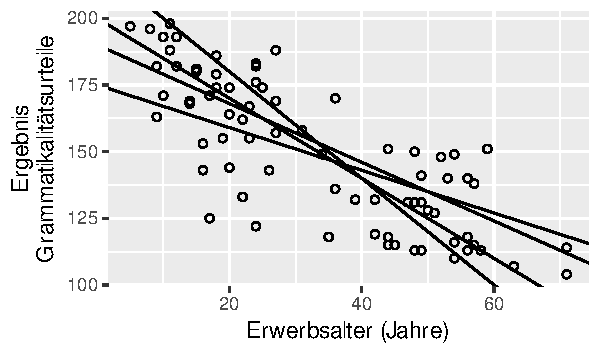
\includegraphics[width=.6\textwidth]{figs/unnamed-chunk-195-1} 

}

\caption{Wenn man von Hand eine gerade Linie durch die Punktwolke ziehen würde, zeichnet jeder die Linie wohl an einer anderen Stelle. Wir können aber Kriterien festlegen, die bewirken, dass alle die gleiche Linie zeichnen.\label{fig:differentregressions}}\label{fig:unnamed-chunk-195}
\end{figure}

\end{knitrout}

\subsection{Die einfache Regressionsgleichung}
Ähnlich wie im letzten Kapitel können wir eine Gleichung
aufschreiben, die die Datenpunkte in zwei Teile zerlegt:
einen systematischen Teil, der die Gemeinsamkeiten zwischen allen Werten ausdrückt,
und einen unsystematischen Teil, der die individuellen Unterschiede zwischen diesen
Gemeinsamkeiten und den Werten ausdrückt. Diesmal können
wir den Zusammenhang zwischen AOA und GJT als eine Gemeinsamkeit
im Datensatz betrachten. Dieser Zusammenhang scheint linear,
weshalb er als eine gerade Linie modelliert werden kann:
\[
\textrm{Wert} = \textrm{Gemeinsamkeit (inkl. AOA-Zusammenhang)} + \textrm{Abweichung}.
\]

Eine gerade Linie wird definiert durch
einen Schnittpunkt ($\beta_0$; dies ist der $y$-Wert, wenn $x = 0$)
und eine Steigung ($\beta_1$; diese sagt, um
wie viele Punkte $y$ steigt, wenn $x$ um eine Einheit erhöht wird);
siehe Abbildung \ref{fig:gerade}.

\begin{knitrout}
\definecolor{shadecolor}{rgb}{0.969, 0.969, 0.969}\color{fgcolor}\begin{figure}[tp]

{\centering 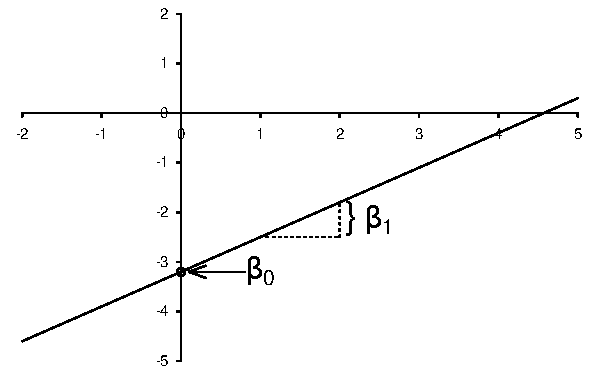
\includegraphics[width=.6\textwidth]{figs/unnamed-chunk-196-1} 

}

\caption{Schnittpunkt und Steigung einer Geraden.\label{fig:gerade}}\label{fig:unnamed-chunk-196}
\end{figure}

\end{knitrout}

Egal, wie wir $\beta_0$ und $\beta_1$ wählen: Die Linie $y_i = \beta_0 + \beta_1 x_i$ wird die
Daten nicht perfekt beschreiben: Es wird noch einen Restfehler ($\varepsilon$) geben.
Jeder $y$-Wert ($y_1$, $y_2$ etc.) kann also umschrieben werden
als die Kombination eines systematischen Teils ($\beta_0+\beta_1 x_i$)
und eines Restfehlers:
\begin{equation}\label{eq:simpleregression}
y_i = \beta_0 + \beta_1 x_i + \varepsilon_i.
\end{equation}
Diese mathematische Beschreibung ist ein einfaches lineares Modell:
`einfach', weil $y$ nur eine Funktion einer (statt mehrerer) Variablen ($x$) ist,
und `linear', weil $y$ als eine Summe (und nicht etwa ein
Produkt oder etwas Komplexeres) verschiedener Terme modelliert wird.

\subsection{Die Parameter schätzen}
$\beta_0$ und $\beta_1$ sind die \textbf{Parameter} der einfachen Regressionsgleichung,
und unsere nächste Aufgabe ist es, diese Parameter so gut wie möglich zu schätzen.
Dass wir diese Parameter nur schätzen und nicht wissen können, zeigt sich
in einem Gedankenexperiment: Wenn wir die gleiche Studie nochmals
unter den gleichen Bedingungen durchführen
würden, aber mit anderen Teilnehmenden, würde das Streudiagramm ja nicht identisch
aussehen. Wir würden aber davon ausgehen, dass beide Studien uns Informationen
über den `wahren' Zusammenhang zwischen AOA und GJT in dieser Population liefern.
Dieser `wahre' Zusammenhang---so unsere Annahme---wird durch die obige Regressionsgleichung
beschrieben, aber auf der Basis empirischer Forschung kann der
Zusammenhang höchstens approximiert werden.

Im Prinzip gibt es unendlich viele Möglichkeiten, $\beta_0$ und $\beta_1$ auszuwählen,
sodass die Gleichung aufgeht (wie Abbildung \ref{fig:differentregressions} illustriert),
aber uns interessieren nur die $\beta_0$- und $\beta_1$-Werte der optimalen Geraden.
Um diese zu schätzen, müssen wir definieren, was `optimal' in diesem Kontext heisst.
Wie im letzten Kapitel besprochen wurde, ist das am meisten verwendete Optimierungskriterion die Methode der kleinsten Quadrate, wonach die optimale Linie jene Gerade ist,
die die Summe der quadrierten Restfehler ($\sum_{i = 1}^{n} \widehat{\varepsilon_i}^2$) minimiert.
Wir können diese Summe für unterschiedliche Kombinationen
von $\widehat{\beta_0}$- und $\widehat{\beta_1}$-Werten berechnen.
\begin{itemize}
\item Sind  $\widehat{\beta_0} = 185$ und  $\widehat{\beta_1} = -2$,
dann ist
\[\sum_{i = 1}^{n} \widehat{\varepsilon_i}^2 = \sum_{i = 1}^{n} (y_i - (185 - 2x_i))^2 = 107121.
\]
In R berechnet man dies so:
\begin{knitrout}
\definecolor{shadecolor}{rgb}{0.969, 0.969, 0.969}\color{fgcolor}\begin{kframe}
\begin{alltt}
\hlstd{> }\hlkwd{sum}\hlstd{((d}\hlopt{$}\hlstd{GJT} \hlopt{-} \hlstd{(}\hlnum{185} \hlopt{-} \hlnum{2}\hlopt{*}\hlstd{d}\hlopt{$}\hlstd{AOA))}\hlopt{^}\hlnum{2}\hlstd{)}
\end{alltt}
\begin{verbatim}
[1] 107121
\end{verbatim}
\end{kframe}
\end{knitrout}

\item Sind  $\widehat{\beta_0} = 190$ und  $\widehat{\beta_1} = -1.5$,
dann ist
\[
\sum_{i = 1}^{n} \widehat{\varepsilon_i}^2 = \sum_{i = 1}^{n} (y_i - (190 - 1.5x_i))^2 = 28810.
\]
In R:
\begin{knitrout}
\definecolor{shadecolor}{rgb}{0.969, 0.969, 0.969}\color{fgcolor}\begin{kframe}
\begin{alltt}
\hlstd{> }\hlkwd{sum}\hlstd{((d}\hlopt{$}\hlstd{GJT} \hlopt{-} \hlstd{(}\hlnum{190} \hlopt{-} \hlnum{1.5}\hlopt{*}\hlstd{d}\hlopt{$}\hlstd{AOA))}\hlopt{^}\hlnum{2}\hlstd{)}
\end{alltt}
\begin{verbatim}
[1] 28810.25
\end{verbatim}
\end{kframe}
\end{knitrout}
\end{itemize}

$\widehat{\beta} = (190, -1.5)$ ist also optimaler
als $\widehat{\beta} = (180, -2)$.
Abbildung \ref{fig:ols} zeigt die Summe der quadrierten Restfehler
für unterschiedliche  $(\widehat{\beta_0}, \widehat{\beta_1})$-Kombinationen;
Kombinationen nahe bei $(190, -1.2)$ haben die kleinste Summe der quadrierten Restfehler.

\begin{knitrout}
\definecolor{shadecolor}{rgb}{0.969, 0.969, 0.969}\color{fgcolor}\begin{figure}[t]

{\centering 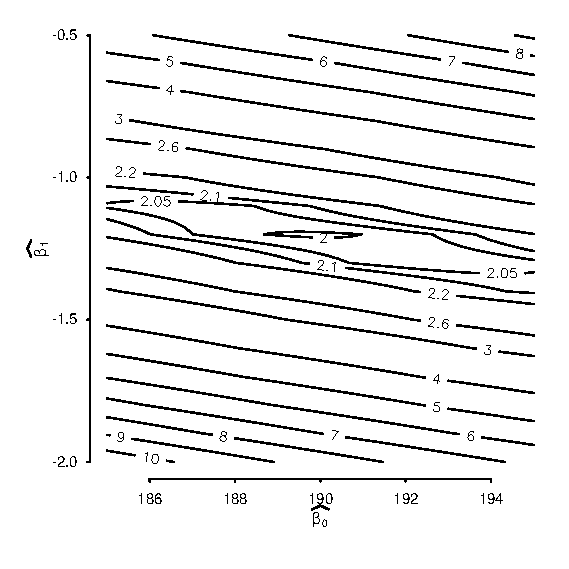
\includegraphics[width=.7\textwidth]{figs/unnamed-chunk-199-1} 

}

\caption{Die Summe der quadrierten Restfehler (geteilt durch 10'000) der GJT-Daten für unterschiedliche Parameterschätzungen. Diese Grafik kann wie eine topografische Karte gelesen werden; die Linien sind sozusagen Höhenlinien. Für Schnittpunkte nahe bei 190 und Steigungen nahe bei $-1.2$ wird diese Summe minimiert; bei diesen Koordinaten gibt es sozusagen einen Kessel.\label{fig:ols}}\label{fig:unnamed-chunk-199}
\end{figure}

\end{knitrout}

In der Praxis ackert man nicht zig Parameterkombinationen durch,
um die optimale zu finden. Der Vorteil der Methode der kleinsten
Quadrate ist, dass man die optimalen Parameterschätzungen schnell
analytisch finden kann, und zwar so:
\begin{equation*}
 \widehat{\beta_1} = r_{xy}\frac{s_y}{s_x},
\end{equation*}
\begin{equation}\label{eq:intercept}
 \widehat{\beta_0} = \bar{y} - \widehat{\beta_1} \bar{x}.
\end{equation}

Hier steht $r_{xy}$ für die Pearsonkorrelation zwischen $x$ und $y$
in der Stichprobe. $s_x, s_y$ stehen für die Stichprobenstandardabweichungen
von $x$ bzw.\ $y$. $\bar{x}$ ist das Stichprobenmittel von $x$.
Der
\href{http://en.wikipedia.org/wiki/Simple_linear_regression#Fitting_the_regression_line}{Beweis}
für diese Formeln wird hier nicht reproduziert.
Für die Daten von \citet{DeKeyser2010} sieht das Ergebnis
dieser Berechnungen so aus:
\begin{knitrout}
\definecolor{shadecolor}{rgb}{0.969, 0.969, 0.969}\color{fgcolor}\begin{kframe}
\begin{alltt}
\hlstd{> }\hlstd{beta1_hat} \hlkwb{<-} \hlkwd{cor}\hlstd{(d}\hlopt{$}\hlstd{AOA, d}\hlopt{$}\hlstd{GJT)} \hlopt{*} \hlkwd{sd}\hlstd{(d}\hlopt{$}\hlstd{GJT)} \hlopt{/} \hlkwd{sd}\hlstd{(d}\hlopt{$}\hlstd{AOA)}
\hlstd{> }\hlstd{beta1_hat}
\end{alltt}
\begin{verbatim}
[1] -1.217977
\end{verbatim}
\begin{alltt}
\hlstd{> }\hlstd{beta0_hat} \hlkwb{<-} \hlkwd{mean}\hlstd{(d}\hlopt{$}\hlstd{GJT)} \hlopt{-} \hlstd{beta1_hat} \hlopt{*} \hlkwd{mean}\hlstd{(d}\hlopt{$}\hlstd{AOA)}
\hlstd{> }\hlstd{beta0_hat}
\end{alltt}
\begin{verbatim}
[1] 190.4086
\end{verbatim}
\end{kframe}
\end{knitrout}

Einfacher geht es mit der \texttt{lm()}-Funktion:
\begin{knitrout}
\definecolor{shadecolor}{rgb}{0.969, 0.969, 0.969}\color{fgcolor}\begin{kframe}
\begin{alltt}
\hlstd{> }\hlstd{aoa.lm} \hlkwb{<-} \hlkwd{lm}\hlstd{(GJT} \hlopt{~} \hlstd{AOA,} \hlkwc{data} \hlstd{= d)}
\hlstd{> }\hlstd{aoa.lm}
\end{alltt}
\begin{verbatim}

Call:
lm(formula = GJT ~ AOA, data = d)

Coefficients:
(Intercept)          AOA  
    190.409       -1.218  
\end{verbatim}
\end{kframe}
\end{knitrout}

\texttt{(Intercept)} ist hier $\widehat{\beta_0}$, also
der Schnittpunkt der Regressionsgeraden mit der $y$-Achse.
\texttt{AOA} ist $\widehat{\beta_1}$ und zeigt, um wie viele
Einheiten die Gerade steigt oder senkt, wenn man entlang
der \texttt{AOA}-Achse eine Einheit nach rechts geht.

\section{Regressionsgeraden zeichnen}
Das Ergebnis einer Regressionsanalyse kann auch grafisch dargestellt
werden, indem man dem Streudiagramm die Regressionsgerade hinzufügt
(Abbildung \ref{fig:scatterwithreg}):
\begin{knitrout}
\definecolor{shadecolor}{rgb}{0.969, 0.969, 0.969}\color{fgcolor}\begin{kframe}
\begin{alltt}
\hlstd{> }\hlkwd{ggplot}\hlstd{(}\hlkwc{data} \hlstd{= d,}
\hlstd{+ }       \hlkwd{aes}\hlstd{(}\hlkwc{x} \hlstd{= AOA,}
\hlstd{+ }           \hlkwc{y} \hlstd{= GJT))} \hlopt{+}
\hlstd{+ }  \hlkwd{geom_point}\hlstd{(}\hlkwc{shape} \hlstd{=} \hlnum{1}\hlstd{)} \hlopt{+}
\hlstd{+ }  \hlcom{# Mit geom_abline() wird dem Streudiagramm eine Gerade hinzugefügt.}
\hlstd{+ }  \hlkwd{geom_abline}\hlstd{(}\hlkwc{intercept} \hlstd{=} \hlnum{190.41}\hlstd{,} \hlkwc{slope} \hlstd{=} \hlopt{-}\hlnum{1.218}\hlstd{)}
\end{alltt}
\end{kframe}\begin{figure}[tp]

{\centering 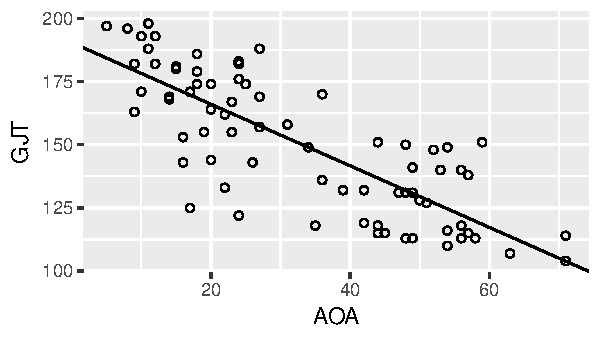
\includegraphics[width=.6\textwidth]{figs/unnamed-chunk-202-1} 

}

\caption{Ein Streudiagramm mit einer Regressionsgeraden. Die Regressionsgerade erfasst die modellierte zentrale Tendenz (genauer: das GJT-Mittel) für die unterschiedlichen AOA-Werte.\label{fig:scatterwithreg}}\label{fig:unnamed-chunk-202}
\end{figure}

\end{knitrout}

Eine alternative Methode ist die folgende.
Wenn man bei \texttt{geom\_smooth()} als Methode \texttt{"lm"} einstellt,
wird das Regressionsmodell von \texttt{ggplot()} berechnet.
Im Code unten habe ich den Parameter \texttt{se} auf \texttt{FALSE}
gestellt; im nächsten Abschnitt wird klar warum.
\begin{knitrout}
\definecolor{shadecolor}{rgb}{0.969, 0.969, 0.969}\color{fgcolor}\begin{kframe}
\begin{alltt}
\hlstd{> }\hlcom{# Nicht gezeichnet}
\hlstd{> }\hlkwd{ggplot}\hlstd{(}\hlkwc{data} \hlstd{= d,}
\hlstd{+ }       \hlkwd{aes}\hlstd{(}\hlkwc{x} \hlstd{= AOA,} \hlkwc{y} \hlstd{= GJT))} \hlopt{+}
\hlstd{+ }  \hlkwd{geom_point}\hlstd{(}\hlkwc{shape} \hlstd{=} \hlnum{1}\hlstd{)} \hlopt{+}
\hlstd{+ }  \hlkwd{geom_smooth}\hlstd{(}\hlkwc{method} \hlstd{=} \hlstr{"lm"}\hlstd{,} \hlkwc{se} \hlstd{=} \hlnum{FALSE}\hlstd{)}
\end{alltt}
\end{kframe}
\end{knitrout}

Aber was stellt diese Gerade genau dar?  Mit dem Regressionsmodell versuchten
wir die GJT-Werte ($y_i$) als eine Funktion der AOA-Werte ($x_i$) und eines
Restfehlers ($\varepsilon_i$) zu modellieren:
\[
y_i = \widehat{\beta_0} + \widehat{\beta_1}x_i + \widehat{\varepsilon_i}.
\]

Auf der Regressionsgeraden ($\widehat{\beta_0} + \widehat{\beta_1}x_i$)
liegen die $y_i$-Werte abzüglich des Restfehlers, also
\[
\widehat{y_i} = \widehat{\beta_0} + \widehat{\beta_1}x_i.
\]
Wie man diese $\widehat{y_i}$-Werte konzeptuell interpretieren
kann, ist einfacher zu erklären, wenn wir uns zuerst anschauen, wie
man die Unsicherheit in den Parameterschätzungen quantifizieren kann.

\subsection{Unsicherheit in Parameterschätzungen schätzen}
Die Parameterschätzungen $\widehat{\beta}$ werden aufgrund
des Stichprobenfehlers von Stichprobe zu Stichprobe mehr oder
weniger voneinander abweichen. Da $\widehat{\beta}$ aus Schätzungen
besteht, ist auch die Regressionsgerade nur eine Schätzung.
Um die Unsicherheit in den Parameterschätzungen und in der Regressionsgeraden
zu quantifizieren, können wir uns wiederum auf den Bootstrap oder
auf algebraische Methoden verlassen.

\subsubsection{Mit dem Bootstrap}
Das Bootstrappen eines linearen Modells mit einem Prädiktor
verläuft analog zum Bootstrappen eines linearen Modells ohne Prädiktor.
Zuerst wird hier die Methode aus Abschnitt \ref{bootstrapoverview}
(semi-parametrischer Bootstrap)
aufs lineare Modell mit einem Prädiktor angewandt:
\begin{enumerate}\label{nonparametricbsregression}
 \item Man berechnet $\widehat{\beta}$ (also $\widehat{\beta_0}$ und $\widehat{\beta_1}$) und erhält dazu auch noch $\widehat{\varepsilon}$.
 \item Man zieht eine Bootstrap-Stichprobe aus $\widehat{\varepsilon}$.
 Nenne diese $\widehat{\varepsilon}^{*}$.
 \item Man kombiniert $\widehat{\beta_0}$, $\widehat{\beta_1}x_i$  und $\widehat{\varepsilon}^{*}$. Dies ergibt
 eine neue Reihe von $y$-Werten: $y_i^{*} = \widehat{\beta_0} + \widehat{\beta_1}x_i + \widehat{\varepsilon_i}^{*}$.
 \item Auf der Basis von $y_i^{*}$ wird $\widehat{\beta}$ erneut geschätzt.
 \item Schritte 2--4 werden ein paar tausend Mal ausgeführt, sodass man die Verteilung der gebootstrappten $\beta$-Schätzungen erhält.
\end{enumerate}

In R-Code:
\begin{knitrout}
\definecolor{shadecolor}{rgb}{0.969, 0.969, 0.969}\color{fgcolor}\begin{kframe}
\begin{alltt}
\hlstd{> }\hlstd{runs} \hlkwb{<-} \hlnum{20000}
\hlstd{> }
\hlstd{> }\hlcom{# Wir werden 20'000 Bootstrapschätzungen pro Parameter haben.}
\hlstd{> }\hlcom{# Diese speichern wir in einer Matrix mit 20'000 Zeilen und 2 Spalten.}
\hlstd{> }\hlstd{bs_beta} \hlkwb{<-} \hlkwd{matrix}\hlstd{(}\hlkwc{nrow} \hlstd{= runs,} \hlkwc{ncol} \hlstd{=} \hlnum{2}\hlstd{)}
\hlstd{> }
\hlstd{> }\hlkwa{for} \hlstd{(i} \hlkwa{in} \hlnum{1}\hlopt{:}\hlstd{runs) \{}
\hlstd{+ }  \hlcom{# Residuen des Modells bootstrappen (resampling with replacement)}
\hlstd{+ }  \hlstd{bs_residuals} \hlkwb{<-} \hlkwd{sample}\hlstd{(}\hlkwd{resid}\hlstd{(aoa.lm),}
\hlstd{+ }                         \hlkwc{size} \hlstd{=} \hlkwd{length}\hlstd{(}\hlkwd{resid}\hlstd{(aoa.lm)),}
\hlstd{+ }                         \hlkwc{replace} \hlstd{=} \hlnum{TRUE}\hlstd{)}

\hlstd{+ }  \hlcom{# Modellvorhersagen mit gebootstrappten Residuen kombinieren}
\hlstd{+ }  \hlstd{bs_GJT} \hlkwb{<-} \hlkwd{predict}\hlstd{(aoa.lm)} \hlopt{+} \hlstd{bs_residuals}

\hlstd{+ }  \hlcom{# Modell neu rechnen mit gebootstrappten GJT-Daten.}
\hlstd{+ }  \hlcom{# d$AOA enthält die AOA-Daten des ursprünglichen Datensatzes}
\hlstd{+ }  \hlcom{# und zählt also 76 Beobachtungen.}
\hlstd{+ }  \hlstd{resampled.lm} \hlkwb{<-} \hlkwd{lm}\hlstd{(bs_GJT} \hlopt{~} \hlstd{d}\hlopt{$}\hlstd{AOA)}

\hlstd{+ }  \hlcom{# Parameterschätzungen in neue Zeile der Matrix speichern:}
\hlstd{+ }  \hlstd{bs_beta[i, ]} \hlkwb{<-} \hlkwd{coef}\hlstd{(resampled.lm)}
\hlstd{+ }\hlstd{\}}
\hlstd{> }\hlcom{# Erste 6 Zeilen anzeigen:}
\hlstd{> }\hlkwd{head}\hlstd{(bs_beta)}
\end{alltt}
\begin{verbatim}
         [,1]      [,2]
[1,] 191.8229 -1.289491
[2,] 184.2666 -1.053764
[3,] 187.7258 -1.161843
[4,] 185.9599 -1.181903
[5,] 197.2874 -1.446598
[6,] 182.4883 -1.085926
\end{verbatim}
\end{kframe}
\end{knitrout}
Man bemerke übrigens die Verwendung von `[' statt
`[[' in der letzten Zeile der \textit{for}-Schleife: Jetzt schreiben
wir nämlich mehr als einen Wert in die Matrix.

Die Verteilungen der Bootstrapschätzungen können wie gehabt
mit Histogrammen gezeichnet werden; siehe Abbildung \ref{fig:bootstrapdistributiondekeyser}.\label{sec:histogrammebootstrapdekeyser}

\begin{knitrout}
\definecolor{shadecolor}{rgb}{0.969, 0.969, 0.969}\color{fgcolor}\begin{kframe}
\begin{alltt}
\hlstd{> }\hlcom{# Ergebnisse in tibble giessen}
\hlstd{> }\hlstd{bs_beta_tbl} \hlkwb{<-} \hlkwd{tibble}\hlstd{(}\hlkwc{Schnittpunkt} \hlstd{= bs_beta[,} \hlnum{1}\hlstd{],}
\hlstd{+ }                      \hlkwc{Steigung} \hlstd{= bs_beta[,} \hlnum{2}\hlstd{])}
\hlstd{> }
\hlstd{> }\hlcom{# Grafik zeichnen}
\hlstd{> }\hlstd{bs_beta_tbl |>}
\hlstd{+ }  \hlcom{# Schätzungen alle in gleiche Spalte}
\hlstd{+ }  \hlkwd{pivot_longer}\hlstd{(}\hlkwc{cols} \hlstd{=} \hlkwd{everything}\hlstd{(),}
\hlstd{+ }               \hlkwc{names_to} \hlstd{=} \hlstr{"Parameter"}\hlstd{,}
\hlstd{+ }               \hlkwc{values_to} \hlstd{=} \hlstr{"Estimate"}\hlstd{) |>}
\hlstd{+ }  \hlkwd{ggplot}\hlstd{(}\hlkwd{aes}\hlstd{(}\hlkwc{x} \hlstd{= Estimate))} \hlopt{+}
\hlstd{+ }  \hlkwd{geom_histogram}\hlstd{(}\hlkwc{fill} \hlstd{=} \hlstr{"lightgrey"}\hlstd{,} \hlkwc{col} \hlstd{=} \hlstr{"black"}\hlstd{,} \hlkwc{bins} \hlstd{=} \hlnum{50}\hlstd{)} \hlopt{+}
\hlstd{+ }  \hlcom{# facet_wrap zeichnet separate Grafiken je nach (hier) Parameter}
\hlstd{+ }  \hlkwd{facet_wrap}\hlstd{(}\hlkwd{vars}\hlstd{(Parameter),} \hlkwc{scales} \hlstd{=} \hlstr{"free"}\hlstd{)} \hlopt{+}
\hlstd{+ }  \hlkwd{xlab}\hlstd{(}\hlstr{"Bootstrapschätzung"}\hlstd{)} \hlopt{+}
\hlstd{+ }  \hlkwd{ylab}\hlstd{(}\hlstr{"Anzahl"}\hlstd{)}
\end{alltt}
\end{kframe}\begin{figure}[tp]

{\centering 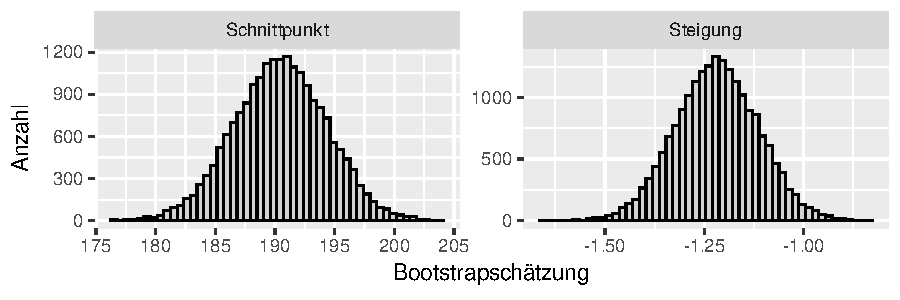
\includegraphics[width=.7\textwidth]{figs/unnamed-chunk-205-1} 

}

\caption{Verteilung der Bootstrap-Schätzungen der Parameter im Regressionsmodell \texttt{aoa.lm}.\label{fig:bootstrapdistributiondekeyser}}\label{fig:unnamed-chunk-205}
\end{figure}

\end{knitrout}

Da diese Verteilungen normalverteilt aussehen,
können die Konfidenzintervalle (hier: 90\%)
sowohl mit der \texttt{quantile()}- als
auch mit der \texttt{qnorm()}-Funktion berechnet werden;
die Ergebnisse sind einander nahezu identisch.
\begin{knitrout}
\definecolor{shadecolor}{rgb}{0.969, 0.969, 0.969}\color{fgcolor}\begin{kframe}
\begin{alltt}
\hlstd{> }\hlcom{# Perzentilmethode}
\hlstd{> }\hlkwd{quantile}\hlstd{(bs_beta_tbl}\hlopt{$}\hlstd{Schnittpunkt,} \hlkwc{probs} \hlstd{=} \hlkwd{c}\hlstd{(}\hlnum{0.05}\hlstd{,} \hlnum{0.95}\hlstd{))} \hlcom{# Schnittpunkt}
\end{alltt}
\begin{verbatim}
      5%      95% 
184.0892 196.7159 
\end{verbatim}
\begin{alltt}
\hlstd{> }\hlkwd{quantile}\hlstd{(bs_beta_tbl}\hlopt{$}\hlstd{Steigung,} \hlkwc{probs} \hlstd{=} \hlkwd{c}\hlstd{(}\hlnum{0.05}\hlstd{,} \hlnum{0.95}\hlstd{))} \hlcom{# Steigung}
\end{alltt}
\begin{verbatim}
       5%       95% 
-1.388537 -1.049464 
\end{verbatim}
\begin{alltt}
\hlstd{> }\hlcom{# Kürzer mit apply(). Die '2' heisst, dass die Funktion}
\hlstd{> }\hlcom{# 'quantile' pro Spalte und nicht pro Zeile ausgeführt werden soll.}
\hlstd{> }\hlkwd{apply}\hlstd{(bs_beta,} \hlnum{2}\hlstd{, quantile,} \hlkwc{probs} \hlstd{=} \hlkwd{c}\hlstd{(}\hlnum{0.05}\hlstd{,} \hlnum{0.95}\hlstd{))}
\end{alltt}
\begin{verbatim}
        [,1]      [,2]
5%  184.0892 -1.388537
95% 196.7159 -1.049464
\end{verbatim}
\end{kframe}
\end{knitrout}

\texttt{coef(aoa.lm)} gibt zwei Werte aus:
die Schätzung des Schnittpunkts und die Schätzung der Steigung:
\begin{knitrout}
\definecolor{shadecolor}{rgb}{0.969, 0.969, 0.969}\color{fgcolor}\begin{kframe}
\begin{alltt}
\hlstd{> }\hlkwd{coef}\hlstd{(aoa.lm)}
\end{alltt}
\begin{verbatim}
(Intercept)         AOA 
 190.408634   -1.217977 
\end{verbatim}
\end{kframe}
\end{knitrout}

Um den ersten Wert zu selektieren, kann auch \texttt{coef(aoa.lm)[[1]]}
verwendet werden, daher:
\begin{knitrout}
\definecolor{shadecolor}{rgb}{0.969, 0.969, 0.969}\color{fgcolor}\begin{kframe}
\begin{alltt}
\hlstd{> }\hlcom{# qnorm}
\hlstd{> }\hlkwd{coef}\hlstd{(aoa.lm)[[}\hlnum{1}\hlstd{]]} \hlopt{+} \hlkwd{qnorm}\hlstd{(}\hlkwd{c}\hlstd{(}\hlnum{0.05}\hlstd{,} \hlnum{0.95}\hlstd{))} \hlopt{*} \hlkwd{sd}\hlstd{(bs_beta_tbl}\hlopt{$}\hlstd{Schnittpunkt)}
\end{alltt}
\begin{verbatim}
[1] 184.0646 196.7527
\end{verbatim}
\begin{alltt}
\hlstd{> }\hlkwd{coef}\hlstd{(aoa.lm)[[}\hlnum{2}\hlstd{]]} \hlopt{+} \hlkwd{qnorm}\hlstd{(}\hlkwd{c}\hlstd{(}\hlnum{0.05}\hlstd{,} \hlnum{0.95}\hlstd{))} \hlopt{*} \hlkwd{sd}\hlstd{(bs_beta_tbl}\hlopt{$}\hlstd{Steigung)}
\end{alltt}
\begin{verbatim}
[1] -1.388678 -1.047275
\end{verbatim}
\end{kframe}
\end{knitrout}

Die Standardabweichungen der Bootstrapschätzungen schätzen den relevanten
Standardfehler:
\begin{knitrout}
\definecolor{shadecolor}{rgb}{0.969, 0.969, 0.969}\color{fgcolor}\begin{kframe}
\begin{alltt}
\hlstd{> }\hlkwd{apply}\hlstd{(bs_beta,} \hlnum{2}\hlstd{, sd)}
\end{alltt}
\begin{verbatim}
[1] 3.856910 0.103779
\end{verbatim}
\end{kframe}
\end{knitrout}

Die Bootstrapschätzungen können auch verwendet werden,
um die Unsicherheit in der Regressionsgeraden grafisch darzustellen.
Wir können zum Beispiel die Bootstrapschätzung des Schnittpunktes
und der Steigung abrufen und anhand derer Regressionsgeraden zeichnen.
Der Übersichtlichkeit halber werden hier nur die ersten vier Bootstrapschätzungen
gezeigt. Bei Ihnen werden diese aufgrund der Zufälligkeit im
Bootstrap natürlich anders aussehen.
Die entsprechenden Regressionsgeraden sieht man in Abbildung
\ref{fig:bootstrapregressionline}:
\begin{knitrout}
\definecolor{shadecolor}{rgb}{0.969, 0.969, 0.969}\color{fgcolor}\begin{kframe}
\begin{alltt}
\hlstd{> }\hlkwd{head}\hlstd{(bs_beta,} \hlnum{4}\hlstd{)}
\end{alltt}
\begin{verbatim}
         [,1]      [,2]
[1,] 191.8229 -1.289491
[2,] 184.2666 -1.053764
[3,] 187.7258 -1.161843
[4,] 185.9599 -1.181903
\end{verbatim}
\end{kframe}
\end{knitrout}

\begin{knitrout}
\definecolor{shadecolor}{rgb}{0.969, 0.969, 0.969}\color{fgcolor}\begin{figure}[tp]

{\centering 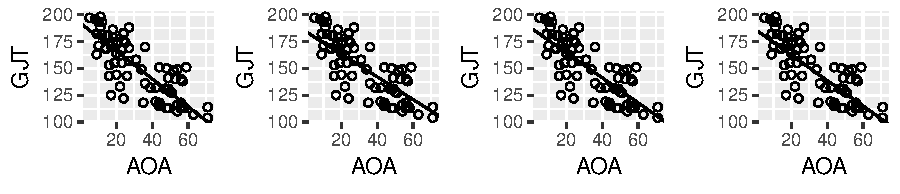
\includegraphics[width=\textwidth]{figs/unnamed-chunk-211-1} 

}

\caption{Regressionsgeraden, die anhand der 1., 2., 3.\ und 4.\ Bootstrapschätzungen des Schnittpunktes und der Steigung gezeichnet wurden. Die Grafiken sind einander recht ähnlich, aber nicht identisch.\label{fig:bootstrapregressionline}}\label{fig:unnamed-chunk-211}
\end{figure}

\end{knitrout}

In Abbildung \ref{fig:bootstrapregressionline100} mache ich nochmals
das Gleiche, aber diesmal mit 100 Schätzungen.
Für die Interessierten zeige ich diesmal auch den Code. Wie Sie sehen können,
kommen die Regressionsgeraden
für durchschnittliche AOA-Werte
einander ziemlich nahe, aber nahe
den Minimum- und Maximumwerten fächern sie sich auf.

\begin{knitrout}
\definecolor{shadecolor}{rgb}{0.969, 0.969, 0.969}\color{fgcolor}\begin{kframe}
\begin{alltt}
\hlstd{> }\hlstd{plot_konfidenzband} \hlkwb{<-} \hlkwd{ggplot}\hlstd{(}\hlkwc{data} \hlstd{= d,}
\hlstd{+ }                             \hlkwd{aes}\hlstd{(}\hlkwc{x} \hlstd{= AOA,} \hlkwc{y} \hlstd{= GJT))} \hlopt{+}
\hlstd{+ }  \hlkwd{geom_point}\hlstd{(}\hlkwc{shape} \hlstd{=} \hlnum{1}\hlstd{)}
\hlstd{> }
\hlstd{> }\hlkwa{for} \hlstd{(i} \hlkwa{in} \hlnum{1}\hlopt{:}\hlnum{100}\hlstd{) \{}
\hlstd{+ }  \hlstd{plot_konfidenzband} \hlkwb{<-} \hlstd{plot_konfidenzband} \hlopt{+}
\hlstd{+ }    \hlkwd{geom_abline}\hlstd{(}\hlkwc{intercept} \hlstd{= bs_beta[i,} \hlnum{1}\hlstd{],}
\hlstd{+ }                \hlkwc{slope} \hlstd{= bs_beta[i,} \hlnum{2}\hlstd{],}
\hlstd{+ }                \hlkwc{alpha} \hlstd{=} \hlnum{1}\hlopt{/}\hlnum{30}\hlstd{)}
\hlstd{+ }\hlstd{\}}
\hlstd{> }\hlstd{plot_konfidenzband}
\end{alltt}
\end{kframe}\begin{figure}[tp]

{\centering 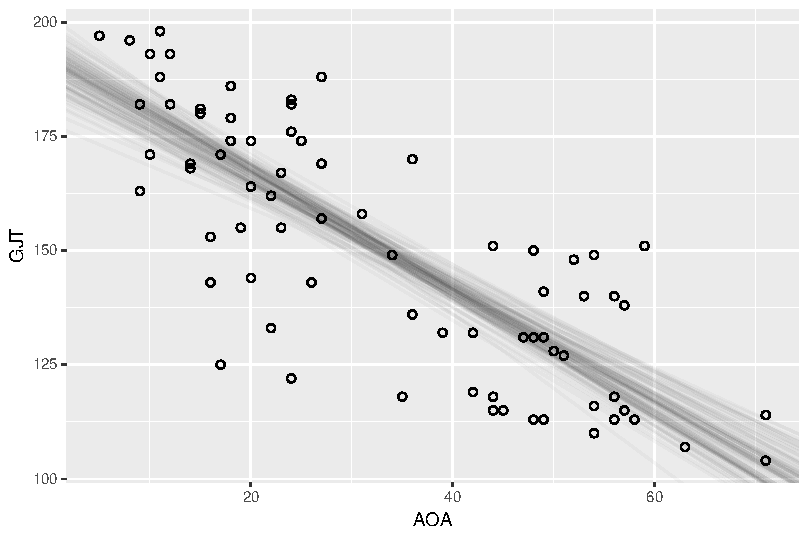
\includegraphics[width=.7\textwidth]{figs/unnamed-chunk-212-1} 

}

\caption{Regressionsgeraden, die auf der Basis von 100 Bootstrapschätzungen des Schnittpunktes und der Steigung gezeichnet wurden.\label{fig:bootstrapregressionline100}}\label{fig:unnamed-chunk-212}
\end{figure}

\end{knitrout}
Statt diese Regressionsgeraden einzeln darzustellen,
färbt man in der Regel das Band, in das diese Geraden mehrheitlich fallen,
ein. Analog zum Konfidenzintervall nennt man dieses dann ein
\textbf{Konfidenzband}. Der nächste Abschnitt erklärt, wie man
Konfidenzbänder mittels Bootstrapping konstruieren kann, aber dieses
können Sie gerne überspringen.

\paragraph{Konfidenzbänder mit dem Bootstrap konstruieren.}
Die Idee ist die folgende.
Man definiert eine Reihe von $x$-Werten, an denen man
das Konfidenzband zeichnen möchte. In unserem Fall handelt
es sich einfach um eine Handvoll Zahlen zwischen dem AOA-Minimum
und dem AOA-Maximum. Es spielt hier keine grosse Rolle, wie
viele Werte man festlegt.
\begin{knitrout}
\definecolor{shadecolor}{rgb}{0.969, 0.969, 0.969}\color{fgcolor}\begin{kframe}
\begin{alltt}
\hlstd{> }\hlstd{neue_aoa} \hlkwb{<-} \hlkwd{seq}\hlstd{(}\hlkwc{from} \hlstd{=} \hlkwd{min}\hlstd{(d}\hlopt{$}\hlstd{AOA),} \hlkwc{to} \hlstd{=} \hlkwd{max}\hlstd{(d}\hlopt{$}\hlstd{AOA),} \hlkwc{by} \hlstd{=} \hlnum{1}\hlstd{)}
\hlstd{> }\hlcom{# also 5, 6, 7, etc., 69, 70, 71}
\end{alltt}
\end{kframe}
\end{knitrout}

Man nimmt die Bootstrapschätzungen des Schnittpunkts
($\widehat{\beta_0}^{*}$) und der Steigung ($\widehat{\beta_1}^{*}$)
und man berechnet für jedes Paar von Schätzungen
den $\widehat{y}$-Wert für jeden $x$-Wert. Zum Beispiel
ist (in meinem Fall) das erste Paar Bootstrapschätzungen:
\begin{knitrout}
\definecolor{shadecolor}{rgb}{0.969, 0.969, 0.969}\color{fgcolor}\begin{kframe}
\begin{alltt}
\hlstd{> }\hlstd{bs_beta[}\hlnum{1}\hlstd{, ]}
\end{alltt}
\begin{verbatim}
[1] 191.822911  -1.289491
\end{verbatim}
\end{kframe}
\end{knitrout}

Der Vektor von $\widehat{y}$-Werten für dieses Paar
von Bootstrapschätzungen ist daher:
\begin{knitrout}
\definecolor{shadecolor}{rgb}{0.969, 0.969, 0.969}\color{fgcolor}\begin{kframe}
\begin{alltt}
\hlstd{> }\hlcom{# 191.82 + (-1.29) * 5, 191.82 + (-1.29) * 6, usw.}
\hlstd{> }\hlstd{bs_beta[}\hlnum{1}\hlstd{,} \hlnum{1}\hlstd{]} \hlopt{+} \hlstd{bs_beta[}\hlnum{1}\hlstd{,} \hlnum{2}\hlstd{]} \hlopt{*} \hlstd{neue_aoa}
\end{alltt}
\begin{verbatim}
 [1] 185.3755 184.0860 182.7965 181.5070 180.2175 178.9280
 [7] 177.6385 176.3490 175.0595 173.7700 172.4805 171.1910
[13] 169.9016 168.6121 167.3226 166.0331 164.7436 163.4541
[19] 162.1646 160.8751 159.5856 158.2961 157.0066 155.7172
[25] 154.4277 153.1382 151.8487 150.5592 149.2697 147.9802
[31] 146.6907 145.4012 144.1117 142.8222 141.5327 140.2433
[37] 138.9538 137.6643 136.3748 135.0853 133.7958 132.5063
[43] 131.2168 129.9273 128.6378 127.3483 126.0589 124.7694
[49] 123.4799 122.1904 120.9009 119.6114 118.3219 117.0324
[55] 115.7429 114.4534 113.1639 111.8744 110.5850 109.2955
[61] 108.0060 106.7165 105.4270 104.1375 102.8480 101.5585
[67] 100.2690
\end{verbatim}
\end{kframe}
\end{knitrout}

Diese Übung machen wir für alle Paare von
Bootstrapschätzungen---in unserem Fall also 20'000 Mal.
Mit einer \textit{for}-Schleife kann man dies übersichtlich tun.
Da das Ergebnis jeder Iteration aber einen Vektor
mit so vielen Elementen wie (hier) \texttt{neue\_aoa} ist,
ist es praktischer, diese Werte in einer Matrix zu speichern
als in 20'000 Vektoren. Diese Schritte kann man auch mit
Matrizenalgebra ausführen, aber ich vermute, dass ein
\textit{for}-Schleife das Verfahren transparenter macht.
\begin{knitrout}
\definecolor{shadecolor}{rgb}{0.969, 0.969, 0.969}\color{fgcolor}\begin{kframe}
\begin{alltt}
\hlstd{> }\hlcom{# Matrix mit den Vorhersagen:}
\hlstd{> }\hlcom{# wir brauchen 20'000 Zeilen (Anzahl Bootstraps)}
\hlstd{> }\hlcom{# und so viele Spalten wie es vorherzusagende Werte pro Bootstrap gibt}
\hlstd{> }\hlstd{bs_y_hat} \hlkwb{<-} \hlkwd{matrix}\hlstd{(}\hlkwc{nrow} \hlstd{= runs,} \hlcom{# die Anzahl Bootstraps}
\hlstd{+ }                   \hlkwc{ncol} \hlstd{=} \hlkwd{length}\hlstd{(neue_aoa))} \hlcom{# die Anzahl y-hat-Werte}
\hlstd{> }
\hlstd{> }\hlcom{# Für jedes Paar von Bootstrapschätzungen,}
\hlstd{> }\hlkwa{for} \hlstd{(i} \hlkwa{in} \hlnum{1}\hlopt{:}\hlstd{runs) \{}
\hlstd{+ }  \hlcom{# berechne die 'vorhergesagten' y-Werte für}
\hlstd{+ }  \hlcom{# jedes Element von neue_aoa und speichere diese}
\hlstd{+ }  \hlstd{bs_y_hat[i, ]} \hlkwb{<-} \hlstd{bs_beta[i,} \hlnum{1}\hlstd{]} \hlopt{+} \hlstd{bs_beta[i,} \hlnum{2}\hlstd{]}\hlopt{*}\hlstd{neue_aoa}
\hlstd{+ }\hlstd{\}}
\end{alltt}
\end{kframe}
\end{knitrout}

Sie können diese Matrix mit etwa \texttt{head(bs\_y\_hat)} inspizieren.
Um das 95\%-Kon\-fi\-denz\-band zu konstruieren, schlagen wir nun das 2.5.\ und
das 97.5.\ Perzentil jeder Spalte nach.
Die 2.5.\ Perzentile bilden
die untere Grenze des Konfidenzbandes; die 97.5.\ die obere.
Dazu verwende ich hier die \texttt{apply()}-Funktion, mit der
man eine Funktion (hier \texttt{quantile()} mit dem Zusatzparameter \texttt{probs = 0.025})
bequem auf alle Spalten oder Zeilen einer Matrix (hier \texttt{bs\_y\_hat}) evaluieren kann.
Die Zahl \texttt{2} spezifiziert, dass die Funktion pro Spalte evaluiert werden soll;
\texttt{1} hiesse, dass sie pro Zeile zu evaluieren ist.
\begin{knitrout}
\definecolor{shadecolor}{rgb}{0.969, 0.969, 0.969}\color{fgcolor}\begin{kframe}
\begin{alltt}
\hlstd{> }\hlstd{unten_95} \hlkwb{<-} \hlkwd{apply}\hlstd{(bs_y_hat,} \hlnum{2}\hlstd{, quantile,} \hlkwc{probs} \hlstd{=} \hlnum{0.025}\hlstd{)}
\hlstd{> }\hlstd{oben_95} \hlkwb{<-} \hlkwd{apply}\hlstd{(bs_y_hat,} \hlnum{2}\hlstd{, quantile,} \hlkwc{probs} \hlstd{=} \hlnum{0.975}\hlstd{)}
\end{alltt}
\end{kframe}
\end{knitrout}

Das 80\%-Konfidenzband würde man so konstruieren:
\begin{knitrout}
\definecolor{shadecolor}{rgb}{0.969, 0.969, 0.969}\color{fgcolor}\begin{kframe}
\begin{alltt}
\hlstd{> }\hlstd{unten_80} \hlkwb{<-} \hlkwd{apply}\hlstd{(bs_y_hat,} \hlnum{2}\hlstd{, quantile,} \hlkwc{probs} \hlstd{=} \hlnum{0.10}\hlstd{)}
\hlstd{> }\hlstd{oben_80} \hlkwb{<-} \hlkwd{apply}\hlstd{(bs_y_hat,} \hlnum{2}\hlstd{, quantile,} \hlkwc{probs} \hlstd{=} \hlnum{0.90}\hlstd{)}
\end{alltt}
\end{kframe}
\end{knitrout}

Man kann auch noch das Mittel jeder Spalte berechnen. Dies
ergibt ungefähr die Regressionsgerade:
\begin{knitrout}
\definecolor{shadecolor}{rgb}{0.969, 0.969, 0.969}\color{fgcolor}\begin{kframe}
\begin{alltt}
\hlstd{> }\hlstd{mittel} \hlkwb{<-} \hlkwd{apply}\hlstd{(bs_y_hat,} \hlnum{2}\hlstd{, mean)}
\end{alltt}
\end{kframe}
\end{knitrout}

Wenn man die Grafik mit \texttt{ggplot2()} zeichnen möchte,
muss man diese Werte noch in ein tibble giessen:
\begin{knitrout}
\definecolor{shadecolor}{rgb}{0.969, 0.969, 0.969}\color{fgcolor}\begin{kframe}
\begin{alltt}
\hlstd{> }\hlstd{konfidenzband_tbl} \hlkwb{<-} \hlkwd{tibble}\hlstd{(neue_aoa, mittel,}
\hlstd{+ }                            \hlstd{unten_95, oben_95,}
\hlstd{+ }                            \hlstd{unten_80, oben_80)}
\end{alltt}
\end{kframe}
\end{knitrout}

Zeichnen kann man das Konfidenzband dann so:
\begin{knitrout}
\definecolor{shadecolor}{rgb}{0.969, 0.969, 0.969}\color{fgcolor}\begin{kframe}
\begin{alltt}
\hlstd{> }\hlkwd{ggplot}\hlstd{(}\hlkwc{data} \hlstd{= konfidenzband_tbl,}
\hlstd{+ }       \hlkwd{aes}\hlstd{(}\hlkwc{x} \hlstd{= neue_aoa))} \hlopt{+}
\hlstd{+ }  \hlcom{# 95% Konfidenzband leicht}
\hlstd{+ }  \hlkwd{geom_ribbon}\hlstd{(}\hlkwd{aes}\hlstd{(}\hlkwc{ymin} \hlstd{= unten_95,}
\hlstd{+ }                  \hlkwc{ymax} \hlstd{= oben_95),}
\hlstd{+ }              \hlkwc{fill} \hlstd{=} \hlstr{"lightgrey"}\hlstd{)} \hlopt{+}
\hlstd{+ }  \hlcom{# 80% Konfidenzband dunkel}
\hlstd{+ }  \hlkwd{geom_ribbon}\hlstd{(}\hlkwd{aes}\hlstd{(}\hlkwc{ymin} \hlstd{= unten_80,}
\hlstd{+ }                  \hlkwc{ymax} \hlstd{= oben_80),}
\hlstd{+ }              \hlkwc{fill} \hlstd{=} \hlstr{"darkgrey"}\hlstd{)} \hlopt{+}
\hlstd{+ }  \hlcom{# Mittel (~ Regressionsgerade)}
\hlstd{+ }  \hlkwd{geom_line}\hlstd{(}\hlkwd{aes}\hlstd{(}\hlkwc{y} \hlstd{= mittel))} \hlopt{+}
\hlstd{+ }  \hlcom{# ev. auch noch die Rohdaten plotten.}
\hlstd{+ }  \hlcom{# Diese stehen in einem anderen tibble.}
\hlstd{+ }  \hlkwd{geom_point}\hlstd{(}\hlkwc{data} \hlstd{= d,}
\hlstd{+ }             \hlkwd{aes}\hlstd{(}\hlkwc{x} \hlstd{= AOA,} \hlkwc{y} \hlstd{= GJT),}
\hlstd{+ }             \hlkwc{shape} \hlstd{=} \hlnum{1}\hlstd{)} \hlopt{+}
\hlstd{+ }  \hlkwd{xlab}\hlstd{(}\hlstr{"Erwerbsalter"}\hlstd{)} \hlopt{+}
\hlstd{+ }  \hlkwd{ylab}\hlstd{(}\hlstr{"GJT-Ergebnis"}\hlstd{)}
\end{alltt}
\end{kframe}\begin{figure}[tp]

{\centering 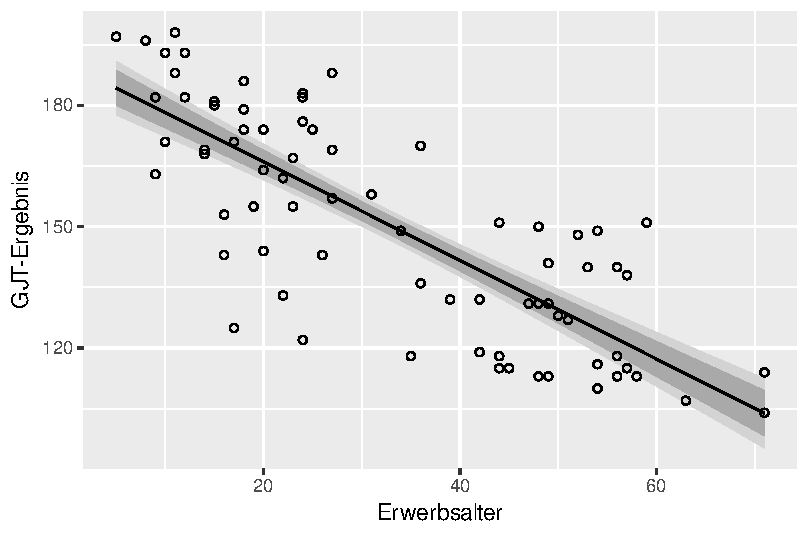
\includegraphics[width=.7\textwidth]{figs/unnamed-chunk-221-1} 

}

\caption{Regressionsgerade mit 80\%- und 95\%-Konfidenzbändern, die mittels Bootstrapping berechnet wurden.\label{fig:btstrpconfidenceband}}\label{fig:unnamed-chunk-221}
\end{figure}

\end{knitrout}

\paragraph{Identisch und unabhängig verteilte Restfehler.}
 Beim Einschätzen der Unsicherheit in den Parameterschätzungen
 und in der Regressionsgeraden haben wir eine grundlegende Annahme
 gemacht, die bisher noch nicht diskutiert wurde.
 Beim Bootstrappen haben wir auf der Basis der beobachteten
 Residuen zufällig neue Vektoren mit Residuen ($\widehat{\varepsilon}^{*}$) generiert
 und diese dann mit den $\widehat{y}$-Werten kombiniert.
 Dieser Schritt ist nur verteidigbar, wenn zwei Bedingungen gleichzeitig
 erfüllt sind:
 \begin{enumerate}
 \item Die Verteilung des Restfehler, inklusive ihre Streuung,
 ist für alle $\widehat{y}$-Werte gleich (`identisch verteilte Restfehler',
 `Homoskedastizitätsannahme'). \label{homoskedasticity}
 Zum Beispiel sollte es genauso plausibel sein, dass ein Restfehler
 von $25$ auftaucht, wenn der $\widehat{y}$-Wert $120$ ist als
 wenn er $180$ ist. Sonst wäre es ja nicht sinnvoll gewesen, die Restfehler
 beim Bootstrappen komplett zufällig durcheinander zu werfen.

 \item Die Restfehler bilden keine Klumpen. Anders gesagt, wenn wir
 den Restfehler einer bestimmten Beobachtung kennen, liefert uns
 dies nicht mehr Informationen über gewisse weitere Restfehler als über
 andere (`unabhängig verteilte Restfehler', `Unabhängigkeitsannahme').
 Wiederum wäre es sonst ja nicht
 sinnvoll gewesen, die Restfehler komplett zufällig durcheinander zu werfen,
 sondern hätten wir die Restfehler grüppchenweise neu zuordnen müssen.
 \end{enumerate}

 Ein paar Beispiele, um diese Bedingungen anschaulicher zu machen:
 \begin{itemize}
 \item Es kann durchaus vorkommen, dass die Streuung um die Regressionsgerade
 systematisch zu- oder abnimmt für grössere $\widehat{y}$-Werte. Abbildung
 \vref{fig:heteroskedasticity} zeigt zwei klare Beispiele.

 \item Jemand möchte die durchschnittliche Länge von [i]-Produktionen
 von Bernern schätzen und wählt zufällig 25 Berner aus. (So weit, so gut.)
 Jeder Sprecher liest 50 Wörter mit einem [i:] vor.
 Die Vokallängen eines beliebigen Sprechers sind sich aber denkbar ähnlicher
 als die Vokallängen unterschiedlicher Sprecher: Manche Sprecher werden
 eher überdurchschnittlich lange Vokale produzieren, manche eher unterdurchschnittlich.
 Die Restfehler (`über-/unterdurchschnittlich') der einzelnen Produktionen
 sind also nicht unabhängig voneinander, sondern bilden pro Sprecher Klumpen.

 \item Ausserdem ist es wahrscheinlich, dass das [i:] in bestimmten
 phonologischen Kontexten unterschiedlich schnell ausgesprochen wird. Die
 Restfehler bilden also auch pro phonologischen Kontext (oder pro Wort) Klumpen.
 \end{itemize}

 Wenn die sogenannte `i.i.d.'-Bedingung (\textit{identically and independently distributed})
 nicht erfüllt ist, dann ist es möglich, dass es effizientere
 Arten und Weisen gibt, um die Modellparameter zu schätzen.
 Damit ist Folgendes gemeint: Wenn Regressionsparameter mit
 der Methode der kleinsten Quadrate geschätzt werden, dann
 sind diese Schätzungen weder tendenziell Überschätzungen
 noch tendenziell Unterschätzungen---die Schätzungen
 sind also unverzerrt. Es gibt aber auch andere Methoden,
 um diese Parameter unverzerrt zu schätzen.\footnote{Um einzusehen, dass es
 vorkommen kann, dass zwei Methoden beide unverzerrte aber unterschiedliche Schätzungen
 liefern, kann man sich die folgende Methode überlegen, um das Mittel einer Stichprobe
 zu schätzen: Berechne das Stichprobenmittel wie gehabt und addiere bzw.\ subtrahiere
 mit einer Wahrscheinlickheit von jeweils 50\% 1'000 Einheiten zum bzw.\ vom Mittel.
 Das Resultat ist ebenfalls eine unverzerrte Schätzung des Populationsmittels,
 da sich die +1'000 und -1'000 über viele Stichproben hinweg ja ausgleichen.}
 Wenn die `i.i.d.'-Bedingung erfüllt, ist es ausserdem so,
 dass die Methode der kleinsten Quadrate Schätzungen liefert,
 die von Stichprobe zu Stichprobe am wenigsten voneinander
 abweichen. Ist die `i.i.d.'-Bedingung nicht erfüllt,
 dann ist es möglich, dass eine andere unverzerrte Schätzungsmethode
 Schätzungen liefert, die von Stichprobe zu Stichprobe weniger
 variieren.

 Wichtiger ist aber, dass die Schätzung der Unsicherheit betroffen ist.
 Insbesondere bei einer Verletzung der Unabhängigkeitsannahme wird die Unsicherheit
 in den Parameterschätzungen unterschätzt. Dies gilt nicht nur beim Bootstrappen,
 sondern auch beim Verwenden des zentralen Grenzwertzsatzes oder von $t$-Verteilungen.
 Im Beispiel mit den [i:] könnten wir also nicht den Standardfehler
 der durchschnittlichen Vokallänge berechnen, indem wir die Streuung in den
 Produktionen teilen durch die Wurzel von 1'250 ($25 \cdot 50$).

 Typische Verletzungen der Unabhängigkeitsannahme können
 mit sog.\ gemischten Modellen behoben werden; siehe
 Kapitel \ref{ch:weiterbildung} für Literaturvorschläge.
 Für Verletzungen der Homoskedastizitätsannahme bieten sich
 eine andere Erweiterung des linearen Modells an (siehe \citealp{Zuur2009}).
 Eine alternative Lösung ist, den Bootstrap anders durchzuführen
 (siehe \citealp[][Abschnitt 9.5]{Efron1993}).
 Aber der wichtigste Grund, weshalb wir überhaupt den Bootstrap verwenden,
 ist, um die traditionellere Methoden besser zu verstehen, und diese
 angepassten Bootstraps sind für diesen Zweck weniger geeignet.

\begin{knitrout}
\definecolor{shadecolor}{rgb}{0.969, 0.969, 0.969}\color{fgcolor}\begin{figure}[tp]

{\centering 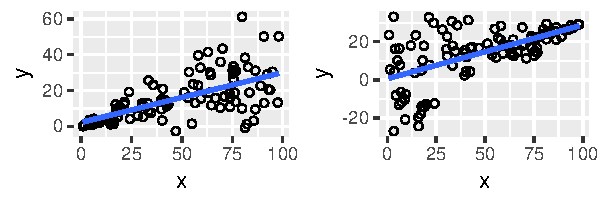
\includegraphics[width=.7\textwidth]{figs/unnamed-chunk-222-1} 

}

\caption{Die Streuung in beiden Streudiagrammen variiert erheblich je nach dem $x$- oder $\widehat{y}$-Wert.\label{fig:heteroskedasticity}}\label{fig:unnamed-chunk-222}
\end{figure}

\end{knitrout}

\subsubsection{Bootstrappen unter der Normalitätsannahme}
Wenn wir annehmen wollen, dass die Residuen nicht nur
identisch und unabhängig, sondern auch noch normalverteilt sind,
können wir die $\widehat{\varepsilon}^{*}$-Vektoren auch mit der \texttt{rnorm()}-Funktion
generieren. Das Vorgehen ist komplett analog zu dem
in Abschnitt \vref{semiparametricbootstrap} beschriebenen.
Unsere Annahmen können expliziter gemacht werden:
\begin{align}\label{eq:annahmeregression}
 y_i &= \beta_0 + \beta_1 x_i + \varepsilon_i,\\
 \varepsilon_i &\sim N(0, \sigma_{\varepsilon}^2).\nonumber
\end{align}

Der neue Teil $\varepsilon_i \sim N(0, \sigma_{\varepsilon}^2)$ macht klar,
dass wir annehmen, dass die Restfehler aus einer Normalverteilung
mit Mittel 0 und Varianz $\sigma_{\varepsilon}^2$ stammen.
$\sigma_{\varepsilon}^2$ ist ein einziger (obgleich unbekannter) Wert, sodass klar ist,
dass wir davon ausgehen, dass die Streuung der Residuen nicht von $x$
(und somit $\widehat{y}$ abhängt). Sowohl die Unabhängigkeits- als
auch die Homoskedastizitätsannahme werden von dieser Annahme umfasst.

$\sigma_{\varepsilon}$ ist zwar unbekannt, aber wird anhand der Stichprobe geschätzt;
siehe Gleichung \vref{eq:sigmap}. Der folgende Code zeigt, wie die Bootstrapschätzungen
des Schnittpunkts und der Steigung berechnet werden können. Abgesehen
von der Konstruktion der $\widehat{\varepsilon}^{*}$-Vektoren ist die Herangehensweise
aber identisch zu jener des Bootstraps ohne die Normalitätsannahme
aus dem letzten Abschnitt, sodass die anderen Schritte hier nicht mehr wiederholt werden.
\begin{knitrout}
\definecolor{shadecolor}{rgb}{0.969, 0.969, 0.969}\color{fgcolor}\begin{kframe}
\begin{alltt}
\hlstd{> }\hlstd{runs} \hlkwb{<-} \hlnum{20000}
\hlstd{> }
\hlstd{> }\hlstd{bs_beta} \hlkwb{<-} \hlkwd{matrix}\hlstd{(}\hlkwc{nrow} \hlstd{= runs,} \hlkwc{ncol} \hlstd{=} \hlnum{2}\hlstd{)}
\hlstd{> }
\hlstd{> }\hlkwa{for} \hlstd{(i} \hlkwa{in} \hlnum{1}\hlopt{:}\hlstd{runs) \{}
\hlstd{+ }  \hlcom{# Residuen aus Normalverteilung generieren}
\hlstd{+ }  \hlstd{bs_residuals} \hlkwb{<-} \hlkwd{rnorm}\hlstd{(}\hlkwc{n} \hlstd{=} \hlkwd{length}\hlstd{(}\hlkwd{resid}\hlstd{(aoa.lm)),} \hlcom{# hier: 76}
\hlstd{+ }                        \hlkwc{mean} \hlstd{=} \hlnum{0}\hlstd{,}
\hlstd{+ }                        \hlkwc{sd} \hlstd{=} \hlkwd{sigma}\hlstd{(aoa.lm))}

\hlstd{+ }  \hlstd{bs_GJT} \hlkwb{<-} \hlkwd{predict}\hlstd{(aoa.lm)} \hlopt{+} \hlstd{bs_residuals}
\hlstd{+ }  \hlstd{resampled.lm} \hlkwb{<-} \hlkwd{lm}\hlstd{(bs_GJT} \hlopt{~} \hlstd{d}\hlopt{$}\hlstd{AOA)}
\hlstd{+ }  \hlstd{bs_beta[i, ]} \hlkwb{<-} \hlkwd{coef}\hlstd{(resampled.lm)}
\hlstd{+ }\hlstd{\}}
\end{alltt}
\end{kframe}
\end{knitrout}

\subsubsection{Mit $t$-Verteilungen}\label{sec:aoa}
Wenn wir ohnehin davon ausgehen, dass die Residuen
(i.i.d.) normalverteilt sind, können wir den Standardfehler,
die Konfidenzintervalle und das Konfidenzband auch algebraisch
anhand der $t$-Verteilungen berechnen. Dadurch wird auch
die Unterschätzung von $\sigma_{\varepsilon}$ durch $\widehat{\sigma_{\varepsilon}}$
mitberücksichtigt. Bei 76 Beobachtungen und bloss zwei Parameterschätzungen
wird diese Unterschätzung aber kaum merkbar sein.
\begin{knitrout}
\definecolor{shadecolor}{rgb}{0.969, 0.969, 0.969}\color{fgcolor}\begin{kframe}
\begin{alltt}
\hlstd{> }\hlkwd{summary}\hlstd{(aoa.lm)}\hlopt{$}\hlstd{coefficients}
\end{alltt}
\begin{verbatim}
              Estimate Std. Error   t value     Pr(>|t|)
(Intercept) 190.408634  3.9040275  48.77236 5.209293e-58
AOA          -1.217977  0.1051385 -11.58450 2.728150e-18
\end{verbatim}
\end{kframe}
\end{knitrout}

\begin{knitrout}
\definecolor{shadecolor}{rgb}{0.969, 0.969, 0.969}\color{fgcolor}\begin{kframe}
\begin{alltt}
\hlstd{> }\hlcom{# 95%-Konfidenzintervalle nach t-Methode}
\hlstd{> }\hlkwd{confint}\hlstd{(aoa.lm,} \hlkwc{level} \hlstd{=} \hlnum{0.95}\hlstd{)}
\end{alltt}
\begin{verbatim}
                2.5 %     97.5 %
(Intercept) 182.62969 198.187578
AOA          -1.42747  -1.008484
\end{verbatim}
\end{kframe}
\end{knitrout}

Mit \texttt{geom\_smooth()} können $t$-basierte Konfidenzbänder
sofort gezeichnet werden, siehe Abbildung \ref{fig:geomsmooth}.
\begin{knitrout}
\definecolor{shadecolor}{rgb}{0.969, 0.969, 0.969}\color{fgcolor}\begin{kframe}
\begin{alltt}
\hlstd{> }\hlkwd{ggplot}\hlstd{(}\hlkwc{data} \hlstd{= d,}
\hlstd{+ }       \hlkwd{aes}\hlstd{(}\hlkwc{x} \hlstd{= AOA,}
\hlstd{+ }           \hlkwc{y} \hlstd{= GJT))} \hlopt{+}
\hlstd{+ }  \hlkwd{geom_point}\hlstd{(}\hlkwc{shape} \hlstd{=} \hlnum{1}\hlstd{)} \hlopt{+}
\hlstd{+ }  \hlkwd{geom_smooth}\hlstd{(}\hlkwc{method} \hlstd{=} \hlstr{"lm"}\hlstd{,} \hlkwc{level} \hlstd{=} \hlnum{0.95}\hlstd{,}
\hlstd{+ }              \hlkwc{fill} \hlstd{=} \hlstr{"red"}\hlstd{,} \hlkwc{col} \hlstd{=} \hlstr{"black"}\hlstd{)} \hlopt{+}
\hlstd{+ }  \hlkwd{geom_smooth}\hlstd{(}\hlkwc{method} \hlstd{=} \hlstr{"lm"}\hlstd{,} \hlkwc{level} \hlstd{=} \hlnum{0.67}\hlstd{,}
\hlstd{+ }              \hlkwc{fill} \hlstd{=} \hlstr{"darkred"}\hlstd{,} \hlkwc{col} \hlstd{=} \hlnum{NA}\hlstd{)}
\end{alltt}
\end{kframe}\begin{figure}[tp]

{\centering 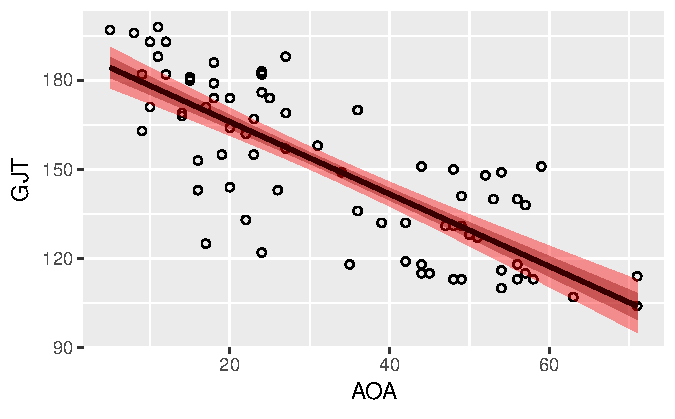
\includegraphics[width=.7\textwidth]{figs/unnamed-chunk-226-1} 

}

\caption{Regressionsgerade mit 67\%- und 95\%-Konfidenzband. Konfidenzbänder von Regressionsmodellen sind übrigens am schmalsten beim durchschnittlichen x-Wert.\label{fig:geomsmooth}}\label{fig:unnamed-chunk-226}
\end{figure}

\end{knitrout}

\section{Regressionsgeraden interpretieren}\label{sec:regressioninterpretieren}
Gleichung \vref{eq:annahmeregression} ist nützlich, um
die konzeptuelle Interpretation der Regressionsgeraden zu
verstehen.
Nach dieser Gleichung gehen wir davon aus, dass die Restfehler
zufällig (und `i.i.d.') aus einer Verteilung mit Mittel 0 stammen.
Wenn wir unsere Stichprobe als Zufallsstichprobe aus einer Population
auffassen, gehen wir also davon aus, dass in dieser Population
die $y$-Werte für jeden $x$-Werte normalverteilt sind.
% Wenn wir unsere Daten eher als Ergebnis eines datengenerierenden
% Mechanismus auffassen wollen, gehen wir davon aus, dass
% Wir gehen davon aus, dass in der Population, die
% von Interesse ist, die $y$-Werte für jeden $x$-Wert normalverteilt sind.
Folglich liegen auf der Geraden $\beta_0 + \beta_1 x_i$ die
Mittel der $y$-Verteilung \textbf{konditionell} auf $x$.
Abbildung \ref{fig:conditionalmean} stellt dieses Konzept grafisch dar.
Die geschätzte Regressionsgerade stellt also die auf Basis der
Stichprobe geschätzten konditionellen Mittel von $y$ dar,
während der Querschnitt des 95\%-Konfidenzbands an einem bestimmten
$x$-Wert das 95\%-Konfidenzintervall des $y$-Mittels für diesen $x$-Wert darstellt.

\begin{knitrout}
\definecolor{shadecolor}{rgb}{0.969, 0.969, 0.969}\color{fgcolor}\begin{figure}[tp]

{\centering 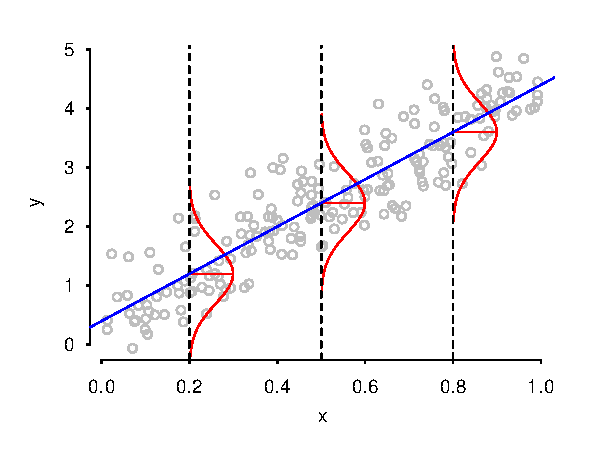
\includegraphics[width=.8\textwidth]{figs/unnamed-chunk-227-1} 

}

\caption{Wenn wir davon ausgehen, dass die Residuen i.i.d. verteilt sind, verbindet die Regressionsgerade die Mittel der $y$-Verteilungen für die unterschiedlichen $x$-Werte (`konditionelles Mittel'). In dieser Grafik sind die Residuen normalverteilt, aber dies ist keine Voraussetzung. Wenn die Residuen nicht normalverteilt sind, ist es jedoch möglich, dass das Mittel kein sehr relevantes Mass ist.\label{fig:conditionalmean}}\label{fig:unnamed-chunk-227}
\end{figure}

\end{knitrout}

Beispiele:
\begin{itemize}
 \item Laut dem \texttt{aoa.lm}-Modell sind die geschätzten
 $\beta$-Parameter $190.4$ und $-1.22$. Laut dem Modell ist
 die beste Schätzung der durchschnittlichen (Mittel) GJT-Leistung
 von Versuchspersonen mit einem AOA von 15 also $190.4 - 1.22 \cdot 15 = 172.1$.
 Dieses Ergebnis erhält man auch mit \texttt{predict()}:
\begin{knitrout}
\definecolor{shadecolor}{rgb}{0.969, 0.969, 0.969}\color{fgcolor}\begin{kframe}
\begin{alltt}
\hlstd{> }\hlkwd{predict}\hlstd{(aoa.lm,} \hlkwc{newdata} \hlstd{=} \hlkwd{tibble}\hlstd{(}\hlkwc{AOA} \hlstd{=} \hlnum{15}\hlstd{))}
\end{alltt}
\begin{verbatim}
      1 
172.139 
\end{verbatim}
\end{kframe}
\end{knitrout}
  Bemerken Sie aber, dass es in unserem Datensatz zwei Versuchspersonen
  mit einem AOA von 15 gibt und dass ihr Durchschnittsergebnis nicht 172.1 ist:
\begin{knitrout}
\definecolor{shadecolor}{rgb}{0.969, 0.969, 0.969}\color{fgcolor}\begin{kframe}
\begin{alltt}
\hlstd{> }\hlstd{d |>} \hlkwd{filter}\hlstd{(AOA} \hlopt{==} \hlnum{15}\hlstd{)}
\end{alltt}
\begin{verbatim}
# A tibble: 2 x 2
    AOA   GJT
  <dbl> <dbl>
1    15   180
2    15   181
\end{verbatim}
\end{kframe}
\end{knitrout}
Inwiefern unsere modellbasierte Schätzung eine zuverlässigere Schätzung des
konditionellen Mittels darstellt als das Mittel dieser beiden Werte, hängt
von der Gültigkeit unserer Annahmen ab. Die Annahme eines linearen Zusammenhangs
scheint hier doch auf jeden Fall nicht wahnsinnig daneben zu liegen.
Konzeptuell gesprochen erlaubt uns diese Annahme,
$y$-Mittel für bestimmte $x$-Werte besser zu schätzen,
indem wir auch Information über den $x$--$y$-Zusammenhang,
die wir aus den restlichen Daten ableiten, mit einbeziehen.

 \item Versuchspersonen mit einem AOA von 21 gibt es in der Stichprobe
 nicht. Nach der Regressionsgleichung wäre aber das Durchschnittsergebnis
 von Versuchspersonen mit diesem AOA in der Population etwa 165 Punkte.
\begin{knitrout}
\definecolor{shadecolor}{rgb}{0.969, 0.969, 0.969}\color{fgcolor}\begin{kframe}
\begin{alltt}
\hlstd{> }\hlkwd{predict}\hlstd{(aoa.lm,} \hlkwc{newdata} \hlstd{=} \hlkwd{tibble}\hlstd{(}\hlkwc{AOA} \hlstd{=} \hlnum{21}\hlstd{))}
\end{alltt}
\begin{verbatim}
       1 
164.8311 
\end{verbatim}
\end{kframe}
\end{knitrout}

  Dies ist ein Beispiel von \textbf{Intrapolation}, denn
  es gibt sowohl Versuchspersonen mit niedrigeren als mit höheren AOA-Werten
  in der Stichprobe.

 \item Versuchspersonen mit einem AOA von 82 gibt es in der Stichprobe auch
 nicht. Nach der Regressionsgleichung wäre aber das Durchschnittsergebnis
 von Versuchspersonen mit diesem AOA in der Population etwa 91 Punkte.
\begin{knitrout}
\definecolor{shadecolor}{rgb}{0.969, 0.969, 0.969}\color{fgcolor}\begin{kframe}
\begin{alltt}
\hlstd{> }\hlkwd{predict}\hlstd{(aoa.lm,} \hlkwc{newdata} \hlstd{=} \hlkwd{tibble}\hlstd{(}\hlkwc{AOA} \hlstd{=} \hlnum{82}\hlstd{))}
\end{alltt}
\begin{verbatim}
       1 
90.53455 
\end{verbatim}
\end{kframe}
\end{knitrout}

  Dies ist ein Beispiel von \textbf{Extrapolation}, denn
  das Maximumalter in der Stichprobe ist 71 Jahre.

  \item Das durchschnittliche (Mittel) AOA in der Stichprobe ist etwa 32.5 Jahre.
  Das geschätzte konditionelle GJT-Mittel für dieses Alter ist gleich dem Mittel
  der Stichprobe.
\begin{knitrout}
\definecolor{shadecolor}{rgb}{0.969, 0.969, 0.969}\color{fgcolor}\begin{kframe}
\begin{alltt}
\hlstd{> }\hlkwd{predict}\hlstd{(aoa.lm,} \hlkwc{newdata} \hlstd{=} \hlkwd{tibble}\hlstd{(}\hlkwc{AOA} \hlstd{=} \hlkwd{mean}\hlstd{(d}\hlopt{$}\hlstd{AOA)))}
\end{alltt}
\begin{verbatim}
       1 
150.7763 
\end{verbatim}
\end{kframe}
\end{knitrout}
  Dies ist natürlich kein Zufall, sondern ein allgemeines Phänomen.
  Wenn wir Gleichung \ref{eq:intercept} in die Regressiongleichung
  einsetzen, erhalten wir ja Folgendes:
  $$\widehat{y_i} = \underbrace{\bar{y} - \widehat{\beta_1} \bar{x}}_{= \widehat{\beta_0}} +  \widehat{\beta_1}x_i.$$
  Für $x_i = \bar{x}$ erhalten wir also $\widehat{y_i} = \bar{y}$.

  \item Konfidenzintervalle um konditionelle Mittel können
  mit den oben beschriebenen Bootstrapmethoden berechnet werden,
  indem man das `Konfidenzband' für nur einen $x$-Wert berechnet.
  Man kann aber auch \texttt{predict()} verwenden; dann wird
  das Konfidenzintervall auf der Basis der geeigneten $t$-Verteilung
  konstruiert.

\begin{knitrout}
\definecolor{shadecolor}{rgb}{0.969, 0.969, 0.969}\color{fgcolor}\begin{kframe}
\begin{alltt}
\hlstd{> }\hlkwd{predict}\hlstd{(aoa.lm,} \hlkwc{newdata} \hlstd{=} \hlkwd{tibble}\hlstd{(}\hlkwc{AOA} \hlstd{=} \hlnum{35}\hlstd{),}
\hlstd{+ }        \hlkwc{interval} \hlstd{=} \hlstr{"confidence"}\hlstd{,} \hlkwc{level} \hlstd{=} \hlnum{0.80}\hlstd{)}
\end{alltt}
\begin{verbatim}
       fit      lwr      upr
1 147.7795 145.3246 150.2343
\end{verbatim}
\end{kframe}
\end{knitrout}
\end{itemize}

\medskip

\begin{framed}
\noindent \textbf{Einschub: Extra- und Intrapolation.}
Seien Sie vorsichtig mit Extrapolation:
Wenn wir eine Stichprobe von Versuchspersonen zwischen
8 und 26 Jahren haben, ist es gefährlich, Aussagen über 5- oder 40-Jährige zu machen.
 Dies wird in der linken Abbildung illustriert:
 Eine Fähigkeit, die sich im Alter zwischen 10 und 35 entwickelt, hat nicht unbedingt die gleiche Entwicklung ausserhalb dieses Bereichs.
 Eine Extrapolierung auf der Basis der Regressionsgeraden ist hier irreführend.
 Auch bei Intrapolation ist Vorsicht geboten.
 Aus den Daten in der rechten Grafik könnte man zum Beispiel die Schlussfolgerung ziehen,
 dass sich Reaktionszeiten im Alter graduell verlängern.
 Auch diese Schlussfolgerung dürfte zu kurz greifen.

\begin{knitrout}
\definecolor{shadecolor}{rgb}{0.969, 0.969, 0.969}\color{fgcolor}

{\centering 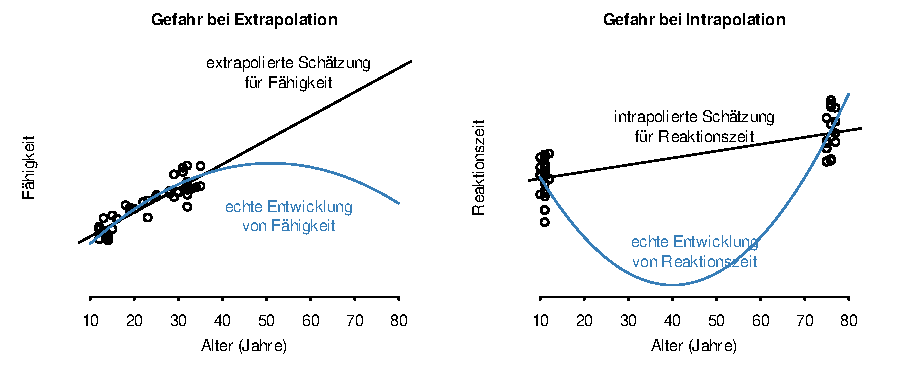
\includegraphics[width=.9\textwidth]{figs/unnamed-chunk-234-1} 

}


\end{knitrout}
\end{framed}

\medskip

\paragraph{Den Schnittpunkt interpretierbarer machen.}
Der geschätzte Schnittpunkt hat nicht unbedingt eine nützliche
Interpretation. In unserem Fall stellt er die geschätzte Durchschnittsleistung
von Versuchspersonen mit AOA 0 dar. Solche gibt es in der Stichprobe
nicht, sodass diese Zahl eine Art Extrapolation darstellt.
Sie können den Schnittpunkt interpretierbarer machen, indem
Sie das Stichprobenmittel des Prädiktors von den Prädiktorwerten
abziehen und mit diesen neuen Werten arbeiten.
Diese Technik heisst \textbf{zentrieren} (\textit{centring}).
Ein Vorteil des Zentrierens ist, dass der geschätzte Schnittpunkt
einem jetzt sofort auch sagt, was das Stichprobenmittel der $y$-Variable ist.

\begin{knitrout}
\definecolor{shadecolor}{rgb}{0.969, 0.969, 0.969}\color{fgcolor}\begin{kframe}
\begin{alltt}
\hlstd{> }\hlcom{# AOA zentrieren}
\hlstd{> }\hlstd{d}\hlopt{$}\hlstd{c.AOA} \hlkwb{<-} \hlstd{d}\hlopt{$}\hlstd{AOA} \hlopt{-} \hlkwd{mean}\hlstd{(d}\hlopt{$}\hlstd{AOA)}
\hlstd{> }
\hlstd{> }\hlcom{# Modell neu fitten}
\hlstd{> }\hlstd{aoa.lm} \hlkwb{<-} \hlkwd{lm}\hlstd{(GJT} \hlopt{~} \hlstd{c.AOA,} \hlkwc{data} \hlstd{= d)}
\hlstd{> }
\hlstd{> }\hlcom{# Parameterschätzungen}
\hlstd{> }\hlkwd{summary}\hlstd{(aoa.lm)}\hlopt{$}\hlstd{coefficients}
\end{alltt}
\begin{verbatim}
              Estimate Std. Error   t value     Pr(>|t|)
(Intercept) 150.776316  1.8807316  80.16897 1.120538e-73
c.AOA        -1.217977  0.1051385 -11.58450 2.728150e-18
\end{verbatim}
\end{kframe}
\end{knitrout}

Achten Sie aber darauf, dass eine Versuchsperson mit einem AOA
von 35 jetzt für das Modell eine Versuchsperson mit einem \texttt{c.AOA}
von $35 - \bar{x}_{AOA} = 2.46$ ist:
\begin{knitrout}
\definecolor{shadecolor}{rgb}{0.969, 0.969, 0.969}\color{fgcolor}\begin{kframe}
\begin{alltt}
\hlstd{> }\hlkwd{predict}\hlstd{(aoa.lm,} \hlkwc{newdata} \hlstd{=} \hlkwd{tibble}\hlstd{(}\hlkwc{c.AOA} \hlstd{=} \hlnum{35} \hlopt{-} \hlkwd{mean}\hlstd{(d}\hlopt{$}\hlstd{AOA)),}
\hlstd{+ }        \hlkwc{interval} \hlstd{=} \hlstr{"confidence"}\hlstd{,} \hlkwc{level} \hlstd{=} \hlnum{0.80}\hlstd{)}
\end{alltt}
\begin{verbatim}
       fit      lwr      upr
1 147.7795 145.3246 150.2343
\end{verbatim}
\end{kframe}
\end{knitrout}

\section{Modellannahmen überprüfen}
Die Modellresiduen sollten grafisch dargestellt werden, um
die Modellannahmen zu überprüfen. Leitfragen dabei sind
unter anderem:
\begin{itemize}
	\item Gibt es noch einen erkennbaren Zusammenhang zwischen
	      den Residuen und den $\widehat{y}$-Werten? Ein
	      solcher Zusammenhang deutet darauf hin, dass der
	      Zusammenhang zwischen einem oder mehreren Prädiktoren
	      und dem outcome nicht-linear ist.

	\item Variiert die Streuung der Residuen mit $\widehat{y}$
	      oder mit den Prädiktoren? Systematische Unterschiede
	      in der Streuung der Residuen deuten darauf hin, dass
	      der Restfehler `heteroskedastisch' ist.

	\item Sind die Residuen ungefähr normalverteilt? Nicht-normalverteilte
        Residuen lassen vermuten, dass die Annahme, dass der Restfehler
        aus einer Normalverteilung stammt, nicht stimmt. Dies hätte einerseits
        Konsequenzen für die auf $t$-Verteilungen basierten Konfidenzintervalle
        und Konfidenzbänder. Andererseits, und wichtiger,
        sind die konditionellen Mittel, die
        die Regressionslinie darstellt, eventuell weniger relevant.

	\item Gibt es einzelne Datenpunkte, die einen viel stärkeren
        Einfluss aufs Regressionsmodell ausüben als die meisten?
        Das Problem mit einflussreichen Datenpunkten ist,
        dass sie etwa dazu führen können, dass das Modell
        einen leichten positiven Zusammenhang zwischen den Variablen
        findet, während für die meisten Datenpunkte ein starker
        negativer Zusammenhang vorliegt.
\end{itemize}

Abbildung \ref{fig:modeldiagnostics} zeigt ein paar nützliche
Grafiken, die man einfach mit \texttt{plot(aoa.lm)} generieren
kann. Auf riesige Probleme in den Modellannahmen deuten diese
Grafiken m.E.\ nicht hin. (Solche Probleme würde man ohnehin
nicht erwarten, wenn man sich das Streudiagramm am Anfang dieses
Kapitels angeschaut hat. In meiner Erfahrung stösst man selten
auf Überraschungen, wenn man die Daten bereits ausführlich
grafisch dargestellt hat.)
\begin{knitrout}
\definecolor{shadecolor}{rgb}{0.969, 0.969, 0.969}\color{fgcolor}\begin{figure}[tp]

{\centering \includegraphics[width=.66\textwidth]{figs/unnamed-chunk-237-1} 

}

\caption{Grafische Modelldiagnose des \texttt{aoa.lm}-Modells mithilfe der \texttt{plot()}-Funktion. \textit{Links oben:} Zusammenhang zwischen Residuen und $\widehat{y}$. Die rote Trendlinie sollte ungefähr flach sein. Sonstige auffällige Muster wären auch unerwünscht. \textit{Rechts oben:} Normalität der Residuen. Wenn die Residuen normalverteilt sind, liegen sie auf der gestrichelten Diagonale. \textit{Links unten:} Streuung in den Residuen. Eine flache rote Trendlinie deutet auf Homoskedastizität hin. \textit{Rechts unten:} Manchmal gibt es in dieser Grafik ein paar gestrichelte rote Linien. Datenpunkte, die jenseits dieser Linien liegen, dürften viel einflussreicher als andere Datenpunkte sein.\label{fig:modeldiagnostics}}\label{fig:unnamed-chunk-237}
\end{figure}

\end{knitrout}

\begin{knitrout}
\definecolor{shadecolor}{rgb}{0.969, 0.969, 0.969}\color{fgcolor}\begin{kframe}
\begin{alltt}
\hlstd{> }\hlcom{# 4 Grafiken in 2x2-Raster zeichnen.}
\hlstd{> }\hlcom{# (Dies funktioniert nicht für ggplot!)}
\hlstd{> }\hlkwd{par}\hlstd{(}\hlkwc{mfrow} \hlstd{=} \hlkwd{c}\hlstd{(}\hlnum{2}\hlstd{,} \hlnum{2}\hlstd{))}
\hlstd{> }\hlcom{# Modelldiagnosen darstellen}
\hlstd{> }\hlkwd{plot}\hlstd{(aoa.lm)}
\hlstd{> }\hlcom{# Ab jetzt wieder normal zeichnen.}
\hlstd{> }\hlkwd{par}\hlstd{(}\hlkwc{mfrow} \hlstd{=} \hlkwd{c}\hlstd{(}\hlnum{1}\hlstd{,} \hlnum{1}\hlstd{))}
\end{alltt}
\end{kframe}
\end{knitrout}


Aufgrund des Stichprobenfehlers wird man oft---rein durch
Zufall---Zusammenhänge und nicht-normalverteilte Residuen
finden, sodass man ein bisschen Erfahrung braucht, um
unbedeutende Muster in den Residuen von potenziellen
Problemen zu unterscheiden. Ausserdem sind Modellannahmen
gerade bei kleineren Stichproben schwieriger zu überprüfen.
Für mehr Informationen hierzu, siehe \href{https://janhove.github.io/analysis/2018/04/25/graphical-model-checking}{\textit{Checking model assumptions without getting paranoid}} (25.4.2018)
und \citet{Vanhove2018b}.
Siehe ausserdem
\href{https://janhove.github.io/analysis/2019/04/11/assumptions-relevance}{\textit{Before worrying about model assumptions, think about model relevance}} (11.4.2019).

Das Thema Modellkritik wird weiter behandelt von
unter anderem
\citet{Baayen2008},
\citet[][Kapitel 4]{Cohen2003},
\citet[][Kapitel 4]{Faraway2005},
\citet[][Kapitel 8--9]{Weisberg2005} und
\citet[][Kapitel 2]{Zuur2009}.
Statt sich zu sehr in technischen Details zu verlieren,
halte ich es aber sinnvoller, sich stets die Relevanzfrage
zu stellen (vgl.\ Blogeintrag 11.4.2019).

\paragraph{Aufgabe.} Obwohl die Modelldiagnose
nicht auf grössere Probleme hindeutet, können
die Modellannahmen eigentlich gar nicht stimmen.
Erklären Sie.

\section{Aufgaben}

\begin{enumerate}
 \item Führen Sie folgende Analyse auf die \texttt{dekeyser2010.csv}-Daten aus:
\begin{knitrout}
\definecolor{shadecolor}{rgb}{0.969, 0.969, 0.969}\color{fgcolor}\begin{kframe}
\begin{alltt}
\hlstd{> }\hlkwd{plot}\hlstd{(AOA} \hlopt{~} \hlstd{GJT,} \hlkwc{data} \hlstd{= d)}
\hlstd{> }\hlstd{gjt.lm} \hlkwb{<-} \hlkwd{lm}\hlstd{(AOA} \hlopt{~}  \hlstd{GJT,} \hlkwc{data} \hlstd{= d)}
\hlstd{> }\hlkwd{summary}\hlstd{(gjt.lm)}
\end{alltt}
\end{kframe}
\end{knitrout}
\begin{enumerate}
\item Erklären Sie, was Sie gerade berechnet haben. Was bedeuten die geschätzten Parameter? Wieso ist das Intercept so gross?
Was bedeutet das Intercept?
\item Welches Modell finden Sie am sinnvollsten: \texttt{aoa.lm} oder \texttt{gjt.lm}? Warum?
\end{enumerate}

 \item Die Datei \texttt{vanhove2014\_cognates.csv} enthält eine Zusammenfassung der Daten meiner Dissertation
 \citep{Vanhove2014}.
 163 Deutschschweizer Versuchspersonen wurden gebeten, 45 geschriebene und 45 (andere) gesprochene
 schwedische Wörter ins Deutsche zu übersetzen. Die Anzahl richtiger Antworten steht in
 den Spalten \texttt{CorrectWritten} für geschriebene Wörter bzw.\ \texttt{CorrectSpoken} für gesprochene Wörter. Die Datei \texttt{vanhove2014\_background.csv}
 enthält Angaben zur Leistung der Versuchspersonen bei weiteren Sprach- und kognitiven Tests.
 Fügen Sie die beiden Datensätze zusammen.

 Versuchen Sie, die folgenden Fragen zu beantworten.

 \begin{enumerate}
  \item \texttt{DS.Span} enthält die Leistung der Versuchspersonen
  bei einem Arbeitsgedächtnistest.
  Wie hängt die Leistung bei \texttt{DS.Span} mit \texttt{CorrectSpoken} zusammen?

 \item Wie hängt die Leistung bei einem Englischtest
 (\texttt{English.Overall}) mit der Übersetzungsleistung
 in der geschriebenen Modalität zusammen?

 \item Wie variiert die Übersetzungsleistung in den beiden
 Modalitäten mit dem Alter (\texttt{Age}) der Versuchspersonen?
\end{enumerate}
\end{enumerate}


\chapter{Gruppenunterschiede}\label{ch:gruppenunterschiede}

Im vorigen Kapitel haben wir uns mit der Frage
beschäftigt, wie man den Zusammenhang zwischen
einem kontinuierlichen Prädiktor und einem
kontinuierlichen outcome modellieren kann.
In diesem Kapitel widmen wir uns der Frage,
wie Zusammenhänge zwischen \textbf{kategorischen}
Prädiktoren und einem kontinuierlichen outcome
modelliert werden können. Das typische Beispiel
eines kategorischen Prädiktors ist die Kondition in einem Experiment:
Wie stark unterscheiden sich die Ergebnisse von Teilnehmenden
in der Experimentalgruppe im Schnitt von jenen von Teilnehmenden
in der Kontrollgruppe? Das Vorgehen ist nahezu identisch
mit dem aus dem letzten Kapitel.

\section{Unterschiede zwischen zwei Gruppen}
Das Beispiel, dem wir uns hier widmen, stammt nicht aus der
Sprachwissenschaft, sondern aus der Sozialpsychologie.
\citet[][Experiment 1]{Caruso2013} berichteten, dass
amerikanische Versuchspersonen Aussagen, die das US-amerikanische
Sozialsystem rechtfertigen, stärker zustimmen, wenn
man sie an Geld erinnert (sogenanntes \textit{currency priming}).
Ihr Design sah wie folgt aus. Es gab acht Aussagen im Stil von
\textit{Everyone has a fair shot at wealth and happiness}.
Die Teilnehmenden deuteten am Bildschirm
ihre Zustimmung zu diesen Aussagen
auf einer 7-stufigen Likertskala an (1 = überhaupt nicht einverstanden,
7 = vollständig einverstanden). Pro Versuchsperson wurden
die acht Zustimmungswerte gemittelt.
Die Hälfte der Versuchspersonen sah im Hintergrund ein verblasstes
aber ersichtliches Bild einer Banknote; bei der anderen Hälfte
war dieses Bild verwischt.
Die Versuchspersonen, welche die Banknote im Hintergrund sahen,
stimmten den Aussagen stärker zu, als jene, bei denen das Bild
verwischt war.
\citet{Klein2014} versuchten, dieses Ergebnis in 36 neuen
Stichproben zu replizieren.
In der Datei \texttt{Klein2014\_money\_abington.csv} finden Sie
die Ergebnisse einer dieser Stichproben (84 Teilnehmende).
Diese Daten werden wir analysieren.

\paragraph{Aufgabe.} Lesen Sie diese Datei in R ein.
Den Datensatz können Sie einfach \texttt{d} nennen.
Vergessen Sie nicht zu kontrollieren, ob das Einlesen
geklappt hat.



\subsection{Grafische Darstellung: Boxplots}
Eine nützliche grafische Darstellung, um unterschiedliche
Gruppen hinsichtlich eines mehr oder weniger kontinuierlichen
outcomes zu vergleichen, ist der Boxplot
(zu Deutsch auch \textit{Kastengrafik}).
Abbildung \ref{fig:boxplot} zeigt als Beispiel
einen Boxplot der Ergebnisse bei einem Wortschatztest
der 80 Versuchspersonen von \citet{Vanhove2016}.
Die dickere Linie in der Mitte liegt beim Median
und das Kästchen reicht vom 25.\ bis zum 75.\ Perzentil
und umfasst somit die Hälfte der Datenpunkte.
Manchmal gibt es (wie hier) auch Kreischen in einem Boxplot.
Diese stellen Extremwerte dar, die mehr als 1.5 Mal
die Distanz zwischen dem 25.\ und dem 75.\ Perzentil
vom 25.\ oder 75.\ Perzentil entfernt liegen.
Diese Extremwerte sind mögliche (!) Ausreisser.
Mit einem Dotplot kann man besser überprüfen, ob sie tatsächlich
auch Ausreisser sind. In diesem Beispiel liegen die zwei
möglichen Ausreisser nicht sehr weit von anderen Datenpunkten
entfernt, sodass sie nicht als Ausreisser gelten.

\begin{knitrout}
\definecolor{shadecolor}{rgb}{0.969, 0.969, 0.969}\color{fgcolor}\begin{figure}[tp]

{\centering \includegraphics[width=.5\textwidth]{figs/unnamed-chunk-242-1} 

}

\caption{Erklärung Boxplot.\label{fig:boxplot}}\label{fig:unnamed-chunk-242}
\end{figure}

\end{knitrout}

Mit \texttt{ggplot()} können solche Boxplots mithilfe des
\texttt{geom\_boxplot()}-Befehls erzeugt werden.
Weiter ist zu bemerken, dass wir die Grafik zunächst einmal als ein Objekt
namens \texttt{p\_boxplot} in die Arbeitsumgebung speichern.
Um die Grafik dann tatsächlich zu zeichnen, müssen wir lediglich
diesen Objektnamen eintippen.
Das Ergebnis steht in Abbildung \ref{fig:boxplotklein1}.

\begin{knitrout}
\definecolor{shadecolor}{rgb}{0.969, 0.969, 0.969}\color{fgcolor}\begin{kframe}
\begin{alltt}
\hlstd{> }\hlstd{p_boxplot} \hlkwb{<-} \hlkwd{ggplot}\hlstd{(}\hlkwc{data} \hlstd{= d,}
\hlstd{+ }                    \hlkwd{aes}\hlstd{(}\hlkwc{x} \hlstd{= MoneyGroup,}
\hlstd{+ }                        \hlkwc{y} \hlstd{= Sysjust))} \hlopt{+}
\hlstd{+ }  \hlkwd{geom_boxplot}\hlstd{()} \hlopt{+}
\hlstd{+ }  \hlkwd{xlab}\hlstd{(}\hlstr{"Kondition"}\hlstd{)} \hlopt{+}
\hlstd{+ }  \hlkwd{ylab}\hlstd{(}\hlstr{"Systemrechtfertigungsscore"}\hlstd{)}
\hlstd{> }\hlstd{p_boxplot}
\end{alltt}
\end{kframe}\begin{figure}[tp]

{\centering \includegraphics[width=.4\textwidth]{figs/unnamed-chunk-243-1} 

}

\caption{Vergleich der Systemrechtfertigungsscores in den beiden Konditionen in Klein et al.'s (2014) Replikation von Caruso et al. (2013, Experiment 1). Daten aus der Abington-Stichprobe.\label{fig:boxplotklein1}}\label{fig:unnamed-chunk-243}
\end{figure}

\end{knitrout}

Ich finde es oft eine gute Idee,
dem Boxplot auch noch die einzelnen Datenpunkte
hinzuzufügen \citep[siehe auch][]{Weissgerber2015}.
Insbesondere bei eher kleinen Datensätzen
beeinträchtigt dies die Interpretierbarkeit der Grafik nicht
und hilft es den Lesenden, einzuschätzen, wie die
Daten tatsächlich verteilt sind. Boxplots können
in dieser Hinsicht nämlich manchmal täuschen;
siehe auch \href{https://www.cedricscherer.com/2021/06/06/visualizing-distributions-with-raincloud-plots-and-how-to-create-them-with-ggplot2/}{\textit{Visualizing distributions with raincloud plots (and how to create them with ggplot2)}}
unter \url{https://www.cedricscherer.com/}.

Der Code unten zeigt Ihnen, wie Sie dies machen können.
Dem \texttt{geom\_boxplot()}-Befehl wird der Parameter
\texttt{outlier.shape = NA} übergeben, womit verhindert wird,
dass allfällige Extremwerte zwei Mal dargestellt werden: ein Mal
als Kreischen beim Boxplot und ein Mal als einzelner Datenpunkt.
Mit \texttt{geom\_point()} werden die Datenpunkte einzeln dargestellt.
Der Parameter \texttt{shape = 1} sorgt dafür, dass sie als leere Kreischen
gezeichnet werden
(siehe \texttt{?pch $\rightarrow$ `pch' values} für andere mögliche Werte).
Die Einstellung \texttt{position = position\_jitter(width = ?, height = ?)}
verschiebt die Punkte etwas horizontal und vertikal, damit überlappende
Punkte sichtbar werden. Mit den Einstellungen unten werden die Punkte
nur horizontal etwas verschoben, aber nicht vertikal.
Zu guter Letzt werden die Defaultwerte auf der x-Achse (`control' und `treatment'; siehe Abbildung \ref{fig:boxplotklein1}) mit
dem Befehl \texttt{scale\_x\_discrete()} durch `ohne' bzw.\ `mit' ersetzt.
Das Resultat zeigt Abbildung \vref{fig:boxplotklein2}.

\begin{knitrout}
\definecolor{shadecolor}{rgb}{0.969, 0.969, 0.969}\color{fgcolor}\begin{kframe}
\begin{alltt}
\hlstd{> }\hlstd{p_boxplotdeluxe} \hlkwb{<-} \hlkwd{ggplot}\hlstd{(}\hlkwc{data} \hlstd{= d,}
\hlstd{+ }                    \hlkwd{aes}\hlstd{(}\hlkwc{x} \hlstd{= MoneyGroup,}
\hlstd{+ }                        \hlkwc{y} \hlstd{= Sysjust))} \hlopt{+}
\hlstd{+ }  \hlkwd{geom_boxplot}\hlstd{(}\hlkwc{outlier.shape} \hlstd{=} \hlnum{NA}\hlstd{)} \hlopt{+}
\hlstd{+ }  \hlkwd{geom_point}\hlstd{(}\hlkwc{shape} \hlstd{=} \hlnum{1}\hlstd{,}
\hlstd{+ }             \hlkwc{position} \hlstd{=} \hlkwd{position_jitter}\hlstd{(}\hlkwc{width} \hlstd{=} \hlnum{0.2}\hlstd{,} \hlkwc{height} \hlstd{=} \hlnum{0}\hlstd{))} \hlopt{+}
\hlstd{+ }  \hlkwd{xlab}\hlstd{(}\hlstr{"Banknote"}\hlstd{)} \hlopt{+}
\hlstd{+ }  \hlkwd{scale_x_discrete}\hlstd{(}\hlkwc{labels} \hlstd{=} \hlkwd{c}\hlstd{(}\hlstr{"ohne"}\hlstd{,} \hlstr{"mit"}\hlstd{))} \hlopt{+}
\hlstd{+ }  \hlkwd{ylab}\hlstd{(}\hlstr{"Systemrechtfertigungsscore"}\hlstd{)}
\hlstd{> }\hlstd{p_boxplotdeluxe}
\end{alltt}
\end{kframe}\begin{figure}[tp]

{\centering \includegraphics[width=.5\textwidth]{figs/unnamed-chunk-244-1} 

}

\caption{Nochmals die gleichen Daten, aber mit den einzelnen Datenpunkten.\label{fig:boxplotklein2}}\label{fig:unnamed-chunk-244}
\end{figure}

\end{knitrout}

Mehr Informationen zu Befehlen wie \texttt{position\_jitter()} und \texttt{scale\_x\_discrete()} finden Sie unter \url{https://ggplot2.tidyverse.org/reference/}.
Siehe auch meinen Blogeintrag \href{https://janhove.github.io/reporting/2015/01/07/some-alternatives-to-barplots}{\textit{Some alternatives to bar plots}} (7.1.2015).

\subsection{Numerische Zusammenfassung}
Eine Tabelle mit den üblichen beschreibenden Statistiken pro Gruppe
können wir leicht mit \texttt{group\_by()} und \texttt{summarise()} herstellen.

\begin{knitrout}
\definecolor{shadecolor}{rgb}{0.969, 0.969, 0.969}\color{fgcolor}\begin{kframe}
\begin{alltt}
\hlstd{> }\hlstd{d |>}
\hlstd{+ }  \hlkwd{group_by}\hlstd{(MoneyGroup) |>}
\hlstd{+ }  \hlkwd{summarise}\hlstd{(}\hlkwc{AnzahlVpn} \hlstd{=} \hlkwd{n}\hlstd{(),}
\hlstd{+ }            \hlkwc{Mittel} \hlstd{=} \hlkwd{mean}\hlstd{(Sysjust),}
\hlstd{+ }            \hlkwc{Median} \hlstd{=} \hlkwd{median}\hlstd{(Sysjust),}
\hlstd{+ }            \hlkwc{StdAbw} \hlstd{=} \hlkwd{sd}\hlstd{(Sysjust))}
\end{alltt}
\begin{verbatim}
# A tibble: 2 x 5
  MoneyGroup AnzahlVpn Mittel Median StdAbw
  <chr>          <int>  <dbl>  <dbl>  <dbl>
1 control           44   3.53   3.56  0.781
2 treatment         40   3.53   3.94  1.02 
\end{verbatim}
\end{kframe}
\end{knitrout}


\subsection{Modellierung}\label{sec:money_model}
\subsubsection{Dummy-Variablen}
Die grafische Darstellung zeigt, dass der Median der `mit Banknote'-Kondition
zwar höher ist als jener der `ohne Banknote'-Kondition, aber das die
Überlappung zwischen beiden Konditionen erheblich ist.
Die numerische Zusammenfassung zeigt ausserdem, dass sich die Mittel kaum unterscheiden.
Trotzdem können wir diese Daten---ähnlich wie im letzten Kapitel---in ein Modell giessen.
Dieses Modell wird ebenfalls von Gleichung \vref{eq:simpleregression} beschrieben, die hier wiederholt wird:
\begin{equation}
y_i = \beta_0 + \beta_1 x_i + \varepsilon_i.
\end{equation}

$y_i$ stellt nun den Systemrechtfertigungsscore der $i$.\ Versuchsperson dar;
$x_i$ stellt die Gruppenzugehörigkeit dieser Versuchsperson dar, d.h.,
ob die Versuchsperson zu der `control'- oder `treatment'-Gruppe gehört.
Genau wie vorher müssen $\beta_0$ und $\beta_1$ (und als Konsequenz
davon auch $\varepsilon_i$) geschätzt werden.

Gleichungen wie diese können natürlich schwer mit Wörtern
wie `control' und `treatment' umgehen, aber die Lösung ist erstaunlich einfach:
Eine Gruppe bezeichnen wir als $0$ und die andere als $1$.
Zum Beispiel können wir festlegen, dass $x_i = 0$, wenn die $i$.\ Versuchsperson
zur `control'-Kondition gehört, und dass $x_i = 1$, wenn sie zur `treatment'-Kondition
gehört.\footnote{Wir könnten auch festlegen, dass $x_i = 1$ für Versuchspersonen
in der Kontrollkondition und $x_i = 0$ für Versuchspersonen in der Experimentalkondition.
Das macht eigentlich nichts aus.} Wenn wir dies gemacht haben,
können wir den Vektor von Nullen und Einsen als Prädiktor in ein lineares Regressionsmodell
aufnehmen. Wenn man kategorische Variablen (hier: Gruppenzugehörigkeit)
als Zahlenreihen umschreibt, spricht man von \textbf{Dummy-Variablen}.

Gezeigt werden hier zwei Möglichkeiten, um die Dummy-Variable \texttt{n.Kondition}
zu kreieren. Die erste funktioniert mit \texttt{ifelse()}:
\begin{knitrout}
\definecolor{shadecolor}{rgb}{0.969, 0.969, 0.969}\color{fgcolor}\begin{kframe}
\begin{alltt}
\hlstd{> }\hlcom{# n.Kondition == 1, falls MoneyGroup == "treatment"; 0, falls nicht.}
\hlstd{> }\hlstd{d}\hlopt{$}\hlstd{n.Kondition} \hlkwb{<-} \hlkwd{ifelse}\hlstd{(d}\hlopt{$}\hlstd{MoneyGroup} \hlopt{==} \hlstr{"treatment"}\hlstd{,} \hlkwc{yes} \hlstd{=} \hlnum{1}\hlstd{,} \hlkwc{no} \hlstd{=} \hlnum{0}\hlstd{)}
\end{alltt}
\end{kframe}
\end{knitrout}

Die zweite verwendet die tidyverse-Funktionen \texttt{mutate()} und \texttt{case\_when()}.
Beide Möglichkeiten liefern das gleiche Ergebnis; die Idee hier ist nur, die Funktion
\texttt{case\_when()} vorzustellen.
\begin{knitrout}
\definecolor{shadecolor}{rgb}{0.969, 0.969, 0.969}\color{fgcolor}\begin{kframe}
\begin{alltt}
\hlstd{> }\hlstd{d} \hlkwb{<-} \hlstd{d |>}
\hlstd{+ }  \hlkwd{mutate}\hlstd{(}\hlkwc{n.Kondition} \hlstd{=} \hlkwd{case_when}\hlstd{(}
\hlstd{+ }    \hlcom{# n.Kondition == 1, falls MoneyGroup == "treatment"}
\hlstd{+ }    \hlstd{MoneyGroup} \hlopt{==} \hlstr{"treatment"} \hlopt{~} \hlnum{1}\hlstd{,}
\hlstd{+ }    \hlcom{# n.Kondition == 0 sonst}
\hlstd{+ }    \hlnum{TRUE}                      \hlopt{~} \hlnum{0}
\hlstd{+ }  \hlstd{))}
\end{alltt}
\end{kframe}
\end{knitrout}

Zur Kontrolle ist eine Kreuztabelle mit der ursprünglichen und der Dummy-Variablen
nützlich:
\begin{knitrout}
\definecolor{shadecolor}{rgb}{0.969, 0.969, 0.969}\color{fgcolor}\begin{kframe}
\begin{alltt}
\hlstd{> }\hlkwd{xtabs}\hlstd{(}\hlopt{~} \hlstd{MoneyGroup} \hlopt{+} \hlstd{n.Kondition, d)}
\end{alltt}
\begin{verbatim}
           n.Kondition
MoneyGroup   0  1
  control   44  0
  treatment  0 40
\end{verbatim}
\end{kframe}
\end{knitrout}

Jetzt können wir die Dummy-Variable als Prädiktor in
einem linearen Modell verwenden:
\begin{knitrout}
\definecolor{shadecolor}{rgb}{0.969, 0.969, 0.969}\color{fgcolor}\begin{kframe}
\begin{alltt}
\hlstd{> }\hlstd{money.lm} \hlkwb{<-} \hlkwd{lm}\hlstd{(Sysjust} \hlopt{~} \hlstd{n.Kondition,} \hlkwc{data} \hlstd{= d)}
\end{alltt}
\end{kframe}
\end{knitrout}
Wie gehabt können die geschätzten Parameter abgerufen
werden, indem man den Namen des Modells eintippt.
\begin{knitrout}
\definecolor{shadecolor}{rgb}{0.969, 0.969, 0.969}\color{fgcolor}\begin{kframe}
\begin{alltt}
\hlstd{> }\hlstd{money.lm}
\end{alltt}
\begin{verbatim}

Call:
lm(formula = Sysjust ~ n.Kondition, data = d)

Coefficients:
(Intercept)  n.Kondition  
    3.53409     -0.00597  
\end{verbatim}
\end{kframe}
\end{knitrout}
Die zwei Parameterschätzungen sind $\widehat{\beta_0}$ bzw.\
$\widehat{\beta_1}$. Ihre Bedeutung kann aus der Regressionsgleichung hergeleitet werden:
\[
 y_i = 3.53 - 0.006 \cdot x_i + \widehat{\varepsilon_i}.
\]
Für Versuchspersonen in der Kontrollgruppe ist $x_i = 0$.
Daher wird die Gleichung zu
\[
  y_i = 3.53 - 0.006 \cdot 0 + \widehat{\varepsilon_i} = 3.53 + \widehat{\varepsilon_i},
\]
sodass $\widehat{y_i} = 3.53$.
$\widehat{\beta_0}$ ist also das Gruppenmittel der Gruppe, die als $0$ bezeichnet wurde.
Für Versuchspersonen in der Experimentalgruppe ist $x_i = 1$.
Daher wird die Gleichung zu
\[
  y_i = 3.53 - 0.006 \cdot 1 + \widehat{\varepsilon_i},
\]
sodass $\widehat{y_i} = 3.53 - 0.006$. Durch Rundungsfehler ergibt dies eigentlich auch 3.53. $\widehat{\beta_1}$ ist also der Unterschied zwischen den Mitteln der beiden Gruppen. Ist dieser Wert negativ, dann hat die Gruppe, die als $1$ bezeichnet wurde, ein niedrigeres Mittel als die Gruppe, die als $0$ bezeichnet wurde.

\paragraph{Aufgabe.} Ändern Sie die Befehle oben, sodass nun die Kontrollgruppe als 1 bezeichnet wird und die Experimentalgruppe als 0. Was ändert sich im Output?

\subsubsection{Unsicherheit in den Parameterschätzungen quantifizieren}
Den minimalen Unterschied zwischen den zwei Gruppenmitteln hätten wir auch einfach
von Hand berechnen können. Der Mehrwert des allgemeinen linearen Modells besteht
aber darin, dass wir auch die Unsicherheit in den Parameterschätzungen schätzen
können; dies machen wir hier. Ausserdem können dem allgemeinen linearen Modell
mehrere Prädiktoren hinzugefügt werden; dies machen wir in einem nächsten Kapitel.

\paragraph{Bootstrappen ohne Normalitätsannahme.}
Die `neuen' $y$-Werte ($y^{*}$)
stellen sich aus den vom Modell `vorhergesagten' $y$-Werten ($\widehat{y}$)
und einer Bootstrap-Stichprobe aus $\widehat{\varepsilon}$ zusammen
(\textit{sampling with replacement}).\footnote{In diesem Beispiel können
$\widehat{\varepsilon}$-Werte aus der Kontrollkondition auch neu der Experimentkondition
zugeordnet werden und umgekehrt. Dies entspricht der Homoskedastizitätsannahme
(siehe Seite \pageref{homoskedasticity}) des allgemeinen linearen Modells:
Die Fehlervarianz ist überall gleich gross, sodass ein bestimmter
Restfehler genau so gut in der anderen Kondition hätte vorkommen können.
Man könnte den Bootstrap aber auch so programmieren, dass $\widehat{\varepsilon}$-Werte
aus der Kontrollkondition nur der Kontrollkondition zugewiesen werden können
und $\widehat{\varepsilon}$-Werte aus der Experimentalkondition nur der Experimentalkondition.
Hiermit würde man die Möglichkeit berücksichtigten,
dass die Fehlervarianz in der einen Gruppe von jener in der
anderen Gruppe abweichen könnte.}
\begin{knitrout}
\definecolor{shadecolor}{rgb}{0.969, 0.969, 0.969}\color{fgcolor}\begin{kframe}
\begin{alltt}
\hlstd{> }\hlcom{# Bootstrapping ohne Normalitätsannahme}
\hlstd{> }\hlstd{runs} \hlkwb{<-} \hlnum{20000}
\hlstd{> }\hlstd{bs_beta} \hlkwb{<-} \hlkwd{matrix}\hlstd{(}\hlkwc{nrow} \hlstd{= runs,} \hlkwc{ncol} \hlstd{=} \hlnum{2}\hlstd{)}
\hlstd{> }
\hlstd{> }\hlkwa{for} \hlstd{(i} \hlkwa{in} \hlnum{1}\hlopt{:}\hlstd{runs) \{}
\hlstd{+ }  \hlstd{neu_Sysjust} \hlkwb{<-} \hlkwd{predict}\hlstd{(money.lm)} \hlopt{+}
\hlstd{+ }    \hlkwd{sample}\hlstd{(}\hlkwd{resid}\hlstd{(money.lm),} \hlkwc{replace} \hlstd{=} \hlnum{TRUE}\hlstd{)}
\hlstd{+ }  \hlstd{bs_money.lm} \hlkwb{<-} \hlkwd{lm}\hlstd{(neu_Sysjust} \hlopt{~} \hlstd{n.Kondition,} \hlkwc{data} \hlstd{= d)}
\hlstd{+ }  \hlstd{bs_beta[i, ]} \hlkwb{<-} \hlkwd{coef}\hlstd{(bs_money.lm)}
\hlstd{+ }\hlstd{\}}
\end{alltt}
\end{kframe}
\end{knitrout}
Siehe Seite \pageref{sec:histogrammebootstrapdekeyser} für eine Erklärung;
das Ergebnis dieser Befehle steht in Abbildung \ref{fig:bootstrapdistributionmoney}.
\begin{knitrout}
\definecolor{shadecolor}{rgb}{0.969, 0.969, 0.969}\color{fgcolor}\begin{kframe}
\begin{alltt}
\hlstd{> }\hlstd{bs_beta_tbl} \hlkwb{<-} \hlkwd{tibble}\hlstd{(}\hlkwc{Schnittpunkt} \hlstd{= bs_beta[,} \hlnum{1}\hlstd{],}
\hlstd{+ }                      \hlkwc{Unterschied} \hlstd{= bs_beta[,} \hlnum{2}\hlstd{])}
\hlstd{> }
\hlstd{> }\hlstd{bs_beta_tbl |>}
\hlstd{+ }  \hlkwd{pivot_longer}\hlstd{(}\hlkwc{cols} \hlstd{=} \hlkwd{everything}\hlstd{(),}
\hlstd{+ }               \hlkwc{names_to} \hlstd{=} \hlstr{"Parameter"}\hlstd{,}
\hlstd{+ }               \hlkwc{values_to} \hlstd{=} \hlstr{"Estimate"}\hlstd{) |>}
\hlstd{+ }  \hlkwd{ggplot}\hlstd{(}\hlkwd{aes}\hlstd{(}\hlkwc{x} \hlstd{= Estimate))} \hlopt{+}
\hlstd{+ }  \hlkwd{geom_histogram}\hlstd{(}\hlkwc{fill} \hlstd{=} \hlstr{"lightgrey"}\hlstd{,} \hlkwc{col} \hlstd{=} \hlstr{"black"}\hlstd{,} \hlkwc{bins} \hlstd{=} \hlnum{50}\hlstd{)} \hlopt{+}
\hlstd{+ }  \hlkwd{facet_wrap}\hlstd{(}\hlkwd{vars}\hlstd{(Parameter),} \hlkwc{scales} \hlstd{=} \hlstr{"free"}\hlstd{)} \hlopt{+}
\hlstd{+ }  \hlkwd{xlab}\hlstd{(}\hlstr{"Bootstrapschätzung"}\hlstd{)} \hlopt{+}
\hlstd{+ }  \hlkwd{ylab}\hlstd{(}\hlstr{"Anzahl"}\hlstd{)}
\end{alltt}
\end{kframe}\begin{figure}[tp]

{\centering \includegraphics[width=.9\textwidth]{figs/unnamed-chunk-252-1} 

}

\caption{Verteilung der Bootstrap-Schätzungen der Parameter im Regressionsmodell \texttt{money.lm}.\label{fig:bootstrapdistributionmoney}}\label{fig:unnamed-chunk-252}
\end{figure}

\end{knitrout}
Die Standardabweichungen der Bootstrapverteilungen von $\widehat{\beta}$
können wiederum als Schätzungen der Standardfehler dienen:
\begin{knitrout}
\definecolor{shadecolor}{rgb}{0.969, 0.969, 0.969}\color{fgcolor}\begin{kframe}
\begin{alltt}
\hlstd{> }\hlkwd{apply}\hlstd{(bs_beta,} \hlnum{2}\hlstd{, sd)}
\end{alltt}
\begin{verbatim}
[1] 0.13451 0.19556
\end{verbatim}
\end{kframe}
\end{knitrout}
Ebenso können Konfidenzintervalle berechnet werden. In Fällen wie diesen
interessiert man sich in der Regel hauptsächlich für den Standardfehler
und das Konfidenzintervall um die Unterschiedsschätzung:
\begin{knitrout}
\definecolor{shadecolor}{rgb}{0.969, 0.969, 0.969}\color{fgcolor}\begin{kframe}
\begin{alltt}
\hlstd{> }\hlcom{# 80% Konfidenzintervall}
\hlstd{> }\hlkwd{quantile}\hlstd{(bs_beta[,} \hlnum{2}\hlstd{],} \hlkwc{probs} \hlstd{=} \hlkwd{c}\hlstd{(}\hlnum{0.1}\hlstd{,} \hlnum{0.9}\hlstd{))}
\end{alltt}
\begin{verbatim}
     10%      90% 
-0.25539  0.24578 
\end{verbatim}
\end{kframe}
\end{knitrout}

\paragraph{Bootstrappen mit Normalitätsannahme.}
Ähnlich
wie in den letzten zwei Kapiteln kann man die Residuen
auch aus einer Normalverteilung generieren.
\begin{knitrout}
\definecolor{shadecolor}{rgb}{0.969, 0.969, 0.969}\color{fgcolor}\begin{kframe}
\begin{alltt}
\hlstd{> }\hlcom{# Bootstrapping mit Normalitätsannahme}
\hlstd{> }\hlstd{runs} \hlkwb{<-} \hlnum{20000}
\hlstd{> }\hlstd{bs_beta} \hlkwb{<-} \hlkwd{matrix}\hlstd{(}\hlkwc{nrow} \hlstd{= runs,} \hlkwc{ncol} \hlstd{=} \hlnum{2}\hlstd{)}
\hlstd{> }\hlkwa{for} \hlstd{(i} \hlkwa{in} \hlnum{1}\hlopt{:}\hlstd{runs) \{}
\hlstd{+ }  \hlstd{neu_Sysjust} \hlkwb{<-} \hlkwd{predict}\hlstd{(money.lm)} \hlopt{+}
\hlstd{+ }    \hlkwd{rnorm}\hlstd{(}\hlkwc{n} \hlstd{=} \hlkwd{nrow}\hlstd{(d),} \hlkwc{sd} \hlstd{=} \hlkwd{sigma}\hlstd{(money.lm))}
\hlstd{+ }  \hlstd{bs_money.lm} \hlkwb{<-} \hlkwd{lm}\hlstd{(neu_Sysjust} \hlopt{~} \hlstd{n.Kondition,} \hlkwc{data} \hlstd{= d)}
\hlstd{+ }  \hlstd{bs_beta[i, ]} \hlkwb{<-} \hlkwd{coef}\hlstd{(bs_money.lm)}
\hlstd{+ }\hlstd{\}}
\end{alltt}
\end{kframe}
\end{knitrout}
Die Histogramme werden nicht nochmals gezeichnet.
\begin{knitrout}
\definecolor{shadecolor}{rgb}{0.969, 0.969, 0.969}\color{fgcolor}\begin{kframe}
\begin{alltt}
\hlstd{> }\hlkwd{apply}\hlstd{(bs_beta,} \hlnum{2}\hlstd{, sd)}
\end{alltt}
\begin{verbatim}
[1] 0.13603 0.19818
\end{verbatim}
\begin{alltt}
\hlstd{> }\hlkwd{quantile}\hlstd{(bs_beta[,} \hlnum{2}\hlstd{],} \hlkwc{probs} \hlstd{=} \hlkwd{c}\hlstd{(}\hlnum{0.1}\hlstd{,} \hlnum{0.9}\hlstd{))}
\end{alltt}
\begin{verbatim}
     10%      90% 
-0.26016  0.25307 
\end{verbatim}
\end{kframe}
\end{knitrout}

\paragraph{Mit $t$-Verteilungen.}
Wenn man ohnehin
davon ausgehen will, dass der Restfehler aus einer Normalverteilung
stammt, kann man wiederum die \texttt{summary()}-Funktion verwenden,
um die Standardfehler abzurufen:
\begin{knitrout}
\definecolor{shadecolor}{rgb}{0.969, 0.969, 0.969}\color{fgcolor}\begin{kframe}
\begin{alltt}
\hlstd{> }\hlkwd{summary}\hlstd{(money.lm)}\hlopt{$}\hlstd{coefficients}
\end{alltt}
\begin{verbatim}
              Estimate Std. Error   t value   Pr(>|t|)
(Intercept)  3.5340909    0.13633 25.923055 2.8981e-41
n.Kondition -0.0059659    0.19756 -0.030198 9.7598e-01
\end{verbatim}
\end{kframe}
\end{knitrout}
Die Konfidenzintervalle um $\widehat{\beta}$ können mit \texttt{confint()}
abgerufen werden:\label{sec:money}
\begin{knitrout}
\definecolor{shadecolor}{rgb}{0.969, 0.969, 0.969}\color{fgcolor}\begin{kframe}
\begin{alltt}
\hlstd{> }\hlkwd{confint}\hlstd{(money.lm,} \hlkwc{level} \hlstd{=} \hlnum{0.8}\hlstd{)}
\end{alltt}
\begin{verbatim}
                10 %    90 %
(Intercept)  3.35796 3.71022
n.Kondition -0.26121 0.24928
\end{verbatim}
\end{kframe}
\end{knitrout}
Der minimale Unterschied zwischen den Gruppenmitteln von bloss
$-0.006$ Punkten auf einer 7er-Skala hat also ein 80\%-Konfidenzintervall
von [-0.26, 0.25] und könnte demnach fast genau so gut positiv als auch negativ
sein. In dieser Stichprobe bestätigt sich also das Ergebnis eines positiven Unterschiedes
von \citet{Caruso2013} nicht. Die Bootstrapmethoden liefern ein nahezu identisches Ergebnis.

\subsection{\textit{Treatment coding} und \textit{sum-coding}}\label{sec:sumcoding}
Wenn man, wie oben, eine Gruppe als 0 und die andere als 1 bezeichnet,
spricht man von \textbf{\textit{treatment coding}}. Das Intercept
stellt dann das Mittel der 0-Gruppe dar und die Steigung den Unterschied
zwischen den Gruppenmitteln.
Eine Alternative ist \textbf{\textit{sum-coding}}. Hierzu wird die eine Gruppe
als $-0.5$ und die andere als $0.5$ bezeichnet:
\begin{knitrout}
\definecolor{shadecolor}{rgb}{0.969, 0.969, 0.969}\color{fgcolor}\begin{kframe}
\begin{alltt}
\hlstd{> }\hlstd{d} \hlkwb{<-} \hlstd{d |>}
\hlstd{+ }  \hlkwd{mutate}\hlstd{(}\hlkwc{n.Kondition} \hlstd{=} \hlkwd{case_when}\hlstd{(}
\hlstd{+ }    \hlstd{MoneyGroup} \hlopt{==} \hlstr{"treatment"} \hlopt{~} \hlnum{0.5}\hlstd{,}
\hlstd{+ }    \hlnum{TRUE}                      \hlopt{~ -}\hlnum{0.5}
\hlstd{+ }  \hlstd{))}
\hlstd{> }\hlstd{money.lm} \hlkwb{<-} \hlkwd{lm}\hlstd{(Sysjust} \hlopt{~} \hlstd{n.Kondition,} \hlkwc{data} \hlstd{= d)}
\hlstd{> }\hlstd{money.lm}
\end{alltt}
\begin{verbatim}

Call:
lm(formula = Sysjust ~ n.Kondition, data = d)

Coefficients:
(Intercept)  n.Kondition  
    3.53111     -0.00597  
\end{verbatim}
\end{kframe}
\end{knitrout}
$\widehat{\beta_1}$ stellt nach wie vor den Unterschied zwischen
den beiden Gruppenmitteln dar, aber das Intercept ($\widehat{\beta_0}$)
stellt nun den \textbf{Gesamtmittelwert} (\textit{grand mean}) dar.
Dies ist das Mittel der Gruppenmittel.
Achtung: Dies ist nicht unbedingt das Mittel sämtlicher Daten!

\paragraph{Aufgabe.}
Manche Forschende verwenden beim sum-coding lieber $-1$ und $1$ als $-0.5$ und $0.5$.
Was würde sich im Output ändern, wenn man dies machen würde?
Was würde der geschätzte Parameter für \texttt{n.Kondition} jetzt bezeichnen?

\paragraph{\textit{Alabama first}.}
Eigentlich braucht man die Dummy-Variablen
nicht selber zu kreieren: R macht dies automatisch, wenn Sie eine
nicht-numerische Variable direkt dem Modell hinzufügen:
\begin{knitrout}
\definecolor{shadecolor}{rgb}{0.969, 0.969, 0.969}\color{fgcolor}\begin{kframe}
\begin{alltt}
\hlstd{> }\hlstd{money.lm2} \hlkwb{<-} \hlkwd{lm}\hlstd{(Sysjust} \hlopt{~} \hlstd{MoneyGroup,} \hlkwc{data} \hlstd{= d)}
\hlstd{> }\hlstd{money.lm2}
\end{alltt}
\begin{verbatim}

Call:
lm(formula = Sysjust ~ MoneyGroup, data = d)

Coefficients:
        (Intercept)  MoneyGrouptreatment  
            3.53409             -0.00597  
\end{verbatim}
\end{kframe}
\end{knitrout}
Defaultmässig hantiert R \textit{treatment coding}. Aber Achtung:
Welche Gruppe als 0 bezeichnet wird und welche als 1, wird
nach dem Alphabet festgelegt. `treatment' kommt nach `control',
sodass `control' die 0-Gruppe wird und `treatment' die 1-Gruppe.
Verlieren Sie dies bitte nicht aus dem Auge!
Wenn Ihr Datensatz
auf Deutsch zusammengestellt wurde, käme in einer \texttt{L1}-Variablen
`Deutsch' vor `Französisch'; auf Englisch käme aber
`German' nach `French'.\label{sec:alphabet}
Pflegen Sie besser die Gewohnheit,
Ihre Dummy-Variablen selber zu kodieren, statt dies R zu überlassen.

\subsection{Annahmen überprufen}
Die wichtigsten Annahmen dieses Modells sind die folgenden.
\begin{enumerate}
  \item Die Datenpunkte sind \textbf{unabhängig} voneinander.
  Ein klassisches Beispiel von Datensatzen mit \emph{abhängigen}
  Datenpunkte sind Erhebungen in unterschiedlichen Schulklassen:
  Kinder aus derselben Klasse sind sich ähnlicher (aufgrund
  vorheriger Selektion, gemeinsamer Lehrkräfte, usw.) als Kinder
  aus unterschiedlichen Klassen. Die Konsequenz davon ist,
  dass Kinder aus derselben Klasse dem Modell keine vollständig
  neue Information hinzufügen. Das Modell `weiss' dies aber nicht
  und würde deswegen fälschlicherweise davon ausgehen, dass
  jeder Eintrag den gleichen Informationswert hat. Dadurch würde
  der Standardfehler unterschätzt.
  Für weitere Diskussion und Lösungen, siehe \citet{Vanhove2015}.

  Ein anderes Beispiel sind \textit{within-subject}-Experimente,
  in denen Versuchspersonen in beiden/mehreren Konditionen getestet
  werden. \textit{Within-subject}-Experimente bieten in der Regel
  mehr statistische Genauigkeit, sind aber schwieriger zu analysieren.
  Eine Option ist die Verwendung gemischter Modelle;
  siehe Kapitel \ref{ch:weiterbildung} für Literaturempfehlungen.
  Wenn alle Versuchspersonen in zwei Konditionen getestet
  werden und es nur zwei Konditionen gibt, ist eine einfache Option,
  den Wert jeder Versuchsperson in der einen Kondition von ihren Wert
  in der anderen abzuziehen und diese Unterschiede zu analysieren.

  Die Unabhängigkeitsannahme lässt sich meistens schwer überprüfen,
  sodass ihre Gültigkeit auf der Basis von Sachwissen eingeschätzt
  werden muss: Man muss eben \emph{wissen}, ob die Datenpunkte
  Klümpchen bilden oder nicht.
  In kontrollierten Experimenten kann man davon ausgehen,
  dass die Unabhängigkeit gegeben ist, wenn die Teilnehmenden
  auf individueller Basis den Konditionen zufällig zugeordnet wurden.

  \item Die Restfehler stammen aus einer Normalverteilung.
  In diesem Fall heisst dies, dass die outcome-Werte innerhalb
  jeder Kondition etwa normalverteilt sind, aber in komplexeren
  Modellen müsste man sich hierzu die Verteilung der Restfehler selber
  anschauen. Die Konstruktion der Konfidenzintervalle anhand
  von $t$-Verteilungen setzt normalverteilte Restfehler voraus,
  aber wie das Beispiel oben zeigt, kann eine Bootstrapmethode,
  die eben keine normalverteilten Restfehler voraussetzt, recht
  ähnliche Ergebnisse liefern, insbesondere, wenn die Datenmenge
  ausreichend ist. M.E.\ wichtiger ist aber, dass Restfehler, die
  nicht ungefähr normalverteilt sind, darauf hinweisen dürften, dass
  die Gruppenmittel, die man vergleicht, keine relevanten Masse
  der zentralen Tendenz sind.
  Siehe hierzu
\href{https://janhove.github.io/analysis/2019/04/11/assumptions-relevance}{\textit{Before worrying about model assumptions, think about model relevance}} (11.4.2019).

  \item Die Restfehler haben in jeder Gruppe die gleiche
  Streuung (Homoskedastizität). In etwa scheint dies in diesem
  Fall schon zu stimmen. Zum Vergleich:
  Die Boxplots in Abbildung
  \ref{fig:heteroskedasticity_groups} wären ein Grund, sich über diese Annahme Sorgen
  zu machen. Mögliche Lösungen finden sich bei \citet[][Kapitel 4]{Zuur2009}.
  Eine andere Lösung wäre, dass man den Bootstrap so durchführt, dass
  die Residuen der einen Gruppe nicht der anderen Gruppe zugeordnet werden.
  Auch hier wiederhole ich mein Credo: \href{https://janhove.github.io/analysis/2019/04/11/assumptions-relevance}{\textit{Before worrying about model assumptions, think about model relevance}}.
\begin{knitrout}
\definecolor{shadecolor}{rgb}{0.969, 0.969, 0.969}\color{fgcolor}\begin{figure}[tp]

{\centering \includegraphics[width=.4\textwidth]{figs/unnamed-chunk-261-1} 

}

\caption{Beispiel von heteroskedastischen Daten.\label{fig:heteroskedasticity_groups}}\label{fig:unnamed-chunk-261}
\end{figure}

\end{knitrout}
\end{enumerate}
Zur Überprüfung dieser Annahmen, siehe noch \citet{Vanhove2018b}.

\section{Unterschiede zwischen mehreren Gruppen}\label{sec:unterschiede_mehrere_gruppen}
In \citet{Vanhove2017} untersuchte ich, inwiefern die Genuszuordnungen
im Deutschen (`Heisst es \textit{der}, \textit{die} oder \textit{das Knie}?')
bei flämischen
DialektsprecherInnen von ihrem Dialekt beeinflusst werden.
Zum Beispiel: Sagen InformantInnen, in deren Dialekt \textit{knie} männlich ist,
eher \textit{der Knie}, verglichen mit InformantInnen, in deren
Dialekt \textit{knie} weiblich ist?
Ich kam zum Schluss, dass dies kaum der Fall ist, sodass sich
die Frage stellte, woran dies liegt. Eine Vermutung war, dass
den DialektsprecherInnen metalinguistische Kenntnisse über
Genuszuordnungen in ihrem eigenen Dialekt fehlen, sodass sie
nicht auf diese zurückgreifen können, wenn sie deutschen Nomen
ein Genus zuordnen. In \citet{Vanhove2018} überprüfte ich diese
Vermutung, indem ich flämischen DialektsprecherInnen metalinguistische
Informationen über ihren Dialekt verschaffte. Konkret gab es
drei Konditionen:
\begin{itemize}
 \item Versuchspersonen in der ersten Kondition wurde eine Strategie
 erklärt, mit der sie das Genus eines Wortes in ihrem Dialekt erschliessen
 können.

 \item Versuchspersonen in der zweiten Kondition wurde mitgeteilt,
 dass ihr Dialekt (nicht aber das Standardniederländische) die gleiche
 Anzahl Genera wie das Deutsche hat. Ihnen wurde aber nicht erklärt,
 wie sie das Genus eines Wortes erschliessen können.

 \item Versuchspersonen in der dritten Kondition erhielten Informationen
 über einen irrelevanten Aspekt ihres Dialektes. Diese Kondition dient
 als Kontrollkondition.
\end{itemize}

Dann wurde geschaut, ob die Genuszuordnungen sich zwischen den Konditionen
unterschieden. Getestet wurden 29 deutsche Nomen mit niederländischen
Kognaten und es wurde gezählt, wie viele Genuszuordnungen im Deutschen
pro Versuchsperson kongruent mit dem Genus des Kognats in
ihrem Dialekt waren.
Erwartet wurde insbesondere, dass Versuchspersonen in der
ersten Kondition (`strategy') sich nach den Instruktionen eher
am Dialekt orientieren als Versuchspersonen in den beiden anderen Konditionen
(`information' und `no information').

\paragraph{Aufgabe.}
Lesen Sie die Daten in der Datei \texttt{Vanhove2018.csv} ein;
den Datensatz können Sie wieder \texttt{d} nennen.
Die Spalte \texttt{ProportionCongruent}
listet die Proportion kongruenter Genuszuordnungen pro Versuchsperson
auf.%\footnote{Auch dieser outcome ist strikte genommen nicht kontinuierlich; siehe Fussnote \vref{fn:continuous}.}




\subsection{Grafische Darstellung}
Ob zwei oder mehrere Gruppen, die Boxplots kann man
mit dem gleichen Befehl zeichnen.
Das Einzige, was ich hier anders mache, ist,
dass ich mit \texttt{scale\_x\_discrete()} die
Konditionen in einer Reihenfolge
aufliste, die m.E.\ sinnvoller ist als die alphabetische.
Bemerken Sie, dass man dazu den Parameter \texttt{limits}
verwendet.

\begin{knitrout}
\definecolor{shadecolor}{rgb}{0.969, 0.969, 0.969}\color{fgcolor}\begin{kframe}
\begin{alltt}
\hlstd{> }\hlkwd{ggplot}\hlstd{(d,}
\hlstd{+ }       \hlkwd{aes}\hlstd{(}\hlkwc{x} \hlstd{= Condition,}
\hlstd{+ }           \hlkwc{y} \hlstd{= ProportionCongruent))} \hlopt{+}
\hlstd{+ }  \hlkwd{geom_boxplot}\hlstd{(}\hlkwc{outlier.shape} \hlstd{=} \hlnum{NA}\hlstd{)} \hlopt{+}
\hlstd{+ }  \hlkwd{geom_point}\hlstd{(}\hlkwc{shape} \hlstd{=} \hlnum{1}\hlstd{,}
\hlstd{+ }             \hlkwc{position} \hlstd{=} \hlkwd{position_jitter}\hlstd{(}\hlkwc{width} \hlstd{=} \hlnum{0.2}\hlstd{,} \hlkwc{height} \hlstd{=} \hlnum{0}\hlstd{))} \hlopt{+}
\hlstd{+ }  \hlkwd{scale_x_discrete}\hlstd{(}\hlkwc{limits} \hlstd{=} \hlkwd{c}\hlstd{(}\hlstr{"no information"}\hlstd{,} \hlstr{"information"}\hlstd{,} \hlstr{"strategy"}\hlstd{))} \hlopt{+}
\hlstd{+ }  \hlkwd{xlab}\hlstd{(}\hlstr{"Lernkondition"}\hlstd{)} \hlopt{+}
\hlstd{+ }  \hlkwd{ylab}\hlstd{(}\hlstr{"Proportion L1-L2 kongruenter\textbackslash{}nAntworten"}\hlstd{)}
\end{alltt}
\end{kframe}\begin{figure}[tp]

{\centering \includegraphics[width=.7\textwidth]{figs/unnamed-chunk-263-1} 

}

\caption{Boxplots der Daten von \citet{Vanhove2018}.\label{fig:vanhove2018}}\label{fig:unnamed-chunk-263}
\end{figure}

\end{knitrout}

\subsection{Numerische Zusammenfassung}

\begin{knitrout}
\definecolor{shadecolor}{rgb}{0.969, 0.969, 0.969}\color{fgcolor}\begin{kframe}
\begin{alltt}
\hlstd{> }\hlstd{d |>}
\hlstd{+ }  \hlkwd{group_by}\hlstd{(Condition) |>}
\hlstd{+ }  \hlkwd{summarise}\hlstd{(}\hlkwc{AnzahlVpn} \hlstd{=} \hlkwd{n}\hlstd{(),}
\hlstd{+ }            \hlkwc{Mittel} \hlstd{=} \hlkwd{mean}\hlstd{(ProportionCongruent),}
\hlstd{+ }            \hlkwc{Median} \hlstd{=} \hlkwd{median}\hlstd{(ProportionCongruent),}
\hlstd{+ }            \hlkwc{StdAbw} \hlstd{=} \hlkwd{sd}\hlstd{(ProportionCongruent))}
\end{alltt}
\begin{verbatim}
# A tibble: 3 x 5
  Condition      AnzahlVpn Mittel Median StdAbw
  <chr>              <int>  <dbl>  <dbl>  <dbl>
1 information           15  0.517  0.483  0.213
2 no information        14  0.554  0.552  0.150
3 strategy              16  0.627  0.569  0.219
\end{verbatim}
\end{kframe}
\end{knitrout}

\subsection{Modellierung}
Eine kategorische Variable mit zwei Ausprägungen
konnten wir als eine binäre Dummy-Variable (0 vs.\ 1) umkodieren.
Auch um eine kategorische Variable mit drei Ausprägungen
in einem allgemeinen linearen Modell zu modellieren,
brauchen wir Dummy-Variablen, aber wie viele?
Man könnte die Zugehörigkeit zu jeder Kondition
binär festlegen:

\begin{center}
\begin{tabular}{lccc}
\toprule
Kondition      & Strategy? & Information? & (NoInformation?) \\
\midrule
Strategy       & 1         & 0            & (0)              \\
Information    & 0         & 1            & (0)              \\
No information & 0         & 0            & (1)             \\
\bottomrule
\end{tabular}
\end{center}

Bemerken Sie aber, dass wir die letzte Spalte gar nicht brauchen:
Wenn in der \texttt{Strategy?}- und in der \texttt{Information?}-Spalte
eine Null steht, wissen wir schon, dass in der \texttt{NoInformation?}-Spalte
eine Eins folgt. Wir brauchen also nur zwei Dummy-Variablen.

\begin{knitrout}
\definecolor{shadecolor}{rgb}{0.969, 0.969, 0.969}\color{fgcolor}\begin{kframe}
\begin{alltt}
\hlstd{> }\hlstd{d}\hlopt{$}\hlstd{Strategy} \hlkwb{<-} \hlkwd{ifelse}\hlstd{(d}\hlopt{$}\hlstd{Condition} \hlopt{==} \hlstr{"strategy"}\hlstd{,} \hlnum{1}\hlstd{,} \hlnum{0}\hlstd{)}
\hlstd{> }\hlstd{d}\hlopt{$}\hlstd{Information} \hlkwb{<-} \hlkwd{ifelse}\hlstd{(d}\hlopt{$}\hlstd{Condition} \hlopt{==} \hlstr{"information"}\hlstd{,} \hlnum{1}\hlstd{,} \hlnum{0}\hlstd{)}
\hlstd{> }
\hlstd{> }\hlcom{# Kontrolle:}
\hlstd{> }\hlstd{d |>} \hlkwd{slice_head}\hlstd{(}\hlkwc{n} \hlstd{=} \hlnum{5}\hlstd{)}
\end{alltt}
\begin{verbatim}
# A tibble: 5 x 5
  SubjectID  Condition ProportionCongr~ Strategy Information
  <chr>      <chr>                <dbl>    <dbl>       <dbl>
1 59b197ec2~ strategy             0.586        1           0
2 59b3a2ae8~ no infor~            0.759        0           0
3 59b948264~ informat~            0.517        0           1
4 59b966ec6~ strategy             0.862        1           0
5 59b9b2065~ informat~            0.655        0           1
\end{verbatim}
\end{kframe}
\end{knitrout}
Das allgemeine lineare Modell kann problemlos mit mehreren Prädiktoren
umgehen, sodass wir beide Prädiktoren dem Modell hinzufügen können. Die
Modellgleichung schaut so aus:
\[
 y_i = \beta_0 + \beta_1 \cdot x_{1,i} + \beta_2 \cdot x_{2,i} + \varepsilon_i.
\]
$x_{1,i}$ stellt den Wert der i.\ Versuchsperson
bei der ersten Dummy-Variablen dar;
$x_{2,i}$ stellt ihren Wert bei der zweiten Dummy-Variablen dar.
So kann $x_{1,4} = 0$ sein, wenn die 4.\ Versuchsperson
nicht der \texttt{Information}-Kondition zugeordnet wurde
und $1$, wenn sie schon dieser Kondition zugeordnet wurde.
\begin{knitrout}
\definecolor{shadecolor}{rgb}{0.969, 0.969, 0.969}\color{fgcolor}\begin{kframe}
\begin{alltt}
\hlstd{> }\hlstd{mod.lm} \hlkwb{<-} \hlkwd{lm}\hlstd{(ProportionCongruent} \hlopt{~} \hlstd{Information} \hlopt{+} \hlstd{Strategy,} \hlkwc{data} \hlstd{= d)}
\hlstd{> }\hlstd{mod.lm}
\end{alltt}
\begin{verbatim}

Call:
lm(formula = ProportionCongruent ~ Information + Strategy, data = d)

Coefficients:
(Intercept)  Information     Strategy  
     0.5542      -0.0369       0.0730  
\end{verbatim}
\end{kframe}
\end{knitrout}

\paragraph{Aufgabe 1.} Vergleichen Sie die geschätzten Parameter
mit den Werten in der numerischen Zusammenfassung oben. Was stellt
die Parameterschätzung für \texttt{(Intercept)} (also $\widehat{\beta_0}$)
dar? Was bedeuten die Parameterschätzungen für \texttt{Information} ($\widehat{\beta_1}$)
und \texttt{Strategy} ($\widehat{\beta_2}$)?

\paragraph{Aufgabe 2.} Dem Modell kann die kategorische Variable der Konditionzugehörigkeit
auch direkt hinzufügt werden. Warum ergibt dies andere Parameterschätzungen?
\begin{knitrout}
\definecolor{shadecolor}{rgb}{0.969, 0.969, 0.969}\color{fgcolor}\begin{kframe}
\begin{alltt}
\hlstd{> }\hlstd{mod.lm2} \hlkwb{<-} \hlkwd{lm}\hlstd{(ProportionCongruent} \hlopt{~} \hlstd{Condition,} \hlkwc{data} \hlstd{= d)}
\hlstd{> }\hlstd{mod.lm2}
\end{alltt}
\begin{verbatim}

Call:
lm(formula = ProportionCongruent ~ Condition, data = d)

Coefficients:
            (Intercept)  Conditionno information  
                 0.5172                   0.0369  
      Conditionstrategy  
                 0.1099  
\end{verbatim}
\end{kframe}
\end{knitrout}

\subsection{Die Unsicherheit in den Parameterschätzungen quantifizieren}
Die Bootstrapmethoden sollen mittlerweile ihrem didaktischen Zweck
gedient haben, weshalb ich sie den interessierten LeserInnen als Übung überlasse.
Die Standardfehler
der Parameterschätzungen können wie gehabt mit \texttt{summary()}
abgerufen werden:
\begin{knitrout}
\definecolor{shadecolor}{rgb}{0.969, 0.969, 0.969}\color{fgcolor}\begin{kframe}
\begin{alltt}
\hlstd{> }\hlkwd{summary}\hlstd{(mod.lm)}\hlopt{$}\hlstd{coefficients}
\end{alltt}
\begin{verbatim}
             Estimate Std. Error  t value   Pr(>|t|)
(Intercept)  0.554187   0.053006 10.45526 2.9207e-13
Information -0.036946   0.073701 -0.50129 6.1878e-01
Strategy     0.072968   0.072581  1.00533 3.2049e-01
\end{verbatim}
\end{kframe}
\end{knitrout}
Konfidenzintervalle lassen sich einfach mit \texttt{confint()} berechnen.
Die Konfidenzintervalle um $\widehat{\beta_0}$ sind in der Regel weniger
interessant, aber werden automatisch mitberechnet.\label{sec:strategy}
\begin{knitrout}
\definecolor{shadecolor}{rgb}{0.969, 0.969, 0.969}\color{fgcolor}\begin{kframe}
\begin{alltt}
\hlstd{> }\hlkwd{confint}\hlstd{(mod.lm,} \hlkwc{level} \hlstd{=} \hlnum{0.90}\hlstd{)}
\end{alltt}
\begin{verbatim}
                 5 %     95 %
(Intercept)  0.46503 0.643340
Information -0.16091 0.087016
Strategy    -0.04911 0.195046
\end{verbatim}
\end{kframe}
\end{knitrout}
Wir könnten hier schlussfolgern, dass der Einfluss der metalinguistischen Instruktion
eher ungewiss bleibt. Zwar gaben Versuchspersonen in der `strategy'-Kondition
mehr kongruente Antworten als jene in der `no information'-kondition (7 Prozentpunkte
mehr), aber die Unsicherheit in dieser Schätzung ist von der Grösse, dass
auch negative Unterschiede oder Unterschiede nahe bei Null recht plausibel sind
(vgl.\ das Konfidenzintervall).

\subsection{Andere Kodierungssysteme}\label{sec:kodierungssysteme}
In dieser Analyse wurde \textit{treatment coding} verwendet,
sodass die Parameterschätzungen für $\beta_1$ und $\beta_2$ stets in Bezug zum
Schnittpunkt ($\beta_0$) zu interpretieren sind. Dieser Schnittpunkt
stellt den $\widehat{y}$-Wert für Versuchspersonen in der Gruppe,
die als (0,0) kodiert wurde, dar.

Manchmal sind aber andere Kodierungssysteme nützlich. Zum Beispiel
könnte es sinnvoll sein, die Parameter so schätzen zu lassen, dass
$\widehat{\beta_2}$ den Unterschied zwischen der dritten und der zweiten Gruppe
und nicht den Unterschied zwischen der dritten und der ersten Gruppe
darstellt. Dies sei hier der Vollständigkeit halber erwähnt.
Eine detaillierte (aber sehr nützliche!) Behandlung findet sich in \citet{Schad2020}.
Siehe auch den Blogeintrag \href{https://janhove.github.io/analysis/2020/05/05/contrast-coding}{\textit{Tutorial: Obtaining directly interpretable regression coefficients by recoding categorical predictors}} (5.5.2020).

\medskip

\begin{framed}
\noindent \textbf{Merksatz:}
Stellen Sie sicher, dass Sie wissen, worauf sich die Zahlen im Modelloutput
überhaupt beziehen, bevor Sie diese theoretisch interpretieren!
\end{framed}

\medskip

\begin{framed}
\noindent \textbf{Empfehlung:} 
Probieren Sie, die Dummy-Variablen so zu kodieren, dass Sie die Antwort
auf jede Forschungsfrage direkt aus einer Parameterschätzung (statt aus einer
Kombination von mehreren) ablesen können. (Siehe dazu die Aufgaben.)
Dann erhalten Sie bei jeder Antwort nämlich auch direkt ein Mass der Unsicherheit.
Wenn Sie die Antwort aus mehreren Parameterschätzungen zusammenkombinieren müssen,
ist dies nicht der Fall.
\end{framed}

\subsection{Annahmen überprüfen}
Die Annahmen beim Vergleichen mehrerer Gruppen sind identisch
mit den Annahmen beim Vergleichen von zwei Gruppen.

In \citet{Vanhove2018} wurden diese Daten übrigens anders
analysiert, da der outcome eigentlich nicht
kontinuierlich ist, sondern sich aus 29 binären Antworten pro
Versuchsperson zusammensetzt. Diese Analyse führte aber zu
den gleichen Schlussfolgerungen.

\section{Aufgaben}

\begin{enumerate}

 \item \citet{Berthele2011b} spielte 155 angehenden Lehrpersonen eine Lautaufnahme vor,
 angeblich von einem Jungen, der Französisch als Fremdsprache spricht.
 An\-schliess\-end wurden sie gebeten, das akademische Potenzial des Buben einzuschätzen (Skala von 1--6).
 In etwa der Hälfte der Fälle enthielt die Lautaufnahme Codeswitches (also ein paar deutsche Wörter);
 in den anderen nicht. Ausserdem wurde der Hälfte der angehenden Lehrpersonen erzählt,
 der Junge hiesse Luca (ein gängiger Name in der Deutschschweiz);
 der anderen Hälfte wurde erzählt, er hiesse Dragan (ein Name, der man eher mit dem Balkan assoziiert).
 Die Frage war, ob dieses Labelling die Einschätzungen der angehenden Lehrpersonen beeinflusst,
 ggf.\ in Kombination mit den Codeswitches.

 Hier fokussieren wir uns zunächst auf der Frage, wie gross der Unterschied in der durchschnittlichen Bewertung
 für Aufnahmen mit dem Dragan- und dem Luca-Label ist, wenn die Aufnahme Codeswitches enthält.

 \begin{enumerate}
  \item Lesen Sie die Datei \texttt{berthele2011.csv} in R ein.
  \item Filtern Sie die Aufnahmen ohne Codeswitches heraus, sodass nur die Aufnahmen mit Codeswitches übrig bleiben.
  \item Analysieren Sie die Bewertungen hinsichtlich der Frage, ob diese vom `Luca'- vs.\ `Dragan'-Label beeinflusst werden.
        Vergessen Sie nicht, die Daten grafisch darzustellen!
  \item Fassen Sie Ihre Befunde in 2--3 Sätzen zusammen.
 \end{enumerate}

 \item Ein anderer Befund, den \citet{Klein2014} zu replizieren
 versuchten, war der \textit{gambler's fallacy}, der in einem
 Experiment von \citet{Oppenheimer2009a} belegt wurde. \citet{Klein2014}
 fassen dieses Experiment zusammen:
 \begin{quote}
 ``\citet{Oppenheimer2009a} investigated whether the rarity of an independent, chance
 observation influenced beliefs about what occurred before that event.
 Participants imagined that they saw a man rolling dice in a casino.
 In one condition, participants imagined witnessing three dice being rolled
 and all came up 6's. In a second condition two came up 6's and one came up 3.
 In a third condition, two dice were rolled and both came up 6's.
 All participants then estimated, in an open-ended format, how
 many times the man had rolled the dice before they
 entered the room to watch him. Participants estimated
 that the man rolled dice more times when they had
 seen him roll three 6's than when they had seen him
 roll two 6's or two 6's and a 3. For the replication,
 the condition in which the man rolls two 6's was removed leaving two conditions.''
 \end{quote}

 Die Daten der Replikationsstudie finden Sie in der Datei
 \texttt{Klein2014\_gambler.csv}. Analysieren Sie den Datensatz
 hinsichtlich der Forschungsfrage, aber beschränken Sie sich
 dabei auf die Stichprobe der University of Florida (\texttt{ufl}
 in der Spalte \texttt{Sample}). Fassen Sie Ihre Befunde in 2--3 Sätzen
 zusammen.

 \item Wählen Sie im Datensatz aus Aufgabe 2 eine beliebige andere Stichprobe
 aus und wiederholen Sie Ihre Analyse.

 \item Im Folgenden arbeiten wir mit Daten aus einer Längsschnittstudie
 mit drei Erhebungen. Im
 Projekt wurde u.a.\ die Lesefähigkeit Portugiesisch--Deutsch- und Portugiesisch--Französisch-zweisprachiger
 Kinder untersucht \citep{Lambelet_HELASCOT_umbrella,Pestana_HELASCOT_reading}.
 Die Datei \texttt{helascot\_skills.csv} enthält die Ergebnisse
 der teilnehmenden Kinder bei mehreren Tests an den unterschiedlichen Erhebungen;
 \texttt{helascot\_background.csv} enthält weitere Hintergrundsinformationen zu den Kindern.
 \begin{enumerate}
  \item Lesen Sie die Datensätze \texttt{helascot\_skills.csv} und \texttt{helascot\_background.csv} ein
  und fügen Sie diese zusammen.

  \item Kreieren Sie einen tibble, in dem nur die Angaben zu den Portugiesischtests (Variable \texttt{LanguageTested}) zur zweiten Erhebung (Variable \texttt{Time}) vorkommen.

  \item Vergleichen Sie die Leistung von Kindern in Portugal
  (Variable \texttt{LanguageGroup: Control group Portuguese}) mit jener von Kindern in der Romandie (\texttt{Bilingual group French})
  und in der Deutschschweiz (\texttt{Bilingual group German}) bei der portugiesischen Leseaufgabe (\texttt{Reading}) zur zweiten Erhebung.
  Tun Sie dies sowohl grafisch als auch in einem linearen Modell mit selbst kodierten
  Dummy-Variablen.
  Kodieren Sie die Dummy-Variablen dabei so, dass das Intercept das Mittel der Scores
  der Kinder aus Portugal zeigt und die beiden anderen Parameter jeweils den durchschnittlichen
  Unterschied zwischen den Kindern aus Portugal und den Kindern aus der Romandie bzw.\
  aus der Deutschschweiz zeigen.\\
  Achtung: Die Teilnehmenden in dieser Studie sind Schülerinnen und Schüler in Klassen.
  Die Beobachtungen verletzen somit vermutlich die Unabhängigkeitsannahme.
  Für diese Übung dürfen Sie diese Verletzung aber ignorieren.

  \item Fakultativ: Kodieren Sie die Dummy-Variablen so, dass das Intercept das Mittel
  der Scores der Kinder aus der Deutschschweiz zeigt, der nächste Parameter den durchschnittlichen
  Unterschied zwischen Kindern aus der Deutschschweiz und Kindern aus der Romandie zeigt,
  und der dritte Parameter den durchschnittlichen Unterschied zwischen Kindern aus der Romandie
  und Kindern aus Portugal zeigt. Rechnen Sie anhand des Modelloutputs kurz nach, ob die erhaltenen
  Schätzungen auch stimmen. (Tipp: Siehe Abschnitt \ref{sec:kodierungssysteme}.)

  \item Fakultativ (schwierig): Kodieren Sie die Dummy-Variablen so, dass das Intercept das Mittel
  der Scores der Kinder aus Portugal zeigt, der nächste Parameter den durchschnittlichen Unterschied zwischen Kindern aus Portugal und Kindern aus der Schweiz (sowohl Romandie als auch Deutschschweiz)
  und der letzte Parameter den durchschnittlichen Unterschied zwischen der Romandie und der Deutschschweiz. Rechnen Sie anhand des Modelloutputs nach, ob die erhaltenen
  Schätzungen auch stimmen. (Tipp: Siehe Abschnitt \ref{sec:kodierungssysteme}, insbesondere den Blogeintrag oder \citet{Schad2020}.)\\
  (Eine solche Kodierung wäre geeignet, wenn Sie sich für diese zwei Forschungsfragen interessieren: (1) Wie stark unterscheidet sich die Leistung von Kindern in Portugal und portugiesischstämmigen Kindern in der Schweiz? (2) Wie stark unterscheidet sich die Leistung von portugiesischstämmigen Kindern in der Schweiz je nach Sprachregion?)

 \end{enumerate}


\end{enumerate}


\chapter{Interaktionen}
Oft ist es nicht sosehr der Zusammenhang
zwischen dem outcome und diesem oder jenem Prädiktor, der uns interessiert.
Vielmehr sind wir am Zusammenspiel von zwei oder mehreren Prädiktoren interessiert.
Zum Beispiel ist es nicht so interessant,
ob man schneller auf hochfrequente als auf seltene Wörter reagiert---dieser Befund ist längst Gemeingut.
Und es ist auch nicht so interessant,
ob gute Lesende schneller auf bestehende Wörter reagieren als schlechte Lesende---auch das liegt auf der Hand.
Interessanter wäre dahingegen die Frage, ob der Effekt von Wortfrequenz unterschiedlich gross ist je nach der Lesefähigkeit der Versuchspersonen.
Dies ist eine Frage nach der \textbf{Interaktion} zwischen Lesefähigkeit und Wortfrequenz.

In Abbildung \vref{fig:interactions} werden drei von vielen möglichen Interaktionsmustern aufgeführt.
Ihr gemeinsames Merkmal ist, dass die gezeichneten Linien nicht parallel laufen;
bei der Absenz einer Interaktion ist dies schon der Fall.
In der Grafik links oben liegt aber keine Interaktion zwischen Lesefähigkeit und Wortfrequenz vor:
Beide Variablen hängen zwar mit der Lesegeschwindigkeit zusammen,
aber der Zusammenhang zwischen Lesefähigkeit und Lesegeschwindigkeit unterscheidet sich nicht je nach
Wortfrequenz (oder umgekehrt).

\begin{knitrout}
\definecolor{shadecolor}{rgb}{0.969, 0.969, 0.969}\color{fgcolor}\begin{figure}[tp]

{\centering \includegraphics[width=.8\textwidth]{figs/unnamed-chunk-270-1} 

}

\caption{Wenn eine Interaktion zwischen Lesefähigkeit und Wortfrequenz auf Lesegeschwindigkeit vorliegt, dann unterscheidet sich der Effekt von Lesefähigkeit auf Lesegeschwindigkeit je nach Wortfrequenz. Umgekehrt gilt dann ebenfalls, dass sich der Effekt von Wortfrequenz auf Lesegeschwindigkeit je nach Lesefähigkeit unterscheidet. Dies zeigt sich in den nicht-parallelen Linien. (Die Einheiten entlang der y-Achse sind in diesem Beispiel arbiträr.)\label{fig:interactions}}\label{fig:unnamed-chunk-270}
\end{figure}

\end{knitrout}

Ein mit `Interaktion' verwandter Begriff ist \textbf{Haupteffekt}.
Ein Haupteffekt eines Prädiktors, z.B.\ Wortfrequenz, auf Lesegeschwindigkeit liegt dann vor,
wenn es, gemittelt über die Ausprägungen des anderen Prädiktors, z.B.\ Lesefähigkeit, einen
Effekt des ersten Prädiktors gibt.
In der Grafik links oben gibt es also einen Haupteffekt von Lesefähigkeit:
Gemittelt über die Ausprägungen von Wortfrequenz lesen beschlagene Lesende
schneller als schlechtere Lesende (gut: $\frac{4.5+6.5}{2}=5.5$; schlecht: $\frac{3+5}{2}=4$).
In dieser Grafik gibt es auch einen Haupteffekt von Wortfrequenz:
Gemittelt über die Ausprägungen von Lesefähigkeit
werden hochfrequente Wörter schneller gelesen als Wörter mit niedriger
Frequenz (hoch: $\frac{5+6.5}{2}=5.75$; niedrig: $\frac{3+4.5}{2}=3.75$).

Auch in der Grafik rechts oben gibt es Haupteffekte von sowohl Lesefähigkeit
(gut: $\frac{4.5+9}{2}=6.75$; schlecht: $\frac{3+5}{2}=4$)
als auch von Wortfrequenz auf Lesegeschwindigkeit
(hoch: $\frac{5+9}{2}=7$; niedrig: $\frac{3+4.5}{2}=3.75$).
Dies gilt auch für die Grafik links unten
(gut: $\frac{6.5+6.5}{2}=6.5$; schlecht: $\frac{3+5}{2}=4$;
hoch: $\frac{5+6.5}{2}=5.75$; niedrig: $\frac{3+6.5}{2}=4.75$).

In der letzten Grafik liegt ebenfalls einen Haupteffekt
von Wortfrequenz vor (hoch: $\frac{2.5+5.5}{2}=4$; niedrig: $\frac{6+3}{2}=4.5$).
Es gibt aber keinen Haupteffekt von Lesefähigkeit:
Wenn man über die beiden Ausprägungen von Wortfrequenz mittelt, zeigt sich ein Nulleffekt
(gut: $\frac{3+5.5}{2}=4.25$; schlecht: $\frac{2.5+6}{2}=4.25$).
Die letzte Grafik ist ebenfalls ein Beispiel einer \textbf{\textit{cross-over}}-Interaktion,
denn die Effektslinien kreuzen sich.

\section{Interaktionen zwischen zwei binären Prädiktoren}
\label{sec:berthele2011b}
Eigentlich interessierte sich \citet{Berthele2011b} (Aufgaben letztes Kapitel)
eher für die Interaktion zwischen dem Vorkommen (oder nicht) von Codeswitches
und dem angeblichen Namen des Buben auf die Bewertungen seines akademischen Potenzials:
Werden Codeswitches als gravierender betrachtet,
wenn der Bub einen typischen Balkannamen hat als wenn er einen typischen
schweizerischen Namen hat?

\paragraph{Aufgabe.} Lesen Sie den Datensatz \texttt{berthele2011.csv} in R ein und nennen Sie ihn \texttt{d}.



\subsection{Grafische Darstellung (I)}
Wir können wieder Boxplots zeichnen, um die Muster in den Daten zu veranschaulichen.
Mit \texttt{facet\_grid(rows = vars(CS))} wird die Grafik vertikal aufgespaltet,
und zwar in zwei Teile: 
einen für die Fälle, in denen Codeswitching vorlag, 
und einen für Fälle, in denen dies nicht der Fall war.
Wie Abbildung \ref{fig:berthelebp1} aber zeigt, 
dürften diese Daten etwas zu grobkörning sein,
um mit Boxplots dargestellt zu werden. Unten werden ein paar andere Grafiken
gezeichnet, aber um diese zu zeichnen, müssen wir die Daten zuerst numerisch zusammenfassen.

\begin{knitrout}
\definecolor{shadecolor}{rgb}{0.969, 0.969, 0.969}\color{fgcolor}\begin{kframe}
\begin{alltt}
\hlstd{> }\hlkwd{ggplot}\hlstd{(d,}
\hlstd{+ }       \hlkwd{aes}\hlstd{(}\hlkwc{x} \hlstd{= Name,}
\hlstd{+ }           \hlkwc{y} \hlstd{= Potenzial))} \hlopt{+}
\hlstd{+ }  \hlkwd{geom_boxplot}\hlstd{(}\hlkwc{outlier.shape} \hlstd{=} \hlnum{NA}\hlstd{)} \hlopt{+}
\hlstd{+ }  \hlkwd{geom_point}\hlstd{(}\hlkwc{shape} \hlstd{=} \hlnum{1}\hlstd{,}
\hlstd{+ }             \hlkwc{position} \hlstd{=} \hlkwd{position_jitter}\hlstd{(}\hlkwc{width} \hlstd{=} \hlnum{0.2}\hlstd{,} \hlkwc{height} \hlstd{=} \hlnum{0}\hlstd{))} \hlopt{+}
\hlstd{+ }  \hlkwd{facet_grid}\hlstd{(}\hlkwc{rows} \hlstd{=} \hlkwd{vars}\hlstd{(CS))}
\end{alltt}
\end{kframe}\begin{figure}[tp]

{\centering \includegraphics[width=.5\textwidth]{figs/unnamed-chunk-272-1} 

}

\caption{Boxplots der Bewertungen des akademischen Potenzials des Sprechers je nach Vorkommen von Codeswitches (mit vs.\ ohne) und seinem angeblichen Namen. Die Boxplots zeigen die Muster in den Daten hier nicht sehr deutlich, da die Daten nicht feinkörnig genug sind.\label{fig:berthelebp1}}\label{fig:unnamed-chunk-272}
\end{figure}

\end{knitrout}

\subsection{Numerische Zusammenfassung}
Mit \texttt{group\_by()} kann man problemlos den Datensatz
nach mehreren Variablen gruppieren, um so die Daten innerhalb
jeder \textbf{Zelle} des Designs zusammenzufassen.
Mit \texttt{.groups = ``drop''} wird die vorgenommene
Gruppierung wieder `vergessen', auch wenn das hier eigentlich
nicht wichtig ist; wenn Sie diesen Parameter weglassen, erhalten
Sie eine harmlose Mitteilung.

\begin{knitrout}
\definecolor{shadecolor}{rgb}{0.969, 0.969, 0.969}\color{fgcolor}\begin{kframe}
\begin{alltt}
\hlstd{> }\hlstd{summary_berthele} \hlkwb{<-} \hlstd{d |>}
\hlstd{+ }  \hlkwd{group_by}\hlstd{(Name, CS) |>}
\hlstd{+ }  \hlkwd{summarise}\hlstd{(}\hlkwc{n} \hlstd{=} \hlkwd{n}\hlstd{(),}
\hlstd{+ }            \hlkwc{Mittel} \hlstd{=} \hlkwd{mean}\hlstd{(Potenzial),}
\hlstd{+ }            \hlkwc{StdAb} \hlstd{=} \hlkwd{sd}\hlstd{(Potenzial),}
\hlstd{+ }            \hlkwc{.groups} \hlstd{=} \hlstr{"drop"}\hlstd{)}
\hlstd{> }\hlstd{summary_berthele}
\end{alltt}
\begin{verbatim}
# A tibble: 4 x 5
  Name   CS        n Mittel StdAb
  <chr>  <chr> <int>  <dbl> <dbl>
1 Dragan mit      28   2.96 0.881
2 Dragan ohne     51   3.63 0.692
3 Luca   mit      44   3.36 0.942
4 Luca   ohne     32   3.09 0.856
\end{verbatim}
\end{kframe}
\end{knitrout}

\subsection{Grafische Darstellung (II)}
Abbildung \ref{fig:berthelebp2} stellt die soeben berechneten
Gruppenmittel in einem Liniendiagramm dar. Manche Forschende
mögen es nicht, wenn für kategorische Prädiktoren
Liniendiagramme gezeichnet werden, da diese implizieren würden,
dass die Prädiktoren (hier etwa \texttt{Name}) kontinuierlich
seien. Ich teile diese Meinung nicht: M.E.\ ist es klar, dass
es zwischen \texttt{Dragan} und \texttt{Luca} keine Gradierung
gibt. Die Zellenmittel selber werden ausserdem deutlich mit Punkten
oder anderen Symbolen dargestellt, was dies nochmals betont.
Die Linien, die diese Punkte verbinden, dienen nur der Deutlichkeit.

\begin{knitrout}
\definecolor{shadecolor}{rgb}{0.969, 0.969, 0.969}\color{fgcolor}\begin{kframe}
\begin{alltt}
\hlstd{> }\hlkwd{ggplot}\hlstd{(summary_berthele,}
\hlstd{+ }       \hlkwd{aes}\hlstd{(}\hlkwc{x} \hlstd{= Name,}
\hlstd{+ }           \hlkwc{y} \hlstd{= Mittel,}
\hlstd{+ }           \hlkwc{linetype} \hlstd{= CS,}  \hlcom{# unterschiedliche Linienarten je nach CS}
\hlstd{+ }           \hlkwc{group} \hlstd{= CS))} \hlopt{+}  \hlcom{# Manchmal braucht ggplot ein bisschen Hilfe,}
\hlstd{+ }                           \hlcom{# um zu wissen, welche Punkte verknüpft werden}
\hlstd{+ }                           \hlcom{# sollten. 'group' verschafft diese Hilfe.}
\hlstd{+ }  \hlkwd{geom_point}\hlstd{()} \hlopt{+}
\hlstd{+ }  \hlkwd{geom_line}\hlstd{()} \hlopt{+}
\hlstd{+ }  \hlkwd{ylab}\hlstd{(}\hlstr{"Potenzial (Mittel)"}\hlstd{)}
\end{alltt}
\end{kframe}\begin{figure}[tp]

{\centering \includegraphics[width=.5\textwidth]{figs/unnamed-chunk-274-1} 

}

\caption{Liniendiagramm mit den Mitteln der Bewertungen des akademischen Potenzials des Sprechers je nach Vorkommen von Codeswitches (mit vs.\ ohne) und seinem angeblichen Namen. Die Muster sind hier deutlicher, aber dieser Grafik kann der Streuung der Daten nicht entnommen werden.\label{fig:berthelebp2}}\label{fig:unnamed-chunk-274}
\end{figure}

\end{knitrout}

Es wäre jedoch nützlich, zusätzlich auch noch eine Idee über die Streuung der Daten
innerhalb der Gruppen zu erhalten. Für Abbildung \ref{fig:berthelebp3} wurden daher
die Datenpunkte selber dargestellt und kombiniert mit den Mitteln aus
\texttt{summary\_berthele}. Es ist also möglich, Angaben
aus unterschiedlichen Datensätzen in einer Grafik zu kombinieren.

\begin{knitrout}
\definecolor{shadecolor}{rgb}{0.969, 0.969, 0.969}\color{fgcolor}\begin{kframe}
\begin{alltt}
\hlstd{> }\hlkwd{ggplot}\hlstd{(d,}
\hlstd{+ }       \hlkwd{aes}\hlstd{(}\hlkwc{x} \hlstd{= Name,}
\hlstd{+ }           \hlkwc{y} \hlstd{= Potenzial))} \hlopt{+}
\hlstd{+ }  \hlkwd{geom_point}\hlstd{(}\hlkwc{shape} \hlstd{=} \hlnum{1}\hlstd{,} \hlkwc{colour} \hlstd{=} \hlstr{"grey50"}\hlstd{,}
\hlstd{+ }             \hlkwc{position} \hlstd{=} \hlkwd{position_jitter}\hlstd{(}\hlkwc{width} \hlstd{=} \hlnum{0.2}\hlstd{,} \hlkwc{height} \hlstd{=} \hlnum{0}\hlstd{))} \hlopt{+}
\hlstd{+ }  \hlkwd{geom_point}\hlstd{(}\hlkwc{shape} \hlstd{=} \hlnum{8}\hlstd{,} \hlkwc{size} \hlstd{=} \hlnum{3}\hlstd{,} \hlkwc{colour} \hlstd{=} \hlstr{"blue"}\hlstd{,}
\hlstd{+ }             \hlkwc{data} \hlstd{= summary_berthele,}     \hlcom{# Daten aus anderem Datensatz}
\hlstd{+ }             \hlkwd{aes}\hlstd{(}\hlkwc{x} \hlstd{= Name,} \hlkwc{y} \hlstd{= Mittel))} \hlopt{+}
\hlstd{+ }  \hlkwd{geom_line}\hlstd{(}\hlkwc{colour} \hlstd{=} \hlstr{"blue"}\hlstd{,}
\hlstd{+ }            \hlkwc{data} \hlstd{= summary_berthele,}      \hlcom{# Daten aus anderem Datensatz}
\hlstd{+ }            \hlkwd{aes}\hlstd{(}\hlkwc{x} \hlstd{= Name,} \hlkwc{y} \hlstd{= Mittel,} \hlkwc{group} \hlstd{= CS))} \hlopt{+}
\hlstd{+ }  \hlkwd{facet_grid}\hlstd{(}\hlkwc{rows} \hlstd{=} \hlkwd{vars}\hlstd{(CS))}
\end{alltt}
\end{kframe}\begin{figure}[tp]

{\centering \includegraphics[width=.5\textwidth]{figs/unnamed-chunk-275-1} 

}

\caption{Bewertungen des akademischen Potenzials des Sprechers je nach Vorkommen von Codeswitches (mit vs.\ ohne) und seinem angeblichen Namen. Die Sternchen stellen die Gruppenmittel dar.\label{fig:berthelebp3}}\label{fig:unnamed-chunk-275}
\end{figure}

\end{knitrout}

\medskip

\begin{framed}
\noindent \textbf{Ratschlag: Probieren Sie mehrere Grafiken aus.} Für
Gruppenvergleiche sind Boxplots oft eine gute Wahl,
aber eben nicht immer. Wenn eine Grafik Ihrer Meinung
nach Verbesserungspotenzial hat, dann sollten Sie nicht
zögern, andere Varianten auszuprobieren.

Übrigens kostet es oft Zeit, eine gute grafische
Darstellung zu konstruieren. In diesem Skript finden
Sie das Endergebnis meiner Bemühungen, aber
insbesondere für die letzte Grafik hat es eine Weile
gedauert, bis ich herausgefunden habe, wie ich sie
am besten zeichne. Die Entscheidung, die Datenpunkte
grau zu färben, habe ich erst getroffen, nachdem ich
feststellte, dass schwarze Datenpunkte die Zellenmittel
nicht deutlich genug hervorhoben. 
Der Einstellung \texttt{size = 3} liegt eine ähnliche 
Beobachtung zu Grunde, usw.
\end{framed}

\subsection{Modellierung}
Die Abbildungen zeigen, dass es innerhalb den Gruppen zwar
ziemlich viel Variation gibt, aber dass der angebliche
Name mit dem Vorkommen von Codeswitching interagieren dürfte:
Liegen Codeswitches vor, dann wird das Potenzial von `Luca'
als besser eingestuft; liegen keine Codeswitches vor,
dann scheinen die Lehrpersonen eher von der Leistung von
Dragan als von jenen von Luca beeindruckt.

Mit der Modellierung möchten wir nicht nur die Fragen beantworten,
welchen Zusammenhang der Name (Luca vs.\ Dragan) mit den Beurteilungen
hat und welchen Zusammenhang Codeswitches mit ihnen haben, sondern auch
inwiefern sich das Ausmass dieser Zusammenhänge je nach dem anderen Prädiktor
unterscheidet. Dazu brauchen wir vier $\beta$-Parameter:
\begin{itemize}
 \item $\beta_0$, der Schnittpunkt, erfasst den Baseline der Beurteilungen.
 \item $\beta_1$ erfasst den Unterschied zwischen den Zellen je nach dem Namen (Dragan vs.\ Luca).
 \item $\beta_2$ erfasst den Unterschied zwischen den Zellen je nach dem Vorkommen von Codeswitches.
 \item $\beta_3$ passt $\beta_1$ und $\beta_2$ an: Wie viel grösser oder kleiner ist der Unterschied
 zwischen Dragan und Luca, wenn Codeswitches vorliegen als wenn keine vorliegen?
\end{itemize}

Mathematisch schaut die Modellgleichung so aus:
\[
  y_i = \beta_0 + \beta_1 \cdot x_{1,i} + \beta_2 \cdot x_{2,i} + \beta_3 \cdot (x_{1,i} \cdot x_{2,i}) + \varepsilon_i.
\]
\begin{itemize}
 \item $x_{1,i}$ zeigt, ob der $i$-ten Versuchsperson erzählt wurde, dass der Bub Dragan (1) oder Luca (0) heisst.
 \item $x_{2,i}$ zeigt, ob der $i$-ten Versuchsperson der Text mit (1) oder ohne (0) Codeswitches vorgespielt wurde.\footnote{Diese Notation
geht von \textit{treatment coding} aus. Andere Kodierungssysteme sind möglich, aber schwieriger zu erklären.}
 \item Entsprechend ist $\beta_0$ die Durchschnittsbeurteilung von Versuchspersonen, die angeblich Luca (0) ohne Codeswitches (0) gehört haben.
\end{itemize}

Der Faktor $(x_{1,i} \cdot x_{2,i})$ mag erstaunen: Tatsächlich wird die Anpassung (Interaktion)
berechnet, indem eine neue Variable kreiert wird, die das Produkt der beiden Prädiktoren enthält.
Für die vier Zellen im Design ergibt dies die folgenden Werte:
\begin{itemize}
 \item Luca (0) ohne Codeswitches (0): $x_{1,i} \cdot x_{2,i} = 0 \cdot 0 = 0$.
 \item Luca (0) mit Codeswitches (1): $x_{1,i} \cdot x_{2,i} = 0 \cdot 1 = 0$.
 \item Dragan (1) ohne Codeswitches (0): $x_{1,i} \cdot x_{2,i} = 1 \cdot 0 = 0$.
 \item Dragan (1) mit Codeswitches (1): $x_{1,i} \cdot x_{2,i} = 1 \cdot 1 = 1$.
\end{itemize}

Mit diesen Befehlen werden die Dummy-Variablen kreiert
und ihr Produkt berechnet.
\begin{knitrout}
\definecolor{shadecolor}{rgb}{0.969, 0.969, 0.969}\color{fgcolor}\begin{kframe}
\begin{alltt}
\hlstd{> }\hlstd{d}\hlopt{$}\hlstd{Dragan} \hlkwb{<-} \hlkwd{ifelse}\hlstd{(d}\hlopt{$}\hlstd{Name} \hlopt{==} \hlstr{"Dragan"}\hlstd{,} \hlnum{1}\hlstd{,} \hlnum{0}\hlstd{)}
\hlstd{> }\hlstd{d}\hlopt{$}\hlstd{MitCS} \hlkwb{<-} \hlkwd{ifelse}\hlstd{(d}\hlopt{$}\hlstd{CS} \hlopt{==} \hlstr{"mit"}\hlstd{,} \hlnum{1}\hlstd{,} \hlnum{0}\hlstd{)}
\hlstd{> }\hlstd{d}\hlopt{$}\hlstd{DraganMitCS} \hlkwb{<-} \hlstd{d}\hlopt{$}\hlstd{Dragan} \hlopt{*} \hlstd{d}\hlopt{$}\hlstd{MitCS}
\hlstd{> }
\hlstd{> }\hlcom{# Kontrolle:}
\hlstd{> }\hlstd{d |>} \hlkwd{slice_sample}\hlstd{(}\hlkwc{n} \hlstd{=} \hlnum{10}\hlstd{)}
\end{alltt}
\begin{verbatim}
# A tibble: 10 x 6
  CS    Name   Potenzial Dragan MitCS DraganMitCS
  <chr> <chr>      <dbl>  <dbl> <dbl>       <dbl>
1 mit   Luca           3      0     1           0
2 mit   Luca           3      0     1           0
3 mit   Dragan         3      1     1           1
4 ohne  Luca           3      0     0           0
5 ohne  Dragan         4      1     0           0
6 ohne  Luca           3      0     0           0
7 mit   Dragan         3      1     1           1
# ... with 3 more rows
\end{verbatim}
\end{kframe}
\end{knitrout}

Diese Variablen können dem allgemeinen linearen Modell
als Prädiktoren hinzugefügt werden:
\begin{knitrout}
\definecolor{shadecolor}{rgb}{0.969, 0.969, 0.969}\color{fgcolor}\begin{kframe}
\begin{alltt}
\hlstd{> }\hlstd{potenzial.lm} \hlkwb{<-} \hlkwd{lm}\hlstd{(Potenzial} \hlopt{~} \hlstd{Dragan} \hlopt{+} \hlstd{MitCS} \hlopt{+} \hlstd{DraganMitCS,} \hlkwc{data} \hlstd{= d)}
\hlstd{> }\hlstd{potenzial.lm}
\end{alltt}
\begin{verbatim}

Call:
lm(formula = Potenzial ~ Dragan + MitCS + DraganMitCS, data = d)

Coefficients:
(Intercept)       Dragan        MitCS  DraganMitCS  
      3.094        0.534        0.270       -0.933  
\end{verbatim}
\end{kframe}
\end{knitrout}

Mit den geschätzten Koeffizienten können die Gruppenmittel
rekonstruiert werden.\footnote{In den Summen wurden die Rundungsfehler korrigiert.
Die Klammern sind überflüssig, aber verdeutlichen die Struktur der Gleichungen.}
\begin{itemize}
 \item Nicht Dragan (also Luca), ohne Codeswitching:
  \[
    \widehat{y} = 3.09 + (0.53 \cdot 0) + (0.27 \cdot 0) + (-0.93 \cdot 0) = 3.09.
  \]

 \item Dragan, ohne Codeswitching:
  \[
    \widehat{y} = 3.09 + (0.53 \cdot 1) + (0.27 \cdot 0) + (-0.93 \cdot 0) = 3.63.
  \]

 \item Nicht Dragan (also Luca), mit Codeswitching:
  \[
    \widehat{y} = 3.09 + (0.53 \cdot 0) + (0.27 \cdot 1) + (-0.93 \cdot 0) = 3.36.
  \]

 \item Dragan, mit Codeswitching:
  \[
    \widehat{y} = 3.09 + (0.53 \cdot 1) + (0.27 \cdot 1) + (-0.93 \cdot 1) = 2.96.
  \]
\end{itemize}

Die nicht-numerischen Variablen können auch direkt dem Modell hinzugefügt werden.
Um die Interaktion zwischen ihnen zu modellieren, kann die \texttt{Name:CS}-Notation verwendet werden,
aber dann müssen die beiden Variablen auch noch einzeln eingetragen werden.
Eine alternative Schreibweise ist die \texttt{Name*CS}-Notation: Diese wird von R intern zu
\texttt{Name + CS + Name:CS} konveriert.
\begin{knitrout}
\definecolor{shadecolor}{rgb}{0.969, 0.969, 0.969}\color{fgcolor}\begin{kframe}
\begin{alltt}
\hlstd{> }\hlstd{potenzial.lm2} \hlkwb{<-} \hlkwd{lm}\hlstd{(Potenzial} \hlopt{~} \hlstd{Name} \hlopt{+} \hlstd{CS} \hlopt{+} \hlstd{Name}\hlopt{:}\hlstd{CS,} \hlkwc{data} \hlstd{= d)}
\hlstd{> }\hlcom{# Alternative Schreibweise}
\hlstd{> }\hlstd{potenzial.lm2} \hlkwb{<-} \hlkwd{lm}\hlstd{(Potenzial} \hlopt{~} \hlstd{Name}\hlopt{*}\hlstd{CS,} \hlkwc{data} \hlstd{= d)}
\hlstd{> }\hlstd{potenzial.lm2}
\end{alltt}
\begin{verbatim}

Call:
lm(formula = Potenzial ~ Name * CS, data = d)

Coefficients:
    (Intercept)         NameLuca           CSohne  
          2.964            0.399            0.663  
NameLuca:CSohne  
         -0.933  
\end{verbatim}
\end{kframe}
\end{knitrout}

\paragraph{Aufgabe.} Warum sind die Parameterschätzungen im Modell \texttt{potenzial.lm2}
anders als diejenigen im Modell \texttt{potenzial.lm}?

\subsection{Unsicherheit einschätzen}\label{sec:dragan}
Die Unsicherheit in den Parameterschätzungen kann wiederum
mit \texttt{summary()} (für die Standardfehler) und mit
\texttt{confint()} (für die Konfidenzintervalle) abgerufen werden.
Die Konfidenzintervalle basieren wiederum auf $t$-Verteilungen
und setzen also im Prinzip voraus, dass die Restfehler aus
einer Normalverteilung stammen. In einem fakultativen Abschnitt
werden wir diese Konfidenzintervalle nochmals berechnen mit einer
Bootstrapmethode, die diese Voraussetzung nicht macht. Die Ergebnisse
unterscheiden sich dank der Datenmenge aber kaum.
\begin{knitrout}
\definecolor{shadecolor}{rgb}{0.969, 0.969, 0.969}\color{fgcolor}\begin{kframe}
\begin{alltt}
\hlstd{> }\hlkwd{summary}\hlstd{(potenzial.lm)}\hlopt{$}\hlstd{coefficients}
\end{alltt}
\begin{verbatim}
            Estimate Std. Error t value   Pr(>|t|)
(Intercept)  3.09375    0.14796 20.9090 1.9477e-46
Dragan       0.53370    0.18876  2.8274 5.3289e-03
MitCS        0.26989    0.19446  1.3879 1.6722e-01
DraganMitCS -0.93305    0.27672 -3.3719 9.4836e-04
\end{verbatim}
\end{kframe}
\end{knitrout}

\begin{knitrout}
\definecolor{shadecolor}{rgb}{0.969, 0.969, 0.969}\color{fgcolor}\begin{kframe}
\begin{alltt}
\hlstd{> }\hlkwd{confint}\hlstd{(potenzial.lm,} \hlkwc{level} \hlstd{=} \hlnum{0.95}\hlstd{)}
\end{alltt}
\begin{verbatim}
               2.5 %   97.5 %
(Intercept)  2.80141  3.38609
Dragan       0.16075  0.90665
MitCS       -0.11433  0.65410
DraganMitCS -1.47979 -0.38632
\end{verbatim}
\end{kframe}
\end{knitrout}
Die Interpretation der Parameterschätzungen der Haupteffekte und ihre Unsicherheit
ist etwas heikel: Wegen des \textit{treatment codings} bezieht 
sich die Schätzung von $0.53$ für \texttt{Dragan}
\emph{nur} auf Fälle, in denen kein Codeswitching vorliegt. Für die entsprechende Schätzung
für Fälle mit Codeswitching muss man eben die Interaktion berücksichtigen: $0.53 - 0.93 = -0.40$.
Analog bezieht sich die Schätzung von $0.27$ für \texttt{MitCS} sich nur auf Fälle,
in denen den Teilnehmenden gesagt wurde, die Aufnahme stamme von einem Buben namens Luca.

Die Interpretation der Interaktion und ihre Unsicherheit ist einfacher: Der Effekt von Codeswitching
ist wesentlich gravierender für Dragan als für Luca, nämlich um $0.93$ Punkte. Oder, äquivalent:
Der Effekt der Absenz von Codeswitching ist $0.93$ Punkte positiver für Dragan als für Luca.
Es gibt zwar ziemlich viel Unsicherheit über diesen Effekt, aber nach einer
saloppen Interpretation des Konfidenzintervalls (siehe Abschnitt \vref{sec:ci})
scheint die Richtung dieses Effekts klar zu sein, liegt das Intervall doch
komplett im negativen Bereich.

In Kapitel \ref{ch:simpleregression} haben wir die
Ergebnisse der Modellierung grafisch dargestellt
und die Unsicherheit mit einem Konfidenzband veranschaulicht.
Dies können wir für diese Modellierung (und übrigens
auch für die Modellierungen aus dem letzten Kapitel) machen.
Der nächste Abschnitt zeigt, wie man diesen fakultativen Schritt ausführen kann.
Überspringen Sie es bei der ersten Lektüre.

\subsection{Modelle visualisieren}
Die Idee ist, dass die vom Modell `vorhergesagten'
Werte ($\widehat{y}$) und die Unsicherheit um
diese Werte dargestellt werden. Es gibt zwar
ein paar R-Funktionen, mit denen man dies automatisch
machen kann \citep[siehe][]{Fox2003}, aber da es ein Ziel
dieses Kurses ist, Statistik zu demystifizieren, wird hier
gezeigt, wie man solche Grafiken selber erzeugen kann.

\paragraph{Schritt 1.}
Wir kreieren einen neuen Datensatz, der die
Kombinationen der Prädiktorwerte enthält, für die wir
die $\widehat{y}$-Werte zeichnen wollen.
Die \texttt{expand.grid()}-Funktion ist hierfür besonders
praktisch, denn sie kreiert einen Datensatz, in dem
alle Kombinationen der Prädiktorwerte vorkommen:
\begin{knitrout}
\definecolor{shadecolor}{rgb}{0.969, 0.969, 0.969}\color{fgcolor}\begin{kframe}
\begin{alltt}
\hlstd{> }\hlstd{neue_daten} \hlkwb{<-} \hlkwd{expand.grid}\hlstd{(}\hlkwc{Name} \hlstd{=} \hlkwd{c}\hlstd{(}\hlstr{"Dragan"}\hlstd{,} \hlstr{"Luca"}\hlstd{),}
\hlstd{+ }                          \hlkwc{CS} \hlstd{=} \hlkwd{c}\hlstd{(}\hlstr{"mit"}\hlstd{,} \hlstr{"ohne"}\hlstd{))}
\hlstd{> }\hlstd{neue_daten}
\end{alltt}
\begin{verbatim}
    Name   CS
1 Dragan  mit
2   Luca  mit
3 Dragan ohne
4   Luca ohne
\end{verbatim}
\end{kframe}
\end{knitrout}

\paragraph{Schritt 2.}
Im Modell arbeiten wir mit Dummy-Variablen. Diese
müssen wir dem neuen Datensatz hinzufügen. Geben Sie dabei
den Dummy-Variablen den gleichen Namen wie bei der Modellierung.
\begin{knitrout}
\definecolor{shadecolor}{rgb}{0.969, 0.969, 0.969}\color{fgcolor}\begin{kframe}
\begin{alltt}
\hlstd{> }\hlstd{neue_daten}\hlopt{$}\hlstd{Dragan}      \hlkwb{<-} \hlkwd{ifelse}\hlstd{(neue_daten}\hlopt{$}\hlstd{Name} \hlopt{==} \hlstr{"Dragan"}\hlstd{,} \hlnum{1}\hlstd{,} \hlnum{0}\hlstd{)}
\hlstd{> }\hlstd{neue_daten}\hlopt{$}\hlstd{MitCS}       \hlkwb{<-} \hlkwd{ifelse}\hlstd{(neue_daten}\hlopt{$}\hlstd{CS} \hlopt{==} \hlstr{"mit"}\hlstd{,} \hlnum{1}\hlstd{,} \hlnum{0}\hlstd{)}
\hlstd{> }\hlstd{neue_daten}\hlopt{$}\hlstd{DraganMitCS} \hlkwb{<-} \hlstd{neue_daten}\hlopt{$}\hlstd{Dragan} \hlopt{*} \hlstd{neue_daten}\hlopt{$}\hlstd{MitCS}
\hlstd{> }\hlstd{neue_daten}
\end{alltt}
\begin{verbatim}
    Name   CS Dragan MitCS DraganMitCS
1 Dragan  mit      1     1           1
2   Luca  mit      0     1           0
3 Dragan ohne      1     0           0
4   Luca ohne      0     0           0
\end{verbatim}
\end{kframe}
\end{knitrout}

\paragraph{Schritt 3.}
Fügen Sie mit der \texttt{predict()}-Funktion
die modellierten $\widehat{y}$-Werte hinzu. In diesem Fall
sind diese $\widehat{y}$-Werte den Zellenmitteln gleich.
\begin{knitrout}
\definecolor{shadecolor}{rgb}{0.969, 0.969, 0.969}\color{fgcolor}\begin{kframe}
\begin{alltt}
\hlstd{> }\hlstd{neue_daten}\hlopt{$}\hlstd{Mittel} \hlkwb{<-} \hlkwd{predict}\hlstd{(potenzial.lm,} \hlkwc{newdata} \hlstd{= neue_daten)}
\hlstd{> }\hlstd{neue_daten}
\end{alltt}
\begin{verbatim}
    Name   CS Dragan MitCS DraganMitCS Mittel
1 Dragan  mit      1     1           1 2.9643
2   Luca  mit      0     1           0 3.3636
3 Dragan ohne      1     0           0 3.6275
4   Luca ohne      0     0           0 3.0937
\end{verbatim}
\end{kframe}
\end{knitrout}

\paragraph{Schritt 4.}
Fügen Sie mithilfe der \texttt{predict()}-Funktion
die Limiten des erwünschten Konfidenzintervalls hinzu. Dazu
muss man spezifizieren, dass man sich ein Konfidenzintervall
wünscht und das Konfidenzniveau spezifizieren. Wie Sie sehen,
generiert diese Funktion eine Matrix, deren zweite Spalte (\texttt{lwr})
die untere Grenze und deren dritte Spalte (\texttt{upr}) die obere
Grenze enthält:
\begin{knitrout}
\definecolor{shadecolor}{rgb}{0.969, 0.969, 0.969}\color{fgcolor}\begin{kframe}
\begin{alltt}
\hlstd{> }\hlstd{ki_grenzen} \hlkwb{<-} \hlkwd{predict}\hlstd{(potenzial.lm,} \hlkwc{newdata} \hlstd{= neue_daten,}
\hlstd{+ }                      \hlkwc{interval} \hlstd{=} \hlstr{"confidence"}\hlstd{,} \hlkwc{level} \hlstd{=} \hlnum{0.95}\hlstd{)}
\hlstd{> }\hlstd{ki_grenzen}
\end{alltt}
\begin{verbatim}
     fit    lwr    upr
1 2.9643 2.6518 3.2768
2 3.3636 3.1143 3.6129
3 3.6275 3.3959 3.8590
4 3.0937 2.8014 3.3861
\end{verbatim}
\end{kframe}
\end{knitrout}

Diese Grenzen fügen wir dann \texttt{dummy\_data} hinzu:
\begin{knitrout}
\definecolor{shadecolor}{rgb}{0.969, 0.969, 0.969}\color{fgcolor}\begin{kframe}
\begin{alltt}
\hlstd{> }\hlstd{neue_daten}\hlopt{$}\hlstd{KI_unten} \hlkwb{<-} \hlstd{ki_grenzen[,} \hlnum{2}\hlstd{]}
\hlstd{> }\hlstd{neue_daten}\hlopt{$}\hlstd{KI_oben}  \hlkwb{<-} \hlstd{ki_grenzen[,} \hlnum{3}\hlstd{]}
\hlstd{> }\hlstd{neue_daten}
\end{alltt}
\begin{verbatim}
    Name   CS Dragan MitCS DraganMitCS Mittel KI_unten
1 Dragan  mit      1     1           1 2.9643   2.6518
2   Luca  mit      0     1           0 3.3636   3.1143
3 Dragan ohne      1     0           0 3.6275   3.3959
4   Luca ohne      0     0           0 3.0937   2.8014
  KI_oben
1  3.2768
2  3.6129
3  3.8590
4  3.3861
\end{verbatim}
\end{kframe}
\end{knitrout}

\paragraph{Schritt 5.}
Stellen Sie die Werte in
\texttt{Mittel} als Punkte dar und zeichnen Sie
anhand der Konfidenzlimiten Intervalle um sie, siehe
Abbildung \ref{fig:bertheleCI}.
Wenn Sie die vier \texttt{\#}-Zeichen entfernen,
werden auch noch die Rohdaten gezeichnet.
\begin{knitrout}
\definecolor{shadecolor}{rgb}{0.969, 0.969, 0.969}\color{fgcolor}\begin{kframe}
\begin{alltt}
\hlstd{> }\hlkwd{ggplot}\hlstd{(neue_daten,}
\hlstd{+ }       \hlkwd{aes}\hlstd{(}\hlkwc{x} \hlstd{= Name,}
\hlstd{+ }           \hlkwc{y} \hlstd{= Mittel))} \hlopt{+}
\hlstd{+ }  \hlcom{# geom_point(data = d,}
\hlstd{+ }  \hlcom{#            shape = 1, colour = "grey",}
\hlstd{+ }  \hlcom{#            aes(y = Potenzial),}
\hlstd{+ }  \hlcom{#            position = position_jitter(width = 0.2, height = 0)) +}
\hlstd{+ }  \hlkwd{geom_point}\hlstd{()} \hlopt{+}
\hlstd{+ }  \hlkwd{geom_linerange}\hlstd{(}\hlkwd{aes}\hlstd{(}\hlkwc{ymin} \hlstd{= KI_unten,}   \hlcom{# untere Limite}
\hlstd{+ }                     \hlkwc{ymax} \hlstd{= KI_oben))} \hlopt{+} \hlcom{# obere Limite}
\hlstd{+ }  \hlkwd{facet_grid}\hlstd{(}\hlkwc{cols} \hlstd{=} \hlkwd{vars}\hlstd{(CS))} \hlopt{+}
\hlstd{+ }  \hlkwd{ylab}\hlstd{(}\hlstr{"Mittel Potenzial\textbackslash{}n(95% Konfidenzintervall)"}\hlstd{)}
\end{alltt}
\end{kframe}\begin{figure}[tp]

{\centering \includegraphics[width=.5\textwidth]{figs/unnamed-chunk-286-1} 

}

\caption{Zellenmittel und modellbasierte 95\%-Konfidenzintervalle.\label{fig:bertheleCI}}\label{fig:unnamed-chunk-286}
\end{figure}

\end{knitrout}

Wir hätten auch direkt auf der Basis der Zellenmittel und -standard\-ab\-weichungen
Konfidenzintervalle berechnen können, und zwar wie folgt:
\begin{knitrout}
\definecolor{shadecolor}{rgb}{0.969, 0.969, 0.969}\color{fgcolor}\begin{kframe}
\begin{alltt}
\hlstd{> }\hlstd{summary_berthele} \hlkwb{<-} \hlstd{summary_berthele |>}
\hlstd{+ }  \hlkwd{mutate}\hlstd{(}
\hlstd{+ }    \hlkwc{SE} \hlstd{= StdAb} \hlopt{/} \hlkwd{sqrt}\hlstd{(n),}
\hlstd{+ }    \hlkwc{KI_unten} \hlstd{= Mittel} \hlopt{+} \hlkwd{qt}\hlstd{(}\hlnum{0.025}\hlstd{,} \hlkwc{df} \hlstd{= n} \hlopt{-} \hlnum{1}\hlstd{)} \hlopt{*} \hlstd{SE,}
\hlstd{+ }    \hlkwc{KI_oben} \hlstd{= Mittel} \hlopt{+} \hlkwd{qt}\hlstd{(}\hlnum{0.975}\hlstd{,} \hlkwc{df} \hlstd{= n} \hlopt{-} \hlnum{1}\hlstd{)} \hlopt{*} \hlstd{SE}
\hlstd{+ }  \hlstd{)}
\hlstd{> }\hlstd{summary_berthele}
\end{alltt}
\begin{verbatim}
# A tibble: 4 x 8
  Name   CS        n Mittel StdAb     SE KI_unten KI_oben
  <chr>  <chr> <int>  <dbl> <dbl>  <dbl>    <dbl>   <dbl>
1 Dragan mit      28   2.96 0.881 0.167      2.62    3.31
2 Dragan ohne     51   3.63 0.692 0.0969     3.43    3.82
3 Luca   mit      44   3.36 0.942 0.142      3.08    3.65
4 Luca   ohne     32   3.09 0.856 0.151      2.79    3.40
\end{verbatim}
\end{kframe}
\end{knitrout}

Der Grund, weshalb die Konfidenzintervalle in \texttt{neue\_daten}
und in \texttt{summary\_berthele} nicht identisch sind,
ist, dass erstere von einem Modell abgeleitet wurden, das
davon ausgeht, dass die Restfehler in jeder Zelle die gleiche
Streuung hat. Letztere wurden direkt von den Standardabweichungen
in den Zellen abgeleitet. Wenn der Restfehler in jeder Zelle
tatsächlich (in der Population) die gleiche Streuung hat, liefert
das Modell die besseren Konfidenzintervalle, da für die Schätzung
der Streuung der Restfehler alle Datenpunkte zur Verfügung berücksichtigt wurden.

Weitere hoffentlich nützliche Links:
\begin{itemize}
 \item Blogeintrag \href{https://janhove.github.io/reporting/2017/04/23/visualising-models-1}{\textit{Tutorial: Plotting regression models}} (23.4.2017)
 \item Blogeintrag \href{https://janhove.github.io/reporting/2017/05/12/visualising-models-2}{\textit{Tutorial: Adding confidence bands to effect displays}} (12.5.2017)
  \item \url{https://socviz.co/modeling.html#get-model-based-graphics-right}
  \item \url{https://janhove.github.io/visualise_uncertainty/}
\end{itemize}

\section{Annahmen überprüfen}
Da auch des Modell, mit dem wir uns gerade amüsiert haben, 
ein Beispiel eines allgemeinen linearen Modells ist,
hat es die gleichen Annahmen wie die Modelle aus den letzten Kapiteln:
Unabhängigkeit, Normalität und Homoskedastizität. Die Beschreibung
von \citet{Berthele2011b} lässt vermuten, dass Unabhängigkeit gegeben ist.
Mit \texttt{plot(potenzial.lm)}
können diagnostische Plots erzeugt werden, mit denen die Normalitäts- und
Homoskedastizitätsannahmen eingeschätzt werden können, 
siehe Abbildung \ref{fig:diagnosticpotenzial}.
\begin{knitrout}
\definecolor{shadecolor}{rgb}{0.969, 0.969, 0.969}\color{fgcolor}\begin{figure}[tp]

{\centering \includegraphics[width=.7\textwidth]{figs/unnamed-chunk-288-1} 

}

\caption{Diagnostische Plots für das \texttt{potenzial.lm}-Modell.\label{fig:diagnosticpotenzial}}\label{fig:unnamed-chunk-288}
\end{figure}

\end{knitrout}

Die `Treppchen' in der Grafik rechts oben zeigen, was wir schon wussten,
nämlich dass die Potenzialbeurteilungen ziemlich grobkörnig sind.
Normalverteilte Variablen sind im Prinzip unendlich feinkörnig und können
ausserdem theoretisch von $-\infty$ bis $\infty$ reichen. Diese Daten
sind aber theoretisch beschränkt zwischen $1$ und $6$.
Erfahrungsgemäss weiss ich, dass solche Abweichungen von den theoretischen
Annahmen wenig ausmachen, wenn die Datenmenge ausreichend ist,
aber im Zweifelsfall können Sie die Konfidenzintervalle mit einer
Methode überprüfen, die andere Annahmen macht: dem Bootstrap.
Die nächsten fakultativen Absätze zeigen, wie das geht.

\paragraph{Konfidenzintervalle mit dem Bootstrap überprüfen.}
Das Prinzip hinter dem Bootstrap wurde bereits mehrmals erklärt.
Die letzten paar Male haben wir es erlaubt, dass Restfehler
aus der einen Zelle/Kondition in der Bootstrapstichprobe in der
anderen Zelle/Kondition auftauchen. Dies entsprach der Homoskedastizitäts\-annahme
des allgemeinen linearen Modells. Aber wir können dies auch verhindern,
indem wir die Bootstrapstichprobe so gestalten, dass Datenpunkte
in einer bestimmten Zelle nur in der gleichen Zelle `rezykliert' werden.
Jede Zelle sollte gleich gross sein wie in der ursprünglichen Stichprobe.
\begin{knitrout}
\definecolor{shadecolor}{rgb}{0.969, 0.969, 0.969}\color{fgcolor}\begin{kframe}
\begin{alltt}
\hlstd{> }\hlcom{# Zellengrössen in der eigentlichen Stichprobe}
\hlstd{> }\hlkwd{xtabs}\hlstd{(}\hlopt{~} \hlstd{Dragan} \hlopt{+} \hlstd{MitCS,} \hlkwc{data} \hlstd{= d)}
\end{alltt}
\begin{verbatim}
      MitCS
Dragan  0  1
     0 32 44
     1 51 28
\end{verbatim}
\begin{alltt}
\hlstd{> }\hlcom{# Innerhalb jede Zelle bootstrappen}
\hlstd{> }\hlstd{bs_dat} \hlkwb{<-} \hlstd{d |>}
\hlstd{+ }  \hlkwd{group_by}\hlstd{(Dragan, MitCS) |>}
\hlstd{+ }  \hlkwd{slice_sample}\hlstd{(}\hlkwc{prop} \hlstd{=} \hlnum{1}\hlstd{,} \hlkwc{replace} \hlstd{=} \hlnum{TRUE}\hlstd{)}
\hlstd{> }
\hlstd{> }\hlcom{# Zellengrössen in der Bootstrapstichprobe}
\hlstd{> }\hlkwd{xtabs}\hlstd{(}\hlopt{~} \hlstd{Dragan} \hlopt{+} \hlstd{MitCS,} \hlkwc{data} \hlstd{= bs_dat)}
\end{alltt}
\begin{verbatim}
      MitCS
Dragan  0  1
     0 32 44
     1 51 28
\end{verbatim}
\end{kframe}
\end{knitrout}

Den Bootstrap können wir wie gehabt durchführen.
\begin{knitrout}
\definecolor{shadecolor}{rgb}{0.969, 0.969, 0.969}\color{fgcolor}\begin{kframe}
\begin{alltt}
\hlstd{> }\hlcom{# Anzahl Bootstrapstichproben definieren}
\hlstd{> }\hlstd{runs} \hlkwb{<-} \hlnum{20000}
\hlstd{> }
\hlstd{> }\hlcom{# Matrix für Parameterschätzungen}
\hlstd{> }\hlstd{bs_beta} \hlkwb{<-} \hlkwd{matrix}\hlstd{(}\hlkwc{nrow} \hlstd{= runs,} \hlkwc{ncol} \hlstd{=} \hlnum{4}\hlstd{)}
\hlstd{> }
\hlstd{> }\hlcom{# For-loop für Bootstraps}
\hlstd{> }\hlkwa{for} \hlstd{(i} \hlkwa{in} \hlnum{1}\hlopt{:}\hlstd{runs) \{}
\hlstd{+ }  \hlstd{bs_dat} \hlkwb{<-} \hlstd{d |>}
\hlstd{+ }    \hlkwd{group_by}\hlstd{(Dragan, MitCS) |>}
\hlstd{+ }    \hlkwd{slice_sample}\hlstd{(}\hlkwc{prop} \hlstd{=} \hlnum{1}\hlstd{,} \hlkwc{replace} \hlstd{=} \hlnum{TRUE}\hlstd{)}

\hlstd{+ }  \hlstd{bs_mod} \hlkwb{<-} \hlkwd{lm}\hlstd{(Potenzial} \hlopt{~} \hlstd{Dragan} \hlopt{+} \hlstd{MitCS} \hlopt{+} \hlstd{DraganMitCS,}
\hlstd{+ }               \hlkwc{data} \hlstd{= bs_dat)}

\hlstd{+ }  \hlcom{# Zeile der Matrix füllen.}
\hlstd{+ }  \hlcom{# 1. Spalte = intercept; 2. Spalte, Dragan;}
\hlstd{+ }  \hlcom{# 3. Spalte = MitCS; 4. Spalte: Interaktion}
\hlstd{+ }  \hlstd{bs_beta[i, ]} \hlkwb{<-} \hlkwd{coef}\hlstd{(bs_mod)}
\hlstd{+ }\hlstd{\}}
\end{alltt}
\end{kframe}
\end{knitrout}

Die Verteilungen der Bootstrapschätzungen können grafisch dargestellt werden (Abbildung \ref{fig:bertheleBS});
siehe Seite \pageref{sec:histogrammebootstrapdekeyser} für eine Erklärung der Befehle.
Bemerken Sie, dass die Verteilung der Schätzungen für den Schnittpunkt Lücken aufzeigt: Der Schnittpunkt erfasst das Mittel der 32 Beurteilungen für Luca ohne Codeswitches. Da diese Beurteilungen aber grobkörnig sind, gibt es Werte, die gar kein Mittel dieser Beurteilungen sein können.
\begin{knitrout}
\definecolor{shadecolor}{rgb}{0.969, 0.969, 0.969}\color{fgcolor}\begin{kframe}
\begin{alltt}
\hlstd{> }\hlstd{bs_beta_tbl} \hlkwb{<-} \hlkwd{tibble}\hlstd{(}
\hlstd{+ }  \hlstr{"B0: Schnittpunkt"} \hlstd{= bs_beta[,} \hlnum{1}\hlstd{],}
\hlstd{+ }  \hlstr{"B1: Dragan"} \hlstd{= bs_beta[,} \hlnum{2}\hlstd{],}
\hlstd{+ }  \hlstr{"B2: Codeswitches"} \hlstd{= bs_beta[,} \hlnum{3}\hlstd{],}
\hlstd{+ }  \hlstr{"B3: Interaktion"} \hlstd{= bs_beta[,} \hlnum{4}\hlstd{]}
\hlstd{+ }\hlstd{)}
\hlstd{> }
\hlstd{> }\hlcom{# Grafik zeichnen}
\hlstd{> }\hlstd{bs_beta_tbl |>}
\hlstd{+ }  \hlkwd{pivot_longer}\hlstd{(}\hlkwc{cols} \hlstd{=} \hlkwd{everything}\hlstd{(),}
\hlstd{+ }               \hlkwc{names_to} \hlstd{=} \hlstr{"Parameter"}\hlstd{,}
\hlstd{+ }               \hlkwc{values_to} \hlstd{=} \hlstr{"Estimate"}\hlstd{) |>}
\hlstd{+ }  \hlkwd{ggplot}\hlstd{(}\hlkwd{aes}\hlstd{(}\hlkwc{x} \hlstd{= Estimate))} \hlopt{+}
\hlstd{+ }  \hlkwd{geom_histogram}\hlstd{(}\hlkwc{fill} \hlstd{=} \hlstr{"lightgrey"}\hlstd{,} \hlkwc{col} \hlstd{=} \hlstr{"black"}\hlstd{,} \hlkwc{bins} \hlstd{=} \hlnum{50}\hlstd{)} \hlopt{+}
\hlstd{+ }  \hlkwd{facet_wrap}\hlstd{(}\hlkwd{vars}\hlstd{(Parameter),} \hlkwc{scales} \hlstd{=} \hlstr{"free"}\hlstd{,} \hlkwc{ncol} \hlstd{=} \hlnum{2}\hlstd{)} \hlopt{+}
\hlstd{+ }  \hlkwd{xlab}\hlstd{(}\hlstr{"Bootstrapschätzung"}\hlstd{)} \hlopt{+}
\hlstd{+ }  \hlkwd{ylab}\hlstd{(}\hlstr{"Anzahl"}\hlstd{)}
\end{alltt}
\end{kframe}\begin{figure}[tp]

{\centering \includegraphics[width=.8\textwidth]{figs/unnamed-chunk-291-1} 

}

\caption{Bootstrapschätzungen der Variabilität der Modellparameter ohne Homoskedastizitätsannahme.\label{fig:bertheleBS}}\label{fig:unnamed-chunk-291}
\end{figure}

\end{knitrout}

Auch ohne die Annahme, dass die Restfehler aus einer
Normalverteilung stammen und dass sie in jeder Zelle
die gleiche Streuung haben, erhalten wir grundsätzlich
die gleichen Konfidenzintervalle um die geschätzten Parameter
als mit \texttt{confint(potenzial.lm, level = 0.95)};
\begin{knitrout}
\definecolor{shadecolor}{rgb}{0.969, 0.969, 0.969}\color{fgcolor}\begin{kframe}
\begin{alltt}
\hlstd{> }\hlkwd{apply}\hlstd{(bs_beta,} \hlnum{2}\hlstd{, quantile,} \hlkwc{probs} \hlstd{=} \hlkwd{c}\hlstd{(}\hlnum{0.025}\hlstd{,} \hlnum{0.975}\hlstd{))}
\end{alltt}
\begin{verbatim}
        [,1]    [,2]     [,3]     [,4]
2.5%  2.8125 0.19301 -0.12784 -1.48366
97.5% 3.3750 0.88174  0.67053 -0.38064
\end{verbatim}
\end{kframe}
\end{knitrout}

\section{Interaktionen mit einem kontinuierlichen Prädiktor}\label{sec:interactioncontinuous}
Manchmal stösst man auf Studien, in denen untersucht wird, ob der Zusammenhang
eines kontinuierlichen Prädiktors mit dem outcome von Gruppe zu Gruppe
variiert. Auch diese Art Fragestellung betrifft die Interaktion von zwei Variablen:
einer kontinuierlichen und einer kategorischen.

\medskip

\begin{framed}\label{sec:differencesignificant}
\textbf{Einschub: Lieber ein einziges Modell als viele kleine.}
Um den Zusammenhang zwischen einem kontinuierlichen Prädiktor
und dem outcome in unterschiedlichen
Gruppen zu vergleichen, analysieren viele Forschende ihre Daten in separaten Modellen
(einem Modell pro Gruppe). Wenn wir später über Signifikanztests sprechen,
wird klar werden, wieso dies in der Regel eine schlechte Idee ist
\citep[siehe auch][]{Gelman2006,Nieuwenhuis2011}. Es ist besser die
unterschiedlichen Prädiktoren und ihre Interaktionen in \emph{einem}
Modell zu analysieren, denn so erhält man Parameterschätzungen für
die Interaktionen \emph{und} Indizien über die Unsicherheit dieser Schätzung.
Wenn man die Gruppen in separaten Modellen analysiert, erhält man keine
solchen Unsicherheitsmasse, und entsprechend wird die Unsicherheit über
die Interaktionen in solchen Fällen fast ausnahmslos unterschätzt.
\end{framed}

\medskip

Leider habe ich keinen Zugriff auf Datensätze, die eine solche Forschungsfrage
behandeln und sinnvoll mit dem allgemeinen linearen Modell analysiert werden
können. Um das Vorgehen zu illustrieren, versuche ich hier mit den Daten aus meiner
Diss (siehe Übungen Kapitel \ref{ch:simpleregression}) die etwas banale Frage,
ob gute Englischkenntnisse beim Erkennen von gesprochenen Kognaten
für Männer und Frauen unterschiedlich nützlich sind, zu beantworten.

\begin{knitrout}
\definecolor{shadecolor}{rgb}{0.969, 0.969, 0.969}\color{fgcolor}\begin{kframe}
\begin{alltt}
\hlstd{> }\hlcom{# Daten einlesen und kombinieren; siehe Kapitel 8}
\hlstd{> }\hlstd{cognates} \hlkwb{<-} \hlkwd{read_csv}\hlstd{(}\hlkwd{here}\hlstd{(}\hlstr{"data"}\hlstd{,} \hlstr{"vanhove2014_cognates.csv"}\hlstd{))}
\hlstd{> }\hlstd{background} \hlkwb{<-} \hlkwd{read_csv}\hlstd{(}\hlkwd{here}\hlstd{(}\hlstr{"data"}\hlstd{,} \hlstr{"vanhove2014_background.csv"}\hlstd{))}
\hlstd{> }\hlstd{d} \hlkwb{<-} \hlstd{cognates |>}
\hlstd{+ }  \hlkwd{left_join}\hlstd{(background)}
\hlstd{> }\hlkwd{head}\hlstd{(d)}
\end{alltt}
\begin{verbatim}
# A tibble: 6 x 11
  Subject Sex    CorrectWritten CorrectSpoken FirstBlock
    <dbl> <chr>           <dbl>         <dbl> <chr>     
1      64 female             25            23 Spoken    
2     230 male               26            12 Spoken    
3     527 male               15             9 Spoken    
4     550 female             24            22 Spoken    
5     552 female             18            17 Spoken    
6     675 male               22            20 Spoken    
# ... with 6 more variables: Age <dbl>, NrLang <dbl>,
#   DS.Span <dbl>, WST.Right <dbl>, Raven.Right <dbl>,
#   English.Overall <dbl>
\end{verbatim}
\end{kframe}
\end{knitrout}

\subsection{Grafische Darstellung}
Abbildung \ref{fig:oops} hebt hervor, dass man nie blind herumrechnen sollte:
Der Wert -9999 bei der Variablen \texttt{English.Overall} ist kein echter Wert,
sondern will lediglich heissen, dass diese Angaben nicht vorliegen.
Im Folgenden werden wir solche fehlenden Angaben einfach ignorieren.

\begin{knitrout}
\definecolor{shadecolor}{rgb}{0.969, 0.969, 0.969}\color{fgcolor}\begin{kframe}
\begin{alltt}
\hlstd{> }\hlkwd{ggplot}\hlstd{(d,}
\hlstd{+ }       \hlkwd{aes}\hlstd{(}\hlkwc{x} \hlstd{= English.Overall,}
\hlstd{+ }           \hlkwc{y} \hlstd{= CorrectSpoken))} \hlopt{+}
\hlstd{+ }  \hlkwd{geom_point}\hlstd{(}\hlkwc{shape} \hlstd{=} \hlnum{1}\hlstd{)} \hlopt{+}
\hlstd{+ }  \hlkwd{facet_grid}\hlstd{(}\hlkwc{cols} \hlstd{=} \hlkwd{vars}\hlstd{(Sex))}
\end{alltt}
\end{kframe}\begin{figure}[tp]

{\centering \includegraphics[width=.7\textwidth]{figs/unnamed-chunk-294-1} 

}

\caption{Ups.\label{fig:oops}}\label{fig:unnamed-chunk-294}
\end{figure}

\end{knitrout}

Abbildung \ref{fig:engl} zeigt, dass es sowohl für Männer als auch für Frauen
einen positiven Zusammenhang zwischen der Kognatübersetzungsleistung
und der Leistung beim Englischtest gibt.

\begin{knitrout}
\definecolor{shadecolor}{rgb}{0.969, 0.969, 0.969}\color{fgcolor}\begin{kframe}
\begin{alltt}
\hlstd{> }\hlcom{# Fehlende Daten löschen:}
\hlstd{> }\hlstd{d} \hlkwb{<-} \hlstd{d |>}
\hlstd{+ }  \hlkwd{filter}\hlstd{(English.Overall} \hlopt{!= -}\hlnum{9999}\hlstd{)}
\hlstd{> }
\hlstd{> }\hlcom{# Grafik zeichnen}
\hlstd{> }\hlkwd{ggplot}\hlstd{(d,}
\hlstd{+ }       \hlkwd{aes}\hlstd{(}\hlkwc{x} \hlstd{= English.Overall,}
\hlstd{+ }           \hlkwc{y} \hlstd{= CorrectSpoken))} \hlopt{+}
\hlstd{+ }  \hlkwd{geom_point}\hlstd{(}\hlkwc{shape} \hlstd{=} \hlnum{1}\hlstd{)} \hlopt{+}
\hlstd{+ }  \hlkwd{facet_grid}\hlstd{(}\hlkwc{cols} \hlstd{=} \hlkwd{vars}\hlstd{(Sex))} \hlopt{+}
\hlstd{+ }  \hlkwd{xlab}\hlstd{(}\hlstr{"Leistung Englischtest"}\hlstd{)} \hlopt{+}
\hlstd{+ }  \hlkwd{ylab}\hlstd{(}\hlstr{"Richtige Übersetzungen\textbackslash{}n(gesprochene Kognate)"}\hlstd{)}
\end{alltt}
\end{kframe}\begin{figure}[tp]

{\centering \includegraphics[width=.7\textwidth]{figs/unnamed-chunk-295-1} 

}

\caption{Für sowohl Männer als auch Frauen gibt es einen positiven Zusammenhang zwischen der Leistung beim Englischtest und bei der Kognatübersetzung.\label{fig:engl}}\label{fig:unnamed-chunk-295}
\end{figure}

\end{knitrout}

\subsection{Modellierung}
Die Modellierung verläuft analog zur vorherigen.
Da es in der Stichprobe mehr Frauen als Männer gibt,
kodiere ich Frauen als 0 und Männer als 1, aber das macht
eigentlich nichts aus. Die
Variable \texttt{English.Overall} ist bereits zentriert
um 0, sodass wir dies nicht mehr machen müssen.

\begin{knitrout}
\definecolor{shadecolor}{rgb}{0.969, 0.969, 0.969}\color{fgcolor}\begin{kframe}
\begin{alltt}
\hlstd{> }\hlstd{d}\hlopt{$}\hlstd{Mann} \hlkwb{<-} \hlkwd{ifelse}\hlstd{(d}\hlopt{$}\hlstd{Sex} \hlopt{==} \hlstr{"male"}\hlstd{,} \hlnum{1}\hlstd{,} \hlnum{0}\hlstd{)}
\end{alltt}
\end{kframe}
\end{knitrout}

Auch in diesem Fall bezieht sich der geschätzte Parameter
für die Interaktion auf das Produkt der beiden Prädiktoren.
Aber R wird dies automatisch machen.

\begin{knitrout}
\definecolor{shadecolor}{rgb}{0.969, 0.969, 0.969}\color{fgcolor}\begin{kframe}
\begin{alltt}
\hlstd{> }\hlstd{kognat.lm} \hlkwb{<-} \hlkwd{lm}\hlstd{(CorrectSpoken} \hlopt{~} \hlstd{English.Overall} \hlopt{*} \hlstd{Mann,}
\hlstd{+ }                \hlkwc{data} \hlstd{= d)}
\hlstd{> }\hlstd{kognat.lm}
\end{alltt}
\begin{verbatim}

Call:
lm(formula = CorrectSpoken ~ English.Overall * Mann, data = d)

Coefficients:
         (Intercept)       English.Overall  
              17.145                 1.592  
                Mann  English.Overall:Mann  
              -1.492                 0.128  
\end{verbatim}
\end{kframe}
\end{knitrout}

Aus der allgemeinen Regressionsgleichung, der wir bereits mehrmals begegnet sind,
können wir herleiten, worauf sich diese Schätzungen beziehen:

\begin{itemize}
 \item $\widehat{\beta_0}$: Die (modellierte) durchschnittliche Kognatübersetzungsleistung einer Frau mit einem Englischergebnis von 0 (hier: dem Stichprobenmittel). (Etwa 17 Punkte.)
 \item $\widehat{\beta_1}$: Wie viel besser schneidet (laut dem Modell) eine Frau im Schnitt ab, wenn sie ein Englischergebnis von 1 statt von 0 hat? (Etwa 1.6 Punkte besser.)
 \item $\widehat{\beta_2}$: Wie viel besser schneidet (laut dem Modell) ein Mann im Schnitt ab, wenn er ein Englischergebnis von 0 hat, verglichen mit einer Frau mit dem gleichen Englischergebnis? (Etwa 1.5 Punkte schlechter.)
 \item $\widehat{\beta_3}$: Wie viel `nützlicher' ist ein Englischergebnis von 1 als eins von 0 für einen Mann als für eine Frau? (Etwa 0.1 Punkt beim Kognatsübersetzungstest nützlicher.)
\end{itemize}

\subsection{Unsicherheit einschätzen}\label{sec:kognat}

Die Standardfehler und Konfidenzintervalle können wir wie gehabt abfragen.
\begin{knitrout}
\definecolor{shadecolor}{rgb}{0.969, 0.969, 0.969}\color{fgcolor}\begin{kframe}
\begin{alltt}
\hlstd{> }\hlkwd{summary}\hlstd{(kognat.lm)}\hlopt{$}\hlstd{coefficients}
\end{alltt}
\begin{verbatim}
                     Estimate Std. Error  t value
(Intercept)          17.14534    0.45808 37.42903
English.Overall       1.59200    0.25399  6.26803
Mann                 -1.49227    0.68876 -2.16660
English.Overall:Mann  0.12806    0.35709  0.35863
                       Pr(>|t|)
(Intercept)          7.8339e-80
English.Overall      3.4164e-09
Mann                 3.1783e-02
English.Overall:Mann 7.2036e-01
\end{verbatim}
\begin{alltt}
\hlstd{> }\hlkwd{confint}\hlstd{(kognat.lm,} \hlkwc{level} \hlstd{=} \hlnum{0.9}\hlstd{)}
\end{alltt}
\begin{verbatim}
                          5 %     95 %
(Intercept)          16.38737 17.90331
English.Overall       1.17173  2.01227
Mann                 -2.63194 -0.35259
English.Overall:Mann -0.46281  0.71893
\end{verbatim}
\end{kframe}
\end{knitrout}

Hinsichtlich unserer banalen Frage zeigt das Konfidenzintervall
für die Interaktion, dass Englischkenntnisse in dieser Stichprobe
zwar nützlicher für Männer scheinen als für Frauen, aber
die Unsicherheit ist so gross, dass das Muster auch mit einem
negativen oder ungefähren Nullergebnis kompatibel ist.

\subsection{Annahmen überprüfen}
Die Annahmen werden auf die gleiche Art und Weise überprüft
als in den letzten Abschnitten und Kapiteln. Das Vorgehen
wird hier nicht gezeigt, da die Frage derartig banal ist und ich in
\citet{Vanhove2014} die Daten ohnehin in einem angemesseren
Modell analysiert habe (im Hinblick auf leicht weniger banale Fragen).

\subsection{Modell visualisieren}
Um das Modell zu visualisieren, kann die Technik, die oben erklärt wurde,
verwendet werden. Diese wird hier im
Telegrammstil wiederholt. Das Ergebnis ist Abbildung \ref{fig:effectkognat}.

\begin{knitrout}
\definecolor{shadecolor}{rgb}{0.969, 0.969, 0.969}\color{fgcolor}\begin{kframe}
\begin{alltt}
\hlstd{> }\hlcom{# Datensatz mit Prädiktorkombinationen generieren.}
\hlstd{> }\hlcom{# Für English.Overall nehme ich einfach die einzelnen}
\hlstd{> }\hlcom{# Werte, die in der Stichprobe beobachtet wurden (unique()).}
\hlstd{> }\hlstd{neue_daten} \hlkwb{<-} \hlkwd{expand.grid}\hlstd{(}\hlkwc{Sex} \hlstd{=} \hlkwd{c}\hlstd{(}\hlstr{"male"}\hlstd{,} \hlstr{"female"}\hlstd{),}
\hlstd{+ }                          \hlkwc{English.Overall} \hlstd{=} \hlkwd{unique}\hlstd{(d}\hlopt{$}\hlstd{English.Overall))}
\hlstd{> }\hlcom{# Der Datensatz wird nicht angezeigt, um Papier zu sparen.}
\hlstd{> }\hlcom{# neue_daten}
\hlstd{> }
\hlstd{> }\hlcom{# Dummy-Variable kodieren}
\hlstd{> }\hlstd{neue_daten}\hlopt{$}\hlstd{Mann} \hlkwb{<-} \hlkwd{ifelse}\hlstd{(neue_daten}\hlopt{$}\hlstd{Sex} \hlopt{==} \hlstr{"male"}\hlstd{,} \hlnum{1}\hlstd{,} \hlnum{0}\hlstd{)}
\hlstd{> }
\hlstd{> }\hlcom{# y-hat-Werte hinzufügen}
\hlstd{> }\hlstd{neue_daten}\hlopt{$}\hlstd{yhat} \hlkwb{<-} \hlkwd{predict}\hlstd{(kognat.lm,} \hlkwc{newdata} \hlstd{= neue_daten)}
\hlstd{> }
\hlstd{> }\hlcom{# Konfidenzlimiten hinzufügen: hier sowohl 80% als auch 95%}
\hlstd{> }\hlstd{limiten80} \hlkwb{<-} \hlkwd{predict}\hlstd{(kognat.lm,} \hlkwc{newdata} \hlstd{= neue_daten,}
\hlstd{+ }                     \hlkwc{interval} \hlstd{=} \hlstr{"confidence"}\hlstd{,} \hlkwc{level} \hlstd{=} \hlnum{0.80}\hlstd{)}
\hlstd{> }\hlstd{limiten95} \hlkwb{<-} \hlkwd{predict}\hlstd{(kognat.lm,} \hlkwc{newdata} \hlstd{= neue_daten,}
\hlstd{+ }                     \hlkwc{interval} \hlstd{=} \hlstr{"confidence"}\hlstd{,} \hlkwc{level} \hlstd{=} \hlnum{0.95}\hlstd{)}
\hlstd{> }\hlstd{neue_daten}\hlopt{$}\hlstd{ki_unten80} \hlkwb{<-} \hlstd{limiten80[,} \hlnum{2}\hlstd{]}
\hlstd{> }\hlstd{neue_daten}\hlopt{$}\hlstd{ki_oben80}  \hlkwb{<-} \hlstd{limiten80[,} \hlnum{3}\hlstd{]}
\hlstd{> }\hlstd{neue_daten}\hlopt{$}\hlstd{ki_unten95} \hlkwb{<-} \hlstd{limiten95[,} \hlnum{2}\hlstd{]}
\hlstd{> }\hlstd{neue_daten}\hlopt{$}\hlstd{ki_oben95}  \hlkwb{<-} \hlstd{limiten95[,} \hlnum{3}\hlstd{]}
\hlstd{> }\hlcom{# Ergebnis inspizieren (nicht gezeigt)}
\hlstd{> }\hlcom{# neue_daten |> slice_head(n = 4)}
\hlstd{> }
\hlstd{> }\hlcom{# Grafik zeichnen}
\hlstd{> }\hlkwd{ggplot}\hlstd{(neue_daten,}
\hlstd{+ }       \hlkwd{aes}\hlstd{(}\hlkwc{x} \hlstd{= English.Overall,}
\hlstd{+ }           \hlkwc{y} \hlstd{= yhat))} \hlopt{+}
\hlstd{+ }  \hlkwd{geom_ribbon}\hlstd{(}\hlkwd{aes}\hlstd{(}\hlkwc{ymin} \hlstd{= ki_unten95,}
\hlstd{+ }                  \hlkwc{ymax} \hlstd{= ki_oben95),}
\hlstd{+ }              \hlkwc{fill} \hlstd{=} \hlstr{"lightgrey"}\hlstd{)} \hlopt{+}
\hlstd{+ }  \hlkwd{geom_ribbon}\hlstd{(}\hlkwd{aes}\hlstd{(}\hlkwc{ymin} \hlstd{= ki_unten80,}
\hlstd{+ }                  \hlkwc{ymax} \hlstd{= ki_oben80),}
\hlstd{+ }              \hlkwc{fill} \hlstd{=} \hlstr{"darkgrey"}\hlstd{)} \hlopt{+}
\hlstd{+ }  \hlkwd{geom_line}\hlstd{()} \hlopt{+}
\hlstd{+ }  \hlcom{## Eventuell Datenpunkte hinzufügen}
\hlstd{+ }  \hlcom{# geom_point(data = d,}
\hlstd{+ }  \hlcom{#            shape = 1,}
\hlstd{+ }  \hlcom{#            aes(x = English.Overall,}
\hlstd{+ }  \hlcom{#                y = CorrectSpoken)) +}
\hlstd{+ }  \hlkwd{facet_grid}\hlstd{(}\hlkwc{cols} \hlstd{=} \hlkwd{vars}\hlstd{(Sex))} \hlopt{+}
\hlstd{+ }  \hlkwd{xlab}\hlstd{(}\hlstr{"Ergebnis Englischtest"}\hlstd{)} \hlopt{+}
\hlstd{+ }  \hlkwd{ylab}\hlstd{(}\hlstr{"Durchschnittliche Leistung\textbackslash{}nKognatübersetzen"}\hlstd{)}
\end{alltt}
\end{kframe}\begin{figure}[tp]

{\centering \includegraphics[width=.7\textwidth]{figs/unnamed-chunk-299-1} 

}

\caption{Visualisierung des \texttt{kognat.lm}-Modells mit 80\%- und 95\%-Konfidenzbändern.\label{fig:effectkognat}}\label{fig:unnamed-chunk-299}
\end{figure}

\end{knitrout}

\section{Komplexere Interaktionen}
Im Prinzip ist es auch möglich, Interaktionen zwischen zwei
kontinuierlichen Prädiktoren dem Modell hinzuzufügen.
Diese Möglichkeit bespreche ich im Blogeintrag
\href{https://janhove.github.io/analysis/2017/06/26/continuous-interactions}{\textit{Interactions between continuous variables}} (26.6.2017). Für ein ausführlicheres Beispiel,
siehe \citet{Vanhove2017b}.

Auch Interaktionen zwischen drei oder mehr Prädiktoren
können modelliert werden. Solche Fälle werden hier nicht
behandelt, da ich erstens keinen Zugriff auf einen geeigneten
Datensatz habe und da solche dreifache, vierfache usw.\ Interaktionen
oft schwierig zu erklären sind, wenn man sich nicht bereits
mit der Forschungsliteratur auskennt. Für ein Beispiel
einer dreifachen Interaktion, siehe \citet{Bialystok2004}
(Interaktion zwischen Alter (jung--alt), Kongruenz (kongruent--inkongruent) und Sprachgruppe (monolingual--bilingual) auf Reaktionsgeschwindigkeit).\footnote{Wie \citet{Abelson1995} erklärt,
können Interaktionen oft weggerechnet werden. Zum Beispiel hätten \citet{Bialystok2004}
für jede Versuchsperson den Unterschied zwischen den kongruenten und inkongruenten
Reaktionszeiten berechnen können und dann die zweifachen Interaktion zwischen Alter und Sprachgruppe
untersuchen können. Das Ergebnis wäre genau gleich gewesen, aber die Analyse einfacher und wohl verständlicher.}
\citeauthor{Bialystok2004} analysierten ihre Daten übrigens nicht mit dem allgemeinen
linearen Modell, da es Abhängigkeiten in den Daten gab: Die Versuchspersonen wurden
sowohl in der kongruenten als auch in der inkongruenten Kondition getestet.

\section{Interaktionen und Haupteffekte interpretieren}
Es kann schwierig sein, Haupteffekte zu interpretieren, wenn eine Interaktion vorliegt;
am besten basiert man sich hierbei auf einer Grafik. Bei etwa dem
Datenmuster in Abbildung \ref{fig:maineffectinteraction} wäre es vorschnell zu sagen,
dass der outcome im Schnitt höher ist bei
$A$ als bei $B$ (Haupteffekt von $A$ vs.\ $B$) oder dass er höher ist bei $Y$ als bei $X$
(Haupteffekt von $X$ vs.\ $Y$), auch wenn das Modell beide Haupteffekte belegen würde:
Der Punkt ist ja dass es nur einen Unterschied zu geben scheint,
wenn $A$ und $Y$ \emph{gleichzeitig} vorkommen (Interaktion zwischen $AB$ und $XY$).

\begin{knitrout}
\definecolor{shadecolor}{rgb}{0.969, 0.969, 0.969}\color{fgcolor}\begin{figure}[tp]

{\centering \includegraphics[width=.7\textwidth]{figs/unnamed-chunk-300-1} 

}

\caption{In diesem simulierten Datensatz gibt es zwar Haupteffekte von A vs.\ B und von X vs.\ Y, aber eigentlich schneidet nur die Gruppe mit A \emph{und} Y wesentlich besser als die anderen ab.\label{fig:maineffectinteraction}}\label{fig:unnamed-chunk-300}
\end{figure}

\end{knitrout}

Zur Interpretation von \textit{non-cross-over interactions} sei hier auf \citet{Wagenmakers2012}
verwiesen. Zusammengefasst:
Eine Interaktion in der gemessenen Variablen (z.B.\ Reaktionsgeschwindigkeit) muss nicht zwingend
darauf hindeuten, dass eine Interaktion im hinterliegenden Konstrukt (z.B.\ kognitiver
Kontrolle) vorliegt.

\medskip

\begin{framed}
\noindent \textbf{Merksatz: Zur Bedeutung von Regressionsparameter.}
Das allgemeine lineare Modell ist in erster Linie eine Methode,
um die Parameter einer Regressionsgleichung zu schätzen.
Diese wiederum ist lediglich ein Hilfsmittel, um Muster in den Daten
numerisch zu erfassen. Die Parameter in dieser Gleichung
betrachten Sie daher am besten als Buchhaltungsmittel, nicht als
den numerischen Ausdruck irgendeiner psychologischen, soziologischen usw.\ Wahrheit.
Gerade bei Interaktionsparametern sollte man sich dessen bewusst sein,
dass die Tatsache, dass man in einem Regressionmodell eine Interaktion
zwischen zwei Variablen modellieren kann, \emph{nicht} heisst,
dass die Konstrukte, die hinter diesen Variablen stecken, miteinander
interagieren in der alltäglichen Bedeutung des Wortes.
\end{framed}

\bigskip

In diesem Kapitel gibt es keine praktischen Aufgaben,
aber Ihr neu angeeignetes Wissen über Interaktionen werden Sie in
Aufgabe \vref{aufgabe:mueller} anwenden müssen.
Falls es Ihnen sonst langweilig werden sollte, empfehle ich statt
einer praktischen Übung die Lektüre von \citet{Wagenmakers2012}.


\chapter{Mehrere Prädiktoren in einem Modell}\label{ch:multimod}
Wie wir es bereits in den letzten zwei Kapiteln
gesehen haben, kann das allgemeine lineare Modell
gut mit mehreren Prädiktoren umgehen. Von der
Berechnung her ändert sich hierbei eigentlich nichts.
Zu entscheiden, wann genau man mehrere Prädiktoren
in ein Modell aufnehmen sollte, ist aber nicht ganz ohne.
Weiter kann es oft schwierig sein, die geschätzten
Parameter richtig zu interpretieren.
Mit `interpretieren' sind hier keine fachlichen Interpretationen gemeint,
sondern rein statistische: Worauf beziehen sich die Zahlen
überhaupt?
In diesem Kapitel werden wir anhand von Simulationen
versuchen herauszufinden, wann es sinnvoll ist, mehrere
Prädiktoren in ein Modell aufzunehmen, wann dies mehr Nachteile
als Vorteile hat und was die geschätzten Parameter
überhaupt bedeuten.

\medskip

\begin{framed}
\noindent \textbf{Wichtig: Kausale Zusammenhänge.}
Die Parameterschätzungen, die das allgemeine lineare Modell liefert,
dienen in erster Linie der Beschreibung von Zusammenhängen in den Daten.
Öfters möchte man ihnen aber auch eine kausale Interpretation verleihen.
Zum Beispiel will man sich nicht damit begnügen, herauszufinden,
ob die Versuchspersonen in der Experimentalgruppe im Schnitt besser
abschneiden als jene in der Kontrollgruppe---man möchte wissen,
ob erstere im Schnitt besser abschneiden als letztere, eben \emph{weil}
sie zur Experimentalgruppe gehören.

{\bf Mit statistischen Techniken kann man Kausalität nicht nachweisen.}
Man kann aber Annahmen über die kausalen Zusammenhänge zwischen
den Variablen in einem Datensatz machen und sich dann überlegen,
wie man diese angenommenen Zusammenhänge am besten statistisch 
modelliert. Ob diese Annahmen berechtigt sind, ist dann 
eine Frage des Sachwissens und des Designs der Studie.
\end{framed}

\medskip

Ein nützliches Hilfsmittel beim Diskutieren angenommener
kausaler Zusammenhänge sind 
\textbf{\textit{directed acyclic graphs}},
kurz DAGs genannt. Diese werden in Lecture 1 im Skript
\href{https://janhove.github.io/teaching/2020/12/16/quant-meth}{\textit{Quantitative methodology: An introduction}} vorgestellt. Die grundsätzlich gleichen Infos 
finden sich bei \citet{Rohrer2018} und \citet{McElreath2020}. 
Es empfiehlt sich,
sich zur Vorbereitung dieses Kapitels eine dieser
Einführungen zur Brust zu nehmen.
Im Folgenden werden wir nämlich DAGs verwenden, um 
kausale Zusammenhänge zwischen ein paar Variablen
($x, y, z, \dots$) darzustellen. Von Interesse ist 
jeweils der kausale
Einfluss, den $x$ auf $y$ ausübt, zu schätzen. Die entscheidenden
Fragen sind dann jeweils, ob dies überhaupt möglich ist und, wenn ja, ob
man hierzu noch Variablen ausser $x$ und $y$ ins Modell
aufnehmen sollte. 

\section{Störfaktoren berücksichtigen}\label{sec:störfaktoren}
Zunächst schauen wir uns das in Abbildung \ref{fig:dag1} dargestellte Szenario an.
Wir interessieren uns für den kausalen Einfluss von $x$ auf $y$,
aber die Möglichkeit besteht, dass eine weitere Variable $z$ sowohl $x$ als auch
$y$ beeinflusst. Wem dies lieber ist, der ersetze diese abstrakten Variablennamen
durch Bezeichnungen wie
\textit{Teilnahme an einem Kurs `Heimatsprache und -kultur'} (für $x$),
\textit{Ergebnis bei einem französischen Lesetest} (für $y$)
und \textit{sozioökonomischer Status des Elternpaars} (für $z$).
Aber meines Erachtens ist es unter dem Strich sinnvoller, sich mit der
Abstraktion anzufreunden, denn die Lektionen, die man aus diesen abstrakten
Szenarien ziehen kann, sind allgemeingültig.

\begin{knitrout}
\definecolor{shadecolor}{rgb}{0.969, 0.969, 0.969}\color{fgcolor}\begin{figure}[tp]

{\centering \includegraphics[width=.2\textwidth]{figs/unnamed-chunk-301-1} 

}

\caption{In diesem Szenario beeinflusst $z$ sowohl $x$ als auch $y$. Daher agiert $z$ als Störfaktor, wenn wir uns für den kausalen Zusammenhang zwischen $x$ und $y$ interessieren.\label{fig:dag1}}\label{fig:unnamed-chunk-301}
\end{figure}

\end{knitrout}

Wir machen nun dieses Szenario trotzdem etwas konkreter,
indem wir die Zusammenhänge zwischen den drei Variablen
in ein paar Gleichungen giessen.
Zunächst gehen wir der Einfachkeit halber davon aus,
dass die $z$-Variable aus einer Normalverteilung mit Mittel
0 und Standardabweichung 1 (also Varianz $1^2$) stammt.
Aber das ist eigentlich nicht so wichtig:
\begin{align}
z_i &\sim \textrm{Normal}(0, 1^2). \nonumber
\end{align}

Dann nehmen wir an, dass eine Zunahme von einer Einheit in der $z$-Variablen
eine Zunahme von 1.2 Einheiten in der $x$-Variablen bewirkt.
Es gibt aber noch Streuung in der $x$-Variablen, die nicht $z$ zugeschrieben
werden kann; diese Streuung erfassen wir durch einen Fehlerterm $\tau$
aus einer Normalverteilung mit Mittel 0 und Standardabweichung 1:
\begin{align}
x_i &= 0 + 1.2\cdot z_i + \tau_i, \label{eq:dag1_x} \\
\tau_i &\sim \textrm{Normal}(0, 1^2). \nonumber
\end{align}
Die Zahlen 1.2 in der ersten Zeile und 1 in der zweiten Zeile
wurden arbiträr gewählt. Die 0 in der ersten Zeile heisst lediglich,
dass das Mittel der $x$-Variablen 0 beträgt.

Weiter gehen wir in diesem Szenario davon aus,
dass die $y$-Variable durch die unten stehende Gleichung beschrieben wird.
Der kausale Einfluss von $x$ auf $y$ ist derart,
dass eine Zunahme von einer Einheit in $x$ eine Zunahme von 0.6 Einheiten
in $y$ bewirkt. Die Variable $z$ hat dahingegen eine negative Wirkung
auf $z$, aber für diese interessieren wir uns ja eigentlich nicht.
Die Zahlen $5.2$, $0.6$ und $-1.3$ sind wiederum arbiträr; Sie können hier auch
andere Zahlen verwenden.
\begin{align}
y_i &= 5.2 + 0.6\cdot x_i - 1.3 \cdot z_i + \varepsilon_i, \label{eq:dag1} \\
\varepsilon_i &\sim \textrm{Normal}(0, 1^2). \nonumber
\end{align}

Wir simulieren nun einen Datensatz mit 100 Beobachtungen dieser
drei Variablen. Wenn keine weiteren Parameter eingestellt werden,
generiert die Funktion \texttt{rnorm(n)} $n$ Beobachtungen aus einer
Normalverteilung mit Mittel 0 und Standardabweichung 1:
\begin{knitrout}
\definecolor{shadecolor}{rgb}{0.969, 0.969, 0.969}\color{fgcolor}\begin{kframe}
\begin{alltt}
\hlstd{> }\hlstd{n} \hlkwb{<-} \hlnum{100}
\hlstd{> }\hlstd{z} \hlkwb{<-} \hlkwd{rnorm}\hlstd{(n)}
\hlstd{> }\hlstd{x} \hlkwb{<-} \hlnum{0} \hlopt{+} \hlnum{1.2}\hlopt{*}\hlstd{z} \hlopt{+} \hlkwd{rnorm}\hlstd{(n)}
\hlstd{> }\hlstd{y} \hlkwb{<-} \hlnum{5.2} \hlopt{+} \hlnum{0.6}\hlopt{*}\hlstd{x} \hlopt{-} \hlnum{1.3}\hlopt{*}\hlstd{z} \hlopt{+} \hlkwd{rnorm}\hlstd{(n)}
\hlstd{> }\hlstd{d} \hlkwb{<-} \hlkwd{tibble}\hlstd{(y, x, z)}
\end{alltt}
\end{kframe}
\end{knitrout}

Um den Zusammenhang zwischen mehreren kontinuierlichen Variablen
aufs Mal grafisch darzustellen, bietet sich eine Streudiagrammmatrix
an. Unter
\url{https://janhove.github.io/RCode/scatterplot_matrix.R}
können Sie eine Funktion herunterladen, mit der ich selber solche Streu\-diagramm\-matrizen
zeichne. Sie basiert auf der \texttt{pairs()}-Funktion, die bereits in R
vorhanden ist.
Speichern Sie die Datei \texttt{scatterplot\_matrix.R} in einem neuen Subordner \texttt{functions}
in Ihrem R-Projekt. Sie können die Funktion dann wie folgt laden
und verwenden. Das Resultat und eine Erklärung über die Infos,
die dieser Streudiagrammmatrix zu entnehmen sind, finden Sie
in Abbildung \ref{fig:streudiagramm}. Weitere Infos im Blogeintrag
\href{https://janhove.github.io/reporting/2019/11/28/scatterplot-matrix}{\textit{Drawing scatterplot matrices
}} (28.11.2019).




\begin{knitrout}
\definecolor{shadecolor}{rgb}{0.969, 0.969, 0.969}\color{fgcolor}\begin{kframe}
\begin{alltt}
\hlstd{> }\hlkwd{source}\hlstd{(}\hlkwd{here}\hlstd{(}\hlstr{"functions"}\hlstd{,} \hlstr{"scatterplot_matrix.R"}\hlstd{))}
\hlstd{> }\hlkwd{scatterplot_matrix}\hlstd{(d)}
\end{alltt}
\end{kframe}\begin{figure}[tp]

{\centering \includegraphics[width=0.7\textwidth]{figs/unnamed-chunk-304-1} 

}

\caption{Eine Streudiagrammmatrix der drei Variablen. Auf der Hauptdiagonalen stehen die Namen der Variablen und die Anzahl Beobachtungen pro Variable; ihre Verteilungen werden mit Histogrammen dargestellt. Oberhalb der Diagonalen werden die bivariaten Zusammenhänge zwischen den Variablen mit Streudiagrammen dargestellt. Das zweite Kästchen auf der ersten Zeile zeigt so das Streudiagramm des Zusammenhangs zwischen $x$ und $y$; das dritte Kästchen auf der ersten Zeile das Streudiagramm des Zusammenhangs zwischen $z$ und $y$; das dritte Kästchen auf der zweiten Zeile das Streudiagramm des Zusammenhangs zwischen $z$ und $x$. Die Linie ist ein sog.\ \textit{scatterplot smoother} und zeigt grob geschätzt den Trend im bivariaten Zusammenhang. Unterhalb der Diagonalen stehen die Pearson-Korrelationskoeffizienten für die bivariaten Zusammenhänge mit der Anzahl beobachteten Paare, die in die Berechnung eingeflossen sind. Das (i, j)-Kästchen zeigt den Korrelationskoeffizienten für den Zusammenhang, dessen Streudiagramm im (j, i)-Kästchen steht. So bezieht sich der Korrelationskoeffizient von 0.86 im (3, 2)-Kästchen auf den Zusammenhang zwischen $z$ und $x$; das entsprechende Streudiagramm steht ja im (2, 3)-Kästchen.\label{fig:streudiagramm}}\label{fig:unnamed-chunk-304}
\end{figure}

\end{knitrout}

Wir werden nun zwei Analysen miteinander vergleichen. Wenn wir
echte Daten analysieren würden, würden wir dies übrigens nicht tun: Wir
würden nur die sinnvollste Analyse ausführen. Aber das Ziel dieses
Kapitels ist es, herauszufinden, welche Analyse in Szenarien
wie diesem überhaupt die sinnvollste ist. Im ersten Modell
wird der Störfaktor ignoriert:
\begin{knitrout}
\definecolor{shadecolor}{rgb}{0.969, 0.969, 0.969}\color{fgcolor}\begin{kframe}
\begin{alltt}
\hlstd{> }\hlstd{dag1.lm1} \hlkwb{<-} \hlkwd{lm}\hlstd{(y} \hlopt{~} \hlstd{x,} \hlkwc{data} \hlstd{= d)}
\hlstd{> }\hlkwd{summary}\hlstd{(dag1.lm1)}\hlopt{$}\hlstd{coefficients}
\end{alltt}
\begin{verbatim}
            Estimate Std. Error t value   Pr(>|t|)
(Intercept)  5.42095   0.122448 44.2715 1.3402e-66
x           -0.10792   0.068005 -1.5869 1.1575e-01
\end{verbatim}
\end{kframe}
\end{knitrout}
Die Parameterschätzungen dieses Modells sind zu interpretieren wie
es in Abschnitt \vref{sec:regressioninterpretieren} erklärt wurde:
\begin{itemize}
 \item Nimmt man eine grosse Anzahl Beobachtungen,
 für die die $x$-Werte 0 sind, dann
 würde man laut diesem Modell erwarten, dass ihr $y$-Mittel $5.4 \pm 0.1$
 beträgt.
 \item Wenn man eine grosse Anzahl Beobachtungen,
 für die die $x$-Werte 1 sind, mit einer grossen Anzahl
 Beobachtungen, für die die $x$-Werte 0 sind, vergleicht,
 dann würde man laut diesem Modell erwarten, dass das $y$-Mittel der ersten
 Gruppe $0.11 \pm 0.07$ niedriger ist als das Mittel der zweiten Gruppe.
\end{itemize}
\emph{Mit dieser Interpretation gibt es kein Problem!}
Man bemerke aber, dass 
wir in dieser Interpretation keine Kausalität implizieren.

Im zweiten Modell wird der Störfaktor berücksichtigt:
\begin{knitrout}
\definecolor{shadecolor}{rgb}{0.969, 0.969, 0.969}\color{fgcolor}\begin{kframe}
\begin{alltt}
\hlstd{> }\hlstd{dag1.lm2} \hlkwb{<-} \hlkwd{lm}\hlstd{(y} \hlopt{~} \hlstd{x} \hlopt{+} \hlstd{z,} \hlkwc{data} \hlstd{= d)}
\hlstd{> }\hlkwd{summary}\hlstd{(dag1.lm2)}\hlopt{$}\hlstd{coefficients}
\end{alltt}
\begin{verbatim}
            Estimate Std. Error t value   Pr(>|t|)
(Intercept)  5.41271    0.10132 53.4197 9.5903e-74
x            0.54453    0.11132  4.8916 3.9711e-06
z           -1.19568    0.17602 -6.7927 8.8799e-10
\end{verbatim}
\end{kframe}
\end{knitrout}
Auch die Parameterschätzung dieses Modells können wir interpretieren
wie es in Abschnitt Abschnitt \ref{sec:regressioninterpretieren} erklärt wurde:
\begin{itemize}
 \item Nimmt man eine grosse Anzahl Beobachtungen,
 für die die $x$- und $z$-Werte beide 0 sind, dann
 würde man laut diesem Modell erwarten, dass ihr $y$-Mittel $5.4 \pm 0.1$
 beträgt.

 \item Wenn man eine grosse Anzahl Beobachtungen,
 für die die $x$-Werte 1 und die $z$-Werte 0 sind, mit einer grossen Anzahl
 Beobachtungen, für die die $x$- und $z$-Werte beide 0 sind, vergleicht,
 dann würde man laut diesem Modell erwarten, dass das $y$-Mittel der ersten
 Gruppe $0.54 \pm 0.11$ höher ist als das Mittel der zweiten Gruppe.

 \item Wenn man eine grosse Anzahl Beobachtungen,
 für die die $z$-Werte 1 und die $x$-Werte 0 sind, mit einer grossen Anzahl
 Beobachtungen, für die die $x$- und $z$-Werte beide 0 sind, vergleicht,
 dann würde man laut diesem Modell erwarten, dass das $y$-Mittel der ersten
 Gruppe $1.2 \pm 0.2$ niedriger ist als das Mittel der zweiten Gruppe.
\end{itemize}
Der zweite Punkt widerspricht der Interpretation des ersten Modells \emph{nicht}:
Nur weil die Parameter in den Modellen zum Teil gleich heissen (\texttt{(Intercept)},
\texttt{x}), bedeutet das noch nicht, dass sie gleich zu interpretieren sind.
Im zweiten Modell kann man den geschätzten \texttt{x}-Parameter nicht interpretieren,
ohne die ins Modell aufgenommene $z$-Variable zu berücksichtigen;
im ersten Modell muss man den geschätzten \texttt{x}-Parameter interpretieren,
ohne die nicht im Modell vorhandene $z$-Variable zu berücksichtigen!

Wenn man die geschätzten Parameter des zweiten Modells mit Gleichung \vref{eq:dag1}
vergleicht, sieht man, dass das zweite Modell die Parameter aus dieser
Gleichung in etwa richtig schätzt. Tatsächlich sind die Unterschiede zwischen
den Parameterschätzungen des Modells und den Parameter aus der Gleichung
rein zufallsbedingt und ausserdem schätzt das Modell diese Parameter im Schnitt
ohne Verzerrung. Wenn man dies genauer überprüfen möchte, kann man eine Simulation
programmieren, in der man anhand von Gleichungen \ref{eq:dag1_x} und \ref{eq:dag1}
ein paar tausend Datensätze generiert und diese analysiert.
Die Funktion \texttt{generate\_dag1()} generiert defaultmässig
10'000 solche Datensätze mit je 100 Beobachtungen
und analysiert diese mal wie im ersten Modell (ohne $z$)
und mal wie im zweiten Modell (mit $z$). Für jede Stichprobe und jedes Modell
wird die Schätzung des \texttt{x}-Parameters gespeichert und ausgegeben.

\begin{knitrout}
\definecolor{shadecolor}{rgb}{0.969, 0.969, 0.969}\color{fgcolor}\begin{kframe}
\begin{alltt}
\hlstd{> }\hlstd{generate_dag1} \hlkwb{<-} \hlkwa{function}\hlstd{(}
\hlstd{+ }  \hlkwc{n} \hlstd{=} \hlnum{100}\hlstd{,}      \hlcom{# Anzahl Datenpunkte}
\hlstd{+ }  \hlkwc{sims} \hlstd{=} \hlnum{10000}\hlstd{,} \hlcom{# Anzahl Simulationen}
\hlstd{+ }  \hlkwc{z_x} \hlstd{=} \hlnum{1.2}\hlstd{,}    \hlcom{# Effekt z -> x}
\hlstd{+ }  \hlkwc{x_y} \hlstd{=} \hlnum{0.6}\hlstd{,}    \hlcom{# Effekt x -> y}
\hlstd{+ }  \hlkwc{z_y} \hlstd{=} \hlopt{-}\hlnum{1.3}    \hlcom{# Effekt z -> y}
\hlstd{+ }\hlstd{) \{}
\hlstd{+ }  \hlstd{est_lm1} \hlkwb{<-} \hlkwd{vector}\hlstd{(}\hlkwc{length} \hlstd{= sims)}
\hlstd{+ }  \hlstd{est_lm2} \hlkwb{<-} \hlkwd{vector}\hlstd{(}\hlkwc{length} \hlstd{= sims)}

\hlstd{+ }  \hlkwa{for} \hlstd{(i} \hlkwa{in} \hlnum{1}\hlopt{:}\hlstd{sims) \{}
\hlstd{+ }    \hlstd{z} \hlkwb{<-} \hlkwd{rnorm}\hlstd{(n)}
\hlstd{+ }    \hlstd{x} \hlkwb{<-} \hlnum{0} \hlopt{+} \hlstd{z_x}\hlopt{*}\hlstd{z} \hlopt{+} \hlkwd{rnorm}\hlstd{(n)}
\hlstd{+ }    \hlstd{y} \hlkwb{<-} \hlnum{5.2} \hlopt{+} \hlstd{x_y}\hlopt{*}\hlstd{x} \hlopt{+} \hlstd{z_y}\hlopt{*}\hlstd{z} \hlopt{+} \hlkwd{rnorm}\hlstd{(n)}
\hlstd{+ }    \hlstd{mod.lm1} \hlkwb{<-} \hlkwd{lm}\hlstd{(y} \hlopt{~} \hlstd{x)}
\hlstd{+ }    \hlstd{mod.lm2} \hlkwb{<-} \hlkwd{lm}\hlstd{(y} \hlopt{~} \hlstd{x} \hlopt{+} \hlstd{z)}
\hlstd{+ }    \hlstd{est_lm1[[i]]} \hlkwb{<-} \hlkwd{coef}\hlstd{(mod.lm1)[[}\hlnum{2}\hlstd{]]}
\hlstd{+ }    \hlstd{est_lm2[[i]]} \hlkwb{<-} \hlkwd{coef}\hlstd{(mod.lm2)[[}\hlnum{2}\hlstd{]]}
\hlstd{+ }  \hlstd{\}}

\hlstd{+ }  \hlkwd{return}\hlstd{(}\hlkwd{tibble}\hlstd{(}\hlkwc{`Modell 1`} \hlstd{= est_lm1,}
\hlstd{+ }                \hlkwc{`Modell 2`} \hlstd{= est_lm2))}
\hlstd{+ }\hlstd{\}}
\end{alltt}
\end{kframe}
\end{knitrout}

Wir lassen die Funktion mit den Defaulteinstellungen laufen
und stellen die Schätzung des \texttt{x}-Parameters in beiden
Modellen dar (Abbildung \ref{fig:schätzung_dag1}).
\begin{knitrout}
\definecolor{shadecolor}{rgb}{0.969, 0.969, 0.969}\color{fgcolor}\begin{kframe}
\begin{alltt}
\hlstd{> }\hlstd{est_dag1} \hlkwb{<-} \hlkwd{generate_dag1}\hlstd{()}
\hlstd{> }
\hlstd{> }\hlstd{est_dag1 |>}
\hlstd{+ }  \hlkwd{pivot_longer}\hlstd{(}\hlkwc{cols} \hlstd{=} \hlkwd{everything}\hlstd{(),}
\hlstd{+ }               \hlkwc{names_to} \hlstd{=} \hlstr{"Modell"}\hlstd{,}
\hlstd{+ }               \hlkwc{values_to} \hlstd{=} \hlstr{"Schätzung"}\hlstd{) |>}
\hlstd{+ }  \hlkwd{ggplot}\hlstd{(}\hlkwd{aes}\hlstd{(}\hlkwc{x} \hlstd{= Schätzung))} \hlopt{+}
\hlstd{+ }  \hlkwd{geom_histogram}\hlstd{(}\hlkwc{bins} \hlstd{=} \hlnum{50}\hlstd{,}
\hlstd{+ }                 \hlkwc{fill} \hlstd{=} \hlstr{"grey"}\hlstd{,} \hlkwc{colour} \hlstd{=} \hlstr{"black"}\hlstd{)} \hlopt{+}
\hlstd{+ }  \hlkwd{facet_grid}\hlstd{(}\hlkwc{cols} \hlstd{=} \hlkwd{vars}\hlstd{(Modell))} \hlopt{+}
\hlstd{+ }  \hlkwd{xlab}\hlstd{(}\hlstr{"Schätzung x → y"}\hlstd{)} \hlopt{+}
\hlstd{+ }  \hlkwd{ylab}\hlstd{(}\hlstr{"Anzahl"}\hlstd{)}
\end{alltt}
\end{kframe}\begin{figure}[tp]

{\centering \includegraphics[width=.5\textwidth]{figs/unnamed-chunk-308-1} 

}

\caption{Modell 2, das den Störfaktor $z$ berücksichtigt, liefert eine unverzerrte Schätzung des Parameters, der den Einfluss von $x$ auf $y$ in Gleichung \ref{fig:dag1} ausdrückt (0.6). Modell 1 liefert aber eine verzerrte Schätzung dieses Parameters. Je nach den in Gleichungen \ref{eq:dag1_x} und \ref{eq:dag1} gewählten Parameterwerten wird diese Verzerrung eine Über- oder Unterschätzung sein; hier handelt es sich um eine Unterschätzung.\label{fig:schätzung_dag1}}\label{fig:unnamed-chunk-308}
\end{figure}

\end{knitrout}

Die Simulation bestätigt, dass Modell 2, aber nicht Modell 1,
eine unverzerrte Schätzung
des kausalen Einflusses von $x$ auf $y$ liefert (0.6):
\begin{knitrout}
\definecolor{shadecolor}{rgb}{0.969, 0.969, 0.969}\color{fgcolor}\begin{kframe}
\begin{alltt}
\hlstd{> }\hlkwd{apply}\hlstd{(est_dag1,} \hlnum{2}\hlstd{, mean)}
\end{alltt}
\begin{verbatim}
 Modell 1  Modell 2 
-0.038737  0.600681 
\end{verbatim}
\end{kframe}
\end{knitrout}

% \medskip
% 
% \begin{framed}
% \noindent \textbf{} 
Das Modell ohne den Störfaktor ist nicht falsch.
Wenn man sich für die Frage interessiert, wie gross
der durchschnittliche Unterschied in der $y$-Variablen
ist, wenn man Beobachtungen vergleicht, die sich um eine
Einheit in der $x$-Variablen unterscheiden, ist dieses
Modell genau das, was man braucht.
Aber die Schätzungen dieses Modells kann man nicht
kausal interpretieren, wenn man von den kausalen
Zusammenhängen in Abbildung \ref{fig:dag1} ausgeht.
% \end{framed}
% 
% \medskip

Das Fazit der obigen Betrachtungen scheint klar:
Wenn man vermutet, dass Störfaktoren im Spiel sind,
sollte man diese in der Analyse berücksichtigen,
wenn man kausale Einflüsse schätzen will.
In der Praxis ist dies aber nicht so einfach.
Erstens setzt dieser Ansatz voraus, dass wir
alle Störfaktoren kennen und überhaupt berücksichtigen
können. Zweitens sind unsere Messungen nicht perfekt.
Und drittens ist es möglich, dass die Störfaktoren
einen nichtlinearen Effekt ausüben, während wir
oben nur lineare Effekte berücksichtigt haben.
Die Konsequenzen der ersten beiden Umstände können Sie
in den folgenden fakultativen Aufgaben genauer unter
die Lupe nehmen. Das Fazit verrate ich Ihnen schon:

\medskip

\begin{framed}
\noindent \textbf{Merksatz: Machen Sie sich keine Hoffnung, dass Sie mit statistischen
Mitteln den Einfluss von Störfaktoren angemessen berücksichtigen können.}
Dazu müssten Sie nämlich alle Störfaktoren kennen, diese perfekt
gemessen haben und die funktionale Form ihrer kausalen Einfluss richtig
spezifizieren.
\textbf{Statistische Mittel sind kein Ersatz für ein solides Forschungsdesign,
das Störfaktoren neutralisiert.}
\end{framed}

\paragraph{Aufgabe 1: Unbekannte Störfaktoren.}
In Abbildung \ref{fig:dag1_aufgabe1} wurde unser DAG
um einen Störfaktor $u$ erweitert. Dieser Störfaktor
ist aber unbekannt oder kann aus irgendwelchen Gründen
nicht erhoben werden. Wir gehen von den folgenden kausalen
Gleichungen aus:
\begin{align*}
z_i &\sim \textrm{Normal}(0, 1^2),  \\
u_i &\sim \textrm{Normal}(0, 1^2), \\
x_i &= 0 + 1.2\cdot z_i + 0.9\cdot u_i + \tau_i, \\
y_i &= 5.2 + 0.6\cdot x_i - 1.3 \cdot z_i + 2.5\cdot u_i + \varepsilon_i,\\
\tau_i &\sim \textrm{Normal}(0, 1^2),  \\
\varepsilon_i &\sim \textrm{Normal}(0, 1^2).
\end{align*}
Einen Datensatz mit 50 Beobachtungen können wir wie folgt generieren.
Bemerken Sie, dass die Variable $u$ zwar kreiert wird, aber nicht dem Datensatz hinzugefügt wird:
Sie beeinflusst die $x$- und $y$-Variablen, aber wurde in der simulierten Studie ja nicht erhoben.
\begin{knitrout}
\definecolor{shadecolor}{rgb}{0.969, 0.969, 0.969}\color{fgcolor}\begin{kframe}
\begin{alltt}
\hlstd{> }\hlstd{n} \hlkwb{<-} \hlnum{50}
\hlstd{> }\hlstd{z} \hlkwb{<-} \hlkwd{rnorm}\hlstd{(n)}
\hlstd{> }\hlstd{u} \hlkwb{<-} \hlkwd{rnorm}\hlstd{(n)}
\hlstd{> }\hlstd{x} \hlkwb{<-} \hlnum{0} \hlopt{+} \hlnum{1.2}\hlopt{*}\hlstd{z} \hlopt{+} \hlnum{0.9}\hlopt{*}\hlstd{u} \hlopt{+} \hlkwd{rnorm}\hlstd{(n)}
\hlstd{> }\hlstd{y} \hlkwb{<-} \hlnum{5.2} \hlopt{+} \hlnum{0.6}\hlopt{*}\hlstd{x} \hlopt{-} \hlnum{1.3}\hlopt{*}\hlstd{z} \hlopt{+} \hlnum{2.5}\hlopt{*}\hlstd{u} \hlopt{+} \hlkwd{rnorm}\hlstd{(n)}
\hlstd{> }\hlstd{d} \hlkwb{<-} \hlkwd{tibble}\hlstd{(y, x, z)}
\end{alltt}
\end{kframe}
\end{knitrout}

\begin{knitrout}
\definecolor{shadecolor}{rgb}{0.969, 0.969, 0.969}\color{fgcolor}\begin{figure}[tp]

{\centering \includegraphics[width=.2\textwidth]{figs/unnamed-chunk-311-1} 

}

\caption{Der Störfaktor $z$ ist im Datensatz vorhanden, aber der Störfaktor $u$ wurde nicht erhoben.\label{fig:dag1_aufgabe1}}\label{fig:unnamed-chunk-311}
\end{figure}

\end{knitrout}

Wir könnten nun ein Modell rechnen,
in das immerhin der Störfaktor $z$ aufgenommen wurde:
\begin{knitrout}
\definecolor{shadecolor}{rgb}{0.969, 0.969, 0.969}\color{fgcolor}\begin{kframe}
\begin{alltt}
\hlstd{> }\hlstd{aufgabe1.lm} \hlkwb{<-} \hlkwd{lm}\hlstd{(y} \hlopt{~} \hlstd{x} \hlopt{+} \hlstd{z,} \hlkwc{data} \hlstd{= d)}
\hlstd{> }\hlkwd{summary}\hlstd{(aufgabe1.lm)}\hlopt{$}\hlstd{coefficients}
\end{alltt}
\begin{verbatim}
            Estimate Std. Error t value   Pr(>|t|)
(Intercept)   5.7908    0.30545 18.9583 1.1819e-23
x             1.6191    0.23888  6.7779 1.7762e-08
z            -2.1752    0.45849 -4.7443 1.9858e-05
\end{verbatim}
\end{kframe}
\end{knitrout}
\begin{enumerate}
  \item Erklären Sie haargenau, was die Parameterschätzung für \texttt{x} bedeutet.
  \item Zeigen Sie anhand einer Simulation, dass das Modell \texttt{aufgabe1.lm} keine
  unverzerrte Schätzung des kausalen Einflusses von $x$ auf $y$ liefert, obwohl der Störfaktor $z$
  berücksichtigt wurde.
  \item Würde sich die Situation verbessern, wenn wir mit Datensätzen von 200 statt von 50 Beobachtungen
  arbeiten würden?
\end{enumerate}

\paragraph{Aufgabe 2: Messfehler im Störfaktor.}
Abbildung \ref{fig:dag1_aufgabe2} zeigt ein Szenario,
wo $z$ ein Störfaktor im Zusammenhang von $x$ und $y$ ist,
aber wo wir $z$ selber nicht gemessen haben.
Stattdessen haben wir einen \textbf{Indikator} $z_m$ von $z$ gemessen.
Dieser widerspiegelt das \textbf{Konstrukt} ($z$) imperfekt.
Dass man Konstrukte (z.B.\ Arbeitsgedächtnis, L2-Schreibfähigkeit, L1-Vokabelwissen, Intelligenz, sozioökonomischer Status usw.)
nur imperfekt misst, ist eher die Regel als die Ausnahme.
Es ist aber wichtig, zu verstehen, wie sich diesen Messfehler
auf die statistische Kontrolle auswirkt; siehe dazu auch Lecture 9 im Skript \href{https://janhove.github.io/teaching/2020/12/16/quant-meth}{\textit{Quantitative methodology: An introduction}}.

Wir übernehmen die kausalen Gleichungen aus dem Anfang dieses
Abschnitts: $x$ beeinflusst $y$ und $z$ beeinflusst sowohl
$x$ als auch $y$. Der Unterschied besteht darin, dass wir
statt $z$ nun $z_m$ beobachten. Die gemessene Variable
$z_m$ setzt sich zusammen aus dem Konstrukt $z$
und einem Messfehler $\psi$, der aus einer Normalverteilung
mit Mittel 0 und Standardabweichung 0.3 (also Varianz $0.3^2$)
stammt.
\begin{align}
z_i &\sim \textrm{Normal}(0, 1^2), \nonumber \\
z_{m,i} &= z_i + \psi_i, \nonumber \\
x_i &= 0 + 1.2\cdot z_i + \tau_i, \nonumber \\
y_i &= 5.2 + 0.6\cdot x_i - 1.3 \cdot z_i + \varepsilon_i, \nonumber \\
\psi_i &\sim \textrm{Normal}(0, 0.3^2), \label{eq:dag1_aufgabe2}\\
\tau_i &\sim \textrm{Normal}(0, 1^2),  \nonumber \\
\varepsilon_i &\sim \textrm{Normal}(0, 1^2). \nonumber
\end{align}

\begin{knitrout}
\definecolor{shadecolor}{rgb}{0.969, 0.969, 0.969}\color{fgcolor}\begin{figure}[tp]

{\centering \includegraphics[width=.2\textwidth]{figs/unnamed-chunk-313-1} 

}

\caption{Es gibt im kausalen Zusammenhang zwischen $x$ und $y$ einen Störfaktor $z$, aber dieser wurde nicht direkt erhoben. Stattdessen müssen wir uns mit einem Indikator $z_m$ begnügen.\label{fig:dag1_aufgabe2}}\label{fig:unnamed-chunk-313}
\end{figure}

\end{knitrout}

In R können wir 50 Beobachtungen dieser Variablen wie folgt
simulieren. Beachten Sie, dass $z$ dem Datensatz nicht hinzugefügt
wird, da wir statt $z$ $z_m$ gemessen haben.
\begin{knitrout}
\definecolor{shadecolor}{rgb}{0.969, 0.969, 0.969}\color{fgcolor}\begin{kframe}
\begin{alltt}
\hlstd{> }\hlstd{n} \hlkwb{<-} \hlnum{50}
\hlstd{> }\hlstd{z} \hlkwb{<-} \hlkwd{rnorm}\hlstd{(n)}
\hlstd{> }\hlstd{z_m} \hlkwb{<-} \hlstd{z} \hlopt{+} \hlkwd{rnorm}\hlstd{(n,} \hlkwc{sd} \hlstd{=} \hlnum{0.3}\hlstd{)}
\hlstd{> }\hlstd{x} \hlkwb{<-} \hlnum{0} \hlopt{+} \hlnum{1.2}\hlopt{*}\hlstd{z} \hlopt{+} \hlkwd{rnorm}\hlstd{(n)}
\hlstd{> }\hlstd{y} \hlkwb{<-} \hlnum{5.2} \hlopt{+} \hlnum{0.6}\hlopt{*}\hlstd{x} \hlopt{-} \hlnum{1.3}\hlopt{*}\hlstd{z} \hlopt{+} \hlkwd{rnorm}\hlstd{(n)}
\hlstd{> }\hlstd{d} \hlkwb{<-} \hlkwd{tibble}\hlstd{(y, x, z_m)}
\end{alltt}
\end{kframe}
\end{knitrout}

Statt $z$ können wir nur $z_m$ in der Analyse berücksichtigen:
\begin{knitrout}
\definecolor{shadecolor}{rgb}{0.969, 0.969, 0.969}\color{fgcolor}\begin{kframe}
\begin{alltt}
\hlstd{> }\hlstd{aufgabe2.lm} \hlkwb{<-} \hlkwd{lm}\hlstd{(y} \hlopt{~} \hlstd{x} \hlopt{+} \hlstd{z_m,} \hlkwc{data} \hlstd{= d)}
\hlstd{> }\hlkwd{summary}\hlstd{(aufgabe2.lm)}\hlopt{$}\hlstd{coefficients}
\end{alltt}
\begin{verbatim}
            Estimate Std. Error t value   Pr(>|t|)
(Intercept)  5.34024    0.13115 40.7195 2.6165e-38
x            0.48323    0.12591  3.8379 3.6947e-04
z_m         -1.23087    0.18704 -6.5808 3.5390e-08
\end{verbatim}
\end{kframe}
\end{knitrout}

\begin{enumerate}
  \item Erklären Sie haargenau, was die Parameterschätzung für \texttt{x} bedeutet.
  \item Zeigen Sie anhand einer Simulation, dass das Modell \texttt{aufgabe2.lm} keine
  unverzerrte Schätzung des kausalen Einflusses von $x$ auf $y$ liefert, obwohl der Störfaktor $z$
  mit einem Indikator $z_m$ berücksichtigt wurde.
  \item Würde sich die Situation verbessern, wenn wir mit Datensätzen von 200 statt von 50 Beobachtungen
  arbeiten würden?
  \item Wäre es besser, den Störfaktor $z$ in keinerlei Weise
  zu berücksichtigen?
  \item Würde sich die Situation verbessern, wenn wir über einen
  genaueren Indikator von $z$ verfügten? Wiederholen Sie
  zur Beantwortung dieser Frage die Simulation, aber
  verwenden Sie für $\psi$ in Gleichung \ref{eq:dag1_aufgabe2}
  eine Standardabweichung von 0.1 statt 0.3.
\end{enumerate}
% % 
% % \paragraph{Aufgabe 3: Nichtlinearer Effekt des Störfaktors}
% % 
% % <<>>=
% % n <- 100
% % z <- rnorm(n)
% % x <- 0 + 1.2*z + rnorm(n)
% % y <- 5.2 + 0.6*x - 1.3*I(z^2) + rnorm(n)
% % d <- tibble(y, x, z)
% % @
% % 
% % \medskip
% % 
% % \begin{framed}
% % \textbf{Fazit Störfaktoren.}
% % 
% % \end{framed}
% 
\section{Kontrollvariablen bei kontrollierten Experimenten}\label{sec:kontrollvariablen}
In Abschnitt \ref{sec:störfaktoren} haben wir das Szenario behandelt, in dem
die Drittvariable $z$ sowohl $x$ als auch $y$ beeinflusst. Dieses Szenario ist
typisch für sog.\ observationelle (oder korrelationelle) Studien und Quasi-Experimente.
In diesem Abschnitt behandeln wir dahingegen kontrollierte Experimente, in denen
die Werte von $x$ nach dem Zufallsprinzip von den Forschenden manipuliert wurden.
In Abbildung \ref{fig:dag2} wird das $x$ daher als $x_r$ dargestellt ($r$ für \textit{randomised}).
Ein typisches Beispiel für das hier betrachtete abstrakte Szenario ist die zufällige Zuordnung von Versuchspersonen
zu den Konditionen eines Experiments.
In diesem Fall wäre $x$ eine kategorielle
Variable, aber ohne Beschränkung der Allgemeinheit werden wir uns hier für kontinuierliche
$x$-Variablen interessieren. Das vereinfacht nur die Simulationen; an den Schlussfolgerungen
ändert dies nichts.
Die Variable $z$ wäre dann eine Variable, für die man sich zwar in erster Linie nicht interessiert,
aber von der man vermutet, dass sie mit der abhängigen Variablen ($y$) korreliert ist.
Das Paradebeispiel hierfür ist ein Prätest/Posttest-Experiment, wo $x$ die Rolle der Kondition übernimmt,
$y$ die Posttestergebnisse darstellt und $z$ die Prätestergebnisse.

\begin{knitrout}
\definecolor{shadecolor}{rgb}{0.969, 0.969, 0.969}\color{fgcolor}\begin{figure}[tp]

{\centering \includegraphics[width=.2\textwidth]{figs/unnamed-chunk-316-1} 

}

\caption{In diesem Szenario wurden die $x$-Werte zufällig und unabhängig von $z$ zugewiesen. Dies wäre typisch für kontrollierte Experimente, in denen die unabhängige Variable $x$ von den Forschenden nach dem Zufallsprinzip manipuliert wird.\label{fig:dag2}}\label{fig:unnamed-chunk-316}
\end{figure}

\end{knitrout}

Für die Simulationen gehen wir von dem von den folgenden Gleichungen
beschriebenen Mechanismus aus:
\begin{align}
x_i &\sim \textrm{Normal}(0, 1^2), \nonumber \\
z_i &\sim \textrm{Normal}(0, 1^2), \nonumber \\
y_i &= 5.2 + 0.3\cdot x_i + 0.9 \cdot z_i + \varepsilon_i, \label{eq:dag2} \\
\varepsilon_i &\sim \textrm{Normal}(0, 1^2). \nonumber
\end{align}

In R können wir einen Datensatz mit 100 Beobachtungen, die diesen Gleichungen entsprechen,
wie folgt kreieren:
\begin{knitrout}
\definecolor{shadecolor}{rgb}{0.969, 0.969, 0.969}\color{fgcolor}\begin{kframe}
\begin{alltt}
\hlstd{> }\hlstd{n} \hlkwb{<-} \hlnum{100}
\hlstd{> }\hlstd{x} \hlkwb{<-} \hlkwd{rnorm}\hlstd{(n)}
\hlstd{> }\hlstd{z} \hlkwb{<-} \hlkwd{rnorm}\hlstd{(n)}
\hlstd{> }\hlstd{y} \hlkwb{<-} \hlnum{5.2} \hlopt{+} \hlnum{0.3}\hlopt{*}\hlstd{x} \hlopt{+} \hlnum{0.9}\hlopt{*}\hlstd{z} \hlopt{+} \hlkwd{rnorm}\hlstd{(n)}
\hlstd{> }\hlstd{d} \hlkwb{<-} \hlkwd{tibble}\hlstd{(y, x, z)}
\end{alltt}
\end{kframe}
\end{knitrout}

\begin{knitrout}
\definecolor{shadecolor}{rgb}{0.969, 0.969, 0.969}\color{fgcolor}\begin{kframe}
\begin{alltt}
\hlstd{> }\hlcom{# Streudiagrammmatrix nicht im Skript}
\hlstd{> }\hlkwd{scatterplot_matrix}\hlstd{(d)}
\end{alltt}
\end{kframe}
\end{knitrout}

Wiederum rechnen wir ein Modell ohne und eins mit der $z$-Variablen.
Man bemerke, dass zumindest für diese simulierten Daten beide Modell recht ähnliche
Schätzungen für den \texttt{x}-Parameter liefern: $0.36 \pm 0.15$ und $0.36 \pm 0.11$.
\begin{knitrout}
\definecolor{shadecolor}{rgb}{0.969, 0.969, 0.969}\color{fgcolor}\begin{kframe}
\begin{alltt}
\hlstd{> }\hlstd{dag2.lm1} \hlkwb{<-} \hlkwd{lm}\hlstd{(y} \hlopt{~} \hlstd{x,} \hlkwc{data} \hlstd{= d)}
\hlstd{> }\hlkwd{summary}\hlstd{(dag2.lm1)}\hlopt{$}\hlstd{coefficients}
\end{alltt}
\begin{verbatim}
            Estimate Std. Error t value   Pr(>|t|)
(Intercept)  5.29974    0.14026 37.7847 3.1594e-60
x            0.36021    0.14648  2.4591 1.5680e-02
\end{verbatim}
\begin{alltt}
\hlstd{> }\hlstd{dag2.lm2} \hlkwb{<-} \hlkwd{lm}\hlstd{(y} \hlopt{~} \hlstd{x} \hlopt{+} \hlstd{z,} \hlkwc{data} \hlstd{= d)}
\hlstd{> }\hlkwd{summary}\hlstd{(dag2.lm2)}\hlopt{$}\hlstd{coefficients}
\end{alltt}
\begin{verbatim}
            Estimate Std. Error t value   Pr(>|t|)
(Intercept)  5.34570    0.10719 49.8733 5.9563e-71
x            0.36387    0.11179  3.2548 1.5628e-03
z            0.90360    0.10705  8.4409 3.0763e-13
\end{verbatim}
\end{kframe}
\end{knitrout}

Tatsächlich liefern \emph{beide} Modelle eine unverzerrte Schätzung des kausalen Einflusses
von $x$ auf $y$. Keines der Modelle ist also schlecht. Trotzdem ist das zweite Modell,
in dem die $z$-Variable mitberücksichtigt wird, das Modell, das man rechnen sollte,
wenn man überhaupt über die $z$-Variable verfügt. Der Grund dafür wird klarer, wenn
wir wieder ein paar tausend Datensätze generieren.
Dafür könnten
wir zwar eine neue Funktion \texttt{generate\_dag2()}
schreiben. Aber wenn wir der Funktion \texttt{generate\_dag1()}
den Parameterwert 0 für \texttt{z\_x}
übergeben, erhalten wir auch die gewünschten Datensätze:
\begin{knitrout}
\definecolor{shadecolor}{rgb}{0.969, 0.969, 0.969}\color{fgcolor}\begin{kframe}
\begin{alltt}
\hlstd{> }\hlstd{est_dag2} \hlkwb{<-} \hlkwd{generate_dag1}\hlstd{(}\hlkwc{x_y} \hlstd{=} \hlnum{0.3}\hlstd{,} \hlkwc{z_y} \hlstd{=} \hlnum{0.9}\hlstd{,} \hlkwc{z_x} \hlstd{=} \hlnum{0}\hlstd{)}
\end{alltt}
\end{kframe}
\end{knitrout}

Wie Abbildung \ref{fig:schätzung_dag2} zeigt, liefern beide Modelle unverzerrte
Schätzungen des kausalen Einflusses von $x$ auf $y$ aus Gleichung \ref{eq:dag2}.
Die Schätzungen von Modell 2 variieren aber weniger von Datensatz zu Datensatz,
das heisst, sie liegen im Schnitt näher bei dem eigentlichen Wert.
\begin{knitrout}
\definecolor{shadecolor}{rgb}{0.969, 0.969, 0.969}\color{fgcolor}\begin{kframe}
\begin{alltt}
\hlstd{> }\hlstd{est_dag2 |>}
\hlstd{+ }  \hlkwd{pivot_longer}\hlstd{(}\hlkwc{cols} \hlstd{=} \hlkwd{everything}\hlstd{(),}
\hlstd{+ }               \hlkwc{names_to} \hlstd{=} \hlstr{"Modell"}\hlstd{,}
\hlstd{+ }               \hlkwc{values_to} \hlstd{=} \hlstr{"Schätzung"}\hlstd{) |>}
\hlstd{+ }  \hlkwd{ggplot}\hlstd{(}\hlkwd{aes}\hlstd{(}\hlkwc{x} \hlstd{= Schätzung))} \hlopt{+}
\hlstd{+ }  \hlkwd{geom_histogram}\hlstd{(}\hlkwc{bins} \hlstd{=} \hlnum{50}\hlstd{,}
\hlstd{+ }                 \hlkwc{fill} \hlstd{=} \hlstr{"grey"}\hlstd{,} \hlkwc{colour} \hlstd{=} \hlstr{"black"}\hlstd{)} \hlopt{+}
\hlstd{+ }  \hlkwd{facet_grid}\hlstd{(}\hlkwc{cols} \hlstd{=} \hlkwd{vars}\hlstd{(Modell))} \hlopt{+}
\hlstd{+ }  \hlkwd{xlab}\hlstd{(}\hlstr{"Schätzung x → y"}\hlstd{)} \hlopt{+}
\hlstd{+ }  \hlkwd{ylab}\hlstd{(}\hlstr{"Anzahl"}\hlstd{)}
\end{alltt}
\end{kframe}\begin{figure}[tp]

{\centering \includegraphics[width=.5\textwidth]{figs/unnamed-chunk-321-1} 

}

\caption{Beide Modelle liefern unverzerrte Schätzungen des Parameters, der den Einfluss von $x$ auf $y$ in Gleichung \ref{eq:dag2} ausdrückt (0.3). Die Schätzungen von Modell 2 variieren aber weniger zwischen den simulierten Datensätzen, das heisst, sie sind im Schnitt genauer.\label{fig:schätzung_dag2}}\label{fig:unnamed-chunk-321}
\end{figure}

\end{knitrout}

Eine numerische Kontrolle bestätigt dies. Die Mittel der beiden
Verteilungen sind nahezu gleich und nur wegen der beschränkten Anzahl
Simulationen nicht genau 0.3. Verglichen zu den Schätzungen von Modell 1
haben die Schätzungen von Modell 2 aber eine Standardabweichung, die etwa
25\% niedriger ist:
\begin{knitrout}
\definecolor{shadecolor}{rgb}{0.969, 0.969, 0.969}\color{fgcolor}\begin{kframe}
\begin{alltt}
\hlstd{> }\hlkwd{apply}\hlstd{(est_dag2,} \hlnum{2}\hlstd{, mean)}
\end{alltt}
\begin{verbatim}
Modell 1 Modell 2 
 0.30180  0.30163 
\end{verbatim}
\begin{alltt}
\hlstd{> }\hlkwd{apply}\hlstd{(est_dag2,} \hlnum{2}\hlstd{, sd)}
\end{alltt}
\begin{verbatim}
Modell 1 Modell 2 
 0.13666  0.10191 
\end{verbatim}
\end{kframe}
\end{knitrout}

\paragraph{Fazit.}
Die Genauigkeit, mit der ein Modellparameter geschätzt
wird, hängt von der Datenmenge und der Fehlervarianz ab.
Dies zeigte sich bereits in der Formel zur Berechnung
des Standardfehlers eines Mittels
($\widehat{\textrm{SE}} = \frac{s}{\sqrt{n}}$).
Die Genauigkeit kann man also erhöhen, indem man
mehr Daten sammelt oder indem man die Fehlervarianz senkt.
Letzteres kann man wiederum auf ein paar Arten und Weisen bewirken:
\begin{itemize}
 \item indem man zuverlässigere Instrumente, die das Konstrukt, für das
 man sich interessiert, genauer messen, verwendet;

 \item indem man den Einfluss von weiteren Variablen auf die outcome-Variable
 im Design der Studie reduziert. Wenn Alter ein möglicher Faktor wäre,
 könnte man zum Beispiel nur Teilnehmende in einer bestimmten
 schmalen Altersspanne rekrutieren.
 Hier muss man natürlich eine Abwägung zwischen der Genauigkeit der Ergebnisse
 und ihrer Generalisierbarkeit machen.

 \item indem man den Einfluss solcher weiteren Variablen
 statistisch berücksichtigt.
\end{itemize}

In dem wir die Drittvariable $z$ ins Modell aufnehmen, obwohl sie
keinen Störfaktor im Zusammenhang zwischen $x$ und $y$ darstellt,
wird die Fehlervarianz kleiner und die Genauigkeit der Schätzungen
grösser.
Auch wenn Ihnen
der Einfluss irgendeiner Variablen egal ist, kann es sich daher lohnen, diese Variable
trotzdem mitzuerheben, wenn sie den Restfehler eingreifend reduzieren kann, insbesondere
wenn die zusätzliche Variable leicht zu erheben ist.

\medskip

\begin{framed}
\noindent \textbf{Merksatz: Auch in kontrollierten Experimenten lohnt es sich, wichtige Kontrollvariablen in der Analyse zu berücksichtigen.}
Der Grund ist nicht, dass man eine verzerrte Schätzung vorbeugen will---auch ohne Kontrollvariablen
würde das Modell eine unverzerrte Schätzung liefern.
Vielmehr ist der Grund, dass man die Genauigkeit der Schätzung dadurch erhöhen kann.
Dieser Vorteil trifft übrigens auch dann zu, und sogar \emph{besonders} dann, wenn
die Kontrollvariablen ($z$) nicht mit der unabhängigen Variablen ($x$) korreliert ist.

Übertreiben Sie aber nicht mit der Anzahl Kontrollvariablen. Eine oder zwei Kontrollvariablen,
von denen man im Vorfeld weiss, dass sie stark mit dem outcome, aber kaum miteinander,
korrelieren werden, und die man auch \emph{vor} der Intervention erheben kann, sind nützlicher als eine grosse
Anzahl von Kontrollvariablen, die vielleicht je nach Wetterlage und Mondposition
einen Einfluss haben könnten. Insbesondere Prätestergebnisse sind wertvolle Kontrollvariablen,
da sie in der Regel stark mit den Posttestergebnissen kontrollieren und weder von der Intervention
betroffen sind noch die Gruppenzugehörigkeit bei der Intervention kausal beeinflussen.
\end{framed}

\paragraph{Beispiel: Prätest/Posttestexperiment.}
Aus den Überlegungen in diesem Abschnitt folgt, dass
die Standardanalyse eines Prätest/Posttestexperiments mit
kontinuierlichen Posttestergebnissen recht einfach ist:
\begin{knitrout}
\definecolor{shadecolor}{rgb}{0.969, 0.969, 0.969}\color{fgcolor}\begin{kframe}
\begin{alltt}
\hlstd{> }\hlstd{mod.lm} \hlkwb{<-} \hlkwd{lm}\hlstd{(posttest} \hlopt{~} \hlstd{kondition} \hlopt{+} \hlstd{pretest,} \hlkwc{data} \hlstd{= d)}
\end{alltt}
\end{kframe}
\end{knitrout}
Von Interesse wäre dann die Schätzung des \texttt{kondition}-Parameters.
Diese Analyse wollen wir nun an einem Beispiel illustrieren.
Die Daten, die wir analysieren werden, stammen
  aus einer Studie von \citet{Hicks2021}, in der bei 260 Kindern
  untersucht wurde, wie gut diese deutsch--englische Kognatwörter
  lernen konnten. Es fanden drei Datenerhebungen statt: T1, T2 und T3.
  Nach der ersten Datenerhebung wurde mit 120 Kindern eine Intervention
  durchgeführt, die zum Ziel hatte, den Kindern ein grösseres Bewusstsein
  für Kognatkorrespondenzen beizubringen. Die anderen 140 Kinder dienten
  als Kontrollgruppe.

  Wir interessieren uns hier für die Frage, ob die Intervention dazu führte,
  dass die Kinder besser deutsch--englische Kognatwörter lernen.
  Wir tun hier, als ob die Kinder zufällig und unabhängig voneinander
  den Konditionen zugeordnet wurden. 
  Das war zwar nicht der Fall,
  aber das Ziel hier ist es, zu zeigen, wie die Standardanalyse in
  diesem Ideallfall aussähe.
  Wir interessieren uns für die Posttestergebnisse bei der dritten Erhebung (T3);
  die Prätestergebnisse dienen uns als Kontrollvariable (T1);
  die Messungen der zweiten Erhebung ignorieren wir.

  Lesen wir zunächst die Daten ein. Wir behalten der Übersichtlichkeit
  halber nur die Spalten, die wir tatsächlich brauchen.
\begin{knitrout}
\definecolor{shadecolor}{rgb}{0.969, 0.969, 0.969}\color{fgcolor}\begin{kframe}
\begin{alltt}
\hlstd{> }\hlstd{d} \hlkwb{<-} \hlkwd{read_csv}\hlstd{(}\hlkwd{here}\hlstd{(}\hlstr{"data"}\hlstd{,} \hlstr{"hicks2021.csv"}\hlstd{)) |>}
\hlstd{+ }  \hlkwd{select}\hlstd{(ID, Class, Group, T1cog, T3cog)}
\end{alltt}
\end{kframe}
\end{knitrout}
Eine Möglichkeit, die Daten grafisch darzustellen, ist in einem
Streudiagramm, in dem die Datenpunkte je nach Kondition eine
andere Farbe haben. Mit \texttt{geom\_smooth()} können wir pro Kondition
eine Trendlinie hinzufügen. Man bemerke, dass für beliebige Prätestwerte
die Interventionsgruppe im Schnitt besser abzuscheiden scheint als
die Kontrollgruppe (Abbildung \ref{fig:mueller1}).
\begin{knitrout}
\definecolor{shadecolor}{rgb}{0.969, 0.969, 0.969}\color{fgcolor}\begin{kframe}
\begin{alltt}
\hlstd{> }\hlkwd{ggplot}\hlstd{(d,}
\hlstd{+ }       \hlkwd{aes}\hlstd{(}\hlkwc{x} \hlstd{= T1cog,} \hlkwc{y} \hlstd{= T3cog,}
\hlstd{+ }           \hlkwc{colour} \hlstd{= Group))} \hlopt{+}
\hlstd{+ }  \hlkwd{geom_point}\hlstd{(}\hlkwc{shape} \hlstd{=} \hlnum{1}\hlstd{)} \hlopt{+}
\hlstd{+ }  \hlkwd{geom_smooth}\hlstd{(}\hlkwc{method} \hlstd{=} \hlstr{"lm"}\hlstd{,} \hlkwc{se} \hlstd{=} \hlnum{FALSE}\hlstd{)} \hlopt{+}
\hlstd{+ }  \hlkwd{xlab}\hlstd{(}\hlstr{"Prätestergebnisse"}\hlstd{)} \hlopt{+}
\hlstd{+ }  \hlkwd{ylab}\hlstd{(}\hlstr{"Posttestergebnisse"}\hlstd{)}
\end{alltt}
\end{kframe}\begin{figure}[tp]

{\centering \includegraphics[width=.7\textwidth]{figs/unnamed-chunk-325-1} 

}

\caption{Individuelle T3- vs. T1-Ergebnisse bei \citet{Hicks2021}.\label{fig:mueller1}}\label{fig:unnamed-chunk-325}
\end{figure}

\end{knitrout}
Wir können, wie bereits erwähnt, ein recht einfaches Modell rechnen,
um den Interventionseffekt zu schätzen:
\begin{knitrout}
\definecolor{shadecolor}{rgb}{0.969, 0.969, 0.969}\color{fgcolor}\begin{kframe}
\begin{alltt}
\hlstd{> }\hlstd{hicks.lm} \hlkwb{<-} \hlkwd{lm}\hlstd{(T3cog} \hlopt{~} \hlstd{Group} \hlopt{+} \hlstd{T1cog,} \hlkwc{data} \hlstd{= d)}
\end{alltt}
\end{kframe}
\end{knitrout}
Um das Intercept etwa informativer zu machen, können wir
\textit{sum-coding} auf \texttt{Group} anwenden (siehe Abschnitt \vref{sec:sumcoding})
und die Kontrollvariable um ihr Mittel zentrieren. Das Intercept
stellt dann das erwartete durchschnittliche Ergebnis zu T3
bei Versuchspersonen mit einem durchschnittlichen T1-Ergebnis
dar, über die beiden Konditionen des Experiments hinweg.
Diese Schritte sind aber optional; nur die Interpretation des Intercepts
ändert sich hierdurch.
\begin{knitrout}
\definecolor{shadecolor}{rgb}{0.969, 0.969, 0.969}\color{fgcolor}\begin{kframe}
\begin{alltt}
\hlstd{> }\hlstd{d}\hlopt{$}\hlstd{n.Group} \hlkwb{<-} \hlkwd{ifelse}\hlstd{(d}\hlopt{$}\hlstd{Group} \hlopt{==} \hlstr{"intervention"}\hlstd{,} \hlnum{0.5}\hlstd{,} \hlopt{-}\hlnum{0.5}\hlstd{)}
\hlstd{> }\hlstd{d}\hlopt{$}\hlstd{c.T1cog} \hlkwb{<-} \hlstd{d}\hlopt{$}\hlstd{T1cog} \hlopt{-} \hlkwd{mean}\hlstd{(d}\hlopt{$}\hlstd{T1cog)}
\hlstd{> }\hlstd{hicks.lm} \hlkwb{<-} \hlkwd{lm}\hlstd{(T3cog} \hlopt{~} \hlstd{n.Group} \hlopt{+} \hlstd{c.T1cog,} \hlkwc{data} \hlstd{= d)}
\hlstd{> }\hlkwd{summary}\hlstd{(hicks.lm)}\hlopt{$}\hlstd{coefficients}
\end{alltt}
\begin{verbatim}
            Estimate Std. Error t value    Pr(>|t|)
(Intercept) 11.80908   0.224474 52.6079 1.3379e-139
n.Group      2.23604   0.451342  4.9542  1.3182e-06
c.T1cog      0.77484   0.050416 15.3687  3.0049e-38
\end{verbatim}
\end{kframe}
\end{knitrout}
Diese Analyse liefert eine Schätzung des Interventionseffekt
von $2.2 \pm 0.5$ Punkten zugunsten der Interventionsgruppe.

Bemerken Sie, dass wir nirgends davon ausgegangen sind,
dass die Prä- und Posttest identisch oder auch nur ähnlich waren.
Tatsächlich hätte die Analyse gleich ausgesehen, auch wenn
die Kontrollvariable kein Prätestergebnis, sondern etwa
ein IQ-Score oder eine Selbstbeurteilung, die vor der Intervention
erhoben wurde, gewesen wäre.

Bemerken Sie weiter, dass die Schätzung für \texttt{c.T1cog}
\emph{uns nicht interessiert}. Wir brauchen diesen Parameter,
um die Genauigkeit der Parameterschätzung für \texttt{n.Group}
zu erhöhen, aber dass die Posttestergebnisse positiv
mit den Prätestergebnissen ist nicht relevant für
die Forschungsfrage. M.E.\ muss im Forschungsbericht daher
auch nicht auf diese Parameterschätzung eingegangen werden.

Tatsächlich wurden die Kinder in der Studie von \citet{Hicks2021}
aber nicht nach dem Zufallsprinzip und unabhängig voneinander
den Konditionen zugeordnet. Stattdessen wurden sie per Schulklasse
zugeordnet, und auch diese Zuordnung erfolgte nicht nach
dem Zufallsprinzip:
\begin{quote}
``Based on the number of lessons teachers were able to 
dedicate to the project, 10 classes were assigned to 
the control group and
7 classes to the intervention group.'' \citep[][S.~6]{Hicks2021}
\end{quote}
Entgegen den Tatsachen werden wir jetzt tun, als ob die Kinder zwar
in ganzen Klassen, aber schon nach dem Zufallsprinzip den Konditionen
zugeordnet wurden. Das heisst, wir tun jetzt, als ob die vorliegenden
Daten aus einem \textbf{cluster-randomised experiment} kommen.
Das Ziel ist es, zu zeigen, wie man Daten aus solchen Experimenten
auf eine recht einfache aber korrekte Art und Weise analysieren kann.
Für weitere Details verweise ich auf \citet{Vanhove2015,Vanhove2020c}.

Dass die Kinder nicht unabhängig voneinander, sondern in ganzen Klassen
den Konditionen zugeordnet wurden, müssen wir unbedingt in der Analyse
berücksichtigen. Eine einfache Art und Weise, dies zu tun, besteht darin,
pro Klasse den Durchschnitt des \textit{outcomes} und der Kontrollvariablen
zu berechnen. Statt mit den individuellen Daten zu rechnen, rechnen wir
mit diesen Klassendurchschnitten weiter. Abbildung \ref{fig:mueller2}
zeigt das resultierende Streudiagramm.
\begin{knitrout}
\definecolor{shadecolor}{rgb}{0.969, 0.969, 0.969}\color{fgcolor}\begin{kframe}
\begin{alltt}
\hlstd{> }\hlstd{d_per_class} \hlkwb{<-} \hlstd{d |>}
\hlstd{+ }  \hlkwd{group_by}\hlstd{(Class, Group) |>}
\hlstd{+ }  \hlkwd{summarise}\hlstd{(}
\hlstd{+ }    \hlkwc{mean_T1} \hlstd{=} \hlkwd{mean}\hlstd{(T1cog),}
\hlstd{+ }    \hlkwc{mean_T3} \hlstd{=} \hlkwd{mean}\hlstd{(T3cog),}
\hlstd{+ }    \hlkwc{n} \hlstd{=} \hlkwd{n}\hlstd{(),}
\hlstd{+ }    \hlkwc{.groups} \hlstd{=} \hlstr{"drop"}
\hlstd{+ }  \hlstd{)}
\hlstd{> }\hlkwd{ggplot}\hlstd{(d_per_class,}
\hlstd{+ }       \hlkwd{aes}\hlstd{(}\hlkwc{x} \hlstd{= mean_T1,} \hlkwc{y} \hlstd{= mean_T3,}
\hlstd{+ }           \hlkwc{colour} \hlstd{= Group))} \hlopt{+}
\hlstd{+ }  \hlkwd{geom_point}\hlstd{(}\hlkwc{shape} \hlstd{=} \hlnum{1}\hlstd{)} \hlopt{+}
\hlstd{+ }  \hlkwd{geom_smooth}\hlstd{(}\hlkwc{method} \hlstd{=} \hlstr{"lm"}\hlstd{,} \hlkwc{se} \hlstd{=} \hlnum{TRUE}\hlstd{)} \hlopt{+}
\hlstd{+ }  \hlkwd{xlab}\hlstd{(}\hlstr{"Klassendurchschnitt\textbackslash{}nPrätest"}\hlstd{)} \hlopt{+}
\hlstd{+ }  \hlkwd{ylab}\hlstd{(}\hlstr{"Klassendurchschnitt\textbackslash{}nPosttest"}\hlstd{)}
\end{alltt}
\end{kframe}\begin{figure}[tp]

{\centering \includegraphics[width=.7\textwidth]{figs/unnamed-chunk-328-1} 

}

\caption{Durchschnittliche T3- vs. T1-Ergebnisse pro Klasse bei \citet{Hicks2021}.\label{fig:mueller2}}\label{fig:unnamed-chunk-328}
\end{figure}

\end{knitrout}
Über die Tatsache, dass die
Trendlinien nicht schön parallel verlaufen wie in Abbildung \ref{fig:mueller1}
würde ich mir keine grossen Sorgen machen. Dies könnte dennoch darauf hindeuten,
dass die Intervention relativ stärker wirkt in Klassen, die im Schnitt
beim Prätest schlechter abschnitten. Diese Möglichkeit untersuchen Sie
genauer in den Aufgaben am Schluss dieses Kapitels.\label{page:mueller}
\begin{knitrout}
\definecolor{shadecolor}{rgb}{0.969, 0.969, 0.969}\color{fgcolor}\begin{kframe}
\begin{alltt}
\hlstd{> }\hlstd{hicks_class.lm} \hlkwb{<-} \hlkwd{lm}\hlstd{(mean_T3} \hlopt{~} \hlstd{Group} \hlopt{+} \hlstd{mean_T1,} \hlkwc{data} \hlstd{= d_per_class)}
\hlstd{> }\hlkwd{summary}\hlstd{(hicks_class.lm)}\hlopt{$}\hlstd{coefficients}
\end{alltt}
\begin{verbatim}
                  Estimate Std. Error t value  Pr(>|t|)
(Intercept)        3.97119    3.18837  1.2455 0.2333822
Groupintervention  2.22440    0.68093  3.2667 0.0056227
mean_T1            0.53026    0.24686  2.1481 0.0496965
\end{verbatim}
\end{kframe}
\end{knitrout}
Diese Analyse, in der von einer zufälligen Zuordnung auf Klassenebene
ausgegangen wird, ergibt einen geschätzten Interventionseffekt von
$2.2 \pm 0.7$ Punkten. Obwohl der Standardfehler um die Schätzung
grösser ist als in der ersten Analyse, ist diese Analyse zu bevorzugen,
da sie der Tatsache Rechnung trägt, dass die Versuchspersonen nicht
unabhängig voneinander den Konditionen zugewiesen wurden.

\section{Vorsicht bei \textit{posttreatment}-Variablen}
In Abschnitt \ref{sec:störfaktoren} beeinflusste die Drittvariable
$z$ sowohl $x$ als auch $y$; in Abschnitt \ref{sec:kontrollvariablen}
beeinflusste $z$ nur $y$ und wurde sie auch nicht von $x$ beeinflusst.
Wenn die Drittvariable aber möglicherweise selber von $x$ beeinflusst wird,
spricht man von einer \textit{posttreatment}-Variablen.
Eine solche Beeinflussung ist in kontrollierten Experimenten dann möglich,
wenn die $z$-Variable nach der Durchführung der Intervention erhoben
wurde. Ich tue Ihnen in diesem Skript die Details nicht an,
da ich diese im Blogeintrag \href{https://janhove.github.io/analysis/2021/06/29/posttreatment}{\textit{The consequences of controlling for a post-treatment variable}} (29.6.2021) besprochen habe.
Das Fazit kann man in zwei Aufzählungszeichen zusammenfassen:
\begin{itemize}
  \item Vorsicht bei \textit{posttreatment}-Variablen.
  \item Erheben Sie in Ihren Experimenten die Kontrollvariablen,
        bevor die Intervention durchgeführt wird. Damit vermeiden Sie
        nämlich, dass Ihre Kontrollvariablen \textit{posttreatment}-Variablen sind.
\end{itemize}

\section{Noch der Vollständigkeit halber}
\subsection{Kollinearität}
Wenn man mehrere Prädiktoren in ein Modell aufnimmt,
kann man in Gutachten oder beim Stöbern im Internet
auf den Begriff \textit{Kollinearität} stossen.
Ich will über diesen Begriff hier nicht allzu viele Worte
verlieren und verweise Sie stattdessen auf \citet{Vanhove2021},
falls jemand dieses Bildungswort mal in Ihre Richtung wirft.

\subsection{Was heissen \textit{multiple R squared} und \textit{adjusted R squared}?}
Eine Zeile im \texttt{summary()}-Output, die
wir bisher ignoriert haben, ist die Zeile mit den
Infos \texttt{Multiple R-squared} ($R^2$) und
\texttt{Adjusted R-squared} ($R^2_{\textrm{adj}}$).
Diese Zahlen wollen wir nun genauer unter die Lupe nehmen.
Dazu benutzen wir einen Datensatz von \citet{Vanhove2019}.
Die Datei \texttt{helascot\_ratings.csv} enthält
zwischen 2 und 18 Beurteilungen auf einer 9er-Skala
des Wortschatzreichtums in kurzen von Kindern geschriebenen
Texten. Wir fokussieren uns hier auf argumentative französische Texte,
die bei der zweiten Messerhebung geschrieben wurden
und die von Ratern mit französischer Muttersprache
(\texttt{``bi-French''} oder \texttt{``mono-French''}) beurteilt wurden.
Für jeden Text berechnen wir die durchschnittliche Beurteilung:
\begin{knitrout}
\definecolor{shadecolor}{rgb}{0.969, 0.969, 0.969}\color{fgcolor}\begin{kframe}
\begin{alltt}
\hlstd{> }\hlstd{ratings} \hlkwb{<-} \hlkwd{read_csv}\hlstd{(}\hlkwd{here}\hlstd{(}\hlstr{"data"}\hlstd{,} \hlstr{"helascot_ratings.csv"}\hlstd{))}
\hlstd{> }\hlstd{ratings_per_text} \hlkwb{<-} \hlstd{ratings |>}
\hlstd{+ }  \hlkwd{filter}\hlstd{(Text_Language} \hlopt{==} \hlstr{"French"}\hlstd{) |>}
\hlstd{+ }  \hlkwd{filter}\hlstd{(Text_Type} \hlopt{==} \hlstr{"arg"}\hlstd{) |>}
\hlstd{+ }  \hlkwd{filter}\hlstd{(Time} \hlopt{==} \hlnum{2}\hlstd{) |>}
\hlstd{+ }  \hlkwd{filter}\hlstd{(Rater_NativeLanguage} \hlopt \hlkwd{c}\hlstd{(}\hlstr{"bi-French"}\hlstd{,} \hlstr{"mono-French"}\hlstd{)) |>}
\hlstd{+ }  \hlkwd{group_by}\hlstd{(Text) |>}
\hlstd{+ }  \hlkwd{summarise}\hlstd{(}\hlkwc{mean_rating} \hlstd{=} \hlkwd{mean}\hlstd{(Rating))}
\end{alltt}
\end{kframe}
\end{knitrout}

Die Datei \texttt{helascot\_metrics.csv} enthält zu jedem Text
Unmengen von quantifizierten lexikalischen Merkmalen der beurteilten Texte.
Wir fügen diese dem tibble mit den durchschnittlichen Beurteilungen hinzu:
\begin{knitrout}
\definecolor{shadecolor}{rgb}{0.969, 0.969, 0.969}\color{fgcolor}\begin{kframe}
\begin{alltt}
\hlstd{> }\hlstd{metrics} \hlkwb{<-} \hlkwd{read_csv}\hlstd{(}\hlkwd{here}\hlstd{(}\hlstr{"data"}\hlstd{,} \hlstr{"helascot_metrics.csv"}\hlstd{))}
\hlstd{> }\hlstd{ratings_per_text} \hlkwb{<-} \hlstd{ratings_per_text |>}
\hlstd{+ }  \hlkwd{left_join}\hlstd{(metrics,} \hlkwc{by} \hlstd{=} \hlstr{"Text"}\hlstd{)}
\end{alltt}
\end{kframe}
\end{knitrout}
Wir möchten ein Regressionsmodell rechnen, das erfasst, wie die durchschnittliche
Beurteilung mit ausgewählten Textmerkmalen zusammenhängt. Das erste Merkmal
ist die Anzahl \textit{tokens}\footnote{\textit{Tokens} sind die Wörter in einem Text,
\textit{types} die unterschiedlichen Wörter.} im beurteilten Text (\texttt{nTokens}), das zweite
ist der Guiraud-Index. Diesen berechnet man wie folgt:
\[
  \textrm{Guiraud} = \frac{\textrm{Anzahl \textit{types}}}{\sqrt{\textrm{Anzahl \textit{tokens}}}}.
\]
Abbildung \ref{fig:guiraud} zeigt eine Streudiagrammmatrix mit den drei Variablen.
Übrigens stelle ich das outcome am liebsten links oben und die Prädiktoren rechts.
\begin{knitrout}
\definecolor{shadecolor}{rgb}{0.969, 0.969, 0.969}\color{fgcolor}\begin{kframe}
\begin{alltt}
\hlstd{> }\hlstd{ratings_per_text |>}
\hlstd{+ }  \hlkwd{select}\hlstd{(mean_rating, Guiraud, nTokens) |>}
\hlstd{+ }  \hlkwd{scatterplot_matrix}\hlstd{(}\hlkwc{labels} \hlstd{=} \hlkwd{c}\hlstd{(}\hlstr{"Mittel Beurteilung"}\hlstd{,} \hlstr{"Guiraud"}\hlstd{,}
\hlstd{+ }                                \hlstr{"Anzahl Tokens"}\hlstd{))}
\end{alltt}
\end{kframe}\begin{figure}[tp]

{\centering \includegraphics[width=0.5\textwidth]{figs/unnamed-chunk-332-1} 

}

\caption{Streudiagrammmatrix mit den durchschnittlichen Textbeurteilungen sowie den Guiraud-Werten und der Anzahl \textit{tokens} der Texte. Die Anzahl \textit{tokens} ist rechtsschief verteilt, weshalb wir statt mit den Rohwerten mit den Logarithmen dieser Werte weiterrechnen werden.\label{fig:guiraud}}\label{fig:unnamed-chunk-332}
\end{figure}

\end{knitrout}
Das Histogramm für \texttt{nTokens} zeigt eine positive Schiefe auf.
Da diese Variable nur strikt positive Werte haben kann, können wir
den Logarithmus ziehen, um diese positive Schiefe entgegenzuwirken.\footnote{Der
Logarithmus ist die Umkehrfunktion der Exponierung.
Da $10^3 = 1000$, gilt folglich $\log_{10} 1000 = 3$.
Ebenso gilt $\log_2 128 = 7$, da eben $2^7 = 128$.
Grundsätzlich drückt man mit Logarithmen Grössenordnungen aus.
Welchen Logarithmus ($\log_{10}$, $\log_2$, $\log_{16}$, $\log_e$) man
dazu verwendet, ist eigentlich unerheblich: Die Zahlen ändern
sich zwar, aber die relativen Distanzen zwischen ihnen bleiben gleich.
Die Logarithmusfunktionen sind aber nur für strikt positive Zahlen definiert.}
Hier nehmen wir den Zweierlogarithmus, aber wir hätten auch irgendwelchen
anderen Logarithmus nehmen können. Der Vorteil mit dem Zweierlogarithmus ist,
dass ich eben selber, ohne gross nachdenken zu müssen, weiss, dass die Zahl 4 Texte der Länge 16 repräsentiert
(da $2^4 = 16$), die Zahl 5 Texte der Länge 32 (doppelt so lang) und die
Zahl 6 Texte der Länge 64 (wieder doppelt so lang).
\begin{knitrout}
\definecolor{shadecolor}{rgb}{0.969, 0.969, 0.969}\color{fgcolor}\begin{kframe}
\begin{alltt}
\hlstd{> }\hlstd{ratings_per_text}\hlopt{$}\hlstd{log2.nTokens} \hlkwb{<-} \hlkwd{log2}\hlstd{(ratings_per_text}\hlopt{$}\hlstd{nTokens)}
\end{alltt}
\end{kframe}
\end{knitrout}

\paragraph{Aufgabe.} Zeichnen Sie die Streudiagrammmatrix erneut, diesmals
mit \texttt{log2.nTokens} statt mit \texttt{nTokens}. Kreieren Sie zusätzlich
eine Variable mit dem 10er-Logarithmus von \texttt{nTokens}. Dazu können Sie
die Funktion \texttt{log10()} verwenden. Zeichnen Sie dann eine Streudiagrammmatrix
mit dieser Variablen, sodass Sie sehen können, dass sich dadurch die Zahlen entlang den Achsen
zwar ändern, aber die Muster nicht.

\bigskip

Kommen wir nun endlich zu den $R^2$-Werten.
Dazu rechnen wir zunächst ein lineares Modell mit den drei Variablen
und wenden dann die \texttt{summary()}-Funktion auf das Modellobjekt an:
\begin{knitrout}
\definecolor{shadecolor}{rgb}{0.969, 0.969, 0.969}\color{fgcolor}\begin{kframe}
\begin{alltt}
\hlstd{> }\hlstd{ratings.lm} \hlkwb{<-} \hlkwd{lm}\hlstd{(mean_rating} \hlopt{~} \hlstd{log2.nTokens} \hlopt{+} \hlstd{Guiraud,}
\hlstd{+ }                 \hlkwc{data} \hlstd{= ratings_per_text)}
\hlstd{> }\hlkwd{summary}\hlstd{(ratings.lm)}
\end{alltt}
\begin{verbatim}

Call:
lm(formula = mean_rating ~ log2.nTokens + Guiraud, data = ratings_per_text)

Residuals:
    Min      1Q  Median      3Q     Max 
-2.4598 -0.6453  0.0314  0.6066  2.0814 

Coefficients:
             Estimate Std. Error t value Pr(>|t|)
(Intercept)     1.223      0.504    2.43  0.01616
log2.nTokens    0.349      0.160    2.19  0.02981
Guiraud         0.450      0.128    3.51  0.00057

Residual standard error: 0.902 on 186 degrees of freedom
Multiple R-squared:  0.294,	Adjusted R-squared:  0.287 
F-statistic: 38.8 on 2 and 186 DF,  p-value: 8.36e-15
\end{verbatim}
\end{kframe}
\end{knitrout}
Die erste Zahl (\texttt{Multiple R-squared}, man schreibt einfach $R^2$),
drückt aus, welchen Anteil
der Varianz im outcome
in diesem Datensatz von der geschätzten Regressionsgleichung
erfasst wird. Oft spricht man dabei dann von `erklärter Varianz',
aber das Modell erklärt ja eigentlichen Sinne nichts---das ist
den Forschenden überlassen. Um zu sehen, wo diese Zahl herkommt,
ermitteln wir die Varianz im outcome. Diese beträgt
etwa 1.14:
\begin{knitrout}
\definecolor{shadecolor}{rgb}{0.969, 0.969, 0.969}\color{fgcolor}\begin{kframe}
\begin{alltt}
\hlstd{> }\hlkwd{var}\hlstd{(ratings_per_text}\hlopt{$}\hlstd{mean_rating)}
\end{alltt}
\begin{verbatim}
[1] 1.1396
\end{verbatim}
\end{kframe}
\end{knitrout}
Die Varianz der Modellresiduen beträgt noch etwa 0.80:
\begin{knitrout}
\definecolor{shadecolor}{rgb}{0.969, 0.969, 0.969}\color{fgcolor}\begin{kframe}
\begin{alltt}
\hlstd{> }\hlkwd{var}\hlstd{(}\hlkwd{resid}\hlstd{(ratings.lm))}
\end{alltt}
\begin{verbatim}
[1] 0.80421
\end{verbatim}
\end{kframe}
\end{knitrout}
Von der Varianz in der outcome-Variablen bleibt
also noch $\frac{0.80}{1.14} = 71\%$ übrig, wenn
man die linearen Zusammenhänge mit den vier Prädiktoren
berücksichtigt. Mit anderen Worten erfasst das
Modell 29\% der Varianz im outcome:
\begin{knitrout}
\definecolor{shadecolor}{rgb}{0.969, 0.969, 0.969}\color{fgcolor}\begin{kframe}
\begin{alltt}
\hlstd{> }\hlnum{1} \hlopt{-} \hlkwd{var}\hlstd{(}\hlkwd{resid}\hlstd{(ratings.lm))} \hlopt{/} \hlkwd{var}\hlstd{(ratings_per_text}\hlopt{$}\hlstd{mean_rating)}
\end{alltt}
\begin{verbatim}
[1] 0.29429
\end{verbatim}
\end{kframe}
\end{knitrout}

Es gibt noch andere Methoden, um $R^2$ zu berechnen,
aber diese ergeben beim allgemeinen linearen Modell
alle die gleiche Lösung---nicht jedoch beim verallgemeinerten
linearen Modell, das wir noch nicht besprochen haben.
Siehe \citet{Kvalseth1985}.

Ein Problem mit $R^2$ ist, dass es nur grösser werden
kann, wenn man dem Modell mehr und mehr Prädiktoren hinzufügt.
Dies auch dann wenn diese Prädiktoren eigentlich nicht
mit dem outcome zusammenhängen: Rein durch Zufall
wird der geschätzte Regressionskoeffizient für den Zusammenhang
zwischen einem zusätzlichen, irrelevanten Prädiktor und dem outcome in der Stichprobe
nie ganz genau 0 sein. In der \emph{Stichprobe} beschreibt
ein irrelevanter Prädiktor also immer noch ein bisschen Varianz
im outcome, auch wenn er dies in der \emph{Population} nicht tut.
Diese Tatsache können wir leicht überprüfen, indem wir
dem Datensatz und dem Modell eine Zufallsvariable, die keinen Bezug zum outcome hat, hinzufügen:
\begin{knitrout}
\definecolor{shadecolor}{rgb}{0.969, 0.969, 0.969}\color{fgcolor}\begin{kframe}
\begin{alltt}
\hlstd{> }\hlstd{ratings_per_text}\hlopt{$}\hlstd{quatsch} \hlkwb{<-} \hlkwd{rnorm}\hlstd{(}\hlkwc{n} \hlstd{=} \hlkwd{nrow}\hlstd{(ratings_per_text))}
\hlstd{> }\hlstd{ratings.lm2} \hlkwb{<-} \hlkwd{lm}\hlstd{(mean_rating} \hlopt{~} \hlstd{log2.nTokens} \hlopt{+} \hlstd{Guiraud} \hlopt{+} \hlstd{quatsch,}
\hlstd{+ }                  \hlkwc{data} \hlstd{= ratings_per_text)}
\hlstd{> }\hlkwd{summary}\hlstd{(ratings.lm2)}\hlopt{$}\hlstd{r.squared}
\end{alltt}
\begin{verbatim}
[1] 0.29802
\end{verbatim}
\end{kframe}
\end{knitrout}
Der $R^2$-Wert ist nun etwas grösser als
vorher, obwohl der neue Prädiktor vollkommen irrelevant ist.
Um dieses Problem vorzubeugen, wird der $R^2$-Wert manchmal
nach unten korrigiert, und zwar mit dieser Formel:
\[
  R^2_{\textrm{adj}} = 1 - \frac{(1 - R^2)(n-1)}{n - p - 1},
\]
wo $n$ die Anzahl Datenpunkte ist und $p$ die Anzahl Prädiktoren.
In unserem Fall ergibt dies fürs \texttt{ratings.lm}-Modell
\begin{knitrout}
\definecolor{shadecolor}{rgb}{0.969, 0.969, 0.969}\color{fgcolor}\begin{kframe}
\begin{alltt}
\hlstd{> }\hlnum{1} \hlopt{-} \hlstd{(}\hlnum{1} \hlopt{-} \hlkwd{summary}\hlstd{(ratings.lm)}\hlopt{$}\hlstd{r.squared)}\hlopt{*}\hlstd{(}\hlnum{189} \hlopt{-} \hlnum{1}\hlstd{)}\hlopt{/}\hlstd{(}\hlnum{189} \hlopt{-} \hlnum{2} \hlopt{-} \hlnum{1}\hlstd{)}
\end{alltt}
\begin{verbatim}
[1] 0.2867
\end{verbatim}
\end{kframe}
\end{knitrout}
und fürs \texttt{ratings.lm2}-Modell
\begin{knitrout}
\definecolor{shadecolor}{rgb}{0.969, 0.969, 0.969}\color{fgcolor}\begin{kframe}
\begin{alltt}
\hlstd{> }\hlnum{1} \hlopt{-} \hlstd{(}\hlnum{1} \hlopt{-} \hlkwd{summary}\hlstd{(ratings.lm2)}\hlopt{$}\hlstd{r.squared)}\hlopt{*}\hlstd{(}\hlnum{189} \hlopt{-} \hlnum{1}\hlstd{)}\hlopt{/}\hlstd{(}\hlnum{189} \hlopt{-} \hlnum{3} \hlopt{-} \hlnum{1}\hlstd{)}
\end{alltt}
\begin{verbatim}
[1] 0.28664
\end{verbatim}
\end{kframe}
\end{knitrout}
Dies sind die \texttt{Adjusted R-squared}-Werte im \texttt{summary()}-Output.

Selber bin ich kein grosser Fan von $R^2$ oder $R^2_{\textrm{adj}}$;
siehe \href{https://janhove.github.io/analysis/2016/04/22/r-squared}{\textit{Why reported $R^2$ values are often too high}}
(22.4.2016).
 Viele Forschende scheinen übrigens zu denken, dass $R^2$ ihnen
 sagt, wie viel Varianz
 das geschätzte Regressionsmodell vermutlich
 in einer neuen Stichprobe erfassen wird. Das stimmt aber nicht:
 $R^2_{\textrm{adj}}$ schätzt, wie viel Varianz ein
 Modell mit den gleichen Prädiktoren
 \emph{aber mit neuen Parameterschätzungen} in einer neuen
 Stichprobe erfassen wird. Dies unter der Annahme, dass
 sowohl die ursprüngliche als auch die hypothetische neue
 Stichprobe Zufallsstichproben aus der gleichen Population sind.
 Wer sich für die Vorhersagekraft des Modells
 interessiert, sollte sich ohnehin besser über die
 Prinzipien der prädiktiven Modellierung schlau machen.
 Siehe dazu die Literaturempfehlungen.

\subsection{Und was ist mit diesem $F$-Test im \texttt{summary()}-Output?}
Die letzte Zeile im \texttt{summary()}-Output kann man erst verstehen,
wenn man weiss, was $F$-Tests überhaupt sind. Siehe dazu Kapitel \ref{ch:anova}.
Aber falls Sie neugierig sind: Die Infos auf dieser Zeile sind komplett
unwichtig; ich ignoriere sie immer.

\section{Weiterführende Literatur}
Abschnitt \ref{sec:störfaktoren} hat versucht, klar zu machen, dass
man sich nicht zu viel von `statistischer Kontrolle' versprechen sollte.
Die Gründe dafür kann man nochmals genauer in \citet{Christenfeld2004}
und \citet[][Part VII]{Huitema2011} nachlesen. Insbesondere empfehle ich aber
\citet{Westfall2016}, auch wenn es in diesem Artikel hauptsächlich um Signifikanztests
handelt, die wir eben noch nicht besprochen haben. Wer lieber eine Diskussion
dieser Probleme in einem sprachwissenschaftlichen Kontext liest, kann sich
die letzten paar Seiten in \citet{Berthele2017b} anschauen.

Zum Nutzen von Kontrollvariablen, um die Genauigkeit von Schätzungen
in kontrollierten Experimenten zu erhöhen, und zur Analyse von
Prätest/Posttestexperimenten, siehe \citet{Vanhove2015} und
dort zitierte Literatur.

Eine Einführung in die Grundprinzipien der prädiktiven
Modellierung findet sich bei \citet{Yarkoni2017}.
Für ausführlichere Informationen empfehle ich \citet{Kuhn2013}.
\citet{Shmueli2010} erklärt weiter, wieso ein Modell,
das hinsichtlich seiner Vorhersagekraft optimiert wurde,
nutzlos sein kann, wenn es darum geht, kausale Schlussfolgerungen
zu ziehen, und umgekehrt. Der Merksatz hier ist, dass man sich
bereits bei der Planung des Forschungsprojekts ganz genau
überlegen sollte, was das wichtigste Ziel ist: kausale Einflüsse
schätzen oder ein möglichst vorhersagekräftiges Modell basteln.
Denn beide Ziele beissen sich öfters.

\section{Aufgaben}

\begin{enumerate}
  \item Wir rechnen ein neues Modell mit den Textbeurteilungsdaten.
  Statt des Guiraud-Indexes verwenden wir das \textit{type}/\textit{token}-Verhältnis
  (\texttt{TTR}) als Prädiktor.
\begin{knitrout}
\definecolor{shadecolor}{rgb}{0.969, 0.969, 0.969}\color{fgcolor}\begin{kframe}
\begin{alltt}
\hlstd{> }\hlstd{mod1.lm} \hlkwb{<-} \hlkwd{lm}\hlstd{(mean_rating} \hlopt{~} \hlstd{log2.nTokens} \hlopt{+} \hlstd{TTR,}
\hlstd{+ }              \hlkwc{data} \hlstd{= ratings_per_text)}
\hlstd{> }\hlkwd{summary}\hlstd{(mod1.lm)}\hlopt{$}\hlstd{coefficients}
\end{alltt}
\begin{verbatim}
             Estimate Std. Error t value   Pr(>|t|)
(Intercept)   -2.0262    1.17207 -1.7287 8.5515e-02
log2.nTokens   1.0332    0.12875  8.0250 1.1131e-13
TTR            2.3493    0.80032  2.9355 3.7503e-03
\end{verbatim}
\end{kframe}
\end{knitrout}
  \begin{enumerate}
   \item Entscheiden Sie für jede dieser Aussagen, ob sie stimmt, und begründen
   Sie Ihre Antwort.
   \begin{enumerate}
    \item Dem Modelloutput kann man entnehmen, dass es einen positiven
    linearen Zusammenhang zwischen den TTR-Werten und den Beurteilungen gibt,
    sodass Texte mit höheren TTR-Werten
    im Schnitt bessere Beurteilungen erhalten als Texte mit niedrigeren TTR-Werten.
    \item Dem Modelloutput kann man entnehmen, dass ein höherer TTR-Wert
    dazu führt, dass ein Text eine bessere Beurteilung erhält.
   \end{enumerate}

   \item Zeichnen Sie eine Streudiagrammmatrix mit den drei im Modell vorhandenen Variablen.
   Wollen Sie Ihre Antwort auf die letzte Frage überarbeiten?

   \item Erklären Sie haargenau, was die folgenden Zahlen im Modelloutput bedeuten:
   \begin{enumerate}
    \item $-2.0$ (Schätzung für \texttt{(Intercept)});
    \item 1.0 (Schätzung für \texttt{log2.nTokens});
    \item 2.3 (Schätzung für \texttt{TTR}).
   \end{enumerate}

   \item Wie müsste man das Modell anpassen, damit
   das Intercept die vom Modell erwartete durchschnittliche
   Beurteilung eines Textes mit einer durchschnittlichen
   log-Anzahl \textit{tokens} und einem durchschnittlichen
   TTR-Wert zeigt?

   \item Nehmen Sie an, ein Text zähle 64 \textit{tokens}
   und habe einen TTR-Wert von 0.7. Welche durchschnittliche
   Beurteilung würde man auf der Basis dieses Modells
   für diesen Text erwarten?
  \end{enumerate}

  \item Wir rechnen ein neues Modell mit den Daten aus \citet{Vanhove2014},
  denen wir in Abschnitt \ref{sec:interactioncontinuous} begegnet sind.
  Wir wollen den Zusammenhang zwischen einerseits der Variablen
  \texttt{CorrectSpoken} und andererseits den Prädiktoren
  \texttt{WST.Right} (Ergebnis bei einem fortgeschrittenen L1-Vokabeltest),
  \texttt{Raven.Right} (Ergebnis bei einem Intelligenztest)
  und \texttt{DS.Span} (Ergebnis bei einem Kurzzeitgedächtnistest)
  modellieren:
\begin{knitrout}
\definecolor{shadecolor}{rgb}{0.969, 0.969, 0.969}\color{fgcolor}\begin{kframe}
\begin{alltt}
\hlstd{> }\hlstd{cognates} \hlkwb{<-} \hlkwd{read_csv}\hlstd{(}\hlkwd{here}\hlstd{(}\hlstr{"data"}\hlstd{,} \hlstr{"vanhove2014_cognates.csv"}\hlstd{))}
\hlstd{> }\hlstd{background} \hlkwb{<-} \hlkwd{read_csv}\hlstd{(}\hlkwd{here}\hlstd{(}\hlstr{"data"}\hlstd{,} \hlstr{"vanhove2014_background.csv"}\hlstd{))}
\hlstd{> }\hlstd{cognates} \hlkwb{<-} \hlstd{cognates |>}
\hlstd{+ }  \hlkwd{left_join}\hlstd{(background,} \hlkwc{by} \hlstd{=} \hlstr{"Subject"}\hlstd{) |>}
\hlstd{+ }  \hlkwd{filter}\hlstd{(English.Overall} \hlopt{!= -}\hlnum{9999}\hlstd{)}
\hlstd{> }\hlstd{mod2.lm} \hlkwb{<-} \hlkwd{lm}\hlstd{(CorrectSpoken} \hlopt{~} \hlstd{WST.Right} \hlopt{+} \hlstd{Raven.Right} \hlopt{+} \hlstd{DS.Span,}
\hlstd{+ }              \hlkwc{data} \hlstd{= cognates)}
\hlstd{> }\hlkwd{summary}\hlstd{(mod2.lm)}\hlopt{$}\hlstd{coefficients}
\end{alltt}
\begin{verbatim}
            Estimate Std. Error t value   Pr(>|t|)
(Intercept)  5.81082   1.539239  3.7751 2.2687e-04
WST.Right    0.23561   0.039228  6.0062 1.2875e-08
Raven.Right  0.30060   0.044536  6.7498 2.7474e-10
DS.Span     -0.38129   0.321283 -1.1868 2.3712e-01
\end{verbatim}
\end{kframe}
\end{knitrout}
  \begin{enumerate}
    \item Entscheiden Sie für jede dieser Aussagen, ob sie stimmt, und begründen
   Sie Ihre Antwort.
   \begin{enumerate}
    \item Dem Modelloutput kann man entnehmen, dass es einen negativen
    linearen Zusammenhang zwischen den \texttt{DS.Span}-Werten
    und der Anzahl richtig übersetzter gesprochener Wörter gibt.

    \item Dem Modelloutput kann man entnehmen, dass, wenn man
    L1-Vokabel\-kennt\-nisse und Kürz\-zeit\-gedächtnis\-kapa\-zität konstant hält,
    es einen positiven linearen Zusammenhang zwischen Intelligenz
    und der Anzahl richtig übersetzter gesprochener Wörter gibt.
   \end{enumerate}

   \item  Zeichnen Sie eine Streudiagrammmatrix mit den vier im Modell vorhandenen Variablen.
   Wollen Sie Ihre Antwort auf die letzte Frage überarbeiten?\footnote{Eigentlich sollte die Visualisierung der Daten (hier mittels einer
Streudiagrammmatrix) der erste Schritt der Analyse sein,
nicht ein Schritt, den man wie hier zwecks der Kontrolle ausführt.}

   \item Erklären Sie haargenau, was die folgenden Zahlen im Modell\-output bedeuten:
   \begin{enumerate}
    \item 5.8 (Schätzung für \texttt{(Intercept)});
    \item 0.3 (Schätzung für \texttt{Raven.Right});
    \item $-0.4$ (Schätzung für \texttt{DS.Span}).
   \end{enumerate}

  \end{enumerate}

  \item Wir greifen das Modell \texttt{mueller\_per\_class.lm} wieder auf (siehe
  Seite \pageref{page:mueller}) und fügen ihm eine Interaktion zwischen
  \texttt{Group} und \texttt{mean\_T1} hinzu:\label{aufgabe:mueller}
\begin{knitrout}
\definecolor{shadecolor}{rgb}{0.969, 0.969, 0.969}\color{fgcolor}\begin{kframe}
\begin{alltt}
\hlstd{> }\hlstd{hicks_per_class.lm2} \hlkwb{<-} \hlkwd{lm}\hlstd{(mean_T3} \hlopt{~} \hlstd{Group}\hlopt{*}\hlstd{mean_T1,} \hlkwc{data} \hlstd{= d_per_class)}
\hlstd{> }\hlkwd{summary}\hlstd{(hicks_per_class.lm2)}\hlopt{$}\hlstd{coefficients[,} \hlnum{1}\hlopt{:}\hlnum{2}\hlstd{]}
\end{alltt}
\begin{verbatim}
                          Estimate Std. Error
(Intercept)                -2.9242    3.57409
Groupintervention          16.4022    5.05912
mean_T1                     1.0689    0.27788
Groupintervention:mean_T1  -1.1397    0.40421
\end{verbatim}
\end{kframe}
\end{knitrout}
\begin{enumerate}
  \item Erklären Sie die genaue Bedeutung von allen vier Parameterschätzungen.

  \item Fügen Sie dem tibble \texttt{d\_per\_class} zwei neue Variablen hinzu.
  Die erste sollte eine summenkodierte Variante von \texttt{Group}
  sein ($+0.5$ für `intervention', $-0.5$ für `control'.)
  Die zweite sollte eine um ihr Stichprobenmittel zentrierte Variante
  der Variablen \texttt{mean\_T1} sein.
  Rechnen Sie das Modell \texttt{mueller\_per\_class.lm2} neu mit diesen
  neu kodierten Variablen. Dabei sollten Sie feststellen, dass sich
  drei Parameterschätzungen eingreifend geändert haben und eine gleich
  geblieben ist.


  \item Erklären Sie die genaue Erklärung von allen vier Parameterschätzungen
  im neuen Modell. Wie erklären Sie sich den Unterschied in den Schätzungen
  für die Gruppenvariable im ersten Modell ($16.4$) und im zweiten ($2.1$)?

  \item Berechnen Sie das vom Modell vorhergesagte durchschnittliche
  Posttestergebnis einer Klasse mit einem durchschnittlichen Prätestergebnis
  von 11 Punkten, die der Kontrollgruppe zugeordnet wurde.
  Führen Sie diese Berechnung sowohl
  anhand der Parameterschätzungen des ersten Modells
  als auch anhand der Parameterschätzungen des zweiten Modells aus.
  Was stellen Sie dabei fest?

  \item Gleiche Aufgabe, aber für eine Klasse, die der Interventionsgruppe
  zugeordnet wurde. Wie gross ist also der geschätzte Interventionseffekt
  für Klassen mit einem durchschnittlichen Prätestergebnis von 11 Punkten?

  \item Berechnen Sie das vom Modell vorhergesagte durchschnittliche
  Posttestergebnis einer Klasse mit einem durchschnittlichen Prätestergebnis
  von 13 Punkten, die der Kontrollgruppe zugeordnet wurde.
  Führen Sie diese Berechnung sowohl
  anhand der Parameterschätzungen des ersten Modells
  als auch anhand der Parameterschätzungen des zweiten Modells aus.
  Was stellen Sie dabei fest?

  \item Gleiche Aufgabe, aber für eine Klasse, die der Interventionsgruppe
  zugeordnet wurde. Wie gross ist also der geschätzte Interventionseffekt
  für Klassen mit einem durchschnittlichen Prätestergebnis von 13 Punkten?

  \item Wie würden Sie die Frage, wie sich die Intervention
  auf die Posttestleistung auswirkt, beantworten?

\end{enumerate}
\end{enumerate}


\chapter{Die Logik des Signifikanztests}\label{ch:logik}
Für viele Forschende scheint der Sinn und Zweck
einer statistischen Analyse das Produzieren
eines möglichst `signifikanten' $p$-Wertes zu sein.
Meines Erachtens lässt sich dies dadurch erklären,
dass solche Forschende die Bedeutung von $p$-Werten
falsch verstehen. Um derartige Missverständnisse
vorzubeugen, introduziert dieses Kapitel $p$-Werte
zunächst rein konzeptuell, ohne zusätzliche Mathe
zu verwenden.

\section{Randomisierung als Inferenzbasis}
\subsection{Ein einfaches Experiment}
Stellen Sie sich folgendes Experiment vor.
Um den Effekt von Alkohol auf die Sprechgeschwindigkeit zu untersuchen,
werden sechs Germanistikstudierende zu einem Experiment eingeladen.
Sechs Teilnehmende ist natürlich eine lächerlich kleine Anzahl,
aber diese Erklärung bleibt dadurch übersichtlich.
Nach dem Zufallsprinzip wird die Hälfte der Studierenden der Experimentalgruppe
und die andere Hälfte der Kontrollgruppe zugeteilt.
Die Versuchspersonen in der Experimentalgruppe müssen ein Videofragment
beschreiben, nachdem sie zuerst 5 Deziliter alkoholhaltiges
Bier getrunken haben. Die Versuchspersonen in der Kontrollgruppe erledigen
dieselbe Aufgabe, trinken statt alkoholhaltigem aber 5 Deziliter
alkoholfreies Bier. Die Versuchspersonen wissen nicht, ob das Bier,
das sie trinken, alkoholfrei oder alkoholhaltig ist. Gemessen wird
die Sprechgeschwindigkeit in Silben pro Sekunde.
Auch die Mitarbeitenden, die die Silben zählen, wissen
nicht, welche Versuchspersonen welcher Kondition zugeteilt
wurden (\textit{double-blind experiment}).

Von den sechs Studierenden wurden Sandra, Daniel und Maria
nach dem Zufallsprinzip der Kontrollgruppe zugeteilt, während Nicole,
Michael und Thomas der Experimentalgruppe zugeteilt wurden.
Die Versuchspersonen in der Kontrollgruppe äusserten beim Beschreiben des
Videofragments 4.2, 3.8 und 5.0 Silben pro Sekunde;
diejenigen in der Experimentalgruppe 3.1, 3.4 und 4.3 Silben pro Sekunde;
siehe Abbildung \ref{fig:experiment}.
Es ist klar, dass die Versuchspersonen in der
Kontrollgruppe eine höhere durchschnittliche Sprechgeschwindigkeit haben
als jene in der Experimentalgruppe: Der Unterschied zwischen
den Gruppenmitteln beträgt etwa 0.73 Silben pro Sekunde.
Können wir daraus schliessen,
dass das Trinken von alkoholhaltigem vs.\
alkoholfreiem Bier diesen Unterschied mitverursacht hat, oder beruht er auf reinem Zufall?

\begin{knitrout}
\definecolor{shadecolor}{rgb}{0.969, 0.969, 0.969}\color{fgcolor}\begin{figure}[tp]

{\centering \includegraphics[width=.5\textwidth]{figs/unnamed-chunk-345-1} 

}

\caption{Ergebnisse eines fiktiven Experiments.\label{fig:experiment}}\label{fig:unnamed-chunk-345}
\end{figure}

\end{knitrout}

\subsection{Warum randomisieren?}
Die Versuchspersonen wurden nach dem Zufallsprinzip einer
der Gruppen zugeordnet. So wurde sichergestellt, dass die
Ergebnisse nicht systematisch verzerrt wurden.
Zum Beispiel gibt es in der Kontrollgruppe zwei Frauen
und in der Experimentalgruppe nur eine. Aber dieser
Unterschied ist rein zufällig. Das Ziel von
Randomisierung ist eben nicht, perfekt
äquivalente Gruppen zu generieren, sondern
eine systematische Verzerrung vorzubeugen, sowohl
was bekannte als was unbekannte Störvariablen betrifft.
Siehe \citet{Vanhove2015} zu diesem Missverständnis.

Ausserdem handelt es sich in diesem Fall um ein
\textit{double-blind experiment}: Weder die Versuchspersonen
selber noch die auswertenden Mitarbeitenden wussten, wer welcher
Kondition zugeteilt wurde. Dies beugt eine Verzerrung
der Ergebnisse aufgrund von \textbf{Erwartungseffekten} vonseiten
der Versuchspersonen (\textit{subject-expectancy effect}, vgl.\ den
Placebo-Effekt) oder vonseiten der Forschenden (\textit{observer-expectancy effect}) vor.

Sicher hätten wir dieses Design verfeinern können, etwa indem wir
die Herkunft der Versuchspersonen in den beiden Gruppen fixiert
hätten (z.B.\ eine Bünderin, ein Zürcher und eine Bernerin in jeder
Gruppe; wer sich für solche raffiniertere Designs interessiert,
kann sich ausgewählte Kapitel aus \citealp{Oehlert2010}, anschauen)
oder indem wir die Sprachgeschwindigkeit der Versuchspersonen auch
vor dem Experiment gemessen hätten (`Prätest'), sodass wir diese
in der Analyse hätten mitberücksichtigen können. Aber auch ohne solche
Raffinesse erlaubt dieses Design dank der Randomisierung
und der Blindierung gültige Aussagen.

\subsection{Die Nullhypothese und Re-Randomisierung}
Der Unterschied zwischen den Mitteln der Gruppen beträgt
0.73 Silben pro Sekunde. Da wir ein randomisiertes
Experiment ausgeführt haben und somit eine systematische
Verzerrung der Ergebnisse vorgebeugt haben, könnten wir
daraus sogar schliessen, dass dieser Unterschied z.T.\ von
unserer experimentellen Manipulation \emph{verursacht} wurde:
Der Konsum von 5 Deziliter alkoholhaltigem Bier senkt die
Sprechgeschwindigkeit.

Bevor wir eine solche kausale Aussage machen, müssen wir
uns mit einer trivialeren Erklärung beschäftigen: Vielleicht
beruht der Unterschied auf reinem Zufall. Dies ist unsere
\textbf{Nullhypothese} ($H_0$),
die wir mit einer ziemlich vagen \textbf{Alternativhypothese} ($H_A$)
kontrasieren können:
\begin{itemize}
  \item $H_0$: Der Unterschied zwischen beiden Mitteln ist \emph{nur}
  dem Zufallsfaktor zuzuschreiben.

  \item $H_A$: Der Unterschied ist \emph{auch teilweise} der
  experimentellen Manipulation zuzuschreiben.
\end{itemize}

In der sog.\ `frequentistischen' Tradition des Nullhypothesen Testens
berechnet man, wie wahrscheinlich es ist,
das beobachtete Muster (hier: den Unterschied zwischen den Gruppenmitteln)
oder noch extremere Muster anzutreffen,
wenn die Nullhypothese denn tatsächlich stimmen würde.
Diese Wahrscheinlichkeit bezeichnet man als den $p$-Wert
($p$ für \textit{probability}).
Ist diese Wahrscheinlichkeit gering, dann zieht man
daraus in der Regel die Schlussfolgerung, dass die Annahme, dass die
Nullhypothese stimmt, wohl nicht berechtigt ist,
und dass auch ein systematischer Effekt im Spiel ist.
In der Regel hantiert man dabei eine arbiträre Schwelle (z.B.\ 5\%),
unter der der $p$-Wert als zu klein gilt.

Bevor wir uns einigen konzeptuellen Problemen mit
diesem Vorgehen widmen und einige Komplikationen besprechen,
schauen wir uns eine Methode an, um den $p$-Wert zu berechnen.
Wenn wir davon ausgehen, dass die Nullhypothese stimmt, dann ist
der Unterschied zwischen den Gruppen lediglich das Ergebnis der
Randomisierung, also des Zufalls. Unter dieser Annahme hätte Michael
auch in der Kontrollgruppe 3.4 Silben pro Sekunde geäussert;
ebenso hätte Sandra in der Experimentalgruppe 4.2 Silben pro Sekunde
geäussert. Wenn das Zufallsverfahren also statt Michael Sandra der
Experimentalgruppe zugeteilt hätte
und Alkoholkonsum die Sprechgeschwindigkeit nicht beeinflusst,
dann wäre das Mittel der Experimentalgruppe 3.87 gewesen
und das der Kontrollgruppe 4.07. In diesem Fall hätten wir also
eine um 0.20 Silben pro Sekunde höhere Sprechgeschwindigkeit
in der Experimentalgruppe festgestellt.

Insgesamt gibt es 20 Möglichkeiten, wie die Experimental-
und Kontrollgruppe hätten aussehen können. Diese Zahl können wir
mit dem binomischen Koeffizienten (auch \textit{choose}-Funktion
genannt) berechnen:\footnote{Für grössere
Gruppen wird diese Zahl schnell zu gross, um das Vorgehen
nachvollziehbar darzustellen. So gibt es 137'846'528'820 Möglichkeiten,
um eine Gruppe von 40 Teilnehmenden in zwei gleich grossen
Gruppen zu verteilen.}
\[
  {6\choose 3} = \frac{6!}{3! \cdot (6-3)!} = \frac{6\cdot 5 \cdot 4 \cdot 3 \cdot 2 \cdot 1}{(3 \cdot 2 \cdot 1) \cdot (3 \cdot 2 \cdot 1)} = 20.
\]
Oder in R:
\begin{knitrout}
\definecolor{shadecolor}{rgb}{0.969, 0.969, 0.969}\color{fgcolor}\begin{kframe}
\begin{alltt}
\hlstd{> }\hlkwd{choose}\hlstd{(}\hlkwc{n} \hlstd{=} \hlnum{6}\hlstd{,} \hlkwc{k} \hlstd{=} \hlnum{3}\hlstd{)}
\end{alltt}
\begin{verbatim}
[1] 20
\end{verbatim}
\end{kframe}
\end{knitrout}

Jede dieser Möglichkeiten ist in Abbildung \ref{fig:20moeglichkeiten}
dargestellt. Für jede können wir berechnen, wie gross der
Gruppenunterschied ist. Der R-Code ist dabei nicht wichtig,
weshalb ich ihn nicht zeige; nur die Logik ist wichtig.
\begin{knitrout}
\definecolor{shadecolor}{rgb}{0.969, 0.969, 0.969}\color{fgcolor}\begin{figure}[tp]

{\centering \includegraphics[width=.8\textwidth]{figs/unnamed-chunk-347-1} 

}

\caption{Die 20 möglichen Ergebnisse laut der Annahme, dass die Unterschiede in der Stichprobe nur der Randomisierung zuzuschreiben sind.\label{fig:20moeglichkeiten}}\label{fig:unnamed-chunk-347}
\end{figure}

\end{knitrout}

Abbildung \ref{fig:20moeglichkeitenunterschiede}
stellt die 20 möglichen Gruppenunterschiede dar,
die man hätte antreffen können, wenn die Nullhypothese
tatsächlich stimmen würde. Im Schnitt betrüge
der Gruppenunterschied unter Annahme der Nullhypothese
0, aber je nachdem, welche Versuchsperson welcher Kondition
zugeordnet worden wäre, hätte man kleinere
aber durchaus auch grössere Unterschiede feststellen können.
Dieser Grafik kann man entnehmen, wie ungewöhnlich nun Gruppenunterschiede,
die mindestens so gross sind wie der Gruppenunterschied,
den wir tatsächlich festgestellt haben, unter Annahme der Nullhypothese wären.
Die roten Strichellinien zeigen, dass in 6 von 20 Fällen die
Gruppenunterschiede um 0.73 Silben pro Sekunde oder noch mehr voneinander abweichen.
Auch wenn die Nullhypothese in unserem Beispiel tatsächlich stimmen würde,
hätten wir also in 6 der 20 möglichen Stichproben (also in 30\% der Fälle)
einen Gruppenunterschied von 0.73 Silben pro Sekunde oder sogar noch
mehr feststellt. Dies ist unser $p$-Wert. Da eine Wahrscheinlichkeit
von 30\% doch beträchtlich ist, würde wohl kaum jemand schlussfolgern,
dass wir ausschlaggebende Evidenz gegen die Nullhypothese gesammelt haben.
Dies heisst aber \emph{nicht}, dass wir die Nullhypothese
`bestätigt' haben, sondern lediglich, dass nur wenig statistische Evidenz
vorliegt, dass sie abgelehnt werden sollte. Absenz von Evidenz für einen Unterschied
ist keine Evidenz für Absenz dieses Unterschieds.

\begin{knitrout}
\definecolor{shadecolor}{rgb}{0.969, 0.969, 0.969}\color{fgcolor}\begin{figure}[tp]

{\centering \includegraphics[width=.5\textwidth]{figs/unnamed-chunk-348-1} 

}

\caption{Die Unterschiede zwischen den Gruppenmitteln in allen 20 möglichen Konstellationen. Die roten senkrechten Strichellinien stellen den in der tatsächlichen beobachteten Unterschied dar ($-0.73$) und seine Gegenzahl ($0.73$) dar.\label{fig:20moeglichkeitenunterschiede}}\label{fig:unnamed-chunk-348}
\end{figure}

\end{knitrout}

\subsection{Bemerkungen}
\paragraph{Verknüpfung zum Forschungsdesign.}
Der Hypothesentest, den wir soeben durchgeführt haben,
ist ein \textbf{Randomisierungstest} (manchmal auch \textbf{Permutationstest}
genannt). Sein Gebrauch wird
durch das Forschungsdesign, genauer gesagt: durch
die uneingeschränkte Randomisierung und der Blindierung,
legitimiert:

\begin{itemize}
\item Wenn es zum Beispiel so gewesen wäre,
dass wir Sandra etwa aus medizinischen Gründen nie der
`mit Alkohol'-Gruppe zugewiesen hätten, dann hätte es nicht
20 mögliche Ergebnisse unter der Nullhypothese gegeben, sondern
nur 10: Alle Permutationen mit Sandra in der `mit Alkohol'-Gruppe
hätten nicht vorkommen können. Dies hätte man dann in der
Analyse berücksichtigen müssen, indem man die Randomisierungen
mit Sandra in der `mit Alkohol'-Gruppe hätte ausser Acht lassen sollen.

\item Wenn es so gewesen wäre, dass Michael
und Nicole unbedingt in der gleichen Kondition getestet werden
wollten, dann hätte es auch keine 20 möglichen Ergebnisse
unter der Nullhypothese gegeben, sondern wiederum nur 10:
Alle Permutationen mit Nicole und Michael in anderen Konditionen
hätten nicht vorkommen können. Auch dies hätte man dann
berücksichtigen müssen.

\item Wenn es so gewesen wäre, dass wir zwecks Ausgleichs
der beiden Gruppen mindestens eine Frau und einen Mann
jeder Kondition hätten zuordnen wollen, dann hätten die
zwei Permutationen mit lediglich Männern oder Frauen in einer
Kondition nicht vorkommen können. Ein solches Design mag
unter Umständen zwar sinnvoll sein, aber diese Einschränkung
hätte man ebenfalls berücksichtigen müssen.
\end{itemize}

\paragraph{Züfallige Auswahl vs.\ zufällige Zuordnung.}
Dieses Experiment und seine Auswertung illustrieren
weiter den Unterschied zwischen \textbf{zufälliger Zuordnung}
und \textbf{zufälliger Auswahl}: Wir haben unsere Versuchspersonen
zufällig den experimentellen Konditionen zugeordnet,
aber wir haben sie nicht zufällig aus irgendeiner Population gewählt.
Wenn wir überzeugendere Evidenz für eine Wirkung der experimentellen
Manipulation gefunden hätten,
dann hätten wir folglich daraus immer noch nicht ohne Weiteres
schliessen können, dass die experimentelle Manipulation einen Effekt in
einer bestimmten \emph{Population} hätte.
Dazu hätten wir sowohl die Versuchsperson zufällig aus dieser
Population wählen müssen (\textit{random sampling})
und diese dann zufällig den Kondition zuweisen müssen
(\textit{random assignment}). Ohne eine zufällige Auswahl beruht
eine solche Schlussfolgerung auf einer (oft impliziten) sachlogischen
Argumentation---nicht auf einer statistischen Gegebenheit. Das muss
nicht heissen, dass eine solche Schlussfolgerung dann falsch ist. Aber
es ist wichtig zu erkennen, dass es sich hierbei nicht um eine statistische Frage handelt.
Diese Nuance entspricht dem Unterschied zwischen
\textbf{interner Validität} (Ist der Unterschied oder der Effekt,
der wir in dieser Stichprobe beobachtet haben, der experimentellen
Manipulation zuzuschreiben?) und \textbf{externer Validität}
(Lässt sich dieser Befund über die Stichprobe hinaus generalisieren?)

Wer sich für
die Effizienz didaktischer Methoden interessiert ist, muss wohl die externe Validität der Untersuchung
berücksichtigen.
Aber für etwa experimentelle Psychologen ist externe Validität nicht
unbedingt so wichtig \citep{Mook1983}: Für sie kann es wichtiger sein, zu
zeigen, dass eine Manipulation überhaupt einen Effekt erzeugen \emph{kann},
ohne dass die Grenzen dieses Befunds schon erprobt werden müssen.

\paragraph{Statistische vs.\ wissenschaftliche Hypothesen.}
Die für den Test formulierten Null- und Alternativhypothesen
sind statistische Hypothesen. Diese haben einen erstaunlich
geringen wissenschaftlichen Inhalt: Die Nullhypothese besagt
lediglich, dass die beobachteten Muster rein auf Zufall
basieren; die Alternativhypothese, dass sie nicht rein auf
Zufall basieren. Worauf die Muster dann---neben Zufall---schon
zurückzuführen wären, darüber macht die Alternativhypothese
keine Aussage. In unserem Beispiel wären ein paar mögliche Auslöser
die folgenden:

\begin{itemize}
 \item Alkohol senkt die Hemmungen beim Sprechen,
 was dann wiederum die Sprechgeschwindigkeit erhöht.

 \item Leute mit einem halben Liter alkoholhaltigem
 Bier intus drücken sich eher in einfachen Strukturen
 und Floskeln aus, die sie schneller aussprechen
 als schwierigere Strukturen und neue Phrasen.

 \item Die auswertenden Mitarbeitenden haben doch
 irgendwie mitbekommen, wer welcher Gruppe zugeordnet
 wurde, und haben sich bewusst oder unbewusst bei ihren
 Auswertungen von diesem Wissen leiten lassen.
\end{itemize}

\medskip

\begin{framed}
\noindent \textbf{Merksatz.} Auch wenn ein Muster
unter der Nullhypothese sehr implausibel ist,
sagt Ihnen der Signifikanztest noch nicht,
aus welchem Grund das Muster möglicherweise
zu Stande gekommen ist.
\end{framed}

\medskip

Weiter ist zu bemerken, dass die Alternativhypothese
auch statistisch vage ist. Zum Beispiel besagt sie
nicht, wie gross eine allfällige, von Alkohol ausgelöste
Änderung der Sprechgeschwindigkeit sein könnte. Sie
besagt nicht einmal, ob diese Änderung eine Beschleunigung
oder eine Verlangsamung wäre.

\paragraph{Ein- und zweiseitige Tests.}
Im obigen Beispiel wurde ein zweiseitiger Signifikanztest verwendet:
Es wurde nicht nur berechnet, wie wahrscheinlich es unter Annahme der Nullhypothese
wäre, einen Unterschied von mindestens 0.73 Silben pro Sekunde zugunsten der Kontrollgruppe
(dem beobachteten Ergebnis) anzutreffen, sondern auch, wie wahrscheinlich es unter
Annahme der Nullhypothese wäre, einen Unterschied von mindestens 0.73 Silben pro Sekunde
zugunsten der Experimentalgruppe anzutreffen. Der Grund hierfür ist, dass die Alternativhypothese
vage war und wir lediglich die Vermutung aufgestellt haben, dass Alkoholkonsum \emph{irgendeine}
Änderung der Sprechgeschwindigkeit herbeiführen dürfte.

In der Literatur trifft man ab und zu auch einseitige Tests an. Bei solchen Tests schaut man
sich nur eine der beiden Wahrscheinlichkeiten (`grösser' oder `kleiner') an. Die $p$-Werte
von einseitigen Tests sind kleiner als jene von zweiseitigen Tests. Einseitige Tests
können sinnvoll sein, wenn man \emph{im Vorhinein} klar spezifiziert hat, dass nur ein Unterschied
in einer bestimmten Richtung mit der wissenschaftlichen Hypothese, die hinter
der Arbeit steckt, kompatibel ist. Für eine kurze Übersicht, siehe \href{https://daniellakens.blogspot.com/2016/03/one-sided-tests-efficient-and-underused.html}{\textit{One-sided tests: Efficient and underused}} unter \url{https://daniellakens.blogspot.com}.
Man sollte sich aber nicht zuerst die Daten anschauen und erst dann
 entscheiden, dass man einen einseitigen Test verwenden möchte---etwa, weil der
 zweiseitige Test ein nicht-signifikantes Ergebnis produziert.

\section{Zur Bedeutung des $p$-Wertes}
Wie das Beispiel zeigt, ist $p$ die Wahrscheinlichkeit,
dass man das beobachtete Muster (hier: einen Gruppenunterschied von
0.73 Silben pro Sekunde) \emph{oder ein noch extremeres Muster} feststellen
würde, \emph{wenn die Nullhypothese tatsächlich stimmen würde}.
Die alternativen Gruppenunterschiede haben wir ja unter der Annahme,
dass der beobachtete Gruppenunterschied nur durch Zufall zu Stande gekommen ist, generiert.
Sämtliche andere Definitionen und Interpretationen
des $p$-Wertes sind schlicht und einfach falsch.
Zur Vorbeugung einiger häufiger Missverständnisse:

\begin{itemize}
 \item Der $p$-Wert ist \emph{nicht} die Wahrscheinlichkeit, dass die Nullhypothese
 stimmt. Wir können also nicht schlussfolgern, dass es eine Wahrscheinlichkeit von
 30\% gibt, dass $H_0$ stimmt.

 \item Der $p$-Wert ist auch nicht das Komplement der Wahrscheinlichkeit, dass die
  Alternativhypothese stimmt. Wir können in diesem Beispiel also \emph{nicht}
  schlussfolgern, dass $H_A$ mit $1 - 0.3 = $ 70\% Wahrscheinlichkeit zutrifft.

  \item Der $p$-Wert ist nicht das Komplement der Wahrscheinlichkeit, dass sich das beobachtete
  Ergebnis in einer Replikationsstudie bestätigen würde. (Ich habe keine
  blasse Ahnung, wo dieses Missverständnis herkommt, aber diesen Kommentar habe ich
  einmal in einem Gutachten erhalten.)
\end{itemize}

Solche---und andere---Missverständnisse trifft man geläufig an, sogar manchmal
in Statistikeinführungen, die sich an Psychologie- und Linguistikstudierende richten!
Für weitere Missverständnisse, siehe \citet{Goodman2008} und \citet{Greenland2016}.

\bigskip

Viele Forschende unterscheiden zwischen `statistisch signifikanten' und
`statistisch nicht-sig\-ni\-fi\-kan\-ten' $p$-Werten. Dabei gelten $p$-Werte
unter einer bestimmten Schwelle für sie als statistisch signifikant.
Bei einem statistisch signifikanten $p$-Wert schlussfolgern diese
Forschenden dann, dass die Daten nach der Nullhypothese zu unwahrscheinlich
sind, sodass sie diese Hypothese zugunsten der Alternativhypothese
ablehnen. Die Signifikanzschwelle (als $\alpha$ bezeichnet)
kann im Prinzip von den Forschenden
arbiträr festgelegt werden; in den Sozial- und Geisteswissenschaften
liegt sie in der Regel aber fast ausnahmslos bei $\alpha = 0.05$---dies
grundsätzlich aus keinem anderen Grund, als dass eine Hand fünf Finger
zählt.
% \footnote{Neuerdings gibt es, insbesondere auf den sozialen Medien,
% eine rege Diskussion darüber, ob man die Signifikanzschwelle nicht umdefinieren
% sollte oder abschaffen sollte. Siehe hierzu \citet{Benjamin2018}, \citet{Lakens2018}, \citet{McShane2017} und \citet{Amrhein2017}.}

\bigskip

\begin{framed}
\textbf{Schreibtipp.} In der Statistik ist `Signifikanz' ein technischer Begriff,
der nicht mit dem alltäglicheren Begriff von praktischer oder theoretischer Signifikanz oder Bedeutung verwechselt werden soll. Versuchen Sie in Ihren eigenen Arbeiten, diese Zweideutigkeit zu vermeiden.
\end{framed}

\section{Fehlentscheide}
Auch wenn man es sich wohl gerne anders wünschte, bieten
Signifikanztests keine Sicherheit. Traditionellerweise
spricht man beim Signifikanztesten (engl.: \textit{null hypothesis
significance testing} oder \textit{NHST}) von zwei Arten
von Fehlentscheiden, die man treffen kann.

Die erste Art von Fehlentscheid ist, dass man eine tatsächlich
zutreffende Nullhypothese ablehnt. Wer sich der traditionellen
$\alpha$-Schwelle von 5\% bedient, wird tatsächlich
zutreffende Nullhypothesen mit einer Wahrscheinlichkeit von
jeweils 5\% ablehnen---vorausgesetzt, dass die Daten richtig
analysiert werden. Diese Art von Fehlentscheid nennt
man einen \textbf{Fehler der ersten Art} (engl.: \textit{Type-I error};
auch: falsch positiv, also etwas finden, was nicht da ist).
Da man $\alpha$ selber definieren kann bzw.\ da $\alpha$
\textit{de facto} bereits auf $0.05$ vordefiniert wurde,
ist die Häufigkeit von Fehlern der ersten Art im Prinzip
festgelegt: Nur $\alpha\%$ (also 5\%) aller statistischen Nullhypothesen
würde man fälschlicherweise ablehnen, wenn man die
Daten richtig analysiert. In der Praxis tauchen
hier jedoch einige Komplikationen auf, denen wir
uns zu einem späteren Zeitpunkt widmen;
siehe Kapitel und \ref{ch:anova} und \ref{ch:QRP}.

Wenn nun $H_0$ nicht zutrifft (d.h., das Muster lässt sich
nicht nur durch Zufall erklären), dann besteht trotzdem
die Gefahr, dass man einen $p$-Wert über der $\alpha$-Schwelle
findet. In solchen Fällen würde man die Nullhypothese nicht ablehnen,
obwohl dies eigentlich schon erwünscht wäre. Diese Art
von Fehlentscheid nennt man einen \textbf{Fehler der zweiten Art}
(engl.: \textit{Type-II error};
auch: falsch negativ, also etwas nicht finden, was schon da ist).
Die Wahrscheinlichkeit eines Fehlers der zweiten Art wird als
$\beta$ bezeichnet (nicht zu verwirren mit den $\beta$s aus
den Regressionsmodellen); das Komplement von $\beta$, $1-\beta$,
nennt man die statistische \textbf{power} eines Tests.
$\beta$ (und somit die power) können nicht ohne Weiteres
festgelegt werden, denn diese Wahrscheinlichkeit hängt von
vier Faktoren ab:

\begin{enumerate}
 \item wie stark das eigentliche Muster denn wäre, wenn die
 Nullhypothese nicht zutrifft (z.B.\ wie stark moderater Alkoholkonsum
 die Sprechgeschwindigkeit beeinflusst): Je stärker das Muster
 (z.B.\ je grösser der Unterschied), desto höher die power;

 \item wie gross die Fehlervarianz ist (z.B.\ wie stark
 die Teilnehmenden innerhalb jeder Gruppe voneinander abweichen): Je grösser
 die Fehlervarianz, desto niedriger die power;

 \item wie gross die Datenmenge ist: Je mehr Daten, desto
 grösser die power;

 \item welcher Test verwendet wird und ob ihre Annahmen
 ungefähr erfüllt sind.
\end{enumerate}

Mittels Powerberechnung (siehe Kapitel \ref{ch:poweranalysis}) kann man die power eines Signifikanztests einschätzen.
% % Siehe hierzu \citet{Cohen1977,Cohen1992}. 
% % Für ein verwandter Ansatz, siehe \citet{Kelley2003}.
% % Hier sei bereits darauf hingewiesen, dass man für sinnvolle und genaue
% % Powerberechnung schon \emph{vor} der Untersuchung über viele Informationen
% % über den Forschungsgegenstand verfügen muss: 
% % Was für Effektgrösse erwartet man bzw.\ welche Effektgrösse würde
% % man als interessant betrachten? Wie wird man die Daten analysieren?
% % Und wie gross wird die Variabilität der Daten sein?
% % 
\medskip
\begin{center}
\begin{tabular}{lcc}
\toprule
 & $H_0$ stimmt & $H_0$ stimmt nicht\\
\midrule
$p<\alpha$ & Fehler der 1.\ Art ($\alpha$) & OK ($1-\beta$)\\
$p>\alpha$ & OK ($1 - \alpha$) & Fehler der 2.\ Art ($\beta$)\\
\midrule
Total      & $\alpha + (1 - \alpha) = 100\%$            & $(1 - \beta) + \beta = 100\%$\\
\bottomrule
\end{tabular}
\end{center}
% % \bigskip
% % 
\bigskip

\begin{framed}
\textbf{Die Interpretation von nicht-signifikanten $p$-Werten.}
Aufgrund des Fehlers der zweiten Art kann man bei einem nicht-signifikanten
Ergebnis weder schlussfolgern, dass es einen Unterschied gibt, noch
dass es \emph{keinen} gibt: Es ist immer möglich, dass man den Unterschied
lediglich nicht gefunden hat. Wenn Sie irgendwo lesen, dass $A$ und $B$
sich nicht signifikant voneinander unterschied und daher einander gleich
(oder `grundsätzlich gleich') sind, ist dies in der Regel nur bequeme
Rhetorik: \textbf{Absenz von Evidenz ist nicht gleich Evidenz für Absenz}.
\citet{Schmidt1996} nennt diesen Fehlschluss übrigens ``the most devastating
of all to the research enterprise'' (S.~126).
\end{framed}

\bigskip

Manchmal trifft man auch den Begriff
\textbf{Fehler der dritten Art} (\textit{Type-III error}) an.
Dieser wird unterschiedlich definiert. Für manche ist ein
Fehler der dritten Art, wenn man die richtige Antwort auf
eine falsche Frage gibt; andere verwenden ihn für Situationen,
in denen Forschende die Nullhypothese zwar zu Recht ablehnen,
aber fälschlicherweise schlussfolgern, dass der Unterschied
positiv ist, während er eigentlich negativ ist (oder umgekehrt).

Viele MethodikerInnen und StatistikerInnen
(aber längst nicht alle!) halten das Paradigma des
Signifikanztests und insbesondere der Fehler der
ersten und zweiten Art für überholt. Auf seinem
Blog bringt Andrew Gelman dies auf den Punkt
(\url{http://andrewgelman.com/2004/12/29/type_1_type_2_t/}):

\begin{quotation}
``\textbf{Never a Type 1 or Type 2 error}

I've never in my professional life made a Type I error or a Type II error. But I've made lots of errors. How can this be?

A Type 1 error occurs only if the null hypothesis is true (typically if a certain parameter, or difference in parameters, equals zero). In the applications I've worked on, in social science and public health, I've never come across a null hypothesis that could actually be true, or a parameter that could actually be zero.

A Type 2 error occurs only if I claim that the null hypothesis is true, and I would certainly not do that, given my statement above!''
\end{quotation}

In unserem Beispiel, etwa, wäre es kaum vorstellbar, dass moderater Alkoholkonsum
nicht den geringsten Effekt auf die Sprechgeschwindigkeit hätte. (Die Nullhypothese besagt ja, dass dieser Effekt gleich 0 ist; aber 0 heisst eben buchstäblich 0, also 0,000\dots)
Die Fehler, die er dann aber sehr wohl gemacht hat, bezeichnet Gelman
als \textit{Type-S}- und \textit{Type-M}-Fehler \citep{Gelman2014}.
Das S steht für \textit{sign} (Vorzeichen); Typ-S-Fehler macht man, wenn man behauptet, ein Zusammenhang sei positiv, während er eigentlich negativ ist (oder umgekehrt.) Das M steht dann wieder für \textit{magnitude} (Grössenordnung);
Typ-M-Fehler macht man, wenn man behauptet, ein Zusammenhang sei klein, während er eigentlich gross ist (oder umgekehrt).


\section{Randomisierungs- und Permutationstests in R}
\subsection{Gruppenunterschiede}
Randomisierungstests trifft man in der Literatur zwar nur selten an,
aber sie haben den Vorteil, dass sie wenig Annahmen machen.
Angenommen haben wir bei den Berechnungen oben eigentlich nur,
dass die Versuchspersonen nach dem Zufallsprinzip den
Konditionen zugeteilt wurden. Wir haben dabei die Gruppenmittel
verglichen, aber wir hätten auch zum Beispiel die Mediane miteinander
vergleichen können.
In R können solche Tests mithilfe der \texttt{independence\_test()}-Funktion
aus dem \texttt{coin}-Package durchgeführt werden.
Mit den folgenden Befehlen werden die Daten zunächst in einen tibble gegossen
und dann einem Permutationstest unterzogen:
\begin{knitrout}
\definecolor{shadecolor}{rgb}{0.969, 0.969, 0.969}\color{fgcolor}\begin{kframe}
\begin{alltt}
\hlstd{> }\hlstd{Rates} \hlkwb{<-} \hlkwd{c}\hlstd{(}\hlnum{4.2}\hlstd{,} \hlnum{3.8}\hlstd{,} \hlnum{5.0}\hlstd{,}
\hlstd{+ }           \hlnum{3.1}\hlstd{,} \hlnum{3.4}\hlstd{,} \hlnum{4.3}\hlstd{)}
\hlstd{> }\hlstd{Condition} \hlkwb{<-} \hlkwd{factor}\hlstd{(}\hlkwd{c}\hlstd{(}\hlkwd{rep}\hlstd{(}\hlstr{"ohne Alkohol"}\hlstd{,} \hlnum{3}\hlstd{),}
\hlstd{+ }                      \hlkwd{rep}\hlstd{(}\hlstr{"mit Alkohol"}\hlstd{,} \hlnum{3}\hlstd{)))}
\hlstd{> }\hlstd{d} \hlkwb{<-} \hlkwd{tibble}\hlstd{(Rates, Condition)}
\hlstd{> }\hlstd{d}
\end{alltt}
\begin{verbatim}
# A tibble: 6 x 2
  Rates Condition   
  <dbl> <fct>       
1   4.2 ohne Alkohol
2   3.8 ohne Alkohol
3   5   ohne Alkohol
4   3.1 mit Alkohol 
5   3.4 mit Alkohol 
6   4.3 mit Alkohol 
\end{verbatim}
\begin{alltt}
\hlstd{> }\hlkwd{library}\hlstd{(coin)}
\hlstd{> }\hlkwd{independence_test}\hlstd{(Rates} \hlopt{~} \hlstd{Condition,} \hlkwc{data} \hlstd{= d,}
\hlstd{+ }                  \hlkwc{distribution} \hlstd{=} \hlkwd{exact}\hlstd{())}
\end{alltt}
\begin{verbatim}

	Exact General Independence Test

data:  Rates by
	 Condition (mit Alkohol, ohne Alkohol)
Z = -1.31, p-value = 0.3
alternative hypothesis: two.sided
\end{verbatim}
\end{kframe}
\end{knitrout}

Mit der Parametereinstellung \texttt{exact()} für \texttt{distribution}
wird eingestellt, dass ein exakter Permutationstest durchgeführt
werden soll. Mit einem solchen Test wird das beobachtete Ergebnis
mit jeder möglichen Permutation abgeglichen. Für grössere
Datensätze ist die Anzahl möglicher Permutationen aber riesig,
sodass diese kaum mehr zu berechnen sind. In solchen Fällen
kann man \texttt{distribution = approximate(nrsample = 10000)}; dann werden
`nur' 10'000 zufällige Permutationen generiert.
Hier ein Beispiel
mit den Daten von \citet{Klein2014}, die wir bereits in
Kapitel \ref{ch:gruppenunterschiede} analysiert haben:\label{page:kleinrandom}

\begin{knitrout}
\definecolor{shadecolor}{rgb}{0.969, 0.969, 0.969}\color{fgcolor}\begin{kframe}
\begin{alltt}
\hlstd{> }\hlstd{klein} \hlkwb{<-} \hlkwd{read_csv}\hlstd{(}\hlkwd{here}\hlstd{(}\hlstr{"data"}\hlstd{,} \hlstr{"Klein2014_money_abington.csv"}\hlstd{))}
\hlstd{> }\hlkwd{independence_test}\hlstd{(Sysjust} \hlopt{~} \hlstd{MoneyGroup,} \hlkwc{data} \hlstd{= klein,}
\hlstd{+ }                  \hlkwc{distribution} \hlstd{=} \hlkwd{approximate}\hlstd{(}\hlkwc{nresample} \hlstd{=} \hlnum{10000}\hlstd{))}
\end{alltt}


{\ttfamily\noindent\bfseries\color{errorcolor}{Error in xtrafo(object@x): data class "{}character"{} is not supported}}\end{kframe}
\end{knitrout}
Laut der Fehlermeldung wird die Datenklasse ``character''
nicht unterstützt. Die Lösung besteht darin, die
Variable \texttt{MoneyGroup} entweder als Zahl oder als Faktor
umzukodieren:
\begin{knitrout}
\definecolor{shadecolor}{rgb}{0.969, 0.969, 0.969}\color{fgcolor}\begin{kframe}
\begin{alltt}
\hlstd{> }\hlcom{# Als Zahl:}
\hlstd{> }\hlstd{klein}\hlopt{$}\hlstd{n.MoneyGroup} \hlkwb{<-} \hlkwd{ifelse}\hlstd{(klein}\hlopt{$}\hlstd{MoneyGroup} \hlopt{==} \hlstr{"control"}\hlstd{,} \hlnum{0}\hlstd{,} \hlnum{1}\hlstd{)}
\hlstd{> }\hlkwd{independence_test}\hlstd{(Sysjust} \hlopt{~} \hlstd{n.MoneyGroup,} \hlkwc{data} \hlstd{= klein,}
\hlstd{+ }                  \hlkwc{distribution} \hlstd{=} \hlkwd{approximate}\hlstd{(}\hlkwc{nresample} \hlstd{=} \hlnum{10000}\hlstd{))}
\end{alltt}
\begin{verbatim}

	Approximative General Independence Test

data:  Sysjust by n.MoneyGroup
Z = -0.0304, p-value = 0.99
alternative hypothesis: two.sided
\end{verbatim}
\begin{alltt}
\hlstd{> }\hlcom{# Als Faktor}
\hlstd{> }\hlstd{klein}\hlopt{$}\hlstd{f.MoneyGroup} \hlkwb{<-} \hlkwd{as.factor}\hlstd{(klein}\hlopt{$}\hlstd{MoneyGroup)}
\hlstd{> }\hlkwd{independence_test}\hlstd{(Sysjust} \hlopt{~} \hlstd{f.MoneyGroup,} \hlkwc{data} \hlstd{= klein,}
\hlstd{+ }                  \hlkwc{distribution} \hlstd{=} \hlkwd{approximate}\hlstd{(}\hlkwc{nresample} \hlstd{=} \hlnum{10000}\hlstd{))}
\end{alltt}
\begin{verbatim}

	Approximative General Independence Test

data:  Sysjust by
	 f.MoneyGroup (control, treatment)
Z = 0.0304, p-value = 0.99
alternative hypothesis: two.sided
\end{verbatim}
\end{kframe}
\end{knitrout}

Manchmal unterscheiden sich die $p$-Werte leicht voneinander.
Das liegt dann daran, dass eben jeweils `nur' 10'000 Permutationen generiert
wurden: Je nachdem, welche Permutationen generiert werden,
ist der $p$-Wert ein anderer. An den Schlussfolgerungen ändert dies
jedoch selten etwas.

\subsection{Andere Muster (z.B.\ Korrelationen)}\label{sec:permutationcorr}
Permutationstests kann man auch einsetzen, um
$p$-Werte für andere Muster als Gruppenunterschiede zu
berechnen. Auf Seite \pageref{aufgabe:poarch} haben Sie
den Korrelationskoeffizienten für den Zusammenhang
zwischen zwei Indikatoren für kognitive Kontrolle
in einer Stichprobe von 34 Teilnehmenden berechnet
(Daten von \citealp{Poarch2018}).
\begin{knitrout}
\definecolor{shadecolor}{rgb}{0.969, 0.969, 0.969}\color{fgcolor}\begin{kframe}
\begin{alltt}
\hlstd{> }\hlstd{poarch} \hlkwb{<-} \hlkwd{read_csv}\hlstd{(}\hlkwd{here}\hlstd{(}\hlstr{"data"}\hlstd{,} \hlstr{"poarch2018.csv"}\hlstd{))}
\hlstd{> }\hlstd{cor_poarch} \hlkwb{<-} \hlkwd{cor}\hlstd{(poarch}\hlopt{$}\hlstd{Flanker, poarch}\hlopt{$}\hlstd{Simon)}
\hlstd{> }\hlstd{cor_poarch}
\end{alltt}
\begin{verbatim}
[1] 0.46236
\end{verbatim}
\end{kframe}
\end{knitrout}

Das Vorgehen beim Berechnen von $p$-Werten ist
immer gleich. Der $p$-Wert drückt aus, wie
wahrscheinlich es denn wäre ein Muster zu
beobachten, dass mindestens so extrem wäre
wie das tatsächlich beobachtete Muster,
\emph{wenn die Nullhypothese stimmen würde}.
Beim Berechnen eines $p$-Wertes für einen
Korrelationskoeffizienten ist die Aufgabe
also, die Wahrscheinlichkeit zu berechnen,
den beobachteten Korrelationskoeffizienten
oder einen noch stärkeren Korrelationskoeffizienten
in der Stichprobe anzutreffen, wenn es in der Population gar keinen
Zusammenhang zwischen den zwei Variablen gäbe.

Um diese Wahrscheinlichkeit zu berechnen,
müssen wir zuerst die Verteilung der
Korrelationskoeffizienten generieren, die
wir in dieser Stichprobe feststellen würde,
wenn die zwei Variablen (Flanker und Simon)
unabhängig voneinander wären. Eine Möglichkeit,
dies zu machen, besteht darin, die beobachteten
Werte einer der Variablen zu permutieren
(= durcheinander zu schmeissen), ohne die
beobachteten Werte der anderen Variablen mitzupermutieren;
welche Variable permutiert wird, macht übrigens nichts aus.
Hierdurch wird der systematische Zusammenhang
zwischen den zwei Variablen gebrochen.\footnote{Noch ein kleines Beispiel: Stellen Sie sich vor, dass Sie drei Paare von Beobachtungen haben: $(1, 100)$, $(2, 200)$ und $(3, 300)$. Zwischen den zwei Werten pro Beobachtung gibt es eine perfekte Korrelation. Wenn nun die Werte der ersten Beobachtung permutiert werden, ohne die Werte der anderen Beobachtung mitzupermutieren, könnte man etwa diese Paare feststellen: $(2, 100), (3, 200), (1, 300)$. Oder auch: $(3, 100), (2, 200), (1, 300)$. Die Stärke der Korrelation bei jeder Permutation ist nun rein zufallsbedingt. Zum Beispiel ist es genau so wahrscheinlich, eine negative Korrelation anzutreffen als eine positive.}
Abbildung \ref{fig:permutationenkorrelation} zeigt den beobachteten Zusammenhang
und zwei Zusammenhänge, die man antreffen könnte, wenn man
die Simon-Variable zufällig durcheinander schmeisst.
Der R-Code unten zeigt Ihnen, wie Sie diese Abbildung selber zeichnen können.

\begin{knitrout}
\definecolor{shadecolor}{rgb}{0.969, 0.969, 0.969}\color{fgcolor}\begin{kframe}
\begin{alltt}
\hlstd{> }\hlstd{p1} \hlkwb{<-} \hlkwd{ggplot}\hlstd{(poarch,}
\hlstd{+ }             \hlkwd{aes}\hlstd{(}\hlkwc{x} \hlstd{= Flanker,}
\hlstd{+ }                 \hlkwc{y} \hlstd{= Simon))} \hlopt{+}
\hlstd{+ }  \hlkwd{geom_point}\hlstd{(}\hlkwc{shape} \hlstd{=} \hlnum{1}\hlstd{)} \hlopt{+}
\hlstd{+ }  \hlkwd{ggtitle}\hlstd{(}\hlstr{"Eigentlicher Datensatz"}\hlstd{)}
\hlstd{> }
\hlstd{> }\hlcom{# Wenn man bei sample() keine weiteren Parameter einstellt,}
\hlstd{> }\hlcom{# wird der Input zufällig permutiert.}
\hlstd{> }\hlstd{p2} \hlkwb{<-} \hlkwd{ggplot}\hlstd{(poarch,}
\hlstd{+ }             \hlkwd{aes}\hlstd{(}\hlkwc{x} \hlstd{= Flanker,}
\hlstd{+ }                 \hlkwc{y} \hlstd{=} \hlkwd{sample}\hlstd{(Simon)))} \hlopt{+}
\hlstd{+ }  \hlkwd{geom_point}\hlstd{(}\hlkwc{shape} \hlstd{=} \hlnum{1}\hlstd{)} \hlopt{+}
\hlstd{+ }  \hlkwd{ggtitle}\hlstd{(}\hlstr{"Eine mögliche Permutation"}\hlstd{)}
\hlstd{> }
\hlstd{> }\hlstd{p3} \hlkwb{<-} \hlkwd{ggplot}\hlstd{(poarch,}
\hlstd{+ }             \hlkwd{aes}\hlstd{(}\hlkwc{x} \hlstd{= Flanker,}
\hlstd{+ }                 \hlkwc{y} \hlstd{=} \hlkwd{sample}\hlstd{(Simon)))} \hlopt{+}
\hlstd{+ }  \hlkwd{geom_point}\hlstd{(}\hlkwc{shape} \hlstd{=} \hlnum{1}\hlstd{)} \hlopt{+}
\hlstd{+ }  \hlkwd{ggtitle}\hlstd{(}\hlstr{"Eine andere mögliche Permutation"}\hlstd{)}
\hlstd{> }
\hlstd{> }\hlcom{# Mit grid.arrange() aus dem Package gridExtra}
\hlstd{> }\hlcom{# können Sie mehrere Grafiken in einer Abbildung zeichnen.}
\hlstd{> }\hlstd{gridExtra}\hlopt{::}\hlkwd{grid.arrange}\hlstd{(p1, p2, p3,} \hlkwc{ncol} \hlstd{=} \hlnum{3}\hlstd{)}
\end{alltt}
\end{kframe}\begin{figure}[tp]

{\centering \includegraphics[width=\textwidth]{figs/unnamed-chunk-353-1} 

}

\caption{\textit{Links}: Der festgestellte Zusammenhang zwischen den Variablen Flanker und Simon in der Studie von Poarch et al. (2018). \textit{Mitte und rechts}: Indem die eine Variable (hier: Simon) unabhängig von der anderen permutiert wird, wird der systematische Zusammenhang zwischen beiden Variablen gebrochen. Dies entspricht der Nullhypothese. Um zu wissen, wie die Korrelationskoeffizienten laut der Nullhypothese verteilt sind, kann man diese Permutierung ein paar tausend Mal vornehmen und jeweils die Korrelation zwischen den Variablen berechnen.\label{fig:permutationenkorrelation}}\label{fig:unnamed-chunk-353}
\end{figure}

\end{knitrout}

Bei 34 Beobachtungen gibt es fast 300 Sextillionen
(eine 3 mit 38 Nullen) mögliche Permutationen
der Simon-Variablen:
\[
 34! = 34 \cdot 33 \cdot 32 \cdot \dots \cdot 3 \cdot 2 \cdot 1 \approx 2.95 \cdot 10^{38}.
\]
Es ist unmöglich, für all diese
den Korrelationskoeffizienten zu berechnen. Daher
begnügen wir uns hier mit 20'000 Permutationen:



\begin{knitrout}
\definecolor{shadecolor}{rgb}{0.969, 0.969, 0.969}\color{fgcolor}\begin{kframe}
\begin{alltt}
\hlstd{> }\hlstd{n_runs} \hlkwb{<-} \hlnum{20000}
\hlstd{> }\hlstd{r_h0} \hlkwb{<-} \hlkwd{vector}\hlstd{(}\hlkwc{length} \hlstd{= n_runs)}
\hlstd{> }
\hlstd{> }\hlkwa{for} \hlstd{(i} \hlkwa{in} \hlnum{1}\hlopt{:}\hlstd{n_runs) \{}
\hlstd{+ }  \hlstd{r_h0[[i]]} \hlkwb{<-} \hlkwd{cor}\hlstd{(poarch}\hlopt{$}\hlstd{Flanker,} \hlkwd{sample}\hlstd{(poarch}\hlopt{$}\hlstd{Simon))}
\hlstd{+ }\hlstd{\}}
\end{alltt}
\end{kframe}
\end{knitrout}

Die Verteilung der Korrelationskoeffizienten unter der
Nullhypothese können Sie in einem Histogramm darstellen;
Abbildung \ref{fig:distributionkorrelationpermutation} zeigt
eine etwas ausführlichere Variante.

\begin{knitrout}
\definecolor{shadecolor}{rgb}{0.969, 0.969, 0.969}\color{fgcolor}\begin{kframe}
\begin{alltt}
\hlstd{> }\hlstd{df_r_h0} \hlkwb{<-} \hlkwd{tibble}\hlstd{(r_h0)}
\hlstd{> }\hlkwd{ggplot}\hlstd{(df_r_h0,}
\hlstd{+ }       \hlkwd{aes}\hlstd{(r_h0))} \hlopt{+}
\hlstd{+ }  \hlkwd{geom_histogram}\hlstd{(}\hlkwc{fill} \hlstd{=} \hlstr{"grey"}\hlstd{,} \hlkwc{colour} \hlstd{=} \hlstr{"black"}\hlstd{,}
\hlstd{+ }                 \hlkwc{breaks} \hlstd{=} \hlkwd{seq}\hlstd{(}\hlopt{-}\hlnum{1}\hlstd{,} \hlnum{1}\hlstd{,} \hlnum{0.05}\hlstd{))} \hlopt{+}
\hlstd{+ }  \hlkwd{geom_vline}\hlstd{(}\hlkwc{xintercept} \hlstd{=} \hlopt{-}\hlstd{cor_poarch,}
\hlstd{+ }             \hlkwc{linetype} \hlstd{=} \hlnum{2}\hlstd{,} \hlkwc{colour} \hlstd{=} \hlstr{"red"}\hlstd{)} \hlopt{+}
\hlstd{+ }  \hlkwd{geom_vline}\hlstd{(}\hlkwc{xintercept} \hlstd{= cor_poarch,}
\hlstd{+ }             \hlkwc{linetype} \hlstd{=} \hlnum{2}\hlstd{,} \hlkwc{colour} \hlstd{=} \hlstr{"red"}\hlstd{)} \hlopt{+}
\hlstd{+ }  \hlkwd{ggtitle}\hlstd{(}\hlstr{"Verteilung der Korrelationskoeffizienten unter H0"}\hlstd{,}
\hlstd{+ }          \hlkwc{subtitle} \hlstd{=} \hlstr{"(permutationsbasiert)"}\hlstd{)} \hlopt{+}
\hlstd{+ }  \hlkwd{xlab}\hlstd{(}\hlstr{"r (unter H0)"}\hlstd{)} \hlopt{+}
\hlstd{+ }  \hlkwd{ylab}\hlstd{(}\hlstr{"Anzahl"}\hlstd{)} \hlopt{+}
\hlstd{+ }  \hlkwd{annotate}\hlstd{(}\hlstr{"text"}\hlstd{,} \hlkwc{x} \hlstd{=} \hlopt{-}\hlnum{0.75}\hlstd{,} \hlkwc{y} \hlstd{=} \hlnum{1200}\hlstd{,} \hlkwc{label} \hlstd{=} \hlstr{"r < -0.46"}\hlstd{)} \hlopt{+}
\hlstd{+ }  \hlkwd{annotate}\hlstd{(}\hlstr{"text"}\hlstd{,} \hlkwc{x} \hlstd{=} \hlnum{0.75}\hlstd{,} \hlkwc{y} \hlstd{=} \hlnum{1200}\hlstd{,} \hlkwc{label} \hlstd{=} \hlstr{"r > 0.46"}\hlstd{)}
\end{alltt}
\end{kframe}\begin{figure}[tp]

{\centering \includegraphics[width=.5\textwidth]{figs/unnamed-chunk-356-1} 

}

\caption{Die Verteilung der Korrelationskoeffizienten für diese Stichprobe mit 34 Beobachtungen, wenn man eine Variable zufällig permutiert.\label{fig:distributionkorrelationpermutation}}\label{fig:unnamed-chunk-356}
\end{figure}

\end{knitrout}

Aus dieser Verteilung kann man ablesen, wie ungewöhnlich
Korrelationskoeffizienten von $r = 0.46$ oder noch
stärkere Korrelationskoeffizienten wären, wenn es
keinen systematischen Zusammenhang zwischen den zwei Variablen
gibt. Für den einseitigen Test ($H_A:$ Die Korrelation ist positiv.)
schaut man sich an, welche Proportion der unter der $H_0$
generierten Korrelationskoeffizienten gleich $0.46$ oder grösser sind:

\begin{knitrout}
\definecolor{shadecolor}{rgb}{0.969, 0.969, 0.969}\color{fgcolor}\begin{kframe}
\begin{alltt}
\hlstd{> }\hlcom{# Einseitiger p-Wert}
\hlstd{> }\hlkwd{mean}\hlstd{(r_h0} \hlopt{>=} \hlstd{cor_poarch)}
\end{alltt}
\begin{verbatim}
[1] 0.0024
\end{verbatim}
\end{kframe}
\end{knitrout}

Also 0.24\% ($p = 0.0024$). Wenn Sie diese Berechnungen
nochmals selber ausführen, werden Sie ein leicht anderes Ergebnis
feststellen. Das liegt daran, dass die 20'000 Permutationen
bei Ihnen dann eben nicht die gleichen sind wie bei mir.

Für den zweiseitigen Test ($H_A:$ Die Korrelation ist nicht gleich
0, aber könnte sowohl positiv als auch negativ sein.) muss man
sich zudem auch noch anschauen, welche Proportion der unter der
$H_0$ generierten Korrelationskoeffizienten gleich $-0.46$ oder kleiner ist:

\begin{knitrout}
\definecolor{shadecolor}{rgb}{0.969, 0.969, 0.969}\color{fgcolor}\begin{kframe}
\begin{alltt}
\hlstd{> }\hlcom{# Zweiseitiger p-Wert}
\hlstd{> }\hlkwd{mean}\hlstd{(r_h0} \hlopt{>=} \hlstd{cor_poarch)} \hlopt{+} \hlkwd{mean}\hlstd{(r_h0} \hlopt{<= -}\hlstd{cor_poarch)}
\end{alltt}
\begin{verbatim}
[1] 0.0054
\end{verbatim}
\end{kframe}
\end{knitrout}

Also 0.54\% ($p = 0.0054$). Die Wahrscheinlichkeit,
eine solche starke Korrelation oder eine noch stärkere
anzutreffen, wenn die Nullhypothese tatsächlich stimmen
würde, ist also recht klein.

Mit der \texttt{independence\_test()}-Funktion
wird dieses Vorgehen erleichert. Aber wichtiger
ist eben vor allem die Logik hinter dem Vorgehen:
\begin{knitrout}
\definecolor{shadecolor}{rgb}{0.969, 0.969, 0.969}\color{fgcolor}\begin{kframe}
\begin{alltt}
\hlstd{> }\hlkwd{independence_test}\hlstd{(Simon} \hlopt{~} \hlstd{Flanker,} \hlkwc{data} \hlstd{= poarch,}
\hlstd{+ }                  \hlkwc{distribution} \hlstd{=} \hlkwd{approximate}\hlstd{(}\hlkwc{nresample} \hlstd{=} \hlnum{10000}\hlstd{))}
\end{alltt}
\begin{verbatim}

	Approximative General Independence Test

data:  Simon by Flanker
Z = 2.66, p-value = 0.0064
alternative hypothesis: two.sided
\end{verbatim}
\end{kframe}
\end{knitrout}

Das Ergebnis fällt hier leicht
anders aus als bei unseren manuellen Berechnungen,
aber das liegt lediglich an der Zufallsauswahl der
Permutationen.

\section{Geläufige Signifikanztests als mathematische Kürzel: der $t$-Test}
Obwohl Permutationstests gültige Signifikanztests
sind, deren Annahmen sich insbesondere in kontrollierten Experimenten
durch das Forschungsdesign rechtfertigen lassen,
trifft man sie in der Praxis selten an.
Dies ist zum Teil historischen Gründen zuzuschreiben:
Anno dazumal war es zu aufwendig, ein paar tausend
Permutationen der Daten durchzurechnen, um
die Verteilung eines Gruppenunterschieds
oder eines Korrelationskoeffizienten unter
der Nullhypothese zu generieren.
Stattdessen wurden Signifikanztests entwickelt,
deren mathematische Herleitung zwar komplizierter
ist, die aber schneller ausgeführt werden können.
Beispiele solcher Tests sind der $t$-Test und
der $F$-Test. Dass diese so oft verwendet werden,
verdanken sie der Tatsache, dass ihre Ergebnisse oft mit
jenen der Permutationstests übereinstimmen:
\begin{quote}
``the statistician does not carry out this very
simple and very tedious process [= Daten permutieren],
but his conclusions have no justification beyond the
fact that they agree with those which could have been
arrived at by this elementary method.''
(\citealp{Fisher1936})
\end{quote}

Der meist verbreitete dieser mathematischen Tricks,
der $t$-Test, wird hier vorgestellt, sodass wir ihn
in den Aufgaben verwenden können.

\subsection{Der $t$-Wert}



Mit den folgenden Befehlen werden zwei Stichproben
(Gruppe A und Gruppe B) mit 4 bzw.\ 2 Beobachtungen
aus Normalverteilungen generiert. Die Normalverteilungen
sind einander gleich, denn sie haben das gleiche Mittel
und die gleiche Standardabweichung.

\begin{knitrout}
\definecolor{shadecolor}{rgb}{0.969, 0.969, 0.969}\color{fgcolor}\begin{kframe}
\begin{alltt}
\hlstd{> }\hlstd{gruppe} \hlkwb{<-} \hlkwd{rep}\hlstd{(}\hlkwd{c}\hlstd{(}\hlstr{"Gruppe A"}\hlstd{,} \hlstr{"Gruppe B"}\hlstd{),} \hlkwc{times} \hlstd{=} \hlkwd{c}\hlstd{(}\hlnum{4}\hlstd{,} \hlnum{2}\hlstd{))}
\hlstd{> }\hlstd{ergebnis} \hlkwb{<-} \hlkwd{c}\hlstd{(}\hlkwd{rnorm}\hlstd{(}\hlkwc{n} \hlstd{=} \hlnum{4}\hlstd{,} \hlkwc{mean} \hlstd{=} \hlnum{3}\hlstd{,} \hlkwc{sd} \hlstd{=} \hlnum{1}\hlstd{),}
\hlstd{+ }              \hlkwd{rnorm}\hlstd{(}\hlkwc{n} \hlstd{=} \hlnum{2}\hlstd{,} \hlkwc{mean} \hlstd{=} \hlnum{3}\hlstd{,} \hlkwc{sd} \hlstd{=} \hlnum{1}\hlstd{))}
\end{alltt}
\end{kframe}
\end{knitrout}

Diese Daten können wir wie gehabt in einem
linearen Modell modellieren. Hier ist das zwar
überflüssig, da wir wissen, dass es eigentlich
keinen systematischen Unterschied zwischen den
Gruppen gibt (sie stammen ja aus der gleichen
Verteilung), aber so kann das Vorgehen besser
illustriert werden.

\begin{knitrout}
\definecolor{shadecolor}{rgb}{0.969, 0.969, 0.969}\color{fgcolor}\begin{kframe}
\begin{alltt}
\hlstd{> }\hlcom{# Modellieren}
\hlstd{> }\hlstd{mod.lm} \hlkwb{<-} \hlkwd{lm}\hlstd{(ergebnis} \hlopt{~} \hlstd{gruppe)}
\hlstd{> }
\hlstd{> }\hlcom{# Geschätzte Koeffizienten usw. anzeigen}
\hlstd{> }\hlkwd{summary}\hlstd{(mod.lm)}\hlopt{$}\hlstd{coefficients}
\end{alltt}
\begin{verbatim}
               Estimate Std. Error t value   Pr(>|t|)
(Intercept)     3.84191    0.29422 13.0579 0.00019855
gruppeGruppe B -0.51515    0.50961 -1.0109 0.36925320
\end{verbatim}
\end{kframe}
\end{knitrout}

Aufgrund des Zufalls wird der Unterschied
zwischen den zwei Stichproben natürlich nie
genau gleich 0 sein. Hier beträgt er $-0.52$;
bei Ihnen wird er anders aussehen (zufällig
generierte Daten). Die erste Information in diesem
Output, die wir bisher immer ignoriert haben,
sind die Werte in der Spalte \texttt{t value}.
Es handelt sich hierbei lediglich um das Verhältnis
des Unterschieds zwischen der Parameterschätzung
und der Parameter laut der Nullhypothese (meistens 0)
und des geschätzten Standardfehlers dieses Unterschieds:
\[
  t = \frac{\textrm{Parameterschätzung} - \textrm{Parameter laut $H_0$}}{\textrm{geschätzter Standardfehler}}.
\]

Der Output der \texttt{summary()}-Funktion zeigt stets
den $t$-Wert unter der Annahme, dass der Parameter laut der Nullhypothese
0 beträgt.
\begin{knitrout}
\definecolor{shadecolor}{rgb}{0.969, 0.969, 0.969}\color{fgcolor}\begin{kframe}
\begin{alltt}
\hlstd{> }\hlcom{# 2. Zeile, 1. Spalte: Estimate}
\hlstd{> }\hlkwd{summary}\hlstd{(mod.lm)}\hlopt{$}\hlstd{coefficients[}\hlnum{2}\hlstd{,} \hlnum{1}\hlstd{]}
\end{alltt}
\begin{verbatim}
[1] -0.51515
\end{verbatim}
\begin{alltt}
\hlstd{> }\hlcom{# 2. Zeile, 2. Spalte: Std. Error}
\hlstd{> }\hlkwd{summary}\hlstd{(mod.lm)}\hlopt{$}\hlstd{coefficients[}\hlnum{2}\hlstd{,} \hlnum{2}\hlstd{]}
\end{alltt}
\begin{verbatim}
[1] 0.50961
\end{verbatim}
\begin{alltt}
\hlstd{> }\hlcom{# Ratio der beiden}
\hlstd{> }\hlkwd{summary}\hlstd{(mod.lm)}\hlopt{$}\hlstd{coefficients[}\hlnum{2}\hlstd{,} \hlnum{1}\hlstd{]} \hlopt{/} \hlkwd{summary}\hlstd{(mod.lm)}\hlopt{$}\hlstd{coefficients[}\hlnum{2}\hlstd{,} \hlnum{2}\hlstd{]}
\end{alltt}
\begin{verbatim}
[1] -1.0109
\end{verbatim}
\begin{alltt}
\hlstd{> }\hlcom{# = t-value (2. Zeile, 3. Spalte)}
\hlstd{> }\hlkwd{summary}\hlstd{(mod.lm)}\hlopt{$}\hlstd{coefficients[}\hlnum{2}\hlstd{,} \hlnum{3}\hlstd{]}
\end{alltt}
\begin{verbatim}
[1] -1.0109
\end{verbatim}
\end{kframe}
\end{knitrout}

\subsection{Die $t$-Verteilungen}
Wieso berechnet man solche $t$-Werte überhaupt?
Der Grund ist, dass unter bestimmten Annahmen diese
$t$-Werte in eine bestimmte Verteilung (eine $t$-Verteilung) fallen,
wenn die Nullhypothese stimmt. Diese Verteilung hängt
nicht von der Skala und Variabilität der Daten ab.
In der Prä-Computerära (und jetzt noch immer) vereinfachte
dies die Berechnungen erheblich.

Dass $t$-Werte unter der Nullhypothese einer $t$-Verteilung
folgen, kann mit einer Simulation gezeigt werden.
Mit den folgenden Befehlen werden ähnlich wie oben Daten
für zwei Gruppen (mit 4 bzw.\ 2 Beobachtungen) aus
der gleichen Normalverteilung generiert, und zwar 20'000 Mal.
Jedes Mal wird der $t$-Wert für den Gruppenunterschied gespeichert.\label{code:tdistribution}
\begin{knitrout}
\definecolor{shadecolor}{rgb}{0.969, 0.969, 0.969}\color{fgcolor}\begin{kframe}
\begin{alltt}
\hlstd{> }\hlstd{n_runs} \hlkwb{<-} \hlnum{20000}
\hlstd{> }\hlstd{n_gruppeA} \hlkwb{<-} \hlnum{4}
\hlstd{> }\hlstd{n_gruppeB} \hlkwb{<-} \hlnum{2}
\hlstd{> }\hlstd{t_werte} \hlkwb{<-} \hlkwd{vector}\hlstd{(}\hlkwc{length} \hlstd{= n_runs)}
\hlstd{> }
\hlstd{> }\hlkwa{for} \hlstd{(i} \hlkwa{in} \hlnum{1}\hlopt{:}\hlstd{n_runs) \{}
\hlstd{+ }  \hlstd{sim_gruppe} \hlkwb{<-} \hlkwd{rep}\hlstd{(}\hlkwd{c}\hlstd{(}\hlstr{"Gruppe A"}\hlstd{,} \hlstr{"Gruppe B"}\hlstd{),}
\hlstd{+ }                    \hlkwc{times} \hlstd{=} \hlkwd{c}\hlstd{(n_gruppeA, n_gruppeB))}
\hlstd{+ }  \hlstd{sim_ergebnis} \hlkwb{<-} \hlkwd{c}\hlstd{(}\hlkwd{rnorm}\hlstd{(}\hlkwc{n} \hlstd{= n_gruppeA,} \hlkwc{mean} \hlstd{=} \hlnum{3}\hlstd{,} \hlkwc{sd} \hlstd{=} \hlnum{1}\hlstd{),}
\hlstd{+ }                    \hlkwd{rnorm}\hlstd{(}\hlkwc{n} \hlstd{= n_gruppeB,} \hlkwc{mean} \hlstd{=} \hlnum{3}\hlstd{,} \hlkwc{sd} \hlstd{=} \hlnum{1}\hlstd{))}
\hlstd{+ }  \hlstd{sim_mod.lm} \hlkwb{<-} \hlkwd{lm}\hlstd{(sim_ergebnis} \hlopt{~} \hlstd{sim_gruppe)}
\hlstd{+ }  \hlstd{t_werte[[i]]} \hlkwb{<-} \hlkwd{summary}\hlstd{(sim_mod.lm)}\hlopt{$}\hlstd{coefficients[}\hlnum{2}\hlstd{,} \hlnum{3}\hlstd{]}
\hlstd{+ }\hlstd{\}}
\end{alltt}
\end{kframe}
\end{knitrout}

Wenn wir die 20'000 $t$-Werte grafisch darstellen,
sehen wir, dass die Verteilung dieser Werte einer
$t$-Verteilung mit 4 Freiheitsgraden entspricht; siehe
Abbildung \ref{fig:distt}.
Die Anzahl Freiheitsgrade ist, bei unabhängigen Daten,
die Anzahl Beobachtungen minus die Anzahl geschätzter Parameter.
Es gab 6 Beobachtungen und zwei geschätzte Parameter (\texttt{(Intercept)}
und \texttt{gruppeGruppe B}), sodass die Anzahl Freiheitsgrade
hier 4 beträgt.
\begin{knitrout}
\definecolor{shadecolor}{rgb}{0.969, 0.969, 0.969}\color{fgcolor}\begin{kframe}
\begin{alltt}
\hlstd{> }\hlstd{df_t} \hlkwb{<-} \hlkwd{tibble}\hlstd{(t_werte)}
\hlstd{> }\hlkwd{ggplot}\hlstd{(df_t,} \hlkwd{aes}\hlstd{(t_werte))} \hlopt{+}
\hlstd{+ }  \hlcom{# Histogramm der t-Werte}
\hlstd{+ }  \hlkwd{geom_histogram}\hlstd{(}\hlkwd{aes}\hlstd{(}\hlkwc{y} \hlstd{= ..density..),} \hlcom{# Wahrscheinlichkeitsdichte zeichnen}
\hlstd{+ }                 \hlkwc{bins} \hlstd{=} \hlnum{100}\hlstd{,} \hlkwc{fill} \hlstd{=} \hlstr{"lightgrey"}\hlstd{,} \hlkwc{colour} \hlstd{=} \hlstr{"darkgrey"}\hlstd{)} \hlopt{+}
\hlstd{+ }  \hlcom{# geschätzte Wahrscheinlichkeitsdichte}
\hlstd{+ }  \hlkwd{geom_density}\hlstd{(}\hlkwc{colour} \hlstd{=} \hlstr{"darkblue"}\hlstd{)} \hlopt{+}
\hlstd{+ }  \hlcom{# theoretische t-Verteilung mit 4 Freiheitsgraden}
\hlstd{+ }  \hlkwd{stat_function}\hlstd{(}\hlkwc{fun} \hlstd{= dt,} \hlkwc{args} \hlstd{=} \hlkwd{list}\hlstd{(}\hlkwc{df} \hlstd{=} \hlnum{4}\hlstd{),}
\hlstd{+ }                \hlkwc{colour} \hlstd{=} \hlstr{"red"}\hlstd{,} \hlkwc{linetype} \hlstd{=} \hlstr{"dashed"}\hlstd{)} \hlopt{+}
\hlstd{+ }  \hlkwd{xlab}\hlstd{(}\hlstr{"t-Wert"}\hlstd{)} \hlopt{+}
\hlstd{+ }  \hlkwd{ylab}\hlstd{(}\hlstr{"Wsk.-Dichte"}\hlstd{)}
\end{alltt}
\end{kframe}\begin{figure}[tp]

{\centering \includegraphics[width=.5\textwidth]{figs/unnamed-chunk-365-1} 

}

\caption{Die Verteilung von 20'000 $t$-Werten aus einer Simulation. Die blaue Linie stellt die auf der Basis der Simulationen geschätzte Wahrscheinlichkeitsdichte dar; die rote Strichellinie stellt eine $t$-Verteilung mit 4 Freiheitsgraden dar.\label{fig:distt}}\label{fig:unnamed-chunk-365}
\end{figure}

\end{knitrout}

\paragraph{Aufgabe: Ungleiche Varianzen.}
Erhöhen Sie im Simulationscode die Standardabweichung der ersten Gruppe
von 1 auf 10. Zeichnen Sie das Histogramm und die Wahrscheinlichkeitsdichten
erneut; dazu können Sie die genau gleichen Befehle verwenden. Entspricht
die Verteilung dieser $t$-Werte noch immer einer $t$-Verteilung mit 4 Freiheitsgraden?

Stellen Sie die Standardabweichung der ersten Gruppe wieder auf 1 und erhöhen
Sie diesmal die Standardabweichung der zweiten Gruppe auf 10.
Zeichnen Sie das Histogramm und die Wahrscheinlichkeitsdichten
erneut. Was stellen Sie fest?

\subsection{Der $t$-Test selbst}
Um nun die Frage zu beantworten, wie wahrscheinlich der beobachtete
Gruppenunterschied oder noch extremere Gruppenunterschiede laut der
Nullhypothese wären, können wir den beobachteten $t$-Wert mit
der geeigneten $t$-Verteilung abgleichen (Abbildung \ref{fig:distt2}).

\begin{knitrout}
\definecolor{shadecolor}{rgb}{0.969, 0.969, 0.969}\color{fgcolor}\begin{kframe}
\begin{alltt}
\hlstd{> }\hlkwd{ggplot}\hlstd{(}\hlkwc{data} \hlstd{=} \hlkwd{tibble}\hlstd{(}\hlkwc{t} \hlstd{=} \hlkwd{c}\hlstd{(}\hlopt{-}\hlnum{7}\hlstd{,} \hlnum{7}\hlstd{)),}
\hlstd{+ }       \hlkwd{aes}\hlstd{(}\hlkwc{x} \hlstd{= t))} \hlopt{+}
\hlstd{+ }  \hlkwd{stat_function}\hlstd{(}\hlkwc{fun} \hlstd{= dt,} \hlkwc{args} \hlstd{=} \hlkwd{list}\hlstd{(}\hlkwc{df} \hlstd{=} \hlnum{4}\hlstd{))} \hlopt{+}
\hlstd{+ }  \hlkwd{geom_vline}\hlstd{(}\hlkwc{xintercept} \hlstd{=} \hlnum{1.010885}\hlstd{,} \hlkwc{linetype} \hlstd{=} \hlnum{2}\hlstd{)} \hlopt{+}
\hlstd{+ }  \hlkwd{geom_vline}\hlstd{(}\hlkwc{xintercept} \hlstd{=} \hlopt{-}\hlnum{1.010885}\hlstd{,} \hlkwc{linetype} \hlstd{=} \hlnum{2}\hlstd{)} \hlopt{+}
\hlstd{+ }  \hlkwd{ylab}\hlstd{(}\hlstr{"Wsk.-Dichte"}\hlstd{)}
\end{alltt}
\end{kframe}\begin{figure}[tp]

{\centering \includegraphics[width=.5\textwidth]{figs/unnamed-chunk-366-1} 

}

\caption{Die $t$-Verteilung mit 4 Freiheitsgraden. Die Strichellinien stellen den beobachteten $t$-Wert (positiv und negativ) dar.\label{fig:distt2}}\label{fig:unnamed-chunk-366}
\end{figure}

\end{knitrout}

Da es sich um eine mathematisch festgelegte Verteilung handelt,
ist es für den Computer ein Kinderspiel, die Wahrscheinlichkeit
von $t$-Werten, die extremer als der beobachtete $t$-Wert sind, zu berechnen
(die Flächen unter der Kurve jenseits der Strichellinien):

\begin{knitrout}
\definecolor{shadecolor}{rgb}{0.969, 0.969, 0.969}\color{fgcolor}\begin{kframe}
\begin{alltt}
\hlstd{> }\hlkwd{pt}\hlstd{(}\hlopt{-}\hlnum{1.010885}\hlstd{,} \hlkwc{df} \hlstd{=} \hlnum{4} \hlopt{+} \hlnum{2} \hlopt{-} \hlnum{2}\hlstd{)} \hlopt{+}
\hlstd{+ }  \hlkwd{pt}\hlstd{(}\hlnum{1.010885}\hlstd{,} \hlkwc{df} \hlstd{=} \hlnum{4} \hlopt{+} \hlnum{2} \hlopt{-} \hlnum{2}\hlstd{,} \hlkwc{lower.tail} \hlstd{=} \hlnum{FALSE}\hlstd{)}
\end{alltt}
\begin{verbatim}
[1] 0.36925
\end{verbatim}
\end{kframe}
\end{knitrout}

Dies ist auch die Wahrscheinlichkeit, die im
Modelloutput der letzten Spalte zu entnehmen ist: $p = 0.37$.

Statt die Daten mit der \texttt{lm()}-Funktion zu analysieren,
kann man sie auch der \texttt{t.test()}-Funktion füttern.
Der Parameter \texttt{var.equal} wird hier auf \texttt{TRUE}
gestellt, was soviel heisst, dass bei der Berechnung davon
ausgegangen werden soll, dass die Gruppen laut der Nullhypothese
aus Populationen mit der gleichen Varianz stammen;
dies entspricht der Homoskedastizitätsannahme des allgemeinen
linearen Modells:\footnote{Wenn Sie mit eigenen Datensätzen arbeiten, müssen Sie noch den \texttt{data}-Parameter einstellen.}

\begin{knitrout}
\definecolor{shadecolor}{rgb}{0.969, 0.969, 0.969}\color{fgcolor}\begin{kframe}
\begin{alltt}
\hlstd{> }\hlkwd{t.test}\hlstd{(ergebnis} \hlopt{~} \hlstd{gruppe,} \hlkwc{var.equal} \hlstd{=} \hlnum{TRUE}\hlstd{)}
\end{alltt}
\begin{verbatim}

	Two Sample t-test

data:  ergebnis by gruppe
t = 1.01, df = 4, p-value = 0.37
alternative hypothesis: true difference in means between group Gruppe A and group Gruppe B is not equal to 0
95 percent confidence interval:
 -0.89974  1.93005
sample estimates:
mean in group Gruppe A mean in group Gruppe B 
                3.8419                 3.3268 
\end{verbatim}
\end{kframe}
\end{knitrout}

Die Ergebnisse sind denen des linearen Modells gleich
und alle Informationen in diesem Output kann man auch
dem linearen Modell entnehmen. Zusammenfassen würde man
das Ergebnis des Testes etwa so: ``$t(4) = 1.01$, $p = 0.37$''.

\medskip

\begin{framed}
\noindent \textbf{Merksatz: Ein $t$-Test ist ein lineares Modell.} Und zwar eins,
in dem nur ein Gruppenunterschied modelliert wird.
\end{framed}

\medskip

Wenn man nicht davon ausgehen will, dass die Varianzen
in den beiden Gruppen gleich sind, kann man
\texttt{var.equal = FALSE} (die Defaulteinstellung) einstellen.
Dann wird der sog.\ $t$-Test nach Welch durchgeführt,
in dem der $t$-Wert und die Anzahl Freiheitsgrade leicht anders
berechnet werden:

\begin{knitrout}
\definecolor{shadecolor}{rgb}{0.969, 0.969, 0.969}\color{fgcolor}\begin{kframe}
\begin{alltt}
\hlstd{> }\hlkwd{t.test}\hlstd{(ergebnis} \hlopt{~} \hlstd{gruppe,} \hlkwc{var.equal} \hlstd{=} \hlnum{FALSE}\hlstd{)}
\end{alltt}
\begin{verbatim}

	Welch Two Sample t-test

data:  ergebnis by gruppe
t = 1.35, df = 4, p-value = 0.25
alternative hypothesis: true difference in means between group Gruppe A and group Gruppe B is not equal to 0
95 percent confidence interval:
 -0.54753  1.57784
sample estimates:
mean in group Gruppe A mean in group Gruppe B 
                3.8419                 3.3268 
\end{verbatim}
\end{kframe}
\end{knitrout}

\citet{Ruxton2006} empfiehlt, dass der $t$-Test nach Welch
immer dann durchgeführt werden soll, wenn man einen $t$-Test
durchführen möchte.

\subsection{Annahmen}
Die Annahmen beim normalen $t$-Test, auch $t$-Test nach Student genannt,
sind die gleichen wie die
Annahmen, die man macht, wenn man für die Parameterschätzungen
in einem allgemeinen linearen Modell Konfidenzintervalle
anhand von $t$-Verteilungen konstruieren will. Im Kontext eines
Signifikanztests kann man diese Annahmen folgendermassen zusammenfassen:
Bei einem $t$-Test nach Student für einen Vergleich von zwei Gruppen
wird von der Nullhypothese ausgegangen, dass beide Gruppen einfache
Zufallsstichproben aus derselben Normalverteilung sind.

Beim $t$-Test nach Welch wird lediglich die Homoskedastizitätsannahme
aufgehoben. Die Annahmen des $t$-Tests nach Welch kann man also wie folgt
zusammenfassen:
Bei einem $t$-Test nach Welch für einen Vergleich von zwei Gruppen
wird von der Nullhypothese ausgegangen, dass beide Gruppen
einfache Zufallsstichproben aus Normalverteilungen mit dem gleichen
Mittel sind. Über die Varianz
dieser Normalverteilungen werden keine Annahmen getroffen.

Streng genommen testet man bei $t$-Tests also die Nullhypothese,
dass die Gruppen Zufallsstichproben sind (\textit{random sampling}),
und zwar Zufallsstichproben aus einer bestimmten Verteilung.
Beim Randomisierungstest sind wir nicht hiervon ausgegangen.
Stattdessen haben wir die Tatsache, dass wir die Teilnehmenden
zufällig den Konditionen zugeordnet haben (\textit{random assignment}),
ausgenutzt. Über Zufallsstichproben verfügt man selten, aber
die zufällige Zuordnung von Versuchspersonen zu Konditionen
ist ein Basisprinzip des experimentellen For\-schungs\-de\-signs.

Wie oben bereits erwähnt, liefern $t$-Tests und
Randomisierungstests in der Regel aber recht ähnliche Ergebnisse, insbesondere
wenn die Datenmenge nicht äusserst klein ist.
Auch wenn es sich hier natürlich nur um ein Beispiel handelt,
sieht man dies, wenn man die Daten von \citet{Klein2014} betrachtet:
Ein Randomisierungstest für die Gruppenmittel lieferte einen $p$-Wert von
0.99 (siehe Seite \pageref{page:kleinrandom});
ein $t$-Test nach Student liefert einen $p$-Wert von 0.98:

\begin{knitrout}
\definecolor{shadecolor}{rgb}{0.969, 0.969, 0.969}\color{fgcolor}\begin{kframe}
\begin{alltt}
\hlstd{> }\hlkwd{t.test}\hlstd{(Sysjust} \hlopt{~} \hlstd{MoneyGroup,} \hlkwc{data} \hlstd{= klein,} \hlkwc{var.equal} \hlstd{=} \hlnum{TRUE}\hlstd{)}
\end{alltt}
\begin{verbatim}

	Two Sample t-test

data:  Sysjust by MoneyGroup
t = 0.0302, df = 82, p-value = 0.98
alternative hypothesis: true difference in means between group control and group treatment is not equal to 0
95 percent confidence interval:
 -0.38705  0.39898
sample estimates:
  mean in group control mean in group treatment 
                 3.5341                  3.5281 
\end{verbatim}
\end{kframe}
\end{knitrout}

% % Im Vergleich dazu wird einem Randomisierungstest
% % davon ausgegangen, dass die Datenpunkte unabhängig voneinander
% % sind (eine Annahme, die der Test mit dem allgemeinen linearen
% % Modell teilt) und dass die Datenpunkte unter der Nullhypothese
% % genauso gut in der jeweils anderen Gruppe hätten vorkommen können.
% % Letzteres ist eine weniger strikte Annahme als die Normalitätsannahme.
% 
\subsection{$t$-Tests für andere Parameterschätzungen}
Die $t$-Verteilungen können auch eingesetzt werden, um
die Nullhypothese bei Parameterschätzungen,
die sich nicht auf Gruppenmittel beziehen, zu testen.
In den \texttt{summary()}-Outputs in
den vorigen Kapiteln finden Sie hierfür viele Beispiele:

\begin{itemize}
 \item Seite \pageref{sec:aoa}: Die Nullhypothesen, die überprüft werden, besagen, dass die Parameter für \texttt{(Intercept)} und \texttt{AOA} eigentlich gleich 0 sind. Bemerken Sie, dass diese erste Nullhypothese für niemanden von Interesse ist, da man sich kaum für den Interceptparameter interessiert und da niemand behaupten würde, er dürfte gleich 0 sein.
 Auch die zweite Nullhypothese kann kaum stimmen, denn sie besagt, dass das \texttt{AOA}
 überhaupt keinen linearen Zusammenhang zum \texttt{GJT} aufweist.

 \item Seite \pageref{sec:money}: Die überprüften Nullhypothesen besagen wiederum, dass die Parameter für \texttt{(Intercept)} und \texttt{n.Kondition} in der Population gleich 0 sind.
 Die $t$- und $p$-Werte für \texttt{n.Kondition} könnte man auch
 mit der \texttt{t.test()}-Funktion berechnen,
 wie wir es soeben gemacht haben.

 \item Seite \pageref{sec:strategy}:
 Wiederum besagen die überprüften Nullhypothesen,
 dass die Parameter in die Population gleich 0 sind.

 \item Seite \pageref{sec:dragan}: Idem.
 Von Interesse wäre hier allenfalls der Signifikanztest
 für den Interaktionsparameter (\texttt{DraganMitCS}).

\end{itemize}

Auch für einen Korrelationskoeffizienten können wir einen $p$-Wert
mittels eines $t$-Tests berechnen. Mit den Permutationstests in Abschnitt
\vref{sec:permutationcorr} sind wir für den Korrelationskoeffizienten
für den Zusammenhang zwischen den Flanker- und Simondaten in \citet{Poarch2018}
bei einem $p$-Wert von 0.0069 ausgekommen. Mit \texttt{cor.test()}
erhalten wir grundsätzlich das gleiche Resultat ($t(32) = 2.95$, $p = 0.0059$):\footnote{Ich zeige hier nur so viele Nachkommastellen, um Ihnen zu zeigen, dass sich die Ergebnisse nur minimal unterscheiden. $p = 0.01$ oder $p < 0.01$ würde hier reichen.}

\begin{knitrout}
\definecolor{shadecolor}{rgb}{0.969, 0.969, 0.969}\color{fgcolor}\begin{kframe}
\begin{alltt}
\hlstd{> }\hlkwd{cor.test}\hlstd{(poarch}\hlopt{$}\hlstd{Flanker, poarch}\hlopt{$}\hlstd{Simon)}
\end{alltt}
\begin{verbatim}

	Pearson's product-moment correlation

data:  poarch$Flanker and poarch$Simon
t = 2.95, df = 32, p-value = 0.0059
alternative hypothesis: true correlation is not equal to 0
95 percent confidence interval:
 0.14721 0.69228
sample estimates:
    cor 
0.46236 
\end{verbatim}
\end{kframe}
\end{knitrout}

Übrigens erhält man den gleichen $p$-Wert, wenn man diese Daten
in einem Regressionsmodell analysiert:

\begin{knitrout}
\definecolor{shadecolor}{rgb}{0.969, 0.969, 0.969}\color{fgcolor}\begin{kframe}
\begin{alltt}
\hlstd{> }\hlcom{# Output nicht gezeigt}
\hlstd{> }\hlstd{poarch1.lm} \hlkwb{<-} \hlkwd{lm}\hlstd{(Flanker} \hlopt{~} \hlstd{Simon,} \hlkwc{data} \hlstd{= poarch)}
\hlstd{> }\hlstd{poarch2.lm} \hlkwb{<-} \hlkwd{lm}\hlstd{(Simon} \hlopt{~} \hlstd{Flanker,} \hlkwc{data} \hlstd{= poarch)}
\hlstd{> }\hlkwd{summary}\hlstd{(poarch1.lm)}
\hlstd{> }\hlkwd{summary}\hlstd{(poarch2.lm)}
\end{alltt}
\end{kframe}
\end{knitrout}

Zwar handelt es sich in all diesen Beispielen
eigentlich um $t$-Tests, aber den Begriff $t$-Test reserviert
man in der Regel für Gruppenunterschiede, die man dann
eben auch mit der \texttt{t.test()}-Funktion überprüfen kann.

\section{Aufgaben}

\begin{enumerate}
 \item Schauen Sie sich die Grafiken in Abbildung \ref{fig:pnull} an.
 Wenn Sie eine Interventionsstudie durchführen, in der die Versuchspersonen nach dem Zufallsprinzip den Gruppen zugeordnet werden aber beide Gruppen identisch behandelt werden (also eine Interventionsstudie ohne Intervention), muss die Nullhypothese stimmen. Wenn Sie die Daten trotzdem analysieren würden, aus welcher der vier Verteilungen wurde Ihr $p$-Wert dann stammen? Versuchen Sie, diese Frage ohne Computerhilfe zu beantworten.\\
 (Tipp: Wie oft würde man einen $p$-Wert unter 0.05 feststellen? Wie oft einen $p$-Wert unter 0.10? Wie oft einen unter 0.15, usw.?)
 \item Ändern Sie den Simulationscode aus dem letzten Abschnitt
 (Seite \pageref{code:tdistribution}), um Ihre Antwort zu überprüfen.
 \item Aus welcher Art von Verteilung würde der $p$-Wert stammen, wenn die Nullhypothese nicht stimmt?
 Versuchen Sie, diese Frage ohne Computerhilfe zu beantworten.
 \item Ändern Sie den Simulationscode aus dem letzten Abschnitt, um Ihre Antwort zu überprüfen.
\end{enumerate}

\begin{knitrout}
\definecolor{shadecolor}{rgb}{0.969, 0.969, 0.969}\color{fgcolor}\begin{figure}[tp]

{\centering \includegraphics[width=\textwidth]{figs/unnamed-chunk-373-1} 

}

\caption{Aus welcher Verteilung stammt der $p$-Wert, wenn die Nullhypothese tatsächlich stimmt? \textit{Links:} Gleichverteilung -- alle $p$-Werte zwischen 0 und 1 wären gleich wahrscheinlich. \textit{Mitte links:} Linksschiefe Verteilung -- hohe $p$-Werte wären wahrscheinlicher als kleine $p$-Werte. \textit{Mitte rechts:} Rechtsschiefe Verteilung -- kleine $p$-Werte wären wahrscheinlicher als hohe $p$-Werte. \textit{Rechts:} Glockenkurve -- $p$-Werte um 0.5 herum wären am wahrscheinlichsten.\label{fig:pnull}}\label{fig:unnamed-chunk-373}
\end{figure}

\end{knitrout}


\chapter{Varianzanalyse}\label{ch:anova}

\section{Mehrere Gruppen vergleichen: Das Problem}
Wenn wir statt zwei nun mehrere Gruppen
mithilfe von Signifikanztests
hinsichtlich eines outcomes vergleichen möchten,
läge es auf der Hand, mehrere $t$-Tests einzusetzen.
Wenn man zum Beispiel drei Gruppen vergleichen
möchte, könnte man zuerst Gruppen A und B vergleichen,
dann Gruppen A und C und zu guter Letzt Gruppen B und C.
Das Problem mit diesem Vorgehen ist, dass
die Wahrscheinlichkeit, \emph{irgendeinen}
signifikanten Unterschied zu finden, wenn die
Nullhypothese tatsächlich stimmt, grösser als $\alpha$
(in der Regel: $\alpha = 0.05$) ist.
Die Simulationen in diesem Abschnitt stellen
dieses Problem unter Beweis. Danach folgen mögliche
Lösungen.



Generieren wir zuerst einen Daten,
für die wir wissen, dass die Nullhypothese buchstäblich
stimmt. Wir gehen hier zwar von \textit{random sampling} aus,
aber wenn wir von \textit{random assignment} ausgingen,
würde sich am Problem und an der Lösung nichts ändern.
Mit dem folgenden Befehl wird ein Datensatz (tibble)
namens \texttt{d} kreiert. Dieser enthält
60 Beobachtungen von je zwei Variablen: \texttt{gruppe}
(drei Ausprägungen mit je 20 Beobachtungen)
und \texttt{ergebnis}. Letztere Variable wurde
aus einer Normalverteilung generiert, deren Eigenschaften
unabhängig von \texttt{gruppe} sind. Die Nullhypothese
stimmt also. Abbildung \ref{fig:anova_zufallsdaten}
stellt diese Daten grafisch dar.
\begin{knitrout}
\definecolor{shadecolor}{rgb}{0.969, 0.969, 0.969}\color{fgcolor}\begin{kframe}
\begin{alltt}
\hlstd{> }\hlstd{d} \hlkwb{<-} \hlkwd{tibble}\hlstd{(}
\hlstd{+ }  \hlkwc{gruppe} \hlstd{=} \hlkwd{rep}\hlstd{(}\hlkwd{c}\hlstd{(}\hlstr{"A"}\hlstd{,} \hlstr{"B"}\hlstd{,} \hlstr{"C"}\hlstd{),} \hlkwc{times} \hlstd{=} \hlnum{20}\hlstd{),}
\hlstd{+ }  \hlkwc{ergebnis} \hlstd{=} \hlkwd{rnorm}\hlstd{(}\hlkwc{n} \hlstd{=} \hlnum{3}\hlopt{*}\hlnum{20}\hlstd{,} \hlkwc{mean} \hlstd{=} \hlnum{10}\hlstd{,} \hlkwc{sd} \hlstd{=} \hlnum{3}\hlstd{)}
\hlstd{+ }\hlstd{)}
\end{alltt}
\end{kframe}
\end{knitrout}

\begin{knitrout}
\definecolor{shadecolor}{rgb}{0.969, 0.969, 0.969}\color{fgcolor}\begin{figure}[tp]

{\centering \includegraphics[width=.6\textwidth]{figs/unnamed-chunk-376-1} 

}

\caption{Zufällig generierte Daten: drei Zufallsstichproben von je 20 Beobachtungen aus der gleichen Normalverteilung. Bei Ihnen werden diese Daten natürlich anders aussehen.\label{fig:anova_zufallsdaten}}\label{fig:unnamed-chunk-376}
\end{figure}

\end{knitrout}

Wir könnten nun diesen Datensatz drei Mal aufspalten:
Ein Mal behalten wir nur die Daten aus den Gruppen
A und B, ein Mal behalten wir nur die Daten aus Gruppen
A und C, und ein Mal nur die Daten aus Gruppen B und C.
Wir führen dann jedes Mal einen $t$-Test nach Student aus.
Bei Ihnen werden der Output anders aussehen, da
die Daten zufällig generiert wurden.
Was den R-Code betrifft, bemerke man die 
Verwendung von \texttt{\%in\%} sowie 
des Platzhalters \texttt{\_}.
Mit dem letzteren übergibt man das tibble,
das man vor dem vorigen \texttt{|>} kreiert hat,
einem bestimmten Parameter in einer nächsten
Funktion (hier dem \texttt{data}-Parameter
in der \texttt{t.test()})-Funktion).
\begin{knitrout}
\definecolor{shadecolor}{rgb}{0.969, 0.969, 0.969}\color{fgcolor}\begin{kframe}
\begin{alltt}
\hlstd{> }\hlcom{# A vs. B}
\hlstd{> }\hlstd{d |>}
\hlstd{+ }  \hlkwd{filter}\hlstd{(gruppe} \hlopt \hlkwd{c}\hlstd{(}\hlstr{"A"}\hlstd{,} \hlstr{"B"}\hlstd{)) |>}
\hlstd{+ }  \hlkwd{t.test}\hlstd{(ergebnis} \hlopt{~} \hlstd{gruppe,} \hlkwc{data} \hlstd{= _,} \hlkwc{var.equal} \hlstd{=} \hlnum{TRUE}\hlstd{)}
\end{alltt}
\begin{verbatim}

	Two Sample t-test

data:  ergebnis by gruppe
t = 2.49, df = 38, p-value = 0.017
alternative hypothesis: true difference in means between group A and group B is not equal to 0
95 percent confidence interval:
 0.40762 3.96646
sample estimates:
mean in group A mean in group B 
        10.5572          8.3702 
\end{verbatim}
\begin{alltt}
\hlstd{> }\hlcom{# A vs. C}
\hlstd{> }\hlstd{d |>}
\hlstd{+ }  \hlkwd{filter}\hlstd{(gruppe} \hlopt \hlkwd{c}\hlstd{(}\hlstr{"A"}\hlstd{,} \hlstr{"C"}\hlstd{)) |>}
\hlstd{+ }  \hlkwd{t.test}\hlstd{(ergebnis} \hlopt{~} \hlstd{gruppe,} \hlkwc{data} \hlstd{= _,} \hlkwc{var.equal} \hlstd{=} \hlnum{TRUE}\hlstd{)}
\end{alltt}
\begin{verbatim}

	Two Sample t-test

data:  ergebnis by gruppe
t = 0.641, df = 38, p-value = 0.53
alternative hypothesis: true difference in means between group A and group C is not equal to 0
95 percent confidence interval:
 -1.2605  2.4283
sample estimates:
mean in group A mean in group C 
        10.5572          9.9733 
\end{verbatim}
\begin{alltt}
\hlstd{> }\hlcom{# B vs. C}
\hlstd{> }\hlstd{d |>}
\hlstd{+ }  \hlkwd{filter}\hlstd{(gruppe} \hlopt \hlkwd{c}\hlstd{(}\hlstr{"B"}\hlstd{,} \hlstr{"C"}\hlstd{)) |>}
\hlstd{+ }  \hlkwd{t.test}\hlstd{(ergebnis} \hlopt{~} \hlstd{gruppe,} \hlkwc{data} \hlstd{= _,} \hlkwc{var.equal} \hlstd{=} \hlnum{TRUE}\hlstd{)}
\end{alltt}
\begin{verbatim}

	Two Sample t-test

data:  ergebnis by gruppe
t = -1.56, df = 38, p-value = 0.13
alternative hypothesis: true difference in means between group B and group C is not equal to 0
95 percent confidence interval:
 -3.68485  0.47858
sample estimates:
mean in group B mean in group C 
         8.3702          9.9733 
\end{verbatim}
\end{kframe}
\end{knitrout}

Wenn man sich in die Logik des Signifikanztestens
einschreibt, dann müsste man aufgrund dieser Ergebnisse
die Nullhypothese, dass die Daten in jeder Gruppe
aus der gleichen Verteilung stammen, ablehnen,
denn für den Vergleich zwischen Gruppen A und B
findet man ja einen $p$-Wert,
der kleiner als $\alpha = 0.05$ ist ($p = 0.017$).
Dies obwohl die Nullhypothese in dieser Simulation
buchstäblich stimmt.
Dass man Nullhypothesen, die tatsächlich stimmen,
ab und zu zu Unrecht ablehnt, ist klar---und das
ist hier auch nicht das Problem. Vielmehr ist das Problem,
dass diese Fehlerquote (Fehler der ersten Art) angeblich
bei $\alpha = 0.05$ festgelegt wurde, aber eigentlich
wesentlich höher ist.

Diese Tatsache können wir mit einer Simulation illustrieren.
Mit den folgenden Befehlen wird das gleiche Szenario wie oben
(3 Gruppen mit je 20 Beobachtungen; Nullhypothese stimmt;
3 $t$-Tests) 5'000 durchlaufen. Jedes Mal wird der $p$-Wert
der einzelnen $t$-Tests gespeichert sowie auch der kleinste
der jeweils drei $p$-Werte.
\begin{knitrout}
\definecolor{shadecolor}{rgb}{0.969, 0.969, 0.969}\color{fgcolor}\begin{kframe}
\begin{alltt}
\hlstd{> }\hlstd{n_runs} \hlkwb{<-} \hlnum{5000}
\hlstd{> }\hlstd{pval_ab} \hlkwb{<-} \hlkwd{vector}\hlstd{(}\hlkwc{length} \hlstd{= n_runs)}
\hlstd{> }\hlstd{pval_ac} \hlkwb{<-} \hlkwd{vector}\hlstd{(}\hlkwc{length} \hlstd{= n_runs)}
\hlstd{> }\hlstd{pval_bc} \hlkwb{<-} \hlkwd{vector}\hlstd{(}\hlkwc{length} \hlstd{= n_runs)}
\hlstd{> }\hlstd{min_pval} \hlkwb{<-} \hlkwd{vector}\hlstd{(}\hlkwc{length} \hlstd{= n_runs)}
\hlstd{> }
\hlstd{> }\hlkwa{for} \hlstd{(i} \hlkwa{in} \hlnum{1}\hlopt{:}\hlstd{n_runs) \{}
\hlstd{+ }  \hlstd{sim_df} \hlkwb{<-} \hlkwd{tibble}\hlstd{(}
\hlstd{+ }    \hlkwc{gruppe} \hlstd{=} \hlkwd{rep}\hlstd{(}\hlkwd{c}\hlstd{(}\hlstr{"A"}\hlstd{,} \hlstr{"B"}\hlstd{,} \hlstr{"C"}\hlstd{),} \hlkwc{times} \hlstd{=} \hlnum{20}\hlstd{),}
\hlstd{+ }    \hlkwc{ergebnis} \hlstd{=} \hlkwd{rnorm}\hlstd{(}\hlkwc{n} \hlstd{=} \hlnum{3}\hlopt{*}\hlnum{20}\hlstd{,} \hlkwc{mean} \hlstd{=} \hlnum{10}\hlstd{,} \hlkwc{sd} \hlstd{=} \hlnum{3}\hlstd{)}
\hlstd{+ }  \hlstd{)}

\hlstd{+ }  \hlcom{# A vs. B}
\hlstd{+ }  \hlstd{sim_df_ab} \hlkwb{<-} \hlstd{sim_df |>}
\hlstd{+ }    \hlkwd{filter}\hlstd{(gruppe} \hlopt \hlkwd{c}\hlstd{(}\hlstr{"A"}\hlstd{,} \hlstr{"B"}\hlstd{))}
\hlstd{+ }  \hlstd{pval_ab[[i]]} \hlkwb{<-} \hlkwd{t.test}\hlstd{(ergebnis} \hlopt{~} \hlstd{gruppe,} \hlkwc{data} \hlstd{= sim_df_ab)}\hlopt{$}\hlstd{p.value}

\hlstd{+ }  \hlcom{# A vs. C}
\hlstd{+ }  \hlstd{sim_df_ac} \hlkwb{<-} \hlstd{sim_df |>}
\hlstd{+ }    \hlkwd{filter}\hlstd{(gruppe} \hlopt \hlkwd{c}\hlstd{(}\hlstr{"A"}\hlstd{,} \hlstr{"C"}\hlstd{))}
\hlstd{+ }  \hlstd{pval_ac[[i]]} \hlkwb{<-} \hlkwd{t.test}\hlstd{(ergebnis} \hlopt{~} \hlstd{gruppe,} \hlkwc{data} \hlstd{= sim_df_ac)}\hlopt{$}\hlstd{p.value}

\hlstd{+ }  \hlcom{# B vs. C}
\hlstd{+ }  \hlstd{sim_df_bc} \hlkwb{<-} \hlstd{sim_df |>}
\hlstd{+ }    \hlkwd{filter}\hlstd{(gruppe} \hlopt \hlkwd{c}\hlstd{(}\hlstr{"B"}\hlstd{,} \hlstr{"C"}\hlstd{))}
\hlstd{+ }  \hlstd{pval_bc[[i]]} \hlkwb{<-} \hlkwd{t.test}\hlstd{(ergebnis} \hlopt{~} \hlstd{gruppe,} \hlkwc{data} \hlstd{= sim_df_bc)}\hlopt{$}\hlstd{p.value}

\hlstd{+ }  \hlcom{# Kleinsten der 3 p-Werte speichern}
\hlstd{+ }  \hlstd{min_pval[[i]]} \hlkwb{<-} \hlkwd{min}\hlstd{(}\hlkwd{c}\hlstd{(pval_ab[[i]], pval_ac[[i]], pval_bc[[i]]))}
\hlstd{+ }\hlstd{\}}
\end{alltt}
\end{kframe}
\end{knitrout}

Wenn die Nullhypothese stimmt, müssten die $p$-Werte gleichverteilt
sein (siehe Aufgaben letztes Kapitel).
Wenn Sie Histogramme der $p$-Werte der einzelnen
$t$-Tests zeichnen, werden Sie feststellen, dass
dies tatsächlich der Fall ist. Die Abweichungen,
die Sie feststellen werden, sind zufallsbedingt;
wenn Sie die Anzahl Simulationen erhöhen, werden diese Abweichungen kleiner.
Wenn Sie nun aber die Verteilung der jeweils
kleinsten der drei $p$-Werte (\texttt{min\_pval})
zeichnen, werden Sie feststellen, dass diese \emph{nicht}
gleichverteilt sind; siehe Abbildung
\vref{fig:anova_pvalues}.

Wenn wir uns bei unseren Inferenzen darüber, ob sich die drei Gruppen voneinander
unterscheiden, nach dem kleinsten der drei $p$-Werte richten, würden wir nicht
in bloss $\alpha =$ 5\% der Fälle die Nullhypothese zu Unrecht ablehnen,
sondern in mehr als 10\% der Fälle, wenn drei Gruppen verglichen werden:
\begin{knitrout}
\definecolor{shadecolor}{rgb}{0.969, 0.969, 0.969}\color{fgcolor}\begin{kframe}
\begin{alltt}
\hlstd{> }\hlkwd{mean}\hlstd{(min_pval} \hlopt{<} \hlnum{0.05}\hlstd{)}
\end{alltt}
\begin{verbatim}
[1] 0.1364
\end{verbatim}
\end{kframe}
\end{knitrout}

\paragraph{Familywise Type-I error rate.}
 Wenn man mehrere Signifikanztests verwendet, um eine Nullhypothese
 zu überprüfen, steigt die Wahrscheinlichkeit, dass mindestens einer
 von ihnen einen signifikanten $p$-Wert produziert---auch wenn die Nullhypothese
 stimmt und jeder Test korrekt ausgeführt wurde.
 Die Wahrscheinlichkeit, dass man mindestens einen signifikanten $p$-Wert
 antrifft, wenn die Nullhypothese stimmt, nennt man die \textit{familywise Type-I error rate};
 siehe Abbildung \vref{fig:familywise}.

 In Fällen wie im obigen Beispiel ist die Tatsache, dass man eine Nullhypothese
 mit mehreren Tests überprüft hat (\textit{multiple comparisons}),
 allen klar. Ausserdem kann das Problem in solchen Fällen relativ leicht behoben
 werden. In anderen Fällen sind die \textit{multiple comparisons} weniger einfach
 aufzudecken bzw.\ schwieriger bei der Interpretation der Ergebnisse zu berücksichtigen---zum
 Beispiel, weil im Forschungsbericht nur eine Auswahl der ausgeführten Signifikanztests
 beschrieben wird. Siehe hierzu Kapitel \ref{ch:QRP}.

\begin{knitrout}
\definecolor{shadecolor}{rgb}{0.969, 0.969, 0.969}\color{fgcolor}\begin{figure}[tp]

{\centering \includegraphics[width=\textwidth]{figs/unnamed-chunk-380-1} 

}

\caption{Wenn die Nullhypothese stimmt, sollte der $p$-Wert aus einer Gleichverteilung stammen. Für die $p$-Werte aus den einzelnen $t$-Tests ist dies auch der Fall: Die Wahrscheinlichkeit, dass man einen $p$-Wert kleiner als 0.05 beobachtet, liegt tatsächlich bei 5\%, wenn die Nullhypothese stimmt. Wenn man aber auf der Basis des jeweils kleinsten der drei $p$-Werte schliesst, ob sich die Gruppen unterscheiden, dann sind die relevanten $p$-Werte nicht gleich- sondern rechtsschief verteilt: Die Wahrscheinlichkeit, dass man \emph{irgendeinen} $p$-Wert kleiner als 0.05 beobachtet, ist erheblich höher als 5\%, auch wenn die Nullhypothese stimmt.\label{fig:anova_pvalues}}\label{fig:unnamed-chunk-380}
\end{figure}

\end{knitrout}

\begin{knitrout}
\definecolor{shadecolor}{rgb}{0.969, 0.969, 0.969}\color{fgcolor}\begin{figure}[tp]

{\centering \includegraphics[width=.7\textwidth]{figs/unnamed-chunk-381-1} 

}

\caption{Wenn alle Nullhypothesen stimmen und mehrere unabhängige Signifikanztests durchgeführt werden, dann wird die Wahrscheinlichkeit, dass mindestens ein Test ein signifikantes Ergebnis produziert immer grösser ($y = 1 - (1 - 0.05)^\textrm{Anzahl Tests}$). Diese Wahrscheinlichkeit ist der \textit{familywise Type-I error rate}. Zwei Tests sind unabhängig voneinander, wenn das Ergebnis des einen Tests überhaupt keine Indizien darüber gibt, was das Ergebnis des anderen Tests sein wird---z.B., weil komplett andere Daten benutzt werden. Wenn die Tests nicht unabhängig voneinander sind (z.B., weil man die gleichen Daten mit mehreren Tests auswertet), wird dieses Problem zwar immer noch vorhanden sein, aber es wird weniger ausgeprägt sein.\label{fig:familywise}}\label{fig:unnamed-chunk-381}
\end{figure}

\end{knitrout}

\section{Erste Lösung: Randomisierungstest}
Die einfachste Art und Weise, das \textit{multiple comparisons}-Problem
zu lösen, ist, die Nullhypothese mit einem einzigen Test zu überprüfen
statt mit mehreren Tests. Am häufigsten wird hierzu Varianzanalyse (\textsc{anova}: \textit{analysis of variance})
bzw.\ der $F$-Test eingesetzt (siehe nächsten Abschnitt). Aber das Gleiche
kann man bewirken mit einem Randomisierungstest, der m.E.\ einfacher nachvollziehbar ist.

Der Randomisierungstest geht von der gleichen Nullhypothese wie im letzten Kapitel aus:
Die Versuchspersonen (oder was auch immer beobachtet wurde) wurden nach dem Zufallsprinzip
den Gruppen zugeordnet und die Unterschiede zwischen den Gruppenmitteln, die wir hier
gerade berechnen, sind lediglich
das Ergebnis dieser zufälligen Zuordnung.
\begin{knitrout}
\definecolor{shadecolor}{rgb}{0.969, 0.969, 0.969}\color{fgcolor}\begin{kframe}
\begin{alltt}
\hlstd{> }\hlstd{d |>}
\hlstd{+ }  \hlkwd{group_by}\hlstd{(gruppe) |>}
\hlstd{+ }  \hlkwd{summarise}\hlstd{(}\hlkwc{mittel} \hlstd{=} \hlkwd{mean}\hlstd{(ergebnis))}
\end{alltt}
\begin{verbatim}
# A tibble: 3 x 2
  gruppe mittel
  <chr>   <dbl>
1 A       10.6 
2 B        8.37
3 C        9.97
\end{verbatim}
\end{kframe}
\end{knitrout}

Die entscheidende Frage ist nun:
Wie wahrscheinlich wäre es, dass sich die Mittel so stark
oder noch stärker voneinander unterscheiden würden, wenn diese Nullhypothese tatsächlich stimmt?
Um diese Frage zu beantworten, müssen wir zuerst in einer Zahl ausdrücken, wie stark
sich diese drei Mittel voneinander unterscheiden.
Die Varianz der Gruppenmittel bietet sich hierfür an.
\begin{knitrout}
\definecolor{shadecolor}{rgb}{0.969, 0.969, 0.969}\color{fgcolor}\begin{kframe}
\begin{alltt}
\hlstd{> }\hlstd{d |>}
\hlstd{+ }  \hlkwd{group_by}\hlstd{(gruppe) |>}
\hlstd{+ }  \hlkwd{summarise}\hlstd{(}\hlkwc{mittel} \hlstd{=} \hlkwd{mean}\hlstd{(ergebnis)) |>}
\hlstd{+ }  \hlkwd{select}\hlstd{(mittel) |>}
\hlstd{+ }  \hlkwd{var}\hlstd{()}
\end{alltt}
\begin{verbatim}
       mittel
mittel 1.2824
\end{verbatim}
\end{kframe}
\end{knitrout}

Die Varianz der Stichprobenmittel beträgt also 1.282.
Bei Ihnen wird das Ergebnis aufgrund der zufällig
generierten Daten anders aussehen.
Um die Verteilung der Varianzen der Stichprobenmittel
unter Annahme der Nullhypothese zu generieren,
können wir die Beobachtungen ein paar tausend Mal
zufällig den Gruppenbezeichnungen zuordnen
und jedes Mal die Varianz der Stichprobenmittel
der permutierten Daten berechnen.
Die Logik ist identisch mit jener der Permutationstests
aus dem letzten Kapitel, nur schauen wir uns die Varianz
der Gruppenmittel statt des Unterschieds zwischen den
zwei Gruppenmitteln an.
\begin{knitrout}
\definecolor{shadecolor}{rgb}{0.969, 0.969, 0.969}\color{fgcolor}\begin{kframe}
\begin{alltt}
\hlstd{> }\hlstd{n_runs} \hlkwb{<-} \hlnum{10000}
\hlstd{> }\hlstd{var_mittel_H0} \hlkwb{<-} \hlkwd{vector}\hlstd{(}\hlkwc{length} \hlstd{= n_runs)}
\hlstd{> }
\hlstd{> }\hlcom{# Der Datensatz d wird hier als d_H0 kopiert,}
\hlstd{> }\hlcom{# sodass er nachher nicht überschrieben wird.}
\hlstd{> }\hlstd{d_H0} \hlkwb{<-} \hlstd{d}
\hlstd{> }
\hlstd{> }\hlkwa{for} \hlstd{(i} \hlkwa{in} \hlnum{1}\hlopt{:}\hlstd{n_runs) \{}
\hlstd{+ }  \hlstd{d_H0}\hlopt{$}\hlstd{gruppe} \hlkwb{<-} \hlkwd{sample}\hlstd{(d_H0}\hlopt{$}\hlstd{gruppe)}

\hlstd{+ }  \hlstd{var_mittel_H0[[i]]} \hlkwb{<-} \hlstd{d_H0 |>}
\hlstd{+ }    \hlkwd{group_by}\hlstd{(gruppe) |>}
\hlstd{+ }    \hlkwd{summarise}\hlstd{(}\hlkwc{mittel} \hlstd{=} \hlkwd{mean}\hlstd{(ergebnis)) |>}
\hlstd{+ }    \hlkwd{select}\hlstd{(mittel) |>}
\hlstd{+ }    \hlkwd{var}\hlstd{()}
\hlstd{+ }\hlstd{\}}
\end{alltt}
\end{kframe}
\end{knitrout}

\begin{knitrout}
\definecolor{shadecolor}{rgb}{0.969, 0.969, 0.969}\color{fgcolor}\begin{figure}[tp]

{\centering \includegraphics[width=.5\textwidth]{figs/unnamed-chunk-385-1} 

}

\caption{Die Verteilung der Varianzen der Stichprobenmittel, wenn die Beobachtungen zufällig den Gruppen neu zugeordnet werden. Die Proportion der Varianzen, die mindestens so gross wie die beobachtete Varianz sind, stellt ein gültiger $p$-Wert dar.\label{fig:distributionvaranova}}\label{fig:unnamed-chunk-385}
\end{figure}

\end{knitrout}

Die Verteilung dieser Varianzen (\texttt{var\_mittel\_H0})
wird in Abbildung \ref{fig:distributionvaranova} dargestellt.
Die Proportion der Varianzen, die mindestens so gross wie die
beobachtete Varianz sind, ist ein gültiger $p$-Wert.
\begin{knitrout}
\definecolor{shadecolor}{rgb}{0.969, 0.969, 0.969}\color{fgcolor}\begin{kframe}
\begin{alltt}
\hlstd{> }\hlkwd{mean}\hlstd{(var_mittel_H0} \hlopt{>} \hlnum{1.282355}\hlstd{)}
\end{alltt}
\begin{verbatim}
[1] 0.0664
\end{verbatim}
\end{kframe}
\end{knitrout}

In diesem Fall also $p = 0.066$.
Von Durchführung zu Durchführung wird sich dieser Wert
leicht ändern, da er auf `nur' 10'000 der fast
578 Quadrillionen möglicher Permutationen basiert.\footnote{Für die Interessierten:
Es gibt ${{60}\choose{20}} \approx 4.2 \cdot 10^{15}$ Möglichkeiten, um 20 Versuchspersonen
aus einer Gruppe von 60 zu wählen. Dann gibt es noch ${{40}\choose{20}} \approx 1.4 \cdot 10^{11}$ Möglichkeiten,
um 20 Versuchspersonen aus der restlichen Gruppe von 40 zu wählen. Zusammen ergibt das etwa
$4.2 \cdot 10^{15} \cdot 1.4 \cdot 10^{11} \approx 5.78 \cdot 10^{26}$ Möglichkeiten.}
Aber die Unterschiede werden minimal sein.

\paragraph{Aufgabe 1.} 
Wir haben die Unterschiede zwischen den Gruppenmitteln
mit dem Varianzmass erfasst. Würde sich am Ergebnis etwas ändern, wenn wir
stattdessen die Standardabweichung benutzt hätten? Versuchen Sie die Frage zu beantworten,
ohne den Computer zu verwenden.

\paragraph{Aufgabe 2.}
In Abschnitt \ref{sec:unterschiede_mehrere_gruppen} auf
Seite \pageref{sec:unterschiede_mehrere_gruppen} wurde
ein echter Datensatz mit drei Gruppen vorgestellt.
Überprüfen Sie die Nullhypothese, dass sich die
Durchschnittsleistung zwischen den `no information'-,
`information'- und `strategy'-Konditionen nicht unterscheidet
und zwar mit einem Permutationstest.
Über die leicht unterschiedlichen
Gruppengrössen brauchen Sie sich keine Sorgen zu machen, d.h., bei Ihrer Berechnung
können Sie stets 15 Datenpunkte der `information'-Kondition zuordnen,
14 der `no information'-Kondition und 16 der `strategy'-Kondition.

\paragraph{Mit dem \texttt{coin}-Package.}
Permutationstests wie diese braucht man nicht selber
zu programmieren, obwohl ich es für didaktisch sinnvoll halte,
dass man dies eben schon tut.
Mit der Funktion \texttt{independence\_test()}
aus dem \texttt{coin}-Package können sie schnell
und einfach durchgeführt werden. Am Ergebnis ändert sich nichts.
Wenn Sie
diese Funktion mehrmals laufen lassen, werden Sie feststellen,
dass die kleineren Abweichungen dem Zufallsverfahren hinter dem Test
zuzuweisen sind.
\begin{knitrout}
\definecolor{shadecolor}{rgb}{0.969, 0.969, 0.969}\color{fgcolor}\begin{kframe}
\begin{alltt}
\hlstd{> }\hlstd{coin}\hlopt{::}\hlkwd{independence_test}\hlstd{(ergebnis} \hlopt{~} \hlkwd{factor}\hlstd{(gruppe),} \hlkwc{data} \hlstd{= d,}
\hlstd{+ }                        \hlkwc{distribution} \hlstd{=} \hlkwd{approximate}\hlstd{(}\hlkwc{nresample} \hlstd{=} \hlnum{10000}\hlstd{))}
\end{alltt}
\begin{verbatim}

	Approximative General Independence Test

data:  ergebnis by factor(gruppe) (A, B, C)
maxT = 2.25, p-value = 0.06
alternative hypothesis: two.sided
\end{verbatim}
\end{kframe}
\end{knitrout}

\section{Zweite Lösung: Varianzanalyse und $F$-Tests}
Permutationtests waren anno dazumals zu schwierig,
um durchzuführen. Ähnlich wie im letzten Kapitel gibt es
aber mathematische Kniffe, mit dem man in der Regel zu recht
ähnlichen Ergebnissen kommt. Diese Tricks
heissen Varianzanalyse
(\textsc{anova}: \textit{analysis of variance})
und der $F$-Test. Da Forschungsartikel oft voller
\textsc{anova}s und $F$-Tests stehen, werden
diese Tricks hier kurz vorgestellt.

\subsection{Streuungszerlegung}
Der erste Schritt in einer \textsc{anova}
besteht darin, dass man die Streuung im
outcome in zwei Teile zerlegt: Streuung zwischen
den Gruppen und Streuung innerhalb der Gruppen.
Dazu berechnet man zuerst die Gesamtquadratsumme
(vgl.\ Quadratsumme auf Seite \pageref{sec:sumsofsquares}).
Bei Ihnen werden diese Zahlen anders aussehen, da
die Daten zufällig generiert wurden.
\begin{knitrout}
\definecolor{shadecolor}{rgb}{0.969, 0.969, 0.969}\color{fgcolor}\begin{kframe}
\begin{alltt}
\hlstd{> }\hlcom{# Gesamtquadratsumme}
\hlstd{> }\hlstd{sq.total} \hlkwb{<-} \hlkwd{sum}\hlstd{((d}\hlopt{$}\hlstd{ergebnis} \hlopt{-} \hlkwd{mean}\hlstd{(d}\hlopt{$}\hlstd{ergebnis))}\hlopt{^}\hlnum{2}\hlstd{)}
\hlstd{> }\hlstd{sq.total}
\end{alltt}
\begin{verbatim}
[1] 556.72
\end{verbatim}
\end{kframe}
\end{knitrout}

Um die Streuung innerhalb der Gruppen,
die Residuenquadratsumme, zu berechnen, kann
man von allen Beobachtungen ihr Gruppenmittel abziehen.
Oder man modelliert die Daten in einem allgemeinen
linearen Modell und berechnet die Quadratsumme der
Residuen:
\begin{knitrout}
\definecolor{shadecolor}{rgb}{0.969, 0.969, 0.969}\color{fgcolor}\begin{kframe}
\begin{alltt}
\hlstd{> }\hlstd{d.lm} \hlkwb{<-} \hlkwd{lm}\hlstd{(ergebnis} \hlopt{~} \hlstd{gruppe,} \hlkwc{data} \hlstd{= d)}
\hlstd{> }
\hlstd{> }\hlcom{# Residuenquadratsumme}
\hlstd{> }\hlstd{sq.rest} \hlkwb{<-} \hlkwd{sum}\hlstd{((}\hlkwd{resid}\hlstd{(d.lm))}\hlopt{^}\hlnum{2}\hlstd{)}
\hlstd{> }\hlstd{sq.rest}
\end{alltt}
\begin{verbatim}
[1] 505.43
\end{verbatim}
\end{kframe}
\end{knitrout}

Die vom Modell erfasste Quadratsumme beträgt also:
\begin{knitrout}
\definecolor{shadecolor}{rgb}{0.969, 0.969, 0.969}\color{fgcolor}\begin{kframe}
\begin{alltt}
\hlstd{> }\hlstd{sq.gruppe} \hlkwb{<-} \hlstd{sq.total} \hlopt{-} \hlstd{sq.rest}
\hlstd{> }\hlstd{sq.gruppe}
\end{alltt}
\begin{verbatim}
[1] 51.294
\end{verbatim}
\end{kframe}
\end{knitrout}

Wir haben, zusätzlich zum Intercept, zwei Parameter gebraucht,
um den Einfluss des Gruppenfaktors zu modellieren. Dies können
Sie kontrollieren, indem Sie das Modell \texttt{df.lm} inspizieren.
Im Schnitt beschreibt jeder zusätzliche Parameter also eine Quadratsumme von 25.6:
\begin{knitrout}
\definecolor{shadecolor}{rgb}{0.969, 0.969, 0.969}\color{fgcolor}\begin{kframe}
\begin{alltt}
\hlstd{> }\hlstd{meanSq.gruppe} \hlkwb{<-} \hlstd{sq.gruppe} \hlopt{/} \hlnum{2}
\hlstd{> }\hlstd{meanSq.gruppe}
\end{alltt}
\begin{verbatim}
[1] 25.647
\end{verbatim}
\end{kframe}
\end{knitrout}

Es gibt 60 unabhängige Datenpunkte und das Modell schätzt
bereits 3 Parameter (Intercept + 2 Parameter für die
Gruppenunterschiede). Daher könnten wir im Prinzip
noch 57 Parameter schätzen lassen. Dies wäre zwar nicht
sinnvoll, aber es wäre möglich. Mehr Parameter zu schätzen,
ginge nicht: In einem allgemeinen linearen Modell kann man
nur so viele Parameter schätzen als es Beobachtungen gibt.
Im Schnitt würden diese 57 Parameter eine Quadratsumme
von 8.87 erfassen:
\begin{knitrout}
\definecolor{shadecolor}{rgb}{0.969, 0.969, 0.969}\color{fgcolor}\begin{kframe}
\begin{alltt}
\hlstd{> }\hlstd{meanSq.rest} \hlkwb{<-} \hlstd{sq.rest} \hlopt{/} \hlstd{(}\hlnum{60} \hlopt{-} \hlnum{2} \hlopt{-} \hlnum{1}\hlstd{)}
\hlstd{> }\hlstd{meanSq.rest}
\end{alltt}
\begin{verbatim}
[1] 8.8671
\end{verbatim}
\end{kframe}
\end{knitrout}

Die kritische Einsicht ist nun, dass wenn die Nullhypothese
stimmt, die zwei Gruppenparameter im Schnitt nur die gleiche
Quadratsumme wie die 57 nicht-modellierten Parameter beschreiben
können. Also: Wenn $H_0$ zutrifft, sollten \texttt{meanSq.gruppe}
und \texttt{meanSq.rest} einander gleich sein. Eine andere
Art und Weise, um dies auszudrücken, ist, dass das Verhältnis von
\texttt{meanSq.gruppe} und \texttt{meanSq.rest} laut der Nullhypothese im Schnitt (`$\mathbb{E}$') 1
sein soll:
\[
H_0: \mathbb{E}\left(\frac{\texttt{meanSq.gruppe}}{\texttt{meanSq.rest}}\right) = 1.
\]
Dieses Verhältnis bezeichnet man als $F$.
In unserem Fall beträgt $F$ 2.89.
\begin{knitrout}
\definecolor{shadecolor}{rgb}{0.969, 0.969, 0.969}\color{fgcolor}\begin{kframe}
\begin{alltt}
\hlstd{> }\hlstd{f.wert} \hlkwb{<-} \hlstd{meanSq.gruppe} \hlopt{/} \hlstd{meanSq.rest}
\hlstd{> }\hlstd{f.wert}
\end{alltt}
\begin{verbatim}
[1] 2.8924
\end{verbatim}
\end{kframe}
\end{knitrout}

\subsection{Der $F$-Test}
Aufgrund des Stichprobenfehlers wird $F$ nie ganz genau 1 sein.
Die nächste Frage ist daher: Wie ungewöhnlich wäre ein $F$-Wert von 2.89 oder grösser,
wenn die Nullhypothese stimmt?
Wenn die Daten in den unterschiedlichen
Gruppen aus Normalverteilungen
mit dem gleichen Mittel und der gleichen Varianz stammen,
dann fällt der $F$-Wert in eine bestimmte Verteilung, nämlich eine $F$-Verteilung.
$F$-Verteilungen haben zwei Parameter (`Freiheitsgrade'):
die Anzahl Parameter, die man brauchte, um den Effekt zu modellieren (hier: 2),
und die Anzahl Beobachtungen, die man nicht aufgebraucht hat (hier: 57).
Abbildung \ref{fig:distf} zeigt eine $F(2, 57)$-Verteilung.\footnote{Achtung: $2, 57$ ist keine Kommazahl; es handelt sich um zwei separate Zahlen, die Freiheitsgrade.}
\begin{knitrout}
\definecolor{shadecolor}{rgb}{0.969, 0.969, 0.969}\color{fgcolor}\begin{figure}[tp]

{\centering \includegraphics[width=.5\textwidth]{figs/unnamed-chunk-394-1} 

}

\caption{Die $F$-Verteilung mit 2 und 57 Freiheitsgraden. ($F$-Verteilungen haben zwei Freiheitsgrade.) Die Strichellinie stellt den beobachteten $F$-Wert dar.\label{fig:distf}}\label{fig:unnamed-chunk-394}
\end{figure}

\end{knitrout}

Die Fläche unter der Kurve rechts von der Strichellinie
ist die Wahrscheinlichkeit, dass man einen $F$-Wert von
2.89 oder mehr beobachtet, wenn die Nullhypothese tatsächlich stimmt.
Sie kann so berechnet werden:
\begin{knitrout}
\definecolor{shadecolor}{rgb}{0.969, 0.969, 0.969}\color{fgcolor}\begin{kframe}
\begin{alltt}
\hlstd{> }\hlkwd{pf}\hlstd{(f.wert,} \hlkwc{df} \hlstd{=} \hlnum{2}\hlstd{,} \hlkwc{df2} \hlstd{=} \hlnum{60} \hlopt{-} \hlnum{2} \hlopt{-} \hlnum{1}\hlstd{,} \hlkwc{lower.tail} \hlstd{=} \hlnum{FALSE}\hlstd{)}
\end{alltt}
\begin{verbatim}
[1] 0.063619
\end{verbatim}
\end{kframe}
\end{knitrout}

Dies ist fast das gleiche Ergebnis wie beim Permutationstest.

\subsection{Varianzanalyse in R}
Glücklicherweise muss man all diese Schritte nicht von Hand
ausführen. Es reicht, die Daten in einem allgemeinen linearen
Modell zu modellieren (was oben bereits gemacht wurde)
und die \texttt{anova()}-Funktion aufs Modell anzuwenden:
\begin{knitrout}
\definecolor{shadecolor}{rgb}{0.969, 0.969, 0.969}\color{fgcolor}\begin{kframe}
\begin{alltt}
\hlstd{> }\hlkwd{anova}\hlstd{(d.lm)}
\end{alltt}
\begin{verbatim}
Analysis of Variance Table

Response: ergebnis
          Df Sum Sq Mean Sq F value Pr(>F)
gruppe     2     51   25.65    2.89  0.064
Residuals 57    505    8.87               
\end{verbatim}
\end{kframe}
\end{knitrout}

Berichten würde man dieses Ergebnis wie folgt: $F(2, 57) = 2.89$, $p = 0.064$.

\paragraph{Aufgabe 1.}
In Abschnitt \ref{sec:unterschiede_mehrere_gruppen} auf
Seite \pageref{sec:unterschiede_mehrere_gruppen} wurde
ein echter Datensatz mit drei Gruppen vorgestellt.
Überprüfen Sie die Nullhypothese, dass sich die
Durchschnittsleistung zwischen den `no information'-,
`information'- und `strategy'-Konditionen nicht unterscheidet
und zwar mit einer \textsc{anova}.

\paragraph{Aufgabe 2.}
In Abschnitt \ref{sec:money_model} auf Seite \pageref{sec:money_model}
wurde ein echter Datensatz mit zwei Gruppen vorgestellt.
Diesen haben Sie im letzten Kapitel mit einem $t$-Test analysiert.
Analysieren Sie ihn hier nochmals mit einem normalen $t$-Test (also nicht
nach Welch) und mit einer \textsc{anova}. Welchen Merksatz ziehen Sie?\\
(Tipp: Quadrieren Sie den $t$-Wert, den Sie beim $t$-Test erhalten.)


\section{Varianzanalyse mit mehreren Prädiktoren}
Varianzanalyse kann man auch anwenden, wenn
es mehrere Prädiktoren in einem Modell gibt.
Die Daten aus der Dragan/Luca-Studie (siehe Seite \pageref{sec:berthele2011b}) kann
man wie folgt in einer \textsc{anova} auswerten:
\begin{knitrout}
\definecolor{shadecolor}{rgb}{0.969, 0.969, 0.969}\color{fgcolor}\begin{kframe}
\begin{alltt}
\hlstd{> }\hlstd{b11} \hlkwb{<-} \hlkwd{read_csv}\hlstd{(}\hlkwd{here}\hlstd{(}\hlstr{"data"}\hlstd{,} \hlstr{"berthele2011.csv"}\hlstd{))}
\hlstd{> }\hlstd{b11.lm1} \hlkwb{<-} \hlkwd{lm}\hlstd{(Potenzial} \hlopt{~} \hlstd{CS} \hlopt{*} \hlstd{Name,} \hlkwc{data} \hlstd{= b11)}
\hlstd{> }\hlkwd{anova}\hlstd{(b11.lm1)}
\end{alltt}
\begin{verbatim}
Analysis of Variance Table

Response: Potenzial
           Df Sum Sq Mean Sq F value  Pr(>F)
CS          1    1.8    1.76    2.51 0.11557
Name        1    0.4    0.36    0.52 0.47190
CS:Name     1    8.0    7.97   11.37 0.00095
Residuals 151  105.8    0.70                
\end{verbatim}
\end{kframe}
\end{knitrout}

Jede Zeile in der Tabelle zeigt, wie
viele Parameter für einen bestimmten Prädiktor
modelliert werden mussten (\texttt{Df})
und was die assoziierte Quadratsumme
und seine $F$- und $p$-Werte sind.
Aber Vorsicht: Wenn wir die Reihenfolge
der Prädiktoren ändern, ändern sich ein paar
Zahlen:
\begin{knitrout}
\definecolor{shadecolor}{rgb}{0.969, 0.969, 0.969}\color{fgcolor}\begin{kframe}
\begin{alltt}
\hlstd{> }\hlstd{b11.lm2} \hlkwb{<-} \hlkwd{lm}\hlstd{(Potenzial} \hlopt{~} \hlstd{Name} \hlopt{*} \hlstd{CS,} \hlkwc{data} \hlstd{= b11)}
\hlstd{> }\hlkwd{anova}\hlstd{(b11.lm2)}
\end{alltt}
\begin{verbatim}
Analysis of Variance Table

Response: Potenzial
           Df Sum Sq Mean Sq F value  Pr(>F)
Name        1    0.8    0.79    1.12 0.29134
CS          1    1.3    1.33    1.90 0.16967
Name:CS     1    8.0    7.97   11.37 0.00095
Residuals 151  105.8    0.70                
\end{verbatim}
\end{kframe}
\end{knitrout}

Der Grund hierfür ist, dass bei der Berechnung von \texttt{Sum Sq}
sequenziell vorgegangen wird.
Wenn wir die Varianzanalyse von Hand ausführen würden,
würden wir:
\begin{enumerate}
 \item die Gesamtquadratsumme berechnen;
\begin{knitrout}
\definecolor{shadecolor}{rgb}{0.969, 0.969, 0.969}\color{fgcolor}\begin{kframe}
\begin{alltt}
\hlstd{> }\hlstd{(ss.gesamt} \hlkwb{<-} \hlkwd{sum}\hlstd{((b11}\hlopt{$}\hlstd{Potenzial} \hlopt{-} \hlkwd{mean}\hlstd{(b11}\hlopt{$}\hlstd{Potenzial))}\hlopt{^}\hlnum{2}\hlstd{))}
\end{alltt}
\begin{verbatim}
[1] 115.87
\end{verbatim}
\end{kframe}
\end{knitrout}
 \item den Effekt der ersten Variable rausrechnen und berechnen,
 wie gross die Quadratsumme ist, die diese erfassen kann;
\begin{knitrout}
\definecolor{shadecolor}{rgb}{0.969, 0.969, 0.969}\color{fgcolor}\begin{kframe}
\begin{alltt}
\hlstd{> }\hlstd{cs.lm} \hlkwb{<-} \hlkwd{lm}\hlstd{(Potenzial} \hlopt{~} \hlstd{CS,} \hlkwc{data} \hlstd{= b11)}
\hlstd{> }\hlstd{(ss.cs} \hlkwb{<-} \hlstd{ss.gesamt} \hlopt{-} \hlkwd{sum}\hlstd{(}\hlkwd{resid}\hlstd{(cs.lm)}\hlopt{^}\hlnum{2}\hlstd{))}
\end{alltt}
\begin{verbatim}
[1] 1.755
\end{verbatim}
\end{kframe}
\end{knitrout}
 \item den Effekt der zweiten Variable rausrechnen und berechnen,
  wie gross die Quadratsumme ist, die diese erfassen kann;
\begin{knitrout}
\definecolor{shadecolor}{rgb}{0.969, 0.969, 0.969}\color{fgcolor}\begin{kframe}
\begin{alltt}
\hlstd{> }\hlstd{name.lm} \hlkwb{<-} \hlkwd{lm}\hlstd{(Potenzial} \hlopt{~} \hlstd{CS} \hlopt{+} \hlstd{Name,} \hlkwc{data} \hlstd{= b11)}
\hlstd{> }\hlstd{(ss.name} \hlkwb{<-} \hlstd{ss.gesamt} \hlopt{-} \hlstd{ss.cs} \hlopt{-} \hlkwd{sum}\hlstd{(}\hlkwd{resid}\hlstd{(name.lm)}\hlopt{^}\hlnum{2}\hlstd{))}
\end{alltt}
\begin{verbatim}
[1] 0.3644
\end{verbatim}
\end{kframe}
\end{knitrout}
 \item den Interaktionseffekt rausrechnen und berechnen,
 wie gross die Quadratsumme ist, die dieser erfassen kann;
\begin{knitrout}
\definecolor{shadecolor}{rgb}{0.969, 0.969, 0.969}\color{fgcolor}\begin{kframe}
\begin{alltt}
\hlstd{> }\hlstd{interaktion.lm} \hlkwb{<-} \hlkwd{lm}\hlstd{(Potenzial} \hlopt{~} \hlstd{CS} \hlopt{+} \hlstd{Name} \hlopt{+} \hlstd{CS}\hlopt{:}\hlstd{Name,} \hlkwc{data} \hlstd{= b11)}
\hlstd{> }\hlstd{(ss.interaktion} \hlkwb{<-} \hlstd{ss.gesamt} \hlopt{-} \hlstd{ss.cs} \hlopt{-} \hlstd{ss.name} \hlopt{-}
\hlstd{+ }    \hlkwd{sum}\hlstd{(}\hlkwd{resid}\hlstd{(interaktion.lm)}\hlopt{^}\hlnum{2}\hlstd{))}
\end{alltt}
\begin{verbatim}
[1] 7.9651
\end{verbatim}
\end{kframe}
\end{knitrout}
 \item die restliche Quadratsumme berechnen;
\begin{knitrout}
\definecolor{shadecolor}{rgb}{0.969, 0.969, 0.969}\color{fgcolor}\begin{kframe}
\begin{alltt}
\hlstd{> }\hlstd{(ss.rest} \hlkwb{<-} \hlstd{ss.gesamt} \hlopt{-} \hlstd{ss.cs} \hlopt{-} \hlstd{ss.name} \hlopt{-} \hlstd{ss.interaktion)}
\end{alltt}
\begin{verbatim}
[1] 105.79
\end{verbatim}
\end{kframe}
\end{knitrout}
 \item $F$-Werte für alle Effekte berechnen.
\begin{knitrout}
\definecolor{shadecolor}{rgb}{0.969, 0.969, 0.969}\color{fgcolor}\begin{kframe}
\begin{alltt}
\hlstd{> }\hlstd{ss.cs} \hlopt{/} \hlstd{(ss.rest}\hlopt{/}\hlnum{151}\hlstd{)}
\end{alltt}
\begin{verbatim}
[1] 2.5051
\end{verbatim}
\begin{alltt}
\hlstd{> }\hlstd{ss.name} \hlopt{/} \hlstd{(ss.rest}\hlopt{/}\hlnum{151}\hlstd{)}
\end{alltt}
\begin{verbatim}
[1] 0.52014
\end{verbatim}
\begin{alltt}
\hlstd{> }\hlstd{ss.interaktion} \hlopt{/} \hlstd{(ss.rest}\hlopt{/}\hlnum{151}\hlstd{)}
\end{alltt}
\begin{verbatim}
[1] 11.369
\end{verbatim}
\end{kframe}
\end{knitrout}
\end{enumerate}

Je nachdem, ob wir \texttt{CS} oder \texttt{Name} als erste Variable
ins Modell eintragen, ändert sich die Quadratsumme, die dieser
Variable zugeschrieben wird. Der Grund dafür ist, dass
die Variablen \texttt{CS} und \texttt{Name} in diesem Datensatz
etwas miteinander korreliert sind: Es gibt mehr Datenpunkte für
Dragan ohne Codeswitches als mit und mehr Datenpunkte für Luca
mit Codeswitches als ohne:
\begin{knitrout}
\definecolor{shadecolor}{rgb}{0.969, 0.969, 0.969}\color{fgcolor}\begin{kframe}
\begin{alltt}
\hlstd{> }\hlkwd{xtabs}\hlstd{(}\hlopt{~} \hlstd{CS} \hlopt{+} \hlstd{Name,} \hlkwc{data} \hlstd{= b11)}
\end{alltt}
\begin{verbatim}
      Name
CS     Dragan Luca
  mit      28   44
  ohne     51   32
\end{verbatim}
\end{kframe}
\end{knitrout}

Ein Teil der Streuung in den \texttt{Potenzial}-Werten
kann daher nicht eindeutig dem einen oder dem anderen
Prädiktor zugewiesen werden. Wird \texttt{CS} als erste
Variable dem Modell hinzugefügt, dann wird all die Streuung,
für die es nicht ganz klar ist, ob sie \texttt{CS}
oder \texttt{Name} zu verdanken ist,
der Variable \texttt{CS} zugeschrieben; wird \texttt{Name}
als erste Variable dem Modell hinzugefügt, wird all diese
Streuung ihr zugeschrieben. Daher ändern sich die Ergebnisse
für diese Variablen, je nachdem, welche Variable zuerst hinzugefügt
wurde. Am Ergebnis für den letzten Effekt (die Interaktion) ändert
sich jedoch nichts.

\paragraph{\textit{Type-I, Type-II, Type-III sum of squares}.}
 Wenn die Quadratsummen und die von ihnen abgeleiteten $F$- und $p$-Werte
 sequenziell berechnet werden (wie oben),
 spricht man von \textit{Type-I sum of squares}.
 Diese Berechnungsart ist insbesondere dann sinnvoll, wenn man sich für den
 als letzten modellierten Effekt interessiert,
 aber zuerst noch ein paar andere
 Variablen berücksichtigt.

 Eine alternative Berechnungsart wird auf typische kreative
 Weise \textit{Type-II sum of squares}
 genannt. Hierzu werden die Effekte in allen möglichen Reihenfolgen ins Modell eingetragen
 (aber Interaktionen kommen immer nach Haupteffekten) und gilt als der $F$- und $p$-Wert eines
 Effektes jene $F$- und $p$-Werte, die man antrifft, wenn der Effekt als letzter eingetragen wurde.
 In unserem Beispiel sähe das Ergebnis wie folgt aus:

 \begin{itemize}
  \item \texttt{CS}: Man übernimmt die Angaben für \texttt{CS} aus der \textsc{anova}-Tabelle
  für Modell \texttt{b11.lm2}, da hier \texttt{CS} als letzter Haupteffekt eingetragen wurde:
  $F(1, 151) = 1.9$, $p = 0.17$.

  \item \texttt{Name}: Man übernimmt die Angaben für \texttt{Name} aus der \textsc{anova}-Tabelle
  für Modell \texttt{b11.lm1}, da hier \texttt{Name} als letzter Haupteffekt eingetragen wurde:
  $F(1, 151) = 0.52$, $p = 0.47$.

  \item Die Interaktion kommt immer nach den Haupteffekten, weshalb ihr Ergebnis in beiden
  Modellen gleich ist: $F(1, 151) = 11.4$, $p < 0.001$.
 \end{itemize}

 Diese Ergebnisse kann man automatisch mit der \texttt{Anova()}-Funktion (mit grossem A)
 aus dem \texttt{car}-Package berechnen:
\begin{knitrout}
\definecolor{shadecolor}{rgb}{0.969, 0.969, 0.969}\color{fgcolor}\begin{kframe}
\begin{alltt}
\hlstd{> }\hlstd{car}\hlopt{::}\hlkwd{Anova}\hlstd{(b11.lm1)}
\end{alltt}
\begin{verbatim}
Anova Table (Type II tests)

Response: Potenzial
          Sum Sq  Df F value  Pr(>F)
CS           1.3   1    1.90 0.16967
Name         0.4   1    0.52 0.47190
CS:Name      8.0   1   11.37 0.00095
Residuals  105.8 151                
\end{verbatim}
\end{kframe}
\end{knitrout}

 Es gibt auch noch die Berechnungsart \textit{Type-III sum of squares},
 aber von dieser wird meistens abgeraten. \textit{Type-I} und \textit{Type-II sum of squares}
 können beide je nach der Situation nützlich sein, und wenn man sich nur für die Interaktion
 interessiert oder wenn man es genau die gleiche Anzahl Beobachtungen pro `Zelle' gibt,
 macht es eh nichts aus.
 Schmeissen Sie aber bitte keine Daten weg,
um so gleich grosse Zellen zu erhalten und nicht zwischen diesen
Berechnungsarten wählen zu müssen!

\section{Begriffe}

\begin{description}
 \item[One-way ANOVA (einfaktorielle Varianzanalyse).]
 Eine Varianzanalyse mit einem
 Prädiktor. Meistens ist dies eine Gruppenvariable
 mit zwei oder mehreren Ausprägungen.

 \item[Two-way ANOVA (zweifaktorielle Varianzanalyse).]
 Eine Varianzanalyse mit zwei
 Prädiktoren. Oft ist hierbei die Interaktion zwischen den
 Prädiktoren von Interesse. Wenn die eine Variable zwei Ausprägungen
 hat und die andere vier, spricht man oft von einer
 \textit{$2 \times 4$ two-way \textsc{anova}}. \textit{Three-way},
 \textit{four-way}, usw., \textsc{anova} gibt es auch: Man fügt
 dem Modell einfach mehr Prädiktoren hinzu.

 \item[\textsc{ANCOVA}.] Steht für \textit{analysis of covariance}.
 Es handelt sich lediglich um eine Varianzanalyse, in der mindestens eine
 kontinuierliche Kontrollvariable berücksichtigt wird.
 % Für weiterführende Literatur, siehe \citet{Huitema2011}.

 \item[\textsc{RM-ANOVA}.] Steht für \textit{repeated-measures analysis of variance}.
 Dieses Vorgehen kann man verwenden, wenn etwa mehrere Datenpunkte der gleichen
 Variable pro Versuchsperson vorliegen. \textsc{rm-anova} wird hier
 nicht besprochen, da es mittlerweile flexiblere Werkzeuge gibt,
 um mit Abhängigkeitsstrukturen in den Daten umzugehen (gemischte Modelle).

 \item[\textsc{MANOVA}.] Steht für \textit{multivariate analysis of variance}.
 Es ist eine Erweiterung von \textsc{anova} auf mehrere \textit{outcomes}.
 Zu \textsc{manova} schreiben \citet{Everitt2011} in der Einführung
 ihres Buches \textit{An introduction to applied multivariate analysis with R}
 Folgendes:

\end{description}

\begin{quote}
``But there is an area of multivariate statistics that we have omitted
from this book, and that is multivariate analysis of variance (\textsc{manova})
and related techniques (\dots). There are a variety of reasons for this omission. First,
we are not convinced that \textsc{manova} is now of much more than historical
interest; researchers may occasionally pay lip service to using
the technique, but in most cases it really is no more than this.
They quickly move on to looking at the results for individual variables.
And \textsc{manova} for repeated measures has been largely superseded by the
models that we shall describe [in ihrem Buch].'' (S.~vii-viii)
\end{quote}

\section{Geplante Vergleiche und Post-hoc-Tests}
Mit einfaktorieller Varianzanalyse versucht man die Frage
zu beantworten, ob sich die Gruppenmittel (\emph{irgendwelche}
Gruppenmittel) in der Population voneinander
unterscheiden oder ob \emph{irgendwelche} Gruppenmittel
sich nicht nur wegen der zufälligen Zuordnung unterscheiden.
Findet man einen
kleinen $p$-Wert, dann tendiert man dazu, davon auszugehen,
dass irgendwelche Gruppenmittel sich tatsächlich voneinander
unterscheiden. Die Varianzanalyse bietet aber keine
Antwort auf die naheliegende Folgefrage: Welche Gruppen
unterscheiden sich eigentlich genau voneinander?
Unterscheiden sich Gruppen A und B, oder eher Gruppen A und C
oder B und C?

Um solche Fragen zu beantworten, bedienen sich Forschende
oft auf die Varianzanalyse folgender Signifikanztests.
Wenn sich die gestellten Fragen erst \emph{nach} der
Daten\-erhebung ergeben und nicht im Vorhinein aus der
Theorie abgeleitet wurden (exploratorische Analyse),
spricht man von \textbf{Post-hoc-Tests}. Wenn die
Fragen schon \emph{vor} der Untersuchung vorlagen
(konfirmatorische Analyse), spricht man von
\textbf{geplanten Vergleichen}.

Häufig verwendete Verfahren für solche nachfolgende Tests
tragen Namen wie `$t$-Tests mit Bonferroni-Korrektur',
`$t$-Tests mit Holm--Bonferroni-Korrektur',
`Fishers \textit{least significant difference}-Test',
`Scheffé-Test' usw. Die Idee ist, dass das aufgrund
der mehrfachen Tests gestiegene globale Risiko,
einen Fehler der ersten Art zu begehen, kontrolliert
werden muss.

Zusätzliche Tests sind jedoch nicht immer nötig
oder erwünscht. Entscheidend sind meines Erachtens
die Theorie und die Hypothesen, die der Studie zu
Grunde lagen, und welche Datenmuster man als
Belege für dese Theorie und Hypothesen betrachten
würde:

\begin{itemize}
\item Sagt die Theorie voraus, dass es \emph{irgendwelche}
Gruppenunterschiede (egal welche) geben wird, dann reicht eine
Varianzanalyse aus. Man kann zusätzlich eventuell interessante
Gruppenunterschiede deskriptiv berichten, etwa indem man
das lineare Modell, für das man die Varianzanalyse ausgeführt hat,
grafisch darstellt. Diese möglichen Unterschiede überlässt
man dann einer neuen, konfirmatorischen Studie (siehe \citealp{Bender2001}, S. 344).
Falls die Varianzanalyse keine Signifikanz ergibt,
sollte man in diesem Fall auch auf zusätzliche Tests verzichten,
sodass man den \textit{familywise Type-I error rate} nicht erhöht.

\item Sagt die Theorie jedoch einen \emph{spezifischen}
Gruppenunterschied voraus, oder werden mehrere separate Theorien
überprüft, die sich auf unterschiedliche Gruppenmittel beziehen
(z.B.\ A vs.\ B und C vs.\ D), dann braucht man eigentlich
die Varianzanalyse nicht auszuführen und reichen $t$-Tests.
Allfällige interessante aber nicht vorhergesagte Gruppenunterschiede
werden deskriptiv (nicht inferenzstatistisch) berichtet und man
überlasst sie wiederum einer neuen, konfirmatorischen Studie.

\item Sagt die Theorie voraus, dass sich ein bestimmter
Unterschied \emph{oder} ein bestimmter anderer Unterschied zeigen wird,
dann sollte man sich über die oben angesprochenen Methoden
schlau machen. Dies gilt auch wenn die Theorie komplexere
Gruppenunterschiede vorhersagt, etwa `Das Gesamtmittel von Gruppen A und B
ist niedriger als das Gesamtmittel von Gruppen B, C und D'.
Siehe hierzu \citet{Schad2020}.

\item Sagt die Theorie voraus, dass sich ein bestimmter Unterschied
\emph{und} ein bestimmter anderer Unterschied zeigen wird, dann reichen
m.E.\ wiederum zwei t-Tests.
% Man kann in diesem Fall einen signifikanten
% und einen nicht-signifikanten Unterschied natürlich nicht als Evidenz für die Theorie betrachten: Vorhergesagt wurden ja zwei Unterschiede.
\end{itemize}


Eine kurze Einführung mit vielen Referenzen ist \citet{Bender2001}.
Konkrete Ratschläge finden Sie in \citet{Ruxton2008}. Diesen sind jedoch wohl
schwierig zu folgen ist,
wenn man noch keine konkrete Erfahrung mit derartigen
Analysen hat. Ein Blogeintrage zum Thema ist \href{https://janhove.github.io/analysis/2016/04/01/multiple-comparisons-scenarios}{\textit{On correcting for multiple comparisons: Five scenarios}}
(1.4.2016).

\medskip

\begin{framed}
\noindent \textbf{Seien Sie vorsichtig und sparsam mit Post-Hoc-Erklärungen.}
 Im Nachhinein gelingt es einem oft, gewisse Muster in den Daten
 theoretisch zu deuten. Dabei ist es durchaus möglich, dass diese Muster
 rein zufallsbedingt sind und sich
 bei einer neuen Studie nicht mehr ergeben.

 Es ist übrigens erstaunlich einfach, sich selbst
 im \emph{Nach}hinein weiszumachen, dass man ein bestimmtes Muster
 in den Daten \emph{vorher}gesagt
 hat. Ein wichtiger Grund hierfür ist, dass wissenschaftliche Theorien
 und Hypothesen oft vage sind und mehreren statistischen Hypothesen entsprechen.
 Um zu vermeiden,
 dass man zuerst sich selbst und nachher seinen Lesenden vortäuscht, dass
 man die Muster in den Daten so vorhergesagt hat, wie sie sich ergeben haben,
 kann man seine wissenschaftlichen und statistischen Hypothesen
 präregistrieren: Man spezifiziert vor der Datenerhebung, welche Muster
 man erwartet und wie man die Daten analysieren wird.
 Für mehr Informationen zu Präregistration, siehe etwa
 \url{http://datacolada.org/64}, \citet{Wagenmakers2012b}
 und \citet{Chambers2017}.
\end{framed}

\section{Zwischenfazit Signifikanztests}

\begin{itemize}
 \item $p$-Werte drücken die Wahrscheinlichkeit aus, mit der man das beobachtete
 Muster (z.B.\ einen Gruppenunterschied oder eine andere Parameterschätzung)
 oder noch extremere Muster antreffen würde, wenn die Nullhypothese tatsächlich
 stimmen würde.

 \item Die Nullhypothese ist fast ausnahmslos, dass das Muster nur aufgrund von
 Zufall zu Stande gekommen ist, sei dies wegen der zufälligen Zuordnung in
 einem Experiment oder wegen der Zufallsauswahl, wenn man mit Stichproben
 aus einer Population arbeitet. Anders ausgedrückt: Sie besagt, dass der eigentliche
 Gruppenunterschied bzw.\ der Parameter, den man zu schätzen versucht hat,
 gleich 0 ist.

 \item Mit Signifikanztests überprüft man nicht, ob ein Unterschied oder ein Parameter gross ist; man testet lediglich die Nullhypothese, dass dieser Parameter einen bestimmen Wert hat (in der Regel 0). Man kann Signifikanztests
 daher nicht einsetzen, um zu bestimmen, ob man irgendeinen beobachteten
 Unterschied als gross oder klein einstufen sollte.

 \item Auch wenn die Nullhypothese nicht stimmt, muss das nicht heissen,
 dass dafür Ihre wissenschaftliche Hypothese stimmt: Vielleicht gibt es
 noch andere theoretische Ansätze, die mit den Befunden kompatibel sind,
 oder vielleicht verzerrt Ihre Datenerhebung die Ergebnisse.

 \item Oft versucht man die Wahrscheinlicht, dass man die Nullhypothese
 ablehnt, obwohl diese stimmt, auf 5\% zu reduzieren, indem
 man nicht schlussfolgert, dass die Nullhypothese nicht stimmt, wenn $p > 0.05$.

 \item $p > 0.05$ heisst aber \emph{nicht}, dass die Nullhypothese stimmt.

 \item Randomisierungs- bzw.\ Permutationstests, $t$-Tests und $F$-Tests dienen alle dem gleichen
 Zweck. $t$-Tests verwendet man dabei, um die Nullhypothese für Parameterschätzungen
 (z.B.\ Gruppenunterschiede oder Regressionskoeffizienten) zu testen;
 $F$-Tests, um zu testen, ob ein Prädiktor (oft mit mehr als zwei Ausprägungen)
 mehr Streuung in den Daten beschreibt als man rein durch Zufall erwarten würde.

 \item $t$- und $F$-Tests können vom allgemeinen linearen Modell abgeleitet
 werden. Ihre Annahmen sind den Annahmen dieses Modells gleich. Man kann
 sie aber durchaus auch als Annäherungen zu Randomisierungs- bzw.\ Permutationstests
 verstehen und einsetzen.

 \item Es gibt Signifikanztests, denen wir noch nicht begegnet sind.
 Von der Berechnung her unterscheiden diese sich von den $t$- und $F$-Tests,
 aber ihr Ziel ist nach wie vor gleich: Die Wahrscheinlichkeit berechnen,
 mit der man ein beobachtetes oder ein noch extremeres Muster antreffen würde,
 wenn dieses Muster nur Zufall zuzuschreiben wäre.
\end{itemize}

\section{$F$-Test im \texttt{summary()}-Output}\label{sec:ftestsummary}
Jetzt können wir auch endlich die letzte Zeile
im \texttt{summary()}-Output eines \texttt{lm()}-Modells
entziffern. Greifen wir nochmals das Modell \texttt{b11.lm1} auf:
\begin{knitrout}
\definecolor{shadecolor}{rgb}{0.969, 0.969, 0.969}\color{fgcolor}\begin{kframe}
\begin{alltt}
\hlstd{> }\hlkwd{summary}\hlstd{(b11.lm1)}
\end{alltt}
\begin{verbatim}

Call:
lm(formula = Potenzial ~ CS * Name, data = b11)

Residuals:
    Min      1Q  Median      3Q     Max 
-2.0938 -0.6275  0.0357  0.3725  2.6364 

Coefficients:
                Estimate Std. Error t value Pr(>|t|)
(Intercept)        2.964      0.158   18.74  < 2e-16
CSohne             0.663      0.197    3.37  0.00096
NameLuca           0.399      0.202    1.97  0.05025
CSohne:NameLuca   -0.933      0.277   -3.37  0.00095

Residual standard error: 0.837 on 151 degrees of freedom
Multiple R-squared:  0.087,	Adjusted R-squared:  0.0689 
F-statistic:  4.8 on 3 and 151 DF,  p-value: 0.0032
\end{verbatim}
\end{kframe}
\end{knitrout}

Der $F$-Test ($F(3, 151) = 4.8$, $p = 0.003$)
testet die Nullhypothese, dass alle Prädiktoren zusammen
im Modell überhaupt keine Varianz im outcome
erfassen. Anhand des \texttt{anova()}-Outputs kann
man die Zahlen rekonstruieren.
\begin{knitrout}
\definecolor{shadecolor}{rgb}{0.969, 0.969, 0.969}\color{fgcolor}\begin{kframe}
\begin{alltt}
\hlstd{> }\hlkwd{anova}\hlstd{(b11.lm1)}
\end{alltt}
\begin{verbatim}
Analysis of Variance Table

Response: Potenzial
           Df Sum Sq Mean Sq F value  Pr(>F)
CS          1    1.8    1.76    2.51 0.11557
Name        1    0.4    0.36    0.52 0.47190
CS:Name     1    8.0    7.97   11.37 0.00095
Residuals 151  105.8    0.70                
\end{verbatim}
\begin{alltt}
\hlstd{> }\hlstd{meanSq.total} \hlkwb{<-} \hlstd{(}\hlnum{1.755} \hlopt{+} \hlnum{0.364} \hlopt{+} \hlnum{7.965}\hlstd{)} \hlopt{/} \hlnum{3}
\hlstd{> }\hlstd{meanSq.rest} \hlkwb{<-} \hlnum{105.786} \hlopt{/} \hlnum{151}
\hlstd{> }\hlstd{fwert} \hlkwb{<-} \hlstd{meanSq.total} \hlopt{/} \hlstd{meanSq.rest}
\hlstd{> }\hlstd{fwert}
\end{alltt}
\begin{verbatim}
[1] 4.798
\end{verbatim}
\end{kframe}
\end{knitrout}

Den $p$-Wert kann man dann mit der $F(3, 151)$-Verteilung
berechnen:
\begin{knitrout}
\definecolor{shadecolor}{rgb}{0.969, 0.969, 0.969}\color{fgcolor}\begin{kframe}
\begin{alltt}
\hlstd{> }\hlkwd{pf}\hlstd{(fwert,} \hlnum{3}\hlstd{,} \hlnum{151}\hlstd{,} \hlkwc{lower.tail} \hlstd{=} \hlnum{FALSE}\hlstd{)}
\end{alltt}
\begin{verbatim}
[1] 0.0031998
\end{verbatim}
\end{kframe}
\end{knitrout}

Ich habe noch nirgends gesehen, dass dieser $F$-Test
relevant für die Beantwortung einer Forschungsfrage ist.
Sie können ihn also ohne Weiteres ignorieren.


\chapter{Powerberechnungen}\label{ch:poweranalysis}
Auch wenn es tatsächlich einen Unterschied zwischen zwei Gruppen
oder einen Zusammenhang zwischen einigen Variablen auf der Populationsebene
gibt, ist es möglich, dass man in einer Stichprobe diesen Unterschied
oder diesen Zusammenhang nicht mit einem Signifikanztest belegen kann.
Ebenso ist es in Experimenten mit zufälliger Zuordnung möglich,
dass man einen tatsächlich existierenden Interventionseffekt nicht aufdecken kann.
Diese Tatsache wird in Abbildung \vref{fig:power} illustriert.
Die Wahrscheinlichkeit, zu der ein Signifikanztest ein tatsächlich
vorhandenes Muster belegt, nennt man seine \textbf{power}.
Fürs Planen von Studien kann es nützlich sein, 
diese power in Erwägung zu ziehen. In diesem
Kapitel wird daher gezeigt, wovon die power eines Tests
abhängt und wie man diese berechnen kann.

Der Ehrlichkeit halber
füge ich dem hinzu, dass ich selber selten Powerberechnungen ausführe.
Der erste Grund hierfür ist, dass, wie Sie in diesem
Kapitel sehen werden, eine sinnvolle Powerberechnung voraussetzt,
dass man bereits über viele Informationen über das Problem verfügt;
siehe aber auch
\href{http://jakewestfall.org/blog/index.php/2015/06/16/dont-fight-the-power-analysis/}{\textit{Don't fight the power (analysis)}} 
unter \url{http://jakewestfall.org}.
Der zweite Grund ist, dass Powerberechnungen vor allem dann nützlich sind, wenn man
seine Schlussfolgerungen hauptsächlich auf $p$-Werten basiert,
was ich immer mehr zu vermeiden versuche.

\begin{knitrout}
\definecolor{shadecolor}{rgb}{0.969, 0.969, 0.969}\color{fgcolor}\begin{figure}[tp]

{\centering \includegraphics[width=.7\textwidth]{figs/unnamed-chunk-410-1} 

}

\caption{\textit{Obere Zeile:} Zwei Normalverteilungen mit $\sigma = 2$. Das Mittel der blauen Normalverteilung liegt bei $0$; das Mittel der roten bei $0.7$. \textit{Untere Zeile:} Aus diesen Normalverteilungen wurden drei Mal jeweils Zufallsstichproben mit 32 Beobachtungen gezogen. Obwohl es in der Population einen Unterschied zwischen den Mitteln dieser Verteilungen gibt, kann es durchaus vorkommen, dass man keinen signifikanten Unterschied zwischen den Stichprobenmitteln feststellt. Die Wahrscheinlichkeit, zu der man einen signifikanten Unterschied feststellt, wenn es in der Population tatsächlich einen Unterschied gibt, nennt man die power eines Signifikanztests.\label{fig:power}}\label{fig:unnamed-chunk-410}
\end{figure}

\end{knitrout}

\section{Power mit Simulationen berechnen}
Um die power des in Abbildung \ref{fig:power} illustrierten
Szenarios zu berechnen, können wir eine Simulation schreiben.
Der Simulationscode unten bewirkt das folgende:
\begin{enumerate}
 \item Wir definieren die Standardabweichung der zwei Populationen.
 In dieser Simulationen ist die Standardabweichung $\sigma = 2$ für beide Populationen.
 Übrigens sind beide Verteilungen normalverteilt, da dies eine Annahme
 des $t$-Tests ist, die für die Analyse verwendet wird.
 (Hier gehen wir von Zufallsstichproben aus Populationen aus;
 wir könnten die Simulation auch so gestalten, dass wir von einem Experiment
 mit zufälliger Zuordnung ausgingen, aber die praktischen Unterschiede sind unerheblich.)
 
 \item Wir definieren den Unterschied zwischen den Mitteln der beiden
 Normalverteilung. Hier $\mu_B - \mu_A = 0.7$.
 
 \item Wir legen die Anzahl Beobachtungen pro Stichprobe fest. Hier $n_A = n_B = 32$.
 
 \item Wir ziehen 10'000 Mal eine Stichprobe aus jeder Population.
 
 \item Diese Stichproben werden in einem allgemeinen linearen Modell modelliert
 und der $p$-Wert des Unterschieds (basierend auf einer $t$-Verteilung) wird gespeichert.
 Für diesen letzten Schritt könnte man auch die \texttt{t.test()}-Funktion
 verwenden, aber den jetzigen Code kann man einfacher anpassen, um komplizierteren
 Designs gerecht zu werden.
 
 \item Die Verteilung der $p$-Werte wird dargestellt (Abbildung \ref{fig:pwertesimulationpower}).
 
 \item Die Proportion der signifikanten $p$-Werte ($p < 0.05$) wird berechnet.
\end{enumerate}

\begin{knitrout}
\definecolor{shadecolor}{rgb}{0.969, 0.969, 0.969}\color{fgcolor}\begin{kframe}
\begin{alltt}
\hlstd{> }\hlcom{# Merkmale der Population; rumspielen!}
\hlstd{> }\hlstd{sd_gruppe} \hlkwb{<-} \hlnum{2}
\hlstd{> }\hlstd{unterschied} \hlkwb{<-} \hlnum{0.7}
\hlstd{> }
\hlstd{> }\hlcom{# Stichprobengrössen; rumspielen!}
\hlstd{> }\hlstd{n_gruppeA} \hlkwb{<-} \hlnum{32}
\hlstd{> }\hlstd{n_gruppeB} \hlkwb{<-} \hlnum{32}
\hlstd{> }
\hlstd{> }\hlcom{# Simulationseinstellungen}
\hlstd{> }\hlstd{n_runs} \hlkwb{<-} \hlnum{10000}
\hlstd{> }\hlstd{p_werte} \hlkwb{<-} \hlkwd{vector}\hlstd{(}\hlkwc{length} \hlstd{= n_runs)}
\hlstd{> }
\hlstd{> }\hlcom{# Zufallsdaten generieren und analysieren}
\hlstd{> }\hlkwa{for} \hlstd{(i} \hlkwa{in} \hlnum{1}\hlopt{:}\hlstd{n_runs) \{}
\hlstd{+ }  \hlstd{df} \hlkwb{<-} \hlkwd{tibble}\hlstd{(}
\hlstd{+ }    \hlkwc{gruppe} \hlstd{=} \hlkwd{rep}\hlstd{(}\hlkwd{c}\hlstd{(}\hlstr{"A"}\hlstd{,} \hlstr{"B"}\hlstd{),} \hlkwc{times} \hlstd{=} \hlkwd{c}\hlstd{(n_gruppeA, n_gruppeB)),}
\hlstd{+ }    \hlkwc{outcome} \hlstd{=} \hlkwd{c}\hlstd{(}\hlkwd{rnorm}\hlstd{(}\hlkwc{n} \hlstd{= n_gruppeA,} \hlkwc{mean} \hlstd{=} \hlnum{0}\hlstd{,} \hlkwc{sd} \hlstd{= sd_gruppe),}
\hlstd{+ }                \hlkwd{rnorm}\hlstd{(}\hlkwc{n} \hlstd{= n_gruppeB,} \hlkwc{mean} \hlstd{= unterschied,} \hlkwc{sd} \hlstd{= sd_gruppe))}
\hlstd{+ }  \hlstd{)}

\hlstd{+ }  \hlstd{mod.lm} \hlkwb{<-} \hlkwd{lm}\hlstd{(outcome} \hlopt{~} \hlstd{gruppe,} \hlkwc{data} \hlstd{= df)}

\hlstd{+ }  \hlstd{p_werte[[i]]} \hlkwb{<-} \hlkwd{summary}\hlstd{(mod.lm)}\hlopt{$}\hlstd{coefficients[}\hlnum{2}\hlstd{,} \hlnum{4}\hlstd{]}
\hlstd{+ }\hlstd{\}}
\hlstd{> }
\hlstd{> }\hlcom{# Proportion signifikanter p-Werte}
\hlstd{> }\hlkwd{mean}\hlstd{(p_werte} \hlopt{<} \hlnum{0.05}\hlstd{)}
\end{alltt}
\begin{verbatim}
[1] 0.2718
\end{verbatim}
\end{kframe}
\end{knitrout}

\begin{knitrout}
\definecolor{shadecolor}{rgb}{0.969, 0.969, 0.969}\color{fgcolor}\begin{figure}[tp]

{\centering \includegraphics[width=.5\textwidth]{figs/unnamed-chunk-412-1} 

}

\caption{Die Verteilung der $p$-Werte in der Powersimulation.\label{fig:pwertesimulationpower}}\label{fig:unnamed-chunk-412}
\end{figure}

\end{knitrout}

Schlussfolgerung: Wenn die Populationen normalverteilt
mit $\sigma = 2$ sind und es einen Unterschied von $0.7$ zwischen
ihren Mitteln gibt, dann gibt es eine Wahrscheinlichkeit
von (nur!) etwa 27\%, dass man einen signifikanten
Unterschied feststellt, wenn man Zufallsstichproben
von je 32 Beobachtungen zieht.
Der Signifikanztest hier ist ein zweiseitiger $t$-Test
unter Annahme von gleichen Varianzen.

\paragraph{Aufgabe 1.} 
Wie ändert sich die power in diesem
Beispiel, wenn die Normalverteilungen Standardabweichungen von $\sigma = 3$
statt von $\sigma = 2$ hätten?

\paragraph{Aufgabe 2.} 
Wie ändert sich die power in diesem
Beispiel, wenn wir statt 32 Beobachtungen in jeder Stichprobe,
54 Beobachtungen in einer Stichprobe und 10 in den anderen hätten?

\paragraph{Aufgabe 3.} 
Wie viel power hätte man, wenn
der Unterschied zwischen den zwei Populationen infinitesimal ist?
Versuchen Sie, diese Frage zunächst ohne Simulation zu beantworten.
Überprüfen Sie dann Ihre Antwort mit einer Simulation.

\section{Analytisch Powerberechnung}
Für ein paar Signifikanztests, darunter $t$-Tests, kann man
die power auch analytisch berechnen. Die Formeln
dazu werden hier nicht gezeigt, aber sie sind in der 
\texttt{power.t.test()}-Funktion
implementiert worden. Für einen Unterschied von 0.7 Einheiten
zwischen Normalverteilungen mit $\sigma = 2$ und
Stichproben mit je 32 Beobachtungen, kann man die power
so berechnen:
\begin{knitrout}
\definecolor{shadecolor}{rgb}{0.969, 0.969, 0.969}\color{fgcolor}\begin{kframe}
\begin{alltt}
\hlstd{> }\hlkwd{power.t.test}\hlstd{(}\hlkwc{n} \hlstd{=} \hlnum{32}\hlstd{,} \hlkwc{delta} \hlstd{=} \hlnum{0.7}\hlstd{,} \hlkwc{sd} \hlstd{=} \hlnum{2}\hlstd{)}
\end{alltt}
\begin{verbatim}

     Two-sample t test power calculation 

              n = 32
          delta = 0.7
             sd = 2
      sig.level = 0.05
          power = 0.28041
    alternative = two.sided

NOTE: n is number in *each* group
\end{verbatim}
\end{kframe}
\end{knitrout}

Der Vorteil dieser Funktion ist, dass man die erwünschte power
einstellen kann, dafür die Anzahl Beobachtungen leer lassen kann, um zu
erfahren, wie viele Beobachtungen man pro Stichprobe bräuchte,
um die erwünschte power zu erreichen:
\begin{knitrout}
\definecolor{shadecolor}{rgb}{0.969, 0.969, 0.969}\color{fgcolor}\begin{kframe}
\begin{alltt}
\hlstd{> }\hlkwd{power.t.test}\hlstd{(}\hlkwc{delta} \hlstd{=} \hlnum{0.7}\hlstd{,} \hlkwc{sd} \hlstd{=} \hlnum{2}\hlstd{,} \hlkwc{power} \hlstd{=} \hlnum{0.90}\hlstd{)}
\end{alltt}
\begin{verbatim}

     Two-sample t test power calculation 

              n = 172.52
          delta = 0.7
             sd = 2
      sig.level = 0.05
          power = 0.9
    alternative = two.sided

NOTE: n is number in *each* group
\end{verbatim}
\end{kframe}
\end{knitrout}

173 Beobachtungen pro Stichprobe bräuchte man also, um 
zu einer Wahrscheinlichkeit von 90\% 
einen signifikanten Unterschied zu finden, auch wenn die
Populationen um $0.7$ Einheiten voneinander abweichen und
eine Standardabweichung von $2$ haben.

Man kann auch die anderen Parameter leer lassen:
\begin{knitrout}
\definecolor{shadecolor}{rgb}{0.969, 0.969, 0.969}\color{fgcolor}\begin{kframe}
\begin{alltt}
\hlstd{> }\hlkwd{power.t.test}\hlstd{(}\hlkwc{n} \hlstd{=} \hlnum{40}\hlstd{,} \hlkwc{sd} \hlstd{=} \hlnum{2}\hlstd{,} \hlkwc{power} \hlstd{=} \hlnum{0.75}\hlstd{)}
\end{alltt}
\begin{verbatim}

     Two-sample t test power calculation 

              n = 40
          delta = 1.1929
             sd = 2
      sig.level = 0.05
          power = 0.75
    alternative = two.sided

NOTE: n is number in *each* group
\end{verbatim}
\end{kframe}
\end{knitrout}

Wenn man 75\% power haben möchte, 40 Beobachtungen pro Gruppe
hat und davon ausgeht, dass die Populationen eine Standardabweichung
von $2$ haben, muss man also hoffen, dass der Unterschied zwischen
den Populationsmitteln mindestens $1.2$ Einheiten beträgt.

Um eine Powerberechnung durchzuführen, muss man über 
genau drei der vier folgenden Informationen verfügen:
\begin{itemize}
  \item Die Anzahl Beobachtungen.
  
  \item Die Effektgrösse in der Population 
  (hier: Unterschied zwischen den Populationsmitteln).
  Dies kann die erwartete oder verhoffte Effektgrösse sein,
  aber auch die kleinste Effektgrösse, die man selber
  für relevant halten würde.
  
  \item Die Variabilität in der Population 
  (hier: Standardabweichung der Verteilungen).\footnote{Im Prinzip ist 
  nur das Verhältnis zwischen der Effektgrösse
  und der Variabilität relevant; siehe \citet{Cohen1977,Cohen1992}.}
 
  \item Die erwünschte power.
\end{itemize}

Abbildung \vref{fig:powerdeterminants} illustriert, wie diese
vier Faktoren zusammenhängen. 
Meines Erachtens ist es übrigens nicht sehr sinnvoll, 
über \emph{die} power eines Tests zu sprechen:
Sinnvoller wäre es, zu sagen, dass ein Test unter bestimmten Annahmen (betreffend
den eigentlichen Unterschied, die Variabilität innerhalb der Gruppen
und die Verteilung der Residuen) eine gewisse power hätte und unter anderen
Annahmen eine andere. Abbildung \ref{fig:powerdeterminants} bringt
dies m.E.\ auf den Punkt.

\begin{knitrout}
\definecolor{shadecolor}{rgb}{0.969, 0.969, 0.969}\color{fgcolor}\begin{kframe}
\begin{alltt}
\hlstd{> }\hlcom{# Kombinationen von Stichprobengrössen, Unterschieden}
\hlstd{> }\hlcom{# und Standardabweichungen generieren, für die man die power}
\hlstd{> }\hlcom{# berechnen will.}
\hlstd{> }\hlstd{power.df} \hlkwb{<-} \hlkwd{expand.grid}\hlstd{(}
\hlstd{+ }  \hlkwc{Stichprobengroesse} \hlstd{=} \hlkwd{seq}\hlstd{(}\hlkwc{from} \hlstd{=} \hlnum{2}\hlstd{,} \hlkwc{to} \hlstd{=} \hlnum{100}\hlstd{,} \hlkwc{by} \hlstd{=} \hlnum{1}\hlstd{),}
\hlstd{+ }  \hlkwc{Delta} \hlstd{=} \hlkwd{seq}\hlstd{(}\hlnum{0.3}\hlstd{,} \hlnum{1.5}\hlstd{,} \hlkwc{by} \hlstd{=} \hlnum{0.3}\hlstd{),}
\hlstd{+ }  \hlkwc{SD} \hlstd{=} \hlkwd{c}\hlstd{(}\hlnum{0.5}\hlstd{,} \hlnum{1}\hlstd{,} \hlnum{1.5}\hlstd{,} \hlnum{2}\hlstd{)}
\hlstd{+ }\hlstd{)}
\hlstd{> }
\hlstd{> }\hlcom{# Power berechnen und speichern}
\hlstd{> }\hlstd{power.df}\hlopt{$}\hlstd{Power} \hlkwb{<-} \hlkwd{power.t.test}\hlstd{(}\hlkwc{n} \hlstd{= power.df}\hlopt{$}\hlstd{Stichprobengroesse,}
\hlstd{+ }                               \hlkwc{delta} \hlstd{= power.df}\hlopt{$}\hlstd{Delta,}
\hlstd{+ }                               \hlkwc{sd} \hlstd{= power.df}\hlopt{$}\hlstd{SD)}\hlopt{$}\hlstd{power}
\hlstd{> }
\hlstd{> }\hlcom{# Text hinzufügen}
\hlstd{> }\hlstd{power.df}\hlopt{$}\hlstd{SD} \hlkwb{<-} \hlkwd{paste}\hlstd{(}\hlstr{"Standardabweichung Restfehler:\textbackslash{}n"}\hlstd{, power.df}\hlopt{$}\hlstd{SD)}
\hlstd{> }
\hlstd{> }\hlcom{# Grafik zeichnen}
\hlstd{> }\hlkwd{ggplot}\hlstd{(power.df,}
\hlstd{+ }       \hlkwd{aes}\hlstd{(}\hlkwc{x} \hlstd{= Stichprobengroesse,}
\hlstd{+ }           \hlkwc{y} \hlstd{= Power,}
\hlstd{+ }           \hlkwc{colour} \hlstd{=} \hlkwd{factor}\hlstd{(Delta)))} \hlopt{+}
\hlstd{+ }  \hlkwd{geom_line}\hlstd{()} \hlopt{+}
\hlstd{+ }  \hlkwd{ylim}\hlstd{(}\hlnum{0}\hlstd{,} \hlnum{1}\hlstd{)} \hlopt{+}
\hlstd{+ }  \hlkwd{facet_wrap}\hlstd{(}\hlkwd{vars}\hlstd{(SD))} \hlopt{+}
\hlstd{+ }  \hlkwd{xlab}\hlstd{(}\hlstr{"Stichprobengrösse (pro Gruppe)"}\hlstd{)} \hlopt{+}
\hlstd{+ }  \hlkwd{scale_colour_discrete}\hlstd{(}\hlkwc{name} \hlstd{=} \hlstr{"Unterschied zw. Mitteln\textbackslash{}nin Population"}\hlstd{)}
\end{alltt}
\end{kframe}\begin{figure}[tp]

{\centering \includegraphics[width=.9\textwidth]{figs/unnamed-chunk-416-1} 

}

\caption{Die power eines Tests hängt von der Effektgrösse (hier: dem Unterschied zwischen den Mitteln in der Population), der Fehlervarianz (hier gezeigt als die Standardabweichung des Restfehlers) und der Datenmenge ab.\label{fig:powerdeterminants}}\label{fig:unnamed-chunk-416}
\end{figure}

\end{knitrout}

\section{Weiterführende Literatur}
Eine kurze Einführung in die Powerberechnung ist \citet{Cohen1992}.
Ein weiterer lesenswerter Artikel ist \citet{Kelley2003}.
Zwei Blogeinträge zum Thema sind
\href{https://janhove.github.io/design/2017/07/14/OtherRoadsToPower}{\textit{Abandoning standardised effect sizes and opening up other roads to power
}} (14.7.2017)
und
\href{https://janhove.github.io/analysis/2017/10/24/increasing-power-precision}{\textit{Increasing power and precision using covariates}} (24.10.2017).
Fortgeschrittenere Litatur, aber relevant für Experimente in den Sprachwissenschaften,
ist \citet{Westfall2014}.


\chapter{Überflüssige Signifikanztests}\label{ch:sinnlos}
Wann und ob Signifikanztests sinnvoll sind,
darüber scheiden sich die Geister. Was weniger
umstritten ist, ist, dass Signifikanztests
oft in Kontexten eingesetzt werden, in denen
sie überflüssig sind (sog.\ \textit{silly tests}, \citealp{Abelson1995}). 
Überflüssige Tests führen dazu, dass Forschungsberichte
schwerer zugänglich werden, da Lesende noch mehr als sonst
die relevanten Informationen von den irrelevanten trennen müssen.
Im Folgenden werden daher fünf Arten überflüssiger Signifikanztests
besprochen, sodass Sie diese in Ihren eigenen Arbeiten nicht
verwenden. Siehe auch \citet{Vanhove2020b}.

\section{RM-ANOVA für Prätest/Posttest-Designs}
Ein nützliches Forschungsdesign ist das Prätest/Posttest-Design
mit einer Kontroll- und Experimentalgruppe. Alle Teilnehmenden
erledigen zuerst eine Aufgabe (Prätest), werden dann nach dem
Zufallsprinzip der Experimental- oder Kontrollgruppe zugewiesen
und erledigen nach Ablauf der Intervention die gleiche oder eine
ähnliche Aufgabe (Posttest). Solche Daten werden oft mit
einer Varianzanalyse mit Messwiederholungen (\textsc{rm-anova})
ausgewertet. Die Ergebnisse könnten dann etwa wie folgt berichtet
werden:
\begin{quote}
``A repeated-measures \textsc{anova} yielded a nonsignificant
main effect of Condition ($F(1, 48) < 1$) but a significant
main effect of Time ($F(1, 48) = 154.6$, $p < 0.001$). In
addition, the Condition $\times$ Time interaction was significant
($F(1, 48) = 6.2$, $p = 0.016$).'' [Nach einem fiktiven Beispiel
von \citealp{Vanhove2015}.]
\end{quote}

Das Problem mit dieser Analyse ist, dass drei Tests berichtet
werden (`main effect of Condition', `main effect of Time' und
`Condition $\times$ Time interaction'), aber nur die Interaktion von
Interesse ist: Interessant ist nur, ob sich die
Leistung in der Experimentalgruppe mehr verbessert hat
als jene in der Kontrollgruppe.
\begin{itemize}
 \item Dass die Posttestleistung über die beiden Gruppen hinweg
 besser ist als die Prätestleistung (`main effect of Time'), 
 ist uninteressant: 
 Vielleicht handelt es sich um einen Übungseffekt, vielleicht
 ist der Posttest einfacher als der Prätest, vielleicht haben
 die Teilnehmenden in beiden Gruppen etwas aus dem Experiment
 gelernt.
 
 \item Dass sich die Leistung der beiden Gruppen über die
 beiden Messpunkte hinweg unterscheidet oder nicht (`main effect
 of Condition'), ist auch nicht relevant für unsere Frage:
 Vielleicht gibt es im Schnitt tatsächlich kaum einen Unterschied,
 aber haben die Teilnehmenden in der Experimentalgruppe trotzdem
 mehr gelernt (z.B.\ wenn ihre Leistung beim Prätest niedriger war
 als jene der Kontrollgruppe, aber dafür beim Posttest höher).
 
 \item Nur der Interaktionseffekt ist hier interessant:
 Ist der Effekt von `Time' unterschiedlich gross je nach `Condition'?
\end{itemize}

Diese Analyse kann wesentlich vereinfacht werden, indem nicht
die Rohdaten, sondern die \emph{Unterschiede} zwischen der
Posttest- und dem Prätestleistung jeder Versuchsperson
mit einem $t$-Test ausgewertet werden. Am Ergebnis würde
sich nichts ändern, aber die Analyse ist jetzt besser
nachvollziehbar und berichtet wird nur ein einziger (relevanter) Test.

Eine noch bessere Alternative besteht darin, ein lineares
Modell zu konstruieren, in dem die Posttestergebnisse
als outcome gelten und sowohl die Gruppenzugehörigkeit
als auch die Prätestergebnisse als Prädiktoren mitmodelliert
werden (= \textsc{ancova}). Dies führt zu einer grosseren
power bzw.\ zu mehr Präzision und hat den Vorteil,
dass Prä- und Posttest nicht einmal auf der gleichen Skala
ausgedrückt werden müssen. Siehe \citet{Vanhove2015}
für mehr Informationen.

\section{\textit{Balance tests}}
Auch wenn sie die Teilnehmenden nach dem Zufallsprinzip
den unterschiedlichen Gruppen zugeordnet haben, beschreiben
Forschende oft, wie sich die Gruppen voneinander unterscheiden,
was etwa das Alter, die Fremdsprachenkenntnisse oder den IQ
der Versuchspersonen betrifft. Hierzu werden dann oft Signifikanztests
eingesetzt. In \citet{Vanhove2015} bespreche ich drei Gründe,
weshalb solche Signifikanztests überflüssig sind; diese
sind die zwei wichtigsten:
\begin{itemize}
 \item Solche Signifikanztests überprüfen die Nullhypothese,
 dass sich (etwa) das Durchschnittsalter in den unterschiedlichen
 Gruppen nur aufgrund von Zufall unterscheidet.
 Da die Versuchspersonen den Gruppen aber nach dem Zufallsprinzip
 zugewiesen wurden, \emph{wissen} wir, dass diese Nullhypothese
 tatsächlich stimmt. Entweder sagt der Test dann, dass der
 Unterschied zwischen den Gruppen rein zufallsbedingt ist---was 
 wir schon wussten---oder 
 er sagt, dass es schon einen systematischen Unterschied gibt---was falsch wäre
 (Fehler der ersten Art). Der Test kann uns also nichts sagen,
 was wir noch nicht wussten und was gleichzeitig auch noch stimmt.
 
 \item Die Verwendung solcher \textit{balance tests} lässt vermuten,
 dass Forschende denken, dass das Ziel von Randomisierung ist,
 perfekt balanzierte Gruppen zu generieren. Wie wir in Kapitel
 \ref{ch:logik} bereits gesehen haben, ist dies eben nicht das
 Ziel. Vielmehr ist das Ziel von Randomisierung, eine 
 \emph{systematische} Verzerrung vorzubeugen. In den $p$-Werten
 und Konfidenzintervallen sind Gruppenunterschiede, die aufgrund
 von Zufall zu Stande kommen, bereits berücksichtigt. Es ist also
 nicht nötig, dass Gruppen hinsichtlich der Hintergrundsvariablen
 perfekt balanziert sind.
 \end{itemize}
 
 Wichtige Hintergrundsvariablen können natürlich in der Analyse berücksichtigt werden, aber das
 macht man besser, indem man sie dem Modell als Prädiktoren hinzufügt. Gegebenfalls kann man \emph{zusätzlich} die Randomisierung so einschränken, dass die Gruppen hinsichtlich solcher Variablen vergleichbarer sind (\textit{blocking}, siehe \citealp{Imai2008}, \citealp{Vanhove2015}
 und die Funktion \texttt{walkthrough\_blocking()} im \texttt{cannonball}-Package).


\section{Tautologische Tests}
\begin{quote}
``The 70 participants were divided into three proficiency groups 
according to their performance on a 20-point French-language test. 
The high-proficiency group consisted of participants with a score of 
16 or higher ($n = 20$); 
the mid-proficiency group of participants with
a score between 10 and 15 ($n = 37$); 
and the low-proficiency group of 
participants with a score of 9 or lower ($n = 13$). 
An ANOVA showed 
significant differences in the test scores between the high-, mid- 
and low-proficiency groups ($F(2, 67) = 133.5$, $p < 0.001$).''
[Fiktives Beispiel aus dem Blogeintrag \href{https://janhove.github.io/reporting/2014/10/15/tautological-tests}{\textit{Silly significance tests: Tautological tests}} (15.10.2014)]
\end{quote}

Das Problem mit diesem Signifikanztest ist, dass er
vollkommen tautologisch ist. Ähnlich wie \textit{balance tests}
können solche tautologischen Tests uns nichts sagen, was wir
noch nicht wussten und was gleichzeitig auch stimmt: 
Wir haben die Gruppen absichtlich so konstruiert,
dass sie sich hinsichtlich einer bestimmten Variablen
nicht überlappen. Selbstverständlich stimmt die Nullhypothese
(`Jeglicher Unterschied beruht rein auf Zufall.') hier nicht.

Tautologische Tests sind symptomatisch für
ein wichtigeres Problem: die Vorstellung, dass Prädiktoren
unbedingt kategorisch sein sollten bzw.\ dass man immer
Grüppchen bilden sollte. Indem man aus kontinuierlichen
Daten Gruppen bildet, verliert man Information und
dadurch auch statistische Genauigkeit. Siehe hierzu
weiter \href{https://janhove.github.io/analysis/2015/10/16/nonlinear-relationships}{\textit{The problem with cutting up continuous variables and what to do when things aren't linear}} (16.10.2015).

\section{Tests, die nichts mit der Forschungsfrage zu tun haben}
Erstaunlich häufig sind Signifikanztests, die eigentlich
gar nichts mit der Forschungsfrage zu tun haben. Ein fiktives
Beispiel hierfür ist, 
wenn man eine Interventionsstudie durchführt und nicht nur
die Leistung der Kontroll- und Interventionsgruppe vergleicht,
sondern auch noch die Leistung der Jungen und der Mädchen,
oder die Leistung bei unterschiedlichen Sozialschichten usw.
Faktoren wie Geschlecht und Sozialschicht mögen die Leistung
beeinflüssen, aber nur deswegen müssen diese Faktoren nicht
nochmals mit einem Signifikanztest überprüft werden. 
Wenn man davon ausgeht, dass solche Faktoren wichtig sind,
ist es sinnvoller, wenn man sie sofort im Modell mitberücksichtigt
anstatt separate Analysen mit ihnen durchzuführen.

Für weitere Empfehlungen, siehe den Blogeintrag
(siehe \href{https://janhove.github.io/analysis/2015/06/08/unrelated-tests}{\textit{Silly significance tests: Tests unrelated to the genuine research questions}}, 8.6.2015).

\section{Tests für Haupteffekte, während man sich für die Interaktion interessiert}
Oft interessiert man sich für die Interaktion zwischen
zwei oder mehreren Prädiktoren. Wenn man diese Interaktion in einer
Varianzanalyse testet, erhält man aber auch Signifikanztests
für die Haupteffekte. Aber wichtig sind diese letzteren Tests
nicht. M.E.\ tragen sie im Gegenteil dazu bei, 
dass Forschungsberichte schwer verdaulich werden.
Wenn es aus irgendeinem Grund unbedingt nötig sein sollte,
dass Signifikanztests für uninteressante Haupteffekte 
berichtet werden, sollten diese m.E.\ in einer Tabelle
stehen, deren Beschriftung dann deutlich macht, dass
eigentlich nur die Interaktion relevant ist.

\section{Fazit}
Nur weil man einen Signifikanztest durchführen könnte
oder weil die Software einen ausspuckt, heisst das noch
nicht, dass man ihn auch berichten sollte. Fragen Sie sich
immer, wie relevant jeder Signifikanztest wäre, und zwar für
die Fragen, die Sie beantworten wollen.

Missverstehen Sie den letzten Absatz bitte nicht:
Ich schlage \emph{nicht} vor, dass man nur jene Signifikanztests
berichten soll, die einen signifikanten $p$-Wert ergeben.
Ausserdem denke ich auch nicht, dass jede Analyse
mit einem $p$-Wert belegt werden sollte.


\chapter{Fragwürdige Forschungspraktiken}\label{ch:QRP}
Wenn man mit Signifikanztests umgeht---sei es, weil man
sie selber verwendet oder weil man sie beim Lesen der
Forschungsliteratur oft antrifft---, sollte man sich
einiger häufiger Fehlanwendungen bewusst sein,
die dazu führen, dass $p$-Werte nicht länger ihre
angebliche Bedeutung haben.
Das übergreifende Problem hinter all diesen fragwürdigen
Forschungspraktiken ist grundsätzlich, dass Forschende
und Herausgeber bestimmte Ergebnisse (lies: signifikante
Ergebnisse) bevorzugen und dass der Forschungs- und
Publikationsprozess daher auf das Produzieren und Publizieren
von solchen Ergebnissen ausgerichtet ist.
Wenn man bei der Datenerhebung, Analyse und Veröffentlichung
aber flexibel genug vorgeht, ist es äusserst einfach,
signifikante Muster zu finden und zu berichten, ohne
dass diese `Befunde' einigermassen der Realität entsprechen.

Damit Sie sich selbst über fragwürdige, mit Signifikanztests
verknüpfte Forschungspraktiken informieren können, werden
hier einige einschlägige Artikel vorgestellt.
Gute Übersichten über diese Probleme in Buchform
sind \citet[][\textit{The seven deadly sins of psychology}]{Chambers2017}
und \citet[][\textit{Science fictions}]{Stuart2021}.

\section{\citet{Sterling1995} zu \textit{publication bias}}
\citet[][4 Seiten Text]{Sterling1995} zählten,
wie oft Signifikanztests in 
medizinischen und psychologischen Fachzeitschriften einen
signifikanten $p$-Wert ergaben. In den medizinischen Zeitschriften
wurde die Nullhypothese in 85\% der Fälle abgelehnt,
in den Psychologiezeitschriften sogar in satten 96\%.
Wie \citeauthor{Sterling1995} erklären, zeigen diese Zahlen,
dass Forschende und Herausgeber gegen nicht-signifikante
Befunde diskriminieren, denn sogar wenn die Nullhypothese
nie stimmen würde, wäre es unmöglich, dass so viele Tests
signifikante Ergebnisse aufweisen. Ihre Vermutung ist,
dass Forschende dazu neigen, Artikel zu signifikanten
(statt zu nicht-signifikanten) Befunden zu schreiben,
und dass Herausgeber dazu neigen, Artikel mit nicht-signifikanten
Befunden abzulehnen.
Dieses \textit{publication bias} kann dazu führen,
dass die Literatur die Evidenz und die Stärke eines
bestimmten Effekts (etwa `Zweisprachigkeit führt
zu kognitiven Vorteilen.') überschätzt
\citep[siehe auch][]{DeBruin2015}.

\section{\citet{Kerr1998} zu \textit{hypothesizing after the results are known}}
\citet[][20 Seiten Text]{Kerr1998} bespricht Gründe
und Nachteile einer häufig vorkommenden Praxis beim
Schreiben wissenschaftlicher Artikel: Die Forschenden
suchen in ihren Daten nach interessanten Mustern,
aber anstatt dass sie ihre Befunde darstellen als
das Ergebnis einer exploratorischen Analyse, wird 
der Bericht geschrieben, als ob sie das beobachtete
Muster vorhergesagt hätten. Diese Praxis bezeichnet
\citeauthor{Kerr1998} als \textsc{hark}ing -- \textit{hypothesizing
after the results are known}. Als Kosten von \textsc{hark}ing
sieht er unter anderen die folgenden (S.~211):

\begin{itemize}
 \item ``Translating Type I errors into hard-to-eradicate theory.''
 \item ``Disguising post hoc explanations as a priori explanations
 (when the former tend also be more ad hoc, and consequently, less useful).''
 \item ``Not communicating valuable information about what did not work.''
 \item ``Encouraging retention of too-broad, disconfirmable old theory.''
 \item ``Inhibiting identification of plausible alternative hypotheses.''
 \item ``Implicitly violating basic ethical principles.''
\end{itemize}

\textsc{hark}ing ist eng verknüpft mit Rosinenpickerei (\textit{cherry picking}).
Hierbei schaut man sich (explizit aber auch implizit!) unterschiedliche
Muster an (Muster könnten hier etwa Gruppenunterschiede oder Korrelationen sein)
und berichtet dann nur die stärksten oder anderswie auffälligsten. Das Problem
hiermit wird im xkcd-Cartoon in Abbildung \ref{fig:xkcd_significant}
auf den Punkt gebracht.

\begin{figure}[htbp]
\begin{center}
\includegraphics[width = .5\textwidth]{figs/significant}
\caption{Quelle: \url{https://xkcd.com/882/}.}
\label{fig:xkcd_significant}
\end{center}
\end{figure}

Diese und verwandte Probleme werden auch auf verständliche
Art und Weise von \citet[][ursprünglich veröffentlicht auf Niederländisch im Jahr 1956; 3.5 Seiten Text + 3 Seiten Kommentar]{DeGroot2014} 
besprochen. Siehe auch \citet{Berthele2019} zu ähnlichen Problemen
in der angewandten Linguistik.

\section{\citet{Simmons2011} zu intransparenter Flexibilität beim Erheben und Analysieren von Daten}
\citet[][7 Seiten Text]{Simmons2011} zeigen mit einem
eigenen echten Beispiel und anhand von Simulationen, dass
die Verwendung einiger geläufiger Praktiken dazu führen
kann, dass man die Nullhypothese zu einer sehr hohen
Wahrscheinlichkeit ablehnt, auch wenn diese stimmt.
Die untersuchten Praktiken sind:

\begin{itemize}
 \item mehrere outcomes analysieren und
 dann eben nur denjenigen, der für die `besten'
 Ergebnisse sorgt, berichten;
 
 \item nach der ersten Welle der Datenerhebung
 schauen, ob es schon ein signifikantes Ergebnis
 gibt; wenn nicht, weitere Daten erheben;\footnote{Wenn man dies selber vorhat, sollte man sich bei etwa \citet{Lakens2014} darüber schlau machen, wie man die Daten zu analysieren hat. Die relevanten Entscheidungen müssen übrigens vor der Datenerhebung getroffen werden, nicht erst nachher!}
 
 \item Kontrollvariablen erst in der Analyse berücksichtigen,
 wenn das Ergebnis ohne sie nicht-signifikant ist;\footnote{Das Problem hierbei ist nicht, dass Kontrollvariablen in der Analyse
 berücksichtigt werden, sondern dass man sie nur dann verwendet, wenn sie zu einem signifikanten Ergebnis führen. Wichtige Kontrollvariablen
 in der Analyse zu berücksichtigen, ist eine gute Idee, nur soll die Entscheidung, welche Kontrollvariablen man berücksichtigt, nicht von
 den Ergebnissen abhängen.}
 
 \item im Design mehrere Konditionen haben, aber einige davon weglassen,
 wenn dies zu `besseren' Ergebnissen führt.
\end{itemize}

Selbstverständlich gibt es noch andere Praktiken, die die Fehlerquote
noch erhöhen können -- zum Beispiel einen lockeren Umgang mit Ausreissern.
Das übergreifende Problem in all diesen Fällen ist,
dass man signifikante Ergebnisse als `gut' oder `informativ'
und nicht-signifikante Ergebnisse als `schlecht' oder `nicht informativ' betrachtet.
Daher betrachtet man dann wiederum Entscheide in der Datenerhebung oder Analyse, die zu signifikanten
Ergebnissen führen (z.B.\ das Weglassen bzw.\ das Hinzufügen einer
Kontrollvariable oder das Weglassen bzw.\ Behalten einiger Ausreisser),
als verteidigbar oder logisch, während man dies vielleicht nicht gemacht hätte,
wenn diese Entscheide zu nicht-signifikanten Ergebnissen geführt hätten.

Es sei hier noch darauf hingewiesen, dass
die Autoren mittlerweile nicht mehr hinter
ihrer zweiten Empfehlung stehen (\textit{Authors must
collect at least 20 observations per cell or else provide a
compelling cost-of-data-collection justification});
siehe \citet{Simmons2018}.

Komplimentär zu diesem Artikel sind die Artikel
von \citet{Gelman2013} und \citet{Steegen2016},
in denen gezeigt wird, wie viel Flexibilität
Forschende bei der Auswertung überhaupt haben
(siehe auch \citealp{Poarch2018}). Wissenschaftliche
Theorien können meistens mehreren statistischen Hypothesen
entsprechen. Diese Flexibilität kann dazu
führen, dass sich Forschende (auch unbewusst) auf jene
Muster in den Daten fokussieren, die sie als kompatibel
mit ihrer Theorie betrachten. Dabei können sie dann
aber aus dem Auge verlieren, dass es andere
Auswertungsmöglichkeiten geben dürfte, die zu
Ergebnissen führen, die nicht mit der Theorie kompatibel
sind. Ähnliches wird auch in einer ethnografischen
Studie von \citet{Peterson2016} aufgezeigt.


\chapter{Binäre outcomes auswerten}\label{ch:logistic}
Mit der Behandlung des allgemeinen linearen Modells und
der Auseinandersetzung mit Signifikanztests sollten
die statistischen Grundlagen gelegt worden sein.
Über fortgeschrittenere Themen und zusätzliche Techniken kann
man sich dann schlau machen, wenn man sie eben tatsächlich selber
braucht. In Kapitel \ref{ch:weiterbildung} gibt es dazu Literaturempfehlungen.
Eine Technik, die man öfters braucht, ist \textbf{logistische Regression}.
Dies ist ein Werkzeug, mit dem man binäre outcomes analysieren
kann; das allgemeine lineare Modell, mit dem wir uns bisher beschäftigt haben,
eignet sich eben für kontinuierliche outcomes.
Beispiele von binären outcomes sind
\begin{itemize}
  \item Korrektheit, etwa ob eine Übersetzung als richtig oder als falsch gilt;
  \item die Realisierung des /r/-Phonems als [R] oder [r];
  \item die An- bzw. Abwesendheit eines Morphems;
  \item ob nach \textit{wegen} eine Dativ- oder Genitivform kommt, usw.
\end{itemize}

Logistische Regression ist eine Erscheinungsform des 
\textbf{verallgemeinerten linearen Modells}
(\textit{generalised linear model}). Da der Schritt vom \emph{allgemeinen}
zum \emph{verallgemeinerten} linearen Modell Studierenden und Mitarbeitenden
erfahrungsgemäss Schwierigkeiten zubereitet, 
behandelt dieses Kapitel die wichtigsten Prinzipien
logistischer Regression.

\section{Das lineare Wahrscheinlichkeitsmodell}
Man kann binäre outcomes im allgemeinen linearen Modell
analysieren, indem man eine Ausprägung der Variable als 0 und die andere
als 1 kodiert und dann wie gehabt weiterfährt. Man spricht in diesem
Fall vom linearen Wahrscheinlichkeitsmodell (\textit{linear probability model}).
Insbesondere bei der Analyse von Experimenten, in denen die Prädiktoren
auch kategoriell sind, hat dieser Ansatz seine VertreterInnen 
\citep[z.B.~][]{Hellevik2009,Huang2019}.

Einiger möglicher Probleme mit dem linearen Wahrscheinlichkeitsmodell
sollte man sich dennoch bewusst sein \citep[siehe][]{Jaeger2008}.
Ein besonders auffälliges Problem ist, dass
ein lineares Modell mit kontinuierlichen Prädiktoren
unmögliche Daten vorhersagen kann, nämlich
Werte unter 0 oder grösser als 1. Auch die Konfidenzintervalle
um modellierte Wahrscheinlichkeiten können teilweise ausserhalb
des Intervalls [0, 1] liegen, während Wahrscheinlichkeiten immer
in diesem Intervall liegen.

Um diese Probleme zu lösen, kann man das
allgemeine lineare Modell so anpassen, dass es auch
mit nicht-kontinuierlichen outcomes umgehen kann.
Dies ergibt das verallgemeinerte lineare Modell
(\textit{generalized linear model}).
Das verallgemeinerte lineare Modell
hat mehrere Erscheinungsformen, die wir hier nicht alle behandeln
werden (siehe \citealp{Faraway2006}). Für binäre Daten ist
die wohl gängigste Erscheinungsform das logistische Regressionsmodell,
dem die Einführung in diesem Kapitel gewidmet ist.
Referenzen zu weiterführender Literatur finden Sie im nächsten
Kapitel.

\section{Ein kategorischer Prädiktor}
\citet{Tversky1981} legten ihren Versuchspersonen
ein hypothetisches Szenario vor und baten sie,
zwischen zwei möglichen Aktionen zu wählen:
\begin{quote}
 ``Imagine that the U.S. is preparing for the outbreak of a
 an unusual Asian disease, which is expected to kill 600 people.
 Two alternative programs to combat the disease have been proposed.
 Assume that the exact scientific estimate of the consequences
 of the programs are as follows:''
\end{quote}

Bei etwa der Hälfte der Versuchspersonen
wurden die Konsequenzen der Programme wie folgt
formuliert (\textit{gain framing}):
\begin{quote}
``If Program A is adopted, 200 people will be saved.

If Program B is adopted, there is a 1/3 probability
that 600 people will be saved, and a 2/3 probability
that no people will be saved.''
\end{quote}

Bei den anderen Versuchspersonen war die Formulierung wie
folgt (\textit{loss framing}):
\begin{quote}
``If Program A is adopted, 400 people will die.

If Program B is adopted, there is a 1/3 probability
that nobody will die, and a 2/3 probability
that 600 people will die.''
\end{quote}

Die Konsequenz von Programm A ist, egal wie
sie formuliert wird, identisch, und das gleiche gilt
für Programm B. Ausserdem sind die Erwartungswerte
von Programmen A und B einander gleich:
Im Schnitt sterben jeweils 400 Leute.

Die Ergebnisse waren wie folgt:
\begin{knitrout}
\definecolor{shadecolor}{rgb}{0.969, 0.969, 0.969}\color{fgcolor}\begin{kframe}
\begin{alltt}
\hlstd{> }\hlstd{d} \hlkwb{<-} \hlkwd{tibble}\hlstd{(}
\hlstd{+ }  \hlkwc{Framing} \hlstd{=} \hlkwd{c}\hlstd{(}\hlstr{"gain"}\hlstd{,} \hlstr{"loss"}\hlstd{),}
\hlstd{+ }  \hlkwc{ProgrammA} \hlstd{=} \hlkwd{c}\hlstd{(}\hlnum{109}\hlstd{,} \hlnum{34}\hlstd{),}
\hlstd{+ }  \hlkwc{ProgrammB} \hlstd{=} \hlkwd{c}\hlstd{(}\hlnum{43}\hlstd{,} \hlnum{121}\hlstd{)}
\hlstd{+ }\hlstd{)}
\hlstd{> }\hlstd{d}
\end{alltt}
\begin{verbatim}
# A tibble: 2 x 3
  Framing ProgrammA ProgrammB
  <chr>       <dbl>     <dbl>
1 gain          109        43
2 loss           34       121
\end{verbatim}
\end{kframe}
\end{knitrout}

Die Frage ist nun, ob sich die Präferenzen
der Versuchspersonen für Programm A oder B
ändern, wenn diese Konsequenzen dieser
Programme anders (aber logisch identisch)
beschrieben werden.

\subsection{Proportionen und Wahrscheinlichkeiten}
Berechnen wir für die beiden Konditionen
die Proportion der Entscheide
für das Programm, das Sicherheit bietet (Programm A):
\begin{knitrout}
\definecolor{shadecolor}{rgb}{0.969, 0.969, 0.969}\color{fgcolor}\begin{kframe}
\begin{alltt}
\hlstd{> }\hlstd{d} \hlkwb{<-} \hlstd{d |>}
\hlstd{+ }  \hlkwd{mutate}\hlstd{(}\hlkwc{prop_sicher} \hlstd{= ProgrammA} \hlopt{/} \hlstd{(ProgrammA} \hlopt{+} \hlstd{ProgrammB))}
\hlstd{> }\hlstd{d}
\end{alltt}
\begin{verbatim}
# A tibble: 2 x 4
  Framing ProgrammA ProgrammB prop_sicher
  <chr>       <dbl>     <dbl>       <dbl>
1 gain          109        43       0.717
2 loss           34       121       0.219
\end{verbatim}
\end{kframe}
\end{knitrout}

Diese Proportionen können wir natürlich auch grafisch darstellen:
\begin{knitrout}
\definecolor{shadecolor}{rgb}{0.969, 0.969, 0.969}\color{fgcolor}\begin{kframe}
\begin{alltt}
\hlstd{> }\hlcom{# Grafik nicht im Skript}
\hlstd{> }\hlkwd{ggplot}\hlstd{(d,} \hlkwd{aes}\hlstd{(}\hlkwc{x} \hlstd{= Framing,} \hlkwc{y} \hlstd{= prop_sicher))} \hlopt{+}
\hlstd{+ }  \hlkwd{geom_point}\hlstd{()} \hlopt{+}
\hlstd{+ }  \hlkwd{ylim}\hlstd{(}\hlnum{0}\hlstd{,} \hlnum{1}\hlstd{)} \hlopt{+}
\hlstd{+ }  \hlkwd{ylab}\hlstd{(}\hlstr{"Proportion Wahl für sicheres Ergebnis"}\hlstd{)} \hlopt{+}
\hlstd{+ }  \hlkwd{coord_flip}\hlstd{()}
\end{alltt}
\end{kframe}
\end{knitrout}

Wenn wir über keine weiteren Informationen verfügen,
sind diese Proportionen unsere besten Schätzungen
der Wahrscheinlichkeit, zu der die \textit{gain}-
bzw.\ die \textit{loss}-Formulierung eine Wahl
für das Programm A auslöst. Es sind aber lediglich
Schätzungen: Eine andere Stichprobe würde andere
Proportionen ergeben.
 
\subsection{Chancen und Chancenverhältnisse}
Statt in Proportionen kann man die Daten auch
in Chancen (\textit{odds}) ausdrücken. Eine Chance sagt, wie
viel wahrscheinlicher ein Ergebnis als ein anderes
ist. Auf der Basis dieser Stichprobe können
wir schätzen, dass eine Wahl für Programm A
beim \textit{gain}-Framing etwa 2.5 Mal
so wahrscheinlich ist als eine Wahl für Programm B:
$\frac{109}{43} = 2.53$. Anders gesagt: für
jede Wahl für Programm B gibt es 2.5 Wahlen für
Programm A.
Beim \textit{loss}-Framing ist eine
Wahl für A etwa 0.3 Mal so wahrscheinlich als eine
Wahl für B: $\frac{34}{121} = 0.28$. Anders gesagt,
für jede Wahl für B gibt es nur etwa 0.3 Wahlen für
A.
\begin{knitrout}
\definecolor{shadecolor}{rgb}{0.969, 0.969, 0.969}\color{fgcolor}\begin{kframe}
\begin{alltt}
\hlstd{> }\hlstd{d} \hlkwb{<-} \hlstd{d |>}
\hlstd{+ }  \hlkwd{mutate}\hlstd{(}\hlkwc{odds} \hlstd{= prop_sicher} \hlopt{/} \hlstd{(}\hlnum{1} \hlopt{-} \hlstd{prop_sicher))}
\hlstd{> }\hlstd{d}
\end{alltt}
\begin{verbatim}
# A tibble: 2 x 5
  Framing ProgrammA ProgrammB prop_sicher  odds
  <chr>       <dbl>     <dbl>       <dbl> <dbl>
1 gain          109        43       0.717 2.53 
2 loss           34       121       0.219 0.281
\end{verbatim}
\end{kframe}
\end{knitrout}

Die Chance, dass man A statt B wählt,
ist beim \textit{gain}-Framing also
etwa 9 Mal so gross als beim \textit{loss}-Framing
($\frac{2.53}{0.28} = 9.0$).
Diese Zahl nennt man das Chancenverhältnis (\textit{odds ratio}).
Umgekehrt gilt, dass die Chance, dass man A statt B wählt,
beim \textit{loss}-Framing etwa 0.11 Mal so gross
ist als beim \textit{gain}-Framing:
($\frac{0.28}{2.53} = 0.11$).

In diesem Beispiel kann man all diese Zahlen leicht von Hand berechnen.
Bei etwas komplizierteren Datensätzen (z.B.\ in Datensätzen mit
kontinuierlichen Prädiktoren) ist dies aber nicht mehr der Fall;
dazu braucht man dann ein statistisches Modell.
Darum schauen wir jetzt, wie wir mit einem logistischen Regressionsmodell
diese Proportionen, Chancen und Chancenverhältnisse berechnen können.

\subsection{Logistische Regression: Möglichkeit 1}
Für einfache Datensätze kann man einen Datensatz konstruieren,
der die Antwortmuster pro Kondition zusammenfasst. Dies haben
wir oben schon gemacht. Diese Daten können wie folgt in ein
logistisches Regressionsmodell gegossen werden:

\begin{knitrout}
\definecolor{shadecolor}{rgb}{0.969, 0.969, 0.969}\color{fgcolor}\begin{kframe}
\begin{alltt}
\hlstd{> }\hlstd{tversky.glm} \hlkwb{<-} \hlkwd{glm}\hlstd{(}\hlkwd{cbind}\hlstd{(ProgrammA, ProgrammB)} \hlopt{~} \hlstd{Framing,}
\hlstd{+ }                   \hlkwc{data} \hlstd{= d,} \hlkwc{family} \hlstd{=} \hlkwd{binomial}\hlstd{(}\hlkwc{link} \hlstd{=} \hlstr{"logit"}\hlstd{))}
\end{alltt}
\end{kframe}
\end{knitrout}

Statt \texttt{lm()} wird \texttt{glm()} (\textit{generalized linear model})
verwendet. Vor der Tilde kommen die Namen der Spalten,
die die Anzahl Beobachtungen der beiden Ausprägungen enthalten;
diese werden mit \texttt{cbind()} kombiniert. Die Prädiktoren
kommen wie üblich nach der Tilde.

Neu ist, dass ein \texttt{family}-Parameter
spezifiziert werden muss.
Wir gehen hier davon aus, dass die Daten aus
einer Binomialverteilung stammen. Das Kästchen
erklärt, was dies bedeutet. Was die Einstellung
\texttt{link = "logit"} bedeutet, wird in Kürze erklärt.

\medskip

\begin{framed}
\textbf{Einschub: Binomialverteilungen.}
Wenn die Wahrscheinlichkeit, zu der sich eine
Versuchsperson in der Studie von \citet{Tversky1981}
für Programm A entscheidet, bei $p = 0.4$ läge,
wie wahrscheinlich wäre es dann, dass von vier
Versuchspersonen genau drei sich für Programm A entscheiden?
($p$ hat hier übrigens nichts mit den $p$-Werten von
Signifikanztests zu tun.)

Es gibt vier Möglichkeiten, wie sich dieses Szenario
ereignen kann. Jede dieser vier Möglichkeiten ist gleich
wahrscheinlich:
\begin{itemize}
  \item Person 1: A, Person 2: A, Person 3: A, Person 4: B: $0.4 \cdot 0.4 \cdot 0.4 \cdot (1-0.4) = 0.4^3 \cdot (1-0.4)^1 = 0.0384.$
  \item Person 1: A, Person 2: A, Person 3: B, Person 4: A: $0.4 \cdot 0.4 \cdot (1-0.4) \cdot 0.4 = 0.4^3 \cdot (1-0.4)^1 = 0.0384.$
  \item Person 1: A, Person 2: B, Person 3: A, Person 4: A: $0.4 \cdot (1-0.4) \cdot 0.4 \cdot 0.4 = 0.4^3 \cdot (1-0.4)^1 = 0.0384.$
  \item Person 1: B, Person 2: A, Person 3: A, Person 4: A: $(1-0.4) \cdot 0.4 \cdot 0.4 \cdot 0.4 = 0.4^3 \cdot (1-0.4)^1 = 0.0384.$
\end{itemize}
Die Wahrscheinlichkeit, zu der irgendeine dieser Möglichkeiten
zutrifft, liegt also bei $4 \cdot 0.4^3 \cdot (1-0.4)^1 = 0.1536$.

Machen wir die gleiche Übung für ein anderes Szenario:
Wenn $p = 0.7$, wie wahrscheinlich wäre es dann, dass genau 3 von
5 Personen sich für Programm A entscheiden?
Eine Möglichkeit, wie sich dieses Szenario ereignen kann, ist diese:
\begin{itemize}
  \item Person 1: A, Person 2: A, Person 3: A, Person 4: B, Person 5: B: $0.7 \cdot 0.7 \cdot 0.7 \cdot (1-0.7) \cdot (1-0.7) = 0.7^3 \cdot (1-0.7)^2 \approx 0.031.$
\end{itemize}
Jede andere Möglichkeit ist gleich wahrscheinlich, sodass wir
dieses Ergebnis ($0.7^3 \cdot (1-0.7)^2$) nur mit der Anzahl
Möglichkeiten zu multiplizieren haben. Diese Anzahl lässt sich
wie folgt berechnen:
\begin{knitrout}
\definecolor{shadecolor}{rgb}{0.969, 0.969, 0.969}\color{fgcolor}\begin{kframe}
\begin{alltt}
\hlstd{> }\hlkwd{choose}\hlstd{(}\hlkwc{n} \hlstd{=} \hlnum{5}\hlstd{,} \hlkwc{k} \hlstd{=} \hlnum{3}\hlstd{)}
\end{alltt}
\begin{verbatim}
[1] 10
\end{verbatim}
\end{kframe}
\end{knitrout}

Die \texttt{choose()}-Funktion berechnet, wie viele Möglichkeiten
es gibt, $k$ unterschiedliche Elemente aus $n$ Elementen zu ziehen.
Die Berechnung, die hinter ihr liegt, ist diese:
\begin{equation*}
\frac{n!}{k!(n-k)!} = \frac{n \cdot (n-1) \cdot (n-2) \cdot \dots \cdot 1}{(k \cdot (k-1) \dots \cdot 1)((n-k) \cdot (n-k-1) \cdot \dots \cdot 1)}.
\end{equation*}

Für $n = 5$ und $k = 3$ ergibt dies
\[
\frac{5 \cdot 4 \cdot 3 \cdot 2 \cdot 1}{(3 \cdot 2 \cdot 1) (2 \cdot 1)} = 10.
\]
Insgesamt liegt die Wahrscheinlichkeit, zu der
drei aus fünf Personen Programm A wählen (wenn $p = 0.7$)
also bei $10 \cdot 0.7^3 \cdot (1-0.7)^2 = 0.3087$.

Aus diesen Beispielen können wir eine allgemeine Regel distillieren:
Um die Wahrscheinlichkeit (`$\textrm{Pr}$'),
dass ein Ereignis genau $k$ von $n$ Mal zutrifft,
wenn jedes Ereignis unabhängig von den anderen eine Wahrscheinlichkeit von $p$ hat, zu erhalten,
multipliziert man die Anzahl Möglichkeiten, dass dies passieren kann,
mit der Wahrscheinlichkeit dieser Möglichkeiten:
\begin{equation*}
 \textrm{Pr}(k; n, p) = \frac{n!}{k!(n-k)!} \cdot p^k \cdot (1-p)^{(n-k)}.
\end{equation*}

Die Binomialverteilung drückt für alle Möglichkeiten für $k$
die Wahrscheinlichkeit \textrm{Pr}(k; n, p) aus. Mit der
R-Funktion \texttt{dbinom()} können wir diese schnell berechnen:
\begin{knitrout}
\definecolor{shadecolor}{rgb}{0.969, 0.969, 0.969}\color{fgcolor}\begin{kframe}
\begin{alltt}
\hlstd{> }\hlkwd{dbinom}\hlstd{(}\hlkwc{x} \hlstd{=} \hlnum{3}\hlstd{,} \hlkwc{size} \hlstd{=} \hlnum{4}\hlstd{,} \hlkwc{prob} \hlstd{=} \hlnum{0.4}\hlstd{)}
\end{alltt}
\begin{verbatim}
[1] 0.1536
\end{verbatim}
\begin{alltt}
\hlstd{> }\hlkwd{dbinom}\hlstd{(}\hlkwc{x} \hlstd{=} \hlnum{3}\hlstd{,} \hlkwc{size} \hlstd{=} \hlnum{5}\hlstd{,} \hlkwc{prob} \hlstd{=} \hlnum{0.7}\hlstd{)}
\end{alltt}
\begin{verbatim}
[1] 0.3087
\end{verbatim}
\end{kframe}
\end{knitrout}

Abbildung \vref{fig:binomialdistribution} zeigt sechs
Beispiele von Binomialverteilungen mit unterschiedlichen $p$-
und $n$-Werten.

Bemerken Sie, dass wir in diesen Beispielen davon ausgehen,
dass $p$ konstant ist und die Ereignisse voneinander unabhängig sind.
Wenn es etwa so gewesen wäre, dass die Wahl von Person 2 von der
Wahl von Person 1 abhängt, dann wären beide Ereignisse nicht länger
unabhängig voneinander.

\end{framed}

\begin{knitrout}
\definecolor{shadecolor}{rgb}{0.969, 0.969, 0.969}\color{fgcolor}\begin{figure}[tp]

{\centering \includegraphics[width=.9\textwidth]{figs/unnamed-chunk-424-1} 

}

\caption{\textit{Obere Zeile:} Drei Binomialverteilungen mit $n = 10$. \textit{Untere Zeile:} Drei Binomialverteilungen mit $n = 83$.\label{fig:binomialdistribution}}\label{fig:unnamed-chunk-424}
\end{figure}

\end{knitrout}

\medskip

Die Parameterschätzung des Modells und ihre geschätzten Standardfehler
können wie gehabt abgerufen werden:
\begin{knitrout}
\definecolor{shadecolor}{rgb}{0.969, 0.969, 0.969}\color{fgcolor}\begin{kframe}
\begin{alltt}
\hlstd{> }\hlkwd{summary}\hlstd{(tversky.glm)}\hlopt{$}\hlstd{coefficients}
\end{alltt}
\begin{verbatim}
            Estimate Std. Error z value   Pr(>|z|)
(Intercept)  0.93015    0.18008  5.1651 2.4033e-07
Framingloss -2.19958    0.26478 -8.3073 9.7892e-17
\end{verbatim}
\end{kframe}
\end{knitrout}

Diesmal werden keine $t$-Werte, sondern $z$-Werte gezeigt.
Diese werden aber identisch berechnet; der feine Unterschied
ist lediglich, dass die $p$-Werte in der letzten Spalte
nicht auf $t$-Verteilungen, sondern auf der Standardnormalverteilung
(einer Normalverteilung mit $\mu = 0$ und $\sigma^2 = 1$) basieren.
Insbesondere bei kleinen Stichproben verstehen sich diese $p$-Werte
als Annäherungen.\footnote{Je komplexer die Modelle, desto
approximativer die Inferenzen:
\begin{quote}
``[I]t is striking that as model flexibility increases, so that the models
become better able to describe the reality that we believe generated a
set of data, so the methods for inference become less well founded.
The linear model class is quite restricted, but within it, hypothesis
testing and interval estimation are exact, while estimation is
unbiased. For the larger class of GLMs this exactness is generally lost
in favour of \dots large sample approximations \dots, while estimators
themselves are consistent, but not necessarily unbiased.'' \citep[][xvi--xvii]{Wood2006}
\end{quote}
}
 
Auf dem ersten Blick haben die geschätzten Parameter aber
nichts mit den Zahlen, die wir oben berechnet haben, zu tun.
Der Grund dafür ist, dass diese Parameter in \textbf{log-odds}
ausgedrückt werden. Log-odds sind logarithmisch transformierte
Wahrscheinlichkeitsquoten:\footnote{$\ln$ ist die Kürzel für den sog.\ natürlichen Logarithmus, d.h., $\log_{e}$, wo $e \approx 2.71828$.}
\begin{equation}\label{eq:logodds}
\textrm{log-odds} = \ln \left(\textrm{odds}\right) = \ln \left(\frac{\textrm{Proportion A}}{\textrm{Proportion B}}\right) = \ln \left(\frac{\textrm{Proportion A}}{1 - \textrm{Proportion A}}\right).
\end{equation}
Diese Funktion---die Proportionen zu log-odds transformiert---heisst 
die logit-Funktion: $\textrm{logit}(x) = \ln \left(\frac{x}{1-x}\right)$,
was das \texttt{link = "logit"} im \texttt{glm()}-Befehl
erklärt.

Log-odds vereinfachen das Rechnen hinter den Kulissen erheblich,
sind aber schwieriger zu interpretieren.
Abbildung \ref{fig:logodds} zeigt die
Zusammenhänge zwischen Wahrscheinlichkeiten,
Odds und log-odds. Diese Grafiken können
wir verwenden, um herauszufinden, was die
Parameterschätzungen genau bedeuten.

\begin{knitrout}
\definecolor{shadecolor}{rgb}{0.969, 0.969, 0.969}\color{fgcolor}\begin{figure}[tp]

{\centering \includegraphics[width=.8\textwidth]{figs/unnamed-chunk-426-1} 

}

\caption{Odds, log-odds und Wahrscheinlichkeiten zueinander konvertieren.\label{fig:logodds}}\label{fig:unnamed-chunk-426}
\end{figure}

\end{knitrout}

\begin{itemize}
 \item Die Parameterschätzung des Intercepts beträgt 0.93
 log-odds. Der Grafik links unten in Abbildung \ref{fig:logodds}
 können wir entnehmen, dass dies odds von etwa 2.5 entspricht.
 Der genaue Wert kann mit \texttt{exp()} berechnen werden;
 dies ist die Umkehrfunktion der logarithmischen Funktion:
\begin{knitrout}
\definecolor{shadecolor}{rgb}{0.969, 0.969, 0.969}\color{fgcolor}\begin{kframe}
\begin{alltt}
\hlstd{> }\hlkwd{exp}\hlstd{(}\hlnum{0.93}\hlstd{)}
\end{alltt}
\begin{verbatim}
[1] 2.5345
\end{verbatim}
\end{kframe}
\end{knitrout}

Oben hatten wir schon berechnet, dass
es bei der \textit{gain}-Framing 2.5 Wahlen
für Programm A für jede Wahl für Programm B gab.
Diese Parameterschätzung betrifft also die Präferenzen
in der \textit{gain}-Framing-Kondition.
Das Intercept betrifft die \textit{gain}-Framing-Kondition,
da diese alphabetisch vor der \textit{loss}-Framing-Kondition
kommt (siehe Seite \pageref{sec:alphabet}),
und die Zahl betrifft jeweils die Wahl für Programm A
statt für Programm B, da wir zuerst die Spalte
\texttt{ProgrammA} ins Modell eingetragen haben.

\item Eine Chance von 2.5-zu-1 bzw.\ log-odds von 0.93
entsprechen einer Wahrscheinlichkeit von etwa 0.72.
Diese Zahl kann man mit der \texttt{plogis()}-Funktion berechnen:
\begin{knitrout}
\definecolor{shadecolor}{rgb}{0.969, 0.969, 0.969}\color{fgcolor}\begin{kframe}
\begin{alltt}
\hlstd{> }\hlkwd{plogis}\hlstd{(}\hlnum{0.93}\hlstd{)}
\end{alltt}
\begin{verbatim}
[1] 0.71708
\end{verbatim}
\end{kframe}
\end{knitrout}

Dies ist die oben berechnete geschätzte Wahrscheinlichkeit,
dass sich eine Versuchsperson in der \textit{gain}-Framing-Kondition
für Programm A entscheidet.

\item Die Parameterschätzung für \texttt{Framingloss}
beträgt $-2.2$ log-odds. Konvertiert zu odds ergibt dies
0.11:
\begin{knitrout}
\definecolor{shadecolor}{rgb}{0.969, 0.969, 0.969}\color{fgcolor}\begin{kframe}
\begin{alltt}
\hlstd{> }\hlkwd{exp}\hlstd{(}\hlopt{-}\hlnum{2.2}\hlstd{)}
\end{alltt}
\begin{verbatim}
[1] 0.1108
\end{verbatim}
\end{kframe}
\end{knitrout}
Dies ist das Chancenverhältnis, das wir oben berechnet haben:
Das Modell schätzt, dass die Chance, dass sich jemand in der
\textit{loss}-Kondition für Programm A entscheidet,
0.11 so gross ist wie die Chance, dass sich jemand in der
\textit{gain}-Kondition für Programm A entscheidet.

\item Eine Chance kann man zwar zu einer Wahrscheinlichkeit
konvertieren, ein Chancen\emph{verhältnis} jedoch nicht.

\item In log-odds ausgedrückt beträgt die `Wahrscheinlichkeit',
dass sich jemand in der \textit{loss}-Kondition für Programm
A entscheidet $0.93 + (-2.2) = -1.27$. Hierzu muss man nur die
Parameterschätzungen beieinander aufzählen, genauso wie wir
bei linearen Modellen gemacht haben.

\item In odds ausgedrückt ergibt dies 0.28. Dies
ist der gleiche Wert, den wir schon von Hand berechnet haben:
\begin{knitrout}
\definecolor{shadecolor}{rgb}{0.969, 0.969, 0.969}\color{fgcolor}\begin{kframe}
\begin{alltt}
\hlstd{> }\hlkwd{exp}\hlstd{(}\hlnum{0.93} \hlopt{-} \hlnum{2.2}\hlstd{)}
\end{alltt}
\begin{verbatim}
[1] 0.28083
\end{verbatim}
\end{kframe}
\end{knitrout}

\item Dies entspricht einer modellierten Wahrscheinlichkeit von 0.22;
das hatten wir auch schon von Hand berechnet.
\begin{knitrout}
\definecolor{shadecolor}{rgb}{0.969, 0.969, 0.969}\color{fgcolor}\begin{kframe}
\begin{alltt}
\hlstd{> }\hlkwd{plogis}\hlstd{(}\hlnum{0.93} \hlopt{-} \hlnum{2.2}\hlstd{)}
\end{alltt}
\begin{verbatim}
[1] 0.21926
\end{verbatim}
\end{kframe}
\end{knitrout}
\end{itemize}

Der Mehrwert von logistischer Regression ist vorübergehend minimal,
denn all diese Schätzungen können auch von Hand berechnet werden.
Was nützlich ist, ist, dass das Modell auch Standardfehler
schätzt und das Berechnen von Konfidenzintervallen ermöglicht:\footnote{Wenn diese Zahlen bei Ihnen leicht anders aussehen, müssen Sie noch das \texttt{MASS}-Paket installieren. Sie brauchen es aber nicht zu laden.}
\begin{knitrout}
\definecolor{shadecolor}{rgb}{0.969, 0.969, 0.969}\color{fgcolor}\begin{kframe}
\begin{alltt}
\hlstd{> }\hlstd{tversky_ki} \hlkwb{<-} \hlkwd{confint}\hlstd{(tversky.glm)}
\hlstd{> }\hlstd{tversky_ki}
\end{alltt}
\begin{verbatim}
               2.5 %  97.5 %
(Intercept)  0.58527  1.2931
Framingloss -2.73084 -1.6913
\end{verbatim}
\end{kframe}
\end{knitrout}

Verlieren Sie aber nicht aus dem Auge, dass auch diese
Standardfehler und Konfidenzintervalle in \emph{log-odds} ausgedrückt
werden. In Tat und Wahrheit kann kaum jemand solche log-odds
direkt interpretieren. Am besten berichten Sie
die Ergebnisse eines logistischen Regressionsmodell daher
auch in odds und/oder in Wahrscheinlichkeiten!

Das 95\%-Konfidenzintervall für das Chancenverhältnis von 0.11
können wir leicht berechnen, indem wir das betreffende
Konfidenzintervall zu odds konvertieren:
\begin{knitrout}
\definecolor{shadecolor}{rgb}{0.969, 0.969, 0.969}\color{fgcolor}\begin{kframe}
\begin{alltt}
\hlstd{> }\hlkwd{exp}\hlstd{(tversky_ki[}\hlnum{2}\hlstd{, ])}
\end{alltt}
\begin{verbatim}
   2.5 %   97.5 % 
0.065164 0.184283 
\end{verbatim}
\end{kframe}
\end{knitrout}
Wenn sich die Antwortpräferenz nicht zwischen den
Konditionen unterscheiden sollte (was meistens der
Nullhypothese entspricht), wäre dieses Chancenverhältnis
etwa 1. Diese Daten deuten aber sehr stark darauf hin,
dass sich das Chancenverhältnis von 1 unterscheidet.

Das Chancenverhältnis ist wohl die wichtigste Erkenntnis
der Studie, aber wenn wir wollen, können wir auch
das 95\%-Konfidenzintervall für die Chance
von 2.5 (Präferenz der \textit{gain}-Gruppe) berechnen:
\begin{knitrout}
\definecolor{shadecolor}{rgb}{0.969, 0.969, 0.969}\color{fgcolor}\begin{kframe}
\begin{alltt}
\hlstd{> }\hlkwd{exp}\hlstd{(tversky_ki[}\hlnum{1}\hlstd{, ])}
\end{alltt}
\begin{verbatim}
 2.5 % 97.5 % 
1.7955 3.6442 
\end{verbatim}
\end{kframe}
\end{knitrout}

Mit \texttt{plogis()} kann auch das Konfidenzintervall
für die geschätzte Wahrscheinlichkeit von 0.72 berechnet werden:
\begin{knitrout}
\definecolor{shadecolor}{rgb}{0.969, 0.969, 0.969}\color{fgcolor}\begin{kframe}
\begin{alltt}
\hlstd{> }\hlkwd{plogis}\hlstd{(tversky_ki[}\hlnum{1}\hlstd{, ])}
\end{alltt}
\begin{verbatim}
  2.5 %  97.5 % 
0.64228 0.78468 
\end{verbatim}
\end{kframe}
\end{knitrout}

\paragraph{Aufgabe.}
Das Konfidenzintervall um die geschätzten Präferenzen
der Versuchspersonen in der \textit{loss}-Kondition
(sowohl für die Chance als auch für die Wahrscheinlichkeit)
können nicht direkt aus diesem Modell hergeleitet werden.
Dazu müssten Sie dafür sorgen, dass die \textit{loss}-
statt der \textit{gain}-Kondition vom Intercept erfasst wird.
Versuchen Sie, dies hinzukriegen.

\subsection{Logistische Regression: Möglichkeit 2}
Wenn man die Daten nicht in einem Datensatz wie \texttt{d}
zusammengefasst hat oder sie nicht so zusammenfassen kann
(z.B.\ weil kontinuierliche Prädiktoren mit im Spiel sind),
kann man die logistische Regression oberflächlich leicht
anders berechnen. Der Datensatz \texttt{d\_anders},
den wir unten kreieren, enthält die genau gleichen Informationen
wie Datensatz \texttt{d}, nur listet er die individuellen
Wahlen auf:

\begin{knitrout}
\definecolor{shadecolor}{rgb}{0.969, 0.969, 0.969}\color{fgcolor}\begin{kframe}
\begin{alltt}
\hlstd{> }\hlstd{d_anders} \hlkwb{<-} \hlkwd{tibble}\hlstd{(}
\hlstd{+ }  \hlkwc{Framing} \hlstd{=} \hlkwd{c}\hlstd{(}\hlkwd{rep}\hlstd{(}\hlstr{"gain"}\hlstd{,} \hlnum{109} \hlopt{+} \hlnum{43}\hlstd{),}
\hlstd{+ }              \hlkwd{rep}\hlstd{(}\hlstr{"loss"}\hlstd{,} \hlnum{34} \hlopt{+} \hlnum{121}\hlstd{)),}
\hlstd{+ }  \hlkwc{Wahl} \hlstd{=} \hlkwd{c}\hlstd{(}\hlkwd{rep}\hlstd{(}\hlstr{"ProgrammA"}\hlstd{,} \hlnum{109}\hlstd{),} \hlkwd{rep}\hlstd{(}\hlstr{"ProgrammB"}\hlstd{,} \hlnum{43}\hlstd{),}
\hlstd{+ }           \hlkwd{rep}\hlstd{(}\hlstr{"ProgrammA"}\hlstd{,} \hlnum{34}\hlstd{),} \hlkwd{rep}\hlstd{(}\hlstr{"ProgrammB"}\hlstd{,} \hlnum{121}\hlstd{))}
\hlstd{+ }\hlstd{)}
\hlstd{> }\hlcom{# 1, wenn Programm A; 0, wenn Programm B}
\hlstd{> }\hlstd{d_anders}\hlopt{$}\hlstd{sicher} \hlkwb{<-} \hlkwd{ifelse}\hlstd{(d_anders}\hlopt{$}\hlstd{Wahl} \hlopt{==} \hlstr{"ProgrammA"}\hlstd{,} \hlnum{1}\hlstd{,} \hlnum{0}\hlstd{)}
\hlstd{> }\hlcom{# zur Kontrolle zufällige Auswahl anzeigen}
\hlstd{> }\hlstd{d_anders |>}
\hlstd{+ }  \hlkwd{slice_sample}\hlstd{(}\hlkwc{n} \hlstd{=} \hlnum{12}\hlstd{)}
\end{alltt}
\begin{verbatim}
# A tibble: 12 x 3
  Framing Wahl      sicher
  <chr>   <chr>      <dbl>
1 loss    ProgrammA      1
2 loss    ProgrammB      0
3 loss    ProgrammB      0
4 loss    ProgrammB      0
5 loss    ProgrammB      0
6 loss    ProgrammB      0
7 gain    ProgrammA      1
# ... with 5 more rows
\end{verbatim}
\end{kframe}
\end{knitrout}

Statt \texttt{glm()} zwei Spalten mit Anzahlen
zu füttern, reicht es jetzt, einfach die Spalte mit
Nullen und Einsen als outcome zu definieren:
\begin{knitrout}
\definecolor{shadecolor}{rgb}{0.969, 0.969, 0.969}\color{fgcolor}\begin{kframe}
\begin{alltt}
\hlstd{> }\hlstd{tversky.glm} \hlkwb{<-} \hlkwd{glm}\hlstd{(sicher} \hlopt{~} \hlstd{Framing,}
\hlstd{+ }                   \hlkwc{data} \hlstd{= d_anders,} \hlkwc{family} \hlstd{=} \hlkwd{binomial}\hlstd{(}\hlkwc{link} \hlstd{=} \hlstr{"logit"}\hlstd{))}
\hlstd{> }\hlkwd{summary}\hlstd{(tversky.glm)}\hlopt{$}\hlstd{coefficients}
\end{alltt}
\begin{verbatim}
            Estimate Std. Error z value   Pr(>|z|)
(Intercept)  0.93015    0.18008  5.1651 2.4032e-07
Framingloss -2.19958    0.26478 -8.3073 9.7888e-17
\end{verbatim}
\end{kframe}
\end{knitrout}
Was die Parameterschätzungen betrifft, ist dieses
Modell dem Modell aus dem letzten Abschnitt gleich.

\subsection{Lineares Wahrscheinlichkeitsmodell}
Die Analyse mit dem linearen Wahrscheinlichkeitsmodell führt man wie folgt aus.
Sie zeigt, dass beim \textit{loss}-Framing die Präferenz fürs sichere Programm
$50 \pm 5$ Prozentpunkte tiefer liegt als beim \textit{gain}-Framing.
\begin{knitrout}
\definecolor{shadecolor}{rgb}{0.969, 0.969, 0.969}\color{fgcolor}\begin{kframe}
\begin{alltt}
\hlstd{> }\hlstd{tversky.lm} \hlkwb{<-} \hlkwd{lm}\hlstd{(sicher} \hlopt{~} \hlstd{Framing,} \hlkwc{data} \hlstd{= d_anders)}
\hlstd{> }\hlkwd{summary}\hlstd{(tversky.lm)}\hlopt{$}\hlstd{coefficients}
\end{alltt}
\begin{verbatim}
            Estimate Std. Error t value   Pr(>|t|)
(Intercept)  0.71711   0.035180  20.384 6.9944e-59
Framingloss -0.49775   0.049511 -10.053 1.0034e-20
\end{verbatim}
\end{kframe}
\end{knitrout}
Das 95\%-Konfidenzintervall um diese Schätzung können wir wie gehabt 
ausrechnen. Das Resultat ist ein 95\%-Konfidenzintervall von [-60, -40] Prozent\-punkten.
\begin{knitrout}
\definecolor{shadecolor}{rgb}{0.969, 0.969, 0.969}\color{fgcolor}\begin{kframe}
\begin{alltt}
\hlstd{> }\hlkwd{confint}\hlstd{(tversky.lm)}
\end{alltt}
\begin{verbatim}
               2.5 %   97.5 %
(Intercept)  0.64788  0.78633
Framingloss -0.59518 -0.40032
\end{verbatim}
\end{kframe}
\end{knitrout}

\medskip

\begin{framed}
\textbf{Einschub: Prozente und Prozentpunkte.}
Unterschiede zwischen Prozentzahlen drückt man am besten in
Prozent\emph{punkten} und nicht in Prozenten aus. So könnte
man die Behauptung, dass die Präferenz fürs sichere Programm
beim \textit{loss}-Framing 50\% niedriger als beim \textit{gain}-Framing ist, auch so interpretieren,
dass die Präferenz beim \textit{loss}-Framing nur 50\% so hoch ist
wie beim \textit{gain}-Framing, also $0.5 \cdot 0.72 = 36\%$.
Dies stimmt aber nicht: Sie liegt bei $0.72 - 0.5 = 22\%$.
\end{framed}

\section{Mehrere kategorische Prädiktoren}



\citet[][Experiment 1a]{Keysar2012} verwendeten die gleiche Aufgabe
wie \citet{Tversky1981}, legten aber etwa der Hälfte
der Versuchspersonen das Dilemma in ihrer Muttersprache
(Englisch) und der anderen Hälfte in der Fremdsprache
Japanisch vor. Sie interessierten sich dafür, ob
der (logisch irrelevante) Unterschied in der Formulierung
zwischen den \textit{gain}- und \textit{loss}-Konditionen
einen kleineren Einfluss auf die Wahl der Versuchspersonen
ausübt, wenn das Dilemma in einer Fremdsprache vorliegt.
Wir lesen den Datensatz ein und lassen 12 willkürliche Zeilen
anzeigen:
\begin{knitrout}
\definecolor{shadecolor}{rgb}{0.969, 0.969, 0.969}\color{fgcolor}\begin{kframe}
\begin{alltt}
\hlstd{> }\hlstd{d} \hlkwb{<-} \hlkwd{read_csv}\hlstd{(}\hlkwd{here}\hlstd{(}\hlstr{"data"}\hlstd{,} \hlstr{"Keysar2012_Exp1a.csv"}\hlstd{))}
\hlstd{> }\hlstd{d |>}
\hlstd{+ }  \hlkwd{slice_sample}\hlstd{(}\hlkwc{n} \hlstd{=} \hlnum{12}\hlstd{)}
\end{alltt}
\begin{verbatim}
# A tibble: 12 x 3
  Sprache   Formulierung Wahl    
  <chr>     <chr>        <chr>   
1 Englisch  Gewinn       unsicher
2 Japanisch Gewinn       unsicher
3 Englisch  Verlust      unsicher
4 Englisch  Gewinn       sicher  
5 Japanisch Gewinn       sicher  
6 Englisch  Verlust      sicher  
7 Englisch  Verlust      unsicher
# ... with 5 more rows
\end{verbatim}
\end{kframe}
\end{knitrout}

\subsection{Numerische Zusammenfassung und Grafik}
Um die Anzahl Wahlen für die Programme bzw.\ die Proportion Wahlen für Programm A zu berechnen,
verwenden wir einen kleinen Trick: Der Ausdruck
\texttt{Wahl == ``sicher''} ergibt 1, wenn bei der Variable
\texttt{Wahl} der Wert \texttt{sicher} vorliegt und sonst 0.
Wenn wir diese Werte addieren, erhalten wir also die Gesamtanzahl
sichere Wahlen. Wenn wir ihr Mittel berechnen, erhalten
wir die Proportion sichere Wahlen.
\begin{knitrout}
\definecolor{shadecolor}{rgb}{0.969, 0.969, 0.969}\color{fgcolor}\begin{kframe}
\begin{alltt}
\hlstd{> }\hlstd{d_summary} \hlkwb{<-} \hlstd{d |>}
\hlstd{+ }  \hlkwd{group_by}\hlstd{(Sprache, Formulierung) |>}
\hlstd{+ }  \hlkwd{summarise}\hlstd{(}\hlkwc{n} \hlstd{=} \hlkwd{n}\hlstd{(),}
\hlstd{+ }            \hlkwc{n_sicher} \hlstd{=} \hlkwd{sum}\hlstd{(Wahl} \hlopt{==} \hlstr{"sicher"}\hlstd{),}
\hlstd{+ }            \hlkwc{n_unsicher} \hlstd{=} \hlkwd{sum}\hlstd{(Wahl} \hlopt{==} \hlstr{"unsicher"}\hlstd{),}
\hlstd{+ }            \hlkwc{prop_sicher} \hlstd{=} \hlkwd{mean}\hlstd{(Wahl} \hlopt{==} \hlstr{"sicher"}\hlstd{),}
\hlstd{+ }            \hlkwc{.groups} \hlstd{=} \hlstr{"drop"}\hlstd{)}
\hlstd{> }\hlstd{d_summary}
\end{alltt}
\begin{verbatim}
# A tibble: 4 x 6
  Sprache Formulierung     n n_sicher n_unsicher prop_sicher
  <chr>   <chr>        <int>    <int>      <int>       <dbl>
1 Englis~ Gewinn          31       24          7       0.774
2 Englis~ Verlust         30       14         16       0.467
3 Japani~ Gewinn          30       13         17       0.433
4 Japani~ Verlust         30       12         18       0.4  
\end{verbatim}
\end{kframe}
\end{knitrout}

Ein erster Versuch, die Proportionen grafisch darzugestellen,
klappt nicht ganz und wir erhalten eine Mitteilung:
``geom\_path: Each group consists of only one observation. Do you need to adjust the
group aesthetic?''
\begin{knitrout}
\definecolor{shadecolor}{rgb}{0.969, 0.969, 0.969}\color{fgcolor}\begin{kframe}
\begin{alltt}
\hlstd{> }\hlcom{# Grafik: 1. Versuch; Grafik nicht gezeigt}
\hlstd{> }\hlkwd{ggplot}\hlstd{(d_summary,}
\hlstd{+ }       \hlkwd{aes}\hlstd{(}\hlkwc{x} \hlstd{= Formulierung,} \hlkwc{y} \hlstd{= prop_sicher,}
\hlstd{+ }           \hlkwc{linetype} \hlstd{= Sprache,} \hlkwc{shape} \hlstd{= Sprache))} \hlopt{+}
\hlstd{+ }  \hlkwd{geom_point}\hlstd{()} \hlopt{+}
\hlstd{+ }  \hlkwd{geom_line}\hlstd{()} \hlopt{+}
\hlstd{+ }  \hlkwd{ylim}\hlstd{(}\hlnum{0}\hlstd{,} \hlnum{1}\hlstd{)}
\end{alltt}
\end{kframe}
\end{knitrout}

Die Warnung erklärt, wieso keine Linie zwischen den
Punkten gezeichnet wurde: Die Funktion versteht nicht,
zwischen welchen Punkten genau eine Linie gezeichnet werden soll,
und braucht etwas Hilfe in der Form des \texttt{group}-Parameters 
(Abbildung \ref{fig:keysar}):
\begin{knitrout}
\definecolor{shadecolor}{rgb}{0.969, 0.969, 0.969}\color{fgcolor}\begin{kframe}
\begin{alltt}
\hlstd{> }\hlcom{# Grafik: 2. Versuch}
\hlstd{> }\hlkwd{ggplot}\hlstd{(d_summary,}
\hlstd{+ }       \hlkwd{aes}\hlstd{(}\hlkwc{x} \hlstd{= Formulierung,} \hlkwc{y} \hlstd{= prop_sicher,}
\hlstd{+ }           \hlkwc{linetype} \hlstd{= Sprache,} \hlkwc{shape} \hlstd{= Sprache,}
\hlstd{+ }           \hlkwc{group} \hlstd{= Sprache))} \hlopt{+}
\hlstd{+ }  \hlkwd{geom_point}\hlstd{()} \hlopt{+}
\hlstd{+ }  \hlkwd{geom_line}\hlstd{()} \hlopt{+}
\hlstd{+ }  \hlkwd{ylim}\hlstd{(}\hlnum{0}\hlstd{,} \hlnum{1}\hlstd{)} \hlopt{+}
\hlstd{+ }  \hlkwd{ylab}\hlstd{(}\hlstr{"Proportion Wahlen fürs\textbackslash{}nsichere Programm"}\hlstd{)}
\end{alltt}
\end{kframe}\begin{figure}[tp]

{\centering \includegraphics[width=.6\textwidth]{figs/unnamed-chunk-444-1} 

}

\caption{Präferenz für das Programm, das Sicherheit bietet (Programm A), je nach Formulierung und Sprache.\label{fig:keysar}}\label{fig:unnamed-chunk-444}
\end{figure}

\end{knitrout}

Man kann natürlich auch die Faktoren Sprache und Formulierung
in der Grafik umwechseln:
\begin{knitrout}
\definecolor{shadecolor}{rgb}{0.969, 0.969, 0.969}\color{fgcolor}\begin{kframe}
\begin{alltt}
\hlstd{> }\hlcom{# Grafik nicht gezeigt}
\hlstd{> }\hlkwd{ggplot}\hlstd{(d_summary,}
\hlstd{+ }       \hlkwd{aes}\hlstd{(}\hlkwc{x} \hlstd{= Sprache,} \hlkwc{y} \hlstd{= prop_sicher,}
\hlstd{+ }           \hlkwc{linetype} \hlstd{= Formulierung,} \hlkwc{shape} \hlstd{= Formulierung,}
\hlstd{+ }           \hlkwc{group} \hlstd{= Formulierung))} \hlopt{+}
\hlstd{+ }  \hlkwd{geom_point}\hlstd{()} \hlopt{+}
\hlstd{+ }  \hlkwd{geom_line}\hlstd{()} \hlopt{+}
\hlstd{+ }  \hlkwd{ylim}\hlstd{(}\hlnum{0}\hlstd{,} \hlnum{1}\hlstd{)} \hlopt{+}
\hlstd{+ }  \hlkwd{ylab}\hlstd{(}\hlstr{"Proportion Wahlen fürs\textbackslash{}nsichere Programm"}\hlstd{)}
\end{alltt}
\end{kframe}
\end{knitrout}

\subsection{Was man \emph{nicht} machen soll}
\citet{Keysar2012} analysierten diese Daten mit
zwei Signifikanztests. Der eine Test zeigte, dass
es bei den Versuchspersonen, die die Aufgabe auf Englisch
erledigten, einen signifikanten Unterschied
zwischen den \textit{gain}- und \textit{loss}-Konditionen gab,
bei denen, die den Test auf Japanisch erledigten, jedoch nicht.
Es ist aber eine äusserst schlechte Idee, Daten so zu analysieren,
denn, wie \citet{Gelman2006} es auf den Punkt bringen,
``The difference between `significant'
and `not significant' is not itself
statistically significant.''
Siehe auch \href{https://janhove.github.io/analysis/2014/10/28/assessing-differences-of-significance}{\textit{Assessing differences of significance}} (28.10.2014) und \citet{Nieuwenhuis2011}.
Die Lösung besteht darin, sämtliche Daten in \emph{einem}
Modell zu analysieren.
Diese Bemerkung gilt übrigens nicht nur für binäre outcomes.

\subsection{Logistische Regression: Erster Versuch}
Wir fügen zuerst dem Datensatz eine Variable hinzu,
die $1$ ist, wenn die Versuchsperson sich für die sichere Option
entschieden hat, und $0$, wenn nicht. Die beiden Prädiktoren
werden dann im gleichen Modell berücksichtigt.

\begin{knitrout}
\definecolor{shadecolor}{rgb}{0.969, 0.969, 0.969}\color{fgcolor}\begin{kframe}
\begin{alltt}
\hlstd{> }\hlstd{d}\hlopt{$}\hlstd{Sicher} \hlkwb{<-} \hlkwd{ifelse}\hlstd{(d}\hlopt{$}\hlstd{Wahl} \hlopt{==} \hlstr{"sicher"}\hlstd{,} \hlnum{1}\hlstd{,} \hlnum{0}\hlstd{)}
\hlstd{> }\hlstd{keysar.glm1} \hlkwb{<-} \hlkwd{glm}\hlstd{(Sicher} \hlopt{~} \hlnum{1} \hlopt{+} \hlstd{Formulierung} \hlopt{+} \hlstd{Sprache,}
\hlstd{+ }                   \hlkwc{data} \hlstd{= d,} \hlkwc{family} \hlstd{=} \hlkwd{binomial}\hlstd{(}\hlkwc{link} \hlstd{=} \hlstr{"logit"}\hlstd{))}
\hlstd{> }\hlkwd{summary}\hlstd{(keysar.glm1)}\hlopt{$}\hlstd{coefficients}
\end{alltt}
\begin{verbatim}
                    Estimate Std. Error z value Pr(>|z|)
(Intercept)            0.876      0.337    2.60  0.00929
FormulierungVerlust   -0.726      0.379   -1.92  0.05511
SpracheJapanisch      -0.860      0.379   -2.27  0.02316
\end{verbatim}
\begin{alltt}
\hlstd{> }\hlkwd{confint}\hlstd{(keysar.glm1)}
\end{alltt}
\begin{verbatim}
                     2.5 %   97.5 %
(Intercept)          0.234  1.56239
FormulierungVerlust -1.480  0.00911
SpracheJapanisch    -1.615 -0.12590
\end{verbatim}
\end{kframe}
\end{knitrout}

Die Parameterschätzungen sind wie folgt zu interpretieren:
\begin{itemize}
 \item Das Intercept erfasst die Präferenzen der Versuchspersonen,
 die die Referenzgruppe ausmachen. Hier handelt es sich um die Versuchspersonen
 in der \textit{gain framing}-Kondition, die die Aufgabe auf Englisch erledigten.
 Dem Modell zufolge ist es $2.41$ Mal so wahrscheinlich, dass diese
 sich für die sichere Option entscheiden als dass sie sich für die unsichere
 Option entscheiden. Bei dieser Zahl handelt es sich also nicht um
 ein Chancenverhältnis, sondern um eine Chance.
\begin{knitrout}
\definecolor{shadecolor}{rgb}{0.969, 0.969, 0.969}\color{fgcolor}\begin{kframe}
\begin{alltt}
\hlstd{> }\hlkwd{exp}\hlstd{(}\hlnum{0.88}\hlstd{)}
\end{alltt}
\begin{verbatim}
[1] 2.41
\end{verbatim}
\end{kframe}
\end{knitrout}

  \item Der geschätzte Koeffizient für \texttt{SpracheJapanisch}
  erfasst den Unterschied zwischen den Präferenzen der Versuchspersonen,
  die die Aufgabe auf Japanisch erledigten, und denen der Versuchspersonen,
  die die Aufgabe auf Englisch erledigten. Der Koeffizient ($-0.86$) wird
  in log-odds ausgedrückt. Exponiert man diese Zahl, erhält man das entsprechende
  Chancenverhältnis:
\begin{knitrout}
\definecolor{shadecolor}{rgb}{0.969, 0.969, 0.969}\color{fgcolor}\begin{kframe}
\begin{alltt}
\hlstd{> }\hlkwd{exp}\hlstd{(}\hlopt{-}\hlnum{0.86}\hlstd{)}
\end{alltt}
\begin{verbatim}
[1] 0.423
\end{verbatim}
\end{kframe}
\end{knitrout}
  Dem Modell zufolge ist es also $0.42$ Mal so wahrscheinlich,
  dass jemand in der Japanischgruppe die sichere Option wählt
  als dass jemand in der Englischgruppe die sichere Option wählt.
  Oder umgekehrt: Es ist $\exp(0.86) = 2.36$ Mal so wahrscheinlich, dass
  jemand in der Englischgruppe die sichere Option wählt als
  dass jemand der Japanischgruppe die sichere Option wählt.

 \item Der geschätzte Koeffizient für \texttt{FormulierungVerlust}
  erfasst den Unterschied zwischen den Präferenzen der Versuchspersonen
  in der \textit{loss framing}-Kondition und denen der Versuchspersonen
  in der \textit{gain framing}-Kondition. Das Chancenverhältnis beträgt:
\begin{knitrout}
\definecolor{shadecolor}{rgb}{0.969, 0.969, 0.969}\color{fgcolor}\begin{kframe}
\begin{alltt}
\hlstd{> }\hlkwd{exp}\hlstd{(}\hlopt{-}\hlnum{0.73}\hlstd{)}
\end{alltt}
\begin{verbatim}
[1] 0.482
\end{verbatim}
\end{kframe}
\end{knitrout}
  Dem Modell zufolge ist es also $0.48$ Mal so wahrscheinlich,
  dass jemand in der \textit{loss framing}-Kondition die sichere Option wählt
  als dass jemand in der \textit{gain framing}-Kondition die sichere Option wählt.
\end{itemize}

Das Modell \texttt{keysar.glm1} hilft uns bei der Beantwortung
unserer Forschungsfrage leider keinen Schritt weiter:
Wir wollten wissen, ob sich der Einfluss von \textit{gain}-
vs.\ \textit{loss}-Framing ändert, wenn die Aufgabe in einer
Fremdsprache statt in der Erstsprache vorliegt. Wir interessieren
uns also für die Interaktion zwischen Sprache und Framing, sodass
wir diese mitmodellieren müssen.

\subsection{Logistisches Modell: Zweiter Versuch}
Wir fügen dem Modell die Interaktion zwischen Sprache und
Formulierung hinzu.
\begin{knitrout}
\definecolor{shadecolor}{rgb}{0.969, 0.969, 0.969}\color{fgcolor}\begin{kframe}
\begin{alltt}
\hlstd{> }\hlstd{keysar.glm2} \hlkwb{<-} \hlkwd{glm}\hlstd{(Sicher} \hlopt{~} \hlnum{1} \hlopt{+} \hlstd{Formulierung} \hlopt{+} \hlstd{Sprache} \hlopt{+}
\hlstd{+ }                     \hlstd{Formulierung}\hlopt{:}\hlstd{Sprache,}
\hlstd{+ }                   \hlkwc{data} \hlstd{= d,} \hlkwc{family} \hlstd{=} \hlkwd{binomial}\hlstd{(}\hlkwc{link} \hlstd{=} \hlstr{"logit"}\hlstd{))}
\hlstd{> }\hlkwd{summary}\hlstd{(keysar.glm2)}\hlopt{$}\hlstd{coefficients}
\end{alltt}
\begin{verbatim}
                                     Estimate Std. Error
(Intercept)                              1.23      0.430
FormulierungVerlust                     -1.37      0.564
SpracheJapanisch                        -1.50      0.566
FormulierungVerlust:SpracheJapanisch     1.23      0.770
                                     z value Pr(>|z|)
(Intercept)                             2.87  0.00413
FormulierungVerlust                    -2.42  0.01552
SpracheJapanisch                       -2.65  0.00802
FormulierungVerlust:SpracheJapanisch    1.60  0.11067
\end{verbatim}
\begin{alltt}
\hlstd{> }\hlkwd{confint}\hlstd{(keysar.glm2)}
\end{alltt}
\begin{verbatim}
                                      2.5 % 97.5 %
(Intercept)                           0.442  2.154
FormulierungVerlust                  -2.522 -0.291
SpracheJapanisch                     -2.662 -0.425
FormulierungVerlust:SpracheJapanisch -0.267  2.765
\end{verbatim}
\end{kframe}
\end{knitrout}

Die Parameterschätzungen sind wie folgt zu interpretieren:
\begin{itemize}
\item Das Intercept erfasst die Präferenzen der Versuchspersonen,
 die die Referenzgruppe ausmachen. Hier handelt es sich um die Versuchspersonen
 in der \textit{gain framing}-Kondition, die die Aufgabe auf Englisch erledigten.
 Dem Modell zufolge ist es $3.42$ Mal so wahrscheinlich, dass diese
 sich für die sichere Option entscheiden als dass sie sich für die unsichere
 Option entscheiden. Bei dieser Zahl handelt es sich also nicht um
 ein Chancenverhältnis, sondern um eine Chance.
\begin{knitrout}
\definecolor{shadecolor}{rgb}{0.969, 0.969, 0.969}\color{fgcolor}\begin{kframe}
\begin{alltt}
\hlstd{> }\hlkwd{exp}\hlstd{(}\hlnum{1.2321}\hlstd{)}
\end{alltt}
\begin{verbatim}
[1] 3.43
\end{verbatim}
\end{kframe}
\end{knitrout}

\item Der geschätzte Koeffizient für \texttt{FormulierungVerlust}
vergleicht die Referenzgruppe (`Englisch und Gewinn')
mit der Gruppe `Englisch und Verlust'.
Das Chancenverhältnis beträgt:
\begin{knitrout}
\definecolor{shadecolor}{rgb}{0.969, 0.969, 0.969}\color{fgcolor}\begin{kframe}
\begin{alltt}
\hlstd{> }\hlkwd{exp}\hlstd{(}\hlopt{-}\hlnum{1.3657}\hlstd{)}
\end{alltt}
\begin{verbatim}
[1] 0.255
\end{verbatim}
\end{kframe}
\end{knitrout}
  Dem Modell zufolge ist es also $0.26$ Mal so wahrscheinlich,
  dass jemand in der Gruppe `Englisch und Verlust' die sichere Option wählt
  als dass jemand in der Gruppe `Englisch und Gewinn' die sichere Option wählt.
  Die gleiche Zahl erhalten wir, wenn wir uns Tabelle \texttt{d\_summary}
  anschauen:
  \[
    \frac{14\Big/16}{24\Big/7} = 0.26.
  \]

  \item Der geschätzte Koeffizient für \texttt{SpracheJapanisch}
vergleicht die Referenzgruppe (`Englisch und Gewinn')
mit der Gruppe `Japanisch und Verlust'.
Das Chancenverhältnis beträgt:
\begin{knitrout}
\definecolor{shadecolor}{rgb}{0.969, 0.969, 0.969}\color{fgcolor}\begin{kframe}
\begin{alltt}
\hlstd{> }\hlkwd{exp}\hlstd{(}\hlopt{-}\hlnum{1.5004}\hlstd{)}
\end{alltt}
\begin{verbatim}
[1] 0.223
\end{verbatim}
\end{kframe}
\end{knitrout}
  Dem Modell zufolge ist es also $0.22$ Mal so wahrscheinlich,
  dass jemand in der Gruppe `Japanisch und Gewinn' die sichere Option wählt
  als dass jemand in der Gruppe `Englisch und Gewinn' die sichere Option wählt.
  Die gleiche Zahl erhalten wir, wenn wir uns Tabelle \texttt{d\_summary}
  anschauen:
  \[
    \frac{13\Big/17}{24\Big/7} = 0.22.
  \]

\item Der geschätzte Interaktionskoeffizient drückt aus,
wie stark sich der Einfluss des Framings je nach der Sprache
unterscheidet. (Oder, anders ausgedrückt, aber mathematisch identisch:
wie stark sich der Einfluss der Sprache je nach dem Framing unterscheidet.)
In log-odds ausgedrückt ist dieser Koeffizient schwierig zu interpretieren,
sodass wir auch diese Zahl exponieren:
\begin{knitrout}
\definecolor{shadecolor}{rgb}{0.969, 0.969, 0.969}\color{fgcolor}\begin{kframe}
\begin{alltt}
\hlstd{> }\hlkwd{exp}\hlstd{(}\hlnum{1.2285}\hlstd{)}
\end{alltt}
\begin{verbatim}
[1] 3.42
\end{verbatim}
\end{kframe}
\end{knitrout}

Was heisst nun diese $3.42$? Den Einfluss des Framings bei den Versuchspersonen,
die die Aufgabe auf Englisch erledigten, können wir in einem Chancenverhältnis
(odds ratio; OR) ausdrücken:
\[
  \textrm{OR für Englisch} = \frac{14\Big/16}{24\Big/7} = 0.2552083.
  \]
Ich runde dieses Zwischenergebnis hier nicht ab, sodass das Endergebnis nicht
vom Rundungsfehler betroffen wird.

Ebenso können wir den Einfluss des Framings bei den Versuchspersonen,
die die Aufgabe auf Japanisch erledigten, in einem Chancenverhältnis ausdrücken:
\[
  \textrm{OR für Japanisch} = \frac{12\Big/18}{13\Big/17} = 0.8717949.
  \]

Das Verhältnis dieser Verhältnisse sagt uns, wie viel stärker der Einfluss
des Framings auf Japanisch als auf Englisch ist:
\[
  \frac{\textrm{OR für Japanisch}}{\textrm{OR für Englisch}} = \frac{0.8717949}{0.2552083} = 3.42.
\]
Dies ist die Zahl, die wir erhalten, wenn wir den Interaktionskoeffizienten exponieren.
Wenn sich das Chancenverhältnis nicht je nach Sprache unterscheidet, soll das Verhältnis
dieser Verhältnisse bei 1 liegen. Auf der Basis des 95\%-Konfidenzintervalls um
diese $3.42$ herum ([$0.77$, $15.9$]) können wir noch nicht schlussfolgern, dass
die Daten nicht mit einem identischen Chancenverhältnis für beide Sprachen kompatibel sind.
\begin{knitrout}
\definecolor{shadecolor}{rgb}{0.969, 0.969, 0.969}\color{fgcolor}\begin{kframe}
\begin{alltt}
\hlstd{> }\hlkwd{exp}\hlstd{(}\hlkwd{confint}\hlstd{(keysar.glm2)[}\hlnum{4}\hlstd{, ])}
\end{alltt}


{\ttfamily\noindent\itshape\color{messagecolor}{Waiting for profiling to be done...}}\begin{verbatim}
 2.5 % 97.5 % 
 0.766 15.873 
\end{verbatim}
\end{kframe}
\end{knitrout}
\end{itemize}

Die Interpretation der geschätzten Regressionskoeffizienten
gestaltet sich bei logistischen Regressionsmodellen also deutlich
schwieriger als beim allgemeinen linearen Modell, insbesondere
wenn auch noch Interaktionen mit im Spiel sind.
Für kommentierte Beispiele mit dreifachen Interaktionen und
Interaktionen mit kontinuierlichen Prädiktoren, siehe
\citet{Jaccard2001}.

\begin{knitrout}
\definecolor{shadecolor}{rgb}{0.969, 0.969, 0.969}\color{fgcolor}\begin{figure}[tp]

{\centering \includegraphics[width=.8\textwidth]{figs/unnamed-chunk-456-1} 

}

\caption{Ob man schlussfolgert, dass eine Interaktion vorliegt, hängt in diesen drei Beispielen davon ab, wie man die Daten ausdrückt: als Proportionen, als Odds (Chancen) oder als Log-Odds.\label{fig:interactionlogistic}}\label{fig:unnamed-chunk-456}
\end{figure}

\end{knitrout}

\medskip

\begin{framed}
\textbf{Einschub: Interaktionen in verallgemeinerten linearen Modellen.}
Interaktionen sachlogisch zu interpretieren
ist nicht so einfach, wie man manchmal vermutet
\citep[siehe][]{Wagenmakers2012}.
Bei logistischen Regressionsmodellen zeigt sich, wieso
dies der Fall ist.

Die drei Grafiken auf der oberen Zeile von Abbildung
\vref{fig:interactionlogistic}
zeigen drei Mal das gleiche Datenmuster, aber jeweils anders ausgedrückt.
Ausgedrückt in Proportionen sieht man zwei parallele Linien
(rot: 0.475--0.525, blau: 0.900--0.950), die zeigen, dass der Unterschied
zwischen $A$ und $B$ in beiden Fällen 5 Prozentpunkte beträgt.
Ausgedrückt in Proportionen liegt also keine Interaktion vor.
Drückt man diese Proportionen aber in Chancen (odds) aus, dann ergeben
sich nicht-parallele Linien, die auf die Existenz einer Interaktion
hindeuten. Auch ausgedrückt als Log-Odds ergibt sich eine Interaktion.

Die drei Grafiken auf der mittleren Reihe sowie auch die
drei Grafiken auf der unteren Reihe zeigen, dass es auch die umgekehrte
Situationen geben kann: Auf der mittleren Reihe gibt es keine Interaktion,
was die Chancen betrifft, aber schon was die Proportionen und Log-Odds betrifft;
auf der unteren Reihe gibt es keine Interaktion, was die Log-Odds betrifft,
aber schon was die Proportionen und Chancen betrifft.

Siehe \href{https://janhove.github.io/analysis/2019/08/07/interactions-logistic}{\textit{Interactions in logistic regression models}} (7.8.2019).
\end{framed}

\subsection{Lineares Wahrscheinlichkeitsmodell}
Eine Analyse mit dem linearen Wahrscheinlichkeitsmodell zeigt,
dass der Unterschied zwischen den beiden Framings etwa $27 \pm 18$ Prozentpunkte
kleiner ist, wenn das Dilemma auf Japanisch vorlegt wird als wenn
es auf Englisch vorgelegt wird. Das 95\%-Konfidenzintervall ($[-7\textrm{~p.p.}, 62\textrm{p.p.}]$) zeigt aber,
dass die Unsicherheit über diese Interaktion derart gross ist, dass
eine Interaktion in die gegengestellte Richtung mit den Daten kompatibel sind.
Diese Analyse führt also zum gleichen Schluss als die Analyse mit dem
logistischen Regressionsmodell: Die Unsicherheit über die Interaktion
zwischen Framing und Sprache ist zu gross, um zuversichtliche Aussagen
über ihre Richtung machen zu können.
\begin{knitrout}
\definecolor{shadecolor}{rgb}{0.969, 0.969, 0.969}\color{fgcolor}\begin{kframe}
\begin{alltt}
\hlstd{> }\hlstd{keysar.lm} \hlkwb{<-} \hlkwd{lm}\hlstd{(Sicher} \hlopt{~} \hlstd{Formulierung}\hlopt{*}\hlstd{Sprache,} \hlkwc{data} \hlstd{= d)}
\hlstd{> }\hlkwd{summary}\hlstd{(keysar.lm)}\hlopt{$}\hlstd{coefficients}
\end{alltt}
\begin{verbatim}
                                     Estimate Std. Error
(Intercept)                             0.774      0.087
FormulierungVerlust                    -0.308      0.124
SpracheJapanisch                       -0.341      0.124
FormulierungVerlust:SpracheJapanisch    0.274      0.176
                                     t value Pr(>|t|)
(Intercept)                             8.90 8.44e-15
FormulierungVerlust                    -2.48 1.46e-02
SpracheJapanisch                       -2.75 6.95e-03
FormulierungVerlust:SpracheJapanisch    1.56 1.22e-01
\end{verbatim}
\begin{alltt}
\hlstd{> }\hlkwd{confint}\hlstd{(keysar.lm)}
\end{alltt}
\begin{verbatim}
                                       2.5 %  97.5 %
(Intercept)                           0.6019  0.9465
FormulierungVerlust                  -0.5532 -0.0618
SpracheJapanisch                     -0.5865 -0.0952
FormulierungVerlust:SpracheJapanisch -0.0747  0.6231
\end{verbatim}
\end{kframe}
\end{knitrout}

\section{Kontinuierliche Prädiktoren}
Auch kontinuierliche Prädiktoren können in einem logistischen
Modell berücksichtigt werden. Für dieses Beispiel verwenden
wir die Daten einer einzigen Versuchspersonen aus der Studie
von \citet{Vanhove2013b}. Sie versuchte 181 Wörter aus
den germanischen Sprachen Niederländisch, Friesisch, Dänisch
und Schwedisch ins Deutsche zu übersetzen. Die Spalte
\texttt{Korrekt} zeigt für jedes Wort, ob ihr dies gelungen ist;
die Spalte \texttt{OrthOverlap} zeigt, was die orthografische
Überlappung zwischen dem zu übersetzenden Wort und seiner
Übersetzung ist (0 = keine Überlappung; 10 = vollständige Überlappung).
Wir möchten wissen, wie stark die Erfolgsquote beim Übersetzen
von der orthografischen Überlappung abhängt.

\begin{knitrout}
\definecolor{shadecolor}{rgb}{0.969, 0.969, 0.969}\color{fgcolor}\begin{kframe}
\begin{alltt}
\hlstd{> }\hlstd{d} \hlkwb{<-} \hlkwd{read_csv}\hlstd{(}\hlkwd{here}\hlstd{(}\hlstr{"data"}\hlstd{,} \hlstr{"VanhoveBerthele2013_eineVpn.csv"}\hlstd{))}
\hlstd{> }
\hlstd{> }\hlcom{# Neue Variable mit 1 und 0}
\hlstd{> }\hlstd{d}\hlopt{$}\hlstd{Richtig} \hlkwb{<-} \hlkwd{ifelse}\hlstd{(d}\hlopt{$}\hlstd{Korrekt} \hlopt{==} \hlstr{"richtig"}\hlstd{,} \hlnum{1}\hlstd{,} \hlnum{0}\hlstd{)}
\end{alltt}
\end{kframe}
\end{knitrout}

Um eine erste Idee über den Zusammenhang zwischen
dem Prädiktor und der Richtigkeit der Übersetzung
zu erhalten, können wir ein Streudiagramm mit einer
Trendlinie zeichnen (Abbildung \ref{fig:continuouslogistic}).
Die Trendlinie geht davon aus,
dass die abhängige Variable kontinuierlich ist, was
hier natürlich nicht der Fall ist. Eine Konsequenz
dieser Annahme ist, dass die Trendlinie vermuten lässt,
dass die durchschnittliche Proportion richtiger Antworten
bei Wörtern mit niedriger orthografischer Überlappung
negativ ist.

\begin{knitrout}
\definecolor{shadecolor}{rgb}{0.969, 0.969, 0.969}\color{fgcolor}\begin{kframe}
\begin{alltt}
\hlstd{> }\hlkwd{ggplot}\hlstd{(}\hlkwc{data} \hlstd{= d,}
\hlstd{+ }       \hlkwd{aes}\hlstd{(}\hlkwc{x} \hlstd{= OrthOverlap,}
\hlstd{+ }           \hlkwc{y} \hlstd{= Richtig))} \hlopt{+}
\hlstd{+ }  \hlkwd{geom_point}\hlstd{(}\hlkwc{shape} \hlstd{=} \hlnum{1}\hlstd{,}
\hlstd{+ }             \hlcom{# Die Punkte leicht vertikal verschieben, um sie}
\hlstd{+ }             \hlcom{# besser sichtbar zu machen.}
\hlstd{+ }             \hlkwc{position} \hlstd{=} \hlkwd{position_jitter}\hlstd{(}\hlkwc{width} \hlstd{=} \hlnum{0}\hlstd{,} \hlkwc{height} \hlstd{=} \hlnum{0.02}\hlstd{))} \hlopt{+}
\hlstd{+ }  \hlcom{# se = FALSE schaltet das Konfidenzband aus}
\hlstd{+ }  \hlkwd{geom_smooth}\hlstd{(}\hlkwc{se} \hlstd{=} \hlnum{FALSE}\hlstd{)}
\end{alltt}
\end{kframe}\begin{figure}[tp]

{\centering \includegraphics[width=.5\textwidth]{figs/unnamed-chunk-459-1} 

}

\caption{Ein Streudiagramm mit einer Trendlinie, die davon ausgeht, dass die abhängige Variable kontinuierlich (statt binär) ist. Immerhin zeigt sie, dass einen \emph{monotonen} Zusammenhang zwischen den beiden Variablen gibt.\label{fig:continuouslogistic}}\label{fig:unnamed-chunk-459}
\end{figure}

\end{knitrout}

Die Grafik hat trotzdem ihren Nutzen:
Sie deutet darauf hin, dass der Zusammenhang zwischen
dem Prädiktor und der abhängigen Variablen \emph{monoton} ist:
Wenn die orthografische Überlappung grösser wird, steigt
die Erfolgsquote. Es ist zum Beispiel nicht so, dass
die Erfolgsquote zuerst ansteigt und dann konstant bleibt oder senkt.

Der kontinuierliche Prädiktor kann wie gehabt
dem Modell hinzugefügt werden:
\begin{knitrout}
\definecolor{shadecolor}{rgb}{0.969, 0.969, 0.969}\color{fgcolor}\begin{kframe}
\begin{alltt}
\hlstd{> }\hlstd{vanhove.glm} \hlkwb{<-} \hlkwd{glm}\hlstd{(Richtig} \hlopt{~} \hlstd{OrthOverlap,}
\hlstd{+ }                   \hlkwc{data} \hlstd{= d,} \hlkwc{family} \hlstd{=} \hlkwd{binomial}\hlstd{(}\hlkwc{link} \hlstd{=} \hlstr{"logit"}\hlstd{))}
\hlstd{> }\hlkwd{summary}\hlstd{(vanhove.glm)}\hlopt{$}\hlstd{coefficients}
\end{alltt}
\begin{verbatim}
            Estimate Std. Error z value Pr(>|z|)
(Intercept)   -3.313      0.734   -4.51 6.37e-06
OrthOverlap    0.594      0.114    5.20 2.01e-07
\end{verbatim}
\end{kframe}
\end{knitrout}

Zur Interpretation der geschätzten Parameter:
\begin{itemize}
 \item Das Intercept zeigt die modellierte Erfolgsquote
 (in log-odds!) für Fälle, in denen alle Prädiktoren den
 Wert 0 haben. In unserem Fall hiesse das also die modellierte
 Erfolgsquote bei Wörtern mit einer orthografischen Überlappung
 von 0. (Diese gibt es in diesem Datensatz übrigens nicht.)
 Konvertiert zu einer Chance:
\begin{knitrout}
\definecolor{shadecolor}{rgb}{0.969, 0.969, 0.969}\color{fgcolor}\begin{kframe}
\begin{alltt}
\hlstd{> }\hlkwd{exp}\hlstd{(}\hlopt{-}\hlnum{3.31}\hlstd{)}
\end{alltt}
\begin{verbatim}
[1] 0.0365
\end{verbatim}
\end{kframe}
\end{knitrout}
  Laut dem Modell ist eine richtige Antwort bei Wörtern
  ohne orthografische Überlappung also 0.037 Mal so wahrscheinlich
  wie eine falsche Antwort. (Oder umgekehrt: Eine falsche ist
  27.4 Mal so wahrscheinlich wie eine richtige.)

  In Wahrscheinlichkeiten: Die Wahrscheinlichkeit, dass ein Wort
  ohne orthografische Überlappung richtig übersetzt wird, liegt bei
  $3.5$\%.
\begin{knitrout}
\definecolor{shadecolor}{rgb}{0.969, 0.969, 0.969}\color{fgcolor}\begin{kframe}
\begin{alltt}
\hlstd{> }\hlkwd{plogis}\hlstd{(}\hlopt{-}\hlnum{3.31}\hlstd{)}
\end{alltt}
\begin{verbatim}
[1] 0.0352
\end{verbatim}
\end{kframe}
\end{knitrout}

\item Der geschätzte Parameter für \texttt{OrthOverlap} drückt aus,
wie sich die Erfolgsquote (in log-odds!) laut dem Modell ändert,
wenn \texttt{OrthOverlap} um eine Einheit ansteigt. Konvertiert
zu einem Chancenverhältnis zeigt sich, dass es bei einem Wort
mit einer orthografischen Überlappung von $x$ 1.8 Mal so
wahrscheinlich ist, eine richtige Antwort zu geben, als bei einem
Wort mit einer orthografischen Überlappung von $x - 1$:
\begin{knitrout}
\definecolor{shadecolor}{rgb}{0.969, 0.969, 0.969}\color{fgcolor}\begin{kframe}
\begin{alltt}
\hlstd{> }\hlkwd{exp}\hlstd{(}\hlnum{0.594}\hlstd{)}
\end{alltt}
\begin{verbatim}
[1] 1.81
\end{verbatim}
\end{kframe}
\end{knitrout}

\item Ein konkreteres Beispiel: Die modellierte Erfolgsquote
bei einem Wort mit einer orthografischen Überlappung von 5.4 beträgt,
ausgedrückt in einem Chancenverhältnis, $0.90$.
\begin{knitrout}
\definecolor{shadecolor}{rgb}{0.969, 0.969, 0.969}\color{fgcolor}\begin{kframe}
\begin{alltt}
\hlstd{> }\hlkwd{exp}\hlstd{(}\hlopt{-}\hlnum{3.31} \hlopt{+} \hlnum{0.594} \hlopt{*} \hlnum{5.4}\hlstd{)}
\end{alltt}
\begin{verbatim}
[1] 0.903
\end{verbatim}
\end{kframe}
\end{knitrout}

Ausgedrückt in einer Wahrscheinlichkeit beträgt sie $47.4$\%.
\begin{knitrout}
\definecolor{shadecolor}{rgb}{0.969, 0.969, 0.969}\color{fgcolor}\begin{kframe}
\begin{alltt}
\hlstd{> }\hlkwd{plogis}\hlstd{(}\hlopt{-}\hlnum{3.31} \hlopt{+} \hlnum{0.594} \hlopt{*} \hlnum{5.4}\hlstd{)}
\end{alltt}
\begin{verbatim}
[1] 0.474
\end{verbatim}
\end{kframe}
\end{knitrout}

Bei einem Wort mit einer orthografischen Überlappung von
6.4 erhält man die folgenden Werte:
\begin{knitrout}
\definecolor{shadecolor}{rgb}{0.969, 0.969, 0.969}\color{fgcolor}\begin{kframe}
\begin{alltt}
\hlstd{> }\hlkwd{exp}\hlstd{(}\hlopt{-}\hlnum{3.31} \hlopt{+} \hlnum{0.594} \hlopt{*} \hlnum{6.4}\hlstd{)}
\end{alltt}
\begin{verbatim}
[1] 1.63
\end{verbatim}
\end{kframe}
\end{knitrout}
($\frac{1.63}{0.90} = 1.8$.)
\begin{knitrout}
\definecolor{shadecolor}{rgb}{0.969, 0.969, 0.969}\color{fgcolor}\begin{kframe}
\begin{alltt}
\hlstd{> }\hlkwd{plogis}\hlstd{(}\hlopt{-}\hlnum{3.31} \hlopt{+} \hlnum{0.594} \hlopt{*} \hlnum{6.4}\hlstd{)}
\end{alltt}
\begin{verbatim}
[1] 0.62
\end{verbatim}
\end{kframe}
\end{knitrout}

\end{itemize}

Um die Ergebnisse des Modells zu berichten, ist es sinnvoll,
diese grafisch darzustellen. In der Regel stellt man hierbei dar,
wie sich die modellierte Wahrscheinlichkeit mit den kontinuierlichen
Prädiktoren ändert (siehe Abbildung \ref{fig:logisticmodel}):
\begin{knitrout}
\definecolor{shadecolor}{rgb}{0.969, 0.969, 0.969}\color{fgcolor}\begin{kframe}
\begin{alltt}
\hlstd{> }\hlcom{# Datensatz, in dem der Prädiktor}
\hlstd{> }\hlcom{# zwischen ihrem Mindest- und Höchstwert variiert}
\hlstd{> }\hlstd{df_pred} \hlkwb{<-} \hlkwd{tibble}\hlstd{(}\hlkwc{OrthOverlap} \hlstd{=} \hlkwd{seq}\hlstd{(}\hlkwc{from} \hlstd{=} \hlkwd{min}\hlstd{(d}\hlopt{$}\hlstd{OrthOverlap),}
\hlstd{+ }                                        \hlkwc{to} \hlstd{=} \hlkwd{max}\hlstd{(d}\hlopt{$}\hlstd{OrthOverlap),}
\hlstd{+ }                                        \hlkwc{length.out} \hlstd{=} \hlnum{100}\hlstd{))}
\hlstd{> }
\hlstd{> }\hlcom{# Modellierte Wahrscheinlichkeiten ("response") hinzufügen}
\hlstd{> }\hlstd{df_pred}\hlopt{$}\hlstd{Wahrscheinlichkeit} \hlkwb{<-} \hlkwd{predict}\hlstd{(vanhove.glm,} \hlkwc{newdata} \hlstd{= df_pred,}
\hlstd{+ }                                      \hlkwc{type} \hlstd{=} \hlstr{"response"}\hlstd{)}
\hlstd{> }
\hlstd{> }\hlcom{# Zeichnen}
\hlstd{> }\hlkwd{ggplot}\hlstd{(df_pred,}
\hlstd{+ }       \hlkwd{aes}\hlstd{(}\hlkwc{x} \hlstd{= OrthOverlap,}
\hlstd{+ }           \hlkwc{y} \hlstd{= Wahrscheinlichkeit))} \hlopt{+}
\hlstd{+ }  \hlkwd{geom_line}\hlstd{()} \hlopt{+}
\hlstd{+ }  \hlkwd{ylim}\hlstd{(}\hlnum{0}\hlstd{,} \hlnum{1}\hlstd{)} \hlopt{+}
\hlstd{+ }  \hlkwd{xlab}\hlstd{(}\hlstr{"orthografische Überlappung (0-10)"}\hlstd{)} \hlopt{+}
\hlstd{+ }  \hlkwd{ylab}\hlstd{(}\hlstr{"Wahrscheinlichkeit\textbackslash{}nrichtige Übersetzung"}\hlstd{)}
\end{alltt}
\end{kframe}\begin{figure}[tp]

{\centering \includegraphics[width=.5\textwidth]{figs/unnamed-chunk-468-1} 

}

\caption{Der modellierte Zusammenhang zwischen der orthografischen Überlappung und der Wahrscheinlichkeit, zu der ein Wort richtig übersetzt wurde.\label{fig:logisticmodel}}\label{fig:unnamed-chunk-468}
\end{figure}

\end{knitrout}

%Beispiel: \citet{Vanhove2015b}

Für mehr Info siehe
\href{https://janhove.github.io/reporting/2017/05/12/visualising-models-2}{\textit{Tutorial: Adding confidence bands to effect displays}} (12.5.2017)
und \url{https://janhove.github.io/visualise_uncertainty}.

\medskip

\begin{framed}
\textbf{Merksatz: Nicht-Linearitäten nicht überinterpretieren!}
Abbildung \ref{fig:logisticmodel} zeigt, dass es
\emph{laut dem Modell}
einen nicht-linearen Zusammenhang zwischen
dem Grad an orthografischer Überlappung und der
Erfolgswahrscheinlichkeit gibt.
Dies ist nicht erstaunlich: Wir haben diesen
Zusammenhang zwar linear, aber in log-odds modelliert.
Wenn wir ihn dann in Wahrscheinlichkeiten ausdrücken,
ergibt sich eine nicht-lineare Kurve statt einer Geraden.
Wir hätten gar keinen linearen Zusammenhang
zwischen dem Prädiktor und der Erfolgswahrscheinlichkeit
finden \emph{können}.
\end{framed}


\chapter{Weiterbildung}\label{ch:weiterbildung}
\section{Bücher}
Anstatt die Literaturempfehlungen aus den letzten 300 Seiten nochmals zu wiederholen,
beschränke ich mich hier auf drei Buchempfehlungen:
\begin{itemize}
 \item Bodo Winters \textit{Statistics for linguists: An introduction using R}
schliesst von der Philosophie her gut bei diesem Skript an.
\citet{Winter2019} bespricht auch das verallgemeinerte lineare Modell und sog.\
\textbf{gemischte Modelle}, die zum Beispiel sehr nützlich sind, wenn man
eine Studie analysieren möchte, in der unterschiedliche Versuchspersonen
auf mehrere Stimuli reagieren.

 \item Richard McElreaths
 \textit{Statistical rethinking: A Bayesian course with examples in R and Stan} (2.\ Herausgabe)
 ist eine gelungene Einführung in die sog.\ \textbf{bayessche Statistik},
 die sich m.E.\ besonders empfiehlt, wenn man schon etwas Erfahrung im Umgang mit
 quantitativen Daten gesammelt hat \citep{McElreath2020}.
 
 \item \textit{R for data science} von
 \citet{Wickham2017} ist eine grossartige Ressource,
 mit der Sie sowohl Ihre R- als auch Ihre Analysefähigkeiten
 weiterentwickeln können. Das Buch ist kostenlos verfügbar
 unter \url{https://r4ds.had.co.nz/}.
\end{itemize}

\section{Abschliessende Tipps}
\begin{itemize}
  \item Planen Sie regelmässig Zeit fürs Selbststudium ein.
  Auch wenn es nur jede zweite Woche zwei Stunden
  am Freitagnachmittag sind, hilft Ihnen das mehr, als wenn
  Sie erst in den letzte Monaten Ihres Doktorats volle Pulle
  Statistik lernen. Mit den Buchempfehlungen oben und den Literaturempfehlungen
  in den vorigen Kapiteln sollten Ihnen die Quellen nicht ausgehen.

  \item Niemand ist mit allen
  Verfahren vertraut. 
  Versuchen Sie, zu antizipieren, was Sie
  selber brauchen werden, und versuchen Sie, sich diese
  Verfahren anzueignen. Wenn Ihre outcomes kategorisch
  sein werden, sollten Sie sich zum Beispiel wohl über
  logistische Regression schlau machen; wenn Ihre Daten eine
  Abhängigkeitsstruktur
  haben werden (z.B.\ mehrere Antworten pro Versuchsperson
  oder SchülerInnen in Klassen), dürften gemischte Modelle
  nützlich sein.
  Es ist sowieso eine gute Idee,
  sich über die Analysemethode zu informieren, bevor man anfängt,
  die Daten zu sammeln.

  \item Statistische Verfahren tragen öfters irreführende Namen.
  Sogenannte kausale Modelle erlauben es einem zum Beispiel nicht,
  kausale Zusammenhänge zu belegen; diese sind eine Annahme des Modells,
  kein Ergebnis von ihm. Ebenso wird `konfirmatorische' Faktoranalyse in der Praxis
  wohl häufiger für exploratorische als für konfirmatorische Zwecke
  verwendet. Und dass ein `signifikanter' Befund komplett tautologisch
  oder irrelevant sein kann, haben wir ja bereits diskutiert.
  Lassen Sie sich bei der Wahl Ihrer Werkzeuge also nicht zu stark
  von deren Namen leiten.

  \item Gehen Sie nicht davon aus, dass publizierte Analysen
  viel Sinn ergeben. \textbf{(!!!)}
  In vielen Artikeln ist dies nämlich nicht der
  Fall. Ausserdem werden viele Analysen schlecht berichtet.
  Oft wird zu viel irrelevante und daher ablenkende Information
  im Text berichtet und werden zu viele Signifikanztests berichtet;
  siehe \citet{Vanhove2020b}.
  Aus meiner Sicht sollten Sie keine Analysen ausführen oder berichten,
  die in der Literatur zwar gängig sind, aber die im Kontext Ihrer Studie
  Ihres Erachtens keinen Mehrwert haben. Und es ist nicht, weil eine
  Analyse irgendwelche Zahlen ausspuckt, dass all diese Zahlen auch für
  Sie oder Ihre Leserschaft relevant sind.

  \item Gehen Sie sparsam mit Signifikanztests um.

  \item Verwenden Sie reichlich Grafiken und nicht (nur) Tabellen,
  sowohl beim Analysieren als auch in Ihren Berichten.
  Zeigen Sie dabei möglichst die Variabilität der Daten
  (Streudiagramme, Boxplots) und die Unsicherheit Ihrer
  Schätzungen (z.B.\ Konfidenzintervalle).

  \item Machen Sie nach Möglichkeit Ihre Daten und R-Code
  online verfügbar. 
  Einerseits brauchen Sie so Details,
  die Sie für irrelevant halten, nicht in den Bericht aufzunehmen:
  Interessierte Lesende können die Details selber im Anhang
  nachschlagen.
  Andererseits ist es durchaus möglich, dass in den nächsten
  Jahren statistische Verfahren entwickelt werden, mit denen
  man Ihre Daten besser auswerten kann. Wenn Ihre Daten
  frei zugänglich sind, können Sie entsprechend reanalysiert
  werden und vermeiden Sie, dass Ihre Studie irrelevant wird.
  Eine praktische Plattform, um Daten und Skripts zu teilen,
  ist \url{https://osf.io/}.
  
  \item Ob eine Analyse vertretbar ist,
  hängt in erster Linie davon ab, ob sie Ihnen dabei hilft,
  Ihre Fragen zu beantworten oder etwas über die Daten
  zu lernen. Gehen Sie nicht nach einem Flowchart vor,
  sondern überlegen Sie sich, was Sie eigentlich herausfinden
  möchten und ob die Zahlen im Output dafür relevant sind.
\end{itemize}
\appendix


\chapter{Häufige Fehlermeldungen in R}\label{ch:fehlermeldungen}

\begin{framed}
\textbf{Probleme immer der Reihe nach lösen!}
Wenn Ihr ganzer Bildschirm voller roter Fehlermeldungen
steht, fangen Sie dann bei der allerersten Fehlermeldung
an. Öfters sind die anderen Fehlermeldungen Konsequenzen
der ersten.
\end{framed}

\medskip

\begin{framed}
\textbf{Debugging.}
Wenn Sie jemanden um Hilfe bitten, sollten Sie
ein reproduzierbares Beispiel, das das Problem illustriert,
schreiben. Diese Beispiele sollten möglichst \emph{kurz}
sein, siehe \url{https://stackoverflow.com/q/5963269/1331521}.
Oft findet man beim Herstellen eines möglichst kurzen reproduzierbaren
Beispiels selber die Lösung.
Eine weitere nützliche Technik, um 
Fehler in Computercode aufzudecken, ist
\textit{rubber duck debugging}, siehe
\url{https://rubberduckdebugging.com/}.
Und öfters hilft auch ein Feierabendbier oder ein Spaziergang,
sodass Sie sich am nächsten Tag mit einem frischen Kopf mit dem Problem
beschäftigen können.
\end{framed}

\section*{object `x' not found}
Sie versuchen ein Objekt abzurufen, das im Arbeitsgedächtnis
nicht vorhanden ist. Tippfehler sind hierfür ein typischer
Auslöser. Es kann auch vorkommen, dass Sie ein Objekt nicht
eingelesen haben oder dass das Objekt anders heisst, als Sie denken.

Beispiel:
\begin{knitrout}
\definecolor{shadecolor}{rgb}{0.969, 0.969, 0.969}\color{fgcolor}\begin{kframe}
\begin{alltt}
\hlstd{> }\hlstd{x} \hlkwb{<-} \hlkwd{c}\hlstd{(}\hlnum{1}\hlstd{,} \hlnum{5}\hlstd{,} \hlnum{4}\hlstd{)}
\hlstd{> }\hlkwd{mean}\hlstd{(X)}
\end{alltt}


{\ttfamily\noindent\bfseries\color{errorcolor}{Error in mean(X): object 'X' not found}}\end{kframe}
\end{knitrout}
In der ersten Zeile wird ein Objekt namens \texttt{x} kreiert,
aber in der zweiten wird versucht, das Mittel eines Objektes namens \texttt{X}
zu berechnen. Gross- und Kleinschreibung spielen eine Rolle!

Wenn Sie sich nicht mehr sicher sind, welche Objekte alles im
Arbeitsgedächtnis vorhanden sind, können Sie folgende Funktion
verwenden; diese listet alle vorhandenen Objekte auf.

\begin{knitrout}
\definecolor{shadecolor}{rgb}{0.969, 0.969, 0.969}\color{fgcolor}\begin{kframe}
\begin{alltt}
\hlstd{> }\hlkwd{ls}\hlstd{()}
\end{alltt}
\end{kframe}
\end{knitrout}

Die gleichen Infos können Sie in RStudio im Fenster
rechts oben nachschlagen.

\section*{could not find function `x'}
Sie wollen eine Funktion verwenden, die nicht besteht
oder nicht zugänglich ist. Kontrollieren Sie zuerst,
ob Sie den Namen der Funktion richtig eingetippt haben.
Wenn es sich um eine Funktion aus einem Erweiterungspaket
handelt, sollten Sie ausserdem dieses Paket geladen haben.

Beispiel:
\begin{knitrout}
\definecolor{shadecolor}{rgb}{0.969, 0.969, 0.969}\color{fgcolor}\begin{kframe}
\begin{alltt}
\hlstd{> }\hlkwd{r.test}\hlstd{(}\hlkwc{n} \hlstd{=} \hlnum{50}\hlstd{,} \hlkwc{r12} \hlstd{=} \hlnum{0.4}\hlstd{)}
\end{alltt}


{\ttfamily\noindent\bfseries\color{errorcolor}{Error in r.test(n = 50, r12 = 0.4): could not find function "{}r.test"{}}}\end{kframe}
\end{knitrout}

Die \texttt{r.test()}-Funktion ist Teil
des Erweiterungspakets \texttt{psych}. 
Entweder sollten Sie das Paket zuerst
mit \texttt{psych} laden
oder Sie sollten dem Funktionsnamen
noch \texttt{psych::} voranstellen.

\section*{Error in library(x) : there is no package called `x'}
Sie versuchen ein Erweiterungspaket zu laden,
aber haben dieses noch nicht installiert.

Beispiel:
\begin{knitrout}
\definecolor{shadecolor}{rgb}{0.969, 0.969, 0.969}\color{fgcolor}\begin{kframe}
\begin{alltt}
\hlstd{> }\hlkwd{library}\hlstd{(ggjoy)}
\end{alltt}


{\ttfamily\noindent\bfseries\color{errorcolor}{Error in library(ggjoy): there is no package called 'ggjoy'}}\end{kframe}
\end{knitrout}

Lösung: Paket installieren:
\begin{knitrout}
\definecolor{shadecolor}{rgb}{0.969, 0.969, 0.969}\color{fgcolor}\begin{kframe}
\begin{alltt}
\hlstd{> }\hlkwd{install.packages}\hlstd{(}\hlstr{"ggjoy"}\hlstd{)}
\end{alltt}
\end{kframe}
\end{knitrout}

\section*{unexpected symbol}
Häufige Auslöser für diese Fehlermeldung
sind vergessene Kommas.

Beispiel:
\begin{verbatim}
> library(ggplot2)
> ggplot(data = iris
+        aes(x = Sepal.Width,
Error: unexpected symbol in:
"ggplot(data = iris
       aes"
\end{verbatim}
Nach \texttt{data = iris} fehlt eine Komma.

Beispiel:
\begin{verbatim}
> ggplot(data = iris)
>        aes(x = Sepal.Width,
+            y = Sepal.Length)) +
Error: unexpected ')' in:
"       aes(x = Sepal.Width,
           y = Sepal.Length))"
\end{verbatim}
Die Klammer nach der ersten Zeile soll eine Komma sein.

Beispiel:
\begin{verbatim}
> ggplot(data = iris,
+        aes(x = Sepal.Width,
+            y = Sepal.Length))) +
Error: unexpected ')' in:
"       aes(x = Sepal.Width,
           y = Sepal.Length)))"
\end{verbatim}

Auf der dritten Zeile steht eine Klammer zu viel.

\section*{Es funktioniert nicht und es gibt nicht mal eine Fehlermeldung!}
Vermutlich fehlt irgendwo eine Klammer oder etwas Ähnliches.

Beispiel: Dieser Befehl ergibt keine Fehlermeldung, aber produziert auch keine Grafik.
\begin{verbatim}
> ggplot(data = iris,
+        aes(x = Sepal.Width,
+            y = Sepal.Length) +
+   geom_point()
+
\end{verbatim}

Wie Sie sehen, gibt es nach dem Befehl eine neue Zeile, die mit \texttt{+} anfängt. Das heisst, dass der Befehl noch nicht abgeschlossen ist: Nach abgeschlossenen Befehlen folgen Zeilen, die mit \texttt{>} anfangen. In diesem Fall ist der Auslöser eine fehlende Klammer auf der 3.\ Zeile: Die letzte Klammer schliesst den Befehl \texttt{aes(} ab, aber es fehlt noch eine Klammer, um den Befehl \texttt{ggplot(} abzuschliessen. So funktioniert es schon:
\begin{verbatim}
> ggplot(data = iris,
+        aes(x = Sepal.Width,
+            y = Sepal.Length)) +
+   geom_point()
>
\end{verbatim}

Bemerken Sie, dass es nun eine neue Zeile mit \texttt{>} gibt: Der letzte Befehl wurde also ausgeführt.

Weiteres Beispiel: Dieser Befehl ergibt auch keine Fehlermeldung, aber produziert auch keine Grafik.
\begin{verbatim}
> ggplot(data = iris,
+        aes(x = Sepal.Width,
+            y = Sepal.Length))
> geom_point()
geom_point: na.rm = FALSE
stat_identity: na.rm = FALSE
position_identity
\end{verbatim}

Problem: Das Plus-Zeichen nach der 3.\ Zeile fehlt.

\section*{Das Ergebnis einer Berechnung ist `NA'}
Sie wollen einen Mittelwert o.Ä. berechnen, aber die
Datenreihe enthält \texttt{NA}-Angaben (\textit{not available}).
R betrachtet \texttt{NA}-Angaben als unbekannte Zahlen.
Enthält eine Datenreihe eine unbekannte Zahl,
dann ist ihr Mittel oder ihre Standardabweichung (usw.)
auch unbekannt (\texttt{NA}).
\begin{knitrout}
\definecolor{shadecolor}{rgb}{0.969, 0.969, 0.969}\color{fgcolor}\begin{kframe}
\begin{alltt}
\hlstd{> }\hlstd{x} \hlkwb{<-} \hlkwd{c}\hlstd{(}\hlnum{5}\hlstd{,} \hlnum{4}\hlstd{,} \hlnum{18}\hlstd{,} \hlnum{NA}\hlstd{,} \hlnum{3}\hlstd{)}
\hlstd{> }\hlkwd{mean}\hlstd{(x)}
\end{alltt}
\begin{verbatim}
[1] NA
\end{verbatim}
\end{kframe}
\end{knitrout}

Wenn Sie es für sinnvoll halten, können Sie das Mittel
berechnen, ohne die unbekannte Zahl zu berücksichtigen:
\begin{knitrout}
\definecolor{shadecolor}{rgb}{0.969, 0.969, 0.969}\color{fgcolor}\begin{kframe}
\begin{alltt}
\hlstd{> }\hlkwd{mean}\hlstd{(x,} \hlkwc{na.rm} \hlstd{=} \hlnum{TRUE}\hlstd{)}
\end{alltt}
\begin{verbatim}
[1] 7.5
\end{verbatim}
\end{kframe}
\end{knitrout}

Für mehr Informationen zum Umgang mit fehlenden Daten,
siehe \citet{Graham2009}.

\chapter{Softwareversionen}\label{app:versions}
\begin{knitrout}
\definecolor{shadecolor}{rgb}{0.969, 0.969, 0.969}\color{fgcolor}\begin{kframe}
\begin{alltt}
\hlstd{> }\hlstd{devtools}\hlopt{::}\hlkwd{session_info}\hlstd{()}
\end{alltt}
\begin{verbatim}
- Session info -------------------------------------------
 setting  value
 version  R version 4.2.1 (2022-06-23)
 os       Ubuntu 22.04.1 LTS
 system   x86_64, linux-gnu
 ui       X11
 language (EN)
 collate  en_US.UTF-8
 ctype    en_US.UTF-8
 tz       Europe/Zurich
 date     2022-09-06
 pandoc   NA

- Packages -----------------------------------------------
 package      * version  date (UTC) lib source
 abind          1.4-5    2016-07-21 [1] CRAN (R 4.2.0)
 assertthat     0.2.1    2019-03-21 [1] CRAN (R 4.2.0)
 backports      1.4.1    2021-12-13 [1] CRAN (R 4.2.0)
 bit            4.0.4    2020-08-04 [1] CRAN (R 4.2.0)
 bit64          4.0.5    2020-08-30 [1] CRAN (R 4.2.0)
 boot           1.3-28   2021-05-03 [4] CRAN (R 4.2.0)
 brio           1.1.3    2021-11-30 [2] CRAN (R 4.2.0)
 broom          0.8.0    2022-04-13 [1] CRAN (R 4.2.0)
 cachem         1.0.6    2021-08-19 [2] CRAN (R 4.2.0)
 callr          3.7.0    2021-04-20 [2] CRAN (R 4.2.0)
 cannonball   * 0.1.1    2022-06-29 [1] Github (janhove/cannonball@fe70eff)
 car            3.1-0    2022-06-15 [1] CRAN (R 4.2.0)
 carData        3.0-5    2022-01-06 [1] CRAN (R 4.2.0)
 cellranger     1.1.0    2016-07-27 [1] CRAN (R 4.2.0)
 cli            3.3.0    2022-04-25 [2] CRAN (R 4.2.0)
 codetools      0.2-18   2020-11-04 [4] CRAN (R 4.2.0)
 coin         * 1.4-2    2021-10-08 [1] CRAN (R 4.2.0)
 colorspace     2.0-3    2022-02-21 [1] CRAN (R 4.2.0)
 cowplot        1.1.1    2020-12-30 [1] CRAN (R 4.2.0)
 crayon         1.5.1    2022-03-26 [2] CRAN (R 4.2.0)
 curl           4.3.2    2021-06-23 [2] CRAN (R 4.2.0)
 dagitty      * 0.3-1    2021-01-21 [1] CRAN (R 4.2.0)
 DBI            1.1.3    2022-06-18 [1] CRAN (R 4.2.0)
 dbplyr         2.2.1    2022-06-27 [1] CRAN (R 4.2.0)
 desc           1.4.1    2022-03-06 [2] CRAN (R 4.2.0)
 devtools       2.4.3    2021-11-30 [1] CRAN (R 4.2.0)
 digest         0.6.29   2021-12-01 [2] CRAN (R 4.2.0)
 dplyr        * 1.0.9    2022-04-28 [1] CRAN (R 4.2.0)
 ellipsis       0.3.2    2021-04-29 [2] CRAN (R 4.2.0)
 evaluate       0.15     2022-02-18 [2] CRAN (R 4.2.0)
 fansi          1.0.3    2022-03-24 [2] CRAN (R 4.2.0)
 farver         2.1.0    2021-02-28 [1] CRAN (R 4.2.0)
 fastmap        1.1.0    2021-01-25 [2] CRAN (R 4.2.0)
 forcats      * 0.5.1    2021-01-27 [1] CRAN (R 4.2.0)
 fs             1.5.2    2021-12-08 [2] CRAN (R 4.2.0)
 generics       0.1.2    2022-01-31 [1] CRAN (R 4.2.0)
 ggplot2      * 3.3.6    2022-05-03 [1] CRAN (R 4.2.0)
 glue           1.6.2    2022-02-24 [2] CRAN (R 4.2.0)
 gridExtra      2.3      2017-09-09 [1] CRAN (R 4.2.0)
 gtable         0.3.0    2019-03-25 [1] CRAN (R 4.2.0)
 haven          2.5.0    2022-04-15 [1] CRAN (R 4.2.0)
 here         * 1.0.1    2020-12-13 [1] CRAN (R 4.2.0)
 highr          0.9      2021-04-16 [2] CRAN (R 4.2.0)
 hms            1.1.1    2021-09-26 [1] CRAN (R 4.2.0)
 httr           1.4.3    2022-05-04 [2] CRAN (R 4.2.0)
 jsonlite       1.8.0    2022-02-22 [2] CRAN (R 4.2.0)
 knitr        * 1.39     2022-04-26 [2] CRAN (R 4.2.0)
 labeling       0.4.2    2020-10-20 [1] CRAN (R 4.2.0)
 lattice        0.20-45  2021-09-22 [4] CRAN (R 4.2.0)
 libcoin        1.0-9    2021-09-27 [1] CRAN (R 4.2.0)
 lifecycle      1.0.1    2021-09-24 [2] CRAN (R 4.2.0)
 lubridate      1.8.0    2021-10-07 [1] CRAN (R 4.2.0)
 magrittr       2.0.1    2020-11-17 [2] CRAN (R 4.0.2)
 MASS           7.3-58.1 2022-08-03 [4] CRAN (R 4.2.1)
 Matrix         1.4-1    2022-03-23 [4] CRAN (R 4.2.0)
 matrixStats    0.62.0   2022-04-19 [1] CRAN (R 4.2.0)
 memoise        2.0.1    2021-11-26 [2] CRAN (R 4.2.0)
 mgcv           1.8-40   2022-03-29 [4] CRAN (R 4.2.0)
 mnormt         2.1.0    2022-06-07 [1] CRAN (R 4.2.0)
 modelr         0.1.8    2020-05-19 [1] CRAN (R 4.2.0)
 modeltools     0.2-23   2020-03-05 [1] CRAN (R 4.2.0)
 multcomp       1.4-20   2022-08-07 [1] CRAN (R 4.2.0)
 munsell        0.5.0    2018-06-12 [1] CRAN (R 4.2.0)
 mvtnorm        1.1-3    2021-10-08 [1] CRAN (R 4.2.0)
 nlme           3.1-159  2022-08-09 [4] CRAN (R 4.2.1)
 pillar         1.7.0    2022-02-01 [2] CRAN (R 4.2.0)
 pkgbuild       1.3.1    2021-12-20 [2] CRAN (R 4.2.0)
 pkgconfig      2.0.3    2019-09-22 [2] CRAN (R 4.2.0)
 pkgload        1.2.4    2021-11-30 [2] CRAN (R 4.2.0)
 plotrix        3.8-2    2021-09-08 [1] CRAN (R 4.2.0)
 prettyunits    1.1.1    2020-01-24 [2] CRAN (R 4.2.0)
 processx       3.5.3    2022-03-25 [2] CRAN (R 4.2.0)
 ps             1.7.0    2022-04-23 [2] CRAN (R 4.2.0)
 psych          2.2.5    2022-05-10 [1] CRAN (R 4.2.0)
 purrr        * 0.3.4    2020-04-17 [2] CRAN (R 4.2.0)
 R6             2.5.1    2021-08-19 [2] CRAN (R 4.2.0)
 RColorBrewer * 1.1-3    2022-04-03 [1] CRAN (R 4.2.0)
 Rcpp           1.0.8.3  2022-03-17 [1] CRAN (R 4.2.0)
 readr        * 2.1.2    2022-01-30 [1] CRAN (R 4.2.0)
 readxl       * 1.4.0    2022-03-28 [1] CRAN (R 4.2.0)
 remotes        2.4.2    2021-11-30 [2] CRAN (R 4.2.0)
 reprex         2.0.1    2021-08-05 [1] CRAN (R 4.2.0)
 rlang          1.0.2    2022-03-04 [2] CRAN (R 4.2.0)
 rprojroot      2.0.3    2022-04-02 [2] CRAN (R 4.2.0)
 rstudioapi     0.13     2020-11-12 [2] CRAN (R 4.2.0)
 rvest          1.0.2    2021-10-16 [1] CRAN (R 4.2.0)
 sandwich       3.0-2    2022-06-15 [1] CRAN (R 4.2.0)
 scales         1.2.0    2022-04-13 [1] CRAN (R 4.2.0)
 sessioninfo    1.2.2    2021-12-06 [2] CRAN (R 4.2.0)
 shape          1.4.6    2021-05-19 [1] CRAN (R 4.2.0)
 stringi        1.7.6    2021-11-29 [2] CRAN (R 4.2.0)
 stringr      * 1.4.0    2019-02-10 [2] CRAN (R 4.2.0)
 survival     * 3.4-0    2022-08-09 [4] CRAN (R 4.2.1)
 testthat       3.1.4    2022-04-26 [2] CRAN (R 4.2.0)
 TH.data        1.1-1    2022-04-26 [1] CRAN (R 4.2.0)
 tibble       * 3.1.7    2022-05-03 [2] CRAN (R 4.2.0)
 tidyr        * 1.2.0    2022-02-01 [1] CRAN (R 4.2.0)
 tidyselect     1.1.2    2022-02-21 [1] CRAN (R 4.2.0)
 tidyverse    * 1.3.1    2021-04-15 [1] CRAN (R 4.2.0)
 tzdb           0.3.0    2022-03-28 [1] CRAN (R 4.2.0)
 usethis        2.1.5    2021-12-09 [2] CRAN (R 4.2.0)
 utf8           1.2.2    2021-07-24 [2] CRAN (R 4.2.0)
 V8             4.2.0    2022-05-14 [1] CRAN (R 4.2.0)
 vctrs          0.4.1    2022-04-13 [2] CRAN (R 4.2.0)
 vroom          1.5.7    2021-11-30 [1] CRAN (R 4.2.0)
 withr          2.5.0    2022-03-03 [2] CRAN (R 4.2.0)
 xfun           0.31     2022-05-10 [2] CRAN (R 4.2.0)
 xml2           1.3.3    2021-11-30 [2] CRAN (R 4.2.0)
 zoo            1.8-10   2022-04-15 [1] CRAN (R 4.2.0)

 [1] /home/jan/R/x86_64-pc-linux-gnu-library/4.2
 [2] /usr/local/lib/R/site-library
 [3] /usr/lib/R/site-library
 [4] /usr/lib/R/library

----------------------------------------------------------
\end{verbatim}
\end{kframe}
\end{knitrout}

\bibliographystyle{../Documents/Literature/unified}
\bibliography{../Documents/Literature/bibliography}

\end{document}
